% Online Resource 1 (electronic supplementary material) of the JCSS article.
% Built with the same class as main.tex, in one column; build.py compiles it
% before and after main.tex so that references between the two resolve.
\documentclass[pdflatex,sn-mathphys-num]{sn-jnl}
\usepackage{amsmath,amssymb,xcolor}
\usepackage{graphicx}
\usepackage{array}
\usepackage{longtable}
\usepackage{url}
\usepackage{xr-hyper}
\maxdeadcycles=1000
\newcommand{\bjtitle}[1]{\textit{#1}}
\newcommand{\bbtitle}[1]{\textit{#1}}
\newcommand{\burl}[1]{\url{#1}}
\newcommand{\resultnum}[2]{#2}
\newcommand{\resultplural}[3]{#3}
\newcommand{\esmresource}{Online Resource~1}
\newcommand{\allunitsresource}{Online Resource~2}
\DeclareUrlCommand\code{\urlstyle{tt}\def\UrlBreaks{\do\_\do\.\do\:\do\/\do\-\do\|\do\,}}
% Import the other document's labels only after its caption macros exist.
\externaldocument[main-]{main}
\renewcommand{\thesection}{S\arabic{section}}
\renewcommand{\thetable}{S\arabic{table}}
\renewcommand{\thefigure}{S\arabic{figure}}
\ifdefined\theHsection
  \renewcommand{\theHsection}{esm.\arabic{section}}
\fi
\ifdefined\theHtable
  \renewcommand{\theHtable}{esm.\arabic{table}}
\fi
\ifdefined\theHfigure
  \renewcommand{\theHfigure}{esm.\arabic{figure}}
\fi

\raggedbottom
\begin{document}

\title[Online Resource 1]{Online Resource 1: supplementary material for ``Limits of Detecting Network Influence in Attitude Panels''}

\author*[1]{\fnm{Davi} \sur{Abreu da Silveira}}\email{davi.silveira@sou.inteli.edu.br}

\author[1]{\fnm{Henrique Mohallem} \sur{Paiva}}\email{henrique@inteli.edu.br}

\affil*[1]{\orgname{Inteli -- Instituto de Tecnologia e Liderança}, \orgaddress{\city{São Paulo}, \state{SP}, \country{Brazil}}}

\abstract{This document is Online Resource~1 of the article in the \emph{Journal of Computational Social Science}. It contains the glossary of protocol codes, the full model description, design and inference details, the validation and execution record, the unit inventory, additional confirmatory results, the exploratory analyses in full, the empirical reliability anchor, implementation verification, the positioning search record, the detailed account of generative-AI use and a description of the prespecified record archived with the code. Online Resource~2 is the table of all 414 analysis units (CSV). Tables and figures here are numbered S1, S2, \ldots; numbers without the prefix refer to the article.}

\maketitle

\section{Glossary of protocol codes and labels}\label{sec:glossary}
% Written during the journal revision (agent S, 2026-10-13). Maps the codes and
% machine labels of the frozen protocol, the archived records and the
% rule-assembled manuscript to the plain names of the article.
% Round 5 (2026-10-14): carries the definitions cut from the article's table
% notes (boundary interval, secondary targets, gap kinds in plain words).

The article uses plain names. The archived protocol, code and records, the rule-assembled manuscript and some tables of this resource keep the original codes and machine labels, so that a quantity can be found by its code in any archived record that holds it. Tables~\ref{tab:glossary-terms}--\ref{tab:glossary-states} map each code and label to the name used in the article and say where it appears; Portuguese strings in the records are translated one to one. AUC is the area under the receiver operating characteristic curve.

\begin{table}[htbp]
\caption{Terms of the rule-assembled record and of the article}\label{tab:glossary-terms}
\centering\footnotesize
\begin{tabular}{@{}>{\raggedright\arraybackslash}p{0.24\textwidth}>{\raggedright\arraybackslash}p{0.16\textwidth}>{\raggedright\arraybackslash}p{0.535\textwidth}@{}}
\toprule
Record term & Article term & Meaning and where it appears \\
\midrule
partner drift; interaction arm; drift arm; data arm; social panels & network influence; influence arm & The drift toward contacts within distance one and away from more distant contacts on a fixed random network (Section~\ref{sec:odd}, Submodel~3). \\
partners; partner slots & contacts & The eight fixed out-neighbors of each person, drawn by uniform permutations. \\
nominal partner-drift strength $a$; pre-transport innovation budget & influence strength $a$ & The nominal share of the innovation variance that pulls toward contacts; not the realized share of latent change (Section~\ref{sec:x1-x2} gives an exploratory translation). \\
null family X; null; persistence null; persistence rival & persistence model X & A autoregressive; B trait-plus-autoregressive (the main comparison); C autoregressive with an altered response channel; D state-dependent; E mover--stayer. \\
response signal share & signal share $r$ & The latent state's share of variance in the continuous response before discretization, that is, the reliability of that continuous response. \\
first point boundary; detection boundary & first boundary $a^*(r)$ & The lowest grid strength at which the expected AUC reaches 0.70; estimated from the point AUCs and not declared across a fit gap; its interval inverts the share's band (Section~\ref{sec:dd-band}). Targets 0.60 and 0.80 are secondary. \\
sustained boundary & sustained boundary $a_s^*(r)$ & The lowest grid strength from which the expected AUC stays at or above 0.70 at every higher strength with a fit (Section~\ref{sec:odd}, Submodel~11), and censored, not declared, when a fit gap lies above it. \\
small; large; indeterminate; not attained; censored & region labels (tables only) & Small, the whole boundary interval lies within $(0,0.03]$; large, the interval lies entirely above 0.03; indeterminate, $a^*=0$ or an interval that crosses 0.03 or has a censored end; not attained, no strength reaches the target on a complete grid; censored, the first boundary itself is not declared because of a fit gap (this resource and Online Resource~2 only). The 0.03 cut is an inherited convention, not a demonstrated effect size. \\
crossing & crossing & A strength whose lower band exceeds 0.70; boundaries and their intervals use inclusive inversion of the band. \\
unit; cell & unit; cell & A unit is one comparison (persistence model, channel and configuration) at one $r$ over the nine strengths; a cell is one $(a,r)$ point of a unit. \\
gap; gap cell & fit gap & A cell without a validated fit or result; never counted as an AUC below the target. \\
main curve; tier-1 curve; headline & main result against B & The nine first boundaries against B over $r$. \\
release; released & results became available & The event of 8 October 2026 that made the confirmatory curves available (Section~\ref{sec:record-execution}). \\
sealed; sealed store & sealed record & Outputs stored outside Git, written once and not read before the results became available. \\
successor; linked successor & successor record; amendment & A new record that supersedes or completes an earlier one without editing it. \\
binding; binding record & binding record & A hash-bound record that fixes the inputs of a stage before it runs. \\
cross-mechanism permission & condition for comparing models & The prespecified condition for comparing persistence models: a valid main curve and all \resultnum{v4.tab.T4.2-all-all-all.units}{36} secondary-model units complete and valid. \\
preregistration; preregistered & prespecified & Frozen in the project repository before the confirmatory run; no public preregistration exists. \\
calibration-exposed $r$ & examined during calibration (\dag) & $r=0.70$ (Section~\ref{sec:record-exposure}); Online Resource~2 and some figure labels keep the record term. \\
procedural truth (D1) & procedural truth & The expected AUC under the declared fitting, validation and training procedure, conditional on success (Section~\ref{sec:x6}). \\
Var\_D5; D5 variance & $V_{\mathrm{nuis}}$ & The locally propagated nuisance variance (Section~\ref{sec:odd}, Submodel~12). \\
docking & docking & A comparison of an independent implementation, written from the specification, with the project code (Section~\ref{sec:verification}). \\
\botrule
\end{tabular}
\end{table}

\begin{table}[htbp]
\caption{Validation gate stages, execution tiers, channels and configurations}\label{tab:glossary-gate}
\centering\footnotesize
\begin{tabular}{@{}>{\raggedright\arraybackslash}p{0.19\textwidth}>{\raggedright\arraybackslash}p{0.29\textwidth}>{\raggedright\arraybackslash}p{0.44\textwidth}@{}}
\toprule
Code & Plain name & Content and where it appears \\
\midrule
G0 & zero-strength fitting check & Matching statuses and solver budgets on eight grids; zero-strength fits of A, B, D, E and the B controls must be anchor-exact (Section~\ref{sec:record-gate}). \\
G1a & identity unit tests & Byte identity of the arms at zero strength and zero nuisance variance at the anchor; no separate run record (Section~\ref{sec:record-gate}). \\
G1b & band calibration on synthetic scores & Joint coverage of the band in five synthetic-score scenarios. \\
G1c & zero-strength band check & \resultnum{v4.protocol.g1c.fits}{150} end-to-end pipelines at $a=0$. \\
G2 & positive-strength dispersion check & Reported against observed dispersion of paired pipelines in \resultnum{v4.gate.G2.n_cells}{7} cells. \\
G2c & nuisance-variance check & Locally propagated nuisance variance against full refits in two cells. \\
tier 1 & main curve against B & B on the observed channel, \resultnum{v4.tab.T4.1-all-all-all.units}{9} units. \\
tier 2 & secondary persistence models & A, C, D and E on the observed channel, \resultnum{v4.tab.T4.2-all-all-all.units}{36} units. \\
tier 3 & measurement controls and mobility & Latent, ordinal ($r=1$) and latent-rank controls and mobility summaries against the five models, \resultnum{v4.protocol.units.t3}{270} units. \\
tier 4 & response-channel sensitivities & Persistent response style ($c=0.25$ / 0.50; codes c025, c050); panel conditioning ($\delta=0.10$ / 0.20; d010, d020); response style and conditioning ($c=0.50$, $\delta=0.20$; exploratory; c050-d020-exploratory), \resultnum{v4.protocol.units.t4}{45} units against B. \\
tier 5 & mechanism sensitivities & Attraction only ($b=0$; b000); anchoring ($\omega=0.25$ / 0.50 / 0.75; omega025, omega050, omega075); complete anchoring ($\omega=1$; omega100), \resultnum{v4.protocol.units.t5}{45} units against B. \\
tier 6 & 24-step sensitivity & 24 update steps per wave (steps24), \resultnum{v4.protocol.units.t6}{9} units against B. \\
observed & observed channel & Ordinal responses with response error, the channel of every main comparison. \\
latent & latent control & Error-free latent states under the observation mask. \\
ordinal\_one & ordinal control ($r=1$) & Ordinal allocation of the masked latent states without response error. \\
latent\_rank & latent-rank control & Per-wave mid-ranks of the masked latent states. \\
mobility & mobility summary & Mean absolute one-wave change by tercile of position, in place of the lag features. \\
\botrule
\end{tabular}
\end{table}

\begin{table}[htbp]
\caption{Protocol versions, records and decision items}\label{tab:glossary-versions}
\centering\footnotesize
\begin{tabular}{@{}>{\raggedright\arraybackslash}p{0.2\textwidth}>{\raggedright\arraybackslash}p{0.75\textwidth}@{}}
\toprule
Code & Meaning and where it appears \\
\midrule
v1 & First frozen protocol (25 September 2026, Git revision \texttt{fd65d2a}); its zero-strength coverage check failed and it is kept as history (Section~\ref{sec:record-history}). \\
Proposal A; Proposal B & Two exploratory amendment proposals of 25 September 2026, not adopted; inputs to v4 and part of the cumulative exposure (Section~\ref{sec:record-exposure}). \\
v4; D1--D11 & Successor decision specification with items D1--D11 (25 September 2026), a delegated agent decision (decision log item 19). \\
v4.1; R1--R8 & Revision of the decision specification, items R1--R8, made before any freeze, gate run or AUC. \\
v4.2 & Intermediate implementation revision preserved by hash in the amendment record. \\
v4.3 & Amendment text implementing v4 with the review decisions; frozen at Git revision \texttt{37513841} before any gate stage ran (the frozen protocol of the confirmatory run). \\
release amendment & Linked amendment of 28 September 2026: release when all \resultnum{v4.protocol.units.all}{414} units have final records and no curve worker runs, or at the original deadline (Section~\ref{sec:record-execution}). \\
v4.4 & Operational amendment of 1 October 2026 that records an ill-conditioned nuisance propagation as a gap (Section~\ref{sec:record-execution}). \\
D1 & Definition of the target: the expected AUC over the declared matching and training draws, conditional on successful fits (the procedural truth of the coverage check). \\
D4 & Matching: profile solver, acceptance tolerance, independent validation and single retry. \\
D5 & Local propagation of the nuisance variance ($V_{\mathrm{nuis}}$; ``Var\_D5'' in the gate records). \\
D6 & Scores, band and zero-strength check of the run. \\
D7 & Validation gate. \\
D8 & Exposure and claims (Section~\ref{sec:record-exposure}). \\
D9 & Inventory, tier order, compute window and unit statuses. \\
D10; D11 & Seeds; implementation requirements. \\
R3 & Item of revision v4.1: propagation by the mean-feature shift, and the covariance-Jacobian diagnostic flag reported in the G2 cells. \\
Q8; Q12; Q13 & Questions of the manuscript integration of 28 September 2026, decided by the first author: inclusive inversion with strict crossing claims (Q8); sustained boundaries whatever the source of a reversal (Q12); main-curve validity without an eligibility exemption (Q13). \\
G1c successor record & Record of the G1c summary that the frozen runner could not serialize, computed by the frozen aggregating function (Section~\ref{sec:record-history}). \\
successor 1 (SHP) & Successor of 28 September 2026 to the prespecified reliability analysis: trait--state--error sensitivity, synthetic crosswalk and 2004 description (Section~\ref{sec:shp}). \\
decision log item & Numbered entry of the authors' decision log, a private coordination record in Portuguese that is not part of the archive. Archived protocol records cite some of the same item numbers, and this resource states what each cited item records. \\
\botrule
\end{tabular}
\end{table}

\begin{table}[htbp]
\caption{Exploratory analyses and the machine labels of their readings}\label{tab:glossary-analyses}
\centering\footnotesize
\begin{tabular}{@{}>{\raggedright\arraybackslash}p{0.18\textwidth}>{\raggedright\arraybackslash}p{0.26\textwidth}>{\raggedright\arraybackslash}p{0.495\textwidth}@{}}
\toprule
Code or label & Plain name & Meaning and where it appears \\
\midrule
X1a & mean-field twin & AUC of the fixed LDA between the influence arm and a twin whose drift keeps its conditional mean and variance but redraws the contact term each step (Section~\ref{sec:x1-x2}). \\
X1b & twin against B & The twin's own boundaries against B under the frozen rules. \\
X2 (X2a, X2b) & variance explained by influence & Partial $R^2$ of the drift beyond linear persistence (X2a) and its gain beyond a spline of the own state (X2b). \\
X3 & free signal share & B fitted at its own signal share against B at the known share (Section~\ref{sec:x3}). \\
X4a & oracle single-panel test & Known-parameter procedure: rejection of B for one panel with the population null critical value (Section~\ref{sec:x4}). \\
X4b & fitted single-panel test & Fitted-panel procedure: B fitted to one panel and tested by parametric bootstrap. \\
X5 & channel-misspecification stress test & Separation produced by a misspecified response channel at zero influence (Section~\ref{sec:x5}); conditions trend-003, trend-008 (signal-share trend), step-003, step-008 (wave-5 step), tenure-010, tenure-020 (conditioning), mnar-ln15, mnar-ln2 (latent-dependent attrition). \\
X6 (X6a, X6b) & band coverage check & Coverage of the intervals and the band at positive strength (Section~\ref{sec:x6}). \\
X7 & expanded-feature classifier & LDA on 36 panel features against the frozen-feature LDA on the same panels (Section~\ref{sec:x7}); x7, frozen-feature arm; rich, expanded-feature arm. \\
supports-objection & reduced (X3) & Paired AUC-difference interval entirely below zero. \\
against-objection & within margin (X3) & Interval inside $\pm$0.02. \\
inconclusive & neither (X3, X4, X7) & Neither the declared reduction (or gain) criterion nor the equivalence criterion was met; an interval entirely above zero is also labeled so. It is a frozen label, not ordinary uncertainty about the direction of a contrast. \\
gap; free-gap & known-share or free-share fit gap (X3) & No contrast in that cell. \\
lost\_crossing & lost crossing (X3) & Known-share point AUC at least 0.70 while the free-share interval's upper end is below 0.70. \\
calibrated; liberal; conservative & size compatible with, above or below 0.05 (X4) & Zero-strength rejection interval contains 0.05, lies above it or below it; the flag applies to every strength at that $r$. \\
describes; overstates; understates & inside, above, below (X4a) & Position of the normal-theory power relative to the oracle rejection interval. \\
removes-power; no-material-change & negative; within margin (X4) & Fitted-minus-oracle difference interval entirely below zero, or inside $\pm$0.05. \\
rejection-rate; power; power-lower-bound & rejection rate; power; power, lower bound (X4b) & Label of the fitted-panel rates at an $r$ whose size is above, compatible with or below 0.05; every rate is reported as a rejection rate (Section~\ref{sec:x4}). \\
adequate; subnominal; failure & no undercoverage detected; below nominal; failure (X6) & Wilson upper end at least 0.95; in $[0.90, 0.95)$; below 0.90. ``Adequate'' does not demonstrate nominal coverage. \\
D1; pop & procedural truth; population-match truth (X6) & The two reference values of the coverage check. \\
PW; PW+gap; joint & pointwise; gaps as misses; joint band (X6) & Reference of each coverage reading. \\
far; close & gain; local equivalence (X7) & Gain of the expanded-feature LDA under the declared paired criterion; equal boundaries with differences inside $\pm$0.02. ``Far'' does not mean distance from an information ceiling. \\
\botrule
\end{tabular}
\end{table}

\begin{table}[htbp]
\caption{Unit statuses, fit statuses and the translations of ``unavailable''}\label{tab:glossary-states}
\centering\footnotesize
\begin{tabular}{@{}>{\raggedright\arraybackslash}p{0.27\textwidth}>{\raggedright\arraybackslash}p{0.68\textwidth}@{}}
\toprule
Label & Meaning \\
\midrule
complete and valid (CV) & All nine strengths executed and the zero-strength cell available with a band containing 0.5; an operational status, not a demonstration of coverage (Section~\ref{sec:inventory}). \\
complete but invalid (CI) & All nine strengths executed, but the zero-strength check failed: the band at $a=0$ excluded 0.5 or the zero-strength cell was a gap; boundaries are suppressed. \\
partial at the operational close (P) & Some strengths not executed when the compute window closed (none occurred). \\
not started (NS) & No strength executed at the close (none occurred). \\
anchor-exact; interior; boundary & Accepted fit statuses: exact identity at $a=0$ for A, B, D and E; an interior root after a real solver step; a constrained face (Section~\ref{sec:odd}, Submodel~8). \\
no-L1-root; non-monotone-profile; ill-conditioned; numerical-limit; family-limit-lower/upper; budget & Gap statuses of the solver; estimator states, not scientific findings. A family limit on the profile means that the declared solver reached the edge of the model's parameter box without an accepted match to the lag-one and lag-two correlations; the other statuses, ``other solver status'' in the article, mean that the fit stopped for another numerical reason. Family limits are gaps, not failures. \\
dependency-gap & Control cell whose observed fit failed or is missing. \\
propagation gap & Cell whose nuisance propagation raised the ill-conditioned-profile error, recorded as a gap under v4.4: the uncertainty of the fitted parameters could not be propagated reliably into the band. \\
screened & Family limit at the feasibility screen, with no solver evaluation. \\
validation failure & Accepted fit that failed independent validation in both attempts. \\
inner-failure; budget (X3) & No accepted fit found by the inner solver; search budget exhausted. \\
NS, P, CI, CV; scr., fam., sol., val., dep., prop. & Column abbreviations of the inventory (Table~\ref{tab:v4-T4}). \\
``unavailable'' & A null field of the archived catalog, translated here by meaning: none (no censoring, no flag); gap-censored at $a$ (a boundary not declared across a gap); not attained on grid (no strength reached the target on a complete grid); not estimable (a fit gap or an invalid unit); not computed (a sensitivity that was not triggered); not applicable; not read (a reading the declaration does not make); outside the declared domain. \\
available; partial; censored at a gap; not reached on the grid; above the grid; below, overlaps, above & English names of the comparison states that the archived records store in Portuguese. \\
\botrule
\end{tabular}
\end{table}

\clearpage


\section{Model description (ODD+D)}\label{sec:odd}\label{app:odd}
% ODD+D description of the v4 detection-boundary model and experiment.
% Claim markers ODDxx refer to rows in claim-evidence.md, section
% "ODD appendix and model verification". Cleaned during the journal revision
% (agent S, 2026-10-13): terminology of the article, no code paths, hashes or
% integration codes in prose; no model fact changed. The archive README maps
% each submodel to the module and function that implement it.
% No sentence in this file reports a gate outcome, AUC value or boundary.

This section describes the simulation model and the detection experiment built on it, following the second update of the ODD protocol \cite{grimm2020odd}. It also addresses the decision-making elements of the ODD+D extension \cite{muller2013oddd}. % ODD41
It describes the frozen implementation (Git revision \texttt{37513841}); the README of the archived code maps each submodel to the module and function that implement it. The frozen documents retain their original wording and authority, and this account does not amend them. Where document and code differ, the frozen implementation governs, with the readings and deviations already recorded during the docking studies and the integration of the manuscript: inclusive inversion of the band, with crossing claims reserved for strengths whose lower band exceeds the target; sustained boundaries whatever the source of a reversal; and main-curve validity without an eligibility exemption (Table~\ref{tab:glossary-versions}). Replacement of an unavailable dispersion-check cell follows the later amendment and the code, as explained in Submodel~14. Sections~\ref{sec:design-details} and~\ref{sec:verification} describe these implementation readings. % ODD41

% ODD01
\paragraph{Identification.}
\emph{Model:} the v4 detection-boundary successor (amendment v4.3), a linked successor of the frozen v1 protocol. \emph{Code revision:} Git revision \texttt{37513841}, whose freeze record has status \texttt{frozen} and binds the code closure by SHA-256 (the hashes are in the archived freeze record). \emph{Protocol:} the amendment text, the decision specification D1--D11, revision R1--R8 and two review-decision records, all hash-bound in that freeze record. \emph{Run manifest:} the report manifest accompanies the exported results. \emph{Validity domain:} synthetic eleven-wave panels with the declared geometry, laws, response channel and discriminator. No parameter or panel of the simulation is estimated from survey microdata; the separate empirical reliability anchor is described under Input data.

\subsection{Purpose and patterns}

% ODD02
\paragraph{Purpose.}
The model asks how strong network influence must be to make synthetic attitude panels distinguishable from matched panels generated by persistence models without a network, when both pass through the same observation channel. In the influence arm, individuals update a latent attitude by a rank-transported autoregression whose innovation includes a standardized drift toward contacts within distance one and away from more distant contacts, a distance-dependent attraction--repulsion term inspired by bounded-confidence models, on a fixed random network, with influence strength $a$. In the other arm, a persistence model produces persistence and updating without any network. Both arms are observed through the same attrition process, response-error channel with signal share $r$ and eleven-category ordinal allocation, except that in comparisons against persistence model C the persistence arm alone receives heteroscedastic error and heaping (Submodel~5). The primary estimand is the whole curve $a^*(r)$ over nine values of $r$: the smallest strength on a fixed grid at which a fixed linear discriminant reaches an area under the receiver operating characteristic curve (AUC) of 0.70 against persistence model B, the main comparison. The model is a demonstration and measurement device for a synthetic detection limit. It is not calibrated to predict empirical attitude change, and it does not identify causal social influence: no exposure network is observed in the panels it imitates \cite{manski1993,shalizi2011}.

% ODD03
\paragraph{Patterns.}
The patterns are synthetic design targets, fixed before any v4 analysis, not observations to be reproduced. (P1) Panel geometry: 10,626 people in two-person households, 11 annual waves, entry of 7,084 people at wave 0 and 3,542 at wave 5, and household retention 0.89 per wave. This approximates the size of the Swiss Household Panel trust series used by Gestefeld and Lorenz \cite{gestefeld2023} and the panel's refreshment design \cite{voorpostel2025shp}, but it is not reconstructed from the series. (P2) Matched short-lag persistence: each persistence model targets the mean observed-scale lag-1 correlation (and lag-2 for two-parameter models) of the influence arm in the same cell. Matching follows the root and constrained-face rules of Submodel~8 and the independent validation of Submodel~9. (P3) Identical observed marginals in both arms under a common mask, which the wave-wise rank allocation guarantees by construction. (P4) Pathwise identity at zero strength: at $\phi=0.85$ (or $\rho_0=0.85$), zero second parameter and $\omega=0$, persistence models A, B, D and E coincide exactly with the influence arm at $a=0$ on shared seeds. The model is not designed to reproduce the empirical category frequencies of the trust item or its empirical autocorrelation function, and neither is computed here. Whether the discriminator separates the arms is reported in Section~\ref{main-sec:results} of the article.

\subsection{Entities, state variables and scales}

% ODD04
\paragraph{Individuals.}
There are $N=10{,}626$ individuals $i$ per panel. Each has a latent attitude $z_{it}$, a real number on the standard-normal rank scale that the transport $R_N$ (Submodel~1) produces. Each also has a household index that determines attrition. Arm-specific fixed attributes are:
\begin{itemize}
\item eight contacts (out-neighbors) $\pi_1(i),\ldots,\pi_8(i)$ in the influence arm;
\item a trait $T_i\sim N(0,1)$ in persistence model B;
\item a stayer indicator $s_i\sim\mathrm{Bernoulli}(\pi)$ in persistence model E;
\item a response-style component $u_i\sim N(0,1)$ in the persistent-style sensitivity.
\end{itemize}
Observed quantities per person-wave are a response indicator $m_{it}\in\{0,1\}$, a continuous response $w_{it}$ and an ordinal response $y_{it}\in\{0,\ldots,10\}$, defined only when $m_{it}=1$. Latent states are never observed by the discriminator, except in the declared latent control channels.

% ODD05
\paragraph{Environment and collectives.}
The contact network is a fixed directed multigraph formed by eight independent uniform permutations of $\{1,\ldots,N\}$. Each person has eight out-edges and eight in-edges counting multiplicity; self-loops and repeated contacts are allowed. It has no spatial embedding and is never rewired. Households of two people are the only collectives. They matter only for attrition, not for attitude updating.

% ODD06
\paragraph{Parameters and scales.}
Time is measured in waves $t=0,\ldots,10$, interpreted as years. The main design has one synchronous update step per wave; a sensitivity has 24 steps per wave, observed only at the end of the wave. The fixed parameters are:
\begin{itemize}
\item persistence 0.85 per step, the coefficient of the current state in the update of the influence arm (the value $\phi=0.85$ at which model A coincides with the influence arm at $a=0$);
\item repulsion $b=0.25$, with an attraction-only sensitivity $b=0$;
\item confidence distance 1 on the latent scale;
\item anchoring $\omega=0$, with sensitivities $\omega\in\{0.25,0.50,0.75,1\}$.
\end{itemize}
The experimental factors are the influence strength $a\in G=\{0,\allowbreak0.001,\allowbreak0.003,\allowbreak0.01,\allowbreak0.03,\allowbreak0.10,\allowbreak0.30,\allowbreak0.60,\allowbreak0.90\}$ and the signal share $r\in R=\{0.50,\allowbreak0.55,\allowbreak\ldots,\allowbreak0.90\}$ of the continuous response channel. The parameters $a$ and $r$ are dimensionless shares. The parameters of the persistence models are fitted (Submodel~8), not set: $\phi,\rho_0\in[0,0.999]$ and $\eta\in\{\lambda,\pi,\gamma\}\in[0,0.8]$. These boxes define the declared contrast, not the full mathematical persistence families (Table~\ref{tab:design-conventions}).

\subsection{Process overview and scheduling}

% ODD07
One panel realization proceeds as follows:
\begin{enumerate}
\item Initialize latent attitudes $z_{\cdot0}=R_N(\varepsilon_0)$. In the influence arm with $a>0$, draw the contact network.
\item For each wave $t=1,\ldots,10$ and each of $S\in\{1,24\}$ steps:
  \begin{enumerate}
  \item compute every individual's bounded drift from the current states of its contacts;
  \item compute all updates from the same pre-step state vector (synchronous update);
  \item apply the rank transport $R_N$ to the whole population, which commits the new state.
  \end{enumerate}
  Persistence arms replace (a)--(b) by their own recursion (Submodel~4) and apply $R_N$ at every step.
\item Draw the household attrition mask for all waves. It is independent of attitudes, and latent states evolve for everyone, observed or not.
\item Generate the continuous response $w_{it}$ and allocate ordinal categories wave by wave among respondents.
\item Compute the panel's summary features (Submodel~6).
\end{enumerate}
Attitude updating stops after wave 10. There is no convergence criterion. Tied values are ordered by index (stable sort) in $R_N$. The detection experiment (Submodels 7--16) repeats this process over thousands of seeded panels per cell.

\subsection{Design concepts}

% ODD08
\paragraph{Basic principles.}
The influence arm combines similarity-biased assimilation with repulsion beyond a distance, one of the influence classes distinguished by Flache et al.\ \cite{flache2017}, on a fixed random network. It is written as a persistent autoregression whose innovation is split between the standardized influence drift and fresh noise. Because $R_N$ restores the same marginal at every step, the model keeps only the local shape of the bounded-confidence kernel, not clustering or polarization in the population marginal. The persistence models encode persistence and updating without interaction:
\begin{itemize}
\item rank-transported autoregression (A);
\item durable trait plus autoregression (B);
\item state-dependent persistence (D);
\item a mover--stayer mixture (E);
\item autoregression with a different error channel (C).
\end{itemize}
Measurement follows a classical true-score-plus-error channel before discretization. Detection is framed as two-sample classification of whole panels by a fixed linear discriminant. For each successful validated fit and training realization, the Bayes comparator knows the same $r$ and fitted persistence law. The trained discriminator's population AUC cannot exceed that conditional optimum; taking expectations under the same successful-fit procedure preserves the inequality. This is an average of conditional optima, not the optimum against a marginal mixture of fitted persistence laws. Non-attainment therefore does not establish indistinguishability by any procedure. The bound concerns population quantities, not estimated AUCs or boundary intervals, and it is probably loose, because an optimal procedure could use every person's trajectory rather than three pooled correlations.

% ODD09
\paragraph{Emergence.}
The lag profile of within-person correlations beyond lag 2, and in particular their decay at lags 3--5, arises from the interaction of influence, persistence, rank transport and the observation channel. The discriminator uses these lags. Marginal distributions are imposed by transport, and short-lag persistence is imposed on the persistence models by matching. Neither is emergent.

% ODD10
\paragraph{Adaptation, objectives, learning and prediction.}
None apply. Individuals follow fixed update rules with no goals, memory beyond the current state (and the initial state under anchoring or, for stayers, in model E), learning or forecasting. In ODD+D terms there is no individual decision-making beyond this stochastic update rule \cite{muller2013oddd}. The only fitted components belong to the observer: the parameters of the persistence models and the discriminant. They are not agent behavior.

% ODD11
\paragraph{Sensing and interaction.}
At each step an individual reads the current, error-free latent states of its eight contacts. Interaction is direct and one-directional along the fixed edges. It enters only through the contact-averaged drift. The distance threshold compares latent differences on the unit-variance rank scale. Two operations of every update use the whole population and are modeling devices, not something an individual senses: the drift is standardized with the population mean and standard deviation of all drifts (Submodel~3), and the transport $R_N$ uses the ranks of the whole population (Submodel~1).

% ODD12
\paragraph{Heterogeneity and stochasticity.}
Rules are homogeneous. Individuals differ in initial state, network position and, depending on the arm, in $T_i$, $s_i$ or $u_i$. Randomness enters through:
\begin{itemize}
\item initial states and per-step innovations;
\item network permutations;
\item attrition;
\item response error, persistent style and heaping;
\item the traits of model B and the stayer indicators of model E.
\end{itemize}
Every stream is a NumPy \code{default_rng} generator seeded from SHA-256 seed material (Submodel~15). This makes replay deterministic by design within the bound environment (Section~\ref{sec:verification} states what has been demonstrated) and gives common random numbers where they are declared.

% ODD13
\paragraph{Collectives.}
Two-person households share entry and attrition. No group-level attitude, identity or decision exists.

% ODD14
\paragraph{Observation.}
The unit of observation and classification is one panel dataset (all persons over the eleven waves, with refreshment and attrition), not a person or a person-wave pair. Latent states and networks are regenerated from seeds and are not stored; per-panel summary features and each cell's fitted persistence parameters are kept in the sealed store, and the linked release rule in Submodel~16 allows the parameters to leave it only with complete units. % ODD14 RC43
At the release, each cell's fitted parameters, nuisance variance and fit attempts entered the archived released curves but were not exported into the public projection of those curves, from which the article and this resource are built. Neither the released curves nor the projection contains the score standard errors or mean lag correlations of each cell (Section~\ref{sec:additional-b}).
The analysis uses the ordinal responses of respondents, summarized as pooled lag correlations (Submodel~6), and, for declared controls, masked latent values. Each experimental cell records:
\begin{itemize}
\item solver statuses and evaluation counts;
\item validation residuals;
\item test scores, nuisance draws and tie rates.
\end{itemize}

\subsection{Initialization}

% ODD15
All panels start from $x_0=R_N(\varepsilon_0)$ with $\varepsilon_0\sim N(0,I_N)$, without burn-in; this is $z_{\cdot0}$ in the influence arm and in models A, D and E, whereas model B starts from $R_N(\sqrt\lambda\,T+\sqrt{1-\lambda}\,x_0)$. Adjustment of the states after the network is drawn is therefore part of the influence signal. The network is drawn once per panel. The influence arm uses no network at $a=0$. Arms differ only in $a$, the persistence model and its fitted parameters, and the declared channel or sensitivity. Initial states are synthetic, not data-based. Seed roles and indices (Submodel~15) determine which arms share initial draws.

\subsection{Input data}

% ODD16
The model uses no external time-varying input and no survey microdata. The Swiss Household Panel appears in two roles only. First, its item on trust in the federal government (\code{P$$P04}, 1999--2009) motivates the synthetic geometry: Gestefeld and Lorenz report 10,627 people, and $N$ is rounded to 10,626 for divisibility by six \cite{gestefeld2023}. Second, it is the object of a separately frozen, secondary prespecified analysis that estimates an empirical reliability anchor. That anchor was computed locally, on the first author's computer, from SHP microdata (version 12.0 \cite{shpgroup2026data}) obtained under the SHP data-use contract, which does not allow redistribution; only aggregate estimates, standard errors, fit statistics and counts left the restricted environment, and no microdata enter the simulation or the repository.

% ODD17
\paragraph{Empirical reliability anchor (secondary, prespecified).}
The anchor protocol was frozen before any SHP microdata were accessed. It specifies a Gaussian full-information maximum-likelihood (FIML) quasi-simplex model $Y_{it}=\mu_t+Z_{it}+\epsilon_{it}$ with $Z_t=\phi Z_{t-1}+\eta_t$ over the eleven waves, under the assumption that missing responses are missing at random (MAR). The anchor is the 2004 reliability $r_{2004}=\mathrm{Var}(Z_t)/(\mathrm{Var}(Z_t)+\mathrm{Var}(\epsilon_t))$, with a Wald 95\% interval. Heise and Wiley--Wiley three-wave estimates serve as specification sensitivities \cite{heise1969,wiley1970}. The anchor is displayed as a point over the frozen grid $R$. It changes no grid, target, persistence model, band, censoring or gate rule, and $a^*(r)$ results may not be used to choose its specification. The anchor values are reported in Section~\ref{sec:shp}. The anchor treats the 0--10 response as continuous. The simulation's $r$ is instead the signal share of a continuous channel before rank-based discretization. The two quantities are therefore comparable only approximately.
% ODD39
Successor 1 was frozen on 28 September 2026 at 07:51:17 UTC, with code revision \texttt{17a0dbed} bound in its freeze record, before SHP microdata access. % ODD39 RC44
It adds a trait--state--error sensitivity \cite{kenny1995tse}, reported alongside the unchanged quasi-simplex anchor and never selected by fit; a descriptive crosswalk of the anchor estimators on synthetic panels of known signal share; and a description of the 2004 refreshment wave. % ODD39 RC45
The raw anchor, admissible STARTS sensitivity and synthetic compatibility set remain separate: the set depends on the synthetic law and uses minimum--maximum ranges over ten replicates, not confidence intervals or an uncertainty-propagating calibration of $r$. % ODD39 RC46

\subsection{Submodels}

Submodels 1--6 define the generative model. Submodels 7--16 define the detection experiment performed with it. Following Grimm et al.\ \cite{grimm2020odd}, the latter are simulation-experiment design rather than model description, but they are specified here with the same precision. Constants are those of the frozen code. In formulas, the subscript ``null'' denotes the persistence arm. Symbols follow the article where both name the same quantity: $D_i$ and $d_i$ are the raw and standardized influence term ($D_{it}$ and $d_{it}$ in the article), $h$ is the update before transport, $\xi$ is the influence arm's innovation noise, and $\phi$, $\lambda$, $\pi$, $\rho_0$, $\gamma$ and $\rho(z)$ are the parameters of the persistence models. Some letters keep a second, local meaning from the frozen specification: $h$ also indexes households in Submodel~2 and is the finite-difference step in Submodels~12 and~14; $b$ also indexes bootstrap and nuisance draws; $c$ is the critical value in Submodel~13 but the weight of persistent response style in Submodel~5; and $D$ in Submodel~12 is a Jacobian, not model D.

\subsubsection*{1. Normal-rank transport $R_N$}
% ODD18
For $v\in\mathbb R^N$, let $k_i\in\{0,\ldots,N-1\}$ be the rank of $v_i$ under a stable sort, so ties are ordered by index. Define the grid $\tilde q_k=\Phi^{-1}((k+\tfrac12)/N)$ and its standardization $q_k=\tilde q_k/\mathrm{sd}(\tilde q)$, using the population standard deviation. Then
\begin{equation*}
R_N(v)_i=q_{k_i}.
\end{equation*}
$R_N$ preserves ranks and returns the same mean-zero, unit-variance marginal at every step. A unit test requires a faster implementation to reproduce the same bytes in the bound environment (Section~\ref{sec:verification}).

\subsubsection*{2. Panel geometry and attrition}
% ODD19
Persons $2h$ and $2h+1$ form household $h=0,\ldots,N/2-1$. Households $h<N/3$ (7,084 people) enter at wave 0; the rest (3,542 people) enter at wave 5. With $A_{h,-1}=0$ and $U_{ht}\sim U(0,1)$,
\begin{align*}
A_{ht}&=\bigl(A_{h,t-1}\wedge U_{ht}<0.89\bigr)\vee\mathbf 1[e_h=t],\\
m_{it}&=A_{h(i)t},
\end{align*}
where $e_h$ is the entry wave. Exit is permanent and independent of attitudes.

\subsubsection*{3. Influence process: attraction within distance one, repulsion beyond}
% ODD20
The drift is computed from the current state $z$:
\begin{align*}
D_i&=\frac18\sum_{k=1}^8 f\bigl(z_{\pi_k(i)}-z_i\bigr),\\
f(g)&=\begin{cases}g,&|g|\le1\\-b\,g,&|g|>1\end{cases}
\end{align*}
It is then standardized across the population: $d_i=(D_i-\bar D)/\mathrm{sd}(D)$. A zero drift standard deviation at $a>0$ raises an error instead of substituting another kernel. The update is
\begin{align*}
h_i&=0.85\,z_i+\sqrt{1-0.85^2}\,\bigl(\sqrt a\,d_i+\sqrt{1-a}\,\xi_i\bigr),\\
z'&=R_N\bigl((1-\omega)h+\omega z_{\cdot0}\bigr),
\end{align*}
with $b=0.25$, $\omega=0$ and $\xi_i\sim N(0,1)$. The influence strength $a\in[0,1)$ is the nominal share of the innovation variance, before transport, given to the drift toward contacts. It is not the realized share of latent change. At $a=0$ the recursion is $z'=R_N(0.85\,z+\sqrt{1-0.85^2}\,\xi)$, the recursion $X_\phi$ of Submodel~4 with $\phi=0.85$. The sensitivities are $b=0$, $\omega\in\{0.25,0.5,0.75,1\}$ (with $\omega=1$ an explicit degeneracy in which every wave repeats $z_{\cdot0}$ whatever $a$ is), and $S=24$ steps per wave with the same per-step coefficients.

\subsubsection*{4. Persistence models}
% ODD21
All persistence models share the finite-population transport of the influence arm. Let $X_\phi$ be the zero-strength recursion with the same number of transports per wave as the alternative:
\begin{align*}
x_0&=R_N(\varepsilon_0),\\
x_t&=R_N\bigl(\phi x_{t-1}+\sqrt{1-\phi^2}\,\varepsilon_t\bigr).
\end{align*}
The models are:
\begin{itemize}
\item \textbf{B (trait-plus-autoregressive persistence; the main comparison).} $z_t=R_N(\sqrt\lambda\,T+\sqrt{1-\lambda}\,x_t)$, with $T_i\sim N(0,1)$ i.i.d., independent of $x$ and not rank-transported.
\item \textbf{A (autoregressive persistence).} B at $\lambda=0$, i.e.\ $z=X_\phi$.
\item \textbf{E (mover--stayer persistence).} $z_t=R_N(s_i x_0+(1-s_i)x_t)$ with $s_i\sim\mathrm{Bernoulli}(\pi)$.
\item \textbf{D (state-dependent persistence).} $z_0=R_N(\varepsilon_0)$ and $z'=R_N(\rho(z)z+\sqrt{1-\rho(z)^2}\,\varepsilon)$ at each step, with $\rho(z)=\rho_0+\gamma(1-\rho_0)\bigl(1-e^{-z^2/2}\bigr)$. At $\gamma=0$, D equals $X_{\rho_0}$.
\item \textbf{C (autoregressive persistence with an altered response channel).} The latent law of A, observed through the heteroscedastic-error and heaping channel of Submodel~5.
\end{itemize}
The weights $\lambda$ and $\pi$ are nominal pre-transport weights. The Gaussian covariance identities $\lambda+(1-\lambda)\phi^k$ and $\pi+(1-\pi)\phi^k$ of v1 are no longer claimed for these transported laws. At $\phi=0.85$ ($\rho_0=0.85$ for D) and $\lambda=\pi=\gamma=0$, models A, B, D and E coincide pathwise with the influence arm at $a=0$ when they share state seeds. No identity is claimed for C or for $\omega>0$.

\subsubsection*{5. Response channel, reliability and ordinal allocation}
% ODD22
The continuous response is
\begin{equation*}
w_{it}=\sqrt{r_{it}}\,z_{it}+\sqrt{1-r_{it}}\;\sigma_{it}\,e_{it},
\end{equation*}
with $e_{it}=\sqrt{1-c}\,v_{it}+\sqrt c\,u_i$, where $v_{it},u_i\sim N(0,1)$ are independent of states, network and mask. In the main channel $c=0$, $\sigma\equiv1$ and $r_{it}=r$. Response error means transient variation that is not true attitude; true shocks belong to $z$. The parameter $r$ is thus the signal share of the standardized continuous channel before discretization, a sensitivity parameter rather than an estimated reliability. The sensitivities are:
\begin{itemize}
\item persistent response style, $c\in\{0.25,0.50\}$;
\item panel conditioning, $r_{it}=\min(0.95,\,r+\delta\,\tau_{it}/10)$ with $\delta\in\{0.10,0.20\}$, where $\tau_{it}$ counts the person's earlier completed interviews and is 0 at first interview;
\item response style and conditioning, $c=0.50,\ \delta=0.20$ (exploratory).
\end{itemize}
For the persistence arm of model C only, error is heteroscedastic. Let $\tilde\sigma(z)=1+2e^{-z^2/2}$. Then $\sigma_{it}=\tilde\sigma(z_{it})\big/\bigl(\overline{\tilde\sigma^2}\bigr)^{1/2}$, where the mean runs over all $11\times N$ person-waves of the panel.

% ODD23
Ordinal allocation is carried out wave by wave among the $n_t$ respondents. Let $p_\ell=(1-\mu)/11+\mu\,\mathbf 1[\ell=5]$ for $\ell=0,\ldots,10$, and $C_j=\sum_{\ell\le j}p_\ell$. The respondent of rank $k\in\{0,\ldots,n_t-1\}$ in $w_{\cdot t}$ receives
\begin{equation*}
y=\bigl|\{j\in\{0,\ldots,9\}:C_j<(k+\tfrac12)/n_t\}\bigr|.
\end{equation*}
In the main design $\mu=0$, giving eleven approximately equiprobable categories. In comparisons against C, both arms use $\mu=0.1$, a common target marginal. In the persistence arm of C only, each respondent's $w_{it}$ is set to 0 with probability 0.10 before ranking (heaping), and ties are broken by an independent random permutation. The wave-wise rank allocation gives both arms identical observed marginals under a common mask. Because it uses the whole wave, it removes marginal information.
The effective thresholds depend on the respondents' distribution in each wave, inducing dependence among their categories. A person's category can therefore change with respondent composition even if the continuous response stays fixed. The same allocation operates in both arms, with the panel still the classification unit. The boundary refers to this relative discretization and does not automatically apply to a 0--10 scale with fixed individual thresholds. % ODD23

\subsubsection*{6. Features and channels}
% ODD24
For a panel of values $x_{it}$, with missing entries excluded, define
\begin{equation*}
L_k=\mathrm{corr}\bigl(\{(x_{it},x_{i,t+k})\}\bigr),\quad k=1,\ldots,5.
\end{equation*}
The correlation is the Pearson correlation over all pairs of the panel in which both waves are observed, pooled over persons and waves. Matching uses $(L_1,L_2)$; the discriminator uses $(L_3,L_4,L_5)$. The channels are:
\begin{itemize}
\item \emph{observed}: $y$;
\item \emph{latent}: masked $z$;
\item \emph{ordinal, $r=1$} (machine label \code{ordinal_one}): allocation of masked $z$ without error or heaping, with the model's common marginal;
\item \emph{latent rank} (\code{latent_rank}): per-wave mid-ranks of masked $z$, scaled to $(0,1)$.
\end{itemize}
The mobility summaries apply to the observed, latent and ordinal ($r=1$) channels. They replace $(L_3,L_4,L_5)$ by the mean absolute one-wave change $|x_{i,t+1}-x_{it}|$ within each tercile of the wave-$t$ mid-rank position, with terciles $[0,\tfrac13)$, $[\tfrac13,\tfrac23)$ and $[\tfrac23,1]$.

\subsubsection*{7. Pre-discrimination feasibility screen}
% ODD25
The screen applies before matching, for observed channels only. With continuous i.i.d.\ error, $|\mathrm{corr}(w_t,w_s)|\le\sqrt{r_tr_s}$. With persistent style, the bound becomes $\sqrt{r_tr_s}+c\sqrt{(1-r_t)(1-r_s)}$. The code evaluates this bound at $r_t=r_s=\bar r$, where $\bar r=r$, or $\bar r=\min(0.95,r+\delta)$ under conditioning. A cell whose mean target $L_1$ exceeds the bound in absolute value is not matched. It becomes a gap, never counted as non-attainment. The continuous bound is a conservative operational rule for ordinal data, not an ordinal impossibility theorem.

\subsubsection*{8. Transport-matched fitting: coupling, profile solver and budget}
% ODD26
All persistence arms receive the same finite-population transport as the influence arm (Submodel~4). The parameters $\theta=(\phi,\eta)$ of a persistence model are fitted to the influence arm's observed $(L_1,L_2)$. In the matching phase, realization $j=0,\ldots,M-1$ of both arms uses index $2j+1$, so target and persistence arm share the state, mask and error streams. Components without a counterpart ($T$, $s$) use a separate \code{null-state} role, and the influence arm's network uses its own stream. Let $g_j(\theta)$ be the persistence-minus-target difference in $(L_1,L_2)$ for pair $j$. Then
\begin{align*}
\bar g_k(\theta)&=\frac1M\sum_j g_{jk}(\theta),\\
\mathrm{SE}_{\mathrm{fit},k}&=\frac{\mathrm{sd}_j(g_{jk})}{\sqrt M},
\end{align*}
with $M=1{,}024$ on the first attempt.
Here $\mathrm{Var}(g_{jk})=\mathrm{Var}(L_{k,\mathrm{null}})+\mathrm{Var}(L_{k,\mathrm{target}})-2\mathrm{Cov}(L_{k,\mathrm{null}},L_{k,\mathrm{target}})$. The factor 32 stated in Section~\ref{sec:design-details} (scope of matching precision and residual tolerance) compares an individual target statistic with its iid mean, not with this coupled residual standard error. % ODD26

% ODD27
The solver is a profile solver. For fixed $\eta$ it solves $\bar g_1=0$ in $\phi$, and then it solves $\bar g_2=0$ in $\eta$ along that profile. Lag 1 has priority by definition. The search proceeds as follows:
\begin{itemize}
\item The anchor $(0.85,\eta_0)$ and forward probes of 0.01 in each coordinate give a finite-difference Jacobian. A linear prediction from it seeds the search.
\item Inner solves use bracketed secant steps with bisection fallback. They use a looser provisional tolerance, $\max(\tau_1,\min(5\times10^{-5},0.02|\bar g_2|))$, away from the outer root, and are tightened before acceptance.
\item The outer step is Illinois-modified regula falsi, with a bisection step every fourth iteration.
\item The $L_2$ residual must not decrease in $\eta$, beyond the larger of the two $L_2$ tolerances, between evaluated profile points that are adjacent in $\eta$; an apparent reversal is re-checked after refining the inner roots to tolerance $\min(10^{-6},0.1\tau_1)$ and, if it persists, gives \code{non-monotone-profile}.
\end{itemize}
The one-parameter models (A, C) and the control channels solve only lag 1. Controls hold $\eta$ at the value fitted to the corresponding observed channel. An interior solution is accepted if
\begin{equation*}
|\bar g_k|\le\tau_k=\min\!\bigl(5\times10^{-5},\max(10^{-6},0.25\,\mathrm{SE}_{\mathrm{fit},k})\bigr)
\end{equation*}
holds for every fitted moment after at least one real solver step. A converged point that the solver never stepped to is labeled \code{boundary}, never \code{interior}. The lower face $\eta=0$ is accepted as \code{boundary} when the $L_1$ root there has an $L_2$ residual $\ge-\tau_2$ and the profile re-evaluated at $\eta=0.01$ increases.
The tolerance bounds the fitting sample's mean residual for equations that meet it, not the population mismatch. The one-sided face rule can leave $L_2$ above root tolerance for profiled B, D, and E. These fits still require independent validation, and the centered nuisance variance does not automatically include that mismatch. % ODD27

% ODD28
The budget is 96 persistence-model evaluations actually executed per attempt, each of $M$ panels. Jacobian probes count toward it; cached repeats do not. The accepted statuses are:
\begin{itemize}
\item \code{anchor-exact}: at $a=0$ for A, B, D and E, every paired difference is exactly zero, with no real step required;
\item \code{interior};
\item \code{boundary}.
\end{itemize}
The remaining statuses (\code{no-L1-root}, \code{non-monotone-profile}, \code{ill-conditioned}, \code{numerical-limit}, \code{family-limit-lower/upper}, \code{budget}, and \code{dependency-gap} for controls whose observed fit failed) are gaps. They are estimator states, not scientific findings.

\subsubsection*{9. Independent matching validation and retry}
% ODD29
Every accepted fit is re-evaluated at $\hat\theta$ on 2,048 fresh coupled pairs, drawn in a separate validation namespace. It fails if, for any fitted moment $k$,
\begin{equation*}
|\mathrm{res}_k|>4\sqrt{\mathrm{SE}_{\mathrm{fit},k}^2+\mathrm{SE}_{\mathrm{val},k}^2}.
\end{equation*}
This includes $L_2$ for B, D and E fits at the face. After a validation failure, and only then, one retry refits with $M=4{,}096$ under a new 96-evaluation budget and a fresh 2,048-pair validation. A second failure is a gap, and both attempts are kept. Two quantities are reported as diagnostics, not acceptance rules: the equivalence statistic $|\mathrm{res}_k|+2.2414\,\mathrm{SE}_{\mathrm{val},k}$ compared with 0.0003, and a Mahalanobis amplification of the residual into $(L_3,L_4,L_5)$.

\subsubsection*{10. Discriminator and train/test/reference split}
% ODD30
The discriminator is linear discriminant analysis on $(L_3,L_4,L_5)$. It is trained on 1,000 networks $\times$ 2 events per class (2,000 panels per class). Features are standardized with the pooled training mean and standard deviation. The pooled within-class covariance $S$ (divisor $n-2$) is shrunk to $\Sigma=0.8S+0.2I$. The direction is $w=\Sigma^{-1}(\bar x_1-\bar x_0)$, and the score is
\begin{equation*}
s(x)=\Bigl(\tfrac{x-c}{\sigma}-\tfrac{\bar x_0+\bar x_1}2\Bigr)^{\!\top} w.
\end{equation*}
Equal priors apply, the orientation is fixed by the training class means, and larger scores indicate the influence arm. There is no threshold or hyperparameter search. Test and reference sets each have 2,000 networks $\times$ 2 events per class. The train, test (phase \code{check}) and reference phases are disjoint, and the two classes are independent: the persistence arm uses index $2j$ and the influence arm $2j+1$, and the two events of a network share network index $\lfloor\text{index}/4\rfloor$. Training always uses first-attempt training seeds, so strengths stay aligned when a cell used the retry.

\subsubsection*{11. AUC criterion and boundaries}
% ODD31
The test AUC is the Mann--Whitney probability over all score pairs, with half credit for ties. For each validated fit and trained score, population AUC is the ranking probability for two independent new panels, one from each arm, independent of fitting, validation and training data. The target $\mathcal A(a,r)$ averages this probability over the declared procedure, including the permitted retry, conditional on successful validated fits. With target 0.70, the boundaries are
\begin{align*}
a^*(r)&=\min\{a\in G:\mathcal A(a,r)\ge0.70\},\\
a^*_s(r)&=\min\{a\in G:\min_{u\ge a}\mathcal A(u,r)\ge0.70\}.
\end{align*}
There is no interpolation or monotone smoothing. Targets 0.60 and 0.80 are secondary; the frozen code computes boundaries only at 0.70, and the reporting code derives the first boundaries at 0.60 and 0.80 from the released curves with the same inclusive inversion and gap censoring (Submodel~13; Section~\ref{sec:additional-b}).

\subsubsection*{12. Uncertainty: score bootstrap and local nuisance propagation}
% ODD32
\emph{Score component.} Draw 2,000 cluster-bootstrap replicates of the fixed test scores, resampling networks separately in each class and keeping both events together. The same indices are used at every strength of a curve. $\mathrm{SE}_{\mathrm{scores}}$ is the bootstrap standard deviation.

\emph{Nuisance component.} At a non-anchor fit, draw $b=1,\ldots,2{,}000$ replicates:
\begin{enumerate}
\item Resample the $M$ matching differences with indices taken from 4,096 common uniforms, and take their uncentered mean $\bar g^{(b)}$.
\item Solve the linearized shift with the Jacobian $J$ of $(L_1,L_2)$ at $\hat\theta$. With $\eta$ free,
\begin{equation*}
\Delta\eta=-\frac{\bar g_2-J_{21}\bar g_1/J_{11}}{J_{22}-J_{21}J_{12}/J_{11}}.
\end{equation*}
For controls, $\Delta\eta$ is the observed channel's draw; for A and C it is 0. Clip $\eta$ to $[0,0.8]$, re-solve lag 1 with $\Delta\phi=-(\bar g_1+J_{12}\Delta\eta)/J_{11}$, and clip $\phi$ to $[0,0.999]$.
\item Shift the persistence arm's training and reference features by $D\,\Delta\theta_b$, where $D$ is the common-random-number finite-difference Jacobian of the mean $(L_3,L_4,L_5)$ over the matching realizations. The step is $h=0.01$, taken inward at the upper face.
\item Resample training networks within each class, refit the discriminant and evaluate $\mathrm{AUC}_b$ on the fixed reference.
\end{enumerate}
$V_{\mathrm{nuis}}$ is the sample variance of $\mathrm{AUC}_b$, not divided by the number of draws. At \code{anchor-exact} fits, $\Delta\theta\equiv0$ and $V_{\mathrm{nuis}}=0$ analytically. The two components combine as $\mathrm{SE}^2=\mathrm{SE}_{\mathrm{scores}}^2+V_{\mathrm{nuis}}$. The mean shift, a fourth-moment Monte Carlo standard error and the projected fraction are reported.

\subsubsection*{13. Band rule, zero-strength check and censoring}
% ODD33
The band is computed per $r$ over the available strengths. Let $\epsilon=1/(2n)$ with $n=2{,}000$ networks per class, the resampling unit (each network contributes two test panels, so each class has 4,000). Clip $\hat p$ to $[\epsilon,1-\epsilon]$, set $\ell=\mathrm{logit}\,\hat p$ and $\mathrm{SE}_\ell=\max(\mathrm{SE},\epsilon)/(\hat p(1-\hat p))$. Replicates are
\begin{equation*}
p^*_b=\mathrm{clip}_{[0,1]}\bigl(\hat p+(A_b-\bar A)+\delta^{\mathrm{nuis}}_b\bigr),
\end{equation*}
where the same centered nuisance deviation is added at aligned strengths. The critical value is $c=\max(q_{0.95}(\max_a|t_b(a)|),\,2.7729)$, where $t_b(a)$ is the logit deviation of $p^*_b(a)$ from $\ell(a)$, studentized at the replicate. The band is $\mathrm{logit}^{-1}(\ell\pm c\,\mathrm{SE}_\ell)$, keeping the endpoint 0 or 1 when $\hat p$ is 0 or 1. It is simultaneous over available strengths within one comparison/$r$ unit, with no joint coverage declared across $r$, persistence models or channels.

The zero-strength check requires the $a=0$ cell to be available and its band to contain 0.5. Otherwise the unit is \emph{complete but invalid} and its boundaries are suppressed. Intervals for $a^*$ and $a^*_s$ come from inclusive inversion: the first crossing of the upper band gives the lower end, and that of the lower band the upper end. A strict one-sided crossing claim requires the lower band to exceed 0.70; the reporting code, not the frozen code, applies this reading to the released bands. A gap blocks any boundary across it. The first boundary, and each end of its interval, are kept only below the first gap. The sustained boundary is kept only above the last gap. Otherwise the result is censored as ``gap at $a=\ldots$''. A unit of B that is not complete and valid makes the main curve invalid without deleting the other units' boundaries.
For C, the zero-strength rule determines operational eligibility without guaranteed arm identity, since only its persistence arm receives the altered channel. A failure can reflect channel asymmetry and, by itself, establishes neither an implementation defect nor influence; an eligible C boundary concerns latent law and channel together. % ODD33

\subsubsection*{14. Validation gates, failure allowances and stop rule}
% ODD34
All gate stages must pass, in the order G0, G1b, G1c, G2, G2c, before any confirmatory seed is used; G1a is the battery of identity unit tests (Table~\ref{tab:glossary-gate}). Failure requires a documented successor, not a rerun.
\begin{itemize}
\item \textbf{G0, zero-strength fitting check (blind matching mask).} Scope: the 81 cells for B, A, C, D and E on the observed channel plus the three B controls (eight grids), with calibration seeds and common random numbers across $a$ and $r$. Only statuses, counts, residuals in SE units and validation outcomes are published. It passes if every zero-strength fit of A, B, D, E and the B controls is \code{anchor-exact}, no \code{budget} status occurs, and \code{numerical-limit} plus \code{ill-conditioned} statuses are at most 1\% of fits.
\item \textbf{G1a, identity unit tests.} The full-$N$ identity and zero-nuisance unit tests (Section~\ref{sec:verification}).
\item \textbf{G1b, band calibration on synthetic scores.} Five synthetic-score scenarios: Gaussian with intraclass correlation (ICC) 0, Gaussian with ICC 0.5, $t_{5.2}$ clusters, rounded ties, and cross-slot dependence. Each has 2,000 networks $\times$ 2 events per class, 9 slots, equal classes and zero nuisance. There are 1,000 repetitions per scenario, and each scenario needs at least 935 joint coverages of 0.5.
\item \textbf{G1c, zero-strength band check (end to end at $a=0$).} 50 full pipelines at each $r\in\{0.50,0.70,0.90\}$. All 150 fits must be \code{anchor-exact}, with at most 3 pointwise failures at 2.7729 and $|\overline{\mathrm{AUC}}-0.5|\le3$ SE, where SE is the standard deviation of the 150 AUCs divided by $\sqrt{150}$. The tie rate is reported.
\item \textbf{G2, positive-strength dispersion check.} Cells $(a,r)=(0.003,0.70)$, $(0.01,0.70)$, $(0.03,0.70)$, $(0.10,0.70)$, $(0.30,0.70)$, $(0.03,0.50)$ and $(0.03,0.90)$. Each has 100 independent pipelines forming 50 disjoint pairs. The statistic is the variance of within-pair logit differences divided by the mean summed logit variance, per cell and pooled. It uses pairs without a gap, and a percentile bootstrap with 399 pair resamples gives 95\% intervals. Pass requires every cell's upper limit to reach at least about 0.498 and its lower limit to stay at or below about 1.288, and the pooled interval to satisfy about 0.818 and 1.055 in the same way; the archived criteria record gives these calibrated thresholds in full floating-point precision. Each cell's median of $V_{\mathrm{nuis}}(h{=}0.005)/V_{\mathrm{nuis}}(h{=}0.01)$ must lie in $[0.8,1.25]$. Covariance-Jacobian corrections exceeding $0.1\sqrt{V_{\mathrm{nuis}}}$ are flagged without changing the criteria.
\item \textbf{G2c, nuisance-variance check (local propagation against full refits).} 100 refits at $(0.10,0.70)$ and 40 at $(0.03,0.70)$, each with new matching, validation and training. The persistence arm's reference is regenerated at $\theta_{\mathrm{refit}}$ with the baseline's seeds. Two baselines of the local propagation (decision item D5) provide the comparisons. A comparison fails if the one-sided 95\% bootstrap upper bound of $V_{\mathrm{nuis}}/\mathrm{Var}_{\mathrm{refit}}$ is below 0.8 or its lower bound exceeds 2.0.
\end{itemize}
% ODD35
The end-to-end G2 and G2c tasks use B on the observed channel, not every persistence model or sensitivity. Section~\ref{sec:record-gate} gives the artificial model used to calibrate their criteria and its limits. % ODD34
Technical failures (gap statuses) remain in the planned denominators. The allowances are:
\begin{itemize}
\item G2: at most 5 of 100 per cell and $\lceil0.02\times\text{pipelines}\rceil$ pooled, which is 14 of 700;
\item G2c: at most 3 of 100 and 2 of 40;
\item G1c: none.
\end{itemize}
The thresholds come from artificial calibration with a declared 1\% failure rate (the archived criteria record). Its targets are pass probability at least 0.95 with correct standard errors and at most 0.20 with standard errors understated by 20\%. If G0 makes a G2 cell unavailable, the substitute is the same $a$ at the nearest eligible $r$ toward 0.70 not already allocated, and a changed cell count requires recalibration before G2. This follows the amendment and the code, which exclude only cells already allocated; the earlier decision-specification wording, which excluded values of $r$ already in G2, is superseded by them. Before G2, a second binding record fixes the G0 status digest, the G2 cells and the criteria. It also applies a waste guard. The 54 G0 fits of B on the observed channel with $0<a\le0.30$ give a Jeffreys $\mathrm{Beta}(0.5,0.5)$ posterior for the technical-failure rate. From it, 200,000 beta-binomial draws with seed 250925006 estimate the probability of meeting the G2 and G2c allowances jointly. If that probability is below 0.80, execution stops before G2.

\subsubsection*{15. Seed namespaces}
% ODD36
Each generator seed is the first eight bytes, big-endian, of $\mathrm{SHA\text{-}256}$ of the string \code{namespace|block|phase|role|index}. The phases are \code{match}, \code{validate}, \code{train}, \code{check}, \code{reference}, \code{nuisance}, \code{bootstrap} and \code{stencil}. The roles are \code{state}, \code{null-state}, \code{network}, \code{mask}, \code{error} and \code{heap}. The block encodes repetition and sub-block (each 0--9,999) and the attempt (0 or 1) without aliases. The namespaces are:
\begin{itemize}
\item G0: \code{ic-detection-boundary-v4-calibration};
\item G1c, G2 and G2c: \code{ic-detection-boundary-v4-gate-rNNNN-calibration};
\item \code{ic-detection-boundary-v4-{validation,nuisance,bootstrap,stencil}-calibration};
\item confirmatory tiers: \code{ic-detection-boundary-v4-confirmatory} and \code{-{validation,nuisance,bootstrap,stencil}-confirmatory}, which the gate runner cannot derive.
\end{itemize}
Stencils reuse the base-phase streams to preserve common random numbers. In the tiers, one seed plan per value of $r$ is shared by all strengths and units at that $r$.

\subsubsection*{16. Inventory, tier order, compute window and status categories}
% ODD37
The inventory has 46 comparison grids $\times$ 9 values of $r$ $\times$ 9 strengths, giving 3,726 cells in 414 comparison/$r$ units. The tiers run in fixed order, with a barrier between tiers:
\begin{enumerate}
\item main curve: B, observed;
\item secondary persistence models: A, C, D and E;
\item measurement controls: the three controls $\times$ five persistence models, and mobility in three channels $\times$ five persistence models;
\item response-channel sensitivities: persistent response style $c=0.25/0.50$, panel conditioning $\delta=0.10/0.20$, and response style and conditioning (exploratory);
\item mechanism sensitivities: attraction only ($b=0$), anchoring $\omega\in\{0.25,0.5,0.75\}$ and complete anchoring ($\omega=1$);
\item 24 update steps per wave.
\end{enumerate}
Controls wait for their observed unit. At most eight deterministic shards run under the same code hash, on one machine whose environment matches the freeze record, and AUC, band width or invalidity never reorder or accelerate work. The window closes at 2026-10-18 23:59 America/Sao\_Paulo (2026-10-19T02:59:00Z). At the close, incomplete work is interrupted and preserved. Each unit is recorded as \emph{not started}, \emph{partial at the operational close}, \emph{complete but invalid} or \emph{complete and valid}; the inventory records store these four statuses as Portuguese strings (Table~\ref{tab:glossary-states}). The linked amendment of 28 September authorizes release either when all 414 units have final curve records and no curve worker is running, or at the original deadline, without partial early release. % ODD37 RC47
Only complete units are released, together with the full inventory. % ODD37
Infrastructure errors suspend execution and allow resumption; they never become gaps.

\subsection{Implementation details}

% ODD38
The model is implemented in Python 3.12 with NumPy, in the locked study package; Section~\ref{sec:ai} describes how AI coding agents took part in writing it. The freeze record binds the interpreter, the NumPy version, the lock file, the platform, single-threaded BLAS and a cross-host numerical probe. The gate and curve runners refuse to execute unless a preflight reproduces every bound hash. Gate and confirmatory outputs are written to a sealed store outside any Git checkout, which also captures worker output; before the authorized release the runners print only gate summaries (statuses, counts, the per-fit matching diagnostics of G0, criteria values and pass or fail) and progress counts, and confirmatory curves are printed only by the release step. The archive README lists the runners, the preflight and the sealed store.

% ODD40 RC48 RC49 RC50
The post-freeze release wrapper and the G1c serialization successor are documented with their revisions and loader checks in Sections~\ref{sec:record-execution} and~\ref{sec:record-history}. They preserve the frozen scientific code and gate criterion. The frozen release function records the conventional deadline as the close; a separate release record holds the actual time, trigger and output hash.


\section{Design and inference details}\label{sec:design-details}
% Online Resource 1, Section S3 (writer F, journal revision of 2026-10-13).
% Combines the design material moved from sections/supplement.tex of the
% rule-assembled attempt with the technical passages cut from its Methods.
% Moved sentences keep their wording except for terminology (influence for
% partner drift, contacts for partners, persistence model for null, signal
% share for response signal share, plain stage names before gate and tier
% codes) and American spelling. Claim markers Mxx and SUPxx keep their rows.

This section gives the design and inference details that Section~\ref{main-sec:methods} of the article summarizes. It joins material from the supplement of the manuscript assembled by the prespecified reading rules (Section~\ref{sec:rule-record}) with the model definitions and technical passages moved from the article's Methods. These editorial relocations do not change the protocol or the results. Codes of validation-gate stages (G0--G2c), inventory tiers and protocol versions are listed in the glossary (Section~\ref{sec:glossary}). The protocol history, cumulative exposure, validation gate, execution and the operational amendment of 1 October 2026 (v4.4) are recorded in Section~\ref{sec:record}; docking and the other implementation checks are in Section~\ref{sec:verification}.

\subsection{Model and channel mechanics}\label{sec:dd-channels}

% SUP01
The influence term is $D_{it}=8^{-1}\sum_{j\in\mathcal N_i}f(z_{jt}-z_{it})$, with $f(g)=g$ when $|g|\leq1$ and $f(g)=-0.25g$ otherwise, standardized across the population, to $d_{it}$, before entering the update. Zero variance of the influence term at positive strength raises an error and is not assigned a variance share. The frozen v4 code computes no diagnostic of the realized share of influence in latent change, so $a$ remains a nominal share; the exploratory variance-explained analysis (X2, Section~\ref{sec:exploratory}) reports that share outside the frozen protocol. Anchoring uses $R_N((1-\omega)h+\omega z_0)$ for $\omega\in\{0.25,0.50,0.75,1\}$; $\omega=1$ is a degenerate constant-latent case and is not declared identical to B. D uses $\rho(z)=\rho_0+\gamma(1-\rho_0)(1-e^{-z^2/2})$ inside the transported update. C multiplies response error by a normalized $1+2e^{-z^2/2}$ factor and heaps each response at zero with probability 0.10 before ordinal allocation. Response-style coefficients are 0.25 and 0.50; conditioning increments are 0.10 and 0.20; their strongest combination is exploratory. The same annual category target is used for competing arms. Matching shares masks within coupled pairs; test masks are independently drawn by class.

% M68 (moved from Methods)
Strength $a$ has no direct observable meaning. The frozen v1 protocol committed to report the realized partial $R^2$ of influence by strength, steps and $b$, but the frozen v4 code computes no such diagnostic. The v1 value measured at $b=0$ under the v1 law should not be transferred automatically to this design.

% M14 (moved from Methods)
Let $X_\phi$ start at $R_N(\epsilon_0)$ and apply $x_t=R_N(\phi x_{t-1}+\sqrt{1-\phi^2}\epsilon_t)$ at every step, including all 24 steps in that sensitivity. Persistence model B adds an independent, untransported iid standard-normal trait $T_i$. Parameters $\lambda$ and $\pi$ are pre-transport weights; the Gaussian covariance formulas of v1 do not hold for these transported laws.

Explicitly, model A is $z_t=x_t$; model B is $z_t=R_N(\sqrt\lambda\,T+\sqrt{1-\lambda}\,x_t)$; and model E is $z_t=R_N(s_ix_0+(1-s_i)x_t)$ with $s_i\sim\mathrm{Bernoulli}(\pi)$, so stayers retain their initial position. All innovations $\epsilon_t$ are standard normal. Model C shares A's latent law and alters only the response channel described above. In model D, the state-dependent coefficient $\rho(z)$ replaces the constant autoregressive coefficient inside the transported update. These equations and the numerical fitting rules specify the alternatives actually compared; a gap from the declared screen or solver does not establish nonexistence of a fit in a broader family.

% M58 (moved from Methods)
The 24-step scenario keeps the per-step coefficient 0.85, so without influence the per-wave latent autoregression falls to roughly $0.85^{24}\approx0.02$ before transport; it changes the annual dynamics as a whole, not only their temporal resolution. Under full anchoring ($\omega=1$) latent states never change regardless of $a$. A unit at $\omega=1$, whether complete and valid or complete but invalid, therefore carries no information about $a$ and is read only as a check of that degeneracy.

% M59 M08 M22 (moved from Methods)
The conditioning channel lets the signal share rise linearly with the number of earlier interviews, up to 0.95. This is a sensitivity of the response channel, not a model of panel conditioning, whose documented effect also includes true stabilization \cite{kraemer2025}. In the heteroscedastic channel, used only in the persistence arm of comparisons against C, the error multiplier $1+2e^{-z^2/2}$ is divided by its empirical root mean square over all $11\times N$ person-waves of the panel, non-respondents included, rather than by its expectation under a standard normal. Latent, error-free ordinal, latent-rank and mobility channels retain separate interpretations.

\subsection{Panel classifier and AUC interpretation}\label{sec:dd-classifier}

The fixed linear discriminant uses the pooled within-person correlations at lags three, four and five, with the ordinal categories treated as equally spaced scores. Standardization uses only training data; priors are equal and the covariance is $0.8S+0.2I$, where $S$ is the pooled within-class covariance of standardized training features. Training uses 2,000 panels per arm. Evaluation uses 4,000 new panels per arm, arranged as 2,000 networks with two panels each. No threshold or tuning search is performed.

For a given matched model and trained rule, under an equal-variance normal model for panel scores, $\mathrm{AUC}=\Phi(\delta/\sqrt2)$, where $\delta$ is the difference in mean scores in standard deviations. A one-sided test at level 0.05 that compares one panel with a known persistence score distribution then has power $\Phi(\delta-1.645)$. Article Table~\ref{main-tab:auc-translation} reports this translation for the three AUC targets. This illustrative translation is not an empirically validated model of the scores, the average power over the matching and training procedure, or the measured power of a test that fits persistence to one observed survey. AUC is the probability that an independently drawn influence panel ranks above an independently drawn persistence panel, with ties weighted by one half; it is neither classification accuracy at a fixed threshold nor the probability that influence is present in an observed panel.

\subsection{Feasibility screen and gap types}\label{sec:dd-feasibility}

% M10 M11 M12 M13 (moved from Methods)
Before classifier training, a declared feasibility mask compares the mean observed target lag-one correlation of the matching panels with the channel's continuous-scale upper bound. The ordinal rank map can change that bound, so the mask is a conservative operational screen, not an ordinal impossibility theorem. A cell that fails the screen receives status \texttt{family-limit-upper} (\texttt{family-limit-lower} for a negative target) and zero persistence-model evaluations; neither the solver nor validation runs. These cells mark targets beyond the continuous-scale bound at that signal share; they are gaps, not solver failures, and are reported separately from solver and validation gaps. The profile solver can also end in a family-limit status along $\eta$, but only after persistence-model evaluations. The evaluation count therefore distinguishes the two cases. An excluded, unmatchable or numerically failed cell is a gap, never counted as non-attainment. The full grid remains fixed.

% SUP02
For independent response error, continuous lag correlation is $\sqrt{r_t r_s}$ times latent lag correlation, giving the operational $r$ bound at constant signal share. Persistent style adds $\kappa\sqrt{(1-r_t)(1-r_s)}$ to the bound; conditioning uses the maximum pairwise bound. Cells on the bound remain eligible. Latent and error-free controls use bound one. These are screening rules before ordinal conversion, not empirical reliability estimates or proofs about the ordinal correlations.

\subsection{Conditional mean of the influence term under independence}\label{sec:dd-drift-mean}\label{supp:drift-mean}

Section~\ref{main-sec:methods-identification} of the article writes the influence term, to first order, as a conditional mean $m(z)=\mathbb E f(Z-z)$, with $Z\sim N(0,1)$, plus a deviation contributed by the particular contacts.
% M61 (moved from Methods)
With $g=Z-z$, the mean splits into attraction to contacts within distance one and repulsion from the others, $m(z)=\mathbb E[g\,\mathbf 1\{|g|\le1\}]-b\,\mathbb E[g\,\mathbf 1\{|g|>1\}]$, which at $b=0.25$ equals $1.25\,\mathbb E[g\,\mathbf 1\{|g|\le1\}]+0.25\,z$; for $z>0$ the attraction term pulls the person toward the population center and the repulsion term pushes the person away from it. Under this independent-normal-contact approximation, $m$ is odd and increases with $z$ at $b=0.25$, so its pre-standardization mean points away from the center for $z\neq0$: a push that is small near the center and grows in the tails. This is an analytic property of the approximation, not a sign or monotonicity guarantee for the finite network, the standardized influence term or the transported update. The attraction-only case has a mean directed toward the center under the same approximation.

% SUP15
Under the independence approximation in Section~\ref{main-sec:methods-identification} of the article, let $Z\sim N(0,1)$ and let $\varphi$ and $\Phi$ denote the standard-normal density and distribution function. The symbol $\varphi$ is distinct from the persistence parameter $\phi$. Integrating the frozen kernel at $b=0.25$ gives
\begin{align*}
m(z)&=1.25\bigl\{\varphi(z-1)-\varphi(z+1)\\
    &\quad-z[\Phi(z+1)-\Phi(z-1)]\bigr\}+0.25z,\\
m'(z)&=0.25+1.25\bigl\{\varphi(z-1)+\varphi(z+1)\\
     &\quad-[\Phi(z+1)-\Phi(z-1)]\bigr\}.
\end{align*}
Set $q(z)=\Phi(z+1)-\Phi(z-1)-\varphi(z-1)-\varphi(z+1)$, so $m'(z)=0.25-1.25q(z)$. The function is even, and
\begin{equation*}
q'(z)=2\varphi(z)e^{-1/2}\cosh z\,[z-2\tanh z].
\end{equation*}
For $z>0$, $h(z)=z-2\tanh z$ has $h(0)=0$, $h'(0)=-1$ and $h''(z)=4\,\mathrm{sech}^2z\,\tanh z>0$, with $h(z)\to\infty$. Thus $q$ first decreases and then increases to zero; its global maximum is $q(0)=2\Phi(1)-1-2\varphi(1)>0$. Consequently
\begin{align*}
m'(z)&\ge m'(0)=0.25-1.25\,c,\\
c&=2\Phi(1)-1-2\varphi(1),\\
m'(0)&\approx0.001565>0.
\end{align*}
The sign also follows from an explicit series bound. With $T_5=\sum_{k=0}^{5}(-1)^k/(2^k k!)$ and $S_4=\sum_{k=0}^{4}(-1)^k/[2^k k!(2k+1)]$, alternating-series bounds give $e^{-1/2}\ge T_5$ and $\int_0^1e^{-x^2/2}\,dx\le S_4$. Hence
\begin{equation*}
m'(0)\ge0.25+2.5\,(T_5-S_4)/\sqrt{2\pi}>0.0015.
\end{equation*}
Symmetry gives $m(-z)=-m(z)$ and $m(0)=0$, proving $m(z)>0$ for every $z>0$ and increasing magnitude with $|z|$. This describes the conditional mean before standardization and rank transport under independence, not an exact conditional law for the finite network.

Before standardization, the formula gives $m(0.5)\approx0.013$, $m(1)\approx0.085$ and $m(2)\approx0.40$. With attraction alone ($b=0$), it gives $m(1)\approx-0.13$. Under independence, the mean share of contacts within distance one is $P(|N(0,2)|\le1)\approx0.52$; transport restores the marginal but does not establish independence between a person and their finite-network contacts. % M61 SUP15

% Added in the journal revision (2026-10-13): analytic values of the frozen
% kernel, obtained by numerical integration; not a simulation result.
Under the same approximation, the deviation of the influence term from its conditional mean, contributed by the particular eight contacts, has variance $\mathrm{Var}\,f(Z-z)/8$ before standardization. Numerical integration of the frozen kernel at $b=0.25$ gives 0.0311 at $z=0$ and 0.0331 at $|z|=1$, with values in between for $|z|<1$. For $|z|\le1$, where $|m(z)|\le0.085$, its standard deviation is therefore about 0.18. Because a person's contacts are fixed and their states persist from step to step, this deviation is serially correlated within a person rather than independent across steps; the approximation describes its size, not its dependence. These values quantify the approximation discussed in Section~\ref{main-sec:methods-identification} of the article.

% Added in round 3 of the journal revision (2026-10-13): population integrals of
% the frozen kernel under the same approximation; analytic values, not results.
Read after the results became available, and added at the suggestion of an AI methods review of the journal version (Section~\ref{sec:ai}): over the whole population, with the person's own state also standard normal, numerical integration of the frozen kernel at $b=0.25$ gives $\mathrm{Var}\,m(z)\approx0.026$ for the conditional mean and $\mathbb E\,[\mathrm{Var}\,f(Z-z)]/8\approx0.031$ for the contact deviation, so the two parts are of similar size; about 98\% of $\mathrm{Var}\,m(z)$ comes from $|z|>1$. Most of the conditional mean is linear in the own state: its least-squares slope on $z$ is about 0.149, which accounts for about 84\% of $\mathrm{Var}\,m(z)$. A part linear in the own state acts like slightly stronger persistence, which matching to the lag-one and lag-two correlations can absorb (Section~\ref{main-sec:methods-identification} of the article explains why a linear dependence on the own state cannot be detected). Of the variance of the influence term before standardization, about 0.058, about 38\% is therefore linear in the own state, 7\% is the nonlinear, state-dependent part of the mean and 54\% is the contact deviation; with attraction alone ($b=0$) the shares are 23\%, 9\% and 67\%, and the linear part points toward the center. The exploratory variance-explained analysis, in which a spline of the own state absorbed little of the drift's contribution (Section~\ref{sec:x1-x2}), agrees with a small nonlinear own-state part. Like the values above, these describe the approximation, which ignores the correlation between a person and their contacts that builds up at positive strength.

If each person were instead pulled linearly toward the population mean, the influence term would be proportional to the person's own state, because transport keeps the population mean at zero; the update would remain an autoregression, and model A matched at lag one would have the same law, with population AUC 0.5 for any classifier. The protocol declared in advance that this class cannot be detected.

\subsection{Inherited design conventions}\label{sec:dd-conventions}

% SUP14
Table~\ref{tab:design-conventions} separates the role of three fixed constants from their recorded basis. The frozen v1 protocol declares them, and v4 retains them; no further rationale for their numerical values is recorded in those documents or the linked decisions.
\begin{table}[h]
\caption{Fixed conventions inherited from the original frozen protocol}\label{tab:design-conventions}
\begin{tabular}{@{}p{0.22\linewidth}p{0.30\linewidth}p{0.36\linewidth}@{}}
\toprule
Value & Role & Recorded basis and scope \\
\midrule
AUC 0.70 & Primary AUC target & Inherited operational convention, without universal substantive meaning; 0.60 and 0.80 remain secondary. \\
Shrinkage 0.2 & Fixed covariance $0.8S+0.2I$ & Inherited discriminator convention; the procedure includes no AUC-based hyperparameter search. \\
$\phi,\rho_0\in[0,0.999]$, $\eta\in[0,0.8]$ & Nonnegative parameter box of the persistence models & Inherited domain of the contrast, not an exhaustive characterization of the mathematical persistence families. \\
\botrule
\end{tabular}
\end{table}

\subsection{Matching: profile fit, validation and retry}\label{sec:dd-matching}

% M16 M17 M18 M19 M20 M21 (moved from Methods)
Each persistence model is matched to observed within-person lag correlations pooled over valid pairs and averaged across panels. B, D and E profile the second parameter $\eta\in\{\lambda,\gamma,\pi\}$: solve lag one in persistence $\phi$ at fixed $\eta$, then lag two along that profile. A, C and control refits solve lag one; lag two remains diagnostic. Matching and its independent validation pair target and persistence-model state, mask and error streams with common random numbers; training, testing and reference use independent classes and disjoint phases. Each fit attempt's profile search executes at most 96 persistence-model evaluations, including its Jacobian probes. Cached points are not recounted; validation and finite-difference stencils are counted separately. An accepted interior solution needs a real solver step and $|\bar g_k|\leq\tau_k=\min(5\times10^{-5},\max(10^{-6},0.25\,\mathrm{SE}_{\mathrm{fit},k}))$ for every fitted moment.

Before searching upward from the lower end of the lag-one-solvable profile ($\eta=0$, or the smallest $\eta$ at which lag one is solvable at $\phi=0.999$), the solver compares the lag-two residual there with its value 0.01 higher in $\eta$: a residual that does not rise, even after both inner roots are refined, gives \texttt{ill-conditioned}, and a rising residual with $\bar g_2\geq-\tau_2$ at the lower end gives \texttt{boundary}. Otherwise the solver accepts the first profile point it reaches at which every fitted moment meets tolerance. Monotonicity of the lag-two residual in $\eta$ is checked only at evaluated profile points, so on a hump-shaped profile the solver can accept a genuine interior root before it samples the region where the residual falls (search steps in Section~\ref{sec:odd}, Submodel~8).

Every accepted fit is checked on 2,048 fresh coupled pairs against $4\sqrt{\mathrm{SE}_{\mathrm{fit},k}^2+\mathrm{SE}_{\mathrm{val},k}^2}$ for every fitted moment. For a profiled B, D or E \texttt{boundary} fit (not a control refit) this includes lag two, so a constrained optimum whose lag-two mismatch exceeds four combined standard errors fails validation. One failed validation permits a prespecified 4,096-pair fit retry with its own 96-evaluation budget and fresh validation; a solver gap is not retried. A second failure is a gap.

% SUP03
The matching target is the mean across full-size panels of each pooled within-person lag correlation. The first attempt has 1,024 paired panels. Parameters satisfy $\phi,\rho_0\in[0,0.999]$ and $\eta\in[0,0.8]$. The profile prioritizes lag one. An anchor Jacobian seeds the outer bracket; guarded Illinois steps and bisection handle degenerate secants. Provisional inner roots are refined before acceptance and before declaring a non-monotone profile. Cached evaluations do not consume the 96-call budget twice. The lower end of the lag-one-solvable profile is accepted as a boundary only when its lag-one root meets tolerance and a local evaluation at $\eta=\min(0.8,\eta_{lower}+0.01)$ supports the constrained profile direction. An endpoint accepted without a real step is labeled \texttt{boundary}. Accepted statuses are \texttt{anchor-exact}, \texttt{interior} and \texttt{boundary}; \texttt{no-L1-root}, \texttt{non-monotone-profile}, \texttt{ill-conditioned}, \texttt{numerical-limit}, \texttt{family-limit-lower/upper} and \texttt{budget} are gaps. An exact anchor requires equality of all paired differences, not cancellation of their mean.

% SUP04
The independent validation uses 2,048 new pairs at the fitted parameter. Its rule includes both fitting and validation uncertainty; the 4,096-pair retry has a fresh 2,048-pair validation and its own 96-call budget. For the initial fit, $\mathrm{SE}_{val}/\mathrm{SE}_{fit}$ is about 0.71 under the declared pair counts; for the retry it is about 1.41. Each accepted fit also reports an equivalence statistic $|res|+2.2414\mathrm{SE}_{val}$ against 0.0003 and a local feature-amplification diagnostic. Neither diagnostic overrides the acceptance rule. Controls retain the second parameter from the corresponding observed fit in each retry and nuisance draw.

\subsection{Scope of matching precision and residual tolerance}\label{sec:dd-matching-scope}\label{supp:matching-scope}

% M66 (moved from Methods)
Matching estimates the influence arm's population moments from 1,024 (or 4,096) simulated panels, rather than targeting one realization. The solver's standard error pertains to coupled persistence-minus-target differences, not to the target mean alone. Their coupling covariance prevents reading the panel count as a fixed precision gain over fitting one observed panel.

For iid target panels, the standard deviation of one panel's lag statistic is $\sqrt{1024}=32$ times the standard error of its 1,024-panel mean. This identity concerns repeated target panels with the same variance, not the solver's residual standard error or the accuracy of fitting an empirical panel. The code forms paired differences $g=L_{\mathrm{persistence}}-L_{\mathrm{target}}$ and uses their sample standard deviation divided by the square root of the pair count. Their variance is $\mathrm{Var}(L_{\mathrm{persistence}})+\mathrm{Var}(L_{\mathrm{target}})-2\mathrm{Cov}(L_{\mathrm{persistence}},L_{\mathrm{target}})$, so common random numbers matter. % M66

% M69 (first sentence moved from Methods)
The target depends on the procedure: a cell that needs the retry is evaluated under a 4,096-panel matching distribution rather than 1,024, and the expectation is conditional on successful validated fits. The tolerance limits the fitting sample's mean residual in equations that satisfy the root criterion; it does not bound population mismatch or estimator bias. Unless the $10^{-6}$ floor binds, the limit is at most $0.25\,\mathrm{SE}_{\mathrm{fit}}$. A profiled B, D or E boundary may instead satisfy the lower-face direction rule with a larger lag-two residual and must then pass fresh validation at four combined standard errors. The centered nuisance variance is a variance of local AUC draws, not a mean squared error; it does not by itself cover systematic mismatch. Equivalence and amplification statistics remain diagnostics. % M69

\subsection{Local uncertainty, band construction and inversion}\label{sec:dd-band}

% M26 M27 (moved from Methods)
The score component uses 2,000 network-cluster bootstrap draws on fixed test scores, keeping two nested events together. Matching and training uncertainty uses 2,000 local draws: resample paired matching differences \emph{without centering}, solve and project a linearized parameter shift according to the profile's boundary rule, shift persistence-model training and reference features by a common-random-number finite-difference Jacobian of their mean, resample training networks by class, refit the LDA and evaluate a fixed reference. The nuisance variance is the centered variance of these AUCs, without division by draw count; exact-anchor fits have zero nuisance variance analytically. The two variance components add, $\mathrm{SE}^2=\mathrm{SE}_{\mathrm{scores}}^2+V_{\mathrm{nuis}}$. The prespecified finite-difference step is 0.01; the positive-strength dispersion check (G2) also checks 0.005.

% M28 M29 M30 (moved from Methods)
For each $r$, the band stacks the available strengths. Let $\epsilon=1/(2n)$ with $n=2{,}000$ networks per class. Each of the 2,000 replicates is centered on the point estimate, $p^*_b=\mathrm{clip}_{[0,1]}(\hat p+A_b-\bar A+\delta_b)$, where $A_b$ is the score-bootstrap AUC, $\bar A$ its mean over draws and $\delta_b$ the centered nuisance deviation of local draw $b$, with the same draw index at every strength. Estimates and replicates are then clipped to $[\epsilon,1-\epsilon]$ for the logit transform. The studentized deviation uses the logit standard error evaluated at each replicate, $t_b(a)=|\mathrm{logit}\,p^*_b-\mathrm{logit}\,\hat p|\,p^*_b(1-p^*_b)/\max(\mathrm{SE},\epsilon)$, not the plug-in value at $\hat p$. The critical value $c$ is the larger of 2.7729 and the empirical 0.95 quantile of $\max_a t_b(a)$ under the \texttt{higher} rule, which takes the order statistic at or above the 0.95 position without interpolation. The band is $\mathrm{logit}^{-1}\bigl(\mathrm{logit}\,\hat p\pm c\,\max(\mathrm{SE},\epsilon)/(\hat p(1-\hat p))\bigr)$, keeping the endpoint 0 or 1 when $\hat p$ equals it. These three readings (point-centered replicates, standard error evaluated at each replicate and the \texttt{higher} quantile) follow the frozen v1 code: the first is in its score-uncertainty function and the other two in its band function. The v4 band re-implements them with the total standard error and fixes the floor at 2.7729 rather than recomputing it from the number of available strengths. A plug-in reading of the same specification gives critical values up to 2.1 times larger (Section~\ref{sec:verification-docking}), so the band width depends on this implementation choice.

% M31 M73 M74 (moved from Methods)
Each band is simultaneous over available strengths within one comparison/$r$ unit. No joint coverage is declared across values of $r$, persistence models or channels. Because seeds also differ across values of $r$ in the confirmatory run (Section~\ref{sec:dd-seeds}), statements about the shape of the curve across $r$, such as monotonicity or the range of $r$ over which a boundary is attained, are descriptive; no 81-cell band is prespecified. A strict one-sided crossing claim needs a lower band above 0.70; inclusive band inversion bounds the discrete first and sustained boundaries. The reported boundaries and intervals follow this inclusive inversion, and the word ``crossing'' in a claim is reserved for strengths whose lower band exceeds 0.70.

% M72 M24 M25 (moved from Methods)
The grid is coarse above 0.10, and intervals spanning several grid points are expected: in the v1 precision planning, which is not a power statement, the probability of an interval that covers the true boundary and spans at most one grid step was 43.9\% or 19.2\%, for nuisance standard deviations of 0.01 or 0.02, when the AUCs bracketing the boundary are 0.66 and 0.74. Neither interpolation nor monotone smoothing is allowed; gaps, right censoring and boundaries at the first grid point remain visible. Neither the solver nor the band enforces monotonicity in $a$. The sustained boundary accounts for any reversal of the estimated AUC across strengths, whatever its source, by requiring the estimate at every higher available strength to reach the target. Boundaries are computed on the available strengths of a curve. The first boundary and each end of its interval are retained only when strictly below the first gap; the sustained boundary and each end of its interval only when strictly above the last gap; otherwise the entry is censored and labeled with that gap's strength. If the sustained boundary on the available strengths lies below the last gap, it is censored rather than moved to the first strength above that gap; a sustained boundary at the first available strength above the last gap is retained, although the unobserved gap strength could also have met the target.

% SUP05
For each local draw, resampled matching differences are averaged without centering, then the fitted Jacobian determines a parameter perturbation. Projection onto the box re-solves lag one after projecting $\eta$ and reproduces the boundary decision. The mean-feature Jacobian $D$ shifts persistence-model training and reference lag features by $D\Delta\theta$. Common-random-number stencils on matching panels use a step of 0.01, inward at an upper face. G2 alone repeats at 0.005 and evaluates a covariance-Jacobian approximation as a diagnostic; an approximate AUC correction above 10\% of $\sqrt{V_{nuis}}$ is flagged, not silently incorporated. Training networks are resampled separately by class with both events together. The fixed reference has 2,000 networks and two events per class. The local variance is centered; mean shift, fourth-moment Monte Carlo standard error and boundary-projection frequency are diagnostics. Anchor-exact draws set $\Delta\theta=0$ and $V_{nuis}=0$ analytically.

% SUP06
The score bootstrap uses 2,000 draws and aligned network indices across strengths. Local draws likewise share indices across strengths in one curve at fixed $r$. The logit transform clips probabilities only for transformation to $[1/(2n),1-1/(2n)]$; an estimated standard error has the same floor before logit scaling. Raw zero and one band endpoints remain reportable. Inversion uses the first upper-band crossing for the lower grid bound and the first lower-band crossing for the upper bound, including equality. A gap prevents declaring a minimum across it. The $a=0$ band must contain 0.5; its failure invalidates the comparison at that value of $r$. % SUP06

\paragraph{Scope of these approximations.}
Added in the journal revision, after the results became available, at the suggestion of an AI statistical review (Section~\ref{sec:ai}). The sum $\mathrm{SE}^2=\mathrm{SE}_{\mathrm{scores}}^2+V_{\mathrm{nuis}}$ is a first-order approximation that treats evaluation as independent of fitting and training, not an exact decomposition: the score variance is estimated at one fitted rule, and the local propagation shifts feature means instead of regenerating the whole fitted procedure with its retries, validation selection and fit failures. The floor 2.7729 is the two-sided normal Bonferroni critical value for nine strengths; it protects against multiplicity only if the marginal logit pivots are adequately calibrated, and it corrects neither bias nor an inaccurate standard error. The bands are therefore approximate simultaneous bands with a normal Bonferroni floor, not distribution-free guarantees. Given simultaneous coverage on a complete grid, inverting a band bounds the first and sustained boundaries even where the AUC is not monotone in $a$; a sustained boundary retained at the first strength above the last gap is only an upper bound on the sustained boundary of the full grid.

For example, at $r=\resultnum{v4.tab.T1.B.r055.r}{0.55}$ the fits against B failed at $a=\resultnum{j.b.r055.sustained.gap.0.a}{0.60}$ and $\resultnum{j.b.r055.sustained.gap.1.a}{0.90}$ (article, Table~\ref{main-tab:boundaries-B}): the first boundary, $a=\resultnum{j.b.r055.first.point}{0.10}$, lies below the first gap and is reported, but no strength lies above the last gap, so no sustained boundary is declared; the rule does not assume that the AUC stayed above 0.70 where no fit exists.

\subsection{Seeds}\label{sec:dd-seeds}

% M32 M33 M34 M35 (moved from Methods)
Seed material is the string \texttt{namespace|block|phase|role|index}; the first eight bytes of its SHA-256 digest, read big-endian, seed a NumPy generator. The zero-strength fitting check (G0) uses one calibration seed plan for all 81 cells, so random numbers are common across $a$ and $r$, as in v1. In the confirmatory run, each value of $r$ receives its own confirmatory seed block. All strengths and all comparison units at one $r$ therefore share state, mask, error, training, test, reference, nuisance and bootstrap streams, while different values of $r$ use separate streams. A stencil namespace is declared and included in the seed-collision audit, but no panel is drawn from it. In the confirmatory run, finite-difference stencils re-evaluate the matching-phase streams at shifted parameters, and the covariance diagnostic of the positive-strength dispersion check (G2) re-evaluates the training and reference streams in the same way, preserving common random numbers. The calibration, gate, nuisance, bootstrap, validation and stencil namespaces are separate from the reserved confirmatory namespaces. The seed audit includes all gate plans and derived namespaces, and phase manifests must bind code, environment, host and seed material. % SUP11

\subsection{Inventory tiers and the reading across persistence models}\label{sec:dd-inventory}

% M42 M43 M79 (moved from Methods)
The machine-readable inventory retains all declared comparisons. Fixed tiers are: the main curve, B on the main grid (tier 1); the secondary persistence models A, C, D and E (tier 2); three measurement controls and mobility against applicable persistence models (tier 3); response-style and conditioning scenarios (tier 4); attraction-only and anchoring scenarios (tier 5); and the 24-step scenario (tier 6). Tier 1 supports a claim only about B. Cross-mechanism interpretations require complete valid grids for the relevant secondary persistence models. When tier 2 is complete and valid and the main B curve is valid, the boundaries against B and D are reported side by side. Under these conditions, if B crosses while D's valid upper band stays below the target, the result is compatible with non-Gaussian persistence but gives no specific evidence of influence. If D's band spans the target, the reading is inconclusive. If tier 2 is not entirely complete and valid, no comparison across mechanisms is interpreted. This compares states obtained by separate band rules; it is neither a test of the difference between B and D AUCs nor a comparison with declared joint 95\% confidence.

The execution order, the release rule and the operational amendment of 1 October 2026 (v4.4) are in Section~\ref{sec:record-execution}; the unit statuses and the inventory are in Section~\ref{sec:inventory}.

For models A, B, D and E the zero-strength check concerns an identity, so it checks, in one draw per unit, the score part of the band at zero strength, not the matching at positive strength.


\section{Prespecification, validation gate and execution record}\label{sec:record}
% Prespecification, validation gate and execution record (Section S4).
% Moved from sections/supplement.tex and sections/results.tex of the
% rule-assembled attempt and reorganized during the journal revision
% (agent S, 2026-10-13). Claim markers (SUPxx, Mxx, RCxx) refer to rows in
% claim-evidence.md. Sentences marked as read after the results became
% available are post-release readings.

This section is the audit record of the prespecified design: how the protocol came to be (Section~\ref{sec:record-history}), what had been seen before the confirmatory run (Section~\ref{sec:record-exposure}), the validation gate that had to pass first (Section~\ref{sec:record-gate}), the execution and release of the run, including amendment v4.4 (Section~\ref{sec:record-execution}), and who approved what (Section~\ref{sec:record-governance}). Table~\ref{tab:record-identifiers} lists the identifiers of the frozen and successor records, so that the prose does not repeat them.

Here, prespecified means frozen in the project repository before the confirmatory run, by a Git revision and a freeze record that binds the protocol, criteria, inventory, seeds, environment and code by SHA-256; no public preregistration exists. The archive holds these records, so a reader can check that the archived protocol and code match the hashes bound in the freeze records. Four bound files are archived only as redacted copies: two files of the frozen code closure (a verification script and an integration test), the record of revision v4.1 and the anchor's reliability module. For these four, the check rests on the original SHA-256 digests recorded in the archived \code{plan.json}. Some other bound files are not archived at all: the v1 freeze record also binds earlier versions of two code files and the validation, review and authority records of v1, and the freeze record of SHP successor 1 binds the anchor's unit tests. Hashes bind the content of a record, not the time at which it was written: the prespecification records carry no external timestamp, and the dates of the events below rest on the repository history and the project's records.

\begin{table}[htbp]
\caption{Identifiers of the frozen and successor records cited in this section. SHA-256 digests are given in full; the archive holds every record}\label{tab:record-identifiers}
\centering\footnotesize
\begin{tabular}{@{}>{\raggedright\arraybackslash}p{0.29\textwidth}>{\raggedright\arraybackslash}p{0.4\textwidth}>{\raggedright\arraybackslash}p{0.23\textwidth}@{}}
\toprule
Record & Identifier & Role \\
\midrule
v1 protocol & Git revision \texttt{fd65d2a}; SHA-256 \texttt{fb6b4dcf4316}\allowbreak\texttt{1a52c725e565}\allowbreak\texttt{bf2a4d269742}\allowbreak\texttt{3bec7d138ad1}\allowbreak\texttt{d30388547cfc}\allowbreak\texttt{d706} & first frozen protocol \\
v4 freeze record & Git revision \texttt{37513841}; SHA-256 \texttt{99c4277235d4}\allowbreak\texttt{f2303b6f009d}\allowbreak\texttt{6ead8287a5d7}\allowbreak\texttt{1372744dd678}\allowbreak\texttt{1e1e2d184771}\allowbreak\texttt{0837} & frozen protocol of the run \\
code closure bound by the v4 freeze record & SHA-256 \texttt{db9d6eadb5019d69}\allowbreak\texttt{1a8c73703d511d03}\allowbreak\texttt{37dc49834bb219d1}\allowbreak\texttt{68a27693df0e0acd} & frozen scientific code \\
G1c successor record & SHA-256 \texttt{a945e848}\allowbreak\texttt{4791f886}\allowbreak\texttt{289d51b0}\allowbreak\texttt{83886854}\allowbreak\texttt{b4f540f6}\allowbreak\texttt{b26dcf14}\allowbreak\texttt{63d8d4c9}\allowbreak\texttt{dcd9a4d6} & repaired G1c summary \\
release amendment & Git revision \texttt{428ca7cd} & release on completion \\
release wrapper & introduced at Git revision \texttt{1f74e902}; SHA-256 \texttt{9acdfcdd}\allowbreak\texttt{077daa73}\allowbreak\texttt{e2c18999}\allowbreak\texttt{5317ae28}\allowbreak\texttt{e405b202}\allowbreak\texttt{f66cc024}\allowbreak\texttt{3566d902}\allowbreak\texttt{bca5a0c1}; the release record binds the hash of the revised version that ran, archived from Git revision \texttt{9669b509} & implements the release rule \\
amendment v4.4 & own freeze record, status \texttt{frozen}, approved 1 October 2026 at 14:33 UTC & propagation gaps \\
SHP successor 1 & code revision \texttt{17a0dbed}, frozen 28 September 2026 at 07:51:17 UTC & reliability anchor \\
\botrule
\end{tabular}
\end{table}

\subsection{Prespecification and protocol history}\label{sec:record-history}\phantomsection\label{supp:protocol-lineage}

The first protocol, v1, was frozen on 25 September 2026 (Table~\ref{tab:record-identifiers}). % M48
Its zero-strength coverage check failed operationally and numerically: no full 81-cell repetition completed under the fixed time cap, 14 of 40 refits in a cost probe failed matching, and coverage was therefore not estimated. % M49
The report also raised a second caveat at $a=0$: the influence arm transported normal ranks every wave, while the v1 version of B generated a stationary Gaussian autoregressive law matched only at lags one and two. The code did not establish that the two finite-$N$ laws were equal. % M49
Two exploratory amendment proposals followed the same day (Proposals A and B; not adopted). The linked successor, v4, changes those laws, the profile fit, the nuisance calculation and the validation gates while preserving the v1 protocol bytes and historical outputs. % M50
Its decision specification (items D1--D11) was revised as v4.1 (items R1--R8) and implemented in the amendment text v4.3, together with the decisions taken on two independent reviews of the implementation; v4.2 is an intermediate revision preserved by hash (Table~\ref{tab:glossary-versions}). The v4 freeze record was written at Git revision \texttt{37513841} before any gate stage ran. % M51
The hash-bound amendment text predates its own freeze record. Its immutable bytes still say that no v4 freeze exists; the freeze record, whose status is \texttt{frozen}, controls. % M81
The decision specification allowed optional shards on other hosts. The amendment permits additional shards only with the same code and numerical equivalence and binds eight local shards, as does the later review decision taken after the first author dropped multi-host execution. The freeze record fixes eight shards; a host-equivalence check also failed (Section~\ref{sec:verification}). % M82

The frozen G1c aggregate returned a NumPy boolean that the runner could not serialize into its complete summary line. % M86 RC38
A successor record stores that summary outside the seal, computed by the frozen aggregating function (Table~\ref{tab:record-identifiers}); this repairs the summary record and changes no gate criterion. % M86 RC39
The later report loader checks the successor's freeze binding, store identifier and completed-task count. It requires the successor's pass to equal the frozen G1c predicate applied to its own fields. It accepts only the digest recorded when the successor was produced and uses the successor only when the sealed criteria log lacks a complete summary. % M86 RC40
The later release wrapper and reporting loader lie outside the frozen scientific code closure. Two later amendments are linked to the freeze without editing it: the release amendment of 28 September 2026 and the operational amendment v4.4 of 1 October 2026 (Section~\ref{sec:record-execution}). % M85 M86

\subsection{Order of events and cumulative exposure}\label{sec:record-exposure}

Table~\ref{tab:record-events} gives the order of the events that matter for how confirmatory the results are. Exposure is cumulative: every result seen before the run counts, whatever the law, algorithm or sample size that produced it. % M52

\begin{table}[htbp]
\caption{Order of events, from the first positive-strength results to the journal revision. Exposures concern the laws, algorithms and sizes named in each row}\label{tab:record-events}
\centering\footnotesize
\begin{tabular}{@{}p{0.18\textwidth}p{0.75\textwidth}@{}}
\toprule
Date (2026) & Event and what was seen \\
\midrule
24 September & Pilots of an earlier design (a different generator with a fixed strength of 0.4, an older autoregressive comparison and other features): classification non-degeneracy gates at $r=0.65$ and 0.70, and a strength selection that used classification at $r=0.80$. Together with the single bit of the next row, these are the results that v1 declares as prior exposure. \\
24--25 September & Draft protocol under decision 14 fixes the AUC target 0.70 (secondary targets 0.60 and 0.80), the strength grid and the regions small ($0<a^*\le0.03$) and large; its text records that the 0.03 cut was fixed before its pilot. The pilot reveals a single bit: whether the pilot boundary at $r=0.70$ lies inside the grid. \\
25 September & v1 frozen with the same target, grid and cut. Its zero-strength coverage check fails. \\
25 September & Probes of v1 and of the two proposals at $r=0.70$, under their own laws: positive-strength AUCs (v1 interior probe; Proposal A at $a=0.10$ and 0.03) and Proposal B's positive-strength matching quantities. \\
25 September & v4 decided, revised and implemented; frozen before any gate stage, keeping the AUC target, the 0.03 cut, the discriminator's shrinkage and the parameter box of v1 (Table~\ref{tab:design-conventions}). \\
27--28 September & Docking studies compute AUCs under the v4 law at reduced sizes in two cells, and a timing probe prints mean lag correlations of 50 project panels in two cells (Section~\ref{sec:verification}). \\
28 September & G1c summary repaired by its successor record (07:14 UTC); exploratory analyses X1--X2 and X3--X7 declared; SHP successor 1 frozen (07:51 UTC); release amendment registered (23:28 UTC) with the gate at its fourth stage and no tier started. \\
28--30 September & Exploratory analyses X1a, X1b, X2 and X5 run and are read, as their declarations allow; X3, X4, X6 and X7 run and stay sealed. \\
30 September & All five recorded gate stages passed; the tiers start (decision log item 114). \\
1 October & Shard 5 stops during tier 2 (04:18 UTC); amendment v4.4 approved by the first author and the eight shards relaunched (14:33 UTC); ratification of delegated decisions and amendments (decision log item 161). \\
8 October & The results become available on completion of the full inventory (Section~\ref{sec:record-execution}). \\
8--9 October & The assembled text with the released values is read; the wording of the pre-written blocks is corrected in two recorded batches and re-pinned, with rule identities, conditions, slots, order, values and readings unchanged; the rule-assembled record is produced on 9 October (Section~\ref{sec:rule-record}). \\
9--13 October & AI reviews of the rule-assembled PDF; the journal revision begins on 13 October (Section~\ref{sec:rule-record}). \\
\botrule
\end{tabular}
\end{table}

\paragraph{When the target and the cut were fixed.}
The primary target AUC 0.70 and the 0.03 cut between the small and large regions were written into the draft protocol under decision 14 and frozen unchanged in v1 and v4; the records give no further rationale for their values (Table~\ref{tab:design-conventions}). At that point, the positive-strength results declared as prior exposure were the classification gates and the strength selection of the earlier design, which used another generator, strength, comparison and set of features. Under the draft design, its pilot exposed one bit, whether the boundary at $r=0.70$ was inside the grid. Positive-strength AUCs of designs close to the final one came after the target and cut were fixed: after the v1 freeze, the v1 interior probe at $(a,r)=(0.30,0.70)$ gave a conditional reference AUC of \resultnum{j.exposure.v1_probe_auc}{0.944}, and Proposal A's loose-acceptance calibration at $r=0.70$ gave a mean AUC of \resultnum{j.exposure.proposal_a.a010.mean}{0.756} over 40 refits at $a=0.10$ (range \resultnum{j.exposure.proposal_a.a010.min}{0.732}--\resultnum{j.exposure.proposal_a.a010.max}{0.790}) and \resultnum{j.exposure.proposal_a.a003}{0.589} in one probe at $a=0.03$. Read after the results became available: those two values bracket the target between $a=0.03$ and 0.10 at $r=0.70$, so they anticipated the released first boundary of \resultnum{j.b.r070.first.point}{0.10} and its large-region label at that share, under a different law and a looser acceptance rule. % SUP10 M52

\paragraph{Exposure inventory.}
Before v1, balanced-accuracy gates at $r=0.65$ and 0.70, an earlier choice at 0.80, and an interiority bit at 0.70 were seen. % M52
Later v1 and Proposal A probes exposed zero-strength refit AUCs, an interior AUC and positive-strength AUCs at $r=0.70$; Proposal B exposed positive-strength matching quantities. % M52
Twenty-six valid zero-strength v1 refits at $r=0.70$ averaged 0.530. % SUP10
After the v4 freeze, the model docking study computed mean discriminator AUCs under the v4 law with fitted B at $(a,r)=(0.30,0.70)$ and $(0.03,0.50)$, with $N=1{,}002$, 100 training and 250 test networks per class and 50 replicates. Before its comparison plan was committed, a timing probe printed mean $L_1$--$L_5$ of 50 project panels in two cells. The docking means were 0.677 at $(0.30,0.70)$ in both implementations and 0.506 and 0.507 at $(0.03,0.50)$. At these reduced sizes they are not estimates of the study estimand, and they are disclosed only because exposure is cumulative. % M84 SUP10
The gate criteria and their values (Section~\ref{sec:record-gate}) were also seen before the tiers ran. The exploratory analyses X1a, X1b, X2 and X5 were read before the results became available, as their declarations allow: X5 runs only at zero strength, and X1a, X1b and X2 compare the influence arm with a mean-field twin, the twin with B, or measure the drift on latent paths, so none estimates the confirmatory curve. X3, X4, X6 and X7, which use the confirmatory cells against B, stayed sealed until the results became available (Section~\ref{sec:exploratory}).
These historical values document cumulative exposure; they do not determine the v4 curve, because the law and the algorithm changed and nothing constrains the AUC to be monotone across the grid (decision item D8). They mean that $r=0.70$ was examined during calibration, and that the global method was chosen after partial exposure; evaluation on new seeds of this amended protocol is therefore not a fully blind confirmation. The whole curve stays the primary result, with the provenance of each $r$ shown, and the other eight shares are not promoted to a new primary set. % M52 M53

\subsection{Validation gate}\label{sec:record-gate}\phantomsection\label{supp:gate-accounting}

\paragraph{Stages and criteria.}
The zero-strength fitting check (G0) audits eight grids without reporting parameters or AUCs; all identity-model zero-strength fits must be anchor-exact, no fit may exhaust its budget, and implementation-status gaps may occupy at most 1\%. The G0 implementation-status ratio counts statuses over all attempts, retries included, and divides by the number of fits. % SUP07 M37
The identity unit tests (G1a) test full-population byte identity in the declared channels and zero local variance at the anchor. The band calibration on synthetic scores (G1b) tests five synthetic-score scenarios with 1,000 repetitions each and requires at least 935 joint covers in each. The zero-strength band check (G1c) runs 50 zero-strength pipelines at each of three signal shares; every fit must be anchor-exact, at most three of 150 pointwise intervals may miss 0.5, and the mean AUC must remain within three standard errors of 0.5. A failed stage requires a documented amendment. At zero strength the persistence models with an identity have no matching discrepancy by construction, and G1b uses zero nuisance variance, so these zero-strength checks cannot detect positive-strength matching bias. % SUP07 M38 M39

The positive-strength dispersion check (G2) uses 100 independent pipelines in each of seven declared cells, grouped into 50 disjoint pairs. It compares the empirical variance of paired logit differences with the reported variance of those differences and checks the median $V_{\mathrm{nuis}}(0.005)/V_{\mathrm{nuis}}(0.01)$ in each cell against $[0.8,1.25]$. At most five technical failures per 100 in a cell and 14 per 700 pooled are allowed; failed pairs leave only the ratio calculation and remain in both failure denominators. The nuisance-variance check (G2c) compares local variance with 100 and 40 full refits in two declared cells. It permits at most three and two failures, respectively. Each refit includes matching, validation and training; its persistence-arm reference is regenerated at the refit parameter using baseline reference seeds, and its influence-arm reference uses fixed seeds. One-sided bootstrap bounds for the local/full-refit variance ratio must not lie wholly below 0.8 or above 2.0. G2c complements G2; G2 alone was calibrated to detect understated uncertainty. These gates do not prove absolute coverage away from zero strength. Their end-to-end tasks use B on the observed channel at the declared cells, without establishing uniform adequacy across all persistence models, channels or sensitivities. % SUP08

\paragraph{Artificial criterion calibration.}\phantomsection\label{supp:gate-calibration}
% SUP16
The archived criteria record binds the calibration script and the criteria code by SHA-256, and the v4 freeze record binds both at revision \texttt{37513841}. Development and verification each used 3,000 artificial experiments with distinct seeds. G2 generated seven independent cells with 100 independent pipelines each: logits were $\ell=\mu_c+0.025T/\sqrt{5.2/3.2}$, with equally spaced $\mu_c\in[-0.2,2]$ and $T\sim t_{5.2}$ (ordinary kurtosis 8), and reported AUC errors were $0.025p(1-p)$ for $p=\mathrm{logit}^{-1}(\ell)$. The leave-one-out diagnostic retained its shared-data dependence. G2c generated 2,000 local draws and 100 or 40 refits from $t_{5.2}$. Independent Bernoulli failures at 1\%, independent of the data, affected each G2 pipeline and G2c refit; failed pairs left only the G2 ratio calculation. Individual finite-difference variance ratios were lognormal with log-mean zero and log-standard deviation 0.25, aggregated by the median within each cell. Each interval used 399 resamples, keeping G2 pairs intact and resampling local draws and refits separately in G2c. Verification compared reported standard-error scales 1, 0.8 and 1.4 against the developed thresholds. This calibration calls neither the panel simulator nor the discriminator. It assumes available local draws from the two G2c baselines and does not model their additional failures; a failed real baseline still blocks G2c. Its operating characteristics apply to this artificial model, not uniformly to the full experimental inventory.
With correct standard errors, the estimated joint pass probability is 95.17\%, with a Monte Carlo error of 0.39 percentage points. Thus, the calibration does not demonstrate that the true probability reaches 0.95. % M77

\paragraph{Binding and stop rule.}
% SUP09
The first freeze record must bind the amendment, code, inventory, criteria, allocation, seeds and environment before gate execution. A second hash-bound record after G0 fixes its blinded status projection, the actual G2 cell list, failure-rate implication and any prerequired recalibration; a projected pass probability below 0.80 stops before G2. Failed stages do not rerun against altered criteria. Gate repetition estimates and AUC-unit mean shifts remain sealed outside Git until confirmatory results are committed. Confirmatory namespaces remain unavailable until all gates pass. Ordered, resumable tiers preserve shard manifests and the four unit statuses at the operational close.
The G0-based stop rule is sharp. In the inference docking's evaluation of the rule (Section~\ref{sec:verification-docking}), one gap among the 54 relevant G0 fits already gives a predictive probability of about 0.445. Thus, a single numerical failure at those cells ends the confirmatory study under the frozen rules. % M78
Seed derivation, the separation of namespaces and the seed audit are described in Section~\ref{sec:dd-seeds}.

\paragraph{Outcomes.}
% Moved from sections/results.tex (Validation gate) of the rule-assembled attempt.
All five recorded stages of the validation gate passed, in the frozen order G0, G1b, G1c, G2, G2c, before any confirmatory seed was derived (Table~\ref{tab:v4-T3}, Fig.~\ref{fig:gate-diagnostics}). The identity unit tests (G1a) are not part of the sealed gate records, and no separate execution record reports their status; the test runs on Linux described in Section~\ref{sec:verification} were made on another platform and are environment diagnostics, not a record of G1a in the bound environment.
In G0, the counts were: \resultnum{v4.gate.G0.anchor_failures}{0} zero-strength identity fits without status \texttt{anchor-exact}; \resultnum{v4.gate.G0.budget_statuses}{0} attempts with status \texttt{budget}; and \resultnum{v4.gate.G0.implementation_statuses}{2} attempts with status \texttt{numerical-limit} or \texttt{ill-conditioned}, across \resultnum{v4.gate.G0.fits}{648} fits. The respective limits were zero, zero and \resultnum{v4.protocol.g0.implementation_limit}{1}\% of fits. G0 published only statuses, counts, residuals in standard-error units and validation outcomes.
In G1b, joint coverage was lowest at \resultnum{v4.gate.G1b.coverage_min}{952} of \resultnum{v4.protocol.g1b.repetitions}{1,000} repetitions across the five synthetic-score scenarios, compared with the pass mark of \resultnum{v4.protocol.g1b.pass_mark}{935}. The empirical max-$t$ critical value exceeded the \resultnum{v4.protocol.critical_floor}{2.7729} floor in \resultnum{v4.gate.G1b.exceeds_floor_count_prose}{1,363} of \resultnum{v4.gate.G1b.completed_prose}{5,000} repetitions.
In G1c, all \resultnum{v4.gate.G1c.anchor_count}{150} zero-strength fits had status \texttt{anchor-exact}. At the \resultnum{v4.protocol.critical_floor}{2.7729} floor, \resultnum{v4.gate.G1c.pointwise_failures}{1} of \resultnum{v4.protocol.g1c.fits}{150} intervals missed \resultnum{v4.protocol.null_auc}{0.5} (limit three). The standardized mean deviation of the AUC from \resultnum{v4.protocol.null_auc}{0.5} was \resultnum{v4.gate.G1c.mean_z}{0.376} (limit \resultnum{v4.protocol.g1c.mean_z_limit}{3}), and the tie rate was \resultnum{v4.gate.G1c.tie_rate}{0.0000}.
In G2, across the \resultnum{v4.gate.G2.n_cells}{7} allocated cells, the pooled ratio of observed to model-implied dispersion of paired logit differences was \resultnum{v4.gate.G2.pooled_ratio}{0.971}, with a bootstrap interval from \resultnum{v4.gate.G2.pooled_lower}{0.760} to \resultnum{v4.gate.G2.pooled_upper}{1.125}. Every cell interval met its calibrated threshold. The cell medians of the finite-difference variance ratio ranged from \resultnum{v4.gate.G2.fd_median_min}{0.951} to \resultnum{v4.gate.G2.fd_median_max}{1.000}, within the required range of \resultnum{v4.protocol.g2.fd_range.lower}{0.8} to \resultnum{v4.protocol.g2.fd_range.upper}{1.25}. The technical-failure count was \resultnum{v4.gate.G2.failures}{0} among \resultnum{v4.gate.G2.planned}{700} pipelines, within the allowances. In \resultnum{v4.gate.G2.covariance_flags}{17} pipelines, all in the cell $(a,r)=(0.30,0.70)$, the first-order AUC correction of the covariance-Jacobian diagnostic exceeded a tenth of the square root of the nuisance variance; the flags are diagnostics and did not change the pass criteria.
In G2c, the ratio of the local nuisance variance to the variance of full refits was \resultnum{v4.gate.G2c.a010.ratio}{1.117} at $a=\resultnum{v4.protocol.a.010}{0.10}$, with one-sided \resultnum{v4.protocol.g2c.bound_level}{95}\% bounds of \resultnum{v4.gate.G2c.a010.lower}{0.912} and \resultnum{v4.gate.G2c.a010.upper}{1.493}; \resultnum{v4.gate.G2c.a010.failures}{0} of \resultnum{v4.protocol.g2c.refits.a010}{100} refits failed. The ratio was \resultnum{v4.gate.G2c.a003.ratio}{0.629} at $a=\resultnum{v4.protocol.a.003}{0.03}$, with bounds of \resultnum{v4.gate.G2c.a003.lower}{0.470} and \resultnum{v4.gate.G2c.a003.upper}{0.931}; \resultnum{v4.gate.G2c.a003.failures}{0} of \resultnum{v4.protocol.g2c.refits.a003}{40} refits failed. The cut-offs were \resultnum{v4.protocol.g2c.upper_minimum}{0.8} for the upper bound and \resultnum{v4.protocol.g2c.lower_maximum}{2.0} for the lower bound.
Only criterion values, counts, ratios and pass or fail are reported for G2 and G2c; their per-repetition estimates stayed sealed throughout the confirmatory run and are not analyzed here. G2 compares dispersion and does not demonstrate absolute coverage of the bands at positive strength. These gate criteria are added to the cumulative exposure record.

\paragraph{What the cell values say (read after the results became available).}
Passing the gate does not mean that every cell's ratio was near one. At $(a,r)=(0.03,0.70)$ the nuisance-variance ratio's upper bound, \resultnum{v4.gate.G2c.a003.upper}{0.931}, lies below one: there the locally propagated nuisance variance was smaller than the variance of full refits, although the criterion required only that the upper bound reach \resultnum{v4.protocol.g2c.upper_minimum}{0.8}. In the dispersion check at $(0.10,0.70)$, the cell of the first boundary at that share, the ratio of observed to reported dispersion was \resultnum{v4.tab.T3.G2.dispersion-ratio-cell-4-a-0-1-r-0-70.value.1}{1.346} with interval \resultnum{v4.tab.T3.G2.dispersion-ratio-cell-4-a-0-1-r-0-70.value.2}{0.870}--\resultnum{v4.tab.T3.G2.dispersion-ratio-cell-4-a-0-1-r-0-70.value.3}{1.821}: the point estimate says that observed dispersion exceeded the reported one, and the interval contains one. At $(0.003,0.70)$ and $(0.03,0.70)$ the ratios were \resultnum{v4.tab.T3.G2.dispersion-ratio-cell-1-a-0-003-r-0-70.value.1}{0.658} and \resultnum{v4.tab.T3.G2.dispersion-ratio-cell-3-a-0-03-r-0-70.value.1}{0.640}, with upper bounds \resultnum{v4.tab.T3.G2.dispersion-ratio-cell-1-a-0-003-r-0-70.value.3}{0.841} and \resultnum{v4.tab.T3.G2.dispersion-ratio-cell-3-a-0-03-r-0-70.value.3}{0.910} below one: there the reported standard errors exceeded the observed dispersion. The dispersion check covered seven cells of B on the observed channel, five of them at $r=0.70$, the share examined during calibration; no cell was checked at $r=0.55$--0.65 or 0.75--0.85. The evidence on coverage at positive strength is exploratory: the band coverage check ran the whole unit at $r=0.70$ and, pointwise, the cells $(a,r)=(0.03,0.50)$ and $(0.03,0.90)$ (Section~\ref{sec:x6}).

\paragraph{What the two diagnostics can change (read after the results became available).}
This is a conditional calculation, not a robustness guarantee. With the point estimates and critical values held fixed, the variance inflation suggested by the nuisance-variance check would not move any first boundary against B out of the large region: the upper band at $a=0.03$ would reach 0.70 only if the standard error there were at least \resultnum{j.b.margin.a0300.se_factor.min}{2.0} times larger (at $r=\resultnum{j.b.margin.a0300.se_factor.min.r}{0.90}$; more at every other share), whereas, if the whole variance at $a=0.03$ were nuisance variance and the local propagation had captured only the share given by the check's lower bound, \resultnum{v4.gate.G2c.a003.lower}{0.470}, the standard error would grow by a factor of \resultnum{j.gate.g2c.a0300.se_growth_max}{1.46}. That lower bound comes from one cell at $r=0.70$ and is itself uncertain; whether it applies at the other shares was not assessed, and the calculation does not address bias in the point estimates or error in the critical values. Under the same conditions, the dispersion ratio at $(0.10,0.70)$ bears only on the zero-width intervals of the first boundary, at $r=0.65$--0.90: a variance increase within the ratio's interval would leave the upper bands at $a=0.03$ below 0.70 and the lower bands at $a=0.30$ well above it (Tables~\ref{tab:b-cells}--\ref{tab:b-cells-part-c}), and only the interval at $r=0.65$ lies close enough to the target for such an increase to widen it to the next grid strength (Section~\ref{main-sec:limitations} of the article). That statement has the same conditional character.

% Generated by ic_study.analysis.v4_report_export from the v4 report with
% manifest SHA-256 6608b3960eb73011caca97870a4ffd3dbfbcd4c2df09bbbcb576c1c9452cf981.
% Edited during the journal revision (agent S, 2026-10-13): captions, headers and
% categorical cells in plain English; every number keeps its \resultnum binding.
\begin{table*}[tp]
\caption{Validation-gate outcomes from the sealed gate records: for each stage, tasks completed, task failures and criterion values against the prespecified criterion, with the stage verdict. Stages: zero-strength fitting check (G0), band calibration on synthetic scores (G1b), zero-strength band check (G1c), positive-strength dispersion check (G2) and nuisance-variance check (G2c); the identity unit tests (G1a) have no record in the gate (Section~\ref{sec:record-gate}). Each stage is read from its criteria line with the most completed tasks; every stage completed all its planned tasks. G2 cells carry the $(a,r)$ fixed by the second binding record; bracketed values are bootstrap intervals. The G1c summary, which the frozen runner could not write, is read from its successor record, computed by the frozen aggregating function. $V_{\mathrm{nuis}}/\mathrm{Var}_{\mathrm{refit}}$ (machine label Var\_D5/Var\_refit) is the locally propagated nuisance variance (decision item D5) divided by the variance of full refits. The covariance flag is a diagnostic added by revision v4.1 (item R3) and does not enter the criteria.}\label{tab:v4-T3}
\centering\scriptsize
\setlength{\tabcolsep}{2pt}
\begin{tabular}{p{2.2cm}p{4.0cm}p{2.9cm}p{3.0cm}}
\toprule
Stage & Item & Value & Criterion \\
\midrule
\raggedright Zero-strength fitting check (G0) & \raggedright tasks completed & \resultnum{v4.tab.T3.G0.tasks-completed.value.1}{81}/\resultnum{v4.tab.T3.G0.tasks-completed.value.2}{81} & all \\
\raggedright (passed) & \raggedright task failures & \resultnum{v4.tab.T3.G0.task-failures.value}{0} & = \resultnum{v4.tab.T3.G0.task-failures.criterion}{0} \\
 & \raggedright fits & \resultnum{v4.tab.T3.G0.fits.value}{648} &  \\
 & \raggedright a=\resultnum{v4.tab.T3.G0.a-0-identity-fits-not-anchor-exact.item}{0} fits of A, B, D, E and the B controls not anchor-exact & \resultnum{v4.tab.T3.G0.a-0-identity-fits-not-anchor-exact.value}{0} & = \resultnum{v4.tab.T3.G0.a-0-identity-fits-not-anchor-exact.criterion}{0} \\
 & \raggedright budget statuses & \resultnum{v4.tab.T3.G0.budget-statuses.value}{0} & = \resultnum{v4.tab.T3.G0.budget-statuses.criterion}{0} \\
 & \raggedright numerical-limit or ill-conditioned statuses / fits & \resultnum{v4.tab.T3.G0.implementation-statuses-fits.value.1}{2}/\resultnum{v4.tab.T3.G0.implementation-statuses-fits.value.2}{648} = \resultnum{v4.tab.T3.G0.implementation-statuses-fits.value.3}{0.0031} & $\leq$ \resultnum{v4.tab.T3.G0.implementation-statuses-fits.criterion}{0.01} \\
 & \raggedright status anchor-exact & \resultnum{v4.tab.T3.G0.status-anchor-exact.value}{63} & reported \\
 & \raggedright status family-limit-upper & \resultnum{v4.tab.T3.G0.status-family-limit-upper.value}{35} & reported \\
 & \raggedright status ill-conditioned & \resultnum{v4.tab.T3.G0.status-ill-conditioned.value}{2} & reported \\
 & \raggedright status interior & \resultnum{v4.tab.T3.G0.status-interior.value}{522} & reported \\
 & \raggedright status no-L1-root & \resultnum{v4.tab.T3.G0.status-no-L1-root.value}{22} & reported \\
 & \raggedright status non-monotone-profile & \resultnum{v4.tab.T3.G0.status-non-monotone-profile.value}{1} & reported \\
 & \raggedright status dependency gap & \resultnum{v4.tab.T3.G0.status-dependency-gap.value}{3} & reported \\
\raggedright Band calibration, synthetic scores (G1b) & \raggedright tasks completed & \resultnum{v4.tab.T3.G1b.tasks-completed.value.1}{5000}/\resultnum{v4.tab.T3.G1b.tasks-completed.value.2}{5000} & all \\
\raggedright (passed) & \raggedright task failures & \resultnum{v4.tab.T3.G1b.task-failures.value}{0} & = \resultnum{v4.tab.T3.G1b.task-failures.criterion}{0} \\
 & \raggedright joint coverage, Gaussian, ICC 0 & \resultnum{v4.tab.T3.G1b.joint-coverage-gaussian-icc0.value.1}{954}/\resultnum{v4.tab.T3.G1b.joint-coverage-gaussian-icc0.value.2}{1000} & $\geq$ \resultnum{v4.tab.T3.G1b.joint-coverage-gaussian-icc0.criterion.1}{935}/\resultnum{v4.tab.T3.G1b.joint-coverage-gaussian-icc0.criterion.2}{1000} \\
 & \raggedright joint coverage, Gaussian, ICC 0.5 & \resultnum{v4.tab.T3.G1b.joint-coverage-gaussian-icc05.value.1}{959}/\resultnum{v4.tab.T3.G1b.joint-coverage-gaussian-icc05.value.2}{1000} & $\geq$ \resultnum{v4.tab.T3.G1b.joint-coverage-gaussian-icc05.criterion.1}{935}/\resultnum{v4.tab.T3.G1b.joint-coverage-gaussian-icc05.criterion.2}{1000} \\
 & \raggedright joint coverage, $t_{5.2}$ clusters & \resultnum{v4.tab.T3.G1b.joint-coverage-non-gaussian.value.1}{954}/\resultnum{v4.tab.T3.G1b.joint-coverage-non-gaussian.value.2}{1000} & $\geq$ \resultnum{v4.tab.T3.G1b.joint-coverage-non-gaussian.criterion.1}{935}/\resultnum{v4.tab.T3.G1b.joint-coverage-non-gaussian.criterion.2}{1000} \\
 & \raggedright joint coverage, rounded ties & \resultnum{v4.tab.T3.G1b.joint-coverage-ties.value.1}{952}/\resultnum{v4.tab.T3.G1b.joint-coverage-ties.value.2}{1000} & $\geq$ \resultnum{v4.tab.T3.G1b.joint-coverage-ties.criterion.1}{935}/\resultnum{v4.tab.T3.G1b.joint-coverage-ties.criterion.2}{1000} \\
 & \raggedright joint coverage, cross-slot dependence & \resultnum{v4.tab.T3.G1b.joint-coverage-dependent-slots.value.1}{974}/\resultnum{v4.tab.T3.G1b.joint-coverage-dependent-slots.value.2}{1000} & $\geq$ \resultnum{v4.tab.T3.G1b.joint-coverage-dependent-slots.criterion.1}{935}/\resultnum{v4.tab.T3.G1b.joint-coverage-dependent-slots.criterion.2}{1000} \\
 & \raggedright empirical max-t above \resultnum{v4.tab.T3.G1b.empirical-max-t-above-2-7729.item}{2.7729} & \resultnum{v4.tab.T3.G1b.empirical-max-t-above-2-7729.value.1}{1363}/\resultnum{v4.tab.T3.G1b.empirical-max-t-above-2-7729.value.2}{5000} & reported \\
\raggedright Zero-strength band check (G1c) & \raggedright tasks completed & \resultnum{v4.tab.T3.G1c.tasks-completed.value.1}{150}/\resultnum{v4.tab.T3.G1c.tasks-completed.value.2}{150} & all \\
\raggedright (passed) & \raggedright task failures & \resultnum{v4.tab.T3.G1c.task-failures.value}{0} & = \resultnum{v4.tab.T3.G1c.task-failures.criterion}{0} \\
 & \raggedright summary source & successor record (frozen aggregate) &  \\
 & \raggedright anchor-exact fits & \resultnum{v4.tab.T3.G1c.anchor-exact-fits.value.1}{150}/\resultnum{v4.tab.T3.G1c.anchor-exact-fits.value.2}{150} & = \resultnum{v4.tab.T3.G1c.anchor-exact-fits.criterion.1}{150}/\resultnum{v4.tab.T3.G1c.anchor-exact-fits.criterion.2}{150} \\
 & \raggedright pointwise failures at \resultnum{v4.tab.T3.G1c.pointwise-failures-at-2-7729.item}{2.7729} & \resultnum{v4.tab.T3.G1c.pointwise-failures-at-2-7729.value.1}{1}/\resultnum{v4.tab.T3.G1c.pointwise-failures-at-2-7729.value.2}{150} & $\leq$ \resultnum{v4.tab.T3.G1c.pointwise-failures-at-2-7729.criterion}{3} \\
 & \raggedright $|$mean AUC - \resultnum{v4.tab.T3.G1c.mean-AUC-0-5-SE.item}{0.5}$|$ / SE & \resultnum{v4.tab.T3.G1c.mean-AUC-0-5-SE.value}{0.376} & $\leq$ \resultnum{v4.tab.T3.G1c.mean-AUC-0-5-SE.criterion}{3} \\
 & \raggedright tie rate & \resultnum{v4.tab.T3.G1c.tie-rate.value}{0.0000} & reported \\
\botrule
\end{tabular}
\end{table*}
\begin{table*}[tp]
\addtocounter{table}{-\csname @ne\endcsname}
\providecommand{\theHtable}{\thetable}
\renewcommand{\theHtable}{v4-T3-part1}
\caption{Validation-gate outcomes (continued)}\label{tab:v4-T3-part1}
\centering\scriptsize
\setlength{\tabcolsep}{2pt}
\begin{tabular}{p{2.2cm}p{4.0cm}p{2.9cm}p{3.0cm}}
\toprule
Stage & Item & Value & Criterion \\
\midrule
\raggedright Positive-strength dispersion check (G2) & \raggedright tasks completed & \resultnum{v4.tab.T3.G2.tasks-completed.value.1}{700}/\resultnum{v4.tab.T3.G2.tasks-completed.value.2}{700} & all \\
\raggedright (passed) & \raggedright task failures & \resultnum{v4.tab.T3.G2.task-failures.value}{0} & $\leq$ \resultnum{v4.tab.T3.G2.task-failures.criterion}{2}\% pooled \\
 & \raggedright dispersion ratio, cell \resultnum{v4.tab.T3.G2.dispersion-ratio-cell-1-a-0-003-r-0-70.item.1}{1} (a=\resultnum{v4.tab.T3.G2.dispersion-ratio-cell-1-a-0-003-r-0-70.item.2}{0.003}, r=\resultnum{v4.tab.T3.G2.dispersion-ratio-cell-1-a-0-003-r-0-70.item.3}{0.70}) & \resultnum{v4.tab.T3.G2.dispersion-ratio-cell-1-a-0-003-r-0-70.value.1}{0.658} [\resultnum{v4.tab.T3.G2.dispersion-ratio-cell-1-a-0-003-r-0-70.value.2}{0.462}, \resultnum{v4.tab.T3.G2.dispersion-ratio-cell-1-a-0-003-r-0-70.value.3}{0.841}] & upper $\geq$ \resultnum{v4.tab.T3.G2.dispersion-ratio-cell-1-a-0-003-r-0-70.criterion.1}{0.498}, lower $\leq$ \resultnum{v4.tab.T3.G2.dispersion-ratio-cell-1-a-0-003-r-0-70.criterion.2}{1.288} \\
 & \raggedright dispersion ratio, cell \resultnum{v4.tab.T3.G2.dispersion-ratio-cell-2-a-0-01-r-0-70.item.1}{2} (a=\resultnum{v4.tab.T3.G2.dispersion-ratio-cell-2-a-0-01-r-0-70.item.2}{0.01}, r=\resultnum{v4.tab.T3.G2.dispersion-ratio-cell-2-a-0-01-r-0-70.item.3}{0.70}) & \resultnum{v4.tab.T3.G2.dispersion-ratio-cell-2-a-0-01-r-0-70.value.1}{0.837} [\resultnum{v4.tab.T3.G2.dispersion-ratio-cell-2-a-0-01-r-0-70.value.2}{0.545}, \resultnum{v4.tab.T3.G2.dispersion-ratio-cell-2-a-0-01-r-0-70.value.3}{1.131}] & upper $\geq$ \resultnum{v4.tab.T3.G2.dispersion-ratio-cell-2-a-0-01-r-0-70.criterion.1}{0.498}, lower $\leq$ \resultnum{v4.tab.T3.G2.dispersion-ratio-cell-2-a-0-01-r-0-70.criterion.2}{1.288} \\
 & \raggedright dispersion ratio, cell \resultnum{v4.tab.T3.G2.dispersion-ratio-cell-3-a-0-03-r-0-70.item.1}{3} (a=\resultnum{v4.tab.T3.G2.dispersion-ratio-cell-3-a-0-03-r-0-70.item.2}{0.03}, r=\resultnum{v4.tab.T3.G2.dispersion-ratio-cell-3-a-0-03-r-0-70.item.3}{0.70}) & \resultnum{v4.tab.T3.G2.dispersion-ratio-cell-3-a-0-03-r-0-70.value.1}{0.640} [\resultnum{v4.tab.T3.G2.dispersion-ratio-cell-3-a-0-03-r-0-70.value.2}{0.389}, \resultnum{v4.tab.T3.G2.dispersion-ratio-cell-3-a-0-03-r-0-70.value.3}{0.910}] & upper $\geq$ \resultnum{v4.tab.T3.G2.dispersion-ratio-cell-3-a-0-03-r-0-70.criterion.1}{0.498}, lower $\leq$ \resultnum{v4.tab.T3.G2.dispersion-ratio-cell-3-a-0-03-r-0-70.criterion.2}{1.288} \\
 & \raggedright dispersion ratio, cell \resultnum{v4.tab.T3.G2.dispersion-ratio-cell-4-a-0-1-r-0-70.item.1}{4} (a=\resultnum{v4.tab.T3.G2.dispersion-ratio-cell-4-a-0-1-r-0-70.item.2}{0.1}, r=\resultnum{v4.tab.T3.G2.dispersion-ratio-cell-4-a-0-1-r-0-70.item.3}{0.70}) & \resultnum{v4.tab.T3.G2.dispersion-ratio-cell-4-a-0-1-r-0-70.value.1}{1.346} [\resultnum{v4.tab.T3.G2.dispersion-ratio-cell-4-a-0-1-r-0-70.value.2}{0.870}, \resultnum{v4.tab.T3.G2.dispersion-ratio-cell-4-a-0-1-r-0-70.value.3}{1.821}] & upper $\geq$ \resultnum{v4.tab.T3.G2.dispersion-ratio-cell-4-a-0-1-r-0-70.criterion.1}{0.498}, lower $\leq$ \resultnum{v4.tab.T3.G2.dispersion-ratio-cell-4-a-0-1-r-0-70.criterion.2}{1.288} \\
 & \raggedright dispersion ratio, cell \resultnum{v4.tab.T3.G2.dispersion-ratio-cell-5-a-0-3-r-0-70.item.1}{5} (a=\resultnum{v4.tab.T3.G2.dispersion-ratio-cell-5-a-0-3-r-0-70.item.2}{0.3}, r=\resultnum{v4.tab.T3.G2.dispersion-ratio-cell-5-a-0-3-r-0-70.item.3}{0.70}) & \resultnum{v4.tab.T3.G2.dispersion-ratio-cell-5-a-0-3-r-0-70.value.1}{0.934} [\resultnum{v4.tab.T3.G2.dispersion-ratio-cell-5-a-0-3-r-0-70.value.2}{0.557}, \resultnum{v4.tab.T3.G2.dispersion-ratio-cell-5-a-0-3-r-0-70.value.3}{1.315}] & upper $\geq$ \resultnum{v4.tab.T3.G2.dispersion-ratio-cell-5-a-0-3-r-0-70.criterion.1}{0.498}, lower $\leq$ \resultnum{v4.tab.T3.G2.dispersion-ratio-cell-5-a-0-3-r-0-70.criterion.2}{1.288} \\
 & \raggedright dispersion ratio, cell \resultnum{v4.tab.T3.G2.dispersion-ratio-cell-6-a-0-03-r-0-50.item.1}{6} (a=\resultnum{v4.tab.T3.G2.dispersion-ratio-cell-6-a-0-03-r-0-50.item.2}{0.03}, r=\resultnum{v4.tab.T3.G2.dispersion-ratio-cell-6-a-0-03-r-0-50.item.3}{0.50}) & \resultnum{v4.tab.T3.G2.dispersion-ratio-cell-6-a-0-03-r-0-50.value.1}{1.040} [\resultnum{v4.tab.T3.G2.dispersion-ratio-cell-6-a-0-03-r-0-50.value.2}{0.773}, \resultnum{v4.tab.T3.G2.dispersion-ratio-cell-6-a-0-03-r-0-50.value.3}{1.303}] & upper $\geq$ \resultnum{v4.tab.T3.G2.dispersion-ratio-cell-6-a-0-03-r-0-50.criterion.1}{0.498}, lower $\leq$ \resultnum{v4.tab.T3.G2.dispersion-ratio-cell-6-a-0-03-r-0-50.criterion.2}{1.288} \\
 & \raggedright dispersion ratio, cell \resultnum{v4.tab.T3.G2.dispersion-ratio-cell-7-a-0-03-r-0-90.item.1}{7} (a=\resultnum{v4.tab.T3.G2.dispersion-ratio-cell-7-a-0-03-r-0-90.item.2}{0.03}, r=\resultnum{v4.tab.T3.G2.dispersion-ratio-cell-7-a-0-03-r-0-90.item.3}{0.90}) & \resultnum{v4.tab.T3.G2.dispersion-ratio-cell-7-a-0-03-r-0-90.value.1}{1.303} [\resultnum{v4.tab.T3.G2.dispersion-ratio-cell-7-a-0-03-r-0-90.value.2}{0.840}, \resultnum{v4.tab.T3.G2.dispersion-ratio-cell-7-a-0-03-r-0-90.value.3}{1.786}] & upper $\geq$ \resultnum{v4.tab.T3.G2.dispersion-ratio-cell-7-a-0-03-r-0-90.criterion.1}{0.498}, lower $\leq$ \resultnum{v4.tab.T3.G2.dispersion-ratio-cell-7-a-0-03-r-0-90.criterion.2}{1.288} \\
 & \raggedright dispersion ratio, pooled & \resultnum{v4.tab.T3.G2.dispersion-ratio-pooled.value.1}{0.971} [\resultnum{v4.tab.T3.G2.dispersion-ratio-pooled.value.2}{0.760}, \resultnum{v4.tab.T3.G2.dispersion-ratio-pooled.value.3}{1.125}] & upper $\geq$ \resultnum{v4.tab.T3.G2.dispersion-ratio-pooled.criterion.1}{0.818}, lower $\leq$ \resultnum{v4.tab.T3.G2.dispersion-ratio-pooled.criterion.2}{1.055} \\
 & \raggedright failures by cell & \resultnum{v4.tab.T3.G2.failures-by-cell.value.1}{0} \resultnum{v4.tab.T3.G2.failures-by-cell.value.2}{0} \resultnum{v4.tab.T3.G2.failures-by-cell.value.3}{0} \resultnum{v4.tab.T3.G2.failures-by-cell.value.4}{0} \resultnum{v4.tab.T3.G2.failures-by-cell.value.5}{0} \resultnum{v4.tab.T3.G2.failures-by-cell.value.6}{0} \resultnum{v4.tab.T3.G2.failures-by-cell.value.7}{0} & $\leq$ \resultnum{v4.tab.T3.G2.failures-by-cell.criterion.1}{5} per cell; $\leq$ \resultnum{v4.tab.T3.G2.failures-by-cell.criterion.2}{2}\% pooled \\
 & \raggedright median finite-difference variance ratio by cell & \resultnum{v4.tab.T3.G2.FD-variance-ratio-median-by-cell.value.1}{0.972} \resultnum{v4.tab.T3.G2.FD-variance-ratio-median-by-cell.value.2}{0.951} \resultnum{v4.tab.T3.G2.FD-variance-ratio-median-by-cell.value.3}{0.993} \resultnum{v4.tab.T3.G2.FD-variance-ratio-median-by-cell.value.4}{1.000} \resultnum{v4.tab.T3.G2.FD-variance-ratio-median-by-cell.value.5}{0.983} \resultnum{v4.tab.T3.G2.FD-variance-ratio-median-by-cell.value.6}{0.976} \resultnum{v4.tab.T3.G2.FD-variance-ratio-median-by-cell.value.7}{0.986} & each in [\resultnum{v4.tab.T3.G2.FD-variance-ratio-median-by-cell.criterion.1}{0.8}, \resultnum{v4.tab.T3.G2.FD-variance-ratio-median-by-cell.criterion.2}{1.25}] \\
 & \raggedright leave-one-out tail counts by cell & \resultnum{v4.tab.T3.G2.LOO-tail-counts-by-cell.value.1}{0} \resultnum{v4.tab.T3.G2.LOO-tail-counts-by-cell.value.2}{0} \resultnum{v4.tab.T3.G2.LOO-tail-counts-by-cell.value.3}{0} \resultnum{v4.tab.T3.G2.LOO-tail-counts-by-cell.value.4}{0} \resultnum{v4.tab.T3.G2.LOO-tail-counts-by-cell.value.5}{0} \resultnum{v4.tab.T3.G2.LOO-tail-counts-by-cell.value.6}{0} \resultnum{v4.tab.T3.G2.LOO-tail-counts-by-cell.value.7}{0} & reported \\
 & \raggedright covariance flags by cell & \resultnum{v4.tab.T3.G2.covariance-flags-by-cell.value.1}{0} \resultnum{v4.tab.T3.G2.covariance-flags-by-cell.value.2}{0} \resultnum{v4.tab.T3.G2.covariance-flags-by-cell.value.3}{0} \resultnum{v4.tab.T3.G2.covariance-flags-by-cell.value.4}{0} \resultnum{v4.tab.T3.G2.covariance-flags-by-cell.value.5}{17} \resultnum{v4.tab.T3.G2.covariance-flags-by-cell.value.6}{0} \resultnum{v4.tab.T3.G2.covariance-flags-by-cell.value.7}{0} & reported (diagnostic) \\
\raggedright Nuisance-variance check (G2c) & \raggedright tasks completed & \resultnum{v4.tab.T3.G2c.tasks-completed.value.1}{142}/\resultnum{v4.tab.T3.G2c.tasks-completed.value.2}{142} & all \\
\raggedright (passed) & \raggedright task failures & \resultnum{v4.tab.T3.G2c.task-failures.value}{0} & per comparison \\
 & \raggedright $V_{\mathrm{nuis}}/\mathrm{Var}_{\mathrm{refit}}$, a=\resultnum{v4.tab.T3.G2c.Var-D5-Var-refit-a-0-10-100-refits.item.1}{0.10}, \resultnum{v4.tab.T3.G2c.Var-D5-Var-refit-a-0-10-100-refits.item.2}{100} refits & \resultnum{v4.tab.T3.G2c.Var-D5-Var-refit-a-0-10-100-refits.value.1}{1.117} [\resultnum{v4.tab.T3.G2c.Var-D5-Var-refit-a-0-10-100-refits.value.2}{0.912}, \resultnum{v4.tab.T3.G2c.Var-D5-Var-refit-a-0-10-100-refits.value.3}{1.493}] & upper $\geq$ \resultnum{v4.tab.T3.G2c.Var-D5-Var-refit-a-0-10-100-refits.criterion.1}{0.8}, lower $\leq$ \resultnum{v4.tab.T3.G2c.Var-D5-Var-refit-a-0-10-100-refits.criterion.2}{2.0} \\
 & \raggedright refit failures, a=\resultnum{v4.tab.T3.G2c.refit-failures-a-0-10-100-refits.item.1}{0.10}, \resultnum{v4.tab.T3.G2c.refit-failures-a-0-10-100-refits.item.2}{100} refits & \resultnum{v4.tab.T3.G2c.refit-failures-a-0-10-100-refits.value.1}{0}/\resultnum{v4.tab.T3.G2c.refit-failures-a-0-10-100-refits.value.2}{100} & $\leq$ \resultnum{v4.tab.T3.G2c.refit-failures-a-0-10-100-refits.criterion.1}{3}/\resultnum{v4.tab.T3.G2c.refit-failures-a-0-10-100-refits.criterion.2}{100} \\
 & \raggedright refit tail counts, a=\resultnum{v4.tab.T3.G2c.refit-tails-a-0-10-100-refits.item.1}{0.10}, \resultnum{v4.tab.T3.G2c.refit-tails-a-0-10-100-refits.item.2}{100} refits & \resultnum{v4.tab.T3.G2c.refit-tails-a-0-10-100-refits.value}{0} & reported \\
 & \raggedright $V_{\mathrm{nuis}}/\mathrm{Var}_{\mathrm{refit}}$, a=\resultnum{v4.tab.T3.G2c.Var-D5-Var-refit-a-0-03-40-refits.item.1}{0.03}, \resultnum{v4.tab.T3.G2c.Var-D5-Var-refit-a-0-03-40-refits.item.2}{40} refits & \resultnum{v4.tab.T3.G2c.Var-D5-Var-refit-a-0-03-40-refits.value.1}{0.629} [\resultnum{v4.tab.T3.G2c.Var-D5-Var-refit-a-0-03-40-refits.value.2}{0.470}, \resultnum{v4.tab.T3.G2c.Var-D5-Var-refit-a-0-03-40-refits.value.3}{0.931}] & upper $\geq$ \resultnum{v4.tab.T3.G2c.Var-D5-Var-refit-a-0-03-40-refits.criterion.1}{0.8}, lower $\leq$ \resultnum{v4.tab.T3.G2c.Var-D5-Var-refit-a-0-03-40-refits.criterion.2}{2.0} \\
 & \raggedright refit failures, a=\resultnum{v4.tab.T3.G2c.refit-failures-a-0-03-40-refits.item.1}{0.03}, \resultnum{v4.tab.T3.G2c.refit-failures-a-0-03-40-refits.item.2}{40} refits & \resultnum{v4.tab.T3.G2c.refit-failures-a-0-03-40-refits.value.1}{0}/\resultnum{v4.tab.T3.G2c.refit-failures-a-0-03-40-refits.value.2}{40} & $\leq$ \resultnum{v4.tab.T3.G2c.refit-failures-a-0-03-40-refits.criterion.1}{2}/\resultnum{v4.tab.T3.G2c.refit-failures-a-0-03-40-refits.criterion.2}{40} \\
 & \raggedright refit tail counts, a=\resultnum{v4.tab.T3.G2c.refit-tails-a-0-03-40-refits.item.1}{0.03}, \resultnum{v4.tab.T3.G2c.refit-tails-a-0-03-40-refits.item.2}{40} refits & \resultnum{v4.tab.T3.G2c.refit-tails-a-0-03-40-refits.value}{0} & reported \\
\botrule
\end{tabular}
\end{table*}
\begin{figure}[tp]
\centering
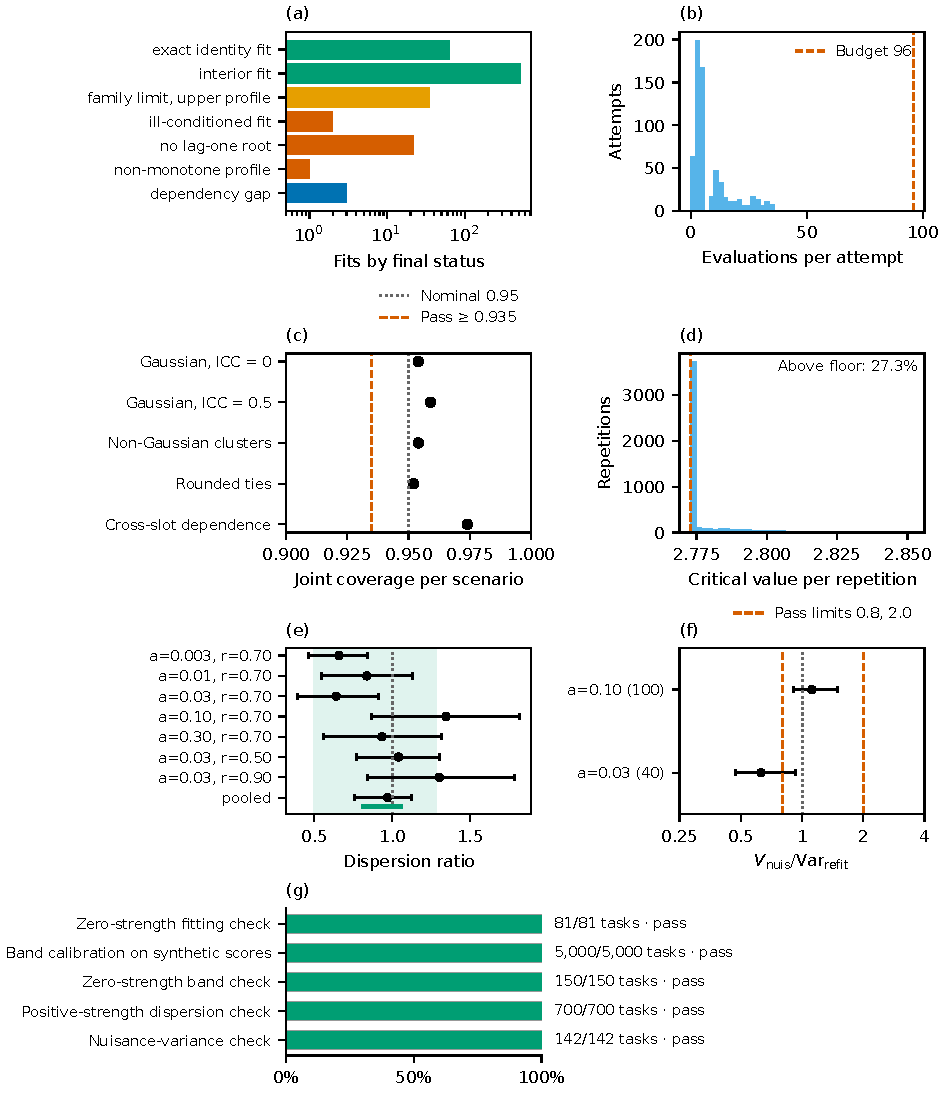
\includegraphics[width=\textwidth,height=150mm,keepaspectratio]{generated/J4_gate_diagnostics.pdf}
\caption{Validation-gate diagnostics from the public aggregates: (a) final fit statuses and (b) solver evaluations per attempt in the zero-strength fitting check (budget \resultnum{j.gate.solver_budget}{96}); (c) joint coverage per scenario and (d) critical values in the band calibration on synthetic scores, with the pass mark, nominal level and critical-value floor \resultnum{j.gate.critical_floor}{2.7729}; (e) dispersion ratios in the positive-strength dispersion check with bootstrap intervals and calibrated cell (shading) and pooled (green segment) thresholds; (f) local nuisance-variance estimates relative to full refits in the nuisance-variance check, with one-sided bounds; (g) completed tasks and verdict by stage. Family limits are gaps. The zero-strength band check uses its corrected aggregate record.}\label{fig:gate-diagnostics}
\end{figure}



\subsection{Execution, release and amendment v4.4}\label{sec:record-execution}\phantomsection\label{supp:execution-records}

\paragraph{Execution rules.}
The original operational deadline was 18 October 2026 at 23:59 America/Sao\_Paulo (19 October at 02:59 UTC). % M44 RC32
Eight shards executed the tiers in fixed order on a single host whose environment matched the one bound by the freeze record (see the article's Data and code availability statement; an operating-system update after the run changed that host's platform string, Section~\ref{sec:verification-limits}). AUC, band width or invalidity did not reorder them. % M44
The projected cost of the gate and all six tiers ranged from about 256 hours with measured costs to about 726 hours with 25\% retries. The latter exceeded the time between the freeze and the close, so tiers 3--6 could have been partial at the close, and their controls and sensitivities were not promised; in the event every tier finished (Section~\ref{sec:inventory}). % M80
At the close or release, each comparison/$r$ unit is recorded as not started, partial at the operational close, complete but invalid, or complete and valid, preserving attempts (Section~\ref{sec:inventory}). % M45
The main curve is valid only if all nine tier-1 units (B on the observed channel, one per $r$) are complete and valid in the released inventory. % M46
A tier-1 unit that is not started, partial or complete but invalid, for any reason, invalidates the main curve without deleting the boundaries of other units. Tier 1 therefore had to finish before the original deadline if early full-inventory release did not occur. % M46 RC33
The main curve could thus be invalidated by chance as well as by the clock. With a correct procedure and a critical value of at least 2.7729, the probability that one unit's $a=0$ band misses 0.5 is at most about 0.0056 under normal logit errors. If the nine B units are independent, the probability that at least one misses by chance alone is up to about 4.9\%. % M75

\paragraph{Release rule.}
A linked amendment registered on 28 September 2026, at the first author's instruction and before any tier started, permits release when all 414 units have final curve records and no curve worker is running, or at the original deadline; it permits no partial early release. Gate outcomes and curve estimates enter the results only through this release and its full inventory. % M85 RC34 M47
The frozen code remains revision \texttt{37513841}; the later release wrapper (Table~\ref{tab:record-identifiers}) implements this release rule without changing the grid, gates or inferential criteria. % M85 RC35 RC48
For an early release it passes the original deadline to the frozen release function, so the frozen record's close time keeps that conventional value. % M85 RC36 RC49
A separate release record supplies the actual release time, trigger, wrapper hash and released-output hash; the chronology needs both records. % M85 RC37

\paragraph{Shard incident and amendment v4.4.}
All five recorded gate stages passed, and the tiers started on 30 September 2026 (decision log item 114). On 1 October 2026 at 04:18 UTC, the worker of shard 5 ended during tier 2, and a relaunch with the frozen code failed in the same way. With the first author's authorization, the failure was reproduced on a copy of the unit outside the sealed store: in the cell at $a=0.003$ of the unit of D at $r=0.60$, the nuisance projection raised an ill-conditioned-local-profile error while propagating the nuisance, because the local profile Jacobian was degenerate, and the frozen runner does not handle that exception. Before this diagnosis, no tier-2 or later curve output had been read; only file counts, completion markers and modification times of that shard's units were inspected. % M89
Amendment v4.4, frozen in its own record, records a cell whose frozen execution ends with exactly that error, raised by the nuisance projection, as a sealed propagation gap with no attempt and with the hash of the successor runner that wrote it. Any other exception still ends the shard. The successor runner loads the frozen runner and runs its preflight and loop unchanged, replacing only the per-cell worker; it lives outside the frozen checkout, so the code hashes checked by the preflight and by shard resume are unchanged. A propagation gap follows the existing gap rules: at a positive strength it censors boundaries without invalidating the unit, and at $a=0$ it removes the zero-strength check. The inventory table reports it in its own column. % M89
The first author alone approved the amendment, the successor runner and the relaunch of the eight shards on 1 October at 14:33 UTC, during the second stage of the run: tier 1, the main curve against B, had finished and stayed sealed and unread, and no tier-2 or later curve output had been read. The amendment recorded that scientific ratification, with the supervisor's review, was still pending; it was covered by the ratification recorded later that day (decision log item 161), before the results became available. The shard resumed past its completed cells and recorded the gap at 14:35 UTC. Completed cells were not rerun. % M89
The rule applied to two cells, both at $a=0.003$ and $r=0.60$: the unit of D on the observed channel (\resultnum{v4.tab.T4.2-D-observed-main.gaps_propagation}{1} propagation gap) and the matching mobility unit of D (\resultnum{v4.tab.T4.3-D-observed-mobility.gaps_propagation}{1}). Its consequence for the reported results is confined to D at $r=0.60$: the first boundary against D there is censored at the propagation gap, $a=\resultnum{v4.tab.T1.D.r060.a_star.1}{0.003}$, while the next gap of that unit is a family limit at $a=\resultnum{j.models.D.r060.first.gap.1.a}{0.10}$, the first gap of D at seven of the other eight shares. Read after the results became available: below that family limit the point AUC against D stayed near 0.5 at $r=0.60$ (\resultnum{j.models.D.r060.a0100.auc}{0.506} at $a=0.01$ and \resultnum{j.models.D.r060.a0300.auc}{0.519} at 0.03), and every first and sustained boundary against D is censored at all nine shares (Section~\ref{sec:additional-models}), so the amendment moved the censoring point at that share without changing whether any comparison with D could be read. The sentence of the rule-assembled introduction that ``every reporting rule was fixed before any confirmatory result was released'' therefore holds only in this qualified sense: v4.4, an operational rule that decides how one kind of failure is recorded, was approved during the run, after the main curve had been computed and before any result was read or released.

\paragraph{Release chronology.}
% Moved from sections/results.tex (Release and unit inventory) of the rule-assembled attempt.
The results became available on \resultnum{v4.release.effective_local}{8 October 2026 at 11:26:02} America/Sao\_Paulo, triggered by \resultnum{v4.release.condition}{completion of the full inventory}; the nominal close was \resultnum{v4.protocol.close_local}{18 October 2026 at 23:59} America/Sao\_Paulo. The tiers ran in the fixed order, without changes based on AUC, band width or invalidity. No work was unfinished at release, so the declared-close rule did not have to stop any; only complete units contribute boundaries and AUC profiles (Section~\ref{sec:inventory}).

\subsection{Governance and ratification}\label{sec:record-governance}

The v1 protocol was frozen by the coordinating agent under the first author's delegation (decision log item 18), and the v4 decision specification records a delegated agent decision (decision log item 19); both records mark these decisions as pending ratification, and both took effect before that ratification. The authors ratified both, together with the later amendments and delegated decisions, on 1 October 2026, before the results became available (decision log item 161). % M83
The ratification record states the scope: v1 as history, v4 amended after partial exposure, amendment v4.4, the delegated decisions, the exploratory declarations and the interpretation rules; it records that acceptance of the released results could not be anticipated and is left to both authors' reading of the final manuscript. The release amendment of 28 September 2026 followed an explicit instruction of the first author; Section~\ref{sec:ai} describes the use of AI agents in these steps.

\clearpage


\section{Unit inventory}\label{sec:inventory}
% Unit inventory (Section S5). Written during the journal revision (agent S,
% 2026-10-13) from the inventory paragraphs of sections/results.tex and the
% status rules of the rule-assembled attempt; the split of the invalid units
% by cause tabulates the released curves (public aggregates, cell at a = 0).
% Round 6: cites the plain-text README uploaded with Online Resource 2.

The prespecified inventory has 46 comparison grids, each crossed with the nine signal shares and the nine strengths of influence: \resultnum{v4.protocol.units.all}{414} units of nine cells each. A unit is one comparison (persistence model, channel and configuration) at one $r$. Its status at the close or release is one of four:
\begin{description}
\item[Complete and valid.] All nine strengths were executed, and the zero-strength cell is available with a band containing 0.5. Gaps at positive strengths censor boundaries but do not invalidate the unit.
\item[Complete but invalid.] All nine strengths were executed, but the zero-strength check failed: the band at $a=0$ excluded 0.5, or the zero-strength cell was a gap. The unit's boundaries are suppressed; its cells stay in the records.
\item[Partial at the operational close.] Some strengths were not executed when the compute window closed.
\item[Not started.] No strength was executed at the close.
\end{description}
These statuses are operational categories of the protocol: ``valid'' records that the zero-strength check passed, not that the unit's intervals have been shown to cover. The main curve is valid only if all nine units of B on the observed channel are complete and valid. The archived machine-readable inventory stores these statuses as Portuguese strings; Table~\ref{tab:glossary-states} maps them to the names used here.

When the results became available, \resultnum{v4.inv.n_valid}{342} of the \resultnum{v4.protocol.units.all}{414} units were complete and valid, \resultnum{v4.inv.n_invalid}{72} were complete but invalid, \resultnum{v4.inv.n_partial}{0} were partial at the operational close and \resultnum{v4.inv.n_not_started}{0} had not started (Table~\ref{tab:v4-T4}, Fig.~\ref{fig:inventory-status}). Every tier therefore finished. By tier: all \resultnum{v4.tab.T4.1-all-all-all.valid}{9} units of the main curve against B were complete and valid, so the main curve is valid under the frozen rule; of the \resultnum{v4.tab.T4.2-all-all-all.units}{36} units of the secondary persistence models, \resultnum{v4.tab.T4.2-all-all-all.valid}{27} were complete and valid and \resultnum{v4.inv.t2.n_invalid}{9} complete but invalid; the measurement-control tier ended with \resultnum{v4.inv.t3.n_valid}{243} of its \resultnum{v4.protocol.units.t3}{270} units complete and valid and \resultnum{v4.inv.t3.n_incomplete}{0} not started or partial; \resultnum{v4.inv.t4.n_valid}{45} of \resultnum{v4.protocol.units.t4}{45} response-channel units and \resultnum{v4.inv.t5.n_valid}{9} of \resultnum{v4.protocol.units.t5}{45} mechanism units were complete and valid; and of the \resultnum{v4.protocol.units.t6}{9} units with \resultnum{v4.protocol.steps}{24} update steps per wave, \resultnum{v4.inv.t6.n_valid}{9} were complete and valid. Only complete units contribute boundaries and AUC profiles.

\paragraph{The 72 invalid units, by cause.}
All \resultnum{j.inventory.invalid.total}{72} complete-but-invalid units fall into two groups, with \resultnum{j.inventory.invalid.other}{0} units outside them.
\begin{itemize}
\item \resultnum{j.inventory.invalid.c_related}{36} units involve persistence model C, whose persistence arm alone receives heteroscedastic error and heaping, so that the two arms differ at zero strength by construction. In the \resultnum{v4.tab.T4.2-C-observed-main.invalid}{9} units of the other-models comparison and the \resultnum{v4.tab.T4.3-C-observed-mobility.invalid}{9} mobility units on the observed channel, the band at $a=0$ excluded 0.5: the zero-strength point AUC against C was \resultnum{j.models.C.zero_auc.min}{1.000} at every share. In \resultnum{v4.tab.T4.3-C-latent-main.invalid}{7} latent-control units, \resultnum{v4.tab.T4.3-C-latent-rank-main.invalid}{4} latent-rank-control units and \resultnum{v4.tab.T4.3-C-latent-mobility.invalid}{7} latent mobility units of C, the zero-strength cell was a gap because the accepted fit failed independent validation in both attempts.
\item \resultnum{j.inventory.invalid.anchoring_sensitivities}{36} units are the anchoring sensitivities, nine for each $\omega\in\{0.25,0.50,0.75,1\}$. With $\omega>0$ the influence arm is pulled toward its initial states at every step, while B has no anchoring, so no identity of the arms at zero strength is claimed; with $\omega=1$ the latent states never change, whatever $a$ is. At $\omega=0.25$ the band at $a=0$ excluded 0.5 in all \resultnum{v4.tab.T4.5-B-observed-omega025.invalid}{9} units. At $\omega=0.50$ the zero-strength cell was a family-limit gap in all \resultnum{v4.tab.T4.5-B-observed-omega050.invalid}{9} units; at $\omega=0.75$ it was a family-limit gap in \resultnum{j.inventory.invalid.omega075.zero_gap.family_limit}{5} units and another solver gap in \resultnum{j.inventory.invalid.omega075.zero_gap.solver}{4}; at $\omega=1$, a family-limit gap in \resultnum{j.inventory.invalid.omega100.zero_gap.family_limit}{2} and another solver gap in \resultnum{j.inventory.invalid.omega100.zero_gap.solver}{7}. These units carry no information about $a$: they check that the anchored arm and B differ at zero strength, which they do by construction.
\end{itemize}

\paragraph{Gap cells.}
The inventory also counts the gap cells of the released curves by kind. In the control units, \resultnum{v4.t3.gap.dependency}{330} cells are dependency gaps because the observed fit they reuse failed or is missing. The two propagation gaps recorded under amendment v4.4 are both in units of D at $r=0.60$ (Section~\ref{sec:record-execution}). Gaps are never counted as AUCs below the target or as evidence that separation is impossible; family limits are gaps, not failures.

\paragraph{Online Resource 2.}
Online Resource~2 (\code{online-resource-2-units.csv}) is the table of all units in English, uploaded with a plain-text README that lists its columns, the scenario legend and the translation of the status labels. It is derived from the released all-units table: it keeps the same rows and columns and translates the Portuguese labels into the names used here, with no other change. The released original, with its Portuguese status labels, stays in the archive. The table gives, for every unit, its tier, persistence model, channel, configuration, $r$, the mark of the share examined during calibration (column \code{exposure}, which keeps the record term calibration-exposed), the main-curve flag (empty in every row, because the main curve is valid), status, zero-strength check (column \code{null_gate}), gap counts by kind, first and sustained boundaries with their intervals, region (with the labels of Table~\ref{tab:glossary-terms}; ``censored (gap)'' is the censored label), the boundaries at the secondary targets 0.60 and 0.80, the band-monotonicity flag, the critical value and whether it exceeded the 2.7729 floor.

% Generated by ic_study.analysis.v4_report_export from the v4 report with
% manifest SHA-256 6608b3960eb73011caca97870a4ffd3dbfbcd4c2df09bbbcb576c1c9452cf981.
% Edited during the journal revision (agent S, 2026-10-13): captions, headers and
% categorical cells in plain English; every number keeps its \resultnum binding.
\begin{table*}[tp]
\caption{Inventory at the close: units by status for each prespecified configuration, for each tier and in total, and the gap cells of the released curves by kind. Tiers: 1 main curve against B; 2 secondary persistence models; 3 measurement controls (latent, ordinal with $r=1$, latent rank) and mobility summaries; 4 response-channel sensitivities (persistent response style, $c=0.25$ or 0.50; panel conditioning, $\delta=0.10$ or 0.20; response style and conditioning, $c=0.50$, $\delta=0.20$, exploratory); 5 mechanism sensitivities (attraction only, $b=0$; anchoring; complete anchoring, $\omega=1$); 6 24 update steps per wave (Table~\ref{tab:glossary-gate}). Status: NS not started, P partial at the operational close, CI complete but invalid, CV complete and valid (Section~\ref{sec:inventory}; the archive's machine-readable records store these four statuses in Portuguese). Gap cells: scr.\ family limit at the feasibility screen, with no solver evaluation; fam.\ family limit on the profile; sol.\ other solver status; val.\ accepted fit that failed validation in both attempts; dep.\ control whose observed fit failed or is missing; prop.\ ill-conditioned nuisance propagation recorded as a gap under amendment v4.4 (Section~\ref{sec:record-execution}). Family limits are gaps, not failures.}\label{tab:v4-T4}
\centering\scriptsize
\setlength{\tabcolsep}{1.5pt}
\begin{tabular}{lllp{2.3cm}rrrrrrrrrrr}
\toprule
Tier & Model & Channel & Configuration & Units & NS & P & CI & CV & scr. & fam. & sol. & val. & dep. & prop. \\
\midrule
\resultnum{v4.tab.T4.1-B-observed-main.tier}{1} & B & observed & main & \resultnum{v4.tab.T4.1-B-observed-main.units}{9} & \resultnum{v4.tab.T4.1-B-observed-main.not_started}{0} & \resultnum{v4.tab.T4.1-B-observed-main.partial}{0} & \resultnum{v4.tab.T4.1-B-observed-main.invalid}{0} & \resultnum{v4.tab.T4.1-B-observed-main.valid}{9} & \resultnum{v4.tab.T4.1-B-observed-main.gaps_screened}{0} & \resultnum{v4.tab.T4.1-B-observed-main.gaps_family_limit}{0} & \resultnum{v4.tab.T4.1-B-observed-main.gaps_solver}{3} & \resultnum{v4.tab.T4.1-B-observed-main.gaps_validation}{0} & \resultnum{v4.tab.T4.1-B-observed-main.gaps_dependency}{0} & \resultnum{v4.tab.T4.1-B-observed-main.gaps_propagation}{0} \\
\resultnum{v4.tab.T4.2-A-observed-main.tier}{2} & A & observed & main & \resultnum{v4.tab.T4.2-A-observed-main.units}{9} & \resultnum{v4.tab.T4.2-A-observed-main.not_started}{0} & \resultnum{v4.tab.T4.2-A-observed-main.partial}{0} & \resultnum{v4.tab.T4.2-A-observed-main.invalid}{0} & \resultnum{v4.tab.T4.2-A-observed-main.valid}{9} & \resultnum{v4.tab.T4.2-A-observed-main.gaps_screened}{0} & \resultnum{v4.tab.T4.2-A-observed-main.gaps_family_limit}{0} & \resultnum{v4.tab.T4.2-A-observed-main.gaps_solver}{0} & \resultnum{v4.tab.T4.2-A-observed-main.gaps_validation}{0} & \resultnum{v4.tab.T4.2-A-observed-main.gaps_dependency}{0} & \resultnum{v4.tab.T4.2-A-observed-main.gaps_propagation}{0} \\
\resultnum{v4.tab.T4.2-C-observed-main.tier}{2} & C & observed & main & \resultnum{v4.tab.T4.2-C-observed-main.units}{9} & \resultnum{v4.tab.T4.2-C-observed-main.not_started}{0} & \resultnum{v4.tab.T4.2-C-observed-main.partial}{0} & \resultnum{v4.tab.T4.2-C-observed-main.invalid}{9} & \resultnum{v4.tab.T4.2-C-observed-main.valid}{0} & \resultnum{v4.tab.T4.2-C-observed-main.gaps_screened}{0} & \resultnum{v4.tab.T4.2-C-observed-main.gaps_family_limit}{0} & \resultnum{v4.tab.T4.2-C-observed-main.gaps_solver}{22} & \resultnum{v4.tab.T4.2-C-observed-main.gaps_validation}{0} & \resultnum{v4.tab.T4.2-C-observed-main.gaps_dependency}{0} & \resultnum{v4.tab.T4.2-C-observed-main.gaps_propagation}{0} \\
\resultnum{v4.tab.T4.2-D-observed-main.tier}{2} & D & observed & main & \resultnum{v4.tab.T4.2-D-observed-main.units}{9} & \resultnum{v4.tab.T4.2-D-observed-main.not_started}{0} & \resultnum{v4.tab.T4.2-D-observed-main.partial}{0} & \resultnum{v4.tab.T4.2-D-observed-main.invalid}{0} & \resultnum{v4.tab.T4.2-D-observed-main.valid}{9} & \resultnum{v4.tab.T4.2-D-observed-main.gaps_screened}{0} & \resultnum{v4.tab.T4.2-D-observed-main.gaps_family_limit}{33} & \resultnum{v4.tab.T4.2-D-observed-main.gaps_solver}{4} & \resultnum{v4.tab.T4.2-D-observed-main.gaps_validation}{0} & \resultnum{v4.tab.T4.2-D-observed-main.gaps_dependency}{0} & \resultnum{v4.tab.T4.2-D-observed-main.gaps_propagation}{1} \\
\resultnum{v4.tab.T4.2-E-observed-main.tier}{2} & E & observed & main & \resultnum{v4.tab.T4.2-E-observed-main.units}{9} & \resultnum{v4.tab.T4.2-E-observed-main.not_started}{0} & \resultnum{v4.tab.T4.2-E-observed-main.partial}{0} & \resultnum{v4.tab.T4.2-E-observed-main.invalid}{0} & \resultnum{v4.tab.T4.2-E-observed-main.valid}{9} & \resultnum{v4.tab.T4.2-E-observed-main.gaps_screened}{0} & \resultnum{v4.tab.T4.2-E-observed-main.gaps_family_limit}{0} & \resultnum{v4.tab.T4.2-E-observed-main.gaps_solver}{3} & \resultnum{v4.tab.T4.2-E-observed-main.gaps_validation}{0} & \resultnum{v4.tab.T4.2-E-observed-main.gaps_dependency}{0} & \resultnum{v4.tab.T4.2-E-observed-main.gaps_propagation}{0} \\
\resultnum{v4.tab.T4.3-A-latent-main.tier}{3} & A & latent & main & \resultnum{v4.tab.T4.3-A-latent-main.units}{9} & \resultnum{v4.tab.T4.3-A-latent-main.not_started}{0} & \resultnum{v4.tab.T4.3-A-latent-main.partial}{0} & \resultnum{v4.tab.T4.3-A-latent-main.invalid}{0} & \resultnum{v4.tab.T4.3-A-latent-main.valid}{9} & \resultnum{v4.tab.T4.3-A-latent-main.gaps_screened}{0} & \resultnum{v4.tab.T4.3-A-latent-main.gaps_family_limit}{0} & \resultnum{v4.tab.T4.3-A-latent-main.gaps_solver}{0} & \resultnum{v4.tab.T4.3-A-latent-main.gaps_validation}{0} & \resultnum{v4.tab.T4.3-A-latent-main.gaps_dependency}{0} & \resultnum{v4.tab.T4.3-A-latent-main.gaps_propagation}{0} \\
\resultnum{v4.tab.T4.3-A-ordinal-one-main.tier}{3} & A & ordinal, $r=1$ & main & \resultnum{v4.tab.T4.3-A-ordinal-one-main.units}{9} & \resultnum{v4.tab.T4.3-A-ordinal-one-main.not_started}{0} & \resultnum{v4.tab.T4.3-A-ordinal-one-main.partial}{0} & \resultnum{v4.tab.T4.3-A-ordinal-one-main.invalid}{0} & \resultnum{v4.tab.T4.3-A-ordinal-one-main.valid}{9} & \resultnum{v4.tab.T4.3-A-ordinal-one-main.gaps_screened}{0} & \resultnum{v4.tab.T4.3-A-ordinal-one-main.gaps_family_limit}{0} & \resultnum{v4.tab.T4.3-A-ordinal-one-main.gaps_solver}{0} & \resultnum{v4.tab.T4.3-A-ordinal-one-main.gaps_validation}{0} & \resultnum{v4.tab.T4.3-A-ordinal-one-main.gaps_dependency}{0} & \resultnum{v4.tab.T4.3-A-ordinal-one-main.gaps_propagation}{0} \\
\resultnum{v4.tab.T4.3-A-latent-rank-main.tier}{3} & A & latent rank & main & \resultnum{v4.tab.T4.3-A-latent-rank-main.units}{9} & \resultnum{v4.tab.T4.3-A-latent-rank-main.not_started}{0} & \resultnum{v4.tab.T4.3-A-latent-rank-main.partial}{0} & \resultnum{v4.tab.T4.3-A-latent-rank-main.invalid}{0} & \resultnum{v4.tab.T4.3-A-latent-rank-main.valid}{9} & \resultnum{v4.tab.T4.3-A-latent-rank-main.gaps_screened}{0} & \resultnum{v4.tab.T4.3-A-latent-rank-main.gaps_family_limit}{0} & \resultnum{v4.tab.T4.3-A-latent-rank-main.gaps_solver}{0} & \resultnum{v4.tab.T4.3-A-latent-rank-main.gaps_validation}{0} & \resultnum{v4.tab.T4.3-A-latent-rank-main.gaps_dependency}{0} & \resultnum{v4.tab.T4.3-A-latent-rank-main.gaps_propagation}{0} \\
\resultnum{v4.tab.T4.3-B-latent-main.tier}{3} & B & latent & main & \resultnum{v4.tab.T4.3-B-latent-main.units}{9} & \resultnum{v4.tab.T4.3-B-latent-main.not_started}{0} & \resultnum{v4.tab.T4.3-B-latent-main.partial}{0} & \resultnum{v4.tab.T4.3-B-latent-main.invalid}{0} & \resultnum{v4.tab.T4.3-B-latent-main.valid}{9} & \resultnum{v4.tab.T4.3-B-latent-main.gaps_screened}{0} & \resultnum{v4.tab.T4.3-B-latent-main.gaps_family_limit}{0} & \resultnum{v4.tab.T4.3-B-latent-main.gaps_solver}{0} & \resultnum{v4.tab.T4.3-B-latent-main.gaps_validation}{0} & \resultnum{v4.tab.T4.3-B-latent-main.gaps_dependency}{3} & \resultnum{v4.tab.T4.3-B-latent-main.gaps_propagation}{0} \\
\resultnum{v4.tab.T4.3-B-ordinal-one-main.tier}{3} & B & ordinal, $r=1$ & main & \resultnum{v4.tab.T4.3-B-ordinal-one-main.units}{9} & \resultnum{v4.tab.T4.3-B-ordinal-one-main.not_started}{0} & \resultnum{v4.tab.T4.3-B-ordinal-one-main.partial}{0} & \resultnum{v4.tab.T4.3-B-ordinal-one-main.invalid}{0} & \resultnum{v4.tab.T4.3-B-ordinal-one-main.valid}{9} & \resultnum{v4.tab.T4.3-B-ordinal-one-main.gaps_screened}{0} & \resultnum{v4.tab.T4.3-B-ordinal-one-main.gaps_family_limit}{0} & \resultnum{v4.tab.T4.3-B-ordinal-one-main.gaps_solver}{0} & \resultnum{v4.tab.T4.3-B-ordinal-one-main.gaps_validation}{0} & \resultnum{v4.tab.T4.3-B-ordinal-one-main.gaps_dependency}{3} & \resultnum{v4.tab.T4.3-B-ordinal-one-main.gaps_propagation}{0} \\
\resultnum{v4.tab.T4.3-B-latent-rank-main.tier}{3} & B & latent rank & main & \resultnum{v4.tab.T4.3-B-latent-rank-main.units}{9} & \resultnum{v4.tab.T4.3-B-latent-rank-main.not_started}{0} & \resultnum{v4.tab.T4.3-B-latent-rank-main.partial}{0} & \resultnum{v4.tab.T4.3-B-latent-rank-main.invalid}{0} & \resultnum{v4.tab.T4.3-B-latent-rank-main.valid}{9} & \resultnum{v4.tab.T4.3-B-latent-rank-main.gaps_screened}{0} & \resultnum{v4.tab.T4.3-B-latent-rank-main.gaps_family_limit}{0} & \resultnum{v4.tab.T4.3-B-latent-rank-main.gaps_solver}{0} & \resultnum{v4.tab.T4.3-B-latent-rank-main.gaps_validation}{0} & \resultnum{v4.tab.T4.3-B-latent-rank-main.gaps_dependency}{3} & \resultnum{v4.tab.T4.3-B-latent-rank-main.gaps_propagation}{0} \\
\resultnum{v4.tab.T4.3-C-latent-main.tier}{3} & C & latent & main & \resultnum{v4.tab.T4.3-C-latent-main.units}{9} & \resultnum{v4.tab.T4.3-C-latent-main.not_started}{0} & \resultnum{v4.tab.T4.3-C-latent-main.partial}{0} & \resultnum{v4.tab.T4.3-C-latent-main.invalid}{7} & \resultnum{v4.tab.T4.3-C-latent-main.valid}{2} & \resultnum{v4.tab.T4.3-C-latent-main.gaps_screened}{0} & \resultnum{v4.tab.T4.3-C-latent-main.gaps_family_limit}{0} & \resultnum{v4.tab.T4.3-C-latent-main.gaps_solver}{0} & \resultnum{v4.tab.T4.3-C-latent-main.gaps_validation}{7} & \resultnum{v4.tab.T4.3-C-latent-main.gaps_dependency}{22} & \resultnum{v4.tab.T4.3-C-latent-main.gaps_propagation}{0} \\
\resultnum{v4.tab.T4.3-C-ordinal-one-main.tier}{3} & C & ordinal, $r=1$ & main & \resultnum{v4.tab.T4.3-C-ordinal-one-main.units}{9} & \resultnum{v4.tab.T4.3-C-ordinal-one-main.not_started}{0} & \resultnum{v4.tab.T4.3-C-ordinal-one-main.partial}{0} & \resultnum{v4.tab.T4.3-C-ordinal-one-main.invalid}{0} & \resultnum{v4.tab.T4.3-C-ordinal-one-main.valid}{9} & \resultnum{v4.tab.T4.3-C-ordinal-one-main.gaps_screened}{0} & \resultnum{v4.tab.T4.3-C-ordinal-one-main.gaps_family_limit}{0} & \resultnum{v4.tab.T4.3-C-ordinal-one-main.gaps_solver}{0} & \resultnum{v4.tab.T4.3-C-ordinal-one-main.gaps_validation}{0} & \resultnum{v4.tab.T4.3-C-ordinal-one-main.gaps_dependency}{22} & \resultnum{v4.tab.T4.3-C-ordinal-one-main.gaps_propagation}{0} \\
\resultnum{v4.tab.T4.3-C-latent-rank-main.tier}{3} & C & latent rank & main & \resultnum{v4.tab.T4.3-C-latent-rank-main.units}{9} & \resultnum{v4.tab.T4.3-C-latent-rank-main.not_started}{0} & \resultnum{v4.tab.T4.3-C-latent-rank-main.partial}{0} & \resultnum{v4.tab.T4.3-C-latent-rank-main.invalid}{4} & \resultnum{v4.tab.T4.3-C-latent-rank-main.valid}{5} & \resultnum{v4.tab.T4.3-C-latent-rank-main.gaps_screened}{0} & \resultnum{v4.tab.T4.3-C-latent-rank-main.gaps_family_limit}{0} & \resultnum{v4.tab.T4.3-C-latent-rank-main.gaps_solver}{0} & \resultnum{v4.tab.T4.3-C-latent-rank-main.gaps_validation}{4} & \resultnum{v4.tab.T4.3-C-latent-rank-main.gaps_dependency}{22} & \resultnum{v4.tab.T4.3-C-latent-rank-main.gaps_propagation}{0} \\
\resultnum{v4.tab.T4.3-D-latent-main.tier}{3} & D & latent & main & \resultnum{v4.tab.T4.3-D-latent-main.units}{9} & \resultnum{v4.tab.T4.3-D-latent-main.not_started}{0} & \resultnum{v4.tab.T4.3-D-latent-main.partial}{0} & \resultnum{v4.tab.T4.3-D-latent-main.invalid}{0} & \resultnum{v4.tab.T4.3-D-latent-main.valid}{9} & \resultnum{v4.tab.T4.3-D-latent-main.gaps_screened}{0} & \resultnum{v4.tab.T4.3-D-latent-main.gaps_family_limit}{0} & \resultnum{v4.tab.T4.3-D-latent-main.gaps_solver}{0} & \resultnum{v4.tab.T4.3-D-latent-main.gaps_validation}{0} & \resultnum{v4.tab.T4.3-D-latent-main.gaps_dependency}{38} & \resultnum{v4.tab.T4.3-D-latent-main.gaps_propagation}{0} \\
\resultnum{v4.tab.T4.3-D-ordinal-one-main.tier}{3} & D & ordinal, $r=1$ & main & \resultnum{v4.tab.T4.3-D-ordinal-one-main.units}{9} & \resultnum{v4.tab.T4.3-D-ordinal-one-main.not_started}{0} & \resultnum{v4.tab.T4.3-D-ordinal-one-main.partial}{0} & \resultnum{v4.tab.T4.3-D-ordinal-one-main.invalid}{0} & \resultnum{v4.tab.T4.3-D-ordinal-one-main.valid}{9} & \resultnum{v4.tab.T4.3-D-ordinal-one-main.gaps_screened}{0} & \resultnum{v4.tab.T4.3-D-ordinal-one-main.gaps_family_limit}{0} & \resultnum{v4.tab.T4.3-D-ordinal-one-main.gaps_solver}{0} & \resultnum{v4.tab.T4.3-D-ordinal-one-main.gaps_validation}{0} & \resultnum{v4.tab.T4.3-D-ordinal-one-main.gaps_dependency}{38} & \resultnum{v4.tab.T4.3-D-ordinal-one-main.gaps_propagation}{0} \\
\resultnum{v4.tab.T4.3-D-latent-rank-main.tier}{3} & D & latent rank & main & \resultnum{v4.tab.T4.3-D-latent-rank-main.units}{9} & \resultnum{v4.tab.T4.3-D-latent-rank-main.not_started}{0} & \resultnum{v4.tab.T4.3-D-latent-rank-main.partial}{0} & \resultnum{v4.tab.T4.3-D-latent-rank-main.invalid}{0} & \resultnum{v4.tab.T4.3-D-latent-rank-main.valid}{9} & \resultnum{v4.tab.T4.3-D-latent-rank-main.gaps_screened}{0} & \resultnum{v4.tab.T4.3-D-latent-rank-main.gaps_family_limit}{0} & \resultnum{v4.tab.T4.3-D-latent-rank-main.gaps_solver}{0} & \resultnum{v4.tab.T4.3-D-latent-rank-main.gaps_validation}{0} & \resultnum{v4.tab.T4.3-D-latent-rank-main.gaps_dependency}{38} & \resultnum{v4.tab.T4.3-D-latent-rank-main.gaps_propagation}{0} \\
\resultnum{v4.tab.T4.3-E-latent-main.tier}{3} & E & latent & main & \resultnum{v4.tab.T4.3-E-latent-main.units}{9} & \resultnum{v4.tab.T4.3-E-latent-main.not_started}{0} & \resultnum{v4.tab.T4.3-E-latent-main.partial}{0} & \resultnum{v4.tab.T4.3-E-latent-main.invalid}{0} & \resultnum{v4.tab.T4.3-E-latent-main.valid}{9} & \resultnum{v4.tab.T4.3-E-latent-main.gaps_screened}{0} & \resultnum{v4.tab.T4.3-E-latent-main.gaps_family_limit}{0} & \resultnum{v4.tab.T4.3-E-latent-main.gaps_solver}{0} & \resultnum{v4.tab.T4.3-E-latent-main.gaps_validation}{0} & \resultnum{v4.tab.T4.3-E-latent-main.gaps_dependency}{3} & \resultnum{v4.tab.T4.3-E-latent-main.gaps_propagation}{0} \\
\resultnum{v4.tab.T4.3-E-ordinal-one-main.tier}{3} & E & ordinal, $r=1$ & main & \resultnum{v4.tab.T4.3-E-ordinal-one-main.units}{9} & \resultnum{v4.tab.T4.3-E-ordinal-one-main.not_started}{0} & \resultnum{v4.tab.T4.3-E-ordinal-one-main.partial}{0} & \resultnum{v4.tab.T4.3-E-ordinal-one-main.invalid}{0} & \resultnum{v4.tab.T4.3-E-ordinal-one-main.valid}{9} & \resultnum{v4.tab.T4.3-E-ordinal-one-main.gaps_screened}{0} & \resultnum{v4.tab.T4.3-E-ordinal-one-main.gaps_family_limit}{0} & \resultnum{v4.tab.T4.3-E-ordinal-one-main.gaps_solver}{0} & \resultnum{v4.tab.T4.3-E-ordinal-one-main.gaps_validation}{0} & \resultnum{v4.tab.T4.3-E-ordinal-one-main.gaps_dependency}{3} & \resultnum{v4.tab.T4.3-E-ordinal-one-main.gaps_propagation}{0} \\
\resultnum{v4.tab.T4.3-E-latent-rank-main.tier}{3} & E & latent rank & main & \resultnum{v4.tab.T4.3-E-latent-rank-main.units}{9} & \resultnum{v4.tab.T4.3-E-latent-rank-main.not_started}{0} & \resultnum{v4.tab.T4.3-E-latent-rank-main.partial}{0} & \resultnum{v4.tab.T4.3-E-latent-rank-main.invalid}{0} & \resultnum{v4.tab.T4.3-E-latent-rank-main.valid}{9} & \resultnum{v4.tab.T4.3-E-latent-rank-main.gaps_screened}{0} & \resultnum{v4.tab.T4.3-E-latent-rank-main.gaps_family_limit}{0} & \resultnum{v4.tab.T4.3-E-latent-rank-main.gaps_solver}{0} & \resultnum{v4.tab.T4.3-E-latent-rank-main.gaps_validation}{0} & \resultnum{v4.tab.T4.3-E-latent-rank-main.gaps_dependency}{3} & \resultnum{v4.tab.T4.3-E-latent-rank-main.gaps_propagation}{0} \\
\resultnum{v4.tab.T4.3-A-observed-mobility.tier}{3} & A & observed & mobility & \resultnum{v4.tab.T4.3-A-observed-mobility.units}{9} & \resultnum{v4.tab.T4.3-A-observed-mobility.not_started}{0} & \resultnum{v4.tab.T4.3-A-observed-mobility.partial}{0} & \resultnum{v4.tab.T4.3-A-observed-mobility.invalid}{0} & \resultnum{v4.tab.T4.3-A-observed-mobility.valid}{9} & \resultnum{v4.tab.T4.3-A-observed-mobility.gaps_screened}{0} & \resultnum{v4.tab.T4.3-A-observed-mobility.gaps_family_limit}{0} & \resultnum{v4.tab.T4.3-A-observed-mobility.gaps_solver}{0} & \resultnum{v4.tab.T4.3-A-observed-mobility.gaps_validation}{0} & \resultnum{v4.tab.T4.3-A-observed-mobility.gaps_dependency}{0} & \resultnum{v4.tab.T4.3-A-observed-mobility.gaps_propagation}{0} \\
\resultnum{v4.tab.T4.3-A-latent-mobility.tier}{3} & A & latent & mobility & \resultnum{v4.tab.T4.3-A-latent-mobility.units}{9} & \resultnum{v4.tab.T4.3-A-latent-mobility.not_started}{0} & \resultnum{v4.tab.T4.3-A-latent-mobility.partial}{0} & \resultnum{v4.tab.T4.3-A-latent-mobility.invalid}{0} & \resultnum{v4.tab.T4.3-A-latent-mobility.valid}{9} & \resultnum{v4.tab.T4.3-A-latent-mobility.gaps_screened}{0} & \resultnum{v4.tab.T4.3-A-latent-mobility.gaps_family_limit}{0} & \resultnum{v4.tab.T4.3-A-latent-mobility.gaps_solver}{0} & \resultnum{v4.tab.T4.3-A-latent-mobility.gaps_validation}{0} & \resultnum{v4.tab.T4.3-A-latent-mobility.gaps_dependency}{0} & \resultnum{v4.tab.T4.3-A-latent-mobility.gaps_propagation}{0} \\
\resultnum{v4.tab.T4.3-A-ordinal-one-mobility.tier}{3} & A & ordinal, $r=1$ & mobility & \resultnum{v4.tab.T4.3-A-ordinal-one-mobility.units}{9} & \resultnum{v4.tab.T4.3-A-ordinal-one-mobility.not_started}{0} & \resultnum{v4.tab.T4.3-A-ordinal-one-mobility.partial}{0} & \resultnum{v4.tab.T4.3-A-ordinal-one-mobility.invalid}{0} & \resultnum{v4.tab.T4.3-A-ordinal-one-mobility.valid}{9} & \resultnum{v4.tab.T4.3-A-ordinal-one-mobility.gaps_screened}{0} & \resultnum{v4.tab.T4.3-A-ordinal-one-mobility.gaps_family_limit}{0} & \resultnum{v4.tab.T4.3-A-ordinal-one-mobility.gaps_solver}{0} & \resultnum{v4.tab.T4.3-A-ordinal-one-mobility.gaps_validation}{0} & \resultnum{v4.tab.T4.3-A-ordinal-one-mobility.gaps_dependency}{0} & \resultnum{v4.tab.T4.3-A-ordinal-one-mobility.gaps_propagation}{0} \\
\resultnum{v4.tab.T4.3-B-observed-mobility.tier}{3} & B & observed & mobility & \resultnum{v4.tab.T4.3-B-observed-mobility.units}{9} & \resultnum{v4.tab.T4.3-B-observed-mobility.not_started}{0} & \resultnum{v4.tab.T4.3-B-observed-mobility.partial}{0} & \resultnum{v4.tab.T4.3-B-observed-mobility.invalid}{0} & \resultnum{v4.tab.T4.3-B-observed-mobility.valid}{9} & \resultnum{v4.tab.T4.3-B-observed-mobility.gaps_screened}{0} & \resultnum{v4.tab.T4.3-B-observed-mobility.gaps_family_limit}{0} & \resultnum{v4.tab.T4.3-B-observed-mobility.gaps_solver}{3} & \resultnum{v4.tab.T4.3-B-observed-mobility.gaps_validation}{0} & \resultnum{v4.tab.T4.3-B-observed-mobility.gaps_dependency}{0} & \resultnum{v4.tab.T4.3-B-observed-mobility.gaps_propagation}{0} \\
\resultnum{v4.tab.T4.3-B-latent-mobility.tier}{3} & B & latent & mobility & \resultnum{v4.tab.T4.3-B-latent-mobility.units}{9} & \resultnum{v4.tab.T4.3-B-latent-mobility.not_started}{0} & \resultnum{v4.tab.T4.3-B-latent-mobility.partial}{0} & \resultnum{v4.tab.T4.3-B-latent-mobility.invalid}{0} & \resultnum{v4.tab.T4.3-B-latent-mobility.valid}{9} & \resultnum{v4.tab.T4.3-B-latent-mobility.gaps_screened}{0} & \resultnum{v4.tab.T4.3-B-latent-mobility.gaps_family_limit}{0} & \resultnum{v4.tab.T4.3-B-latent-mobility.gaps_solver}{0} & \resultnum{v4.tab.T4.3-B-latent-mobility.gaps_validation}{0} & \resultnum{v4.tab.T4.3-B-latent-mobility.gaps_dependency}{3} & \resultnum{v4.tab.T4.3-B-latent-mobility.gaps_propagation}{0} \\
\resultnum{v4.tab.T4.3-B-ordinal-one-mobility.tier}{3} & B & ordinal, $r=1$ & mobility & \resultnum{v4.tab.T4.3-B-ordinal-one-mobility.units}{9} & \resultnum{v4.tab.T4.3-B-ordinal-one-mobility.not_started}{0} & \resultnum{v4.tab.T4.3-B-ordinal-one-mobility.partial}{0} & \resultnum{v4.tab.T4.3-B-ordinal-one-mobility.invalid}{0} & \resultnum{v4.tab.T4.3-B-ordinal-one-mobility.valid}{9} & \resultnum{v4.tab.T4.3-B-ordinal-one-mobility.gaps_screened}{0} & \resultnum{v4.tab.T4.3-B-ordinal-one-mobility.gaps_family_limit}{0} & \resultnum{v4.tab.T4.3-B-ordinal-one-mobility.gaps_solver}{0} & \resultnum{v4.tab.T4.3-B-ordinal-one-mobility.gaps_validation}{0} & \resultnum{v4.tab.T4.3-B-ordinal-one-mobility.gaps_dependency}{3} & \resultnum{v4.tab.T4.3-B-ordinal-one-mobility.gaps_propagation}{0} \\
\resultnum{v4.tab.T4.3-C-observed-mobility.tier}{3} & C & observed & mobility & \resultnum{v4.tab.T4.3-C-observed-mobility.units}{9} & \resultnum{v4.tab.T4.3-C-observed-mobility.not_started}{0} & \resultnum{v4.tab.T4.3-C-observed-mobility.partial}{0} & \resultnum{v4.tab.T4.3-C-observed-mobility.invalid}{9} & \resultnum{v4.tab.T4.3-C-observed-mobility.valid}{0} & \resultnum{v4.tab.T4.3-C-observed-mobility.gaps_screened}{0} & \resultnum{v4.tab.T4.3-C-observed-mobility.gaps_family_limit}{0} & \resultnum{v4.tab.T4.3-C-observed-mobility.gaps_solver}{22} & \resultnum{v4.tab.T4.3-C-observed-mobility.gaps_validation}{0} & \resultnum{v4.tab.T4.3-C-observed-mobility.gaps_dependency}{0} & \resultnum{v4.tab.T4.3-C-observed-mobility.gaps_propagation}{0} \\
\resultnum{v4.tab.T4.3-C-latent-mobility.tier}{3} & C & latent & mobility & \resultnum{v4.tab.T4.3-C-latent-mobility.units}{9} & \resultnum{v4.tab.T4.3-C-latent-mobility.not_started}{0} & \resultnum{v4.tab.T4.3-C-latent-mobility.partial}{0} & \resultnum{v4.tab.T4.3-C-latent-mobility.invalid}{7} & \resultnum{v4.tab.T4.3-C-latent-mobility.valid}{2} & \resultnum{v4.tab.T4.3-C-latent-mobility.gaps_screened}{0} & \resultnum{v4.tab.T4.3-C-latent-mobility.gaps_family_limit}{0} & \resultnum{v4.tab.T4.3-C-latent-mobility.gaps_solver}{0} & \resultnum{v4.tab.T4.3-C-latent-mobility.gaps_validation}{7} & \resultnum{v4.tab.T4.3-C-latent-mobility.gaps_dependency}{22} & \resultnum{v4.tab.T4.3-C-latent-mobility.gaps_propagation}{0} \\
\resultnum{v4.tab.T4.3-C-ordinal-one-mobility.tier}{3} & C & ordinal, $r=1$ & mobility & \resultnum{v4.tab.T4.3-C-ordinal-one-mobility.units}{9} & \resultnum{v4.tab.T4.3-C-ordinal-one-mobility.not_started}{0} & \resultnum{v4.tab.T4.3-C-ordinal-one-mobility.partial}{0} & \resultnum{v4.tab.T4.3-C-ordinal-one-mobility.invalid}{0} & \resultnum{v4.tab.T4.3-C-ordinal-one-mobility.valid}{9} & \resultnum{v4.tab.T4.3-C-ordinal-one-mobility.gaps_screened}{0} & \resultnum{v4.tab.T4.3-C-ordinal-one-mobility.gaps_family_limit}{0} & \resultnum{v4.tab.T4.3-C-ordinal-one-mobility.gaps_solver}{0} & \resultnum{v4.tab.T4.3-C-ordinal-one-mobility.gaps_validation}{0} & \resultnum{v4.tab.T4.3-C-ordinal-one-mobility.gaps_dependency}{22} & \resultnum{v4.tab.T4.3-C-ordinal-one-mobility.gaps_propagation}{0} \\
\resultnum{v4.tab.T4.3-D-observed-mobility.tier}{3} & D & observed & mobility & \resultnum{v4.tab.T4.3-D-observed-mobility.units}{9} & \resultnum{v4.tab.T4.3-D-observed-mobility.not_started}{0} & \resultnum{v4.tab.T4.3-D-observed-mobility.partial}{0} & \resultnum{v4.tab.T4.3-D-observed-mobility.invalid}{0} & \resultnum{v4.tab.T4.3-D-observed-mobility.valid}{9} & \resultnum{v4.tab.T4.3-D-observed-mobility.gaps_screened}{0} & \resultnum{v4.tab.T4.3-D-observed-mobility.gaps_family_limit}{33} & \resultnum{v4.tab.T4.3-D-observed-mobility.gaps_solver}{4} & \resultnum{v4.tab.T4.3-D-observed-mobility.gaps_validation}{0} & \resultnum{v4.tab.T4.3-D-observed-mobility.gaps_dependency}{0} & \resultnum{v4.tab.T4.3-D-observed-mobility.gaps_propagation}{1} \\
\resultnum{v4.tab.T4.3-D-latent-mobility.tier}{3} & D & latent & mobility & \resultnum{v4.tab.T4.3-D-latent-mobility.units}{9} & \resultnum{v4.tab.T4.3-D-latent-mobility.not_started}{0} & \resultnum{v4.tab.T4.3-D-latent-mobility.partial}{0} & \resultnum{v4.tab.T4.3-D-latent-mobility.invalid}{0} & \resultnum{v4.tab.T4.3-D-latent-mobility.valid}{9} & \resultnum{v4.tab.T4.3-D-latent-mobility.gaps_screened}{0} & \resultnum{v4.tab.T4.3-D-latent-mobility.gaps_family_limit}{0} & \resultnum{v4.tab.T4.3-D-latent-mobility.gaps_solver}{0} & \resultnum{v4.tab.T4.3-D-latent-mobility.gaps_validation}{0} & \resultnum{v4.tab.T4.3-D-latent-mobility.gaps_dependency}{38} & \resultnum{v4.tab.T4.3-D-latent-mobility.gaps_propagation}{0} \\
\resultnum{v4.tab.T4.3-D-ordinal-one-mobility.tier}{3} & D & ordinal, $r=1$ & mobility & \resultnum{v4.tab.T4.3-D-ordinal-one-mobility.units}{9} & \resultnum{v4.tab.T4.3-D-ordinal-one-mobility.not_started}{0} & \resultnum{v4.tab.T4.3-D-ordinal-one-mobility.partial}{0} & \resultnum{v4.tab.T4.3-D-ordinal-one-mobility.invalid}{0} & \resultnum{v4.tab.T4.3-D-ordinal-one-mobility.valid}{9} & \resultnum{v4.tab.T4.3-D-ordinal-one-mobility.gaps_screened}{0} & \resultnum{v4.tab.T4.3-D-ordinal-one-mobility.gaps_family_limit}{0} & \resultnum{v4.tab.T4.3-D-ordinal-one-mobility.gaps_solver}{0} & \resultnum{v4.tab.T4.3-D-ordinal-one-mobility.gaps_validation}{0} & \resultnum{v4.tab.T4.3-D-ordinal-one-mobility.gaps_dependency}{38} & \resultnum{v4.tab.T4.3-D-ordinal-one-mobility.gaps_propagation}{0} \\
\resultnum{v4.tab.T4.3-E-observed-mobility.tier}{3} & E & observed & mobility & \resultnum{v4.tab.T4.3-E-observed-mobility.units}{9} & \resultnum{v4.tab.T4.3-E-observed-mobility.not_started}{0} & \resultnum{v4.tab.T4.3-E-observed-mobility.partial}{0} & \resultnum{v4.tab.T4.3-E-observed-mobility.invalid}{0} & \resultnum{v4.tab.T4.3-E-observed-mobility.valid}{9} & \resultnum{v4.tab.T4.3-E-observed-mobility.gaps_screened}{0} & \resultnum{v4.tab.T4.3-E-observed-mobility.gaps_family_limit}{0} & \resultnum{v4.tab.T4.3-E-observed-mobility.gaps_solver}{3} & \resultnum{v4.tab.T4.3-E-observed-mobility.gaps_validation}{0} & \resultnum{v4.tab.T4.3-E-observed-mobility.gaps_dependency}{0} & \resultnum{v4.tab.T4.3-E-observed-mobility.gaps_propagation}{0} \\
\resultnum{v4.tab.T4.3-E-latent-mobility.tier}{3} & E & latent & mobility & \resultnum{v4.tab.T4.3-E-latent-mobility.units}{9} & \resultnum{v4.tab.T4.3-E-latent-mobility.not_started}{0} & \resultnum{v4.tab.T4.3-E-latent-mobility.partial}{0} & \resultnum{v4.tab.T4.3-E-latent-mobility.invalid}{0} & \resultnum{v4.tab.T4.3-E-latent-mobility.valid}{9} & \resultnum{v4.tab.T4.3-E-latent-mobility.gaps_screened}{0} & \resultnum{v4.tab.T4.3-E-latent-mobility.gaps_family_limit}{0} & \resultnum{v4.tab.T4.3-E-latent-mobility.gaps_solver}{0} & \resultnum{v4.tab.T4.3-E-latent-mobility.gaps_validation}{0} & \resultnum{v4.tab.T4.3-E-latent-mobility.gaps_dependency}{3} & \resultnum{v4.tab.T4.3-E-latent-mobility.gaps_propagation}{0} \\
\resultnum{v4.tab.T4.3-E-ordinal-one-mobility.tier}{3} & E & ordinal, $r=1$ & mobility & \resultnum{v4.tab.T4.3-E-ordinal-one-mobility.units}{9} & \resultnum{v4.tab.T4.3-E-ordinal-one-mobility.not_started}{0} & \resultnum{v4.tab.T4.3-E-ordinal-one-mobility.partial}{0} & \resultnum{v4.tab.T4.3-E-ordinal-one-mobility.invalid}{0} & \resultnum{v4.tab.T4.3-E-ordinal-one-mobility.valid}{9} & \resultnum{v4.tab.T4.3-E-ordinal-one-mobility.gaps_screened}{0} & \resultnum{v4.tab.T4.3-E-ordinal-one-mobility.gaps_family_limit}{0} & \resultnum{v4.tab.T4.3-E-ordinal-one-mobility.gaps_solver}{0} & \resultnum{v4.tab.T4.3-E-ordinal-one-mobility.gaps_validation}{0} & \resultnum{v4.tab.T4.3-E-ordinal-one-mobility.gaps_dependency}{3} & \resultnum{v4.tab.T4.3-E-ordinal-one-mobility.gaps_propagation}{0} \\
\botrule
\end{tabular}
\end{table*}
\begin{table*}[tp]
\addtocounter{table}{-\csname @ne\endcsname}
\providecommand{\theHtable}{\thetable}
\renewcommand{\theHtable}{v4-T4-part1}
\caption{Inventory at the close (continued)}\label{tab:v4-T4-part1}
\centering\scriptsize
\setlength{\tabcolsep}{1.5pt}
\begin{tabular}{lllp{2.3cm}rrrrrrrrrrr}
\toprule
Tier & Model & Channel & Configuration & Units & NS & P & CI & CV & scr. & fam. & sol. & val. & dep. & prop. \\
\midrule
\resultnum{v4.tab.T4.4-B-observed-c025.tier}{4} & B & observed & style $c=0.25$ & \resultnum{v4.tab.T4.4-B-observed-c025.units}{9} & \resultnum{v4.tab.T4.4-B-observed-c025.not_started}{0} & \resultnum{v4.tab.T4.4-B-observed-c025.partial}{0} & \resultnum{v4.tab.T4.4-B-observed-c025.invalid}{0} & \resultnum{v4.tab.T4.4-B-observed-c025.valid}{9} & \resultnum{v4.tab.T4.4-B-observed-c025.gaps_screened}{0} & \resultnum{v4.tab.T4.4-B-observed-c025.gaps_family_limit}{0} & \resultnum{v4.tab.T4.4-B-observed-c025.gaps_solver}{1} & \resultnum{v4.tab.T4.4-B-observed-c025.gaps_validation}{0} & \resultnum{v4.tab.T4.4-B-observed-c025.gaps_dependency}{0} & \resultnum{v4.tab.T4.4-B-observed-c025.gaps_propagation}{0} \\
\resultnum{v4.tab.T4.4-B-observed-c050.tier}{4} & B & observed & style $c=0.50$ & \resultnum{v4.tab.T4.4-B-observed-c050.units}{9} & \resultnum{v4.tab.T4.4-B-observed-c050.not_started}{0} & \resultnum{v4.tab.T4.4-B-observed-c050.partial}{0} & \resultnum{v4.tab.T4.4-B-observed-c050.invalid}{0} & \resultnum{v4.tab.T4.4-B-observed-c050.valid}{9} & \resultnum{v4.tab.T4.4-B-observed-c050.gaps_screened}{0} & \resultnum{v4.tab.T4.4-B-observed-c050.gaps_family_limit}{0} & \resultnum{v4.tab.T4.4-B-observed-c050.gaps_solver}{0} & \resultnum{v4.tab.T4.4-B-observed-c050.gaps_validation}{0} & \resultnum{v4.tab.T4.4-B-observed-c050.gaps_dependency}{0} & \resultnum{v4.tab.T4.4-B-observed-c050.gaps_propagation}{0} \\
\resultnum{v4.tab.T4.4-B-observed-d010.tier}{4} & B & observed & conditioning $\delta=0.10$ & \resultnum{v4.tab.T4.4-B-observed-d010.units}{9} & \resultnum{v4.tab.T4.4-B-observed-d010.not_started}{0} & \resultnum{v4.tab.T4.4-B-observed-d010.partial}{0} & \resultnum{v4.tab.T4.4-B-observed-d010.invalid}{0} & \resultnum{v4.tab.T4.4-B-observed-d010.valid}{9} & \resultnum{v4.tab.T4.4-B-observed-d010.gaps_screened}{0} & \resultnum{v4.tab.T4.4-B-observed-d010.gaps_family_limit}{0} & \resultnum{v4.tab.T4.4-B-observed-d010.gaps_solver}{2} & \resultnum{v4.tab.T4.4-B-observed-d010.gaps_validation}{0} & \resultnum{v4.tab.T4.4-B-observed-d010.gaps_dependency}{0} & \resultnum{v4.tab.T4.4-B-observed-d010.gaps_propagation}{0} \\
\resultnum{v4.tab.T4.4-B-observed-d020.tier}{4} & B & observed & conditioning $\delta=0.20$ & \resultnum{v4.tab.T4.4-B-observed-d020.units}{9} & \resultnum{v4.tab.T4.4-B-observed-d020.not_started}{0} & \resultnum{v4.tab.T4.4-B-observed-d020.partial}{0} & \resultnum{v4.tab.T4.4-B-observed-d020.invalid}{0} & \resultnum{v4.tab.T4.4-B-observed-d020.valid}{9} & \resultnum{v4.tab.T4.4-B-observed-d020.gaps_screened}{0} & \resultnum{v4.tab.T4.4-B-observed-d020.gaps_family_limit}{0} & \resultnum{v4.tab.T4.4-B-observed-d020.gaps_solver}{1} & \resultnum{v4.tab.T4.4-B-observed-d020.gaps_validation}{0} & \resultnum{v4.tab.T4.4-B-observed-d020.gaps_dependency}{0} & \resultnum{v4.tab.T4.4-B-observed-d020.gaps_propagation}{0} \\
\resultnum{v4.tab.T4.4-B-observed-c050-d020-exploratory.tier}{4} & B & observed & style and conditioning & \resultnum{v4.tab.T4.4-B-observed-c050-d020-exploratory.units}{9} & \resultnum{v4.tab.T4.4-B-observed-c050-d020-exploratory.not_started}{0} & \resultnum{v4.tab.T4.4-B-observed-c050-d020-exploratory.partial}{0} & \resultnum{v4.tab.T4.4-B-observed-c050-d020-exploratory.invalid}{0} & \resultnum{v4.tab.T4.4-B-observed-c050-d020-exploratory.valid}{9} & \resultnum{v4.tab.T4.4-B-observed-c050-d020-exploratory.gaps_screened}{0} & \resultnum{v4.tab.T4.4-B-observed-c050-d020-exploratory.gaps_family_limit}{0} & \resultnum{v4.tab.T4.4-B-observed-c050-d020-exploratory.gaps_solver}{0} & \resultnum{v4.tab.T4.4-B-observed-c050-d020-exploratory.gaps_validation}{0} & \resultnum{v4.tab.T4.4-B-observed-c050-d020-exploratory.gaps_dependency}{0} & \resultnum{v4.tab.T4.4-B-observed-c050-d020-exploratory.gaps_propagation}{0} \\
\resultnum{v4.tab.T4.5-B-observed-b000.tier}{5} & B & observed & attraction only & \resultnum{v4.tab.T4.5-B-observed-b000.units}{9} & \resultnum{v4.tab.T4.5-B-observed-b000.not_started}{0} & \resultnum{v4.tab.T4.5-B-observed-b000.partial}{0} & \resultnum{v4.tab.T4.5-B-observed-b000.invalid}{0} & \resultnum{v4.tab.T4.5-B-observed-b000.valid}{9} & \resultnum{v4.tab.T4.5-B-observed-b000.gaps_screened}{0} & \resultnum{v4.tab.T4.5-B-observed-b000.gaps_family_limit}{0} & \resultnum{v4.tab.T4.5-B-observed-b000.gaps_solver}{0} & \resultnum{v4.tab.T4.5-B-observed-b000.gaps_validation}{0} & \resultnum{v4.tab.T4.5-B-observed-b000.gaps_dependency}{0} & \resultnum{v4.tab.T4.5-B-observed-b000.gaps_propagation}{0} \\
\resultnum{v4.tab.T4.5-B-observed-omega025.tier}{5} & B & observed & anchoring $\omega=0.25$ & \resultnum{v4.tab.T4.5-B-observed-omega025.units}{9} & \resultnum{v4.tab.T4.5-B-observed-omega025.not_started}{0} & \resultnum{v4.tab.T4.5-B-observed-omega025.partial}{0} & \resultnum{v4.tab.T4.5-B-observed-omega025.invalid}{9} & \resultnum{v4.tab.T4.5-B-observed-omega025.valid}{0} & \resultnum{v4.tab.T4.5-B-observed-omega025.gaps_screened}{0} & \resultnum{v4.tab.T4.5-B-observed-omega025.gaps_family_limit}{25} & \resultnum{v4.tab.T4.5-B-observed-omega025.gaps_solver}{2} & \resultnum{v4.tab.T4.5-B-observed-omega025.gaps_validation}{0} & \resultnum{v4.tab.T4.5-B-observed-omega025.gaps_dependency}{0} & \resultnum{v4.tab.T4.5-B-observed-omega025.gaps_propagation}{0} \\
\resultnum{v4.tab.T4.5-B-observed-omega050.tier}{5} & B & observed & anchoring $\omega=0.50$ & \resultnum{v4.tab.T4.5-B-observed-omega050.units}{9} & \resultnum{v4.tab.T4.5-B-observed-omega050.not_started}{0} & \resultnum{v4.tab.T4.5-B-observed-omega050.partial}{0} & \resultnum{v4.tab.T4.5-B-observed-omega050.invalid}{9} & \resultnum{v4.tab.T4.5-B-observed-omega050.valid}{0} & \resultnum{v4.tab.T4.5-B-observed-omega050.gaps_screened}{0} & \resultnum{v4.tab.T4.5-B-observed-omega050.gaps_family_limit}{71} & \resultnum{v4.tab.T4.5-B-observed-omega050.gaps_solver}{10} & \resultnum{v4.tab.T4.5-B-observed-omega050.gaps_validation}{0} & \resultnum{v4.tab.T4.5-B-observed-omega050.gaps_dependency}{0} & \resultnum{v4.tab.T4.5-B-observed-omega050.gaps_propagation}{0} \\
\resultnum{v4.tab.T4.5-B-observed-omega075.tier}{5} & B & observed & anchoring $\omega=0.75$ & \resultnum{v4.tab.T4.5-B-observed-omega075.units}{9} & \resultnum{v4.tab.T4.5-B-observed-omega075.not_started}{0} & \resultnum{v4.tab.T4.5-B-observed-omega075.partial}{0} & \resultnum{v4.tab.T4.5-B-observed-omega075.invalid}{9} & \resultnum{v4.tab.T4.5-B-observed-omega075.valid}{0} & \resultnum{v4.tab.T4.5-B-observed-omega075.gaps_screened}{0} & \resultnum{v4.tab.T4.5-B-observed-omega075.gaps_family_limit}{49} & \resultnum{v4.tab.T4.5-B-observed-omega075.gaps_solver}{32} & \resultnum{v4.tab.T4.5-B-observed-omega075.gaps_validation}{0} & \resultnum{v4.tab.T4.5-B-observed-omega075.gaps_dependency}{0} & \resultnum{v4.tab.T4.5-B-observed-omega075.gaps_propagation}{0} \\
\resultnum{v4.tab.T4.5-B-observed-omega100.tier}{5} & B & observed & complete anchoring & \resultnum{v4.tab.T4.5-B-observed-omega100.units}{9} & \resultnum{v4.tab.T4.5-B-observed-omega100.not_started}{0} & \resultnum{v4.tab.T4.5-B-observed-omega100.partial}{0} & \resultnum{v4.tab.T4.5-B-observed-omega100.invalid}{9} & \resultnum{v4.tab.T4.5-B-observed-omega100.valid}{0} & \resultnum{v4.tab.T4.5-B-observed-omega100.gaps_screened}{0} & \resultnum{v4.tab.T4.5-B-observed-omega100.gaps_family_limit}{18} & \resultnum{v4.tab.T4.5-B-observed-omega100.gaps_solver}{63} & \resultnum{v4.tab.T4.5-B-observed-omega100.gaps_validation}{0} & \resultnum{v4.tab.T4.5-B-observed-omega100.gaps_dependency}{0} & \resultnum{v4.tab.T4.5-B-observed-omega100.gaps_propagation}{0} \\
\resultnum{v4.tab.T4.6-B-observed-steps24.tier}{6} & B & observed & 24 steps per wave & \resultnum{v4.tab.T4.6-B-observed-steps24.units}{9} & \resultnum{v4.tab.T4.6-B-observed-steps24.not_started}{0} & \resultnum{v4.tab.T4.6-B-observed-steps24.partial}{0} & \resultnum{v4.tab.T4.6-B-observed-steps24.invalid}{0} & \resultnum{v4.tab.T4.6-B-observed-steps24.valid}{9} & \resultnum{v4.tab.T4.6-B-observed-steps24.gaps_screened}{0} & \resultnum{v4.tab.T4.6-B-observed-steps24.gaps_family_limit}{0} & \resultnum{v4.tab.T4.6-B-observed-steps24.gaps_solver}{10} & \resultnum{v4.tab.T4.6-B-observed-steps24.gaps_validation}{0} & \resultnum{v4.tab.T4.6-B-observed-steps24.gaps_dependency}{0} & \resultnum{v4.tab.T4.6-B-observed-steps24.gaps_propagation}{0} \\
\resultnum{v4.tab.T4.1-all-all-all.tier}{1} & all & all & all & \resultnum{v4.tab.T4.1-all-all-all.units}{9} & \resultnum{v4.tab.T4.1-all-all-all.not_started}{0} & \resultnum{v4.tab.T4.1-all-all-all.partial}{0} & \resultnum{v4.tab.T4.1-all-all-all.invalid}{0} & \resultnum{v4.tab.T4.1-all-all-all.valid}{9} & \resultnum{v4.tab.T4.1-all-all-all.gaps_screened}{0} & \resultnum{v4.tab.T4.1-all-all-all.gaps_family_limit}{0} & \resultnum{v4.tab.T4.1-all-all-all.gaps_solver}{3} & \resultnum{v4.tab.T4.1-all-all-all.gaps_validation}{0} & \resultnum{v4.tab.T4.1-all-all-all.gaps_dependency}{0} & \resultnum{v4.tab.T4.1-all-all-all.gaps_propagation}{0} \\
\resultnum{v4.tab.T4.2-all-all-all.tier}{2} & all & all & all & \resultnum{v4.tab.T4.2-all-all-all.units}{36} & \resultnum{v4.tab.T4.2-all-all-all.not_started}{0} & \resultnum{v4.tab.T4.2-all-all-all.partial}{0} & \resultnum{v4.tab.T4.2-all-all-all.invalid}{9} & \resultnum{v4.tab.T4.2-all-all-all.valid}{27} & \resultnum{v4.tab.T4.2-all-all-all.gaps_screened}{0} & \resultnum{v4.tab.T4.2-all-all-all.gaps_family_limit}{33} & \resultnum{v4.tab.T4.2-all-all-all.gaps_solver}{29} & \resultnum{v4.tab.T4.2-all-all-all.gaps_validation}{0} & \resultnum{v4.tab.T4.2-all-all-all.gaps_dependency}{0} & \resultnum{v4.tab.T4.2-all-all-all.gaps_propagation}{1} \\
\resultnum{v4.tab.T4.3-all-all-all.tier}{3} & all & all & all & \resultnum{v4.tab.T4.3-all-all-all.units}{270} & \resultnum{v4.tab.T4.3-all-all-all.not_started}{0} & \resultnum{v4.tab.T4.3-all-all-all.partial}{0} & \resultnum{v4.tab.T4.3-all-all-all.invalid}{27} & \resultnum{v4.tab.T4.3-all-all-all.valid}{243} & \resultnum{v4.tab.T4.3-all-all-all.gaps_screened}{0} & \resultnum{v4.tab.T4.3-all-all-all.gaps_family_limit}{33} & \resultnum{v4.tab.T4.3-all-all-all.gaps_solver}{32} & \resultnum{v4.tab.T4.3-all-all-all.gaps_validation}{18} & \resultnum{v4.tab.T4.3-all-all-all.gaps_dependency}{330} & \resultnum{v4.tab.T4.3-all-all-all.gaps_propagation}{1} \\
\resultnum{v4.tab.T4.4-all-all-all.tier}{4} & all & all & all & \resultnum{v4.tab.T4.4-all-all-all.units}{45} & \resultnum{v4.tab.T4.4-all-all-all.not_started}{0} & \resultnum{v4.tab.T4.4-all-all-all.partial}{0} & \resultnum{v4.tab.T4.4-all-all-all.invalid}{0} & \resultnum{v4.tab.T4.4-all-all-all.valid}{45} & \resultnum{v4.tab.T4.4-all-all-all.gaps_screened}{0} & \resultnum{v4.tab.T4.4-all-all-all.gaps_family_limit}{0} & \resultnum{v4.tab.T4.4-all-all-all.gaps_solver}{4} & \resultnum{v4.tab.T4.4-all-all-all.gaps_validation}{0} & \resultnum{v4.tab.T4.4-all-all-all.gaps_dependency}{0} & \resultnum{v4.tab.T4.4-all-all-all.gaps_propagation}{0} \\
\resultnum{v4.tab.T4.5-all-all-all.tier}{5} & all & all & all & \resultnum{v4.tab.T4.5-all-all-all.units}{45} & \resultnum{v4.tab.T4.5-all-all-all.not_started}{0} & \resultnum{v4.tab.T4.5-all-all-all.partial}{0} & \resultnum{v4.tab.T4.5-all-all-all.invalid}{36} & \resultnum{v4.tab.T4.5-all-all-all.valid}{9} & \resultnum{v4.tab.T4.5-all-all-all.gaps_screened}{0} & \resultnum{v4.tab.T4.5-all-all-all.gaps_family_limit}{163} & \resultnum{v4.tab.T4.5-all-all-all.gaps_solver}{107} & \resultnum{v4.tab.T4.5-all-all-all.gaps_validation}{0} & \resultnum{v4.tab.T4.5-all-all-all.gaps_dependency}{0} & \resultnum{v4.tab.T4.5-all-all-all.gaps_propagation}{0} \\
\resultnum{v4.tab.T4.6-all-all-all.tier}{6} & all & all & all & \resultnum{v4.tab.T4.6-all-all-all.units}{9} & \resultnum{v4.tab.T4.6-all-all-all.not_started}{0} & \resultnum{v4.tab.T4.6-all-all-all.partial}{0} & \resultnum{v4.tab.T4.6-all-all-all.invalid}{0} & \resultnum{v4.tab.T4.6-all-all-all.valid}{9} & \resultnum{v4.tab.T4.6-all-all-all.gaps_screened}{0} & \resultnum{v4.tab.T4.6-all-all-all.gaps_family_limit}{0} & \resultnum{v4.tab.T4.6-all-all-all.gaps_solver}{10} & \resultnum{v4.tab.T4.6-all-all-all.gaps_validation}{0} & \resultnum{v4.tab.T4.6-all-all-all.gaps_dependency}{0} & \resultnum{v4.tab.T4.6-all-all-all.gaps_propagation}{0} \\
all & all & all & all & \resultnum{v4.tab.T4.all-all-all-all.units}{414} & \resultnum{v4.tab.T4.all-all-all-all.not_started}{0} & \resultnum{v4.tab.T4.all-all-all-all.partial}{0} & \resultnum{v4.tab.T4.all-all-all-all.invalid}{72} & \resultnum{v4.tab.T4.all-all-all-all.valid}{342} & \resultnum{v4.tab.T4.all-all-all-all.gaps_screened}{0} & \resultnum{v4.tab.T4.all-all-all-all.gaps_family_limit}{229} & \resultnum{v4.tab.T4.all-all-all-all.gaps_solver}{185} & \resultnum{v4.tab.T4.all-all-all-all.gaps_validation}{18} & \resultnum{v4.tab.T4.all-all-all-all.gaps_dependency}{330} & \resultnum{v4.tab.T4.all-all-all-all.gaps_propagation}{2} \\
\botrule
\end{tabular}
\end{table*}
\begin{figure}[tp]
\centering
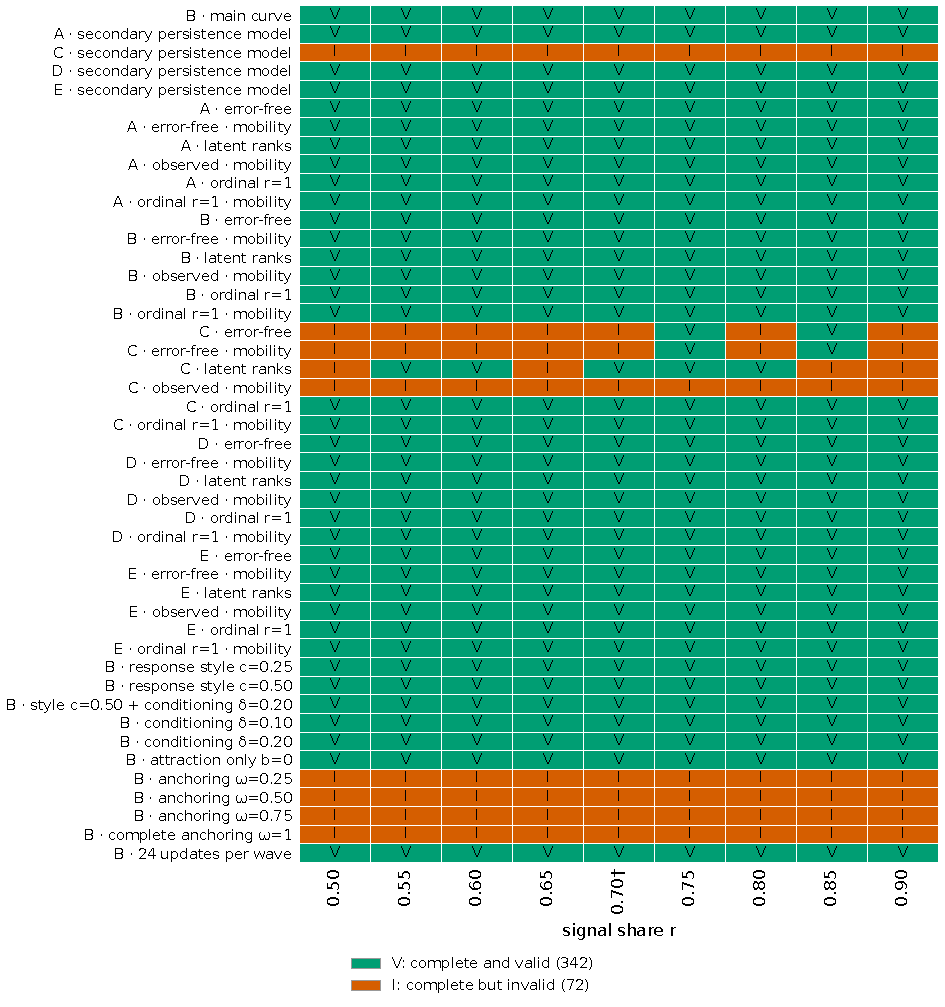
\includegraphics[width=\textwidth,height=160mm,keepaspectratio]{generated/J5_inventory_status.pdf}
\caption{Status of every unit of the prespecified inventory at the operational close, by configuration (rows) and signal share $r$. Complete and valid (V): \resultnum{v4.inv.n_valid}{342} units; Complete but invalid (I): \resultnum{v4.inv.n_invalid}{72} units; Partial at the operational close (P): \resultnum{v4.inv.n_partial}{0} units; Not started (N): \resultnum{v4.inv.n_not_started}{0} units. The legend lists only states that occur. $\dag$ $r=\resultnum{j.calibration.r}{0.70}$ was examined during calibration.}\label{fig:inventory-status}
\end{figure}



\clearpage


\section{Additional confirmatory results}\label{sec:additional}
% Additional confirmatory results (Section S6). Reorganized during the journal
% revision (agent S, 2026-10-13) from sections/supplement.tex and
% sections/results.tex of the rule-assembled attempt. Tables and figures of
% the engineering agent (generated/journal-esm-*) replace the rule-assembled
% displays when they exist; the older displays are the fallback.
\def\esmfigboundaries{fig:boundaries-by-model}%
\def\esmfigaucA{fig:auc-A}\def\esmfigaucC{fig:auc-C}\def\esmfigaucD{fig:auc-D}\def\esmfigaucE{fig:auc-E}%

The article reports the boundaries against B (Table~\ref{main-tab:boundaries-B} and Fig.~\ref{main-fig:auc-B}) and summarizes the other persistence models (Table~\ref{main-tab:other-models}). This section gives the full displays behind them, the cell values against B, the secondary targets, the gaps, the controls and sensitivities, and the diagnostics.

\subsection{Boundaries for every persistence model}\label{sec:additional-models}

Table~\ref{tab:v4-T1} gives the first and sustained boundaries for all five persistence models at every $r$, Fig.~\ref{\esmfigboundaries} plots them, and Figs.~\ref{\esmfigaucA}, \ref{\esmfigaucC}, \ref{\esmfigaucD} and~\ref{\esmfigaucE} give the AUC profiles against A, C, D and E (the profiles against B are Fig.~\ref{main-fig:auc-B} of the article).
% Moved from sections/results.tex (Other null families) of the rule-assembled attempt.
All \resultnum{v4.tab.T4.2-all-all-all.units}{36} units of the secondary persistence models finished, and \resultnum{v4.tab.T4.2-all-all-all.valid}{27} were complete and valid. The \resultnum{v4.inv.t2.n_invalid}{9} units of C were complete but invalid: their band at $a=0$ excluded \resultnum{v4.protocol.null_auc}{0.5}, with a zero-strength point AUC of \resultnum{j.models.C.zero_auc.min}{1.000} at every share, and their boundaries are suppressed. The prespecified condition for comparing persistence models required a valid main curve and all 36 secondary units complete and valid; it was not met, so no comparison across models is made, locally or for the whole curve, and no persistence model is promoted or demoted. Valid units remain displayed.
For C, the zero-strength rule is the protocol's operational eligibility rule without a guaranteed identity of the arms at zero strength, because only C's persistence arm receives the altered channel. Its failure reflects that the altered response channel alone separates the panels; by itself it establishes neither an implementation defect nor influence. Read after the results became available: because the two arms of C differ at zero strength by construction, its zero-strength check could pass only if the classifier could not see that difference, and at this panel size it could; the failure is a property of how C was designed, says nothing about persistence and, under the prespecified condition, prevented the comparison across models.
All nine units of D were complete and valid, but every first and sustained boundary against D is censored at a fit gap. The first gap is at $a=\resultnum{j.models.D.r055.first_gap}{0.10}$ at seven shares, at $a=\resultnum{j.models.D.r050.first_gap}{0.01}$ (another solver status) at $r=0.50$ and at $a=\resultnum{j.models.D.r060.first_gap}{0.003}$ (the propagation gap of amendment v4.4) at $r=0.60$. D has \resultnum{j.models.D.gaps.total}{38} gap cells: \resultnum{j.models.D.gaps.family_limit}{33} family limits on the profile, \resultnum{j.models.D.gaps.solver}{4} other solver statuses and \resultnum{j.models.D.gaps.propagation}{1} propagation gap. A family limit on the profile means that the declared profile solver reached the edge of D's parameter box ($\eta\le0.8$; Table~\ref{tab:design-conventions}) without an accepted root for the influence arm's lag-1 and lag-2 correlations. At $a=0.10$ all nine gaps of D are family limits; at $a=0.30$--0.90 the gaps include one other solver status at each of $r=0.55$, 0.70 and 0.80 (\allunitsresource\ gives the gap kinds of every unit). Read after the results became available: within its box, the declared profile solver found no admissible match for D at $a=0.10$ and 0.30 at any share, the strengths where the boundary against B lies. This is a statement about the declared matching procedure. Because the profile is checked for monotonicity only at the points it evaluates (Section~\ref{sec:dd-matching}), it does not establish that no parameter in the box reproduces those moments.
A and E were complete and valid at every share; their boundaries are displayed without a comparison with B.
The prespecified display of offsets between models applies only when the condition for comparing models is met, so it is not reported.

% Generated by ic_study.analysis.v4_report_export from the v4 report with
% manifest SHA-256 6608b3960eb73011caca97870a4ffd3dbfbcd4c2df09bbbcb576c1c9452cf981.
% Edited during the journal revision (agent S, 2026-10-13): captions, headers and
% categorical cells in plain English; every number keeps its \resultnum binding.
\begin{table*}[tp]
\caption{First and sustained boundaries at the primary target AUC 0.70 for every persistence model and signal share (the article shows the B rows in Table~\ref{main-tab:boundaries-B} and the other models in Table~\ref{main-tab:other-models}): status at the close, zero-strength check, number of gap cells, first boundary $a^*$ and sustained boundary $a_s^*$ with their boundary intervals in brackets, and the protocol's region label of $a^*$. Censored at gap $x$: the boundary, and both ends of its interval, cannot be declared across the fit gap at $a=x$ (gap-censoring rule; a sustained boundary censored at 0.9 is not a boundary at 0.9). Suppressed: no boundary because the zero-strength check failed, so the region is none. Regions follow the inherited convention: small, the whole interval within $(0,0.03]$; large, the whole interval above 0.03; indeterminate when $a^*=0$ or the interval crosses 0.03 or has a censored end; censored when the first boundary itself is censored (a label of this resource and Online Resource~2, not used in the article). The 0.03 cut is an inherited convention, not a demonstrated effect size. Grid values are printed as released (0.1 means 0.10). Models: A autoregressive; B trait plus autoregressive; C autoregressive with an altered response channel; D state-dependent; E mover--stayer. Status: CV complete and valid; CI complete but invalid. $a=0$ check: the zero-strength check. \dag\ $r=0.70$, examined during calibration. Secondary targets: Table~\ref{tab:v4-sec}; gap kinds: Tables~\ref{tab:v4-sgaps} and~\ref{tab:v4-T4}.}\label{tab:v4-T1}
\centering\scriptsize
\setlength{\tabcolsep}{2pt}
\begin{tabular}{lrllrp{2.9cm}p{2.9cm}l}
\toprule
Model & $r$ & Status & $a=0$ check & Gaps & $a^*$ [interval] & $a_s^*$ [interval] & Region \\
\midrule
B & \resultnum{v4.tab.T1.B.r050.r}{0.50} & CV & passed & \resultnum{v4.tab.T1.B.r050.gaps}{0} & \resultnum{v4.tab.T1.B.r050.a_star.1}{0.3} [\resultnum{v4.tab.T1.B.r050.a_star.2}{0.1}, \resultnum{v4.tab.T1.B.r050.a_star.3}{0.3}] & \resultnum{v4.tab.T1.B.r050.a_s_star.1}{0.3} [\resultnum{v4.tab.T1.B.r050.a_s_star.2}{0.1}, \resultnum{v4.tab.T1.B.r050.a_s_star.3}{0.3}] & large \\
B & \resultnum{v4.tab.T1.B.r055.r}{0.55} & CV & passed & \resultnum{v4.tab.T1.B.r055.gaps}{2} & \resultnum{v4.tab.T1.B.r055.a_star.1}{0.1} [\resultnum{v4.tab.T1.B.r055.a_star.2}{0.1}, \resultnum{v4.tab.T1.B.r055.a_star.3}{0.3}] & censored at gap \resultnum{v4.tab.T1.B.r055.a_s_star.1}{0.9} & large \\
B & \resultnum{v4.tab.T1.B.r060.r}{0.60} & CV & passed & \resultnum{v4.tab.T1.B.r060.gaps}{0} & \resultnum{v4.tab.T1.B.r060.a_star.1}{0.1} [\resultnum{v4.tab.T1.B.r060.a_star.2}{0.1}, \resultnum{v4.tab.T1.B.r060.a_star.3}{0.3}] & \resultnum{v4.tab.T1.B.r060.a_s_star.1}{0.1} [\resultnum{v4.tab.T1.B.r060.a_s_star.2}{0.1}, \resultnum{v4.tab.T1.B.r060.a_s_star.3}{0.3}] & large \\
B & \resultnum{v4.tab.T1.B.r065.r}{0.65} & CV & passed & \resultnum{v4.tab.T1.B.r065.gaps}{0} & \resultnum{v4.tab.T1.B.r065.a_star.1}{0.1} [\resultnum{v4.tab.T1.B.r065.a_star.2}{0.1}, \resultnum{v4.tab.T1.B.r065.a_star.3}{0.1}] & \resultnum{v4.tab.T1.B.r065.a_s_star.1}{0.1} [\resultnum{v4.tab.T1.B.r065.a_s_star.2}{0.1}, \resultnum{v4.tab.T1.B.r065.a_s_star.3}{0.1}] & large \\
B & \resultnum{v4.tab.T1.B.r070.r}{0.70}\dag{} & CV & passed & \resultnum{v4.tab.T1.B.r070.gaps}{1} & \resultnum{v4.tab.T1.B.r070.a_star.1}{0.1} [\resultnum{v4.tab.T1.B.r070.a_star.2}{0.1}, \resultnum{v4.tab.T1.B.r070.a_star.3}{0.1}] & censored at gap \resultnum{v4.tab.T1.B.r070.a_s_star.1}{0.9} & large \\
B & \resultnum{v4.tab.T1.B.r075.r}{0.75} & CV & passed & \resultnum{v4.tab.T1.B.r075.gaps}{0} & \resultnum{v4.tab.T1.B.r075.a_star.1}{0.1} [\resultnum{v4.tab.T1.B.r075.a_star.2}{0.1}, \resultnum{v4.tab.T1.B.r075.a_star.3}{0.1}] & \resultnum{v4.tab.T1.B.r075.a_s_star.1}{0.1} [\resultnum{v4.tab.T1.B.r075.a_s_star.2}{0.1}, \resultnum{v4.tab.T1.B.r075.a_s_star.3}{0.1}] & large \\
B & \resultnum{v4.tab.T1.B.r080.r}{0.80} & CV & passed & \resultnum{v4.tab.T1.B.r080.gaps}{0} & \resultnum{v4.tab.T1.B.r080.a_star.1}{0.1} [\resultnum{v4.tab.T1.B.r080.a_star.2}{0.1}, \resultnum{v4.tab.T1.B.r080.a_star.3}{0.1}] & \resultnum{v4.tab.T1.B.r080.a_s_star.1}{0.1} [\resultnum{v4.tab.T1.B.r080.a_s_star.2}{0.1}, \resultnum{v4.tab.T1.B.r080.a_s_star.3}{0.1}] & large \\
B & \resultnum{v4.tab.T1.B.r085.r}{0.85} & CV & passed & \resultnum{v4.tab.T1.B.r085.gaps}{0} & \resultnum{v4.tab.T1.B.r085.a_star.1}{0.1} [\resultnum{v4.tab.T1.B.r085.a_star.2}{0.1}, \resultnum{v4.tab.T1.B.r085.a_star.3}{0.1}] & \resultnum{v4.tab.T1.B.r085.a_s_star.1}{0.1} [\resultnum{v4.tab.T1.B.r085.a_s_star.2}{0.1}, \resultnum{v4.tab.T1.B.r085.a_s_star.3}{0.1}] & large \\
B & \resultnum{v4.tab.T1.B.r090.r}{0.90} & CV & passed & \resultnum{v4.tab.T1.B.r090.gaps}{0} & \resultnum{v4.tab.T1.B.r090.a_star.1}{0.1} [\resultnum{v4.tab.T1.B.r090.a_star.2}{0.1}, \resultnum{v4.tab.T1.B.r090.a_star.3}{0.1}] & \resultnum{v4.tab.T1.B.r090.a_s_star.1}{0.1} [\resultnum{v4.tab.T1.B.r090.a_s_star.2}{0.1}, \resultnum{v4.tab.T1.B.r090.a_s_star.3}{0.1}] & large \\
A & \resultnum{v4.tab.T1.A.r050.r}{0.50} & CV & passed & \resultnum{v4.tab.T1.A.r050.gaps}{0} & \resultnum{v4.tab.T1.A.r050.a_star.1}{0.3} [\resultnum{v4.tab.T1.A.r050.a_star.2}{0.1}, \resultnum{v4.tab.T1.A.r050.a_star.3}{0.3}] & \resultnum{v4.tab.T1.A.r050.a_s_star.1}{0.3} [\resultnum{v4.tab.T1.A.r050.a_s_star.2}{0.1}, \resultnum{v4.tab.T1.A.r050.a_s_star.3}{0.3}] & large \\
A & \resultnum{v4.tab.T1.A.r055.r}{0.55} & CV & passed & \resultnum{v4.tab.T1.A.r055.gaps}{0} & \resultnum{v4.tab.T1.A.r055.a_star.1}{0.1} [\resultnum{v4.tab.T1.A.r055.a_star.2}{0.1}, \resultnum{v4.tab.T1.A.r055.a_star.3}{0.3}] & \resultnum{v4.tab.T1.A.r055.a_s_star.1}{0.1} [\resultnum{v4.tab.T1.A.r055.a_s_star.2}{0.1}, \resultnum{v4.tab.T1.A.r055.a_s_star.3}{0.3}] & large \\
A & \resultnum{v4.tab.T1.A.r060.r}{0.60} & CV & passed & \resultnum{v4.tab.T1.A.r060.gaps}{0} & \resultnum{v4.tab.T1.A.r060.a_star.1}{0.1} [\resultnum{v4.tab.T1.A.r060.a_star.2}{0.1}, \resultnum{v4.tab.T1.A.r060.a_star.3}{0.1}] & \resultnum{v4.tab.T1.A.r060.a_s_star.1}{0.1} [\resultnum{v4.tab.T1.A.r060.a_s_star.2}{0.1}, \resultnum{v4.tab.T1.A.r060.a_s_star.3}{0.1}] & large \\
A & \resultnum{v4.tab.T1.A.r065.r}{0.65} & CV & passed & \resultnum{v4.tab.T1.A.r065.gaps}{0} & \resultnum{v4.tab.T1.A.r065.a_star.1}{0.1} [\resultnum{v4.tab.T1.A.r065.a_star.2}{0.1}, \resultnum{v4.tab.T1.A.r065.a_star.3}{0.1}] & \resultnum{v4.tab.T1.A.r065.a_s_star.1}{0.1} [\resultnum{v4.tab.T1.A.r065.a_s_star.2}{0.1}, \resultnum{v4.tab.T1.A.r065.a_s_star.3}{0.1}] & large \\
A & \resultnum{v4.tab.T1.A.r070.r}{0.70}\dag{} & CV & passed & \resultnum{v4.tab.T1.A.r070.gaps}{0} & \resultnum{v4.tab.T1.A.r070.a_star.1}{0.1} [\resultnum{v4.tab.T1.A.r070.a_star.2}{0.1}, \resultnum{v4.tab.T1.A.r070.a_star.3}{0.1}] & \resultnum{v4.tab.T1.A.r070.a_s_star.1}{0.1} [\resultnum{v4.tab.T1.A.r070.a_s_star.2}{0.1}, \resultnum{v4.tab.T1.A.r070.a_s_star.3}{0.1}] & large \\
A & \resultnum{v4.tab.T1.A.r075.r}{0.75} & CV & passed & \resultnum{v4.tab.T1.A.r075.gaps}{0} & \resultnum{v4.tab.T1.A.r075.a_star.1}{0.1} [\resultnum{v4.tab.T1.A.r075.a_star.2}{0.1}, \resultnum{v4.tab.T1.A.r075.a_star.3}{0.1}] & \resultnum{v4.tab.T1.A.r075.a_s_star.1}{0.1} [\resultnum{v4.tab.T1.A.r075.a_s_star.2}{0.1}, \resultnum{v4.tab.T1.A.r075.a_s_star.3}{0.1}] & large \\
A & \resultnum{v4.tab.T1.A.r080.r}{0.80} & CV & passed & \resultnum{v4.tab.T1.A.r080.gaps}{0} & \resultnum{v4.tab.T1.A.r080.a_star.1}{0.1} [\resultnum{v4.tab.T1.A.r080.a_star.2}{0.1}, \resultnum{v4.tab.T1.A.r080.a_star.3}{0.1}] & \resultnum{v4.tab.T1.A.r080.a_s_star.1}{0.1} [\resultnum{v4.tab.T1.A.r080.a_s_star.2}{0.1}, \resultnum{v4.tab.T1.A.r080.a_s_star.3}{0.1}] & large \\
A & \resultnum{v4.tab.T1.A.r085.r}{0.85} & CV & passed & \resultnum{v4.tab.T1.A.r085.gaps}{0} & \resultnum{v4.tab.T1.A.r085.a_star.1}{0.1} [\resultnum{v4.tab.T1.A.r085.a_star.2}{0.1}, \resultnum{v4.tab.T1.A.r085.a_star.3}{0.1}] & \resultnum{v4.tab.T1.A.r085.a_s_star.1}{0.1} [\resultnum{v4.tab.T1.A.r085.a_s_star.2}{0.1}, \resultnum{v4.tab.T1.A.r085.a_s_star.3}{0.1}] & large \\
A & \resultnum{v4.tab.T1.A.r090.r}{0.90} & CV & passed & \resultnum{v4.tab.T1.A.r090.gaps}{0} & \resultnum{v4.tab.T1.A.r090.a_star.1}{0.1} [\resultnum{v4.tab.T1.A.r090.a_star.2}{0.1}, \resultnum{v4.tab.T1.A.r090.a_star.3}{0.1}] & \resultnum{v4.tab.T1.A.r090.a_s_star.1}{0.1} [\resultnum{v4.tab.T1.A.r090.a_s_star.2}{0.1}, \resultnum{v4.tab.T1.A.r090.a_s_star.3}{0.1}] & large \\
C & \resultnum{v4.tab.T1.C.r050.r}{0.50} & CI & failed & \resultnum{v4.tab.T1.C.r050.gaps}{1} & suppressed & suppressed & none \\
C & \resultnum{v4.tab.T1.C.r055.r}{0.55} & CI & failed & \resultnum{v4.tab.T1.C.r055.gaps}{2} & suppressed & suppressed & none \\
C & \resultnum{v4.tab.T1.C.r060.r}{0.60} & CI & failed & \resultnum{v4.tab.T1.C.r060.gaps}{2} & suppressed & suppressed & none \\
C & \resultnum{v4.tab.T1.C.r065.r}{0.65} & CI & failed & \resultnum{v4.tab.T1.C.r065.gaps}{2} & suppressed & suppressed & none \\
C & \resultnum{v4.tab.T1.C.r070.r}{0.70}\dag{} & CI & failed & \resultnum{v4.tab.T1.C.r070.gaps}{3} & suppressed & suppressed & none \\
C & \resultnum{v4.tab.T1.C.r075.r}{0.75} & CI & failed & \resultnum{v4.tab.T1.C.r075.gaps}{3} & suppressed & suppressed & none \\
C & \resultnum{v4.tab.T1.C.r080.r}{0.80} & CI & failed & \resultnum{v4.tab.T1.C.r080.gaps}{3} & suppressed & suppressed & none \\
C & \resultnum{v4.tab.T1.C.r085.r}{0.85} & CI & failed & \resultnum{v4.tab.T1.C.r085.gaps}{3} & suppressed & suppressed & none \\
C & \resultnum{v4.tab.T1.C.r090.r}{0.90} & CI & failed & \resultnum{v4.tab.T1.C.r090.gaps}{3} & suppressed & suppressed & none \\
\botrule
\end{tabular}
\end{table*}
\begin{table*}[tp]
\addtocounter{table}{-\csname @ne\endcsname}
\providecommand{\theHtable}{\thetable}
\renewcommand{\theHtable}{v4-T1-part1}
\caption{First and sustained boundaries for every persistence model (continued)}\label{tab:v4-T1-part1}
\centering\scriptsize
\setlength{\tabcolsep}{2pt}
\begin{tabular}{lrllrp{2.9cm}p{2.9cm}l}
\toprule
Model & $r$ & Status & $a=0$ check & Gaps & $a^*$ [interval] & $a_s^*$ [interval] & Region \\
\midrule
D & \resultnum{v4.tab.T1.D.r050.r}{0.50} & CV & passed & \resultnum{v4.tab.T1.D.r050.gaps}{5} & censored at gap \resultnum{v4.tab.T1.D.r050.a_star.1}{0.01} & censored at gap \resultnum{v4.tab.T1.D.r050.a_s_star.1}{0.9} & censored \\
D & \resultnum{v4.tab.T1.D.r055.r}{0.55} & CV & passed & \resultnum{v4.tab.T1.D.r055.gaps}{4} & censored at gap \resultnum{v4.tab.T1.D.r055.a_star.1}{0.1} & censored at gap \resultnum{v4.tab.T1.D.r055.a_s_star.1}{0.9} & censored \\
D & \resultnum{v4.tab.T1.D.r060.r}{0.60} & CV & passed & \resultnum{v4.tab.T1.D.r060.gaps}{5} & censored at gap \resultnum{v4.tab.T1.D.r060.a_star.1}{0.003} & censored at gap \resultnum{v4.tab.T1.D.r060.a_s_star.1}{0.9} & censored \\
D & \resultnum{v4.tab.T1.D.r065.r}{0.65} & CV & passed & \resultnum{v4.tab.T1.D.r065.gaps}{4} & censored at gap \resultnum{v4.tab.T1.D.r065.a_star.1}{0.1} & censored at gap \resultnum{v4.tab.T1.D.r065.a_s_star.1}{0.9} & censored \\
D & \resultnum{v4.tab.T1.D.r070.r}{0.70}\dag{} & CV & passed & \resultnum{v4.tab.T1.D.r070.gaps}{4} & censored at gap \resultnum{v4.tab.T1.D.r070.a_star.1}{0.1} & censored at gap \resultnum{v4.tab.T1.D.r070.a_s_star.1}{0.9} & censored \\
D & \resultnum{v4.tab.T1.D.r075.r}{0.75} & CV & passed & \resultnum{v4.tab.T1.D.r075.gaps}{4} & censored at gap \resultnum{v4.tab.T1.D.r075.a_star.1}{0.1} & censored at gap \resultnum{v4.tab.T1.D.r075.a_s_star.1}{0.9} & censored \\
D & \resultnum{v4.tab.T1.D.r080.r}{0.80} & CV & passed & \resultnum{v4.tab.T1.D.r080.gaps}{4} & censored at gap \resultnum{v4.tab.T1.D.r080.a_star.1}{0.1} & censored at gap \resultnum{v4.tab.T1.D.r080.a_s_star.1}{0.9} & censored \\
D & \resultnum{v4.tab.T1.D.r085.r}{0.85} & CV & passed & \resultnum{v4.tab.T1.D.r085.gaps}{4} & censored at gap \resultnum{v4.tab.T1.D.r085.a_star.1}{0.1} & censored at gap \resultnum{v4.tab.T1.D.r085.a_s_star.1}{0.9} & censored \\
D & \resultnum{v4.tab.T1.D.r090.r}{0.90} & CV & passed & \resultnum{v4.tab.T1.D.r090.gaps}{4} & censored at gap \resultnum{v4.tab.T1.D.r090.a_star.1}{0.1} & censored at gap \resultnum{v4.tab.T1.D.r090.a_s_star.1}{0.9} & censored \\
E & \resultnum{v4.tab.T1.E.r050.r}{0.50} & CV & passed & \resultnum{v4.tab.T1.E.r050.gaps}{0} & \resultnum{v4.tab.T1.E.r050.a_star.1}{0.3} [\resultnum{v4.tab.T1.E.r050.a_star.2}{0.1}, \resultnum{v4.tab.T1.E.r050.a_star.3}{0.3}] & \resultnum{v4.tab.T1.E.r050.a_s_star.1}{0.3} [\resultnum{v4.tab.T1.E.r050.a_s_star.2}{0.1}, \resultnum{v4.tab.T1.E.r050.a_s_star.3}{0.3}] & large \\
E & \resultnum{v4.tab.T1.E.r055.r}{0.55} & CV & passed & \resultnum{v4.tab.T1.E.r055.gaps}{2} & \resultnum{v4.tab.T1.E.r055.a_star.1}{0.3} [\resultnum{v4.tab.T1.E.r055.a_star.2}{0.1}, \resultnum{v4.tab.T1.E.r055.a_star.3}{0.3}] & censored at gap \resultnum{v4.tab.T1.E.r055.a_s_star.1}{0.9} & large \\
E & \resultnum{v4.tab.T1.E.r060.r}{0.60} & CV & passed & \resultnum{v4.tab.T1.E.r060.gaps}{0} & \resultnum{v4.tab.T1.E.r060.a_star.1}{0.3} [\resultnum{v4.tab.T1.E.r060.a_star.2}{0.1}, \resultnum{v4.tab.T1.E.r060.a_star.3}{0.3}] & \resultnum{v4.tab.T1.E.r060.a_s_star.1}{0.3} [\resultnum{v4.tab.T1.E.r060.a_s_star.2}{0.1}, \resultnum{v4.tab.T1.E.r060.a_s_star.3}{0.3}] & large \\
E & \resultnum{v4.tab.T1.E.r065.r}{0.65} & CV & passed & \resultnum{v4.tab.T1.E.r065.gaps}{0} & \resultnum{v4.tab.T1.E.r065.a_star.1}{0.1} [\resultnum{v4.tab.T1.E.r065.a_star.2}{0.1}, \resultnum{v4.tab.T1.E.r065.a_star.3}{0.3}] & \resultnum{v4.tab.T1.E.r065.a_s_star.1}{0.1} [\resultnum{v4.tab.T1.E.r065.a_s_star.2}{0.1}, \resultnum{v4.tab.T1.E.r065.a_s_star.3}{0.3}] & large \\
E & \resultnum{v4.tab.T1.E.r070.r}{0.70}\dag{} & CV & passed & \resultnum{v4.tab.T1.E.r070.gaps}{1} & \resultnum{v4.tab.T1.E.r070.a_star.1}{0.1} [\resultnum{v4.tab.T1.E.r070.a_star.2}{0.1}, \resultnum{v4.tab.T1.E.r070.a_star.3}{0.3}] & censored at gap \resultnum{v4.tab.T1.E.r070.a_s_star.1}{0.9} & large \\
E & \resultnum{v4.tab.T1.E.r075.r}{0.75} & CV & passed & \resultnum{v4.tab.T1.E.r075.gaps}{0} & \resultnum{v4.tab.T1.E.r075.a_star.1}{0.1} [\resultnum{v4.tab.T1.E.r075.a_star.2}{0.1}, \resultnum{v4.tab.T1.E.r075.a_star.3}{0.3}] & \resultnum{v4.tab.T1.E.r075.a_s_star.1}{0.1} [\resultnum{v4.tab.T1.E.r075.a_s_star.2}{0.1}, \resultnum{v4.tab.T1.E.r075.a_s_star.3}{0.3}] & large \\
E & \resultnum{v4.tab.T1.E.r080.r}{0.80} & CV & passed & \resultnum{v4.tab.T1.E.r080.gaps}{0} & \resultnum{v4.tab.T1.E.r080.a_star.1}{0.1} [\resultnum{v4.tab.T1.E.r080.a_star.2}{0.1}, \resultnum{v4.tab.T1.E.r080.a_star.3}{0.1}] & \resultnum{v4.tab.T1.E.r080.a_s_star.1}{0.1} [\resultnum{v4.tab.T1.E.r080.a_s_star.2}{0.1}, \resultnum{v4.tab.T1.E.r080.a_s_star.3}{0.1}] & large \\
E & \resultnum{v4.tab.T1.E.r085.r}{0.85} & CV & passed & \resultnum{v4.tab.T1.E.r085.gaps}{0} & \resultnum{v4.tab.T1.E.r085.a_star.1}{0.1} [\resultnum{v4.tab.T1.E.r085.a_star.2}{0.1}, \resultnum{v4.tab.T1.E.r085.a_star.3}{0.1}] & \resultnum{v4.tab.T1.E.r085.a_s_star.1}{0.1} [\resultnum{v4.tab.T1.E.r085.a_s_star.2}{0.1}, \resultnum{v4.tab.T1.E.r085.a_s_star.3}{0.1}] & large \\
E & \resultnum{v4.tab.T1.E.r090.r}{0.90} & CV & passed & \resultnum{v4.tab.T1.E.r090.gaps}{0} & \resultnum{v4.tab.T1.E.r090.a_star.1}{0.1} [\resultnum{v4.tab.T1.E.r090.a_star.2}{0.1}, \resultnum{v4.tab.T1.E.r090.a_star.3}{0.1}] & \resultnum{v4.tab.T1.E.r090.a_s_star.1}{0.1} [\resultnum{v4.tab.T1.E.r090.a_s_star.2}{0.1}, \resultnum{v4.tab.T1.E.r090.a_s_star.3}{0.1}] & large \\
\botrule
\end{tabular}
\end{table*}

\begin{figure}[tp]
\centering
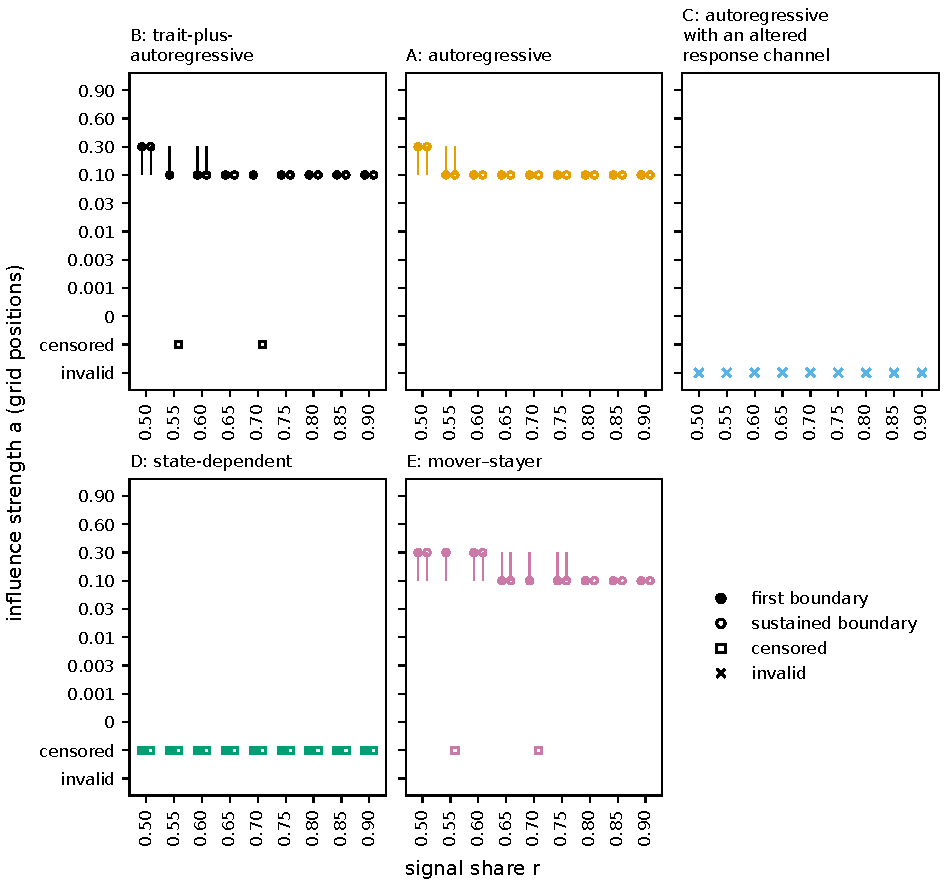
\includegraphics[width=\textwidth]{generated/J1_boundaries_by_model.pdf}
\caption{First and sustained boundaries by persistence model and signal share. Censored boundaries and invalid units occupy separate rows. Filled and open markers distinguish first and sustained boundaries.}\label{fig:boundaries-by-model}
\end{figure}

\begin{figure}[tp]
\centering
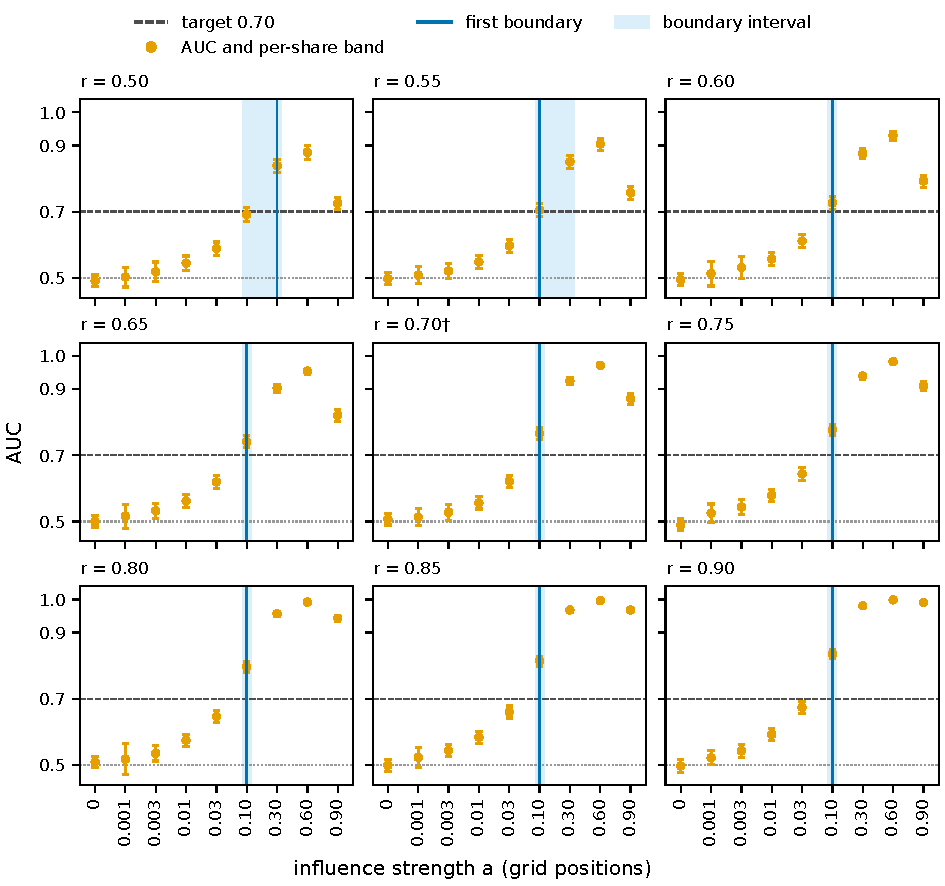
\includegraphics[width=\textwidth]{generated/J2_auc_profiles_A.pdf}
\caption{AUC profiles against autoregressive persistence (A). Vertical bars show per-share bands and crosses mark fit gaps. The target is \resultnum{j.target.r070}{0.70}. $\dag$ Examined during calibration.}\label{fig:auc-A}
\end{figure}
\begin{figure}[tp]
\centering
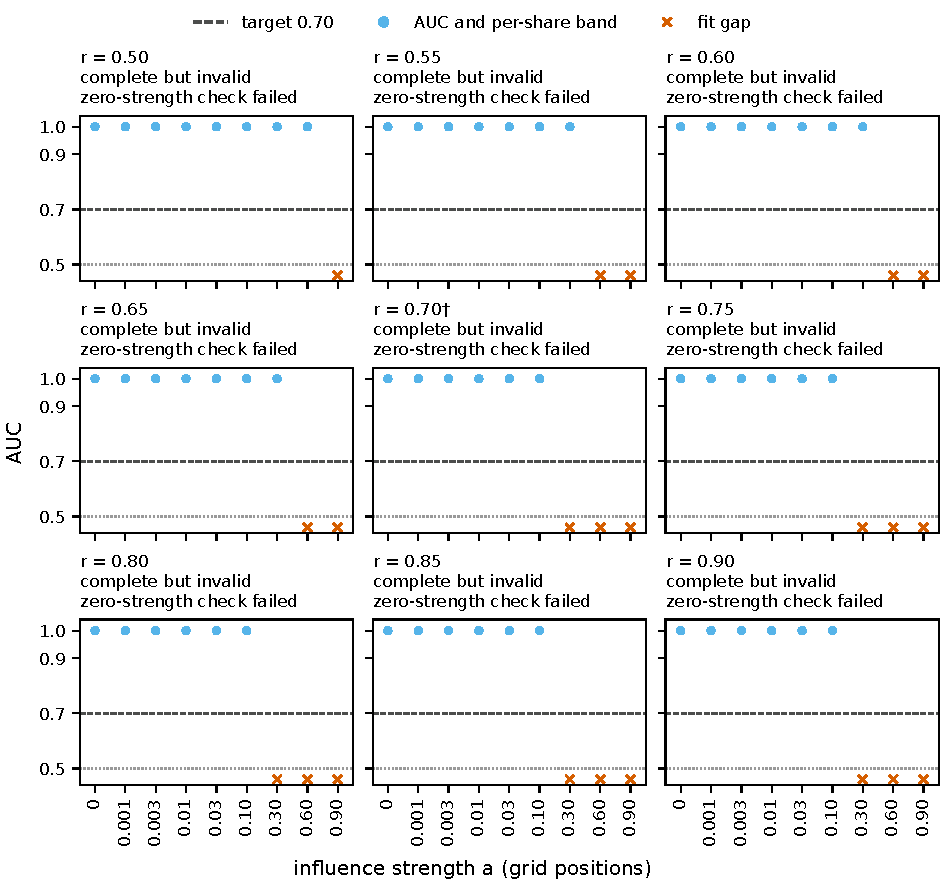
\includegraphics[width=\textwidth]{generated/J2_auc_profiles_C.pdf}
\caption{AUC profiles against autoregressive persistence with an altered response channel (C). Vertical bars show per-share bands and crosses mark fit gaps. The target is \resultnum{j.target.r070}{0.70}. $\dag$ Examined during calibration.}\label{fig:auc-C}
\end{figure}
\begin{figure}[tp]
\centering
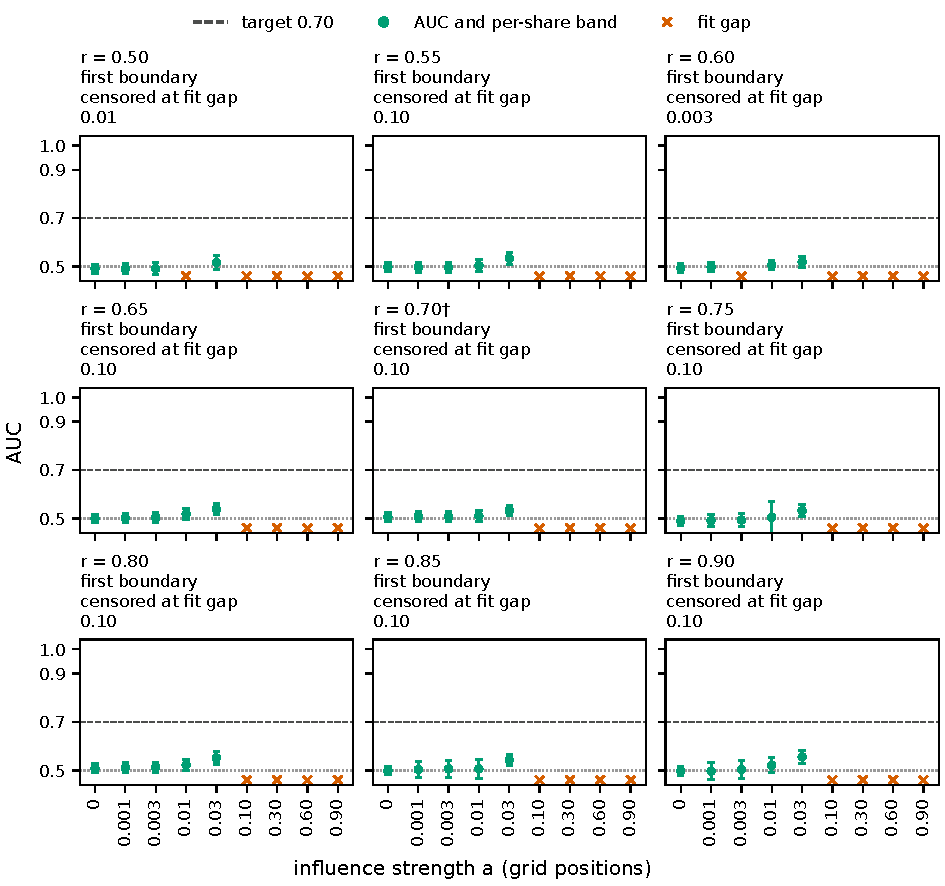
\includegraphics[width=\textwidth]{generated/J2_auc_profiles_D.pdf}
\caption{AUC profiles against state-dependent persistence (D). Vertical bars show per-share bands and crosses mark fit gaps. The target is \resultnum{j.target.r070}{0.70}. $\dag$ Examined during calibration.}\label{fig:auc-D}
\end{figure}
\begin{figure}[tp]
\centering
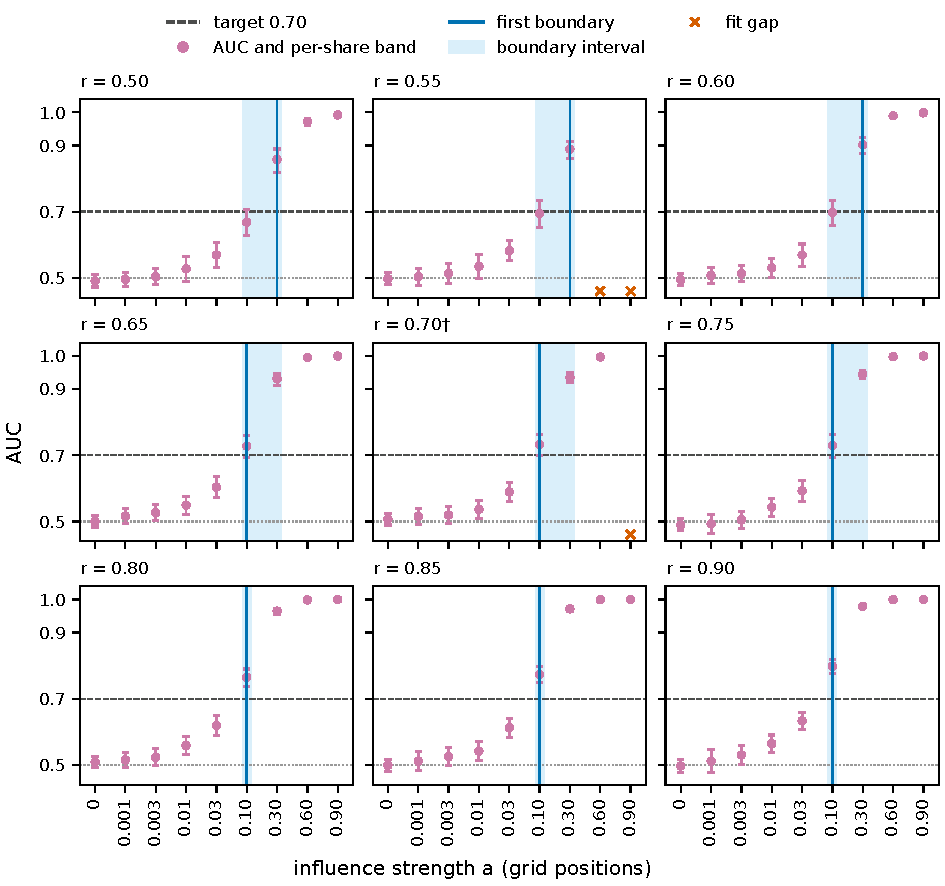
\includegraphics[width=\textwidth]{generated/J2_auc_profiles_E.pdf}
\caption{AUC profiles against mover--stayer persistence (E). Vertical bars show per-share bands and crosses mark fit gaps. The target is \resultnum{j.target.r070}{0.70}. $\dag$ Examined during calibration.}\label{fig:auc-E}
\end{figure}


% Generated by ic_study.analysis.v4_report_export from the v4 report with
% manifest SHA-256 6608b3960eb73011caca97870a4ffd3dbfbcd4c2df09bbbcb576c1c9452cf981. Export again instead of editing this file.
% MECHANISMS permission is absent, so P7 and F3 do not apply.


\subsection{Cells against B, secondary targets and low strengths}\label{sec:additional-b}

Tables~\ref{tab:b-cells}--\ref{tab:b-cells-part-c} list, for each of the 81 cells against B, the point AUC and the limits of the per-share simultaneous band, with the critical value of each share.
The score and nuisance standard errors of each cell, the fitted parameters, fit statuses and retries of the persistence model in each cell, and the mean lag correlations of each cell are absent from the released artifacts used for this resource (the public projection of the released curves and the values catalog), so they are not tabulated here; the band limits carry the combined uncertainty. Unlike these artifacts, the archived released curves hold each cell's fitted parameters, nuisance variance and fit attempts, with their statuses and retries, but not the score standard errors or mean lag correlations; the per-panel features stay in the sealed store (Section~\ref{sec:odd}, Observation). Read after the results became available: the point AUC at $a=\resultnum{j.grid.a1000}{0.10}$ rose from \resultnum{j.b.a1000.auc.min}{0.668} at $r=\resultnum{j.b.a1000.auc.min.r}{0.50}$ to \resultnum{j.b.a1000.auc.max}{0.831} at $r=\resultnum{j.b.a1000.auc.max.r}{0.90}$, and the upper band at $a=\resultnum{j.grid.a0300}{0.03}$ came closest to 0.70 at $r=\resultnum{j.b.a0300.upper.max.r}{0.90}$, where it reached \resultnum{j.b.a0300.upper.max}{0.675}, \resultnum{j.b.a0300.upper.distance_to_target}{0.025} below the target. At $a=0.03$ every lower band already lay above 0.5, while every upper band lay below 0.70 (Tables~\ref{tab:b-cells}--\ref{tab:b-cells-part-c}): the first boundary marks where the expected AUC reaches the 0.70 target, not the first strength at which the band excludes 0.5.

% Moved from sections/supplement.tex (Secondary-target boundaries) of the rule-assembled attempt.
Boundaries for the secondary targets were derived from the released bands using the same inclusive inversion and gap censoring. They were attained at \resultnum{v4.t1.sec060.n_attained}{9} values of $r$ for AUC \resultnum{v4.protocol.secondary_target.lower}{0.60} and at \resultnum{v4.t1.sec080.n_attained}{9} for AUC \resultnum{v4.protocol.secondary_target.upper}{0.80} (Table~\ref{tab:v4-sec}). At AUC 0.60 the first boundary against B was $a=\resultnum{j.b.r075.target060.point}{0.03}$ at $r=0.75$--0.90, with the interval reaching $a=\resultnum{v4.tab.T1sec.B.r090.a060.2}{0.01}$ at $r=0.90$, and $a=\resultnum{j.b.r050.target060.point}{0.10}$ at the lower shares; at AUC 0.80 it was $a=\resultnum{j.b.r050.target080.point}{0.30}$ at $r=0.50$--0.85 and $a=\resultnum{j.b.r090.target080.point}{0.10}$ at $r=0.90$. These targets are secondary and do not replace the primary target; they show that the region label of a boundary depends on the target.
The prespecified table of low-strength cells applies only when a first boundary against B lies at one of the first two positive strengths, $a=0.001$ or 0.003; none does, so it is not reported.

\begin{table}[tp]
\caption{AUC estimates and per-share bands against trait-plus-autoregressive persistence.}\label{tab:b-cells}
\centering\scriptsize
\setlength{\tabcolsep}{2pt}
\begin{tabular}{rrrrrr>{\raggedright\arraybackslash}p{34mm}}
\toprule
$r$ & $a$ & AUC & \shortstack{Lower\\band} & \shortstack{Upper\\band} & Critical & Cell state \\
\midrule
\resultnum{v4.tab.T1.B.r050.r}{0.50} & \resultnum{j.grid.a0000}{0} & \resultnum{j.b.r050.a0000.auc}{0.491} & \resultnum{j.b.r050.a0000.lower}{0.472} & \resultnum{j.b.r050.a0000.upper}{0.509} & \resultnum{j.b.r050.critical}{2.799} & available \\
\resultnum{v4.tab.T1.B.r050.r}{0.50} & \resultnum{j.grid.a0010}{0.001} & \resultnum{j.b.r050.a0010.auc}{0.498} & \resultnum{j.b.r050.a0010.lower}{0.474} & \resultnum{j.b.r050.a0010.upper}{0.523} & \resultnum{j.b.r050.critical}{2.799} & available \\
\resultnum{v4.tab.T1.B.r050.r}{0.50} & \resultnum{j.grid.a0030}{0.003} & \resultnum{j.b.r050.a0030.auc}{0.509} & \resultnum{j.b.r050.a0030.lower}{0.483} & \resultnum{j.b.r050.a0030.upper}{0.535} & \resultnum{j.b.r050.critical}{2.799} & available \\
\resultnum{v4.tab.T1.B.r050.r}{0.50} & \resultnum{j.grid.a0100}{0.01} & \resultnum{j.b.r050.a0100.auc}{0.527} & \resultnum{j.b.r050.a0100.lower}{0.496} & \resultnum{j.b.r050.a0100.upper}{0.558} & \resultnum{j.b.r050.critical}{2.799} & available \\
\resultnum{v4.tab.T1.B.r050.r}{0.50} & \resultnum{j.grid.a0300}{0.03} & \resultnum{j.b.r050.a0300.auc}{0.562} & \resultnum{j.b.r050.a0300.lower}{0.528} & \resultnum{j.b.r050.a0300.upper}{0.595} & \resultnum{j.b.r050.critical}{2.799} & available \\
\resultnum{v4.tab.T1.B.r050.r}{0.50} & \resultnum{j.grid.a1000}{0.10} & \resultnum{j.b.r050.a1000.auc}{0.668} & \resultnum{j.b.r050.a1000.lower}{0.632} & \resultnum{j.b.r050.a1000.upper}{0.703} & \resultnum{j.b.r050.critical}{2.799} & available \\
\resultnum{v4.tab.T1.B.r050.r}{0.50} & \resultnum{j.grid.a3000}{0.30} & \resultnum{j.b.r050.a3000.auc}{0.867} & \resultnum{j.b.r050.a3000.lower}{0.830} & \resultnum{j.b.r050.a3000.upper}{0.897} & \resultnum{j.b.r050.critical}{2.799} & available \\
\resultnum{v4.tab.T1.B.r050.r}{0.50} & \resultnum{j.grid.a6000}{0.60} & \resultnum{j.b.r050.a6000.auc}{0.978} & \resultnum{j.b.r050.a6000.lower}{0.968} & \resultnum{j.b.r050.a6000.upper}{0.985} & \resultnum{j.b.r050.critical}{2.799} & available \\
\resultnum{v4.tab.T1.B.r050.r}{0.50} & \resultnum{j.grid.a9000}{0.90} & \resultnum{j.b.r050.a9000.auc}{0.994} & \resultnum{j.b.r050.a9000.lower}{0.990} & \resultnum{j.b.r050.a9000.upper}{0.996} & \resultnum{j.b.r050.critical}{2.799} & available \\
\resultnum{v4.tab.T1.B.r055.r}{0.55} & \resultnum{j.grid.a0000}{0} & \resultnum{j.b.r055.a0000.auc}{0.498} & \resultnum{j.b.r055.a0000.lower}{0.480} & \resultnum{j.b.r055.a0000.upper}{0.515} & \resultnum{j.b.r055.critical}{2.773} & available \\
\resultnum{v4.tab.T1.B.r055.r}{0.55} & \resultnum{j.grid.a0010}{0.001} & \resultnum{j.b.r055.a0010.auc}{0.506} & \resultnum{j.b.r055.a0010.lower}{0.480} & \resultnum{j.b.r055.a0010.upper}{0.532} & \resultnum{j.b.r055.critical}{2.773} & available \\
\resultnum{v4.tab.T1.B.r055.r}{0.55} & \resultnum{j.grid.a0030}{0.003} & \resultnum{j.b.r055.a0030.auc}{0.517} & \resultnum{j.b.r055.a0030.lower}{0.486} & \resultnum{j.b.r055.a0030.upper}{0.548} & \resultnum{j.b.r055.critical}{2.773} & available \\
\resultnum{v4.tab.T1.B.r055.r}{0.55} & \resultnum{j.grid.a0100}{0.01} & \resultnum{j.b.r055.a0100.auc}{0.531} & \resultnum{j.b.r055.a0100.lower}{0.489} & \resultnum{j.b.r055.a0100.upper}{0.573} & \resultnum{j.b.r055.critical}{2.773} & available \\
\resultnum{v4.tab.T1.B.r055.r}{0.55} & \resultnum{j.grid.a0300}{0.03} & \resultnum{j.b.r055.a0300.auc}{0.591} & \resultnum{j.b.r055.a0300.lower}{0.561} & \resultnum{j.b.r055.a0300.upper}{0.621} & \resultnum{j.b.r055.critical}{2.773} & available \\
\resultnum{v4.tab.T1.B.r055.r}{0.55} & \resultnum{j.grid.a1000}{0.10} & \resultnum{j.b.r055.a1000.auc}{0.702} & \resultnum{j.b.r055.a1000.lower}{0.665} & \resultnum{j.b.r055.a1000.upper}{0.736} & \resultnum{j.b.r055.critical}{2.773} & available \\
\resultnum{v4.tab.T1.B.r055.r}{0.55} & \resultnum{j.grid.a3000}{0.30} & \resultnum{j.b.r055.a3000.auc}{0.900} & \resultnum{j.b.r055.a3000.lower}{0.869} & \resultnum{j.b.r055.a3000.upper}{0.924} & \resultnum{j.b.r055.critical}{2.773} & available \\
\resultnum{v4.tab.T1.B.r055.r}{0.55} & \resultnum{j.grid.a6000}{0.60} & --- & --- & --- & \resultnum{j.b.r055.critical}{2.773} & fit gap: other solver status \\
\resultnum{v4.tab.T1.B.r055.r}{0.55} & \resultnum{j.grid.a9000}{0.90} & --- & --- & --- & \resultnum{j.b.r055.critical}{2.773} & fit gap: other solver status \\
\resultnum{v4.tab.T1.B.r060.r}{0.60} & \resultnum{j.grid.a0000}{0} & \resultnum{j.b.r060.a0000.auc}{0.495} & \resultnum{j.b.r060.a0000.lower}{0.477} & \resultnum{j.b.r060.a0000.upper}{0.512} & \resultnum{j.b.r060.critical}{2.773} & available \\
\resultnum{v4.tab.T1.B.r060.r}{0.60} & \resultnum{j.grid.a0010}{0.001} & \resultnum{j.b.r060.a0010.auc}{0.498} & \resultnum{j.b.r060.a0010.lower}{0.473} & \resultnum{j.b.r060.a0010.upper}{0.524} & \resultnum{j.b.r060.critical}{2.773} & available \\
\resultnum{v4.tab.T1.B.r060.r}{0.60} & \resultnum{j.grid.a0030}{0.003} & \resultnum{j.b.r060.a0030.auc}{0.501} & \resultnum{j.b.r060.a0030.lower}{0.474} & \resultnum{j.b.r060.a0030.upper}{0.529} & \resultnum{j.b.r060.critical}{2.773} & available \\
\resultnum{v4.tab.T1.B.r060.r}{0.60} & \resultnum{j.grid.a0100}{0.01} & \resultnum{j.b.r060.a0100.auc}{0.521} & \resultnum{j.b.r060.a0100.lower}{0.487} & \resultnum{j.b.r060.a0100.upper}{0.555} & \resultnum{j.b.r060.critical}{2.773} & available \\
\resultnum{v4.tab.T1.B.r060.r}{0.60} & \resultnum{j.grid.a0300}{0.03} & \resultnum{j.b.r060.a0300.auc}{0.567} & \resultnum{j.b.r060.a0300.lower}{0.537} & \resultnum{j.b.r060.a0300.upper}{0.596} & \resultnum{j.b.r060.critical}{2.773} & available \\
\resultnum{v4.tab.T1.B.r060.r}{0.60} & \resultnum{j.grid.a1000}{0.10} & \resultnum{j.b.r060.a1000.auc}{0.702} & \resultnum{j.b.r060.a1000.lower}{0.666} & \resultnum{j.b.r060.a1000.upper}{0.736} & \resultnum{j.b.r060.critical}{2.773} & available \\
\resultnum{v4.tab.T1.B.r060.r}{0.60} & \resultnum{j.grid.a3000}{0.30} & \resultnum{j.b.r060.a3000.auc}{0.913} & \resultnum{j.b.r060.a3000.lower}{0.888} & \resultnum{j.b.r060.a3000.upper}{0.932} & \resultnum{j.b.r060.critical}{2.773} & available \\
\resultnum{v4.tab.T1.B.r060.r}{0.60} & \resultnum{j.grid.a6000}{0.60} & \resultnum{j.b.r060.a6000.auc}{0.993} & \resultnum{j.b.r060.a6000.lower}{0.989} & \resultnum{j.b.r060.a6000.upper}{0.996} & \resultnum{j.b.r060.critical}{2.773} & available \\
\resultnum{v4.tab.T1.B.r060.r}{0.60} & \resultnum{j.grid.a9000}{0.90} & \resultnum{j.b.r060.a9000.auc}{0.999} & \resultnum{j.b.r060.a9000.lower}{0.998} & \resultnum{j.b.r060.a9000.upper}{1.000} & \resultnum{j.b.r060.critical}{2.773} & available \\
\botrule
\end{tabular}
\par\smallskip\parbox{\linewidth}{$r$ is signal share in the continuous response before discretization; $a$ is influence strength. AUC is the area under the receiver operating characteristic curve. Lower and upper band are the limits of that share's band, simultaneous over strengths; Critical is the value used to form it. Available means an accepted AUC estimate exists; a fit gap means it does not. Other solver status means fitting stopped for a numerical reason. SE means standard error: score SE describes uncertainty from classification scores and nuisance SE from fitted persistence parameters. Score SE and nuisance SE are not in the released artifacts. Fitted persistence parameters, fit status and retries are absent from these public inputs. Dashes indicate unavailable quantities.}
\end{table}

\begin{table}[tp]
\caption{AUC estimates and per-share bands against trait-plus-autoregressive persistence (continued).}\label{tab:b-cells-part-b}
\centering\scriptsize
\setlength{\tabcolsep}{2pt}
\begin{tabular}{rrrrrr>{\raggedright\arraybackslash}p{34mm}}
\toprule
$r$ & $a$ & AUC & \shortstack{Lower\\band} & \shortstack{Upper\\band} & Critical & Cell state \\
\midrule
\resultnum{v4.tab.T1.B.r065.r}{0.65} & \resultnum{j.grid.a0000}{0} & \resultnum{j.b.r065.a0000.auc}{0.501} & \resultnum{j.b.r065.a0000.lower}{0.483} & \resultnum{j.b.r065.a0000.upper}{0.518} & \resultnum{j.b.r065.critical}{2.773} & available \\
\resultnum{v4.tab.T1.B.r065.r}{0.65} & \resultnum{j.grid.a0010}{0.001} & \resultnum{j.b.r065.a0010.auc}{0.516} & \resultnum{j.b.r065.a0010.lower}{0.491} & \resultnum{j.b.r065.a0010.upper}{0.541} & \resultnum{j.b.r065.critical}{2.773} & available \\
\resultnum{v4.tab.T1.B.r065.r}{0.65} & \resultnum{j.grid.a0030}{0.003} & \resultnum{j.b.r065.a0030.auc}{0.526} & \resultnum{j.b.r065.a0030.lower}{0.497} & \resultnum{j.b.r065.a0030.upper}{0.555} & \resultnum{j.b.r065.critical}{2.773} & available \\
\resultnum{v4.tab.T1.B.r065.r}{0.65} & \resultnum{j.grid.a0100}{0.01} & \resultnum{j.b.r065.a0100.auc}{0.562} & \resultnum{j.b.r065.a0100.lower}{0.534} & \resultnum{j.b.r065.a0100.upper}{0.589} & \resultnum{j.b.r065.critical}{2.773} & available \\
\resultnum{v4.tab.T1.B.r065.r}{0.65} & \resultnum{j.grid.a0300}{0.03} & \resultnum{j.b.r065.a0300.auc}{0.596} & \resultnum{j.b.r065.a0300.lower}{0.566} & \resultnum{j.b.r065.a0300.upper}{0.624} & \resultnum{j.b.r065.critical}{2.773} & available \\
\resultnum{v4.tab.T1.B.r065.r}{0.65} & \resultnum{j.grid.a1000}{0.10} & \resultnum{j.b.r065.a1000.auc}{0.740} & \resultnum{j.b.r065.a1000.lower}{0.706} & \resultnum{j.b.r065.a1000.upper}{0.771} & \resultnum{j.b.r065.critical}{2.773} & available \\
\resultnum{v4.tab.T1.B.r065.r}{0.65} & \resultnum{j.grid.a3000}{0.30} & \resultnum{j.b.r065.a3000.auc}{0.946} & \resultnum{j.b.r065.a3000.lower}{0.930} & \resultnum{j.b.r065.a3000.upper}{0.958} & \resultnum{j.b.r065.critical}{2.773} & available \\
\resultnum{v4.tab.T1.B.r065.r}{0.65} & \resultnum{j.grid.a6000}{0.60} & \resultnum{j.b.r065.a6000.auc}{0.997} & \resultnum{j.b.r065.a6000.lower}{0.995} & \resultnum{j.b.r065.a6000.upper}{0.998} & \resultnum{j.b.r065.critical}{2.773} & available \\
\resultnum{v4.tab.T1.B.r065.r}{0.65} & \resultnum{j.grid.a9000}{0.90} & \resultnum{j.b.r065.a9000.auc}{1.000} & \resultnum{j.b.r065.a9000.lower}{0.996} & \resultnum{j.b.r065.a9000.upper}{1.000} & \resultnum{j.b.r065.critical}{2.773} & available \\
\resultnum{v4.tab.T1.B.r070.r}{0.70} & \resultnum{j.grid.a0000}{0} & \resultnum{j.b.r070.a0000.auc}{0.507} & \resultnum{j.b.r070.a0000.lower}{0.489} & \resultnum{j.b.r070.a0000.upper}{0.524} & \resultnum{j.b.r070.critical}{2.773} & available \\
\resultnum{v4.tab.T1.B.r070.r}{0.70} & \resultnum{j.grid.a0010}{0.001} & \resultnum{j.b.r070.a0010.auc}{0.526} & \resultnum{j.b.r070.a0010.lower}{0.501} & \resultnum{j.b.r070.a0010.upper}{0.552} & \resultnum{j.b.r070.critical}{2.773} & available \\
\resultnum{v4.tab.T1.B.r070.r}{0.70} & \resultnum{j.grid.a0030}{0.003} & \resultnum{j.b.r070.a0030.auc}{0.524} & \resultnum{j.b.r070.a0030.lower}{0.496} & \resultnum{j.b.r070.a0030.upper}{0.552} & \resultnum{j.b.r070.critical}{2.773} & available \\
\resultnum{v4.tab.T1.B.r070.r}{0.70} & \resultnum{j.grid.a0100}{0.01} & \resultnum{j.b.r070.a0100.auc}{0.538} & \resultnum{j.b.r070.a0100.lower}{0.509} & \resultnum{j.b.r070.a0100.upper}{0.568} & \resultnum{j.b.r070.critical}{2.773} & available \\
\resultnum{v4.tab.T1.B.r070.r}{0.70} & \resultnum{j.grid.a0300}{0.03} & \resultnum{j.b.r070.a0300.auc}{0.591} & \resultnum{j.b.r070.a0300.lower}{0.559} & \resultnum{j.b.r070.a0300.upper}{0.621} & \resultnum{j.b.r070.critical}{2.773} & available \\
\resultnum{v4.tab.T1.B.r070.r}{0.70} & \resultnum{j.grid.a1000}{0.10} & \resultnum{j.b.r070.a1000.auc}{0.754} & \resultnum{j.b.r070.a1000.lower}{0.720} & \resultnum{j.b.r070.a1000.upper}{0.785} & \resultnum{j.b.r070.critical}{2.773} & available \\
\resultnum{v4.tab.T1.B.r070.r}{0.70} & \resultnum{j.grid.a3000}{0.30} & \resultnum{j.b.r070.a3000.auc}{0.950} & \resultnum{j.b.r070.a3000.lower}{0.936} & \resultnum{j.b.r070.a3000.upper}{0.962} & \resultnum{j.b.r070.critical}{2.773} & available \\
\resultnum{v4.tab.T1.B.r070.r}{0.70} & \resultnum{j.grid.a6000}{0.60} & \resultnum{j.b.r070.a6000.auc}{0.998} & \resultnum{j.b.r070.a6000.lower}{0.997} & \resultnum{j.b.r070.a6000.upper}{0.999} & \resultnum{j.b.r070.critical}{2.773} & available \\
\resultnum{v4.tab.T1.B.r070.r}{0.70} & \resultnum{j.grid.a9000}{0.90} & --- & --- & --- & \resultnum{j.b.r070.critical}{2.773} & fit gap: other solver status \\
\resultnum{v4.tab.T1.B.r075.r}{0.75} & \resultnum{j.grid.a0000}{0} & \resultnum{j.b.r075.a0000.auc}{0.490} & \resultnum{j.b.r075.a0000.lower}{0.472} & \resultnum{j.b.r075.a0000.upper}{0.507} & \resultnum{j.b.r075.critical}{2.773} & available \\
\resultnum{v4.tab.T1.B.r075.r}{0.75} & \resultnum{j.grid.a0010}{0.001} & \resultnum{j.b.r075.a0010.auc}{0.489} & \resultnum{j.b.r075.a0010.lower}{0.462} & \resultnum{j.b.r075.a0010.upper}{0.517} & \resultnum{j.b.r075.critical}{2.773} & available \\
\resultnum{v4.tab.T1.B.r075.r}{0.75} & \resultnum{j.grid.a0030}{0.003} & \resultnum{j.b.r075.a0030.auc}{0.502} & \resultnum{j.b.r075.a0030.lower}{0.472} & \resultnum{j.b.r075.a0030.upper}{0.532} & \resultnum{j.b.r075.critical}{2.773} & available \\
\resultnum{v4.tab.T1.B.r075.r}{0.75} & \resultnum{j.grid.a0100}{0.01} & \resultnum{j.b.r075.a0100.auc}{0.538} & \resultnum{j.b.r075.a0100.lower}{0.506} & \resultnum{j.b.r075.a0100.upper}{0.569} & \resultnum{j.b.r075.critical}{2.773} & available \\
\resultnum{v4.tab.T1.B.r075.r}{0.75} & \resultnum{j.grid.a0300}{0.03} & \resultnum{j.b.r075.a0300.auc}{0.600} & \resultnum{j.b.r075.a0300.lower}{0.570} & \resultnum{j.b.r075.a0300.upper}{0.630} & \resultnum{j.b.r075.critical}{2.773} & available \\
\resultnum{v4.tab.T1.B.r075.r}{0.75} & \resultnum{j.grid.a1000}{0.10} & \resultnum{j.b.r075.a1000.auc}{0.745} & \resultnum{j.b.r075.a1000.lower}{0.716} & \resultnum{j.b.r075.a1000.upper}{0.772} & \resultnum{j.b.r075.critical}{2.773} & available \\
\resultnum{v4.tab.T1.B.r075.r}{0.75} & \resultnum{j.grid.a3000}{0.30} & \resultnum{j.b.r075.a3000.auc}{0.959} & \resultnum{j.b.r075.a3000.lower}{0.948} & \resultnum{j.b.r075.a3000.upper}{0.968} & \resultnum{j.b.r075.critical}{2.773} & available \\
\resultnum{v4.tab.T1.B.r075.r}{0.75} & \resultnum{j.grid.a6000}{0.60} & \resultnum{j.b.r075.a6000.auc}{0.999} & \resultnum{j.b.r075.a6000.lower}{0.998} & \resultnum{j.b.r075.a6000.upper}{1.000} & \resultnum{j.b.r075.critical}{2.773} & available \\
\resultnum{v4.tab.T1.B.r075.r}{0.75} & \resultnum{j.grid.a9000}{0.90} & \resultnum{j.b.r075.a9000.auc}{1.000} & \resultnum{j.b.r075.a9000.lower}{0.996} & \resultnum{j.b.r075.a9000.upper}{1.000} & \resultnum{j.b.r075.critical}{2.773} & available \\
\botrule
\end{tabular}
\par\smallskip\parbox{\linewidth}{$r$ is signal share in the continuous response before discretization; $a$ is influence strength. AUC is the area under the receiver operating characteristic curve. Lower and upper band are the limits of that share's band, simultaneous over strengths; Critical is the value used to form it. Available means an accepted AUC estimate exists; a fit gap means it does not. Other solver status means fitting stopped for a numerical reason. SE means standard error: score SE describes uncertainty from classification scores and nuisance SE from fitted persistence parameters. Score SE and nuisance SE are not in the released artifacts. Fitted persistence parameters, fit status and retries are absent from these public inputs. Dashes indicate unavailable quantities.}
\end{table}

\begin{table}[tp]
\caption{AUC estimates and per-share bands against trait-plus-autoregressive persistence (continued).}\label{tab:b-cells-part-c}
\centering\scriptsize
\setlength{\tabcolsep}{2pt}
\begin{tabular}{rrrrrr>{\raggedright\arraybackslash}p{34mm}}
\toprule
$r$ & $a$ & AUC & \shortstack{Lower\\band} & \shortstack{Upper\\band} & Critical & Cell state \\
\midrule
\resultnum{v4.tab.T1.B.r080.r}{0.80} & \resultnum{j.grid.a0000}{0} & \resultnum{j.b.r080.a0000.auc}{0.509} & \resultnum{j.b.r080.a0000.lower}{0.492} & \resultnum{j.b.r080.a0000.upper}{0.526} & \resultnum{j.b.r080.critical}{2.773} & available \\
\resultnum{v4.tab.T1.B.r080.r}{0.80} & \resultnum{j.grid.a0010}{0.001} & \resultnum{j.b.r080.a0010.auc}{0.511} & \resultnum{j.b.r080.a0010.lower}{0.489} & \resultnum{j.b.r080.a0010.upper}{0.533} & \resultnum{j.b.r080.critical}{2.773} & available \\
\resultnum{v4.tab.T1.B.r080.r}{0.80} & \resultnum{j.grid.a0030}{0.003} & \resultnum{j.b.r080.a0030.auc}{0.522} & \resultnum{j.b.r080.a0030.lower}{0.495} & \resultnum{j.b.r080.a0030.upper}{0.549} & \resultnum{j.b.r080.critical}{2.773} & available \\
\resultnum{v4.tab.T1.B.r080.r}{0.80} & \resultnum{j.grid.a0100}{0.01} & \resultnum{j.b.r080.a0100.auc}{0.550} & \resultnum{j.b.r080.a0100.lower}{0.523} & \resultnum{j.b.r080.a0100.upper}{0.578} & \resultnum{j.b.r080.critical}{2.773} & available \\
\resultnum{v4.tab.T1.B.r080.r}{0.80} & \resultnum{j.grid.a0300}{0.03} & \resultnum{j.b.r080.a0300.auc}{0.611} & \resultnum{j.b.r080.a0300.lower}{0.582} & \resultnum{j.b.r080.a0300.upper}{0.640} & \resultnum{j.b.r080.critical}{2.773} & available \\
\resultnum{v4.tab.T1.B.r080.r}{0.80} & \resultnum{j.grid.a1000}{0.10} & \resultnum{j.b.r080.a1000.auc}{0.788} & \resultnum{j.b.r080.a1000.lower}{0.762} & \resultnum{j.b.r080.a1000.upper}{0.812} & \resultnum{j.b.r080.critical}{2.773} & available \\
\resultnum{v4.tab.T1.B.r080.r}{0.80} & \resultnum{j.grid.a3000}{0.30} & \resultnum{j.b.r080.a3000.auc}{0.975} & \resultnum{j.b.r080.a3000.lower}{0.967} & \resultnum{j.b.r080.a3000.upper}{0.981} & \resultnum{j.b.r080.critical}{2.773} & available \\
\resultnum{v4.tab.T1.B.r080.r}{0.80} & \resultnum{j.grid.a6000}{0.60} & \resultnum{j.b.r080.a6000.auc}{1.000} & \resultnum{j.b.r080.a6000.lower}{0.998} & \resultnum{j.b.r080.a6000.upper}{1.000} & \resultnum{j.b.r080.critical}{2.773} & available \\
\resultnum{v4.tab.T1.B.r080.r}{0.80} & \resultnum{j.grid.a9000}{0.90} & \resultnum{j.b.r080.a9000.auc}{1.000} & \resultnum{j.b.r080.a9000.lower}{0.996} & \resultnum{j.b.r080.a9000.upper}{1.000} & \resultnum{j.b.r080.critical}{2.773} & available \\
\resultnum{v4.tab.T1.B.r085.r}{0.85} & \resultnum{j.grid.a0000}{0} & \resultnum{j.b.r085.a0000.auc}{0.499} & \resultnum{j.b.r085.a0000.lower}{0.481} & \resultnum{j.b.r085.a0000.upper}{0.517} & \resultnum{j.b.r085.critical}{2.773} & available \\
\resultnum{v4.tab.T1.B.r085.r}{0.85} & \resultnum{j.grid.a0010}{0.001} & \resultnum{j.b.r085.a0010.auc}{0.514} & \resultnum{j.b.r085.a0010.lower}{0.486} & \resultnum{j.b.r085.a0010.upper}{0.542} & \resultnum{j.b.r085.critical}{2.773} & available \\
\resultnum{v4.tab.T1.B.r085.r}{0.85} & \resultnum{j.grid.a0030}{0.003} & \resultnum{j.b.r085.a0030.auc}{0.521} & \resultnum{j.b.r085.a0030.lower}{0.489} & \resultnum{j.b.r085.a0030.upper}{0.553} & \resultnum{j.b.r085.critical}{2.773} & available \\
\resultnum{v4.tab.T1.B.r085.r}{0.85} & \resultnum{j.grid.a0100}{0.01} & \resultnum{j.b.r085.a0100.auc}{0.548} & \resultnum{j.b.r085.a0100.lower}{0.522} & \resultnum{j.b.r085.a0100.upper}{0.575} & \resultnum{j.b.r085.critical}{2.773} & available \\
\resultnum{v4.tab.T1.B.r085.r}{0.85} & \resultnum{j.grid.a0300}{0.03} & \resultnum{j.b.r085.a0300.auc}{0.627} & \resultnum{j.b.r085.a0300.lower}{0.598} & \resultnum{j.b.r085.a0300.upper}{0.656} & \resultnum{j.b.r085.critical}{2.773} & available \\
\resultnum{v4.tab.T1.B.r085.r}{0.85} & \resultnum{j.grid.a1000}{0.10} & \resultnum{j.b.r085.a1000.auc}{0.797} & \resultnum{j.b.r085.a1000.lower}{0.773} & \resultnum{j.b.r085.a1000.upper}{0.820} & \resultnum{j.b.r085.critical}{2.773} & available \\
\resultnum{v4.tab.T1.B.r085.r}{0.85} & \resultnum{j.grid.a3000}{0.30} & \resultnum{j.b.r085.a3000.auc}{0.979} & \resultnum{j.b.r085.a3000.lower}{0.973} & \resultnum{j.b.r085.a3000.upper}{0.984} & \resultnum{j.b.r085.critical}{2.773} & available \\
\resultnum{v4.tab.T1.B.r085.r}{0.85} & \resultnum{j.grid.a6000}{0.60} & \resultnum{j.b.r085.a6000.auc}{1.000} & \resultnum{j.b.r085.a6000.lower}{0.996} & \resultnum{j.b.r085.a6000.upper}{1.000} & \resultnum{j.b.r085.critical}{2.773} & available \\
\resultnum{v4.tab.T1.B.r085.r}{0.85} & \resultnum{j.grid.a9000}{0.90} & \resultnum{j.b.r085.a9000.auc}{1.000} & \resultnum{j.b.r085.a9000.lower}{0.996} & \resultnum{j.b.r085.a9000.upper}{1.000} & \resultnum{j.b.r085.critical}{2.773} & available \\
\resultnum{v4.tab.T1.B.r090.r}{0.90} & \resultnum{j.grid.a0000}{0} & \resultnum{j.b.r090.a0000.auc}{0.497} & \resultnum{j.b.r090.a0000.lower}{0.479} & \resultnum{j.b.r090.a0000.upper}{0.515} & \resultnum{j.b.r090.critical}{2.773} & available \\
\resultnum{v4.tab.T1.B.r090.r}{0.90} & \resultnum{j.grid.a0010}{0.001} & \resultnum{j.b.r090.a0010.auc}{0.510} & \resultnum{j.b.r090.a0010.lower}{0.476} & \resultnum{j.b.r090.a0010.upper}{0.545} & \resultnum{j.b.r090.critical}{2.773} & available \\
\resultnum{v4.tab.T1.B.r090.r}{0.90} & \resultnum{j.grid.a0030}{0.003} & \resultnum{j.b.r090.a0030.auc}{0.529} & \resultnum{j.b.r090.a0030.lower}{0.499} & \resultnum{j.b.r090.a0030.upper}{0.560} & \resultnum{j.b.r090.critical}{2.773} & available \\
\resultnum{v4.tab.T1.B.r090.r}{0.90} & \resultnum{j.grid.a0100}{0.01} & \resultnum{j.b.r090.a0100.auc}{0.575} & \resultnum{j.b.r090.a0100.lower}{0.547} & \resultnum{j.b.r090.a0100.upper}{0.603} & \resultnum{j.b.r090.critical}{2.773} & available \\
\resultnum{v4.tab.T1.B.r090.r}{0.90} & \resultnum{j.grid.a0300}{0.03} & \resultnum{j.b.r090.a0300.auc}{0.650} & \resultnum{j.b.r090.a0300.lower}{0.625} & \resultnum{j.b.r090.a0300.upper}{0.675} & \resultnum{j.b.r090.critical}{2.773} & available \\
\resultnum{v4.tab.T1.B.r090.r}{0.90} & \resultnum{j.grid.a1000}{0.10} & \resultnum{j.b.r090.a1000.auc}{0.831} & \resultnum{j.b.r090.a1000.lower}{0.809} & \resultnum{j.b.r090.a1000.upper}{0.851} & \resultnum{j.b.r090.critical}{2.773} & available \\
\resultnum{v4.tab.T1.B.r090.r}{0.90} & \resultnum{j.grid.a3000}{0.30} & \resultnum{j.b.r090.a3000.auc}{0.990} & \resultnum{j.b.r090.a3000.lower}{0.986} & \resultnum{j.b.r090.a3000.upper}{0.992} & \resultnum{j.b.r090.critical}{2.773} & available \\
\resultnum{v4.tab.T1.B.r090.r}{0.90} & \resultnum{j.grid.a6000}{0.60} & \resultnum{j.b.r090.a6000.auc}{1.000} & \resultnum{j.b.r090.a6000.lower}{0.996} & \resultnum{j.b.r090.a6000.upper}{1.000} & \resultnum{j.b.r090.critical}{2.773} & available \\
\resultnum{v4.tab.T1.B.r090.r}{0.90} & \resultnum{j.grid.a9000}{0.90} & \resultnum{j.b.r090.a9000.auc}{1.000} & \resultnum{j.b.r090.a9000.lower}{0.996} & \resultnum{j.b.r090.a9000.upper}{1.000} & \resultnum{j.b.r090.critical}{2.773} & available \\
\botrule
\end{tabular}
\par\smallskip\parbox{\linewidth}{$r$ is signal share in the continuous response before discretization; $a$ is influence strength. AUC is the area under the receiver operating characteristic curve. Lower and upper band are the limits of that share's band, simultaneous over strengths; Critical is the value used to form it. Available means an accepted AUC estimate exists; a fit gap means it does not. Other solver status means fitting stopped for a numerical reason. SE means standard error: score SE describes uncertainty from classification scores and nuisance SE from fitted persistence parameters. Score SE and nuisance SE are not in the released artifacts. Fitted persistence parameters, fit status and retries are absent from these public inputs. Dashes indicate unavailable quantities.}
\end{table}

% Generated by ic_study.analysis.v4_report_export from the v4 report with
% manifest SHA-256 6608b3960eb73011caca97870a4ffd3dbfbcd4c2df09bbbcb576c1c9452cf981.
% Edited during the journal revision (agent S, 2026-10-13): captions, headers and
% categorical cells in plain English; every number keeps its \resultnum binding.
\begin{table*}[tp]
\caption{First boundaries against B at the secondary targets AUC 0.60 and 0.80 (prespecified), with boundary intervals in brackets, derived from the released bands by the same inclusive inversion and gap-censoring rules; the release itself reports the 0.70 boundaries only. Grid values as released (0.1 means 0.10). \dag\ $r=0.70$, examined during calibration.}\label{tab:v4-sec}
\centering\footnotesize
\setlength{\tabcolsep}{3pt}
\begin{tabular}{rp{5cm}p{5cm}}
\toprule
$r$ & $a^*$ [interval], target AUC 0.60 & $a^*$ [interval], target AUC 0.80 \\
\midrule
\resultnum{v4.tab.T1sec.B.r050.r}{0.50} & \resultnum{v4.tab.T1sec.B.r050.a060.1}{0.1} [\resultnum{v4.tab.T1sec.B.r050.a060.2}{0.1}, \resultnum{v4.tab.T1sec.B.r050.a060.3}{0.1}] & \resultnum{v4.tab.T1sec.B.r050.a080.1}{0.3} [\resultnum{v4.tab.T1sec.B.r050.a080.2}{0.3}, \resultnum{v4.tab.T1sec.B.r050.a080.3}{0.3}] \\
\resultnum{v4.tab.T1sec.B.r055.r}{0.55} & \resultnum{v4.tab.T1sec.B.r055.a060.1}{0.1} [\resultnum{v4.tab.T1sec.B.r055.a060.2}{0.03}, \resultnum{v4.tab.T1sec.B.r055.a060.3}{0.1}] & \resultnum{v4.tab.T1sec.B.r055.a080.1}{0.3} [\resultnum{v4.tab.T1sec.B.r055.a080.2}{0.3}, \resultnum{v4.tab.T1sec.B.r055.a080.3}{0.3}] \\
\resultnum{v4.tab.T1sec.B.r060.r}{0.60} & \resultnum{v4.tab.T1sec.B.r060.a060.1}{0.1} [\resultnum{v4.tab.T1sec.B.r060.a060.2}{0.1}, \resultnum{v4.tab.T1sec.B.r060.a060.3}{0.1}] & \resultnum{v4.tab.T1sec.B.r060.a080.1}{0.3} [\resultnum{v4.tab.T1sec.B.r060.a080.2}{0.3}, \resultnum{v4.tab.T1sec.B.r060.a080.3}{0.3}] \\
\resultnum{v4.tab.T1sec.B.r065.r}{0.65} & \resultnum{v4.tab.T1sec.B.r065.a060.1}{0.1} [\resultnum{v4.tab.T1sec.B.r065.a060.2}{0.03}, \resultnum{v4.tab.T1sec.B.r065.a060.3}{0.1}] & \resultnum{v4.tab.T1sec.B.r065.a080.1}{0.3} [\resultnum{v4.tab.T1sec.B.r065.a080.2}{0.3}, \resultnum{v4.tab.T1sec.B.r065.a080.3}{0.3}] \\
\resultnum{v4.tab.T1sec.B.r070.r}{0.70}\dag{} & \resultnum{v4.tab.T1sec.B.r070.a060.1}{0.1} [\resultnum{v4.tab.T1sec.B.r070.a060.2}{0.03}, \resultnum{v4.tab.T1sec.B.r070.a060.3}{0.1}] & \resultnum{v4.tab.T1sec.B.r070.a080.1}{0.3} [\resultnum{v4.tab.T1sec.B.r070.a080.2}{0.3}, \resultnum{v4.tab.T1sec.B.r070.a080.3}{0.3}] \\
\resultnum{v4.tab.T1sec.B.r075.r}{0.75} & \resultnum{v4.tab.T1sec.B.r075.a060.1}{0.03} [\resultnum{v4.tab.T1sec.B.r075.a060.2}{0.03}, \resultnum{v4.tab.T1sec.B.r075.a060.3}{0.1}] & \resultnum{v4.tab.T1sec.B.r075.a080.1}{0.3} [\resultnum{v4.tab.T1sec.B.r075.a080.2}{0.3}, \resultnum{v4.tab.T1sec.B.r075.a080.3}{0.3}] \\
\resultnum{v4.tab.T1sec.B.r080.r}{0.80} & \resultnum{v4.tab.T1sec.B.r080.a060.1}{0.03} [\resultnum{v4.tab.T1sec.B.r080.a060.2}{0.03}, \resultnum{v4.tab.T1sec.B.r080.a060.3}{0.1}] & \resultnum{v4.tab.T1sec.B.r080.a080.1}{0.3} [\resultnum{v4.tab.T1sec.B.r080.a080.2}{0.1}, \resultnum{v4.tab.T1sec.B.r080.a080.3}{0.3}] \\
\resultnum{v4.tab.T1sec.B.r085.r}{0.85} & \resultnum{v4.tab.T1sec.B.r085.a060.1}{0.03} [\resultnum{v4.tab.T1sec.B.r085.a060.2}{0.03}, \resultnum{v4.tab.T1sec.B.r085.a060.3}{0.1}] & \resultnum{v4.tab.T1sec.B.r085.a080.1}{0.3} [\resultnum{v4.tab.T1sec.B.r085.a080.2}{0.1}, \resultnum{v4.tab.T1sec.B.r085.a080.3}{0.3}] \\
\resultnum{v4.tab.T1sec.B.r090.r}{0.90} & \resultnum{v4.tab.T1sec.B.r090.a060.1}{0.03} [\resultnum{v4.tab.T1sec.B.r090.a060.2}{0.01}, \resultnum{v4.tab.T1sec.B.r090.a060.3}{0.03}] & \resultnum{v4.tab.T1sec.B.r090.a080.1}{0.1} [\resultnum{v4.tab.T1sec.B.r090.a080.2}{0.1}, \resultnum{v4.tab.T1sec.B.r090.a080.3}{0.1}] \\
\botrule
\end{tabular}
\end{table*}

% Generated by ic_study.analysis.v4_report_export from the v4 report with
% manifest SHA-256 6608b3960eb73011caca97870a4ffd3dbfbcd4c2df09bbbcb576c1c9452cf981. Export again instead of editing this file.
% No first boundary against B lies at the first two positive strengths, so branch B04 and this table do not apply.


\subsection{Gaps, eligible domain and diagnostics}\label{sec:additional-diagnostics}

% Moved from sections/results.tex (Boundaries against B; Diagnostics and descriptive scope).
The curves against B contain \resultnum{v4.t1.gap_cells}{3} gap cells in \resultnum{v4.t1.n_gap_units}{2} units. Gap-status counts were: screened without a persistence-model evaluation, \resultnum{v4.t1.gap.screened}{0}; family limit along the profile, \resultnum{v4.t1.gap.profile_limit}{0}; other solver status, \resultnum{v4.t1.gap.solver}{3}; and validation failure in both attempts, \resultnum{v4.t1.gap.validation}{0} cells (Table~\ref{tab:v4-sgaps}). No gap is counted as an AUC below the target or as evidence that separation is impossible.
Boundaries are computed on the available strengths and are not declared across a gap. The release records \resultnum{v4.t1.n_first_gap}{0} first boundaries and \resultnum{v4.t1.n_sustained_gap}{2} sustained boundaries against B as censored, with the strength of the gap stated for each. At $r=0.55$ fits failed at $a=0.60$ and 0.90, and at $r=0.70$ at $a=0.90$; no strength lies above the last gap, so the sustained boundary is censored by construction, while at every available strength above the first boundary the lower band exceeded 0.70 (Tables~\ref{tab:b-cells}--\ref{tab:b-cells-part-c}). Where a sustained boundary is censored at a gap, it is declared only above the last gap and only when every higher strength is available, so a sustained boundary that lies below the last gap is censored rather than moved above it. A sustained boundary declared at the first strength above the last gap is kept although the unobserved gap strength could also have met the target, so such a boundary is an upper bound; no curve against B is in that case. First and sustained boundaries are therefore equal at seven shares and the sustained boundary is gap-censored at two; the censoring reflects the fit gaps, not an observed fall of the AUC below the target.
For every $r$, Table~\ref{tab:v4-sgaps} lists the eligible domain: the strengths not excluded by the feasibility screen. This makes explicit the part of the grid on which a boundary can be obtained.

The boundary interval of $a^*$ spanned at most one grid step at all \resultnum{v4.t1.n_attained}{9} shares where $a^*$ was attained; one step can be a factor of three (from 0.10 to 0.30). This meets the frozen precision target, which is a planning goal rather than a statement of power. At \resultnum{v4.t1.n_crossing}{9} values of $r$ the lower band exceeded \resultnum{v4.protocol.target}{0.70} at some strength; ``crossing'' refers only to such strengths.
The band-monotonicity flag, which marks any decrease between consecutive lower or upper band limits, is raised for \resultnum{v4.t1.n_nonmonotone_band}{5} of the nine curves against B. This diagnostic concerns band endpoints, not a dip of the point estimate or a difference between first and sustained boundaries. Neither the solver nor the band enforces monotonicity in $a$, and the release does not identify the source of a reversal.
The empirical max-$t$ critical value exceeded the \resultnum{v4.protocol.critical_floor}{2.7729} floor in \resultnum{v4.all.n_exceeds_floor}{64} of the \resultnum{v4.all.n_curves}{414} released curves, including \resultnum{v4.t1.n_exceeds_floor}{1} of the curves against B; these bands use the empirical critical value. In the other curves the critical value is the floor, the normal Bonferroni value for nine strengths; their bands are approximate simultaneous bands with that floor, not distribution-free Bonferroni bands (Section~\ref{sec:dd-band}). The covariance-Jacobian flags of the dispersion check are reported in Section~\ref{sec:record-gate}.
Statements about how $a^*$ varies across $r$ are descriptive: the bands are simultaneous within each $r$ only, seeds differ across $r$, and no simultaneous band over all \resultnum{v4.protocol.grid_cells}{81} cells was prespecified. The nine-share result is a conjunction without a joint error rate. The unit at $r=\resultnum{v4.protocol.r.070}{0.70}$ was examined during calibration and is marked in every figure and table; it remains part of the whole curve, alongside the other eight values, and is not interpreted on its own.

% Generated by ic_study.analysis.v4_report_export from the v4 report with
% manifest SHA-256 6608b3960eb73011caca97870a4ffd3dbfbcd4c2df09bbbcb576c1c9452cf981.
% Edited during the journal revision (agent S, 2026-10-13): captions, headers and
% categorical cells in plain English; every number keeps its \resultnum binding.
\begin{table*}[tp]
\caption{Eligible domain of the nine B units: the strengths not excluded by the feasibility screen (all nine at every $r$), and the gap cells by kind: family limit at the screen (no solver evaluation), family limit on the profile, other solver status, and accepted fit that failed validation in both attempts. Grid values as released.}\label{tab:v4-sgaps}
\centering\footnotesize
\setlength{\tabcolsep}{3pt}
\begin{tabular}{rp{1.9cm}p{4.6cm}rrrr}
\toprule
$r$ & Status & Strengths not excluded by the screen & screened & profile limit & solver & validation \\
\midrule
\resultnum{v4.tab.Sgaps.B.r050.r}{0.50} & complete and valid & \resultnum{v4.tab.Sgaps.B.r050.eligible.1}{0}, \resultnum{v4.tab.Sgaps.B.r050.eligible.2}{0.001}, \resultnum{v4.tab.Sgaps.B.r050.eligible.3}{0.003}, \resultnum{v4.tab.Sgaps.B.r050.eligible.4}{0.01}, \resultnum{v4.tab.Sgaps.B.r050.eligible.5}{0.03}, \resultnum{v4.tab.Sgaps.B.r050.eligible.6}{0.1}, \resultnum{v4.tab.Sgaps.B.r050.eligible.7}{0.3}, \resultnum{v4.tab.Sgaps.B.r050.eligible.8}{0.6}, \resultnum{v4.tab.Sgaps.B.r050.eligible.9}{0.9} & \resultnum{v4.tab.Sgaps.B.r050.screened}{0} & \resultnum{v4.tab.Sgaps.B.r050.family_limit}{0} & \resultnum{v4.tab.Sgaps.B.r050.solver}{0} & \resultnum{v4.tab.Sgaps.B.r050.validation}{0} \\
\resultnum{v4.tab.Sgaps.B.r055.r}{0.55} & complete and valid & \resultnum{v4.tab.Sgaps.B.r055.eligible.1}{0}, \resultnum{v4.tab.Sgaps.B.r055.eligible.2}{0.001}, \resultnum{v4.tab.Sgaps.B.r055.eligible.3}{0.003}, \resultnum{v4.tab.Sgaps.B.r055.eligible.4}{0.01}, \resultnum{v4.tab.Sgaps.B.r055.eligible.5}{0.03}, \resultnum{v4.tab.Sgaps.B.r055.eligible.6}{0.1}, \resultnum{v4.tab.Sgaps.B.r055.eligible.7}{0.3}, \resultnum{v4.tab.Sgaps.B.r055.eligible.8}{0.6}, \resultnum{v4.tab.Sgaps.B.r055.eligible.9}{0.9} & \resultnum{v4.tab.Sgaps.B.r055.screened}{0} & \resultnum{v4.tab.Sgaps.B.r055.family_limit}{0} & \resultnum{v4.tab.Sgaps.B.r055.solver}{2} & \resultnum{v4.tab.Sgaps.B.r055.validation}{0} \\
\resultnum{v4.tab.Sgaps.B.r060.r}{0.60} & complete and valid & \resultnum{v4.tab.Sgaps.B.r060.eligible.1}{0}, \resultnum{v4.tab.Sgaps.B.r060.eligible.2}{0.001}, \resultnum{v4.tab.Sgaps.B.r060.eligible.3}{0.003}, \resultnum{v4.tab.Sgaps.B.r060.eligible.4}{0.01}, \resultnum{v4.tab.Sgaps.B.r060.eligible.5}{0.03}, \resultnum{v4.tab.Sgaps.B.r060.eligible.6}{0.1}, \resultnum{v4.tab.Sgaps.B.r060.eligible.7}{0.3}, \resultnum{v4.tab.Sgaps.B.r060.eligible.8}{0.6}, \resultnum{v4.tab.Sgaps.B.r060.eligible.9}{0.9} & \resultnum{v4.tab.Sgaps.B.r060.screened}{0} & \resultnum{v4.tab.Sgaps.B.r060.family_limit}{0} & \resultnum{v4.tab.Sgaps.B.r060.solver}{0} & \resultnum{v4.tab.Sgaps.B.r060.validation}{0} \\
\resultnum{v4.tab.Sgaps.B.r065.r}{0.65} & complete and valid & \resultnum{v4.tab.Sgaps.B.r065.eligible.1}{0}, \resultnum{v4.tab.Sgaps.B.r065.eligible.2}{0.001}, \resultnum{v4.tab.Sgaps.B.r065.eligible.3}{0.003}, \resultnum{v4.tab.Sgaps.B.r065.eligible.4}{0.01}, \resultnum{v4.tab.Sgaps.B.r065.eligible.5}{0.03}, \resultnum{v4.tab.Sgaps.B.r065.eligible.6}{0.1}, \resultnum{v4.tab.Sgaps.B.r065.eligible.7}{0.3}, \resultnum{v4.tab.Sgaps.B.r065.eligible.8}{0.6}, \resultnum{v4.tab.Sgaps.B.r065.eligible.9}{0.9} & \resultnum{v4.tab.Sgaps.B.r065.screened}{0} & \resultnum{v4.tab.Sgaps.B.r065.family_limit}{0} & \resultnum{v4.tab.Sgaps.B.r065.solver}{0} & \resultnum{v4.tab.Sgaps.B.r065.validation}{0} \\
\resultnum{v4.tab.Sgaps.B.r070.r}{0.70} & complete and valid & \resultnum{v4.tab.Sgaps.B.r070.eligible.1}{0}, \resultnum{v4.tab.Sgaps.B.r070.eligible.2}{0.001}, \resultnum{v4.tab.Sgaps.B.r070.eligible.3}{0.003}, \resultnum{v4.tab.Sgaps.B.r070.eligible.4}{0.01}, \resultnum{v4.tab.Sgaps.B.r070.eligible.5}{0.03}, \resultnum{v4.tab.Sgaps.B.r070.eligible.6}{0.1}, \resultnum{v4.tab.Sgaps.B.r070.eligible.7}{0.3}, \resultnum{v4.tab.Sgaps.B.r070.eligible.8}{0.6}, \resultnum{v4.tab.Sgaps.B.r070.eligible.9}{0.9} & \resultnum{v4.tab.Sgaps.B.r070.screened}{0} & \resultnum{v4.tab.Sgaps.B.r070.family_limit}{0} & \resultnum{v4.tab.Sgaps.B.r070.solver}{1} & \resultnum{v4.tab.Sgaps.B.r070.validation}{0} \\
\resultnum{v4.tab.Sgaps.B.r075.r}{0.75} & complete and valid & \resultnum{v4.tab.Sgaps.B.r075.eligible.1}{0}, \resultnum{v4.tab.Sgaps.B.r075.eligible.2}{0.001}, \resultnum{v4.tab.Sgaps.B.r075.eligible.3}{0.003}, \resultnum{v4.tab.Sgaps.B.r075.eligible.4}{0.01}, \resultnum{v4.tab.Sgaps.B.r075.eligible.5}{0.03}, \resultnum{v4.tab.Sgaps.B.r075.eligible.6}{0.1}, \resultnum{v4.tab.Sgaps.B.r075.eligible.7}{0.3}, \resultnum{v4.tab.Sgaps.B.r075.eligible.8}{0.6}, \resultnum{v4.tab.Sgaps.B.r075.eligible.9}{0.9} & \resultnum{v4.tab.Sgaps.B.r075.screened}{0} & \resultnum{v4.tab.Sgaps.B.r075.family_limit}{0} & \resultnum{v4.tab.Sgaps.B.r075.solver}{0} & \resultnum{v4.tab.Sgaps.B.r075.validation}{0} \\
\resultnum{v4.tab.Sgaps.B.r080.r}{0.80} & complete and valid & \resultnum{v4.tab.Sgaps.B.r080.eligible.1}{0}, \resultnum{v4.tab.Sgaps.B.r080.eligible.2}{0.001}, \resultnum{v4.tab.Sgaps.B.r080.eligible.3}{0.003}, \resultnum{v4.tab.Sgaps.B.r080.eligible.4}{0.01}, \resultnum{v4.tab.Sgaps.B.r080.eligible.5}{0.03}, \resultnum{v4.tab.Sgaps.B.r080.eligible.6}{0.1}, \resultnum{v4.tab.Sgaps.B.r080.eligible.7}{0.3}, \resultnum{v4.tab.Sgaps.B.r080.eligible.8}{0.6}, \resultnum{v4.tab.Sgaps.B.r080.eligible.9}{0.9} & \resultnum{v4.tab.Sgaps.B.r080.screened}{0} & \resultnum{v4.tab.Sgaps.B.r080.family_limit}{0} & \resultnum{v4.tab.Sgaps.B.r080.solver}{0} & \resultnum{v4.tab.Sgaps.B.r080.validation}{0} \\
\resultnum{v4.tab.Sgaps.B.r085.r}{0.85} & complete and valid & \resultnum{v4.tab.Sgaps.B.r085.eligible.1}{0}, \resultnum{v4.tab.Sgaps.B.r085.eligible.2}{0.001}, \resultnum{v4.tab.Sgaps.B.r085.eligible.3}{0.003}, \resultnum{v4.tab.Sgaps.B.r085.eligible.4}{0.01}, \resultnum{v4.tab.Sgaps.B.r085.eligible.5}{0.03}, \resultnum{v4.tab.Sgaps.B.r085.eligible.6}{0.1}, \resultnum{v4.tab.Sgaps.B.r085.eligible.7}{0.3}, \resultnum{v4.tab.Sgaps.B.r085.eligible.8}{0.6}, \resultnum{v4.tab.Sgaps.B.r085.eligible.9}{0.9} & \resultnum{v4.tab.Sgaps.B.r085.screened}{0} & \resultnum{v4.tab.Sgaps.B.r085.family_limit}{0} & \resultnum{v4.tab.Sgaps.B.r085.solver}{0} & \resultnum{v4.tab.Sgaps.B.r085.validation}{0} \\
\resultnum{v4.tab.Sgaps.B.r090.r}{0.90} & complete and valid & \resultnum{v4.tab.Sgaps.B.r090.eligible.1}{0}, \resultnum{v4.tab.Sgaps.B.r090.eligible.2}{0.001}, \resultnum{v4.tab.Sgaps.B.r090.eligible.3}{0.003}, \resultnum{v4.tab.Sgaps.B.r090.eligible.4}{0.01}, \resultnum{v4.tab.Sgaps.B.r090.eligible.5}{0.03}, \resultnum{v4.tab.Sgaps.B.r090.eligible.6}{0.1}, \resultnum{v4.tab.Sgaps.B.r090.eligible.7}{0.3}, \resultnum{v4.tab.Sgaps.B.r090.eligible.8}{0.6}, \resultnum{v4.tab.Sgaps.B.r090.eligible.9}{0.9} & \resultnum{v4.tab.Sgaps.B.r090.screened}{0} & \resultnum{v4.tab.Sgaps.B.r090.family_limit}{0} & \resultnum{v4.tab.Sgaps.B.r090.solver}{0} & \resultnum{v4.tab.Sgaps.B.r090.validation}{0} \\
\botrule
\end{tabular}
\end{table*}


\subsection{Measurement controls and sensitivities}\label{sec:additional-controls}

% Moved from sections/results.tex (Controls and sensitivities) of the rule-assembled attempt.
The measurement-control tier ended with \resultnum{v4.inv.t3.n_valid}{243} of its \resultnum{v4.protocol.units.t3}{270} units complete and valid, and \resultnum{v4.inv.t3.n_incomplete}{0} not started or partial (Table~\ref{tab:v4-T4}). Table~\ref{tab:controls} gives the first boundaries of the three controls against B: the error-free latent control reached the target at $a=\resultnum{j.grid.a0300}{0.03}$ at \resultnum{j.controls.latent.n_boundary_a0300}{8} shares, \resultnum{j.controls.latent.n_small}{5} of them in the small region, while the ordinal control with $r=1$ and the latent-rank control reached it at $a=0.10$ at every share. The controls hold $\eta$ at the value fitted on the observed channel.
At \resultnum{v4.t3.n_obs_exceeds}{30} of the \resultnum{v4.t3.n_pairs_compared}{36} model-and-$r$ pairs with a valid observed unit and at least one valid control, the observed-channel point AUC exceeded the latent, ordinal ($r=1$) or latent-rank control at some strength available in both units (\allunitsresource). Under the frozen rule, this is read as sensitivity of the lag statistics to the response transformation and to the rematched persistence parameters, not as information created by response error. Read after the results became available, the count carries little information: it asks whether an excess occurs at any of up to nine strengths, several with AUCs near 0.5, where an excess arises by chance, and the controls hold $\eta$ at the observed fit.
For \resultnum{v4.t3.n_channel_not_assessed}{13} pairs with a valid observed unit, channel dependence was not assessed because at least one control was invalid, absent or had a gap. Mobility summaries are reported separately (\allunitsresource) and do not add support to the lag-decay comparison.

In the sensitivity tiers, \resultnum{v4.inv.t4.n_valid}{45} of \resultnum{v4.protocol.units.t4}{45} response-channel units and \resultnum{v4.inv.t5.n_valid}{9} of \resultnum{v4.protocol.units.t5}{45} mechanism units were complete and valid. Of the \resultnum{v4.protocol.units.t6}{9} units with \resultnum{v4.protocol.steps}{24} update steps per wave, \resultnum{v4.inv.t6.n_valid}{9} were complete and valid. A sensitivity unit is one sensitivity scenario at one $r$. Each of the \resultnum{v4.sens.n_pairs_compared}{63} sensitivity units that were complete and valid can be compared with the main B unit at the same $r$, which was complete and valid at every share. In \resultnum{v4.sens.n_region_differs}{8} of them, the sensitivity assigned $a^*$ to a different region from the main B unit (Table~\ref{tab:sensitivity-differences}): panel conditioning ($\delta=0.10$) at $r=\resultnum{j.sensitivity.d010.r055.r}{0.55}$, where the sensitivity boundary is censored at a fit gap at $a=\resultnum{j.sensitivity.d010.r055.sensitivity.gap.0.a}{0.001}$; attraction only ($b=0$) at $r=\resultnum{j.sensitivity.b000.r080.r}{0.80}$, \resultnum{j.sensitivity.b000.r085.r}{0.85} and \resultnum{j.sensitivity.b000.r090.r}{0.90}, where the interval reaches $a=0.03$ (point $a=\resultnum{j.sensitivity.b000.r090.sensitivity.point}{0.03}$ at $r=0.90$), so the region is indeterminate; and 24 update steps per wave at $r=0.50$, 0.60, 0.65 and 0.85. These differences are reported without reweighting or replacing the main result, and no sensitivity is promoted to a primary analysis. All pairs are in \allunitsresource.
The response-style and conditioning scenarios vary one factor at a time, and their combination is an identified exploratory analysis. Under complete anchoring ($\omega=\resultnum{v4.protocol.omega_full}{1}$), the latent waves repeat the initial wave regardless of $a$; these units therefore check that degeneracy and provide no information about $a$ (Section~\ref{sec:inventory}). The \resultnum{v4.protocol.steps}{24}-step scenario retains the per-step coefficients, which lowers annual latent persistence overall; its units therefore describe a changed process rather than the main process at a finer time resolution.

\begin{table}[tp]
\caption{Measurement-control boundaries against trait-plus-autoregressive persistence.}\label{tab:controls}
\centering\scriptsize
\setlength{\tabcolsep}{2pt}
\begin{tabular}{l>{\raggedright\arraybackslash}p{29mm}l>{\raggedright\arraybackslash}p{29mm}>{\raggedright\arraybackslash}p{29mm}}
\toprule
Design $r$ & Latent [interval] & Latent region & Ordinal [interval] & Latent rank [interval] \\
\midrule
\resultnum{j.controls.latent.r050.r}{0.50} & \resultnum{j.controls.latent.r050.first.point}{0.10} [\resultnum{j.controls.latent.r050.first.lower}{0.03}, \resultnum{j.controls.latent.r050.first.upper}{0.10}] & indeterminate & \resultnum{j.controls.ordinal_one.r050.first.point}{0.10} [\resultnum{j.controls.ordinal_one.r050.first.lower}{0.10}, \resultnum{j.controls.ordinal_one.r050.first.upper}{0.10}] & \resultnum{j.controls.latent_rank.r050.first.point}{0.10} [\resultnum{j.controls.latent_rank.r050.first.lower}{0.10}, \resultnum{j.controls.latent_rank.r050.first.upper}{0.10}] \\
\resultnum{j.controls.latent.r055.r}{0.55} & \resultnum{j.controls.latent.r055.first.point}{0.03} [\resultnum{j.controls.latent.r055.first.lower}{0.03}, \resultnum{j.controls.latent.r055.first.upper}{0.03}] & small & \resultnum{j.controls.ordinal_one.r055.first.point}{0.10} [\resultnum{j.controls.ordinal_one.r055.first.lower}{0.10}, \resultnum{j.controls.ordinal_one.r055.first.upper}{0.10}] & \resultnum{j.controls.latent_rank.r055.first.point}{0.10} [\resultnum{j.controls.latent_rank.r055.first.lower}{0.10}, \resultnum{j.controls.latent_rank.r055.first.upper}{0.10}] \\
\resultnum{j.controls.latent.r060.r}{0.60} & \resultnum{j.controls.latent.r060.first.point}{0.03} [\resultnum{j.controls.latent.r060.first.lower}{0.03}, \resultnum{j.controls.latent.r060.first.upper}{0.10}] & indeterminate & \resultnum{j.controls.ordinal_one.r060.first.point}{0.10} [\resultnum{j.controls.ordinal_one.r060.first.lower}{0.10}, \resultnum{j.controls.ordinal_one.r060.first.upper}{0.10}] & \resultnum{j.controls.latent_rank.r060.first.point}{0.10} [\resultnum{j.controls.latent_rank.r060.first.lower}{0.10}, \resultnum{j.controls.latent_rank.r060.first.upper}{0.10}] \\
\resultnum{j.controls.latent.r065.r}{0.65} & \resultnum{j.controls.latent.r065.first.point}{0.03} [\resultnum{j.controls.latent.r065.first.lower}{0.03}, \resultnum{j.controls.latent.r065.first.upper}{0.10}] & indeterminate & \resultnum{j.controls.ordinal_one.r065.first.point}{0.10} [\resultnum{j.controls.ordinal_one.r065.first.lower}{0.10}, \resultnum{j.controls.ordinal_one.r065.first.upper}{0.10}] & \resultnum{j.controls.latent_rank.r065.first.point}{0.10} [\resultnum{j.controls.latent_rank.r065.first.lower}{0.10}, \resultnum{j.controls.latent_rank.r065.first.upper}{0.10}] \\
\resultnum{j.controls.latent.r070.r}{0.70} & \resultnum{j.controls.latent.r070.first.point}{0.03} [\resultnum{j.controls.latent.r070.first.lower}{0.03}, \resultnum{j.controls.latent.r070.first.upper}{0.10}] & indeterminate & \resultnum{j.controls.ordinal_one.r070.first.point}{0.10} [\resultnum{j.controls.ordinal_one.r070.first.lower}{0.10}, \resultnum{j.controls.ordinal_one.r070.first.upper}{0.10}] & \resultnum{j.controls.latent_rank.r070.first.point}{0.10} [\resultnum{j.controls.latent_rank.r070.first.lower}{0.10}, \resultnum{j.controls.latent_rank.r070.first.upper}{0.10}] \\
\resultnum{j.controls.latent.r075.r}{0.75} & \resultnum{j.controls.latent.r075.first.point}{0.03} [\resultnum{j.controls.latent.r075.first.lower}{0.03}, \resultnum{j.controls.latent.r075.first.upper}{0.03}] & small & \resultnum{j.controls.ordinal_one.r075.first.point}{0.10} [\resultnum{j.controls.ordinal_one.r075.first.lower}{0.10}, \resultnum{j.controls.ordinal_one.r075.first.upper}{0.10}] & \resultnum{j.controls.latent_rank.r075.first.point}{0.10} [\resultnum{j.controls.latent_rank.r075.first.lower}{0.10}, \resultnum{j.controls.latent_rank.r075.first.upper}{0.10}] \\
\resultnum{j.controls.latent.r080.r}{0.80} & \resultnum{j.controls.latent.r080.first.point}{0.03} [\resultnum{j.controls.latent.r080.first.lower}{0.03}, \resultnum{j.controls.latent.r080.first.upper}{0.03}] & small & \resultnum{j.controls.ordinal_one.r080.first.point}{0.10} [\resultnum{j.controls.ordinal_one.r080.first.lower}{0.10}, \resultnum{j.controls.ordinal_one.r080.first.upper}{0.10}] & \resultnum{j.controls.latent_rank.r080.first.point}{0.10} [\resultnum{j.controls.latent_rank.r080.first.lower}{0.10}, \resultnum{j.controls.latent_rank.r080.first.upper}{0.10}] \\
\resultnum{j.controls.latent.r085.r}{0.85} & \resultnum{j.controls.latent.r085.first.point}{0.03} [\resultnum{j.controls.latent.r085.first.lower}{0.03}, \resultnum{j.controls.latent.r085.first.upper}{0.03}] & small & \resultnum{j.controls.ordinal_one.r085.first.point}{0.10} [\resultnum{j.controls.ordinal_one.r085.first.lower}{0.10}, \resultnum{j.controls.ordinal_one.r085.first.upper}{0.10}] & \resultnum{j.controls.latent_rank.r085.first.point}{0.10} [\resultnum{j.controls.latent_rank.r085.first.lower}{0.10}, \resultnum{j.controls.latent_rank.r085.first.upper}{0.10}] \\
\resultnum{j.controls.latent.r090.r}{0.90} & \resultnum{j.controls.latent.r090.first.point}{0.03} [\resultnum{j.controls.latent.r090.first.lower}{0.03}, \resultnum{j.controls.latent.r090.first.upper}{0.03}] & small & \resultnum{j.controls.ordinal_one.r090.first.point}{0.10} [\resultnum{j.controls.ordinal_one.r090.first.lower}{0.10}, \resultnum{j.controls.ordinal_one.r090.first.upper}{0.10}] & \resultnum{j.controls.latent_rank.r090.first.point}{0.10} [\resultnum{j.controls.latent_rank.r090.first.lower}{0.10}, \resultnum{j.controls.latent_rank.r090.first.upper}{0.10}] \\
\botrule
\end{tabular}
\par\smallskip\parbox{\linewidth}{Each row uses the persistence fit for that design signal share $r$, the latent state's variance share in the continuous response before discretization. Entries are first boundaries: the first grid strength whose point AUC reaches \resultnum{j.target.r070}{0.70}, with intervals from inverting bands simultaneous over strengths of that share. AUC is the area under the receiver operating characteristic curve. The latent control is error-free; the ordinal control discretizes the error-free response; the latent-rank control uses wave-wise mid-ranks of error-free latent values. Latent region is the protocol's label: small means a positive boundary with its interval entirely at or below \resultnum{j.grid.a0300}{0.03} on the nominal scale; indeterminate means the boundary is zero, the interval crosses that cut-off, or an interval end is censored. The latent boundary is \resultnum{j.grid.a0300}{0.03} at \resultnum{j.controls.latent.n_boundary_a0300}{8} shares; \resultnum{j.controls.latent.n_small}{5} shares meet the small-region definition.}
\end{table}

\begin{table}[tp]
\caption{Sensitivity units whose boundary regions differ from the main result.}\label{tab:sensitivity-differences}
\centering\scriptsize
\setlength{\tabcolsep}{2pt}
\begin{tabular}{>{\raggedright\arraybackslash}p{30mm}l>{\raggedright\arraybackslash}p{25mm}>{\raggedright\arraybackslash}p{38mm}l}
\toprule
Scenario & $r$ & Main $a^*$ [interval] & Sensitivity $a^*$ [interval] & Sensitivity region \\
\midrule
Panel conditioning ($\delta=0.10$) & \resultnum{j.sensitivity.d010.r055.r}{0.55} & \resultnum{j.sensitivity.d010.r055.main.point}{0.10} [\resultnum{j.sensitivity.d010.r055.main.lower}{0.10}, \resultnum{j.sensitivity.d010.r055.main.upper}{0.30}] & censored at first gap (\resultnum{j.sensitivity.d010.r055.sensitivity.censoring_gap.a}{0.001}) & censored (gap) \\
Attraction only ($b=0$) & \resultnum{j.sensitivity.b000.r080.r}{0.80} & \resultnum{j.sensitivity.b000.r080.main.point}{0.10} [\resultnum{j.sensitivity.b000.r080.main.lower}{0.10}, \resultnum{j.sensitivity.b000.r080.main.upper}{0.10}] & \resultnum{j.sensitivity.b000.r080.sensitivity.point}{0.10} [\resultnum{j.sensitivity.b000.r080.sensitivity.lower}{0.03}, \resultnum{j.sensitivity.b000.r080.sensitivity.upper}{0.10}] & indeterminate \\
Attraction only ($b=0$) & \resultnum{j.sensitivity.b000.r085.r}{0.85} & \resultnum{j.sensitivity.b000.r085.main.point}{0.10} [\resultnum{j.sensitivity.b000.r085.main.lower}{0.10}, \resultnum{j.sensitivity.b000.r085.main.upper}{0.10}] & \resultnum{j.sensitivity.b000.r085.sensitivity.point}{0.10} [\resultnum{j.sensitivity.b000.r085.sensitivity.lower}{0.03}, \resultnum{j.sensitivity.b000.r085.sensitivity.upper}{0.10}] & indeterminate \\
Attraction only ($b=0$) & \resultnum{j.sensitivity.b000.r090.r}{0.90} & \resultnum{j.sensitivity.b000.r090.main.point}{0.10} [\resultnum{j.sensitivity.b000.r090.main.lower}{0.10}, \resultnum{j.sensitivity.b000.r090.main.upper}{0.10}] & \resultnum{j.sensitivity.b000.r090.sensitivity.point}{0.03} [\resultnum{j.sensitivity.b000.r090.sensitivity.lower}{0.03}, \resultnum{j.sensitivity.b000.r090.sensitivity.upper}{0.10}] & indeterminate \\
24 update steps per wave & \resultnum{j.sensitivity.steps24.r050.r}{0.50} & \resultnum{j.sensitivity.steps24.r050.main.point}{0.30} [\resultnum{j.sensitivity.steps24.r050.main.lower}{0.10}, \resultnum{j.sensitivity.steps24.r050.main.upper}{0.30}] & censored at first gap (\resultnum{j.sensitivity.steps24.r050.sensitivity.censoring_gap.a}{0.90}); interval from \resultnum{j.sensitivity.steps24.r050.sensitivity.lower}{0.60} & censored (gap) \\
24 update steps per wave & \resultnum{j.sensitivity.steps24.r060.r}{0.60} & \resultnum{j.sensitivity.steps24.r060.main.point}{0.10} [\resultnum{j.sensitivity.steps24.r060.main.lower}{0.10}, \resultnum{j.sensitivity.steps24.r060.main.upper}{0.30}] & censored at first gap (\resultnum{j.sensitivity.steps24.r060.sensitivity.censoring_gap.a}{0.30}) & censored (gap) \\
24 update steps per wave & \resultnum{j.sensitivity.steps24.r065.r}{0.65} & \resultnum{j.sensitivity.steps24.r065.main.point}{0.10} [\resultnum{j.sensitivity.steps24.r065.main.lower}{0.10}, \resultnum{j.sensitivity.steps24.r065.main.upper}{0.10}] & \resultnum{j.sensitivity.steps24.r065.sensitivity.point}{0.60} [\resultnum{j.sensitivity.steps24.r065.sensitivity.lower}{0.60}, censored at fit gap \resultnum{j.sensitivity.steps24.r065.sensitivity.interval_gap.a}{0.90}] & indeterminate \\
24 update steps per wave & \resultnum{j.sensitivity.steps24.r085.r}{0.85} & \resultnum{j.sensitivity.steps24.r085.main.point}{0.10} [\resultnum{j.sensitivity.steps24.r085.main.lower}{0.10}, \resultnum{j.sensitivity.steps24.r085.main.upper}{0.10}] & censored at first gap (\resultnum{j.sensitivity.steps24.r085.sensitivity.censoring_gap.a}{0.30}) & censored (gap) \\
\botrule
\end{tabular}
\par\smallskip\parbox{\linewidth}{$r$ is signal share in the continuous response before discretization. $b$ sets repulsion strength; $\delta$ sets the rise in signal share with earlier interviews in the panel-conditioning channel. AUC is the area under the receiver operating characteristic curve. $a^*$ is the first boundary, the first grid strength whose point AUC reaches \resultnum{j.target.r070}{0.70}. Brackets give its interval from inverting the band's limits, simultaneous over strengths of that share. Only complete and valid sensitivity units with different protocol region labels from the main unit at the same signal share are shown. Indeterminate means the boundary is zero, its interval crosses \resultnum{j.grid.a0300}{0.03} on the nominal scale, or an interval end is censored. Censored (gap) and censored at first gap mean no first boundary is declared across the earliest strength with no accepted AUC estimate. Censored at fit gap marks an interval end blocked by that gap; interval from gives the retained lower end.}
\end{table}


\clearpage


\section{Exploratory analyses}\label{sec:exploratory}
% Exploratory analyses in full (Section S7). Reorganized during the journal
% revision (agent S, 2026-10-13) from the supplement of the rule-assembled
% attempt. Declarations: experiments/exploratory/detection-boundary-v4-exploratory/
% (README.md and declaration.json for X1-X2; README-x3-x7.md and
% declaration-x3-x7.json for X3-X7); reading restrictions of 29 September 2026.

This section reports the exploratory analyses in full. They answer objections raised by an internal review on 28 September 2026 and were declared that day, before their implementation and before any confirmatory result; Table~\ref{tab:glossary-analyses} maps their codes to plain names. They leave the frozen protocol unchanged, use seeds disjoint from every confirmatory and gate namespace, and are not part of the confirmatory estimand; none can be promoted to confirmatory evidence. Their sizes, cells, statistics and readings were fixed in the declarations before any output was read. X1a, X1b, X2 and X5 (which runs only at zero strength) do not estimate the confirmatory curve, and their declarations let them be read when they finished; X3, X4, X6 and X7 use the confirmatory cells against B and stayed sealed until the results became available. Their machine labels were computed by the declared rules and are not changed here; they were read under writing restrictions recorded on 29 September 2026, before any of them was opened, and the comparisons with the confirmatory curve are readings made after the results became available. The cellwise contrasts have no multiplicity correction and no whole-curve reading.

\paragraph{Frozen labels.}
Several declared readings use three-way labels whose last value is ``inconclusive''. For the free-share contrast (X3) and the paired single-panel difference (X4), a contrast is a reduction when its interval lies entirely below zero and is equivalent when its interval lies inside the declared margin ($\pm$\resultnum{v4x.x3.summary.margin}{0.02} for X3, $\pm$\resultnum{v4x.x4.summary.single_panel_effect.margin}{0.05} for X4); for the expanded-feature classifier (X7) the expanded-feature LDA shows a gain over the frozen-feature LDA under a declared paired criterion (machine label far) or local equivalence (close). ``Inconclusive'' is the frozen label for every other case: neither the declared reduction (or gain) criterion nor the equivalence criterion was met. It includes intervals that lie entirely above zero, which are clear about direction; the label does not mean ordinary statistical uncertainty about the sign of a contrast. The tables print it as ``neither''. The tables also translate the catalog's ``unavailable'' by meaning (Table~\ref{tab:glossary-states}).

\subsection{Execution status}\label{sec:x-status}

Every declared unit of X3--X7 finished before the declared cut (9 October 2026 at 23:59 America/Sao\_Paulo), with no execution errors. X3 recorded \resultnum{v4x.x3.recorded}{72} cells, with \resultnum{v4x.x3.incomplete}{0} incomplete, \resultnum{v4x.x3.errors}{0} execution errors and \resultnum{v4x.x3.gaps}{18} fit gaps. X4a recorded \resultnum{v4x.x4a.recorded}{81} cells and X4b \resultnum{v4x.x4b.recorded}{27}, with \resultnum{v4x.x4a.incomplete}{0} and \resultnum{v4x.x4b.incomplete}{0} incomplete; X4a had \resultnum{v4x.x4a.errors}{0} execution errors and \resultnum{v4x.x4a.gaps}{4} fit gaps, and X4b had \resultnum{v4x.x4b.errors}{0} execution errors and \resultnum{v4x.x4b.gaps}{1} fit gap (Table~\ref{tab:v4x-status}). The inventories of X1, X2 and X5 are given with each analysis, and that of X6 in Section~\ref{sec:x6}.

% Generated by v4_exploratory_export; edited during the journal revision
% (agent S, 2026-10-13): captions, headers and categorical labels translated
% into plain English. Every number keeps its \resultnum binding.
\begin{table*}[htbp]
\setlength{\tabcolsep}{2pt}
\caption{Execution inventory of the exploratory analyses that use the confirmatory grid of cells against B. Recorded cells include execution errors and fit gaps; incomplete cells would stay outside the outcome denominators (none occurred). The analysis codes are those of the declarations (Table~\ref{tab:glossary-analyses}).}\label{tab:v4x-status}
\centering\footnotesize
\begin{tabular}{@{}p{0.340\textwidth}p{0.150\textwidth}p{0.150\textwidth}p{0.150\textwidth}p{0.150\textwidth}@{}}
\toprule
\raggedright \mbox{Analysis} & \raggedright \mbox{Recorded} \mbox{cells} & \raggedright \mbox{Incomplete} & \raggedright \mbox{Errors} & \raggedright \mbox{Fit} \mbox{gaps} \tabularnewline
\midrule
\raggedright Free signal share (X3) & \raggedright \resultnum{v4x.x3.recorded}{72} & \raggedright \resultnum{v4x.x3.incomplete}{0} & \raggedright \resultnum{v4x.x3.errors}{0} & \raggedright \resultnum{v4x.x3.gaps}{18} \tabularnewline
\raggedright Oracle single-panel test (X4a) & \raggedright \resultnum{v4x.x4a.recorded}{81} & \raggedright \resultnum{v4x.x4a.incomplete}{0} & \raggedright \resultnum{v4x.x4a.errors}{0} & \raggedright \resultnum{v4x.x4a.gaps}{4} \tabularnewline
\raggedright Fitted single-panel test (X4b) & \raggedright \resultnum{v4x.x4b.recorded}{27} & \raggedright \resultnum{v4x.x4b.incomplete}{0} & \raggedright \resultnum{v4x.x4b.errors}{0} & \raggedright \resultnum{v4x.x4b.gaps}{1} \tabularnewline
\raggedright Expanded-feature classifier (X7) & \raggedright \resultnum{v4x.x7.inventory.recorded}{81} & \raggedright \resultnum{v4x.x7.inventory.incomplete}{0} & \raggedright \resultnum{v4x.x7.inventory.errors}{0} & \raggedright \resultnum{v4x.x7.inventory.gaps}{2} \tabularnewline
\botrule
\end{tabular}
\end{table*}


% Exploratory analyses X1a, X1b and X2, integrated 2026-09-28/29.
% Sources: detection-boundary-v4-exploratory/ declarations, REPORT.md and
% results/x1a.json, x1b.json and x2.json. EX01--EX13 are integrated ledger
% rows; review C corrections (2026-09-29) map to RCxx rows. The numbers of
% this file are transcribed from those results files, which lie outside the
% values catalog, and are kept unchanged. Terminology and the description of
% the spline basis were revised during the journal revision (agent S,
% 2026-10-13). No confirmatory result is reported here.

\subsection{Mean-field twin and variance explained by influence (X1a, X1b, X2)}\label{sec:x1-x2}\phantomsection\label{supp:x1-x2}

\paragraph{Status.}
Both analyses were declared on 28 September 2026, before their implementation and before any confirmatory result, in answer to the internal pre-results review; they leave the frozen v4 protocol unchanged and cannot be promoted to confirmatory evidence. % EX01 DS10
They used seeds disjoint from every confirmatory namespace, read no gate, tier or $a^*(r)$ output, and ran at Git revision \texttt{2f1777bb} on an exploration host with hash-verified frozen sources. % EX02
A declared second stage, X1b, estimated the mean-field twin's own boundary against B, $a^*_{MF}(r)$, with the frozen fitting, validation, band, censoring and inversion rules of the main curve, after a successor pipeline reproduced the frozen pipeline byte for byte in four cells with the original generator. % EX03
All nine X1b units executed all nine strengths and passed the zero-strength check; this operational status does not imply a gap-free band. % EX13 RC01
Four cells were gaps: $a=0.60$ at $r=0.50$, and $a=0.90$ at $r=0.55$, 0.75 and 0.80. % EX13 RC02
The first and sustained boundaries in these four units were censored at the gaps. % EX13 RC03
The gap-free grids at $r=0.60$, 0.65, 0.70 and 0.85 did not attain AUC 0.70 in their point estimates. % EX13 RC04
At $r=0.90$, the first and sustained point boundaries were $a=0.30$, with AUC 0.706 and boundary intervals $[0.30,>0.90]$; the upper end was not reached on the grid. % EX13 RC05
No lower band exceeded 0.70 at this $r$, so the point attainment does not support a strict one-sided crossing claim. % EX13 RC06
The comparison of $a^*_{MF}(r)$ with the confirmatory $a^*(r)$ was made only after the results became available; it is shown side by side and labeled exploratory (Table~\ref{tab:v4x-x1b-boundaries}). % EX13 EX12
The analyses below neither estimate nor imply the confirmatory $a^*(r)$. % EX12

\paragraph{X1a: mean-field twin.}
X1a asks whether the fixed discriminator separates the original generator from a Gaussian mean-field twin with matched conditional drift mean and variance. % EX04 RC07
Its twin is the frozen influence arm with the drift replaced by $m_t(z_{it})+\zeta_{it}\sqrt{v_t(z_{it})/8}$, where $m_t(z)$ and $v_t(z)$ are the exact mean and variance of $f(z_{jt}-z)$ over the current population and $\zeta_{it}$ is independent standard normal noise, renewed at every step, before the same standardization and update. % EX04
The contrast changes the persistence of the contact term, the dependence between persons and the conditional distribution of the drift. % EX04 RC08
In each of the 72 cells with $a\in G\setminus\{0\}$ and $r\in R$, both arms passed through the observed channel of the main curve, the frozen discriminant was trained on 2,000 panels per arm, and its AUC was computed on 2,000 reference networks with two events per arm, with a 95\% percentile bootstrap over the reference networks (1,000 resamples). % EX05
The reading is per cell: an interval excluding 0.5 supports separability of these two generators under the trained discriminant; an interval containing 0.5 does not establish equivalence, and there is no multiplicity correction or whole-curve claim. % EX05 RC09

Every interval contained 0.5 for $a\leq0.003$ (AUC 0.492--0.511), six of nine excluded it at $a=0.01$ (AUC 0.513--0.523 in those cells), and all excluded it from $a=0.03$ on, with AUCs of 0.534--0.565 at $a=0.03$, 0.623--0.716 at $a=0.10$, 0.840--0.974 at $a=0.30$ and at least 0.986 for $a\geq0.60$; none lay entirely below 0.5 (Table~\ref{tab:supp-x1a}). % EX06
Intervals excluded 0.5 in 51 of the 72 cells, all with $a\geq0.01$, and contained it in the other 21: the 18 cells with $a\leq0.003$ and the cells $r=0.50$, 0.60 and 0.75 at $a=0.01$. % EX06 RC10
Over 4,000 reference panels per arm, mean lag correlations of arm and twin differed by less than 0.0007 for $a\leq0.01$. % EX07
For $a\geq0.03$ the arm-minus-twin difference was positive at all five lags in 44 of 45 cells and rose with the lag in 43, for instance from 0.0002 at lag one to 0.0011 at lag five at $(a,r)=(0.03,0.70)$ and from 0.014 to 0.046 at $(0.90,0.70)$. % EX07
These AUCs compare the arm with its twin, not with a persistence model, and bear on no confirmatory boundary. % EX12

\paragraph{X2: variance explained by influence.}
X2 simulated latent paths without channel or mask ($N=10{,}626$, 11 waves) through a reimplementation that exposes the standardized drift $d_t$ (the standardized influence term $d_{it}$ of Section~\ref{sec:odd}, Submodel~3); all 360 paths, 10 replicates in each of 36 conditions, matched the frozen influence-arm path bit for bit. % EX08
Per replicate, pooled least squares over persons and update steps gave X2a, the partial $R^2$ of $d_t$ added to $[1,z_t]$ in predicting $z_{t+1}$ (promised in the v1 protocol), and X2b, its incremental $R^2$ beyond a natural cubic spline of $z_t$. % EX08
The spline is the one fixed by the declaration: a natural cubic spline in $z_t$ with five knots placed at the 0.05, 0.275, 0.5, 0.725 and 0.95 quantiles of the replicate's pooled $z_t$, linear beyond the outer knots, written in the truncated-power basis $1$, $z$ and $d_k(z)-d_4(z)$ for $k=1,2,3$, with $d_k(z)=[(z-t_k)_+^3-(z-t_5)_+^3]/(t_5-t_k)$; it has five columns, an intercept and four degrees of freedom, and is fitted by ordinary least squares together with $d_t$.
The conditions crossed $a\in G$, $b\in\{0.25,0\}$ and one or 24 steps per wave, and no reading rule was declared beyond summaries across replicates. % EX08
X2a increased with $a$ for every $b$ and step count, from 0.0005 at $a=0.001$ to 0.6607 at $a=0.90$ with $b=0.25$ and one step and from 0.0007 to 0.8647 with $b=0$ (Table~\ref{tab:supp-x2}); 24 steps changed it little except with $b=0.25$ and $a\geq0.30$, where it was lower (0.5443 at $a=0.90$). % EX09
X2b reached at most 0.0589 with $b=0.25$ and 0.3057 with $b=0$. % EX09
The two measures have different denominators: X2a divides the gain in fit by the residual variance after $[1,z_t]$, X2b by the total variance of $z_{t+1}$, which persistence dominates ($R^2$ of $[1,z_t]$ 0.62--0.94). % EX10
The spline added at most 0.025 to that $R^2$, and the drift's gain beyond the spline, divided by the residual variance as in X2a, was 0.95--1.23 times X2a (ratio of condition means, $a>0$). The specified spline of the person's own state therefore absorbed little of the additional variation attributable to the drift; the result concerns this five-column spline and does not extend to every nonlinear function of the own state. % EX10

\paragraph{Limitations.}
The X1a intervals are conditional on the trained discriminant and omit training variability. % EX11
The twin matches the drift's conditional mean and variance for a fresh draw of contacts but replaces a mean of eight kernel values by Gaussian noise. % EX11 RC11
X1a therefore does not identify a network-specific contribution, and the lag pattern does not decompose the distributional and dependence differences. % EX11 RC12
Cells with the same $r$ share seeds, as in the frozen plan, and are not independent replicates. % EX11
The per-step, latent $R^2$ values of X2 translate neither into AUCs nor to the observed scale. % EX11
Both analyses ran on one host, and cross-host numerical equivalence was not tested. % EX11

\begin{table}[htbp]
\centering
\footnotesize
\setlength{\tabcolsep}{3pt}
\caption{Mean-field twin (X1a): influence arm against its mean-field twin under the fixed discriminant, by influence strength $a$, over the nine values of $r\in R$. AUC: minimum--maximum over $r$, rounded to three decimals (1.000 means at least 0.9995). Excl.: cells whose 95\% bootstrap interval excludes 0.5. $\Delta L_k$: arm-minus-twin difference in mean lag-$k$ correlation over 4,000 reference panels per arm, $k=1,\ldots,5$; $\max|\Delta L_k|$ is taken over $k$ and $r$, and the last two columns count cells with $\Delta L_k>0$ at every $k$ and with $\Delta L_k$ rising in $k$. Values transcribed from the X1a results, which are archived as a sanitized copy (host and path fields removed) in the folder \texttt{archive/exploratory} next to the journal sources (Section~\ref{sec:rule-record}). Exploratory; these are not detection boundaries.}
\label{tab:supp-x1a}
\begin{tabular}{@{}lccccc@{}}
\toprule
$a$ & AUC & Excl. & $\max|\Delta L_k|$ & $\Delta L_k>0$ & Rising \\
\midrule
0.001 & 0.492--0.509 & 0/9 & 0.00024 & 2/9 & 1/9 \\
0.003 & 0.496--0.511 & 0/9 & 0.00032 & 3/9 & 3/9 \\
0.01 & 0.505--0.523 & 6/9 & 0.00069 & 6/9 & 3/9 \\
0.03 & 0.534--0.565 & 9/9 & 0.00177 & 8/9 & 7/9 \\
0.10 & 0.623--0.716 & 9/9 & 0.00563 & 9/9 & 9/9 \\
0.30 & 0.840--0.974 & 9/9 & 0.01764 & 9/9 & 9/9 \\
0.60 & 0.986--1.000 & 9/9 & 0.03916 & 9/9 & 9/9 \\
0.90 & 1.000--1.000 & 9/9 & 0.06514 & 9/9 & 9/9 \\
\botrule
\end{tabular}
\end{table}

\begin{table*}[htbp]
\centering
\footnotesize
\caption{Variance explained by influence (X2): realized contribution of the standardized drift to the next latent state, by influence strength $a$, repulsion $b$ and steps per wave $s$. Entries are means over 10 replicates ($N=10{,}626$, 11 waves), rounded to four decimals; standard deviations across replicates are at most 0.0024 for X2a and 0.0012 for X2b, and both measures are below $2\times10^{-5}$ at $a=0$. X2a is the partial $R^2$ of the drift beyond $[1,z_t]$ (residual-variance denominator) and X2b its incremental $R^2$ beyond the five-column natural cubic spline of $z_t$ described in the text (total-variance denominator), so the two blocks are not on one scale. Values transcribed from the X2 results, which are archived as a sanitized copy (host and path fields removed) in the folder \texttt{archive/exploratory} next to the journal sources (Section~\ref{sec:rule-record}). Exploratory.}
\label{tab:supp-x2}
\begin{tabular}{@{}lcccccccc@{}}
\toprule
 & \multicolumn{4}{c}{X2a, partial $R^2$} & \multicolumn{4}{c}{X2b, incremental $R^2$} \\
 & \multicolumn{2}{c}{$b=0.25$} & \multicolumn{2}{c}{$b=0$} & \multicolumn{2}{c}{$b=0.25$} & \multicolumn{2}{c}{$b=0$} \\
$a$ & $s=1$ & $s=24$ & $s=1$ & $s=24$ & $s=1$ & $s=24$ & $s=1$ & $s=24$ \\
\midrule
0 & 0.0000 & 0.0000 & 0.0000 & 0.0000 & 0.0000 & 0.0000 & 0.0000 & 0.0000 \\
0.001 & 0.0005 & 0.0006 & 0.0007 & 0.0007 & 0.0001 & 0.0001 & 0.0002 & 0.0002 \\
0.003 & 0.0017 & 0.0017 & 0.0021 & 0.0021 & 0.0004 & 0.0004 & 0.0006 & 0.0006 \\
0.01 & 0.0055 & 0.0055 & 0.0071 & 0.0072 & 0.0014 & 0.0014 & 0.0020 & 0.0020 \\
0.03 & 0.0164 & 0.0163 & 0.0216 & 0.0219 & 0.0040 & 0.0039 & 0.0061 & 0.0062 \\
0.10 & 0.0540 & 0.0530 & 0.0747 & 0.0753 & 0.0118 & 0.0116 & 0.0222 & 0.0224 \\
0.30 & 0.1670 & 0.1563 & 0.2417 & 0.2421 & 0.0303 & 0.0279 & 0.0771 & 0.0775 \\
0.60 & 0.3684 & 0.3261 & 0.5288 & 0.5287 & 0.0506 & 0.0427 & 0.1796 & 0.1800 \\
0.90 & 0.6607 & 0.5443 & 0.8647 & 0.8649 & 0.0589 & 0.0415 & 0.3055 & 0.3057 \\
\botrule
\end{tabular}
\end{table*}

\clearpage

% Exploratory analyses X3-X7 and the readings beside the released boundary.
% Moved from sections/supplement-exploratory-x3-x7.tex of the rule-assembled
% attempt and revised during the journal revision (agent S, 2026-10-13):
% machine labels translated with the original label kept once, the X3
% confound, procedure-specific X4 size flags, both X6 readings, the X6
% precision sensitivity and the X7 features (from the declaration
% README-x3-x7.md and declaration-x3-x7.json) stated. The X5 paragraph moved
% here from the X1-X2 file; its numbers are transcribed from results/x5.json.
% Round 5 (2026-10-14): the free-share reading follows round5.md (one fit; share
% shift, trait weights and lag-three miss from tab:x3-fit); the nested fit is
% described from README-x3-x7.md; the X5 lag signature (j.x5.signature.*), the
% attrition literature and a pointer to the shared realistic channel (S8.4) were added.
% Round 5b: grid shift, a = 0.60 fits, free gaps by strength and the r + 0.01
% trial point (task T11 keys); per-cell stress table tab:x5-lags.
% Round 6: the third-decimal hook is a sensitivity statement with a comparison of
% scales (round6.md item 1); the lag-three miss is matching error (item 4).

\subsection{Free signal share (X3)}\label{sec:x3}\phantomsection\label{supp:x3-x7}

\paragraph{Design.}
X3 lets persistence model B choose its own signal share. In the free-share arm, B's frozen latent law passes through the observed channel at a fitted share $r_B$, matched together with B's two persistence parameters to the lag-one to lag-three moments. The declared fit is nested: at each trial share the frozen profile solver matches B's two persistence parameters to lags one and two, and an outer one-dimensional search, starting at the design share, moves the share until lag three is matched. Because lag three becomes a matched moment, both X3 contrasts train the LDA on the lag-four and lag-five features only, unlike the main discriminator, which uses lags three to five. The known-share contrast uses the frozen two-parameter B at the cell's own $r$ and the free-share contrast uses the fitted $r_B$, both on the same panels with influence; each cell reports the free-minus-known AUC difference with a paired bootstrap interval, read against the declared margin of $\pm\resultnum{v4x.x3.summary.margin}{0.02}$. The two contrasts therefore differ by one fit, which matches lag three by moving the share. The difference measures the effect of that fit for the lag-4--5 LDA and is not a statement about the confirmatory discriminator.
These intervals are conditional on the accepted fits and the trained discriminators and omit the uncertainty of the three-parameter matching; the contrasts do not estimate the frozen boundary.

\paragraph{Readings.}
Fitting B's signal share and matching lag three reduced separability for the specified lag-4--5 LDA in \resultnum{v4x.x3.count.supports-objection}{47} cells, whose paired AUC-difference interval lay entirely below zero (reading ``reduced''; machine label \texttt{supports-objection}; Table~\ref{tab:v4x-x3}).
In \resultnum{v4x.x3.count.against-objection}{3} cells the paired interval lay within the declared margin (``within margin''; \texttt{against-objection}). This is local equivalence for the specified contrast; it does not establish equivalence of mechanisms or of their full laws.
In \resultnum{v4x.x3.count.inconclusive}{4} cells neither criterion was met (``neither''; frozen label \texttt{inconclusive}); the intervals in Table~\ref{tab:v4x-x3} retain the uncertainty under the declared conditional analysis.
There were \resultnum{v4x.x3.count.gap}{3} known-share fit gaps (\texttt{gap}), in which both contrasts remain missing and the known-share attempts are retained, and \resultnum{v4x.x3.count.free-gap}{15} free-share fit gaps (\texttt{free-gap}; \resultnum{j.x3.free_gap.a0010.n}{2} at $a=0.001$, \resultnum{j.x3.free_gap.a0030.n}{1} at 0.003, \resultnum{j.x3.free_gap.a3000.n}{1} at 0.30, \resultnum{j.x3.free_gap.a6000.n}{5} at 0.60 and \resultnum{j.x3.free_gap.a9000.n}{6} at 0.90). Table~\ref{tab:v4x-x3-attempts} reports each recorded attempt, its matching size and the last status; the archived values catalog reports residuals and evaluations. Search-budget exhaustion, a numerical search without an accepted fit and a candidate rejected by validation remain distinct outcomes, and a family-limit or no-root search label alone does not demonstrate that the free-share family cannot reproduce the target moments.
In \resultnum{v4x.x3.count.lost_crossing}{18} cells, the known-share point AUC was at least \resultnum{v4.protocol.target}{0.70} while the free-share interval's upper end was below that target (``lost crossing''; \texttt{lost\_crossing}). This is the declared paired-cell flag, not a crossing of a frozen band or a confirmatory boundary claim. Every flagged cell lies at $a=0.10$--0.60: of the \resultnum{j.x3.lost_crossings.cells}{21} cells in that range in which both fits succeeded, the flag was raised in \resultnum{j.x3.lost_crossings.n}{18}. There, with B's signal share fitted and lag three matched, the lag-4--5 LDA stayed below the target although it reached the target with the share known. The other three cells are those at $a=0.10$ with $r=0.50$ and 0.55, where the known-share AUC was below 0.70, and the cell at $a=0.30$ with $r=0.90$, where the free-share interval reached 0.70. The count is descriptive: it is taken over the cells in which both fits succeeded, without correction across cells, and it is neither a whole-curve inference nor an estimate of the power an analyst would lose. Where the free-share fit succeeded, no free-share point AUC reached 0.70. At $a=0.60$, B's trait weight was exactly zero, the lower edge of its box, in \resultnum{j.x3.free.a6000.lambda_zero.n}{4} of \resultnum{j.x3.free.a6000.fits.n}{4} accepted fits, which reduced B to an autoregression without trait ($\phi=\resultnum{j.x3.free.a6000.phi.min}{0.931}$--\resultnum{j.x3.free.a6000.phi.max}{0.932}), and the free-share AUC was \resultnum{j.x3.free.a6000.auc.min}{0.602}--\resultnum{j.x3.free.a6000.auc.max}{0.649}; no free-share fit succeeded at $a=0.90$.
The archived values catalog holds, for every cell, the known-share and free-share AUCs with their intervals, the fitted parameters, the points of the share search and the mean lag correlations of the panels; Table~\ref{tab:v4x-x3} reports the paired difference and Table~\ref{tab:x3-fit} the fitted parameters at the first-boundary cells.

Read after the results became available: at the cell of the released first boundary against B, the free-share contrast reduced the AUC of the lag-4--5 LDA at all nine shares, by \resultnum{j.x3.auc_reduction.min}{0.126} at $r=\resultnum{j.x3.auc_reduction.min.r}{0.55}$ to \resultnum{j.x3.auc_reduction.max}{0.273} at $r=\resultnum{j.x3.auc_reduction.max.r}{0.50}$ (Table~\ref{tab:v4x-selected-comparisons}).
At those cells the lag-4--5 LDA reached AUCs from \resultnum{j.x3.known.auc.min}{0.668} (at $r=\resultnum{j.x3.known.auc.min.r}{0.55}$) to \resultnum{j.x3.known.auc.max}{0.858} (at $r=\resultnum{j.x3.known.auc.max.r}{0.50}$, where the boundary cell lies at $a=0.30$) with the share known, and only \resultnum{j.x3.free.auc.min}{0.534} (at $r=\resultnum{j.x3.free.auc.min.r}{0.65}$) to \resultnum{j.x3.free.auc.max}{0.585} (at $r=\resultnum{j.x3.free.auc.max.r}{0.50}$) with B's share fitted and lag three matched (Table~\ref{tab:x3-levels}); these are AUCs of the exploratory lag-4--5 LDA, not of the main classifier.
The fit did this by moving B's signal share very little. The fitted share lay below the design share at every boundary cell, by \resultnum{j.x3.free.r_shift.min}{0.0011} at $r=\resultnum{j.x3.free.r_shift.min.r}{0.55}$ to \resultnum{j.x3.free.r_shift.max}{0.0028} at $r=\resultnum{j.x3.free.r_shift.max.r}{0.50}$ (Tables~\ref{tab:x3-levels} and~\ref{tab:x3-fit}). Over the grid it lay below the design share in \resultnum{j.x3.free.r_shift.negative.n}{39} of \resultnum{j.x3.free.fits.n}{39} accepted fits at $a\ge0.01$, by \resultnum{j.x3.free.r_shift.a0100.min}{0.0001}--\resultnum{j.x3.free.r_shift.a0100.max}{0.0004} at $a=0.01$, \resultnum{j.x3.free.r_shift.a0300.min}{0.0003}--\resultnum{j.x3.free.r_shift.a0300.max}{0.0009} at 0.03, \resultnum{j.x3.free.r_shift.a1000.min}{0.0011}--\resultnum{j.x3.free.r_shift.a1000.max}{0.0022} at 0.10, \resultnum{j.x3.free.r_shift.a3000.min}{0.0028}--\resultnum{j.x3.free.r_shift.a3000.max}{0.0051} at 0.30 (\resultnum{j.x3.free.r_shift.a3000.n}{8} fits) and \resultnum{j.x3.free.r_shift.a6000.min}{0.0069}--\resultnum{j.x3.free.r_shift.a6000.max}{0.0100} at 0.60 (\resultnum{j.x3.free.r_shift.a6000.n}{4} fits); at $a\le0.003$ none of the \resultnum{j.x3.free.r_shift.low.n}{15} accepted fits moved it by more than \resultnum{j.x3.free.r_shift.low.max}{0.0002} at four decimals. A shift of one sign that grows with strength, as at $a\ge0.01$, is not rounding noise, although by itself it does not show what the shift represents. At the boundary cells this small shift more than halved B's trait weight, from \resultnum{j.x3.known.lambda.min}{0.139}--\resultnum{j.x3.known.lambda.max}{0.363} with the share known to \resultnum{j.x3.free.lambda.min}{0.061}--\resultnum{j.x3.free.lambda.max}{0.133} with it fitted. At the design share, B matched to lags one and two could not match lag three: its lag-three correlation exceeded the influence arm's by \resultnum{j.x3.l3_miss_se.abs.min}{7.1} to \resultnum{j.x3.l3_miss_se.abs.max}{13.4} standard errors of the matching fit, which averages over many simulated panels; in correlation units the miss is small against the spread of the lag-three correlation in a single panel. In the other direction, at the second point of the share search, \resultnum{j.x3.plus.offset}{0.01} above the design share, B's trait weight was \resultnum{j.x3.plus.lambda.min}{0.376}--\resultnum{j.x3.plus.lambda.max}{0.596} with lags one and two still matched, and its lag-three correlation exceeded the influence arm's by \resultnum{j.x3.plus.l3_miss.min}{0.0069} to \resultnum{j.x3.plus.l3_miss.max}{0.0081} in correlation units, on the matching panels. The share shift and the extra matched lag are one fit whose contributions were not disentangled.
With one answer per wave, a share lower by a small fraction is equivalent, for the continuous response, to the design share with a component carrying that fraction of the latent variance added to the state and renewed every wave, a temporary true component that quasi-simplex models also count as error \cite[p.~183]{saris2014}; the free-share fit therefore cannot tell a slightly misjudged reliability from B with a small short-lived component added to its state. Separation was thus sensitive to the assumed share in its third decimal; for a comparison of scales only, three-wave reliability estimates for the SHP trust item have standard errors of \resultnum{j.shp.heise.w2004.se}{0.011} to \resultnum{j.shp.heise.w2002.se}{0.014} (Section~\ref{sec:shp-results}).

% Generated by v4_exploratory_export; edited during the journal revision
% (agent S, 2026-10-13): captions, headers and categorical labels translated
% into plain English. Every number keeps its \resultnum binding.
\begin{table*}[htbp]
\setlength{\tabcolsep}{2pt}
\caption{Free signal share (X3): AUC with B fitted at its own signal share minus AUC with B at the known share, both for the LDA on lags 4 and 5 and on the same panels with influence, with paired bootstrap 95\% intervals. Reading under the declared rule: reduced, interval entirely below zero (machine label supports-objection); within margin, interval inside $\pm$0.02 (against-objection); neither, any other interval, including an interval entirely above zero (frozen label inconclusive); known-share or free-share fit gap, no contrast (gap, free-gap). Intervals condition on accepted fits and training and omit the uncertainty of the three-parameter matching. The free-share arm also matches lag 3 (lags 1--3 instead of 1--2), so the difference is the joint effect of the fitted share and the extra matched lag, whose separate contributions are unresolved; both arms use lags 4--5 rather than the main classifier's lags 3--5, and the contrast does not estimate the confirmatory boundary.}\label{tab:v4x-x3}
\centering\footnotesize
\begin{tabular}{@{}p{0.090\textwidth}p{0.090\textwidth}p{0.269\textwidth}p{0.169\textwidth}p{0.329\textwidth}@{}}
\toprule
\raggedright $r$ & \raggedright $a$ & \raggedright \mbox{Reading} & \raggedright $\Delta$AUC & \raggedright \mbox{Interval} \tabularnewline
\midrule
\raggedright \resultnum{v4x.x3.cells.r050.a0010.cell.r}{0.5} & \raggedright \resultnum{v4x.x3.cells.r050.a0010.cell.a}{0.001} & \raggedright within margin & \raggedright \resultnum{v4x.x3.cells.r050.a0010.delta.point}{0.00954406} & \raggedright [\resultnum{v4x.x3.cells.r050.a0010.delta.interval_95.i000}{0.0018215}, \resultnum{v4x.x3.cells.r050.a0010.delta.interval_95.i001}{0.0185533}] \tabularnewline
\raggedright \resultnum{v4x.x3.cells.r050.a0030.cell.r}{0.5} & \raggedright \resultnum{v4x.x3.cells.r050.a0030.cell.a}{0.003} & \raggedright within margin & \raggedright \resultnum{v4x.x3.cells.r050.a0030.delta.point}{0} & \raggedright [\resultnum{v4x.x3.cells.r050.a0030.delta.interval_95.i000}{0}, \resultnum{v4x.x3.cells.r050.a0030.delta.interval_95.i001}{0}] \tabularnewline
\raggedright \resultnum{v4x.x3.cells.r050.a0100.cell.r}{0.5} & \raggedright \resultnum{v4x.x3.cells.r050.a0100.cell.a}{0.01} & \raggedright reduced & \raggedright $\resultnum{v4x.x3.cells.r050.a0100.delta.point}{-0.0197241}$ & \raggedright [$\resultnum{v4x.x3.cells.r050.a0100.delta.interval_95.i000}{-0.0258999}$, $\resultnum{v4x.x3.cells.r050.a0100.delta.interval_95.i001}{-0.0136672}$] \tabularnewline
\raggedright \resultnum{v4x.x3.cells.r050.a0300.cell.r}{0.5} & \raggedright \resultnum{v4x.x3.cells.r050.a0300.cell.a}{0.03} & \raggedright reduced & \raggedright $\resultnum{v4x.x3.cells.r050.a0300.delta.point}{-0.0636435}$ & \raggedright [$\resultnum{v4x.x3.cells.r050.a0300.delta.interval_95.i000}{-0.0718572}$, $\resultnum{v4x.x3.cells.r050.a0300.delta.interval_95.i001}{-0.0553668}$] \tabularnewline
\raggedright \resultnum{v4x.x3.cells.r050.a1000.cell.r}{0.5} & \raggedright \resultnum{v4x.x3.cells.r050.a1000.cell.a}{0.1} & \raggedright reduced & \raggedright $\resultnum{v4x.x3.cells.r050.a1000.delta.point}{-0.11445}$ & \raggedright [$\resultnum{v4x.x3.cells.r050.a1000.delta.interval_95.i000}{-0.119276}$, $\resultnum{v4x.x3.cells.r050.a1000.delta.interval_95.i001}{-0.109896}$] \tabularnewline
\raggedright \resultnum{v4x.x3.cells.r050.a3000.cell.r}{0.5} & \raggedright \resultnum{v4x.x3.cells.r050.a3000.cell.a}{0.3} & \raggedright reduced & \raggedright $\resultnum{v4x.x3.cells.r050.a3000.delta.point}{-0.27282}$ & \raggedright [$\resultnum{v4x.x3.cells.r050.a3000.delta.interval_95.i000}{-0.280625}$, $\resultnum{v4x.x3.cells.r050.a3000.delta.interval_95.i001}{-0.264818}$] \tabularnewline
\raggedright \resultnum{v4x.x3.cells.r050.a6000.cell.r}{0.5} & \raggedright \resultnum{v4x.x3.cells.r050.a6000.cell.a}{0.6} & \raggedright free-share fit gap & \raggedright not estimable & \raggedright (fit gap) \tabularnewline
\raggedright \resultnum{v4x.x3.cells.r050.a9000.cell.r}{0.5} & \raggedright \resultnum{v4x.x3.cells.r050.a9000.cell.a}{0.9} & \raggedright known-share fit gap & \raggedright not estimable & \raggedright (fit gap) \tabularnewline
\raggedright \resultnum{v4x.x3.cells.r055.a0010.cell.r}{0.55} & \raggedright \resultnum{v4x.x3.cells.r055.a0010.cell.a}{0.001} & \raggedright free-share fit gap & \raggedright not estimable & \raggedright (fit gap) \tabularnewline
\raggedright \resultnum{v4x.x3.cells.r055.a0030.cell.r}{0.55} & \raggedright \resultnum{v4x.x3.cells.r055.a0030.cell.a}{0.003} & \raggedright free-share fit gap & \raggedright not estimable & \raggedright (fit gap) \tabularnewline
\raggedright \resultnum{v4x.x3.cells.r055.a0100.cell.r}{0.55} & \raggedright \resultnum{v4x.x3.cells.r055.a0100.cell.a}{0.01} & \raggedright reduced & \raggedright $\resultnum{v4x.x3.cells.r055.a0100.delta.point}{-0.0136261}$ & \raggedright [$\resultnum{v4x.x3.cells.r055.a0100.delta.interval_95.i000}{-0.019653}$, $\resultnum{v4x.x3.cells.r055.a0100.delta.interval_95.i001}{-0.00689803}$] \tabularnewline
\raggedright \resultnum{v4x.x3.cells.r055.a0300.cell.r}{0.55} & \raggedright \resultnum{v4x.x3.cells.r055.a0300.cell.a}{0.03} & \raggedright reduced & \raggedright $\resultnum{v4x.x3.cells.r055.a0300.delta.point}{-0.0340532}$ & \raggedright [$\resultnum{v4x.x3.cells.r055.a0300.delta.interval_95.i000}{-0.0418134}$, $\resultnum{v4x.x3.cells.r055.a0300.delta.interval_95.i001}{-0.0265757}$] \tabularnewline
\raggedright \resultnum{v4x.x3.cells.r055.a1000.cell.r}{0.55} & \raggedright \resultnum{v4x.x3.cells.r055.a1000.cell.a}{0.1} & \raggedright reduced & \raggedright $\resultnum{v4x.x3.cells.r055.a1000.delta.point}{-0.12614}$ & \raggedright [$\resultnum{v4x.x3.cells.r055.a1000.delta.interval_95.i000}{-0.134898}$, $\resultnum{v4x.x3.cells.r055.a1000.delta.interval_95.i001}{-0.117152}$] \tabularnewline
\raggedright \resultnum{v4x.x3.cells.r055.a3000.cell.r}{0.55} & \raggedright \resultnum{v4x.x3.cells.r055.a3000.cell.a}{0.3} & \raggedright free-share fit gap & \raggedright not estimable & \raggedright (fit gap) \tabularnewline
\raggedright \resultnum{v4x.x3.cells.r055.a6000.cell.r}{0.55} & \raggedright \resultnum{v4x.x3.cells.r055.a6000.cell.a}{0.6} & \raggedright free-share fit gap & \raggedright not estimable & \raggedright (fit gap) \tabularnewline
\raggedright \resultnum{v4x.x3.cells.r055.a9000.cell.r}{0.55} & \raggedright \resultnum{v4x.x3.cells.r055.a9000.cell.a}{0.9} & \raggedright known-share fit gap & \raggedright not estimable & \raggedright (fit gap) \tabularnewline
\raggedright \resultnum{v4x.x3.cells.r060.a0010.cell.r}{0.6} & \raggedright \resultnum{v4x.x3.cells.r060.a0010.cell.a}{0.001} & \raggedright free-share fit gap & \raggedright not estimable & \raggedright (fit gap) \tabularnewline
\raggedright \resultnum{v4x.x3.cells.r060.a0030.cell.r}{0.6} & \raggedright \resultnum{v4x.x3.cells.r060.a0030.cell.a}{0.003} & \raggedright reduced & \raggedright $\resultnum{v4x.x3.cells.r060.a0030.delta.point}{-0.00589237}$ & \raggedright [$\resultnum{v4x.x3.cells.r060.a0030.delta.interval_95.i000}{-0.00962166}$, $\resultnum{v4x.x3.cells.r060.a0030.delta.interval_95.i001}{-0.00252203}$] \tabularnewline
\raggedright \resultnum{v4x.x3.cells.r060.a0100.cell.r}{0.6} & \raggedright \resultnum{v4x.x3.cells.r060.a0100.cell.a}{0.01} & \raggedright reduced & \raggedright $\resultnum{v4x.x3.cells.r060.a0100.delta.point}{-0.0153227}$ & \raggedright [$\resultnum{v4x.x3.cells.r060.a0100.delta.interval_95.i000}{-0.0201444}$, $\resultnum{v4x.x3.cells.r060.a0100.delta.interval_95.i001}{-0.0109601}$] \tabularnewline
\raggedright \resultnum{v4x.x3.cells.r060.a0300.cell.r}{0.6} & \raggedright \resultnum{v4x.x3.cells.r060.a0300.cell.a}{0.03} & \raggedright reduced & \raggedright $\resultnum{v4x.x3.cells.r060.a0300.delta.point}{-0.0707461}$ & \raggedright [$\resultnum{v4x.x3.cells.r060.a0300.delta.interval_95.i000}{-0.078441}$, $\resultnum{v4x.x3.cells.r060.a0300.delta.interval_95.i001}{-0.0636868}$] \tabularnewline
\raggedright \resultnum{v4x.x3.cells.r060.a1000.cell.r}{0.6} & \raggedright \resultnum{v4x.x3.cells.r060.a1000.cell.a}{0.1} & \raggedright reduced & \raggedright $\resultnum{v4x.x3.cells.r060.a1000.delta.point}{-0.159901}$ & \raggedright [$\resultnum{v4x.x3.cells.r060.a1000.delta.interval_95.i000}{-0.165875}$, $\resultnum{v4x.x3.cells.r060.a1000.delta.interval_95.i001}{-0.153723}$] \tabularnewline
\raggedright \resultnum{v4x.x3.cells.r060.a3000.cell.r}{0.6} & \raggedright \resultnum{v4x.x3.cells.r060.a3000.cell.a}{0.3} & \raggedright reduced & \raggedright $\resultnum{v4x.x3.cells.r060.a3000.delta.point}{-0.325963}$ & \raggedright [$\resultnum{v4x.x3.cells.r060.a3000.delta.interval_95.i000}{-0.335442}$, $\resultnum{v4x.x3.cells.r060.a3000.delta.interval_95.i001}{-0.317165}$] \tabularnewline
\raggedright \resultnum{v4x.x3.cells.r060.a6000.cell.r}{0.6} & \raggedright \resultnum{v4x.x3.cells.r060.a6000.cell.a}{0.6} & \raggedright free-share fit gap & \raggedright not estimable & \raggedright (fit gap) \tabularnewline
\raggedright \resultnum{v4x.x3.cells.r060.a9000.cell.r}{0.6} & \raggedright \resultnum{v4x.x3.cells.r060.a9000.cell.a}{0.9} & \raggedright free-share fit gap & \raggedright not estimable & \raggedright (fit gap) \tabularnewline
\raggedright \resultnum{v4x.x3.cells.r065.a0010.cell.r}{0.65} & \raggedright \resultnum{v4x.x3.cells.r065.a0010.cell.a}{0.001} & \raggedright neither & \raggedright $\resultnum{v4x.x3.cells.r065.a0010.delta.point}{-0.00602244}$ & \raggedright [$\resultnum{v4x.x3.cells.r065.a0010.delta.interval_95.i000}{-0.0273767}$, \resultnum{v4x.x3.cells.r065.a0010.delta.interval_95.i001}{0.0146704}] \tabularnewline
\raggedright \resultnum{v4x.x3.cells.r065.a0030.cell.r}{0.65} & \raggedright \resultnum{v4x.x3.cells.r065.a0030.cell.a}{0.003} & \raggedright neither & \raggedright $\resultnum{v4x.x3.cells.r065.a0030.delta.point}{-0.0122469}$ & \raggedright [$\resultnum{v4x.x3.cells.r065.a0030.delta.interval_95.i000}{-0.0359192}$, \resultnum{v4x.x3.cells.r065.a0030.delta.interval_95.i001}{0.00987345}] \tabularnewline
\raggedright \resultnum{v4x.x3.cells.r065.a0100.cell.r}{0.65} & \raggedright \resultnum{v4x.x3.cells.r065.a0100.cell.a}{0.01} & \raggedright reduced & \raggedright $\resultnum{v4x.x3.cells.r065.a0100.delta.point}{-0.0337366}$ & \raggedright [$\resultnum{v4x.x3.cells.r065.a0100.delta.interval_95.i000}{-0.0589632}$, $\resultnum{v4x.x3.cells.r065.a0100.delta.interval_95.i001}{-0.0101436}$] \tabularnewline
\raggedright \resultnum{v4x.x3.cells.r065.a0300.cell.r}{0.65} & \raggedright \resultnum{v4x.x3.cells.r065.a0300.cell.a}{0.03} & \raggedright reduced & \raggedright $\resultnum{v4x.x3.cells.r065.a0300.delta.point}{-0.0741078}$ & \raggedright [$\resultnum{v4x.x3.cells.r065.a0300.delta.interval_95.i000}{-0.0767876}$, $\resultnum{v4x.x3.cells.r065.a0300.delta.interval_95.i001}{-0.0715649}$] \tabularnewline
\raggedright \resultnum{v4x.x3.cells.r065.a1000.cell.r}{0.65} & \raggedright \resultnum{v4x.x3.cells.r065.a1000.cell.a}{0.1} & \raggedright reduced & \raggedright $\resultnum{v4x.x3.cells.r065.a1000.delta.point}{-0.171633}$ & \raggedright [$\resultnum{v4x.x3.cells.r065.a1000.delta.interval_95.i000}{-0.177105}$, $\resultnum{v4x.x3.cells.r065.a1000.delta.interval_95.i001}{-0.166476}$] \tabularnewline
\raggedright \resultnum{v4x.x3.cells.r065.a3000.cell.r}{0.65} & \raggedright \resultnum{v4x.x3.cells.r065.a3000.cell.a}{0.3} & \raggedright reduced & \raggedright $\resultnum{v4x.x3.cells.r065.a3000.delta.point}{-0.299154}$ & \raggedright [$\resultnum{v4x.x3.cells.r065.a3000.delta.interval_95.i000}{-0.307842}$, $\resultnum{v4x.x3.cells.r065.a3000.delta.interval_95.i001}{-0.290462}$] \tabularnewline
\raggedright \resultnum{v4x.x3.cells.r065.a6000.cell.r}{0.65} & \raggedright \resultnum{v4x.x3.cells.r065.a6000.cell.a}{0.6} & \raggedright reduced & \raggedright $\resultnum{v4x.x3.cells.r065.a6000.delta.point}{-0.388224}$ & \raggedright [$\resultnum{v4x.x3.cells.r065.a6000.delta.interval_95.i000}{-0.400112}$, $\resultnum{v4x.x3.cells.r065.a6000.delta.interval_95.i001}{-0.376105}$] \tabularnewline
\raggedright \resultnum{v4x.x3.cells.r065.a9000.cell.r}{0.65} & \raggedright \resultnum{v4x.x3.cells.r065.a9000.cell.a}{0.9} & \raggedright free-share fit gap & \raggedright not estimable & \raggedright (fit gap) \tabularnewline
\raggedright \resultnum{v4x.x3.cells.r070.a0010.cell.r}{0.7} & \raggedright \resultnum{v4x.x3.cells.r070.a0010.cell.a}{0.001} & \raggedright reduced & \raggedright $\resultnum{v4x.x3.cells.r070.a0010.delta.point}{-0.0250951}$ & \raggedright [$\resultnum{v4x.x3.cells.r070.a0010.delta.interval_95.i000}{-0.030417}$, $\resultnum{v4x.x3.cells.r070.a0010.delta.interval_95.i001}{-0.0197927}$] \tabularnewline
\raggedright \resultnum{v4x.x3.cells.r070.a0030.cell.r}{0.7} & \raggedright \resultnum{v4x.x3.cells.r070.a0030.cell.a}{0.003} & \raggedright reduced & \raggedright $\resultnum{v4x.x3.cells.r070.a0030.delta.point}{-0.025215}$ & \raggedright [$\resultnum{v4x.x3.cells.r070.a0030.delta.interval_95.i000}{-0.0263931}$, $\resultnum{v4x.x3.cells.r070.a0030.delta.interval_95.i001}{-0.0238922}$] \tabularnewline
\raggedright \resultnum{v4x.x3.cells.r070.a0100.cell.r}{0.7} & \raggedright \resultnum{v4x.x3.cells.r070.a0100.cell.a}{0.01} & \raggedright reduced & \raggedright $\resultnum{v4x.x3.cells.r070.a0100.delta.point}{-0.0432194}$ & \raggedright [$\resultnum{v4x.x3.cells.r070.a0100.delta.interval_95.i000}{-0.0448747}$, $\resultnum{v4x.x3.cells.r070.a0100.delta.interval_95.i001}{-0.0416101}$] \tabularnewline
\raggedright \resultnum{v4x.x3.cells.r070.a0300.cell.r}{0.7} & \raggedright \resultnum{v4x.x3.cells.r070.a0300.cell.a}{0.03} & \raggedright reduced & \raggedright $\resultnum{v4x.x3.cells.r070.a0300.delta.point}{-0.0710723}$ & \raggedright [$\resultnum{v4x.x3.cells.r070.a0300.delta.interval_95.i000}{-0.0739473}$, $\resultnum{v4x.x3.cells.r070.a0300.delta.interval_95.i001}{-0.0683929}$] \tabularnewline
\raggedright \resultnum{v4x.x3.cells.r070.a1000.cell.r}{0.7} & \raggedright \resultnum{v4x.x3.cells.r070.a1000.cell.a}{0.1} & \raggedright reduced & \raggedright $\resultnum{v4x.x3.cells.r070.a1000.delta.point}{-0.178288}$ & \raggedright [$\resultnum{v4x.x3.cells.r070.a1000.delta.interval_95.i000}{-0.183328}$, $\resultnum{v4x.x3.cells.r070.a1000.delta.interval_95.i001}{-0.173138}$] \tabularnewline
\raggedright \resultnum{v4x.x3.cells.r070.a3000.cell.r}{0.7} & \raggedright \resultnum{v4x.x3.cells.r070.a3000.cell.a}{0.3} & \raggedright reduced & \raggedright $\resultnum{v4x.x3.cells.r070.a3000.delta.point}{-0.322506}$ & \raggedright [$\resultnum{v4x.x3.cells.r070.a3000.delta.interval_95.i000}{-0.331696}$, $\resultnum{v4x.x3.cells.r070.a3000.delta.interval_95.i001}{-0.312521}$] \tabularnewline
\raggedright \resultnum{v4x.x3.cells.r070.a6000.cell.r}{0.7} & \raggedright \resultnum{v4x.x3.cells.r070.a6000.cell.a}{0.6} & \raggedright free-share fit gap & \raggedright not estimable & \raggedright (fit gap) \tabularnewline
\raggedright \resultnum{v4x.x3.cells.r070.a9000.cell.r}{0.7} & \raggedright \resultnum{v4x.x3.cells.r070.a9000.cell.a}{0.9} & \raggedright known-share fit gap & \raggedright not estimable & \raggedright (fit gap) \tabularnewline
\raggedright \resultnum{v4x.x3.cells.r075.a0010.cell.r}{0.75} & \raggedright \resultnum{v4x.x3.cells.r075.a0010.cell.a}{0.001} & \raggedright reduced & \raggedright $\resultnum{v4x.x3.cells.r075.a0010.delta.point}{-0.00756713}$ & \raggedright [$\resultnum{v4x.x3.cells.r075.a0010.delta.interval_95.i000}{-0.00851919}$, $\resultnum{v4x.x3.cells.r075.a0010.delta.interval_95.i001}{-0.00654083}$] \tabularnewline
\raggedright \resultnum{v4x.x3.cells.r075.a0030.cell.r}{0.75} & \raggedright \resultnum{v4x.x3.cells.r075.a0030.cell.a}{0.003} & \raggedright reduced & \raggedright $\resultnum{v4x.x3.cells.r075.a0030.delta.point}{-0.00572125}$ & \raggedright [$\resultnum{v4x.x3.cells.r075.a0030.delta.interval_95.i000}{-0.00630034}$, $\resultnum{v4x.x3.cells.r075.a0030.delta.interval_95.i001}{-0.00509347}$] \tabularnewline
\raggedright \resultnum{v4x.x3.cells.r075.a0100.cell.r}{0.75} & \raggedright \resultnum{v4x.x3.cells.r075.a0100.cell.a}{0.01} & \raggedright reduced & \raggedright $\resultnum{v4x.x3.cells.r075.a0100.delta.point}{-0.040827}$ & \raggedright [$\resultnum{v4x.x3.cells.r075.a0100.delta.interval_95.i000}{-0.0422523}$, $\resultnum{v4x.x3.cells.r075.a0100.delta.interval_95.i001}{-0.0392359}$] \tabularnewline
\raggedright \resultnum{v4x.x3.cells.r075.a0300.cell.r}{0.75} & \raggedright \resultnum{v4x.x3.cells.r075.a0300.cell.a}{0.03} & \raggedright reduced & \raggedright $\resultnum{v4x.x3.cells.r075.a0300.delta.point}{-0.0729784}$ & \raggedright [$\resultnum{v4x.x3.cells.r075.a0300.delta.interval_95.i000}{-0.076011}$, $\resultnum{v4x.x3.cells.r075.a0300.delta.interval_95.i001}{-0.0699015}$] \tabularnewline
\raggedright \resultnum{v4x.x3.cells.r075.a1000.cell.r}{0.75} & \raggedright \resultnum{v4x.x3.cells.r075.a1000.cell.a}{0.1} & \raggedright reduced & \raggedright $\resultnum{v4x.x3.cells.r075.a1000.delta.point}{-0.172387}$ & \raggedright [$\resultnum{v4x.x3.cells.r075.a1000.delta.interval_95.i000}{-0.177462}$, $\resultnum{v4x.x3.cells.r075.a1000.delta.interval_95.i001}{-0.167671}$] \tabularnewline
\raggedright \resultnum{v4x.x3.cells.r075.a3000.cell.r}{0.75} & \raggedright \resultnum{v4x.x3.cells.r075.a3000.cell.a}{0.3} & \raggedright reduced & \raggedright $\resultnum{v4x.x3.cells.r075.a3000.delta.point}{-0.308323}$ & \raggedright [$\resultnum{v4x.x3.cells.r075.a3000.delta.interval_95.i000}{-0.317558}$, $\resultnum{v4x.x3.cells.r075.a3000.delta.interval_95.i001}{-0.299006}$] \tabularnewline
\raggedright \resultnum{v4x.x3.cells.r075.a6000.cell.r}{0.75} & \raggedright \resultnum{v4x.x3.cells.r075.a6000.cell.a}{0.6} & \raggedright reduced & \raggedright $\resultnum{v4x.x3.cells.r075.a6000.delta.point}{-0.369447}$ & \raggedright [$\resultnum{v4x.x3.cells.r075.a6000.delta.interval_95.i000}{-0.381423}$, $\resultnum{v4x.x3.cells.r075.a6000.delta.interval_95.i001}{-0.357629}$] \tabularnewline
\raggedright \resultnum{v4x.x3.cells.r075.a9000.cell.r}{0.75} & \raggedright \resultnum{v4x.x3.cells.r075.a9000.cell.a}{0.9} & \raggedright free-share fit gap & \raggedright not estimable & \raggedright (fit gap) \tabularnewline
\raggedright \resultnum{v4x.x3.cells.r080.a0010.cell.r}{0.8} & \raggedright \resultnum{v4x.x3.cells.r080.a0010.cell.a}{0.001} & \raggedright reduced & \raggedright $\resultnum{v4x.x3.cells.r080.a0010.delta.point}{-0.000953875}$ & \raggedright [$\resultnum{v4x.x3.cells.r080.a0010.delta.interval_95.i000}{-0.00144369}$, $\resultnum{v4x.x3.cells.r080.a0010.delta.interval_95.i001}{-0.000473233}$] \tabularnewline
\raggedright \resultnum{v4x.x3.cells.r080.a0030.cell.r}{0.8} & \raggedright \resultnum{v4x.x3.cells.r080.a0030.cell.a}{0.003} & \raggedright reduced & \raggedright $\resultnum{v4x.x3.cells.r080.a0030.delta.point}{-0.00365556}$ & \raggedright [$\resultnum{v4x.x3.cells.r080.a0030.delta.interval_95.i000}{-0.00402726}$, $\resultnum{v4x.x3.cells.r080.a0030.delta.interval_95.i001}{-0.00323865}$] \tabularnewline
\raggedright \resultnum{v4x.x3.cells.r080.a0100.cell.r}{0.8} & \raggedright \resultnum{v4x.x3.cells.r080.a0100.cell.a}{0.01} & \raggedright reduced & \raggedright $\resultnum{v4x.x3.cells.r080.a0100.delta.point}{-0.0207484}$ & \raggedright [$\resultnum{v4x.x3.cells.r080.a0100.delta.interval_95.i000}{-0.0217408}$, $\resultnum{v4x.x3.cells.r080.a0100.delta.interval_95.i001}{-0.0197012}$] \tabularnewline
\raggedright \resultnum{v4x.x3.cells.r080.a0300.cell.r}{0.8} & \raggedright \resultnum{v4x.x3.cells.r080.a0300.cell.a}{0.03} & \raggedright reduced & \raggedright $\resultnum{v4x.x3.cells.r080.a0300.delta.point}{-0.0801886}$ & \raggedright [$\resultnum{v4x.x3.cells.r080.a0300.delta.interval_95.i000}{-0.0823959}$, $\resultnum{v4x.x3.cells.r080.a0300.delta.interval_95.i001}{-0.0779875}$] \tabularnewline
\botrule
\end{tabular}
\end{table*}
\begin{table*}[htbp]
\setlength{\tabcolsep}{2pt}
\addtocounter{table}{-\csname @ne\endcsname}
\providecommand{\theHtable}{\thetable}
\renewcommand{\theHtable}{v4x-x3-part1}
\caption{Free signal share (X3) (continued, part 2 of 2)}\label{tab:v4x-x3-part1}
\centering\footnotesize
\begin{tabular}{@{}p{0.090\textwidth}p{0.090\textwidth}p{0.269\textwidth}p{0.169\textwidth}p{0.329\textwidth}@{}}
\toprule
\raggedright $r$ & \raggedright $a$ & \raggedright \mbox{Reading} & \raggedright $\Delta$AUC & \raggedright \mbox{Interval} \tabularnewline
\midrule
\raggedright \resultnum{v4x.x3.cells.r080.a1000.cell.r}{0.8} & \raggedright \resultnum{v4x.x3.cells.r080.a1000.cell.a}{0.1} & \raggedright reduced & \raggedright $\resultnum{v4x.x3.cells.r080.a1000.delta.point}{-0.173259}$ & \raggedright [$\resultnum{v4x.x3.cells.r080.a1000.delta.interval_95.i000}{-0.17741}$, $\resultnum{v4x.x3.cells.r080.a1000.delta.interval_95.i001}{-0.169218}$] \tabularnewline
\raggedright \resultnum{v4x.x3.cells.r080.a3000.cell.r}{0.8} & \raggedright \resultnum{v4x.x3.cells.r080.a3000.cell.a}{0.3} & \raggedright reduced & \raggedright $\resultnum{v4x.x3.cells.r080.a3000.delta.point}{-0.301138}$ & \raggedright [$\resultnum{v4x.x3.cells.r080.a3000.delta.interval_95.i000}{-0.310852}$, $\resultnum{v4x.x3.cells.r080.a3000.delta.interval_95.i001}{-0.292093}$] \tabularnewline
\raggedright \resultnum{v4x.x3.cells.r080.a6000.cell.r}{0.8} & \raggedright \resultnum{v4x.x3.cells.r080.a6000.cell.a}{0.6} & \raggedright reduced & \raggedright $\resultnum{v4x.x3.cells.r080.a6000.delta.point}{-0.370742}$ & \raggedright [$\resultnum{v4x.x3.cells.r080.a6000.delta.interval_95.i000}{-0.382766}$, $\resultnum{v4x.x3.cells.r080.a6000.delta.interval_95.i001}{-0.35886}$] \tabularnewline
\raggedright \resultnum{v4x.x3.cells.r080.a9000.cell.r}{0.8} & \raggedright \resultnum{v4x.x3.cells.r080.a9000.cell.a}{0.9} & \raggedright free-share fit gap & \raggedright not estimable & \raggedright (fit gap) \tabularnewline
\raggedright \resultnum{v4x.x3.cells.r085.a0010.cell.r}{0.85} & \raggedright \resultnum{v4x.x3.cells.r085.a0010.cell.a}{0.001} & \raggedright neither & \raggedright $\resultnum{v4x.x3.cells.r085.a0010.delta.point}{-0.00937225}$ & \raggedright [$\resultnum{v4x.x3.cells.r085.a0010.delta.interval_95.i000}{-0.0261625}$, \resultnum{v4x.x3.cells.r085.a0010.delta.interval_95.i001}{0.00806083}] \tabularnewline
\raggedright \resultnum{v4x.x3.cells.r085.a0030.cell.r}{0.85} & \raggedright \resultnum{v4x.x3.cells.r085.a0030.cell.a}{0.003} & \raggedright neither & \raggedright $\resultnum{v4x.x3.cells.r085.a0030.delta.point}{-0.0169097}$ & \raggedright [$\resultnum{v4x.x3.cells.r085.a0030.delta.interval_95.i000}{-0.0336468}$, \resultnum{v4x.x3.cells.r085.a0030.delta.interval_95.i001}{0.00116805}] \tabularnewline
\raggedright \resultnum{v4x.x3.cells.r085.a0100.cell.r}{0.85} & \raggedright \resultnum{v4x.x3.cells.r085.a0100.cell.a}{0.01} & \raggedright reduced & \raggedright $\resultnum{v4x.x3.cells.r085.a0100.delta.point}{-0.0416128}$ & \raggedright [$\resultnum{v4x.x3.cells.r085.a0100.delta.interval_95.i000}{-0.0453075}$, $\resultnum{v4x.x3.cells.r085.a0100.delta.interval_95.i001}{-0.0375678}$] \tabularnewline
\raggedright \resultnum{v4x.x3.cells.r085.a0300.cell.r}{0.85} & \raggedright \resultnum{v4x.x3.cells.r085.a0300.cell.a}{0.03} & \raggedright reduced & \raggedright $\resultnum{v4x.x3.cells.r085.a0300.delta.point}{-0.0816274}$ & \raggedright [$\resultnum{v4x.x3.cells.r085.a0300.delta.interval_95.i000}{-0.0838939}$, $\resultnum{v4x.x3.cells.r085.a0300.delta.interval_95.i001}{-0.0794306}$] \tabularnewline
\raggedright \resultnum{v4x.x3.cells.r085.a1000.cell.r}{0.85} & \raggedright \resultnum{v4x.x3.cells.r085.a1000.cell.a}{0.1} & \raggedright reduced & \raggedright $\resultnum{v4x.x3.cells.r085.a1000.delta.point}{-0.194977}$ & \raggedright [$\resultnum{v4x.x3.cells.r085.a1000.delta.interval_95.i000}{-0.200278}$, $\resultnum{v4x.x3.cells.r085.a1000.delta.interval_95.i001}{-0.189724}$] \tabularnewline
\raggedright \resultnum{v4x.x3.cells.r085.a3000.cell.r}{0.85} & \raggedright \resultnum{v4x.x3.cells.r085.a3000.cell.a}{0.3} & \raggedright reduced & \raggedright $\resultnum{v4x.x3.cells.r085.a3000.delta.point}{-0.296039}$ & \raggedright [$\resultnum{v4x.x3.cells.r085.a3000.delta.interval_95.i000}{-0.305678}$, $\resultnum{v4x.x3.cells.r085.a3000.delta.interval_95.i001}{-0.285938}$] \tabularnewline
\raggedright \resultnum{v4x.x3.cells.r085.a6000.cell.r}{0.85} & \raggedright \resultnum{v4x.x3.cells.r085.a6000.cell.a}{0.6} & \raggedright reduced & \raggedright $\resultnum{v4x.x3.cells.r085.a6000.delta.point}{-0.350819}$ & \raggedright [$\resultnum{v4x.x3.cells.r085.a6000.delta.interval_95.i000}{-0.362525}$, $\resultnum{v4x.x3.cells.r085.a6000.delta.interval_95.i001}{-0.338954}$] \tabularnewline
\raggedright \resultnum{v4x.x3.cells.r085.a9000.cell.r}{0.85} & \raggedright \resultnum{v4x.x3.cells.r085.a9000.cell.a}{0.9} & \raggedright free-share fit gap & \raggedright not estimable & \raggedright (fit gap) \tabularnewline
\raggedright \resultnum{v4x.x3.cells.r090.a0010.cell.r}{0.9} & \raggedright \resultnum{v4x.x3.cells.r090.a0010.cell.a}{0.001} & \raggedright within margin & \raggedright \resultnum{v4x.x3.cells.r090.a0010.delta.point}{0} & \raggedright [\resultnum{v4x.x3.cells.r090.a0010.delta.interval_95.i000}{0}, \resultnum{v4x.x3.cells.r090.a0010.delta.interval_95.i001}{0}] \tabularnewline
\raggedright \resultnum{v4x.x3.cells.r090.a0030.cell.r}{0.9} & \raggedright \resultnum{v4x.x3.cells.r090.a0030.cell.a}{0.003} & \raggedright reduced & \raggedright $\resultnum{v4x.x3.cells.r090.a0030.delta.point}{-0.00968181}$ & \raggedright [$\resultnum{v4x.x3.cells.r090.a0030.delta.interval_95.i000}{-0.0127321}$, $\resultnum{v4x.x3.cells.r090.a0030.delta.interval_95.i001}{-0.00684528}$] \tabularnewline
\raggedright \resultnum{v4x.x3.cells.r090.a0100.cell.r}{0.9} & \raggedright \resultnum{v4x.x3.cells.r090.a0100.cell.a}{0.01} & \raggedright reduced & \raggedright $\resultnum{v4x.x3.cells.r090.a0100.delta.point}{-0.0319049}$ & \raggedright [$\resultnum{v4x.x3.cells.r090.a0100.delta.interval_95.i000}{-0.0359587}$, $\resultnum{v4x.x3.cells.r090.a0100.delta.interval_95.i001}{-0.027546}$] \tabularnewline
\raggedright \resultnum{v4x.x3.cells.r090.a0300.cell.r}{0.9} & \raggedright \resultnum{v4x.x3.cells.r090.a0300.cell.a}{0.03} & \raggedright reduced & \raggedright $\resultnum{v4x.x3.cells.r090.a0300.delta.point}{-0.0849248}$ & \raggedright [$\resultnum{v4x.x3.cells.r090.a0300.delta.interval_95.i000}{-0.0896719}$, $\resultnum{v4x.x3.cells.r090.a0300.delta.interval_95.i001}{-0.0799967}$] \tabularnewline
\raggedright \resultnum{v4x.x3.cells.r090.a1000.cell.r}{0.9} & \raggedright \resultnum{v4x.x3.cells.r090.a1000.cell.a}{0.1} & \raggedright reduced & \raggedright $\resultnum{v4x.x3.cells.r090.a1000.delta.point}{-0.201556}$ & \raggedright [$\resultnum{v4x.x3.cells.r090.a1000.delta.interval_95.i000}{-0.207505}$, $\resultnum{v4x.x3.cells.r090.a1000.delta.interval_95.i001}{-0.194782}$] \tabularnewline
\raggedright \resultnum{v4x.x3.cells.r090.a3000.cell.r}{0.9} & \raggedright \resultnum{v4x.x3.cells.r090.a3000.cell.a}{0.3} & \raggedright reduced & \raggedright $\resultnum{v4x.x3.cells.r090.a3000.delta.point}{-0.271204}$ & \raggedright [$\resultnum{v4x.x3.cells.r090.a3000.delta.interval_95.i000}{-0.280612}$, $\resultnum{v4x.x3.cells.r090.a3000.delta.interval_95.i001}{-0.261419}$] \tabularnewline
\raggedright \resultnum{v4x.x3.cells.r090.a6000.cell.r}{0.9} & \raggedright \resultnum{v4x.x3.cells.r090.a6000.cell.a}{0.6} & \raggedright free-share fit gap & \raggedright not estimable & \raggedright (fit gap) \tabularnewline
\raggedright \resultnum{v4x.x3.cells.r090.a9000.cell.r}{0.9} & \raggedright \resultnum{v4x.x3.cells.r090.a9000.cell.a}{0.9} & \raggedright free-share fit gap & \raggedright not estimable & \raggedright (fit gap) \tabularnewline
\botrule
\end{tabular}
\end{table*}

\begin{table}[tp]
\caption{Known and fitted signal-share comparisons at the first boundary.}\label{tab:x3-levels}
\centering\scriptsize
\setlength{\tabcolsep}{2pt}
\begin{tabular}{l@{\quad}l@{\quad}>{\raggedright\arraybackslash}p{16mm}>{\raggedright\arraybackslash}p{16mm}>{\raggedright\arraybackslash}p{38mm}>{\raggedright\arraybackslash}p{15mm}>{\raggedright\arraybackslash}p{12mm}}
\toprule
Design $r$ & $a^*$ & Known-share AUC & Free-share AUC & Difference [interval] & $r_B-r$ & Lost crossing \\
\midrule
\resultnum{j.b.r050.r}{0.50} & \resultnum{j.b.r050.first.point}{0.30} & \resultnum{j.x3.r050.known.auc}{0.858} & \resultnum{j.x3.r050.free.auc}{0.585} & $\resultnum{j.x3.r050.delta.point}{-0.273}$ [$\resultnum{j.x3.r050.delta.lower}{-0.281}$, $\resultnum{j.x3.r050.delta.upper}{-0.265}$] & $\resultnum{j.x3.r050.free.r_shift}{-0.0028}$ & yes \\
\resultnum{j.b.r055.r}{0.55} & \resultnum{j.b.r055.first.point}{0.10} & \resultnum{j.x3.r055.known.auc}{0.668} & \resultnum{j.x3.r055.free.auc}{0.542} & $\resultnum{j.x3.r055.delta.point}{-0.126}$ [$\resultnum{j.x3.r055.delta.lower}{-0.135}$, $\resultnum{j.x3.r055.delta.upper}{-0.117}$] & $\resultnum{j.x3.r055.free.r_shift}{-0.0011}$ & no \\
\resultnum{j.b.r060.r}{0.60} & \resultnum{j.b.r060.first.point}{0.10} & \resultnum{j.x3.r060.known.auc}{0.703} & \resultnum{j.x3.r060.free.auc}{0.543} & $\resultnum{j.x3.r060.delta.point}{-0.160}$ [$\resultnum{j.x3.r060.delta.lower}{-0.166}$, $\resultnum{j.x3.r060.delta.upper}{-0.154}$] & $\resultnum{j.x3.r060.free.r_shift}{-0.0014}$ & yes \\
\resultnum{j.b.r065.r}{0.65} & \resultnum{j.b.r065.first.point}{0.10} & \resultnum{j.x3.r065.known.auc}{0.706} & \resultnum{j.x3.r065.free.auc}{0.534} & $\resultnum{j.x3.r065.delta.point}{-0.172}$ [$\resultnum{j.x3.r065.delta.lower}{-0.177}$, $\resultnum{j.x3.r065.delta.upper}{-0.166}$] & $\resultnum{j.x3.r065.free.r_shift}{-0.0015}$ & yes \\
\resultnum{j.b.r070.r}{0.70} & \resultnum{j.b.r070.first.point}{0.10} & \resultnum{j.x3.r070.known.auc}{0.730} & \resultnum{j.x3.r070.free.auc}{0.552} & $\resultnum{j.x3.r070.delta.point}{-0.178}$ [$\resultnum{j.x3.r070.delta.lower}{-0.183}$, $\resultnum{j.x3.r070.delta.upper}{-0.173}$] & $\resultnum{j.x3.r070.free.r_shift}{-0.0017}$ & yes \\
\resultnum{j.b.r075.r}{0.75} & \resultnum{j.b.r075.first.point}{0.10} & \resultnum{j.x3.r075.known.auc}{0.733} & \resultnum{j.x3.r075.free.auc}{0.560} & $\resultnum{j.x3.r075.delta.point}{-0.172}$ [$\resultnum{j.x3.r075.delta.lower}{-0.177}$, $\resultnum{j.x3.r075.delta.upper}{-0.168}$] & $\resultnum{j.x3.r075.free.r_shift}{-0.0017}$ & yes \\
\resultnum{j.b.r080.r}{0.80} & \resultnum{j.b.r080.first.point}{0.10} & \resultnum{j.x3.r080.known.auc}{0.735} & \resultnum{j.x3.r080.free.auc}{0.562} & $\resultnum{j.x3.r080.delta.point}{-0.173}$ [$\resultnum{j.x3.r080.delta.lower}{-0.177}$, $\resultnum{j.x3.r080.delta.upper}{-0.169}$] & $\resultnum{j.x3.r080.free.r_shift}{-0.0017}$ & yes \\
\resultnum{j.b.r085.r}{0.85} & \resultnum{j.b.r085.first.point}{0.10} & \resultnum{j.x3.r085.known.auc}{0.763} & \resultnum{j.x3.r085.free.auc}{0.568} & $\resultnum{j.x3.r085.delta.point}{-0.195}$ [$\resultnum{j.x3.r085.delta.lower}{-0.200}$, $\resultnum{j.x3.r085.delta.upper}{-0.190}$] & $\resultnum{j.x3.r085.free.r_shift}{-0.0019}$ & yes \\
\resultnum{j.b.r090.r}{0.90} & \resultnum{j.b.r090.first.point}{0.10} & \resultnum{j.x3.r090.known.auc}{0.783} & \resultnum{j.x3.r090.free.auc}{0.582} & $\resultnum{j.x3.r090.delta.point}{-0.202}$ [$\resultnum{j.x3.r090.delta.lower}{-0.208}$, $\resultnum{j.x3.r090.delta.upper}{-0.195}$] & $\resultnum{j.x3.r090.free.r_shift}{-0.0022}$ & yes \\
\botrule
\end{tabular}
\par\smallskip\parbox{\linewidth}{Each row selects the first boundary of the main classifier against trait-plus-autoregressive persistence (B). Both exploratory classifiers use lag four and lag five; their AUCs are distinct from the main three-correlation classifier. The known-share fit matches the first two lags; the free-share fit estimates B's signal share and also matches lag three. Differences are free minus known, with paired ninety-five percent bootstrap intervals conditional on the fitted classifiers; uncertainty from matching is not included. Lost crossing is the archived flag: known-share point AUC reaches \resultnum{j.target.r070}{0.70} while the free-share interval's upper end is below that target. $r_B-r$ is fitted minus design share; Table~\ref{tab:x3-fit} gives B's fitted parameters.}
\end{table}

\begin{table}[tp]
\caption{Known-share and free-share persistence fits at the first boundary.}\label{tab:x3-fit}
\centering\scriptsize
\setlength{\tabcolsep}{2pt}
\begin{tabular}{l@{\quad}l@{\quad}>{\raggedright\arraybackslash}p{12mm}>{\raggedright\arraybackslash}p{12mm}>{\raggedright\arraybackslash}p{12mm}>{\raggedright\arraybackslash}p{12mm}>{\raggedright\arraybackslash}p{15mm}>{\raggedright\arraybackslash}p{15mm}>{\raggedright\arraybackslash}p{18mm}}
\toprule
Design $r$ & $a^*$ & Known $\phi$ & Known $\lambda$ & Free $\phi$ & Free $\lambda$ & Fitted $r_B$ & $r_B-r$ & Lag-three miss (fit SEs) \\
\midrule
\resultnum{j.b.r050.r}{0.50} & \resultnum{j.b.r050.first.point}{0.30} & \resultnum{j.x3.r050.known.phi}{0.839} & \resultnum{j.x3.r050.known.lambda}{0.363} & \resultnum{j.x3.r050.free.phi}{0.888} & \resultnum{j.x3.r050.free.lambda}{0.133} & \resultnum{j.x3.r050.free.r}{0.4972} & $\resultnum{j.x3.r050.free.r_shift}{-0.0028}$ & $\resultnum{j.x3.r050.l3_miss_se}{-13.4}$ \\
\resultnum{j.b.r055.r}{0.55} & \resultnum{j.b.r055.first.point}{0.10} & \resultnum{j.x3.r055.known.phi}{0.855} & \resultnum{j.x3.r055.known.lambda}{0.139} & \resultnum{j.x3.r055.free.phi}{0.869} & \resultnum{j.x3.r055.free.lambda}{0.064} & \resultnum{j.x3.r055.free.r}{0.5489} & $\resultnum{j.x3.r055.free.r_shift}{-0.0011}$ & $\resultnum{j.x3.r055.l3_miss_se}{-7.1}$ \\
\resultnum{j.b.r060.r}{0.60} & \resultnum{j.b.r060.first.point}{0.10} & \resultnum{j.x3.r060.known.phi}{0.853} & \resultnum{j.x3.r060.known.lambda}{0.151} & \resultnum{j.x3.r060.free.phi}{0.869} & \resultnum{j.x3.r060.free.lambda}{0.062} & \resultnum{j.x3.r060.free.r}{0.5986} & $\resultnum{j.x3.r060.free.r_shift}{-0.0014}$ & $\resultnum{j.x3.r060.l3_miss_se}{-9.0}$ \\
\resultnum{j.b.r065.r}{0.65} & \resultnum{j.b.r065.first.point}{0.10} & \resultnum{j.x3.r065.known.phi}{0.852} & \resultnum{j.x3.r065.known.lambda}{0.150} & \resultnum{j.x3.r065.free.phi}{0.869} & \resultnum{j.x3.r065.free.lambda}{0.061} & \resultnum{j.x3.r065.free.r}{0.6485} & $\resultnum{j.x3.r065.free.r_shift}{-0.0015}$ & $\resultnum{j.x3.r065.l3_miss_se}{-9.4}$ \\
\resultnum{j.b.r070.r}{0.70} & \resultnum{j.b.r070.first.point}{0.10} & \resultnum{j.x3.r070.known.phi}{0.851} & \resultnum{j.x3.r070.known.lambda}{0.157} & \resultnum{j.x3.r070.free.phi}{0.867} & \resultnum{j.x3.r070.free.lambda}{0.069} & \resultnum{j.x3.r070.free.r}{0.6983} & $\resultnum{j.x3.r070.free.r_shift}{-0.0017}$ & $\resultnum{j.x3.r070.l3_miss_se}{-9.6}$ \\
\resultnum{j.b.r075.r}{0.75} & \resultnum{j.b.r075.first.point}{0.10} & \resultnum{j.x3.r075.known.phi}{0.850} & \resultnum{j.x3.r075.known.lambda}{0.155} & \resultnum{j.x3.r075.free.phi}{0.866} & \resultnum{j.x3.r075.free.lambda}{0.074} & \resultnum{j.x3.r075.free.r}{0.7483} & $\resultnum{j.x3.r075.free.r_shift}{-0.0017}$ & $\resultnum{j.x3.r075.l3_miss_se}{-10.1}$ \\
\resultnum{j.b.r080.r}{0.80} & \resultnum{j.b.r080.first.point}{0.10} & \resultnum{j.x3.r080.known.phi}{0.851} & \resultnum{j.x3.r080.known.lambda}{0.151} & \resultnum{j.x3.r080.free.phi}{0.865} & \resultnum{j.x3.r080.free.lambda}{0.075} & \resultnum{j.x3.r080.free.r}{0.7983} & $\resultnum{j.x3.r080.free.r_shift}{-0.0017}$ & $\resultnum{j.x3.r080.l3_miss_se}{-9.5}$ \\
\resultnum{j.b.r085.r}{0.85} & \resultnum{j.b.r085.first.point}{0.10} & \resultnum{j.x3.r085.known.phi}{0.850} & \resultnum{j.x3.r085.known.lambda}{0.156} & \resultnum{j.x3.r085.free.phi}{0.865} & \resultnum{j.x3.r085.free.lambda}{0.074} & \resultnum{j.x3.r085.free.r}{0.8481} & $\resultnum{j.x3.r085.free.r_shift}{-0.0019}$ & $\resultnum{j.x3.r085.l3_miss_se}{-11.8}$ \\
\resultnum{j.b.r090.r}{0.90} & \resultnum{j.b.r090.first.point}{0.10} & \resultnum{j.x3.r090.known.phi}{0.849} & \resultnum{j.x3.r090.known.lambda}{0.159} & \resultnum{j.x3.r090.free.phi}{0.865} & \resultnum{j.x3.r090.free.lambda}{0.075} & \resultnum{j.x3.r090.free.r}{0.8978} & $\resultnum{j.x3.r090.free.r_shift}{-0.0022}$ & $\resultnum{j.x3.r090.l3_miss_se}{-11.7}$ \\
\botrule
\end{tabular}
\par\smallskip\parbox{\linewidth}{The share shift is fitted minus design share. The signed lag-three miss is influence minus B at the true share, divided by the matching attempt's standard error. It uses matching panels; the mean lag differences in Table~\ref{tab:x3-lags} use check panels. The free-share fit also matches lag three; the contributions of the share shift and the extra matched lag were not disentangled.}
\end{table}


Read after the results became available: at every share's first-boundary cell, the influence arm's mean within-person correlations fell below those of known-share B at lags three to five, and the shortfall grew with the lag (Table~\ref{tab:x3-lags}; negative at all three lags at \resultnum{j.x3.lag_shortfall.negative.n}{9} of nine shares and growing with the lag at \resultnum{j.x3.lag_shortfall.increasing.n}{9}), the lag-five shortfall being \resultnum{j.x3.lag_shortfall.ratio_l5_l3.min}{5.8} to \resultnum{j.x3.lag_shortfall.ratio_l5_l3.max}{6.9} times the lag-three one. Against free-share B, which matches lag three through its share, the shortfalls at lags four and five were much smaller. These are means over the check panels of the free-share analysis, not the confirmatory cells.

\begin{table}[tp]
\caption{Mean lag-correlation differences at the first boundary: influence minus known-share B and influence minus free-share B. These are means over the check panels of the free-share analysis.}\label{tab:x3-lags}
\centering\scriptsize
\setlength{\tabcolsep}{2pt}
\begin{tabular}{l@{\quad}l@{\quad}>{\raggedright\arraybackslash}p{16mm}>{\raggedright\arraybackslash}p{16mm}>{\raggedright\arraybackslash}p{16mm}>{\raggedright\arraybackslash}p{16mm}>{\raggedright\arraybackslash}p{16mm}>{\raggedright\arraybackslash}p{16mm}}
\toprule
Design $r$ & $a^*$ & Known: lag three & Known: lag four & Known: lag five & Free: lag three & Free: lag four & Free: lag five \\
\midrule
\resultnum{j.b.r050.r}{0.50} & \resultnum{j.b.r050.first.point}{0.30} & $\resultnum{j.x3.lag_shortfall.r050.l3}{-0.0018}$ & $\resultnum{j.x3.lag_shortfall.r050.l4}{-0.0060}$ & $\resultnum{j.x3.lag_shortfall.r050.l5}{-0.0120}$ & $\resultnum{j.x3.lag_shortfall.r050.free.l3}{0.0002}$ & $\resultnum{j.x3.lag_shortfall.r050.free.l4}{-0.0005}$ & $\resultnum{j.x3.lag_shortfall.r050.free.l5}{-0.0021}$ \\
\resultnum{j.b.r055.r}{0.55} & \resultnum{j.b.r055.first.point}{0.10} & $\resultnum{j.x3.lag_shortfall.r055.l3}{-0.0007}$ & $\resultnum{j.x3.lag_shortfall.r055.l4}{-0.0024}$ & $\resultnum{j.x3.lag_shortfall.r055.l5}{-0.0048}$ & $\resultnum{j.x3.lag_shortfall.r055.free.l3}{0.0001}$ & $\resultnum{j.x3.lag_shortfall.r055.free.l4}{-0.0003}$ & $\resultnum{j.x3.lag_shortfall.r055.free.l5}{-0.0011}$ \\
\resultnum{j.b.r060.r}{0.60} & \resultnum{j.b.r060.first.point}{0.10} & $\resultnum{j.x3.lag_shortfall.r060.l3}{-0.0010}$ & $\resultnum{j.x3.lag_shortfall.r060.l4}{-0.0031}$ & $\resultnum{j.x3.lag_shortfall.r060.l5}{-0.0060}$ & $\resultnum{j.x3.lag_shortfall.r060.free.l3}{0.0000}$ & $\resultnum{j.x3.lag_shortfall.r060.free.l4}{-0.0004}$ & $\resultnum{j.x3.lag_shortfall.r060.free.l5}{-0.0010}$ \\
\resultnum{j.b.r065.r}{0.65} & \resultnum{j.b.r065.first.point}{0.10} & $\resultnum{j.x3.lag_shortfall.r065.l3}{-0.0011}$ & $\resultnum{j.x3.lag_shortfall.r065.l4}{-0.0032}$ & $\resultnum{j.x3.lag_shortfall.r065.l5}{-0.0061}$ & $\resultnum{j.x3.lag_shortfall.r065.free.l3}{0.0000}$ & $\resultnum{j.x3.lag_shortfall.r065.free.l4}{-0.0003}$ & $\resultnum{j.x3.lag_shortfall.r065.free.l5}{-0.0009}$ \\
\resultnum{j.b.r070.r}{0.70} & \resultnum{j.b.r070.first.point}{0.10} & $\resultnum{j.x3.lag_shortfall.r070.l3}{-0.0011}$ & $\resultnum{j.x3.lag_shortfall.r070.l4}{-0.0035}$ & $\resultnum{j.x3.lag_shortfall.r070.l5}{-0.0070}$ & $\resultnum{j.x3.lag_shortfall.r070.free.l3}{0.0001}$ & $\resultnum{j.x3.lag_shortfall.r070.free.l4}{-0.0003}$ & $\resultnum{j.x3.lag_shortfall.r070.free.l5}{-0.0013}$ \\
\resultnum{j.b.r075.r}{0.75} & \resultnum{j.b.r075.first.point}{0.10} & $\resultnum{j.x3.lag_shortfall.r075.l3}{-0.0012}$ & $\resultnum{j.x3.lag_shortfall.r075.l4}{-0.0036}$ & $\resultnum{j.x3.lag_shortfall.r075.l5}{-0.0072}$ & $\resultnum{j.x3.lag_shortfall.r075.free.l3}{-0.0001}$ & $\resultnum{j.x3.lag_shortfall.r075.free.l4}{-0.0004}$ & $\resultnum{j.x3.lag_shortfall.r075.free.l5}{-0.0015}$ \\
\resultnum{j.b.r080.r}{0.80} & \resultnum{j.b.r080.first.point}{0.10} & $\resultnum{j.x3.lag_shortfall.r080.l3}{-0.0012}$ & $\resultnum{j.x3.lag_shortfall.r080.l4}{-0.0037}$ & $\resultnum{j.x3.lag_shortfall.r080.l5}{-0.0074}$ & $\resultnum{j.x3.lag_shortfall.r080.free.l3}{-0.0001}$ & $\resultnum{j.x3.lag_shortfall.r080.free.l4}{-0.0006}$ & $\resultnum{j.x3.lag_shortfall.r080.free.l5}{-0.0017}$ \\
\resultnum{j.b.r085.r}{0.85} & \resultnum{j.b.r085.first.point}{0.10} & $\resultnum{j.x3.lag_shortfall.r085.l3}{-0.0013}$ & $\resultnum{j.x3.lag_shortfall.r085.l4}{-0.0044}$ & $\resultnum{j.x3.lag_shortfall.r085.l5}{-0.0084}$ & $\resultnum{j.x3.lag_shortfall.r085.free.l3}{0.0001}$ & $\resultnum{j.x3.lag_shortfall.r085.free.l4}{-0.0006}$ & $\resultnum{j.x3.lag_shortfall.r085.free.l5}{-0.0017}$ \\
\resultnum{j.b.r090.r}{0.90} & \resultnum{j.b.r090.first.point}{0.10} & $\resultnum{j.x3.lag_shortfall.r090.l3}{-0.0015}$ & $\resultnum{j.x3.lag_shortfall.r090.l4}{-0.0047}$ & $\resultnum{j.x3.lag_shortfall.r090.l5}{-0.0092}$ & $\resultnum{j.x3.lag_shortfall.r090.free.l3}{0.0000}$ & $\resultnum{j.x3.lag_shortfall.r090.free.l4}{-0.0006}$ & $\resultnum{j.x3.lag_shortfall.r090.free.l5}{-0.0018}$ \\
\botrule
\end{tabular}
\par\smallskip\parbox{\linewidth}{Each row selects the first boundary of the main classifier against trait-plus-autoregressive persistence (B). The differences use the mean correlations recorded in the free-share analysis. Known-share B matches lags one and two; free-share B also fits the signal share and matches lag three.}
\end{table}

% Generated by v4_exploratory_export; edited during the journal revision
% (agent S, 2026-10-13): captions, headers and categorical labels translated
% into plain English. Every number keeps its \resultnum binding.
\begin{table*}[htbp]
\setlength{\tabcolsep}{2pt}
\caption{Free signal share (X3): every recorded matching attempt, by cell and arm (B at the known share or at a fitted share), with the matching size (1,024 pairs, or 4,096 in the retry), the final solver status and the independent validation. Status: search budget exhausted (machine label budget), no accepted fit found by the inner solver (inner-failure), and the frozen statuses ill-conditioned and non-monotone profile (Table~\ref{tab:glossary-states}). Budget exhaustion, a search without an accepted fit and a candidate rejected by validation are distinct outcomes; a search label alone does not show that the free-share family cannot reproduce the target moments. Residuals and evaluation counts are in the archived values catalog.}\label{tab:v4x-x3-attempts}
\centering\footnotesize
\begin{tabular}{@{}p{0.170\textwidth}p{0.150\textwidth}p{0.150\textwidth}p{0.270\textwidth}p{0.190\textwidth}@{}}
\toprule
\raggedright $a,r$ & \raggedright \mbox{Arm} & \raggedright \mbox{Matching} \mbox{pairs} & \raggedright \mbox{Status} & \raggedright \mbox{Validation} \tabularnewline
\midrule
\raggedright \resultnum{v4x.x3.cells.r050.a0010.cell.a}{0.001}, \resultnum{v4x.x3.cells.r050.a0010.cell.r}{0.5} & \raggedright known share & \raggedright \resultnum{v4x.x3.cells.r050.a0010.known.attempts.i000.matching_pairs}{1024} & \raggedright interior (accepted) & \raggedright passed \tabularnewline
\raggedright \resultnum{v4x.x3.cells.r050.a0010.cell.a}{0.001}, \resultnum{v4x.x3.cells.r050.a0010.cell.r}{0.5} & \raggedright free share & \raggedright \resultnum{v4x.x3.cells.r050.a0010.free.attempts.i000.matching_pairs}{1024} & \raggedright interior (accepted) & \raggedright passed \tabularnewline
\raggedright \resultnum{v4x.x3.cells.r050.a0030.cell.a}{0.003}, \resultnum{v4x.x3.cells.r050.a0030.cell.r}{0.5} & \raggedright known share & \raggedright \resultnum{v4x.x3.cells.r050.a0030.known.attempts.i000.matching_pairs}{1024} & \raggedright interior (accepted) & \raggedright passed \tabularnewline
\raggedright \resultnum{v4x.x3.cells.r050.a0030.cell.a}{0.003}, \resultnum{v4x.x3.cells.r050.a0030.cell.r}{0.5} & \raggedright free share & \raggedright \resultnum{v4x.x3.cells.r050.a0030.free.attempts.i000.matching_pairs}{1024} & \raggedright interior (accepted) & \raggedright passed \tabularnewline
\raggedright \resultnum{v4x.x3.cells.r050.a0100.cell.a}{0.01}, \resultnum{v4x.x3.cells.r050.a0100.cell.r}{0.5} & \raggedright known share & \raggedright \resultnum{v4x.x3.cells.r050.a0100.known.attempts.i000.matching_pairs}{1024} & \raggedright interior (accepted) & \raggedright passed \tabularnewline
\raggedright \resultnum{v4x.x3.cells.r050.a0100.cell.a}{0.01}, \resultnum{v4x.x3.cells.r050.a0100.cell.r}{0.5} & \raggedright free share & \raggedright \resultnum{v4x.x3.cells.r050.a0100.free.attempts.i000.matching_pairs}{1024} & \raggedright interior (accepted) & \raggedright passed \tabularnewline
\raggedright \resultnum{v4x.x3.cells.r050.a0300.cell.a}{0.03}, \resultnum{v4x.x3.cells.r050.a0300.cell.r}{0.5} & \raggedright known share & \raggedright \resultnum{v4x.x3.cells.r050.a0300.known.attempts.i000.matching_pairs}{1024} & \raggedright interior (accepted) & \raggedright passed \tabularnewline
\raggedright \resultnum{v4x.x3.cells.r050.a0300.cell.a}{0.03}, \resultnum{v4x.x3.cells.r050.a0300.cell.r}{0.5} & \raggedright free share & \raggedright \resultnum{v4x.x3.cells.r050.a0300.free.attempts.i000.matching_pairs}{1024} & \raggedright interior (accepted) & \raggedright passed \tabularnewline
\raggedright \resultnum{v4x.x3.cells.r050.a1000.cell.a}{0.1}, \resultnum{v4x.x3.cells.r050.a1000.cell.r}{0.5} & \raggedright known share & \raggedright \resultnum{v4x.x3.cells.r050.a1000.known.attempts.i000.matching_pairs}{1024} & \raggedright interior (accepted) & \raggedright passed \tabularnewline
\raggedright \resultnum{v4x.x3.cells.r050.a1000.cell.a}{0.1}, \resultnum{v4x.x3.cells.r050.a1000.cell.r}{0.5} & \raggedright free share & \raggedright \resultnum{v4x.x3.cells.r050.a1000.free.attempts.i000.matching_pairs}{1024} & \raggedright interior (accepted) & \raggedright passed \tabularnewline
\raggedright \resultnum{v4x.x3.cells.r050.a3000.cell.a}{0.3}, \resultnum{v4x.x3.cells.r050.a3000.cell.r}{0.5} & \raggedright known share & \raggedright \resultnum{v4x.x3.cells.r050.a3000.known.attempts.i000.matching_pairs}{1024} & \raggedright interior (accepted) & \raggedright passed \tabularnewline
\raggedright \resultnum{v4x.x3.cells.r050.a3000.cell.a}{0.3}, \resultnum{v4x.x3.cells.r050.a3000.cell.r}{0.5} & \raggedright free share & \raggedright \resultnum{v4x.x3.cells.r050.a3000.free.attempts.i000.matching_pairs}{1024} & \raggedright interior (accepted) & \raggedright passed \tabularnewline
\raggedright \resultnum{v4x.x3.cells.r050.a6000.cell.a}{0.6}, \resultnum{v4x.x3.cells.r050.a6000.cell.r}{0.5} & \raggedright known share & \raggedright \resultnum{v4x.x3.cells.r050.a6000.known.attempts.i000.matching_pairs}{1024} & \raggedright interior (accepted) & \raggedright passed \tabularnewline
\raggedright \resultnum{v4x.x3.cells.r050.a6000.cell.a}{0.6}, \resultnum{v4x.x3.cells.r050.a6000.cell.r}{0.5} & \raggedright free share & \raggedright \resultnum{v4x.x3.cells.r050.a6000.free.attempts.i000.matching_pairs}{1024} & \raggedright search budget exhausted & \raggedright not run (no fit) \tabularnewline
\raggedright \resultnum{v4x.x3.cells.r050.a9000.cell.a}{0.9}, \resultnum{v4x.x3.cells.r050.a9000.cell.r}{0.5} & \raggedright known share & \raggedright \resultnum{v4x.x3.cells.r050.a9000.known.attempts.i000.matching_pairs}{1024} & \raggedright ill-conditioned & \raggedright not run (no fit) \tabularnewline
\raggedright \resultnum{v4x.x3.cells.r055.a0010.cell.a}{0.001}, \resultnum{v4x.x3.cells.r055.a0010.cell.r}{0.55} & \raggedright known share & \raggedright \resultnum{v4x.x3.cells.r055.a0010.known.attempts.i000.matching_pairs}{1024} & \raggedright interior (accepted) & \raggedright passed \tabularnewline
\raggedright \resultnum{v4x.x3.cells.r055.a0010.cell.a}{0.001}, \resultnum{v4x.x3.cells.r055.a0010.cell.r}{0.55} & \raggedright free share & \raggedright \resultnum{v4x.x3.cells.r055.a0010.free.attempts.i000.matching_pairs}{1024} & \raggedright no accepted fit found & \raggedright not run (no fit) \tabularnewline
\raggedright \resultnum{v4x.x3.cells.r055.a0030.cell.a}{0.003}, \resultnum{v4x.x3.cells.r055.a0030.cell.r}{0.55} & \raggedright known share & \raggedright \resultnum{v4x.x3.cells.r055.a0030.known.attempts.i000.matching_pairs}{1024} & \raggedright interior (accepted) & \raggedright passed \tabularnewline
\raggedright \resultnum{v4x.x3.cells.r055.a0030.cell.a}{0.003}, \resultnum{v4x.x3.cells.r055.a0030.cell.r}{0.55} & \raggedright free share & \raggedright \resultnum{v4x.x3.cells.r055.a0030.free.attempts.i000.matching_pairs}{1024} & \raggedright no accepted fit found & \raggedright not run (no fit) \tabularnewline
\raggedright \resultnum{v4x.x3.cells.r055.a0100.cell.a}{0.01}, \resultnum{v4x.x3.cells.r055.a0100.cell.r}{0.55} & \raggedright known share & \raggedright \resultnum{v4x.x3.cells.r055.a0100.known.attempts.i000.matching_pairs}{1024} & \raggedright interior (accepted) & \raggedright passed \tabularnewline
\raggedright \resultnum{v4x.x3.cells.r055.a0100.cell.a}{0.01}, \resultnum{v4x.x3.cells.r055.a0100.cell.r}{0.55} & \raggedright free share & \raggedright \resultnum{v4x.x3.cells.r055.a0100.free.attempts.i000.matching_pairs}{1024} & \raggedright interior (accepted) & \raggedright passed \tabularnewline
\raggedright \resultnum{v4x.x3.cells.r055.a0300.cell.a}{0.03}, \resultnum{v4x.x3.cells.r055.a0300.cell.r}{0.55} & \raggedright known share & \raggedright \resultnum{v4x.x3.cells.r055.a0300.known.attempts.i000.matching_pairs}{1024} & \raggedright interior (accepted) & \raggedright passed \tabularnewline
\raggedright \resultnum{v4x.x3.cells.r055.a0300.cell.a}{0.03}, \resultnum{v4x.x3.cells.r055.a0300.cell.r}{0.55} & \raggedright free share & \raggedright \resultnum{v4x.x3.cells.r055.a0300.free.attempts.i000.matching_pairs}{1024} & \raggedright interior (accepted) & \raggedright passed \tabularnewline
\raggedright \resultnum{v4x.x3.cells.r055.a1000.cell.a}{0.1}, \resultnum{v4x.x3.cells.r055.a1000.cell.r}{0.55} & \raggedright known share & \raggedright \resultnum{v4x.x3.cells.r055.a1000.known.attempts.i000.matching_pairs}{1024} & \raggedright interior (accepted) & \raggedright passed \tabularnewline
\raggedright \resultnum{v4x.x3.cells.r055.a1000.cell.a}{0.1}, \resultnum{v4x.x3.cells.r055.a1000.cell.r}{0.55} & \raggedright free share & \raggedright \resultnum{v4x.x3.cells.r055.a1000.free.attempts.i000.matching_pairs}{1024} & \raggedright interior (accepted) & \raggedright passed \tabularnewline
\raggedright \resultnum{v4x.x3.cells.r055.a3000.cell.a}{0.3}, \resultnum{v4x.x3.cells.r055.a3000.cell.r}{0.55} & \raggedright known share & \raggedright \resultnum{v4x.x3.cells.r055.a3000.known.attempts.i000.matching_pairs}{1024} & \raggedright interior (accepted) & \raggedright passed \tabularnewline
\raggedright \resultnum{v4x.x3.cells.r055.a3000.cell.a}{0.3}, \resultnum{v4x.x3.cells.r055.a3000.cell.r}{0.55} & \raggedright free share & \raggedright \resultnum{v4x.x3.cells.r055.a3000.free.attempts.i000.matching_pairs}{1024} & \raggedright search budget exhausted & \raggedright not run (no fit) \tabularnewline
\raggedright \resultnum{v4x.x3.cells.r055.a6000.cell.a}{0.6}, \resultnum{v4x.x3.cells.r055.a6000.cell.r}{0.55} & \raggedright known share & \raggedright \resultnum{v4x.x3.cells.r055.a6000.known.attempts.i000.matching_pairs}{1024} & \raggedright interior (accepted) & \raggedright passed \tabularnewline
\raggedright \resultnum{v4x.x3.cells.r055.a6000.cell.a}{0.6}, \resultnum{v4x.x3.cells.r055.a6000.cell.r}{0.55} & \raggedright free share & \raggedright \resultnum{v4x.x3.cells.r055.a6000.free.attempts.i000.matching_pairs}{1024} & \raggedright no accepted fit found & \raggedright not run (no fit) \tabularnewline
\raggedright \resultnum{v4x.x3.cells.r055.a9000.cell.a}{0.9}, \resultnum{v4x.x3.cells.r055.a9000.cell.r}{0.55} & \raggedright known share & \raggedright \resultnum{v4x.x3.cells.r055.a9000.known.attempts.i000.matching_pairs}{1024} & \raggedright ill-conditioned & \raggedright not run (no fit) \tabularnewline
\raggedright \resultnum{v4x.x3.cells.r060.a0010.cell.a}{0.001}, \resultnum{v4x.x3.cells.r060.a0010.cell.r}{0.6} & \raggedright known share & \raggedright \resultnum{v4x.x3.cells.r060.a0010.known.attempts.i000.matching_pairs}{1024} & \raggedright interior (accepted) & \raggedright passed \tabularnewline
\raggedright \resultnum{v4x.x3.cells.r060.a0010.cell.a}{0.001}, \resultnum{v4x.x3.cells.r060.a0010.cell.r}{0.6} & \raggedright free share & \raggedright \resultnum{v4x.x3.cells.r060.a0010.free.attempts.i000.matching_pairs}{1024} & \raggedright no accepted fit found & \raggedright not run (no fit) \tabularnewline
\raggedright \resultnum{v4x.x3.cells.r060.a0030.cell.a}{0.003}, \resultnum{v4x.x3.cells.r060.a0030.cell.r}{0.6} & \raggedright known share & \raggedright \resultnum{v4x.x3.cells.r060.a0030.known.attempts.i000.matching_pairs}{1024} & \raggedright interior (accepted) & \raggedright passed \tabularnewline
\raggedright \resultnum{v4x.x3.cells.r060.a0030.cell.a}{0.003}, \resultnum{v4x.x3.cells.r060.a0030.cell.r}{0.6} & \raggedright free share & \raggedright \resultnum{v4x.x3.cells.r060.a0030.free.attempts.i000.matching_pairs}{1024} & \raggedright interior (accepted) & \raggedright passed \tabularnewline
\raggedright \resultnum{v4x.x3.cells.r060.a0100.cell.a}{0.01}, \resultnum{v4x.x3.cells.r060.a0100.cell.r}{0.6} & \raggedright known share & \raggedright \resultnum{v4x.x3.cells.r060.a0100.known.attempts.i000.matching_pairs}{1024} & \raggedright interior (accepted) & \raggedright passed \tabularnewline
\raggedright \resultnum{v4x.x3.cells.r060.a0100.cell.a}{0.01}, \resultnum{v4x.x3.cells.r060.a0100.cell.r}{0.6} & \raggedright free share & \raggedright \resultnum{v4x.x3.cells.r060.a0100.free.attempts.i000.matching_pairs}{1024} & \raggedright interior (accepted) & \raggedright passed \tabularnewline
\raggedright \resultnum{v4x.x3.cells.r060.a0300.cell.a}{0.03}, \resultnum{v4x.x3.cells.r060.a0300.cell.r}{0.6} & \raggedright known share & \raggedright \resultnum{v4x.x3.cells.r060.a0300.known.attempts.i000.matching_pairs}{1024} & \raggedright interior (accepted) & \raggedright passed \tabularnewline
\raggedright \resultnum{v4x.x3.cells.r060.a0300.cell.a}{0.03}, \resultnum{v4x.x3.cells.r060.a0300.cell.r}{0.6} & \raggedright free share & \raggedright \resultnum{v4x.x3.cells.r060.a0300.free.attempts.i000.matching_pairs}{1024} & \raggedright interior (accepted) & \raggedright passed \tabularnewline
\raggedright \resultnum{v4x.x3.cells.r060.a1000.cell.a}{0.1}, \resultnum{v4x.x3.cells.r060.a1000.cell.r}{0.6} & \raggedright known share & \raggedright \resultnum{v4x.x3.cells.r060.a1000.known.attempts.i000.matching_pairs}{1024} & \raggedright interior (accepted) & \raggedright passed \tabularnewline
\raggedright \resultnum{v4x.x3.cells.r060.a1000.cell.a}{0.1}, \resultnum{v4x.x3.cells.r060.a1000.cell.r}{0.6} & \raggedright free share & \raggedright \resultnum{v4x.x3.cells.r060.a1000.free.attempts.i000.matching_pairs}{1024} & \raggedright interior (accepted) & \raggedright passed \tabularnewline
\raggedright \resultnum{v4x.x3.cells.r060.a3000.cell.a}{0.3}, \resultnum{v4x.x3.cells.r060.a3000.cell.r}{0.6} & \raggedright known share & \raggedright \resultnum{v4x.x3.cells.r060.a3000.known.attempts.i000.matching_pairs}{1024} & \raggedright interior (accepted) & \raggedright passed \tabularnewline
\raggedright \resultnum{v4x.x3.cells.r060.a3000.cell.a}{0.3}, \resultnum{v4x.x3.cells.r060.a3000.cell.r}{0.6} & \raggedright free share & \raggedright \resultnum{v4x.x3.cells.r060.a3000.free.attempts.i000.matching_pairs}{1024} & \raggedright interior (accepted) & \raggedright passed \tabularnewline
\raggedright \resultnum{v4x.x3.cells.r060.a6000.cell.a}{0.6}, \resultnum{v4x.x3.cells.r060.a6000.cell.r}{0.6} & \raggedright known share & \raggedright \resultnum{v4x.x3.cells.r060.a6000.known.attempts.i000.matching_pairs}{1024} & \raggedright interior (accepted) & \raggedright passed \tabularnewline
\raggedright \resultnum{v4x.x3.cells.r060.a6000.cell.a}{0.6}, \resultnum{v4x.x3.cells.r060.a6000.cell.r}{0.6} & \raggedright free share & \raggedright \resultnum{v4x.x3.cells.r060.a6000.free.attempts.i000.matching_pairs}{1024} & \raggedright search budget exhausted & \raggedright not run (no fit) \tabularnewline
\raggedright \resultnum{v4x.x3.cells.r060.a9000.cell.a}{0.9}, \resultnum{v4x.x3.cells.r060.a9000.cell.r}{0.6} & \raggedright known share & \raggedright \resultnum{v4x.x3.cells.r060.a9000.known.attempts.i000.matching_pairs}{1024} & \raggedright interior (accepted) & \raggedright passed \tabularnewline
\raggedright \resultnum{v4x.x3.cells.r060.a9000.cell.a}{0.9}, \resultnum{v4x.x3.cells.r060.a9000.cell.r}{0.6} & \raggedright free share & \raggedright \resultnum{v4x.x3.cells.r060.a9000.free.attempts.i000.matching_pairs}{1024} & \raggedright no accepted fit found & \raggedright not run (no fit) \tabularnewline
\raggedright \resultnum{v4x.x3.cells.r065.a0010.cell.a}{0.001}, \resultnum{v4x.x3.cells.r065.a0010.cell.r}{0.65} & \raggedright known share & \raggedright \resultnum{v4x.x3.cells.r065.a0010.known.attempts.i000.matching_pairs}{1024} & \raggedright interior (accepted) & \raggedright passed \tabularnewline
\raggedright \resultnum{v4x.x3.cells.r065.a0010.cell.a}{0.001}, \resultnum{v4x.x3.cells.r065.a0010.cell.r}{0.65} & \raggedright free share & \raggedright \resultnum{v4x.x3.cells.r065.a0010.free.attempts.i000.matching_pairs}{1024} & \raggedright interior (accepted) & \raggedright passed \tabularnewline
\raggedright \resultnum{v4x.x3.cells.r065.a0030.cell.a}{0.003}, \resultnum{v4x.x3.cells.r065.a0030.cell.r}{0.65} & \raggedright known share & \raggedright \resultnum{v4x.x3.cells.r065.a0030.known.attempts.i000.matching_pairs}{1024} & \raggedright interior (accepted) & \raggedright passed \tabularnewline
\raggedright \resultnum{v4x.x3.cells.r065.a0030.cell.a}{0.003}, \resultnum{v4x.x3.cells.r065.a0030.cell.r}{0.65} & \raggedright free share & \raggedright \resultnum{v4x.x3.cells.r065.a0030.free.attempts.i000.matching_pairs}{1024} & \raggedright interior (accepted) & \raggedright passed \tabularnewline
\raggedright \resultnum{v4x.x3.cells.r065.a0100.cell.a}{0.01}, \resultnum{v4x.x3.cells.r065.a0100.cell.r}{0.65} & \raggedright known share & \raggedright \resultnum{v4x.x3.cells.r065.a0100.known.attempts.i000.matching_pairs}{1024} & \raggedright interior (accepted) & \raggedright passed \tabularnewline
\raggedright \resultnum{v4x.x3.cells.r065.a0100.cell.a}{0.01}, \resultnum{v4x.x3.cells.r065.a0100.cell.r}{0.65} & \raggedright free share & \raggedright \resultnum{v4x.x3.cells.r065.a0100.free.attempts.i000.matching_pairs}{1024} & \raggedright interior (accepted) & \raggedright passed \tabularnewline
\botrule
\end{tabular}
\end{table*}
\begin{table*}[htbp]
\setlength{\tabcolsep}{2pt}
\addtocounter{table}{-\csname @ne\endcsname}
\providecommand{\theHtable}{\thetable}
\renewcommand{\theHtable}{v4x-x3-attempts-part1}
\caption{Free signal share (X3): matching attempts (continued, part 2 of 3)}\label{tab:v4x-x3-attempts-part1}
\centering\footnotesize
\begin{tabular}{@{}p{0.170\textwidth}p{0.150\textwidth}p{0.150\textwidth}p{0.270\textwidth}p{0.190\textwidth}@{}}
\toprule
\raggedright $a,r$ & \raggedright \mbox{Arm} & \raggedright \mbox{Matching} \mbox{pairs} & \raggedright \mbox{Status} & \raggedright \mbox{Validation} \tabularnewline
\midrule
\raggedright \resultnum{v4x.x3.cells.r065.a0300.cell.a}{0.03}, \resultnum{v4x.x3.cells.r065.a0300.cell.r}{0.65} & \raggedright known share & \raggedright \resultnum{v4x.x3.cells.r065.a0300.known.attempts.i000.matching_pairs}{1024} & \raggedright interior (accepted) & \raggedright passed \tabularnewline
\raggedright \resultnum{v4x.x3.cells.r065.a0300.cell.a}{0.03}, \resultnum{v4x.x3.cells.r065.a0300.cell.r}{0.65} & \raggedright free share & \raggedright \resultnum{v4x.x3.cells.r065.a0300.free.attempts.i000.matching_pairs}{1024} & \raggedright interior (accepted) & \raggedright passed \tabularnewline
\raggedright \resultnum{v4x.x3.cells.r065.a1000.cell.a}{0.1}, \resultnum{v4x.x3.cells.r065.a1000.cell.r}{0.65} & \raggedright known share & \raggedright \resultnum{v4x.x3.cells.r065.a1000.known.attempts.i000.matching_pairs}{1024} & \raggedright interior (accepted) & \raggedright passed \tabularnewline
\raggedright \resultnum{v4x.x3.cells.r065.a1000.cell.a}{0.1}, \resultnum{v4x.x3.cells.r065.a1000.cell.r}{0.65} & \raggedright free share & \raggedright \resultnum{v4x.x3.cells.r065.a1000.free.attempts.i000.matching_pairs}{1024} & \raggedright interior (accepted) & \raggedright passed \tabularnewline
\raggedright \resultnum{v4x.x3.cells.r065.a3000.cell.a}{0.3}, \resultnum{v4x.x3.cells.r065.a3000.cell.r}{0.65} & \raggedright known share & \raggedright \resultnum{v4x.x3.cells.r065.a3000.known.attempts.i000.matching_pairs}{1024} & \raggedright interior (accepted) & \raggedright passed \tabularnewline
\raggedright \resultnum{v4x.x3.cells.r065.a3000.cell.a}{0.3}, \resultnum{v4x.x3.cells.r065.a3000.cell.r}{0.65} & \raggedright free share & \raggedright \resultnum{v4x.x3.cells.r065.a3000.free.attempts.i000.matching_pairs}{1024} & \raggedright interior (accepted) & \raggedright passed \tabularnewline
\raggedright \resultnum{v4x.x3.cells.r065.a6000.cell.a}{0.6}, \resultnum{v4x.x3.cells.r065.a6000.cell.r}{0.65} & \raggedright known share & \raggedright \resultnum{v4x.x3.cells.r065.a6000.known.attempts.i000.matching_pairs}{1024} & \raggedright interior (accepted) & \raggedright passed \tabularnewline
\raggedright \resultnum{v4x.x3.cells.r065.a6000.cell.a}{0.6}, \resultnum{v4x.x3.cells.r065.a6000.cell.r}{0.65} & \raggedright free share & \raggedright \resultnum{v4x.x3.cells.r065.a6000.free.attempts.i000.matching_pairs}{1024} & \raggedright interior (accepted) & \raggedright passed \tabularnewline
\raggedright \resultnum{v4x.x3.cells.r065.a9000.cell.a}{0.9}, \resultnum{v4x.x3.cells.r065.a9000.cell.r}{0.65} & \raggedright known share & \raggedright \resultnum{v4x.x3.cells.r065.a9000.known.attempts.i000.matching_pairs}{1024} & \raggedright interior (accepted) & \raggedright passed \tabularnewline
\raggedright \resultnum{v4x.x3.cells.r065.a9000.cell.a}{0.9}, \resultnum{v4x.x3.cells.r065.a9000.cell.r}{0.65} & \raggedright free share & \raggedright \resultnum{v4x.x3.cells.r065.a9000.free.attempts.i000.matching_pairs}{1024} & \raggedright no accepted fit found & \raggedright not run (no fit) \tabularnewline
\raggedright \resultnum{v4x.x3.cells.r070.a0010.cell.a}{0.001}, \resultnum{v4x.x3.cells.r070.a0010.cell.r}{0.7} & \raggedright known share & \raggedright \resultnum{v4x.x3.cells.r070.a0010.known.attempts.i000.matching_pairs}{1024} & \raggedright interior (accepted) & \raggedright passed \tabularnewline
\raggedright \resultnum{v4x.x3.cells.r070.a0010.cell.a}{0.001}, \resultnum{v4x.x3.cells.r070.a0010.cell.r}{0.7} & \raggedright free share & \raggedright \resultnum{v4x.x3.cells.r070.a0010.free.attempts.i000.matching_pairs}{1024} & \raggedright interior (accepted) & \raggedright passed \tabularnewline
\raggedright \resultnum{v4x.x3.cells.r070.a0030.cell.a}{0.003}, \resultnum{v4x.x3.cells.r070.a0030.cell.r}{0.7} & \raggedright known share & \raggedright \resultnum{v4x.x3.cells.r070.a0030.known.attempts.i000.matching_pairs}{1024} & \raggedright interior (accepted) & \raggedright passed \tabularnewline
\raggedright \resultnum{v4x.x3.cells.r070.a0030.cell.a}{0.003}, \resultnum{v4x.x3.cells.r070.a0030.cell.r}{0.7} & \raggedright free share & \raggedright \resultnum{v4x.x3.cells.r070.a0030.free.attempts.i000.matching_pairs}{1024} & \raggedright interior (accepted) & \raggedright passed \tabularnewline
\raggedright \resultnum{v4x.x3.cells.r070.a0100.cell.a}{0.01}, \resultnum{v4x.x3.cells.r070.a0100.cell.r}{0.7} & \raggedright known share & \raggedright \resultnum{v4x.x3.cells.r070.a0100.known.attempts.i000.matching_pairs}{1024} & \raggedright interior (accepted) & \raggedright passed \tabularnewline
\raggedright \resultnum{v4x.x3.cells.r070.a0100.cell.a}{0.01}, \resultnum{v4x.x3.cells.r070.a0100.cell.r}{0.7} & \raggedright free share & \raggedright \resultnum{v4x.x3.cells.r070.a0100.free.attempts.i000.matching_pairs}{1024} & \raggedright interior (accepted) & \raggedright passed \tabularnewline
\raggedright \resultnum{v4x.x3.cells.r070.a0300.cell.a}{0.03}, \resultnum{v4x.x3.cells.r070.a0300.cell.r}{0.7} & \raggedright known share & \raggedright \resultnum{v4x.x3.cells.r070.a0300.known.attempts.i000.matching_pairs}{1024} & \raggedright interior (accepted) & \raggedright passed \tabularnewline
\raggedright \resultnum{v4x.x3.cells.r070.a0300.cell.a}{0.03}, \resultnum{v4x.x3.cells.r070.a0300.cell.r}{0.7} & \raggedright free share & \raggedright \resultnum{v4x.x3.cells.r070.a0300.free.attempts.i000.matching_pairs}{1024} & \raggedright interior (accepted) & \raggedright passed \tabularnewline
\raggedright \resultnum{v4x.x3.cells.r070.a1000.cell.a}{0.1}, \resultnum{v4x.x3.cells.r070.a1000.cell.r}{0.7} & \raggedright known share & \raggedright \resultnum{v4x.x3.cells.r070.a1000.known.attempts.i000.matching_pairs}{1024} & \raggedright interior (accepted) & \raggedright passed \tabularnewline
\raggedright \resultnum{v4x.x3.cells.r070.a1000.cell.a}{0.1}, \resultnum{v4x.x3.cells.r070.a1000.cell.r}{0.7} & \raggedright free share & \raggedright \resultnum{v4x.x3.cells.r070.a1000.free.attempts.i000.matching_pairs}{1024} & \raggedright interior (accepted) & \raggedright passed \tabularnewline
\raggedright \resultnum{v4x.x3.cells.r070.a3000.cell.a}{0.3}, \resultnum{v4x.x3.cells.r070.a3000.cell.r}{0.7} & \raggedright known share & \raggedright \resultnum{v4x.x3.cells.r070.a3000.known.attempts.i000.matching_pairs}{1024} & \raggedright interior (accepted) & \raggedright passed \tabularnewline
\raggedright \resultnum{v4x.x3.cells.r070.a3000.cell.a}{0.3}, \resultnum{v4x.x3.cells.r070.a3000.cell.r}{0.7} & \raggedright free share & \raggedright \resultnum{v4x.x3.cells.r070.a3000.free.attempts.i000.matching_pairs}{1024} & \raggedright interior (accepted) & \raggedright passed \tabularnewline
\raggedright \resultnum{v4x.x3.cells.r070.a6000.cell.a}{0.6}, \resultnum{v4x.x3.cells.r070.a6000.cell.r}{0.7} & \raggedright known share & \raggedright \resultnum{v4x.x3.cells.r070.a6000.known.attempts.i000.matching_pairs}{1024} & \raggedright interior (accepted) & \raggedright passed \tabularnewline
\raggedright \resultnum{v4x.x3.cells.r070.a6000.cell.a}{0.6}, \resultnum{v4x.x3.cells.r070.a6000.cell.r}{0.7} & \raggedright free share & \raggedright \resultnum{v4x.x3.cells.r070.a6000.free.attempts.i000.matching_pairs}{1024} & \raggedright no accepted fit found & \raggedright not run (no fit) \tabularnewline
\raggedright \resultnum{v4x.x3.cells.r070.a9000.cell.a}{0.9}, \resultnum{v4x.x3.cells.r070.a9000.cell.r}{0.7} & \raggedright known share & \raggedright \resultnum{v4x.x3.cells.r070.a9000.known.attempts.i000.matching_pairs}{1024} & \raggedright non-monotone profile & \raggedright not run (no fit) \tabularnewline
\raggedright \resultnum{v4x.x3.cells.r075.a0010.cell.a}{0.001}, \resultnum{v4x.x3.cells.r075.a0010.cell.r}{0.75} & \raggedright known share & \raggedright \resultnum{v4x.x3.cells.r075.a0010.known.attempts.i000.matching_pairs}{1024} & \raggedright interior (accepted) & \raggedright passed \tabularnewline
\raggedright \resultnum{v4x.x3.cells.r075.a0010.cell.a}{0.001}, \resultnum{v4x.x3.cells.r075.a0010.cell.r}{0.75} & \raggedright free share & \raggedright \resultnum{v4x.x3.cells.r075.a0010.free.attempts.i000.matching_pairs}{1024} & \raggedright interior (accepted) & \raggedright passed \tabularnewline
\raggedright \resultnum{v4x.x3.cells.r075.a0030.cell.a}{0.003}, \resultnum{v4x.x3.cells.r075.a0030.cell.r}{0.75} & \raggedright known share & \raggedright \resultnum{v4x.x3.cells.r075.a0030.known.attempts.i000.matching_pairs}{1024} & \raggedright interior (accepted) & \raggedright passed \tabularnewline
\raggedright \resultnum{v4x.x3.cells.r075.a0030.cell.a}{0.003}, \resultnum{v4x.x3.cells.r075.a0030.cell.r}{0.75} & \raggedright free share & \raggedright \resultnum{v4x.x3.cells.r075.a0030.free.attempts.i000.matching_pairs}{1024} & \raggedright interior (accepted) & \raggedright passed \tabularnewline
\raggedright \resultnum{v4x.x3.cells.r075.a0100.cell.a}{0.01}, \resultnum{v4x.x3.cells.r075.a0100.cell.r}{0.75} & \raggedright known share & \raggedright \resultnum{v4x.x3.cells.r075.a0100.known.attempts.i000.matching_pairs}{1024} & \raggedright interior (accepted) & \raggedright passed \tabularnewline
\raggedright \resultnum{v4x.x3.cells.r075.a0100.cell.a}{0.01}, \resultnum{v4x.x3.cells.r075.a0100.cell.r}{0.75} & \raggedright free share & \raggedright \resultnum{v4x.x3.cells.r075.a0100.free.attempts.i000.matching_pairs}{1024} & \raggedright interior (accepted) & \raggedright passed \tabularnewline
\raggedright \resultnum{v4x.x3.cells.r075.a0300.cell.a}{0.03}, \resultnum{v4x.x3.cells.r075.a0300.cell.r}{0.75} & \raggedright known share & \raggedright \resultnum{v4x.x3.cells.r075.a0300.known.attempts.i000.matching_pairs}{1024} & \raggedright interior (accepted) & \raggedright passed \tabularnewline
\raggedright \resultnum{v4x.x3.cells.r075.a0300.cell.a}{0.03}, \resultnum{v4x.x3.cells.r075.a0300.cell.r}{0.75} & \raggedright free share & \raggedright \resultnum{v4x.x3.cells.r075.a0300.free.attempts.i000.matching_pairs}{1024} & \raggedright interior (accepted) & \raggedright passed \tabularnewline
\raggedright \resultnum{v4x.x3.cells.r075.a1000.cell.a}{0.1}, \resultnum{v4x.x3.cells.r075.a1000.cell.r}{0.75} & \raggedright known share & \raggedright \resultnum{v4x.x3.cells.r075.a1000.known.attempts.i000.matching_pairs}{1024} & \raggedright interior (accepted) & \raggedright passed \tabularnewline
\raggedright \resultnum{v4x.x3.cells.r075.a1000.cell.a}{0.1}, \resultnum{v4x.x3.cells.r075.a1000.cell.r}{0.75} & \raggedright free share & \raggedright \resultnum{v4x.x3.cells.r075.a1000.free.attempts.i000.matching_pairs}{1024} & \raggedright interior (accepted) & \raggedright passed \tabularnewline
\raggedright \resultnum{v4x.x3.cells.r075.a3000.cell.a}{0.3}, \resultnum{v4x.x3.cells.r075.a3000.cell.r}{0.75} & \raggedright known share & \raggedright \resultnum{v4x.x3.cells.r075.a3000.known.attempts.i000.matching_pairs}{1024} & \raggedright interior (accepted) & \raggedright passed \tabularnewline
\raggedright \resultnum{v4x.x3.cells.r075.a3000.cell.a}{0.3}, \resultnum{v4x.x3.cells.r075.a3000.cell.r}{0.75} & \raggedright free share & \raggedright \resultnum{v4x.x3.cells.r075.a3000.free.attempts.i000.matching_pairs}{1024} & \raggedright interior (accepted) & \raggedright passed \tabularnewline
\raggedright \resultnum{v4x.x3.cells.r075.a6000.cell.a}{0.6}, \resultnum{v4x.x3.cells.r075.a6000.cell.r}{0.75} & \raggedright known share & \raggedright \resultnum{v4x.x3.cells.r075.a6000.known.attempts.i000.matching_pairs}{1024} & \raggedright interior (accepted) & \raggedright passed \tabularnewline
\raggedright \resultnum{v4x.x3.cells.r075.a6000.cell.a}{0.6}, \resultnum{v4x.x3.cells.r075.a6000.cell.r}{0.75} & \raggedright free share & \raggedright \resultnum{v4x.x3.cells.r075.a6000.free.attempts.i000.matching_pairs}{1024} & \raggedright interior (accepted) & \raggedright passed \tabularnewline
\raggedright \resultnum{v4x.x3.cells.r075.a9000.cell.a}{0.9}, \resultnum{v4x.x3.cells.r075.a9000.cell.r}{0.75} & \raggedright known share & \raggedright \resultnum{v4x.x3.cells.r075.a9000.known.attempts.i000.matching_pairs}{1024} & \raggedright interior (accepted) & \raggedright passed \tabularnewline
\raggedright \resultnum{v4x.x3.cells.r075.a9000.cell.a}{0.9}, \resultnum{v4x.x3.cells.r075.a9000.cell.r}{0.75} & \raggedright free share & \raggedright \resultnum{v4x.x3.cells.r075.a9000.free.attempts.i000.matching_pairs}{1024} & \raggedright no accepted fit found & \raggedright not run (no fit) \tabularnewline
\raggedright \resultnum{v4x.x3.cells.r080.a0010.cell.a}{0.001}, \resultnum{v4x.x3.cells.r080.a0010.cell.r}{0.8} & \raggedright known share & \raggedright \resultnum{v4x.x3.cells.r080.a0010.known.attempts.i000.matching_pairs}{1024} & \raggedright interior (accepted) & \raggedright passed \tabularnewline
\raggedright \resultnum{v4x.x3.cells.r080.a0010.cell.a}{0.001}, \resultnum{v4x.x3.cells.r080.a0010.cell.r}{0.8} & \raggedright free share & \raggedright \resultnum{v4x.x3.cells.r080.a0010.free.attempts.i000.matching_pairs}{1024} & \raggedright interior (accepted) & \raggedright passed \tabularnewline
\raggedright \resultnum{v4x.x3.cells.r080.a0030.cell.a}{0.003}, \resultnum{v4x.x3.cells.r080.a0030.cell.r}{0.8} & \raggedright known share & \raggedright \resultnum{v4x.x3.cells.r080.a0030.known.attempts.i000.matching_pairs}{1024} & \raggedright interior (accepted) & \raggedright passed \tabularnewline
\raggedright \resultnum{v4x.x3.cells.r080.a0030.cell.a}{0.003}, \resultnum{v4x.x3.cells.r080.a0030.cell.r}{0.8} & \raggedright free share & \raggedright \resultnum{v4x.x3.cells.r080.a0030.free.attempts.i000.matching_pairs}{1024} & \raggedright interior (accepted) & \raggedright passed \tabularnewline
\raggedright \resultnum{v4x.x3.cells.r080.a0100.cell.a}{0.01}, \resultnum{v4x.x3.cells.r080.a0100.cell.r}{0.8} & \raggedright known share & \raggedright \resultnum{v4x.x3.cells.r080.a0100.known.attempts.i000.matching_pairs}{1024} & \raggedright interior (accepted) & \raggedright passed \tabularnewline
\raggedright \resultnum{v4x.x3.cells.r080.a0100.cell.a}{0.01}, \resultnum{v4x.x3.cells.r080.a0100.cell.r}{0.8} & \raggedright free share & \raggedright \resultnum{v4x.x3.cells.r080.a0100.free.attempts.i000.matching_pairs}{1024} & \raggedright interior (accepted) & \raggedright passed \tabularnewline
\raggedright \resultnum{v4x.x3.cells.r080.a0300.cell.a}{0.03}, \resultnum{v4x.x3.cells.r080.a0300.cell.r}{0.8} & \raggedright known share & \raggedright \resultnum{v4x.x3.cells.r080.a0300.known.attempts.i000.matching_pairs}{1024} & \raggedright interior (accepted) & \raggedright passed \tabularnewline
\raggedright \resultnum{v4x.x3.cells.r080.a0300.cell.a}{0.03}, \resultnum{v4x.x3.cells.r080.a0300.cell.r}{0.8} & \raggedright free share & \raggedright \resultnum{v4x.x3.cells.r080.a0300.free.attempts.i000.matching_pairs}{1024} & \raggedright interior (accepted) & \raggedright passed \tabularnewline
\raggedright \resultnum{v4x.x3.cells.r080.a1000.cell.a}{0.1}, \resultnum{v4x.x3.cells.r080.a1000.cell.r}{0.8} & \raggedright known share & \raggedright \resultnum{v4x.x3.cells.r080.a1000.known.attempts.i000.matching_pairs}{1024} & \raggedright interior (accepted) & \raggedright passed \tabularnewline
\raggedright \resultnum{v4x.x3.cells.r080.a1000.cell.a}{0.1}, \resultnum{v4x.x3.cells.r080.a1000.cell.r}{0.8} & \raggedright free share & \raggedright \resultnum{v4x.x3.cells.r080.a1000.free.attempts.i000.matching_pairs}{1024} & \raggedright interior (accepted) & \raggedright passed \tabularnewline
\raggedright \resultnum{v4x.x3.cells.r080.a3000.cell.a}{0.3}, \resultnum{v4x.x3.cells.r080.a3000.cell.r}{0.8} & \raggedright known share & \raggedright \resultnum{v4x.x3.cells.r080.a3000.known.attempts.i000.matching_pairs}{1024} & \raggedright interior (accepted) & \raggedright passed \tabularnewline
\botrule
\end{tabular}
\end{table*}
\begin{table*}[htbp]
\setlength{\tabcolsep}{2pt}
\addtocounter{table}{-\csname @ne\endcsname}
\providecommand{\theHtable}{\thetable}
\renewcommand{\theHtable}{v4x-x3-attempts-part2}
\caption{Free signal share (X3): matching attempts (continued, part 3 of 3)}\label{tab:v4x-x3-attempts-part2}
\centering\footnotesize
\begin{tabular}{@{}p{0.170\textwidth}p{0.150\textwidth}p{0.150\textwidth}p{0.270\textwidth}p{0.190\textwidth}@{}}
\toprule
\raggedright $a,r$ & \raggedright \mbox{Arm} & \raggedright \mbox{Matching} \mbox{pairs} & \raggedright \mbox{Status} & \raggedright \mbox{Validation} \tabularnewline
\midrule
\raggedright \resultnum{v4x.x3.cells.r080.a3000.cell.a}{0.3}, \resultnum{v4x.x3.cells.r080.a3000.cell.r}{0.8} & \raggedright free share & \raggedright \resultnum{v4x.x3.cells.r080.a3000.free.attempts.i000.matching_pairs}{1024} & \raggedright interior (accepted) & \raggedright passed \tabularnewline
\raggedright \resultnum{v4x.x3.cells.r080.a6000.cell.a}{0.6}, \resultnum{v4x.x3.cells.r080.a6000.cell.r}{0.8} & \raggedright known share & \raggedright \resultnum{v4x.x3.cells.r080.a6000.known.attempts.i000.matching_pairs}{1024} & \raggedright interior (accepted) & \raggedright passed \tabularnewline
\raggedright \resultnum{v4x.x3.cells.r080.a6000.cell.a}{0.6}, \resultnum{v4x.x3.cells.r080.a6000.cell.r}{0.8} & \raggedright free share & \raggedright \resultnum{v4x.x3.cells.r080.a6000.free.attempts.i000.matching_pairs}{1024} & \raggedright interior (accepted) & \raggedright passed \tabularnewline
\raggedright \resultnum{v4x.x3.cells.r080.a9000.cell.a}{0.9}, \resultnum{v4x.x3.cells.r080.a9000.cell.r}{0.8} & \raggedright known share & \raggedright \resultnum{v4x.x3.cells.r080.a9000.known.attempts.i000.matching_pairs}{1024} & \raggedright interior (accepted) & \raggedright passed \tabularnewline
\raggedright \resultnum{v4x.x3.cells.r080.a9000.cell.a}{0.9}, \resultnum{v4x.x3.cells.r080.a9000.cell.r}{0.8} & \raggedright free share & \raggedright \resultnum{v4x.x3.cells.r080.a9000.free.attempts.i000.matching_pairs}{1024} & \raggedright no accepted fit found & \raggedright not run (no fit) \tabularnewline
\raggedright \resultnum{v4x.x3.cells.r085.a0010.cell.a}{0.001}, \resultnum{v4x.x3.cells.r085.a0010.cell.r}{0.85} & \raggedright known share & \raggedright \resultnum{v4x.x3.cells.r085.a0010.known.attempts.i000.matching_pairs}{1024} & \raggedright interior (accepted) & \raggedright passed \tabularnewline
\raggedright \resultnum{v4x.x3.cells.r085.a0010.cell.a}{0.001}, \resultnum{v4x.x3.cells.r085.a0010.cell.r}{0.85} & \raggedright free share & \raggedright \resultnum{v4x.x3.cells.r085.a0010.free.attempts.i000.matching_pairs}{1024} & \raggedright interior (accepted) & \raggedright passed \tabularnewline
\raggedright \resultnum{v4x.x3.cells.r085.a0030.cell.a}{0.003}, \resultnum{v4x.x3.cells.r085.a0030.cell.r}{0.85} & \raggedright known share & \raggedright \resultnum{v4x.x3.cells.r085.a0030.known.attempts.i000.matching_pairs}{1024} & \raggedright interior (accepted) & \raggedright passed \tabularnewline
\raggedright \resultnum{v4x.x3.cells.r085.a0030.cell.a}{0.003}, \resultnum{v4x.x3.cells.r085.a0030.cell.r}{0.85} & \raggedright free share & \raggedright \resultnum{v4x.x3.cells.r085.a0030.free.attempts.i000.matching_pairs}{1024} & \raggedright interior (accepted) & \raggedright passed \tabularnewline
\raggedright \resultnum{v4x.x3.cells.r085.a0100.cell.a}{0.01}, \resultnum{v4x.x3.cells.r085.a0100.cell.r}{0.85} & \raggedright known share & \raggedright \resultnum{v4x.x3.cells.r085.a0100.known.attempts.i000.matching_pairs}{1024} & \raggedright interior (accepted) & \raggedright passed \tabularnewline
\raggedright \resultnum{v4x.x3.cells.r085.a0100.cell.a}{0.01}, \resultnum{v4x.x3.cells.r085.a0100.cell.r}{0.85} & \raggedright free share & \raggedright \resultnum{v4x.x3.cells.r085.a0100.free.attempts.i000.matching_pairs}{1024} & \raggedright interior (accepted) & \raggedright passed \tabularnewline
\raggedright \resultnum{v4x.x3.cells.r085.a0300.cell.a}{0.03}, \resultnum{v4x.x3.cells.r085.a0300.cell.r}{0.85} & \raggedright known share & \raggedright \resultnum{v4x.x3.cells.r085.a0300.known.attempts.i000.matching_pairs}{1024} & \raggedright interior (accepted) & \raggedright passed \tabularnewline
\raggedright \resultnum{v4x.x3.cells.r085.a0300.cell.a}{0.03}, \resultnum{v4x.x3.cells.r085.a0300.cell.r}{0.85} & \raggedright free share & \raggedright \resultnum{v4x.x3.cells.r085.a0300.free.attempts.i000.matching_pairs}{1024} & \raggedright interior (accepted) & \raggedright passed \tabularnewline
\raggedright \resultnum{v4x.x3.cells.r085.a1000.cell.a}{0.1}, \resultnum{v4x.x3.cells.r085.a1000.cell.r}{0.85} & \raggedright known share & \raggedright \resultnum{v4x.x3.cells.r085.a1000.known.attempts.i000.matching_pairs}{1024} & \raggedright interior (accepted) & \raggedright passed \tabularnewline
\raggedright \resultnum{v4x.x3.cells.r085.a1000.cell.a}{0.1}, \resultnum{v4x.x3.cells.r085.a1000.cell.r}{0.85} & \raggedright free share & \raggedright \resultnum{v4x.x3.cells.r085.a1000.free.attempts.i000.matching_pairs}{1024} & \raggedright interior (accepted) & \raggedright passed \tabularnewline
\raggedright \resultnum{v4x.x3.cells.r085.a3000.cell.a}{0.3}, \resultnum{v4x.x3.cells.r085.a3000.cell.r}{0.85} & \raggedright known share & \raggedright \resultnum{v4x.x3.cells.r085.a3000.known.attempts.i000.matching_pairs}{1024} & \raggedright interior (accepted) & \raggedright passed \tabularnewline
\raggedright \resultnum{v4x.x3.cells.r085.a3000.cell.a}{0.3}, \resultnum{v4x.x3.cells.r085.a3000.cell.r}{0.85} & \raggedright free share & \raggedright \resultnum{v4x.x3.cells.r085.a3000.free.attempts.i000.matching_pairs}{1024} & \raggedright interior (accepted) & \raggedright passed \tabularnewline
\raggedright \resultnum{v4x.x3.cells.r085.a6000.cell.a}{0.6}, \resultnum{v4x.x3.cells.r085.a6000.cell.r}{0.85} & \raggedright known share & \raggedright \resultnum{v4x.x3.cells.r085.a6000.known.attempts.i000.matching_pairs}{1024} & \raggedright interior (accepted) & \raggedright passed \tabularnewline
\raggedright \resultnum{v4x.x3.cells.r085.a6000.cell.a}{0.6}, \resultnum{v4x.x3.cells.r085.a6000.cell.r}{0.85} & \raggedright free share & \raggedright \resultnum{v4x.x3.cells.r085.a6000.free.attempts.i000.matching_pairs}{1024} & \raggedright interior (accepted) & \raggedright passed \tabularnewline
\raggedright \resultnum{v4x.x3.cells.r085.a9000.cell.a}{0.9}, \resultnum{v4x.x3.cells.r085.a9000.cell.r}{0.85} & \raggedright known share & \raggedright \resultnum{v4x.x3.cells.r085.a9000.known.attempts.i000.matching_pairs}{1024} & \raggedright interior (accepted) & \raggedright passed \tabularnewline
\raggedright \resultnum{v4x.x3.cells.r085.a9000.cell.a}{0.9}, \resultnum{v4x.x3.cells.r085.a9000.cell.r}{0.85} & \raggedright free share & \raggedright \resultnum{v4x.x3.cells.r085.a9000.free.attempts.i000.matching_pairs}{1024} & \raggedright no accepted fit found & \raggedright not run (no fit) \tabularnewline
\raggedright \resultnum{v4x.x3.cells.r090.a0010.cell.a}{0.001}, \resultnum{v4x.x3.cells.r090.a0010.cell.r}{0.9} & \raggedright known share & \raggedright \resultnum{v4x.x3.cells.r090.a0010.known.attempts.i000.matching_pairs}{1024} & \raggedright interior (accepted) & \raggedright passed \tabularnewline
\raggedright \resultnum{v4x.x3.cells.r090.a0010.cell.a}{0.001}, \resultnum{v4x.x3.cells.r090.a0010.cell.r}{0.9} & \raggedright free share & \raggedright \resultnum{v4x.x3.cells.r090.a0010.free.attempts.i000.matching_pairs}{1024} & \raggedright interior (accepted) & \raggedright passed \tabularnewline
\raggedright \resultnum{v4x.x3.cells.r090.a0030.cell.a}{0.003}, \resultnum{v4x.x3.cells.r090.a0030.cell.r}{0.9} & \raggedright known share & \raggedright \resultnum{v4x.x3.cells.r090.a0030.known.attempts.i000.matching_pairs}{1024} & \raggedright interior (accepted) & \raggedright passed \tabularnewline
\raggedright \resultnum{v4x.x3.cells.r090.a0030.cell.a}{0.003}, \resultnum{v4x.x3.cells.r090.a0030.cell.r}{0.9} & \raggedright free share & \raggedright \resultnum{v4x.x3.cells.r090.a0030.free.attempts.i000.matching_pairs}{1024} & \raggedright interior (accepted) & \raggedright passed \tabularnewline
\raggedright \resultnum{v4x.x3.cells.r090.a0100.cell.a}{0.01}, \resultnum{v4x.x3.cells.r090.a0100.cell.r}{0.9} & \raggedright known share & \raggedright \resultnum{v4x.x3.cells.r090.a0100.known.attempts.i000.matching_pairs}{1024} & \raggedright interior (accepted) & \raggedright passed \tabularnewline
\raggedright \resultnum{v4x.x3.cells.r090.a0100.cell.a}{0.01}, \resultnum{v4x.x3.cells.r090.a0100.cell.r}{0.9} & \raggedright free share & \raggedright \resultnum{v4x.x3.cells.r090.a0100.free.attempts.i000.matching_pairs}{1024} & \raggedright interior (accepted) & \raggedright passed \tabularnewline
\raggedright \resultnum{v4x.x3.cells.r090.a0300.cell.a}{0.03}, \resultnum{v4x.x3.cells.r090.a0300.cell.r}{0.9} & \raggedright known share & \raggedright \resultnum{v4x.x3.cells.r090.a0300.known.attempts.i000.matching_pairs}{1024} & \raggedright interior (accepted) & \raggedright passed \tabularnewline
\raggedright \resultnum{v4x.x3.cells.r090.a0300.cell.a}{0.03}, \resultnum{v4x.x3.cells.r090.a0300.cell.r}{0.9} & \raggedright free share & \raggedright \resultnum{v4x.x3.cells.r090.a0300.free.attempts.i000.matching_pairs}{1024} & \raggedright interior (accepted) & \raggedright passed \tabularnewline
\raggedright \resultnum{v4x.x3.cells.r090.a1000.cell.a}{0.1}, \resultnum{v4x.x3.cells.r090.a1000.cell.r}{0.9} & \raggedright known share & \raggedright \resultnum{v4x.x3.cells.r090.a1000.known.attempts.i000.matching_pairs}{1024} & \raggedright interior (accepted) & \raggedright passed \tabularnewline
\raggedright \resultnum{v4x.x3.cells.r090.a1000.cell.a}{0.1}, \resultnum{v4x.x3.cells.r090.a1000.cell.r}{0.9} & \raggedright free share & \raggedright \resultnum{v4x.x3.cells.r090.a1000.free.attempts.i000.matching_pairs}{1024} & \raggedright interior (accepted) & \raggedright passed \tabularnewline
\raggedright \resultnum{v4x.x3.cells.r090.a3000.cell.a}{0.3}, \resultnum{v4x.x3.cells.r090.a3000.cell.r}{0.9} & \raggedright known share & \raggedright \resultnum{v4x.x3.cells.r090.a3000.known.attempts.i000.matching_pairs}{1024} & \raggedright interior (accepted) & \raggedright passed \tabularnewline
\raggedright \resultnum{v4x.x3.cells.r090.a3000.cell.a}{0.3}, \resultnum{v4x.x3.cells.r090.a3000.cell.r}{0.9} & \raggedright free share & \raggedright \resultnum{v4x.x3.cells.r090.a3000.free.attempts.i000.matching_pairs}{1024} & \raggedright interior (accepted) & \raggedright passed \tabularnewline
\raggedright \resultnum{v4x.x3.cells.r090.a6000.cell.a}{0.6}, \resultnum{v4x.x3.cells.r090.a6000.cell.r}{0.9} & \raggedright known share & \raggedright \resultnum{v4x.x3.cells.r090.a6000.known.attempts.i000.matching_pairs}{1024} & \raggedright interior (accepted) & \raggedright passed \tabularnewline
\raggedright \resultnum{v4x.x3.cells.r090.a6000.cell.a}{0.6}, \resultnum{v4x.x3.cells.r090.a6000.cell.r}{0.9} & \raggedright free share & \raggedright \resultnum{v4x.x3.cells.r090.a6000.free.attempts.i000.matching_pairs}{1024} & \raggedright interior (accepted) & \raggedright rejected \tabularnewline
\raggedright \resultnum{v4x.x3.cells.r090.a6000.cell.a}{0.6}, \resultnum{v4x.x3.cells.r090.a6000.cell.r}{0.9} & \raggedright free share & \raggedright \resultnum{v4x.x3.cells.r090.a6000.free.attempts.i001.matching_pairs}{4096} & \raggedright interior (accepted) & \raggedright rejected \tabularnewline
\raggedright \resultnum{v4x.x3.cells.r090.a9000.cell.a}{0.9}, \resultnum{v4x.x3.cells.r090.a9000.cell.r}{0.9} & \raggedright known share & \raggedright \resultnum{v4x.x3.cells.r090.a9000.known.attempts.i000.matching_pairs}{1024} & \raggedright interior (accepted) & \raggedright passed \tabularnewline
\raggedright \resultnum{v4x.x3.cells.r090.a9000.cell.a}{0.9}, \resultnum{v4x.x3.cells.r090.a9000.cell.r}{0.9} & \raggedright free share & \raggedright \resultnum{v4x.x3.cells.r090.a9000.free.attempts.i000.matching_pairs}{1024} & \raggedright no accepted fit found & \raggedright not run (no fit) \tabularnewline
\botrule
\end{tabular}
\end{table*}

\clearpage

\subsection{Single-panel tests (X4a, X4b)}\label{sec:x4}

\paragraph{Two procedures.}
X4 asks how often B would be rejected for a single observed panel with influence. Both procedures, the fitted one included, score each panel with the frozen LDA direction trained against the true alternative of that cell, a direction that an analyst would not have; neither is a procedure an analyst could apply to observed data. The oracle single-panel test (X4a) is a known-parameter procedure: its critical value is the 0.95 quantile of \resultnum{v4x.x4.sizes.check_prose}{4,000} scores of the population-matched B, and it was applied to 1,000 new panels in each of the 81 cells against B. The fitted single-panel test (X4b) is a fitted-panel procedure: B is fitted to the lag-1 and lag-2 correlations of each single panel, with \resultnum{v4x.x4.sizes.analyst}{256} simulated panels per fitting evaluation and no validation; \resultnum{v4x.x4.sizes.nulls}{199} fresh B panels at the fitted parameter give a parametric-bootstrap p-value, and B is rejected when $p\le0.05$. X4b was declared only at $r=0.50$, 0.70 and 0.90, on the first 200 test panels of each cell; values outside this domain are not missing in-domain estimates. A failed single-panel fit counts as a non-rejection, and the success-conditioned rate is reported separately (Table~\ref{tab:v4x-x4-failures}). Tables~\ref{tab:v4x-x4a} and~\ref{tab:v4x-x4b} report the rejection rates, intervals and panel denominators, each with its own procedure's size flag. The bootstrap p-value formula establishes neither exact validity over the composite null nor an analyst's attainable power.

\paragraph{Size at zero strength.}
Each procedure's size is its rejection rate at $a=0$, read against the nominal level \resultnum{v4x.protocol.x4.level}{0.05} (Table~\ref{tab:v4x-x4-calibration}). The rate was compatible with the nominal level at \resultnum{v4x.x4a.count.calibrated}{8} oracle and \resultnum{v4x.x4b.count.calibrated}{1} fitted-panel zero-strength cells (machine label \texttt{calibrated}), above it at \resultnum{v4x.x4a.count.liberal}{1} oracle and \resultnum{v4x.x4b.count.liberal}{1} fitted-panel cells (\texttt{liberal}), and below it at \resultnum{v4x.x4a.count.conservative}{0} oracle and \resultnum{v4x.x4b.count.conservative}{1} fitted-panel cells (\texttt{conservative}). The oracle procedure was above nominal at $r=0.70$; the fitted-panel procedure was above nominal at $r=0.50$, compatible at 0.70 and below at 0.90. Compatibility applies to the specified cell and does not establish calibration over the composite null. Each flag is carried to the positive-strength rates of the same procedure at the same $r$ as a record of that zero-strength cell; it does not certify the size of the procedure at other parameters of B. For the fitted-panel procedure the declaration also names the quantity at each $r$: a rejection rate where the size is above nominal, a power where it is compatible and a lower bound on power where it is below. The tables keep these frozen labels, but every positive-strength entry is reported here as a rejection rate: the size was checked at one null configuration only, and a lower bound on power would need a specified valid procedure to compare with, which the declaration does not name.
The fitted-panel procedure is not a valid single-panel test at $r=0.50$: without any influence it rejected B in \resultnum{j.x4b.zero_rejection.r050}{0.300} of panels, with interval \resultnum{j.x4b.zero_rejection.r050.lower}{0.235}--\resultnum{j.x4b.zero_rejection.r050.upper}{0.365}, against the nominal level of \resultnum{v4x.protocol.x4.level}{0.05}. This zero-strength counterexample is the evidence that the procedure does not control size in this design. At very weak influence the two procedures also gave sharply different rejection rates: at $r=0.70$, where the fitted procedure's zero-strength rate was compatible with the nominal level (\resultnum{v4x.x4.x4b.r070.a0000.x4b.power_pu}{0.035}), it rejected B in \resultnum{v4x.x4.x4b.r070.a0010.x4b.power_pu}{0.33} of panels at $a=0.001$, a cell where the oracle procedure rejected in \resultnum{v4x.x4.x4a.r070.a0010.x4a.power_or}{0.051} and the reference AUC was \resultnum{j.x4a.r070.a0010.auc_ref}{0.504}. Those panels contain influence, so these are rejection rates under an alternative, not sizes. The oracle procedure is one particular rule, not an upper bound on what other procedures reject, and a reference AUC near 0.5 for its score does not mean that the two laws coincide. The source of the discrepancy was not isolated; candidates include fitting B to a single panel, a parametric bootstrap at a fitted trait weight at or near the edge of its parameter box, simulation precision and the treatment of failed fits. Read after the results became available: on the strength of the zero-strength counterexample, fitting a persistence model to one panel and calibrating the oracle score by a parametric bootstrap at the fitted parameter does not give a valid single-panel test in this design, and no valid single-panel procedure was evaluated.

\paragraph{Normal-theory reference.}
The normal-theory power at each cell's own reference AUC lay inside the oracle rejection interval in \resultnum{v4x.x4a.count.describes}{25} cells within the declared reference-AUC range of \resultnum{v4x.x4.summary.normal_theory_in_auc_range.range.i000}{0.55} to \resultnum{v4x.x4.summary.normal_theory_in_auc_range.range.i001}{0.95} (machine label \texttt{describes}) and above it in \resultnum{v4x.x4a.count.overstates}{1} cell (\texttt{overstates}; Table~\ref{tab:v4x-x4-normal}). This records interval compatibility in those cells; it does not validate normal theory.

\paragraph{Paired difference.}
The fitted-panel minus oracle rejection rate, on the same panels, had an interval entirely below zero in \resultnum{v4x.x4b.count.removes-power}{5} cells (``negative''; \texttt{removes-power}), inside the declared margin of $\pm\resultnum{v4x.x4.summary.single_panel_effect.margin}{0.05}$ in \resultnum{v4x.x4b.count.no-material-change}{2} cells (``within margin''; \texttt{no-material-change}), and met neither criterion in \resultnum{v4x.x4b.count.inconclusive}{10} cells (``neither''; frozen label \texttt{inconclusive}; Table~\ref{tab:v4x-x4-paired}). Most of the latter are intervals entirely above zero, where the fitted-panel procedure rejected more often than the oracle one. No reading is made at $r=0.50$, where the fitted-panel size was above nominal. The difference combines fitted-panel estimation, simulation precision and failure treatment and does not isolate the effect of fitting alone.
Read after the results became available: at the cell of the released first boundary against B, the oracle procedure rejected B in \resultnum{j.x4a.boundary_rejection.min}{0.171} (at $r=\resultnum{j.x4a.boundary_rejection.min.r}{0.55}$) to \resultnum{j.x4a.boundary_rejection.max}{0.368} (at $r=\resultnum{j.x4a.boundary_rejection.max.r}{0.90}$) of single panels for $r\ge0.55$, and in \resultnum{j.x4a.boundary_rejection.r050}{0.447} at $r=0.50$, where the boundary lies at a higher strength; its size was above nominal at $r=0.70$ (Table~\ref{tab:v4x-selected-comparisons}).

% Generated by v4_exploratory_export; edited during the journal revision
% (agent S, 2026-10-13): captions, headers and categorical labels translated
% into plain English. Every number keeps its \resultnum binding.
\begin{table*}[htbp]
\setlength{\tabcolsep}{2pt}
\caption{Oracle single-panel test (X4a), a known-parameter procedure: the share of 1,000 new panels with influence whose LDA score exceeds the 0.95 quantile of 4,000 scores of the fitted B (population-matched, known parameters), with bootstrap 95\% interval and the panel denominator. The discriminant direction is trained against the true alternative, which a real analyst does not know. Size at $a=0$: this procedure's zero-strength rejection rate at the same $r$ (Table~\ref{tab:v4x-x4-calibration}): compatible with 0.05 (machine label calibrated) or above 0.05 (liberal); the flag applies to every strength at that $r$. Fit gap: the frozen fit of B failed, so the cell has no LDA and no test.}\label{tab:v4x-x4a}
\centering\footnotesize
\begin{tabular}{@{}p{0.090\textwidth}p{0.090\textwidth}p{0.160\textwidth}p{0.240\textwidth}p{0.120\textwidth}p{0.220\textwidth}@{}}
\toprule
\raggedright $r$ & \raggedright $a$ & \raggedright \mbox{Rejection} \mbox{rate} & \raggedright \mbox{Interval} & \raggedright \mbox{Panels} & \raggedright \mbox{Size} \mbox{at} \mbox{$a=0$} \tabularnewline
\midrule
\raggedright \resultnum{v4x.x4.x4a.r050.a0000.cell.r}{0.5} & \raggedright \resultnum{v4x.x4.x4a.r050.a0000.cell.a}{0} & \raggedright \resultnum{v4x.x4.x4a.r050.a0000.x4a.power_or}{0.056} & \raggedright [\resultnum{v4x.x4.x4a.r050.a0000.x4a.power_or_interval_95.i000}{0.043}, \resultnum{v4x.x4.x4a.r050.a0000.x4a.power_or_interval_95.i001}{0.071}] & \raggedright \resultnum{v4x.x4.x4a.r050.a0000.x4a.test_panels}{1000} & \raggedright compatible \tabularnewline
\raggedright \resultnum{v4x.x4.x4a.r050.a0010.cell.r}{0.5} & \raggedright \resultnum{v4x.x4.x4a.r050.a0010.cell.a}{0.001} & \raggedright \resultnum{v4x.x4.x4a.r050.a0010.x4a.power_or}{0.067} & \raggedright [\resultnum{v4x.x4.x4a.r050.a0010.x4a.power_or_interval_95.i000}{0.051}, \resultnum{v4x.x4.x4a.r050.a0010.x4a.power_or_interval_95.i001}{0.083}] & \raggedright \resultnum{v4x.x4.x4a.r050.a0010.x4a.test_panels}{1000} & \raggedright compatible \tabularnewline
\raggedright \resultnum{v4x.x4.x4a.r050.a0030.cell.r}{0.5} & \raggedright \resultnum{v4x.x4.x4a.r050.a0030.cell.a}{0.003} & \raggedright \resultnum{v4x.x4.x4a.r050.a0030.x4a.power_or}{0.058} & \raggedright [\resultnum{v4x.x4.x4a.r050.a0030.x4a.power_or_interval_95.i000}{0.044}, \resultnum{v4x.x4.x4a.r050.a0030.x4a.power_or_interval_95.i001}{0.073}] & \raggedright \resultnum{v4x.x4.x4a.r050.a0030.x4a.test_panels}{1000} & \raggedright compatible \tabularnewline
\raggedright \resultnum{v4x.x4.x4a.r050.a0100.cell.r}{0.5} & \raggedright \resultnum{v4x.x4.x4a.r050.a0100.cell.a}{0.01} & \raggedright \resultnum{v4x.x4.x4a.r050.a0100.x4a.power_or}{0.059} & \raggedright [\resultnum{v4x.x4.x4a.r050.a0100.x4a.power_or_interval_95.i000}{0.044}, \resultnum{v4x.x4.x4a.r050.a0100.x4a.power_or_interval_95.i001}{0.075}] & \raggedright \resultnum{v4x.x4.x4a.r050.a0100.x4a.test_panels}{1000} & \raggedright compatible \tabularnewline
\raggedright \resultnum{v4x.x4.x4a.r050.a0300.cell.r}{0.5} & \raggedright \resultnum{v4x.x4.x4a.r050.a0300.cell.a}{0.03} & \raggedright \resultnum{v4x.x4.x4a.r050.a0300.x4a.power_or}{0.067} & \raggedright [\resultnum{v4x.x4.x4a.r050.a0300.x4a.power_or_interval_95.i000}{0.051}, \resultnum{v4x.x4.x4a.r050.a0300.x4a.power_or_interval_95.i001}{0.085}] & \raggedright \resultnum{v4x.x4.x4a.r050.a0300.x4a.test_panels}{1000} & \raggedright compatible \tabularnewline
\raggedright \resultnum{v4x.x4.x4a.r050.a1000.cell.r}{0.5} & \raggedright \resultnum{v4x.x4.x4a.r050.a1000.cell.a}{0.1} & \raggedright \resultnum{v4x.x4.x4a.r050.a1000.x4a.power_or}{0.142} & \raggedright [\resultnum{v4x.x4.x4a.r050.a1000.x4a.power_or_interval_95.i000}{0.12}, \resultnum{v4x.x4.x4a.r050.a1000.x4a.power_or_interval_95.i001}{0.165}] & \raggedright \resultnum{v4x.x4.x4a.r050.a1000.x4a.test_panels}{1000} & \raggedright compatible \tabularnewline
\raggedright \resultnum{v4x.x4.x4a.r050.a3000.cell.r}{0.5} & \raggedright \resultnum{v4x.x4.x4a.r050.a3000.cell.a}{0.3} & \raggedright \resultnum{v4x.x4.x4a.r050.a3000.x4a.power_or}{0.447} & \raggedright [\resultnum{v4x.x4.x4a.r050.a3000.x4a.power_or_interval_95.i000}{0.415}, \resultnum{v4x.x4.x4a.r050.a3000.x4a.power_or_interval_95.i001}{0.477025}] & \raggedright \resultnum{v4x.x4.x4a.r050.a3000.x4a.test_panels}{1000} & \raggedright compatible \tabularnewline
\raggedright \resultnum{v4x.x4.x4a.r050.a6000.cell.r}{0.5} & \raggedright \resultnum{v4x.x4.x4a.r050.a6000.cell.a}{0.6} & \raggedright \resultnum{v4x.x4.x4a.r050.a6000.x4a.power_or}{0.87} & \raggedright [\resultnum{v4x.x4.x4a.r050.a6000.x4a.power_or_interval_95.i000}{0.849975}, \resultnum{v4x.x4.x4a.r050.a6000.x4a.power_or_interval_95.i001}{0.891}] & \raggedright \resultnum{v4x.x4.x4a.r050.a6000.x4a.test_panels}{1000} & \raggedright compatible \tabularnewline
\raggedright \resultnum{v4x.x4.x4a.r050.a9000.cell.r}{0.5} & \raggedright \resultnum{v4x.x4.x4a.r050.a9000.cell.a}{0.9} & \raggedright \resultnum{v4x.x4.x4a.r050.a9000.x4a.power_or}{0.972} & \raggedright [\resultnum{v4x.x4.x4a.r050.a9000.x4a.power_or_interval_95.i000}{0.962}, \resultnum{v4x.x4.x4a.r050.a9000.x4a.power_or_interval_95.i001}{0.982}] & \raggedright \resultnum{v4x.x4.x4a.r050.a9000.x4a.test_panels}{1000} & \raggedright compatible \tabularnewline
\raggedright \resultnum{v4x.x4.x4a.r055.a0000.cell.r}{0.55} & \raggedright \resultnum{v4x.x4.x4a.r055.a0000.cell.a}{0} & \raggedright \resultnum{v4x.x4.x4a.r055.a0000.x4a.power_or}{0.047} & \raggedright [\resultnum{v4x.x4.x4a.r055.a0000.x4a.power_or_interval_95.i000}{0.035}, \resultnum{v4x.x4.x4a.r055.a0000.x4a.power_or_interval_95.i001}{0.060025}] & \raggedright \resultnum{v4x.x4.x4a.r055.a0000.x4a.test_panels}{1000} & \raggedright compatible \tabularnewline
\raggedright \resultnum{v4x.x4.x4a.r055.a0010.cell.r}{0.55} & \raggedright \resultnum{v4x.x4.x4a.r055.a0010.cell.a}{0.001} & \raggedright \resultnum{v4x.x4.x4a.r055.a0010.x4a.power_or}{0.056} & \raggedright [\resultnum{v4x.x4.x4a.r055.a0010.x4a.power_or_interval_95.i000}{0.042}, \resultnum{v4x.x4.x4a.r055.a0010.x4a.power_or_interval_95.i001}{0.069025}] & \raggedright \resultnum{v4x.x4.x4a.r055.a0010.x4a.test_panels}{1000} & \raggedright compatible \tabularnewline
\raggedright \resultnum{v4x.x4.x4a.r055.a0030.cell.r}{0.55} & \raggedright \resultnum{v4x.x4.x4a.r055.a0030.cell.a}{0.003} & \raggedright \resultnum{v4x.x4.x4a.r055.a0030.x4a.power_or}{0.044} & \raggedright [\resultnum{v4x.x4.x4a.r055.a0030.x4a.power_or_interval_95.i000}{0.032}, \resultnum{v4x.x4.x4a.r055.a0030.x4a.power_or_interval_95.i001}{0.056}] & \raggedright \resultnum{v4x.x4.x4a.r055.a0030.x4a.test_panels}{1000} & \raggedright compatible \tabularnewline
\raggedright \resultnum{v4x.x4.x4a.r055.a0100.cell.r}{0.55} & \raggedright \resultnum{v4x.x4.x4a.r055.a0100.cell.a}{0.01} & \raggedright \resultnum{v4x.x4.x4a.r055.a0100.x4a.power_or}{0.068} & \raggedright [\resultnum{v4x.x4.x4a.r055.a0100.x4a.power_or_interval_95.i000}{0.054}, \resultnum{v4x.x4.x4a.r055.a0100.x4a.power_or_interval_95.i001}{0.083}] & \raggedright \resultnum{v4x.x4.x4a.r055.a0100.x4a.test_panels}{1000} & \raggedright compatible \tabularnewline
\raggedright \resultnum{v4x.x4.x4a.r055.a0300.cell.r}{0.55} & \raggedright \resultnum{v4x.x4.x4a.r055.a0300.cell.a}{0.03} & \raggedright \resultnum{v4x.x4.x4a.r055.a0300.x4a.power_or}{0.083} & \raggedright [\resultnum{v4x.x4.x4a.r055.a0300.x4a.power_or_interval_95.i000}{0.066}, \resultnum{v4x.x4.x4a.r055.a0300.x4a.power_or_interval_95.i001}{0.1}] & \raggedright \resultnum{v4x.x4.x4a.r055.a0300.x4a.test_panels}{1000} & \raggedright compatible \tabularnewline
\raggedright \resultnum{v4x.x4.x4a.r055.a1000.cell.r}{0.55} & \raggedright \resultnum{v4x.x4.x4a.r055.a1000.cell.a}{0.1} & \raggedright \resultnum{v4x.x4.x4a.r055.a1000.x4a.power_or}{0.171} & \raggedright [\resultnum{v4x.x4.x4a.r055.a1000.x4a.power_or_interval_95.i000}{0.149}, \resultnum{v4x.x4.x4a.r055.a1000.x4a.power_or_interval_95.i001}{0.193}] & \raggedright \resultnum{v4x.x4.x4a.r055.a1000.x4a.test_panels}{1000} & \raggedright compatible \tabularnewline
\raggedright \resultnum{v4x.x4.x4a.r055.a3000.cell.r}{0.55} & \raggedright \resultnum{v4x.x4.x4a.r055.a3000.cell.a}{0.3} & \raggedright \resultnum{v4x.x4.x4a.r055.a3000.x4a.power_or}{0.506} & \raggedright [\resultnum{v4x.x4.x4a.r055.a3000.x4a.power_or_interval_95.i000}{0.476}, \resultnum{v4x.x4.x4a.r055.a3000.x4a.power_or_interval_95.i001}{0.537}] & \raggedright \resultnum{v4x.x4.x4a.r055.a3000.x4a.test_panels}{1000} & \raggedright compatible \tabularnewline
\raggedright \resultnum{v4x.x4.x4a.r055.a6000.cell.r}{0.55} & \raggedright \resultnum{v4x.x4.x4a.r055.a6000.cell.a}{0.6} & \raggedright \resultnum{v4x.x4.x4a.r055.a6000.x4a.power_or}{0.917} & \raggedright [\resultnum{v4x.x4.x4a.r055.a6000.x4a.power_or_interval_95.i000}{0.899}, \resultnum{v4x.x4.x4a.r055.a6000.x4a.power_or_interval_95.i001}{0.934}] & \raggedright \resultnum{v4x.x4.x4a.r055.a6000.x4a.test_panels}{1000} & \raggedright compatible \tabularnewline
\raggedright \resultnum{v4x.x4.x4a.r055.a9000.cell.r}{0.55} & \raggedright \resultnum{v4x.x4.x4a.r055.a9000.cell.a}{0.9} & \raggedright \resultnum{v4x.x4.x4a.r055.a9000.x4a.power_or}{0.988} & \raggedright [\resultnum{v4x.x4.x4a.r055.a9000.x4a.power_or_interval_95.i000}{0.981}, \resultnum{v4x.x4.x4a.r055.a9000.x4a.power_or_interval_95.i001}{0.994}] & \raggedright \resultnum{v4x.x4.x4a.r055.a9000.x4a.test_panels}{1000} & \raggedright compatible \tabularnewline
\raggedright \resultnum{v4x.x4.x4a.r060.a0000.cell.r}{0.6} & \raggedright \resultnum{v4x.x4.x4a.r060.a0000.cell.a}{0} & \raggedright \resultnum{v4x.x4.x4a.r060.a0000.x4a.power_or}{0.054} & \raggedright [\resultnum{v4x.x4.x4a.r060.a0000.x4a.power_or_interval_95.i000}{0.04}, \resultnum{v4x.x4.x4a.r060.a0000.x4a.power_or_interval_95.i001}{0.069}] & \raggedright \resultnum{v4x.x4.x4a.r060.a0000.x4a.test_panels}{1000} & \raggedright compatible \tabularnewline
\raggedright \resultnum{v4x.x4.x4a.r060.a0010.cell.r}{0.6} & \raggedright \resultnum{v4x.x4.x4a.r060.a0010.cell.a}{0.001} & \raggedright \resultnum{v4x.x4.x4a.r060.a0010.x4a.power_or}{0.062} & \raggedright [\resultnum{v4x.x4.x4a.r060.a0010.x4a.power_or_interval_95.i000}{0.048}, \resultnum{v4x.x4.x4a.r060.a0010.x4a.power_or_interval_95.i001}{0.076}] & \raggedright \resultnum{v4x.x4.x4a.r060.a0010.x4a.test_panels}{1000} & \raggedright compatible \tabularnewline
\raggedright \resultnum{v4x.x4.x4a.r060.a0030.cell.r}{0.6} & \raggedright \resultnum{v4x.x4.x4a.r060.a0030.cell.a}{0.003} & \raggedright \resultnum{v4x.x4.x4a.r060.a0030.x4a.power_or}{0.06} & \raggedright [\resultnum{v4x.x4.x4a.r060.a0030.x4a.power_or_interval_95.i000}{0.046}, \resultnum{v4x.x4.x4a.r060.a0030.x4a.power_or_interval_95.i001}{0.074}] & \raggedright \resultnum{v4x.x4.x4a.r060.a0030.x4a.test_panels}{1000} & \raggedright compatible \tabularnewline
\raggedright \resultnum{v4x.x4.x4a.r060.a0100.cell.r}{0.6} & \raggedright \resultnum{v4x.x4.x4a.r060.a0100.cell.a}{0.01} & \raggedright \resultnum{v4x.x4.x4a.r060.a0100.x4a.power_or}{0.069} & \raggedright [\resultnum{v4x.x4.x4a.r060.a0100.x4a.power_or_interval_95.i000}{0.054}, \resultnum{v4x.x4.x4a.r060.a0100.x4a.power_or_interval_95.i001}{0.084}] & \raggedright \resultnum{v4x.x4.x4a.r060.a0100.x4a.test_panels}{1000} & \raggedright compatible \tabularnewline
\raggedright \resultnum{v4x.x4.x4a.r060.a0300.cell.r}{0.6} & \raggedright \resultnum{v4x.x4.x4a.r060.a0300.cell.a}{0.03} & \raggedright \resultnum{v4x.x4.x4a.r060.a0300.x4a.power_or}{0.091} & \raggedright [\resultnum{v4x.x4.x4a.r060.a0300.x4a.power_or_interval_95.i000}{0.074}, \resultnum{v4x.x4.x4a.r060.a0300.x4a.power_or_interval_95.i001}{0.107}] & \raggedright \resultnum{v4x.x4.x4a.r060.a0300.x4a.test_panels}{1000} & \raggedright compatible \tabularnewline
\raggedright \resultnum{v4x.x4.x4a.r060.a1000.cell.r}{0.6} & \raggedright \resultnum{v4x.x4.x4a.r060.a1000.cell.a}{0.1} & \raggedright \resultnum{v4x.x4.x4a.r060.a1000.x4a.power_or}{0.205} & \raggedright [\resultnum{v4x.x4.x4a.r060.a1000.x4a.power_or_interval_95.i000}{0.18}, \resultnum{v4x.x4.x4a.r060.a1000.x4a.power_or_interval_95.i001}{0.229}] & \raggedright \resultnum{v4x.x4.x4a.r060.a1000.x4a.test_panels}{1000} & \raggedright compatible \tabularnewline
\raggedright \resultnum{v4x.x4.x4a.r060.a3000.cell.r}{0.6} & \raggedright \resultnum{v4x.x4.x4a.r060.a3000.cell.a}{0.3} & \raggedright \resultnum{v4x.x4.x4a.r060.a3000.x4a.power_or}{0.645} & \raggedright [\resultnum{v4x.x4.x4a.r060.a3000.x4a.power_or_interval_95.i000}{0.614}, \resultnum{v4x.x4.x4a.r060.a3000.x4a.power_or_interval_95.i001}{0.675}] & \raggedright \resultnum{v4x.x4.x4a.r060.a3000.x4a.test_panels}{1000} & \raggedright compatible \tabularnewline
\raggedright \resultnum{v4x.x4.x4a.r060.a6000.cell.r}{0.6} & \raggedright \resultnum{v4x.x4.x4a.r060.a6000.cell.a}{0.6} & \raggedright fit gap & \raggedright  & \raggedright  & \raggedright compatible \tabularnewline
\raggedright \resultnum{v4x.x4.x4a.r060.a9000.cell.r}{0.6} & \raggedright \resultnum{v4x.x4.x4a.r060.a9000.cell.a}{0.9} & \raggedright fit gap & \raggedright  & \raggedright  & \raggedright compatible \tabularnewline
\raggedright \resultnum{v4x.x4.x4a.r065.a0000.cell.r}{0.65} & \raggedright \resultnum{v4x.x4.x4a.r065.a0000.cell.a}{0} & \raggedright \resultnum{v4x.x4.x4a.r065.a0000.x4a.power_or}{0.05} & \raggedright [\resultnum{v4x.x4.x4a.r065.a0000.x4a.power_or_interval_95.i000}{0.037}, \resultnum{v4x.x4.x4a.r065.a0000.x4a.power_or_interval_95.i001}{0.064}] & \raggedright \resultnum{v4x.x4.x4a.r065.a0000.x4a.test_panels}{1000} & \raggedright compatible \tabularnewline
\raggedright \resultnum{v4x.x4.x4a.r065.a0010.cell.r}{0.65} & \raggedright \resultnum{v4x.x4.x4a.r065.a0010.cell.a}{0.001} & \raggedright \resultnum{v4x.x4.x4a.r065.a0010.x4a.power_or}{0.051} & \raggedright [\resultnum{v4x.x4.x4a.r065.a0010.x4a.power_or_interval_95.i000}{0.038}, \resultnum{v4x.x4.x4a.r065.a0010.x4a.power_or_interval_95.i001}{0.064}] & \raggedright \resultnum{v4x.x4.x4a.r065.a0010.x4a.test_panels}{1000} & \raggedright compatible \tabularnewline
\raggedright \resultnum{v4x.x4.x4a.r065.a0030.cell.r}{0.65} & \raggedright \resultnum{v4x.x4.x4a.r065.a0030.cell.a}{0.003} & \raggedright \resultnum{v4x.x4.x4a.r065.a0030.x4a.power_or}{0.054} & \raggedright [\resultnum{v4x.x4.x4a.r065.a0030.x4a.power_or_interval_95.i000}{0.040975}, \resultnum{v4x.x4.x4a.r065.a0030.x4a.power_or_interval_95.i001}{0.067}] & \raggedright \resultnum{v4x.x4.x4a.r065.a0030.x4a.test_panels}{1000} & \raggedright compatible \tabularnewline
\raggedright \resultnum{v4x.x4.x4a.r065.a0100.cell.r}{0.65} & \raggedright \resultnum{v4x.x4.x4a.r065.a0100.cell.a}{0.01} & \raggedright \resultnum{v4x.x4.x4a.r065.a0100.x4a.power_or}{0.065} & \raggedright [\resultnum{v4x.x4.x4a.r065.a0100.x4a.power_or_interval_95.i000}{0.051}, \resultnum{v4x.x4.x4a.r065.a0100.x4a.power_or_interval_95.i001}{0.08}] & \raggedright \resultnum{v4x.x4.x4a.r065.a0100.x4a.test_panels}{1000} & \raggedright compatible \tabularnewline
\raggedright \resultnum{v4x.x4.x4a.r065.a0300.cell.r}{0.65} & \raggedright \resultnum{v4x.x4.x4a.r065.a0300.cell.a}{0.03} & \raggedright \resultnum{v4x.x4.x4a.r065.a0300.x4a.power_or}{0.099} & \raggedright [\resultnum{v4x.x4.x4a.r065.a0300.x4a.power_or_interval_95.i000}{0.081}, \resultnum{v4x.x4.x4a.r065.a0300.x4a.power_or_interval_95.i001}{0.117}] & \raggedright \resultnum{v4x.x4.x4a.r065.a0300.x4a.test_panels}{1000} & \raggedright compatible \tabularnewline
\raggedright \resultnum{v4x.x4.x4a.r065.a1000.cell.r}{0.65} & \raggedright \resultnum{v4x.x4.x4a.r065.a1000.cell.a}{0.1} & \raggedright \resultnum{v4x.x4.x4a.r065.a1000.x4a.power_or}{0.209} & \raggedright [\resultnum{v4x.x4.x4a.r065.a1000.x4a.power_or_interval_95.i000}{0.184}, \resultnum{v4x.x4.x4a.r065.a1000.x4a.power_or_interval_95.i001}{0.234}] & \raggedright \resultnum{v4x.x4.x4a.r065.a1000.x4a.test_panels}{1000} & \raggedright compatible \tabularnewline
\raggedright \resultnum{v4x.x4.x4a.r065.a3000.cell.r}{0.65} & \raggedright \resultnum{v4x.x4.x4a.r065.a3000.cell.a}{0.3} & \raggedright \resultnum{v4x.x4.x4a.r065.a3000.x4a.power_or}{0.716} & \raggedright [\resultnum{v4x.x4.x4a.r065.a3000.x4a.power_or_interval_95.i000}{0.687}, \resultnum{v4x.x4.x4a.r065.a3000.x4a.power_or_interval_95.i001}{0.743}] & \raggedright \resultnum{v4x.x4.x4a.r065.a3000.x4a.test_panels}{1000} & \raggedright compatible \tabularnewline
\raggedright \resultnum{v4x.x4.x4a.r065.a6000.cell.r}{0.65} & \raggedright \resultnum{v4x.x4.x4a.r065.a6000.cell.a}{0.6} & \raggedright \resultnum{v4x.x4.x4a.r065.a6000.x4a.power_or}{0.99} & \raggedright [\resultnum{v4x.x4.x4a.r065.a6000.x4a.power_or_interval_95.i000}{0.984}, \resultnum{v4x.x4.x4a.r065.a6000.x4a.power_or_interval_95.i001}{0.996}] & \raggedright \resultnum{v4x.x4.x4a.r065.a6000.x4a.test_panels}{1000} & \raggedright compatible \tabularnewline
\raggedright \resultnum{v4x.x4.x4a.r065.a9000.cell.r}{0.65} & \raggedright \resultnum{v4x.x4.x4a.r065.a9000.cell.a}{0.9} & \raggedright \resultnum{v4x.x4.x4a.r065.a9000.x4a.power_or}{0.998} & \raggedright [\resultnum{v4x.x4.x4a.r065.a9000.x4a.power_or_interval_95.i000}{0.995}, \resultnum{v4x.x4.x4a.r065.a9000.x4a.power_or_interval_95.i001}{1}] & \raggedright \resultnum{v4x.x4.x4a.r065.a9000.x4a.test_panels}{1000} & \raggedright compatible \tabularnewline
\raggedright \resultnum{v4x.x4.x4a.r070.a0000.cell.r}{0.7} & \raggedright \resultnum{v4x.x4.x4a.r070.a0000.cell.a}{0} & \raggedright \resultnum{v4x.x4.x4a.r070.a0000.x4a.power_or}{0.069} & \raggedright [\resultnum{v4x.x4.x4a.r070.a0000.x4a.power_or_interval_95.i000}{0.055}, \resultnum{v4x.x4.x4a.r070.a0000.x4a.power_or_interval_95.i001}{0.086}] & \raggedright \resultnum{v4x.x4.x4a.r070.a0000.x4a.test_panels}{1000} & \raggedright above \tabularnewline
\raggedright \resultnum{v4x.x4.x4a.r070.a0010.cell.r}{0.7} & \raggedright \resultnum{v4x.x4.x4a.r070.a0010.cell.a}{0.001} & \raggedright \resultnum{v4x.x4.x4a.r070.a0010.x4a.power_or}{0.051} & \raggedright [\resultnum{v4x.x4.x4a.r070.a0010.x4a.power_or_interval_95.i000}{0.037}, \resultnum{v4x.x4.x4a.r070.a0010.x4a.power_or_interval_95.i001}{0.067}] & \raggedright \resultnum{v4x.x4.x4a.r070.a0010.x4a.test_panels}{1000} & \raggedright above \tabularnewline
\raggedright \resultnum{v4x.x4.x4a.r070.a0030.cell.r}{0.7} & \raggedright \resultnum{v4x.x4.x4a.r070.a0030.cell.a}{0.003} & \raggedright \resultnum{v4x.x4.x4a.r070.a0030.x4a.power_or}{0.05} & \raggedright [\resultnum{v4x.x4.x4a.r070.a0030.x4a.power_or_interval_95.i000}{0.036}, \resultnum{v4x.x4.x4a.r070.a0030.x4a.power_or_interval_95.i001}{0.065}] & \raggedright \resultnum{v4x.x4.x4a.r070.a0030.x4a.test_panels}{1000} & \raggedright above \tabularnewline
\raggedright \resultnum{v4x.x4.x4a.r070.a0100.cell.r}{0.7} & \raggedright \resultnum{v4x.x4.x4a.r070.a0100.cell.a}{0.01} & \raggedright \resultnum{v4x.x4.x4a.r070.a0100.x4a.power_or}{0.058} & \raggedright [\resultnum{v4x.x4.x4a.r070.a0100.x4a.power_or_interval_95.i000}{0.044}, \resultnum{v4x.x4.x4a.r070.a0100.x4a.power_or_interval_95.i001}{0.075}] & \raggedright \resultnum{v4x.x4.x4a.r070.a0100.x4a.test_panels}{1000} & \raggedright above \tabularnewline
\raggedright \resultnum{v4x.x4.x4a.r070.a0300.cell.r}{0.7} & \raggedright \resultnum{v4x.x4.x4a.r070.a0300.cell.a}{0.03} & \raggedright \resultnum{v4x.x4.x4a.r070.a0300.x4a.power_or}{0.089} & \raggedright [\resultnum{v4x.x4.x4a.r070.a0300.x4a.power_or_interval_95.i000}{0.071}, \resultnum{v4x.x4.x4a.r070.a0300.x4a.power_or_interval_95.i001}{0.108}] & \raggedright \resultnum{v4x.x4.x4a.r070.a0300.x4a.test_panels}{1000} & \raggedright above \tabularnewline
\raggedright \resultnum{v4x.x4.x4a.r070.a1000.cell.r}{0.7} & \raggedright \resultnum{v4x.x4.x4a.r070.a1000.cell.a}{0.1} & \raggedright \resultnum{v4x.x4.x4a.r070.a1000.x4a.power_or}{0.199} & \raggedright [\resultnum{v4x.x4.x4a.r070.a1000.x4a.power_or_interval_95.i000}{0.175}, \resultnum{v4x.x4.x4a.r070.a1000.x4a.power_or_interval_95.i001}{0.225}] & \raggedright \resultnum{v4x.x4.x4a.r070.a1000.x4a.test_panels}{1000} & \raggedright above \tabularnewline
\raggedright \resultnum{v4x.x4.x4a.r070.a3000.cell.r}{0.7} & \raggedright \resultnum{v4x.x4.x4a.r070.a3000.cell.a}{0.3} & \raggedright \resultnum{v4x.x4.x4a.r070.a3000.x4a.power_or}{0.759} & \raggedright [\resultnum{v4x.x4.x4a.r070.a3000.x4a.power_or_interval_95.i000}{0.732}, \resultnum{v4x.x4.x4a.r070.a3000.x4a.power_or_interval_95.i001}{0.785}] & \raggedright \resultnum{v4x.x4.x4a.r070.a3000.x4a.test_panels}{1000} & \raggedright above \tabularnewline
\raggedright \resultnum{v4x.x4.x4a.r070.a6000.cell.r}{0.7} & \raggedright \resultnum{v4x.x4.x4a.r070.a6000.cell.a}{0.6} & \raggedright fit gap & \raggedright  & \raggedright  & \raggedright above \tabularnewline
\raggedright \resultnum{v4x.x4.x4a.r070.a9000.cell.r}{0.7} & \raggedright \resultnum{v4x.x4.x4a.r070.a9000.cell.a}{0.9} & \raggedright \resultnum{v4x.x4.x4a.r070.a9000.x4a.power_or}{1} & \raggedright [\resultnum{v4x.x4.x4a.r070.a9000.x4a.power_or_interval_95.i000}{1}, \resultnum{v4x.x4.x4a.r070.a9000.x4a.power_or_interval_95.i001}{1}] & \raggedright \resultnum{v4x.x4.x4a.r070.a9000.x4a.test_panels}{1000} & \raggedright above \tabularnewline
\raggedright \resultnum{v4x.x4.x4a.r075.a0000.cell.r}{0.75} & \raggedright \resultnum{v4x.x4.x4a.r075.a0000.cell.a}{0} & \raggedright \resultnum{v4x.x4.x4a.r075.a0000.x4a.power_or}{0.052} & \raggedright [\resultnum{v4x.x4.x4a.r075.a0000.x4a.power_or_interval_95.i000}{0.039}, \resultnum{v4x.x4.x4a.r075.a0000.x4a.power_or_interval_95.i001}{0.066}] & \raggedright \resultnum{v4x.x4.x4a.r075.a0000.x4a.test_panels}{1000} & \raggedright compatible \tabularnewline
\raggedright \resultnum{v4x.x4.x4a.r075.a0010.cell.r}{0.75} & \raggedright \resultnum{v4x.x4.x4a.r075.a0010.cell.a}{0.001} & \raggedright \resultnum{v4x.x4.x4a.r075.a0010.x4a.power_or}{0.042} & \raggedright [\resultnum{v4x.x4.x4a.r075.a0010.x4a.power_or_interval_95.i000}{0.031}, \resultnum{v4x.x4.x4a.r075.a0010.x4a.power_or_interval_95.i001}{0.054}] & \raggedright \resultnum{v4x.x4.x4a.r075.a0010.x4a.test_panels}{1000} & \raggedright compatible \tabularnewline
\raggedright \resultnum{v4x.x4.x4a.r075.a0030.cell.r}{0.75} & \raggedright \resultnum{v4x.x4.x4a.r075.a0030.cell.a}{0.003} & \raggedright \resultnum{v4x.x4.x4a.r075.a0030.x4a.power_or}{0.066} & \raggedright [\resultnum{v4x.x4.x4a.r075.a0030.x4a.power_or_interval_95.i000}{0.051}, \resultnum{v4x.x4.x4a.r075.a0030.x4a.power_or_interval_95.i001}{0.081}] & \raggedright \resultnum{v4x.x4.x4a.r075.a0030.x4a.test_panels}{1000} & \raggedright compatible \tabularnewline
\raggedright \resultnum{v4x.x4.x4a.r075.a0100.cell.r}{0.75} & \raggedright \resultnum{v4x.x4.x4a.r075.a0100.cell.a}{0.01} & \raggedright \resultnum{v4x.x4.x4a.r075.a0100.x4a.power_or}{0.076} & \raggedright [\resultnum{v4x.x4.x4a.r075.a0100.x4a.power_or_interval_95.i000}{0.06}, \resultnum{v4x.x4.x4a.r075.a0100.x4a.power_or_interval_95.i001}{0.092}] & \raggedright \resultnum{v4x.x4.x4a.r075.a0100.x4a.test_panels}{1000} & \raggedright compatible \tabularnewline
\raggedright \resultnum{v4x.x4.x4a.r075.a0300.cell.r}{0.75} & \raggedright \resultnum{v4x.x4.x4a.r075.a0300.cell.a}{0.03} & \raggedright \resultnum{v4x.x4.x4a.r075.a0300.x4a.power_or}{0.121} & \raggedright [\resultnum{v4x.x4.x4a.r075.a0300.x4a.power_or_interval_95.i000}{0.102}, \resultnum{v4x.x4.x4a.r075.a0300.x4a.power_or_interval_95.i001}{0.141}] & \raggedright \resultnum{v4x.x4.x4a.r075.a0300.x4a.test_panels}{1000} & \raggedright compatible \tabularnewline
\raggedright \resultnum{v4x.x4.x4a.r075.a1000.cell.r}{0.75} & \raggedright \resultnum{v4x.x4.x4a.r075.a1000.cell.a}{0.1} & \raggedright \resultnum{v4x.x4.x4a.r075.a1000.x4a.power_or}{0.282} & \raggedright [\resultnum{v4x.x4.x4a.r075.a1000.x4a.power_or_interval_95.i000}{0.255}, \resultnum{v4x.x4.x4a.r075.a1000.x4a.power_or_interval_95.i001}{0.308025}] & \raggedright \resultnum{v4x.x4.x4a.r075.a1000.x4a.test_panels}{1000} & \raggedright compatible \tabularnewline
\raggedright \resultnum{v4x.x4.x4a.r075.a3000.cell.r}{0.75} & \raggedright \resultnum{v4x.x4.x4a.r075.a3000.cell.a}{0.3} & \raggedright \resultnum{v4x.x4.x4a.r075.a3000.x4a.power_or}{0.826} & \raggedright [\resultnum{v4x.x4.x4a.r075.a3000.x4a.power_or_interval_95.i000}{0.802}, \resultnum{v4x.x4.x4a.r075.a3000.x4a.power_or_interval_95.i001}{0.848}] & \raggedright \resultnum{v4x.x4.x4a.r075.a3000.x4a.test_panels}{1000} & \raggedright compatible \tabularnewline
\botrule
\end{tabular}
\end{table*}
\begin{table*}[htbp]
\setlength{\tabcolsep}{2pt}
\addtocounter{table}{-\csname @ne\endcsname}
\providecommand{\theHtable}{\thetable}
\renewcommand{\theHtable}{v4x-x4a-part1}
\caption{Oracle single-panel test (X4a) (continued, part 2 of 2)}\label{tab:v4x-x4a-part1}
\centering\footnotesize
\begin{tabular}{@{}p{0.090\textwidth}p{0.090\textwidth}p{0.160\textwidth}p{0.240\textwidth}p{0.120\textwidth}p{0.220\textwidth}@{}}
\toprule
\raggedright $r$ & \raggedright $a$ & \raggedright \mbox{Rejection} \mbox{rate} & \raggedright \mbox{Interval} & \raggedright \mbox{Panels} & \raggedright \mbox{Size} \mbox{at} \mbox{$a=0$} \tabularnewline
\midrule
\raggedright \resultnum{v4x.x4.x4a.r075.a6000.cell.r}{0.75} & \raggedright \resultnum{v4x.x4.x4a.r075.a6000.cell.a}{0.6} & \raggedright \resultnum{v4x.x4.x4a.r075.a6000.x4a.power_or}{0.996} & \raggedright [\resultnum{v4x.x4.x4a.r075.a6000.x4a.power_or_interval_95.i000}{0.992}, \resultnum{v4x.x4.x4a.r075.a6000.x4a.power_or_interval_95.i001}{0.999}] & \raggedright \resultnum{v4x.x4.x4a.r075.a6000.x4a.test_panels}{1000} & \raggedright compatible \tabularnewline
\raggedright \resultnum{v4x.x4.x4a.r075.a9000.cell.r}{0.75} & \raggedright \resultnum{v4x.x4.x4a.r075.a9000.cell.a}{0.9} & \raggedright \resultnum{v4x.x4.x4a.r075.a9000.x4a.power_or}{1} & \raggedright [\resultnum{v4x.x4.x4a.r075.a9000.x4a.power_or_interval_95.i000}{1}, \resultnum{v4x.x4.x4a.r075.a9000.x4a.power_or_interval_95.i001}{1}] & \raggedright \resultnum{v4x.x4.x4a.r075.a9000.x4a.test_panels}{1000} & \raggedright compatible \tabularnewline
\raggedright \resultnum{v4x.x4.x4a.r080.a0000.cell.r}{0.8} & \raggedright \resultnum{v4x.x4.x4a.r080.a0000.cell.a}{0} & \raggedright \resultnum{v4x.x4.x4a.r080.a0000.x4a.power_or}{0.054} & \raggedright [\resultnum{v4x.x4.x4a.r080.a0000.x4a.power_or_interval_95.i000}{0.04}, \resultnum{v4x.x4.x4a.r080.a0000.x4a.power_or_interval_95.i001}{0.069}] & \raggedright \resultnum{v4x.x4.x4a.r080.a0000.x4a.test_panels}{1000} & \raggedright compatible \tabularnewline
\raggedright \resultnum{v4x.x4.x4a.r080.a0010.cell.r}{0.8} & \raggedright \resultnum{v4x.x4.x4a.r080.a0010.cell.a}{0.001} & \raggedright \resultnum{v4x.x4.x4a.r080.a0010.x4a.power_or}{0.054} & \raggedright [\resultnum{v4x.x4.x4a.r080.a0010.x4a.power_or_interval_95.i000}{0.04}, \resultnum{v4x.x4.x4a.r080.a0010.x4a.power_or_interval_95.i001}{0.069}] & \raggedright \resultnum{v4x.x4.x4a.r080.a0010.x4a.test_panels}{1000} & \raggedright compatible \tabularnewline
\raggedright \resultnum{v4x.x4.x4a.r080.a0030.cell.r}{0.8} & \raggedright \resultnum{v4x.x4.x4a.r080.a0030.cell.a}{0.003} & \raggedright \resultnum{v4x.x4.x4a.r080.a0030.x4a.power_or}{0.057} & \raggedright [\resultnum{v4x.x4.x4a.r080.a0030.x4a.power_or_interval_95.i000}{0.043}, \resultnum{v4x.x4.x4a.r080.a0030.x4a.power_or_interval_95.i001}{0.071}] & \raggedright \resultnum{v4x.x4.x4a.r080.a0030.x4a.test_panels}{1000} & \raggedright compatible \tabularnewline
\raggedright \resultnum{v4x.x4.x4a.r080.a0100.cell.r}{0.8} & \raggedright \resultnum{v4x.x4.x4a.r080.a0100.cell.a}{0.01} & \raggedright \resultnum{v4x.x4.x4a.r080.a0100.x4a.power_or}{0.069} & \raggedright [\resultnum{v4x.x4.x4a.r080.a0100.x4a.power_or_interval_95.i000}{0.053}, \resultnum{v4x.x4.x4a.r080.a0100.x4a.power_or_interval_95.i001}{0.085}] & \raggedright \resultnum{v4x.x4.x4a.r080.a0100.x4a.test_panels}{1000} & \raggedright compatible \tabularnewline
\raggedright \resultnum{v4x.x4.x4a.r080.a0300.cell.r}{0.8} & \raggedright \resultnum{v4x.x4.x4a.r080.a0300.cell.a}{0.03} & \raggedright \resultnum{v4x.x4.x4a.r080.a0300.x4a.power_or}{0.107} & \raggedright [\resultnum{v4x.x4.x4a.r080.a0300.x4a.power_or_interval_95.i000}{0.089}, \resultnum{v4x.x4.x4a.r080.a0300.x4a.power_or_interval_95.i001}{0.126}] & \raggedright \resultnum{v4x.x4.x4a.r080.a0300.x4a.test_panels}{1000} & \raggedright compatible \tabularnewline
\raggedright \resultnum{v4x.x4.x4a.r080.a1000.cell.r}{0.8} & \raggedright \resultnum{v4x.x4.x4a.r080.a1000.cell.a}{0.1} & \raggedright \resultnum{v4x.x4.x4a.r080.a1000.x4a.power_or}{0.301} & \raggedright [\resultnum{v4x.x4.x4a.r080.a1000.x4a.power_or_interval_95.i000}{0.272975}, \resultnum{v4x.x4.x4a.r080.a1000.x4a.power_or_interval_95.i001}{0.329}] & \raggedright \resultnum{v4x.x4.x4a.r080.a1000.x4a.test_panels}{1000} & \raggedright compatible \tabularnewline
\raggedright \resultnum{v4x.x4.x4a.r080.a3000.cell.r}{0.8} & \raggedright \resultnum{v4x.x4.x4a.r080.a3000.cell.a}{0.3} & \raggedright \resultnum{v4x.x4.x4a.r080.a3000.x4a.power_or}{0.874} & \raggedright [\resultnum{v4x.x4.x4a.r080.a3000.x4a.power_or_interval_95.i000}{0.852}, \resultnum{v4x.x4.x4a.r080.a3000.x4a.power_or_interval_95.i001}{0.894}] & \raggedright \resultnum{v4x.x4.x4a.r080.a3000.x4a.test_panels}{1000} & \raggedright compatible \tabularnewline
\raggedright \resultnum{v4x.x4.x4a.r080.a6000.cell.r}{0.8} & \raggedright \resultnum{v4x.x4.x4a.r080.a6000.cell.a}{0.6} & \raggedright \resultnum{v4x.x4.x4a.r080.a6000.x4a.power_or}{0.999} & \raggedright [\resultnum{v4x.x4.x4a.r080.a6000.x4a.power_or_interval_95.i000}{0.997}, \resultnum{v4x.x4.x4a.r080.a6000.x4a.power_or_interval_95.i001}{1}] & \raggedright \resultnum{v4x.x4.x4a.r080.a6000.x4a.test_panels}{1000} & \raggedright compatible \tabularnewline
\raggedright \resultnum{v4x.x4.x4a.r080.a9000.cell.r}{0.8} & \raggedright \resultnum{v4x.x4.x4a.r080.a9000.cell.a}{0.9} & \raggedright fit gap & \raggedright  & \raggedright  & \raggedright compatible \tabularnewline
\raggedright \resultnum{v4x.x4.x4a.r085.a0000.cell.r}{0.85} & \raggedright \resultnum{v4x.x4.x4a.r085.a0000.cell.a}{0} & \raggedright \resultnum{v4x.x4.x4a.r085.a0000.x4a.power_or}{0.049} & \raggedright [\resultnum{v4x.x4.x4a.r085.a0000.x4a.power_or_interval_95.i000}{0.036}, \resultnum{v4x.x4.x4a.r085.a0000.x4a.power_or_interval_95.i001}{0.062}] & \raggedright \resultnum{v4x.x4.x4a.r085.a0000.x4a.test_panels}{1000} & \raggedright compatible \tabularnewline
\raggedright \resultnum{v4x.x4.x4a.r085.a0010.cell.r}{0.85} & \raggedright \resultnum{v4x.x4.x4a.r085.a0010.cell.a}{0.001} & \raggedright \resultnum{v4x.x4.x4a.r085.a0010.x4a.power_or}{0.051} & \raggedright [\resultnum{v4x.x4.x4a.r085.a0010.x4a.power_or_interval_95.i000}{0.038}, \resultnum{v4x.x4.x4a.r085.a0010.x4a.power_or_interval_95.i001}{0.066}] & \raggedright \resultnum{v4x.x4.x4a.r085.a0010.x4a.test_panels}{1000} & \raggedright compatible \tabularnewline
\raggedright \resultnum{v4x.x4.x4a.r085.a0030.cell.r}{0.85} & \raggedright \resultnum{v4x.x4.x4a.r085.a0030.cell.a}{0.003} & \raggedright \resultnum{v4x.x4.x4a.r085.a0030.x4a.power_or}{0.057} & \raggedright [\resultnum{v4x.x4.x4a.r085.a0030.x4a.power_or_interval_95.i000}{0.043}, \resultnum{v4x.x4.x4a.r085.a0030.x4a.power_or_interval_95.i001}{0.072}] & \raggedright \resultnum{v4x.x4.x4a.r085.a0030.x4a.test_panels}{1000} & \raggedright compatible \tabularnewline
\raggedright \resultnum{v4x.x4.x4a.r085.a0100.cell.r}{0.85} & \raggedright \resultnum{v4x.x4.x4a.r085.a0100.cell.a}{0.01} & \raggedright \resultnum{v4x.x4.x4a.r085.a0100.x4a.power_or}{0.067} & \raggedright [\resultnum{v4x.x4.x4a.r085.a0100.x4a.power_or_interval_95.i000}{0.052}, \resultnum{v4x.x4.x4a.r085.a0100.x4a.power_or_interval_95.i001}{0.083}] & \raggedright \resultnum{v4x.x4.x4a.r085.a0100.x4a.test_panels}{1000} & \raggedright compatible \tabularnewline
\raggedright \resultnum{v4x.x4.x4a.r085.a0300.cell.r}{0.85} & \raggedright \resultnum{v4x.x4.x4a.r085.a0300.cell.a}{0.03} & \raggedright \resultnum{v4x.x4.x4a.r085.a0300.x4a.power_or}{0.118} & \raggedright [\resultnum{v4x.x4.x4a.r085.a0300.x4a.power_or_interval_95.i000}{0.098}, \resultnum{v4x.x4.x4a.r085.a0300.x4a.power_or_interval_95.i001}{0.138}] & \raggedright \resultnum{v4x.x4.x4a.r085.a0300.x4a.test_panels}{1000} & \raggedright compatible \tabularnewline
\raggedright \resultnum{v4x.x4.x4a.r085.a1000.cell.r}{0.85} & \raggedright \resultnum{v4x.x4.x4a.r085.a1000.cell.a}{0.1} & \raggedright \resultnum{v4x.x4.x4a.r085.a1000.x4a.power_or}{0.321} & \raggedright [\resultnum{v4x.x4.x4a.r085.a1000.x4a.power_or_interval_95.i000}{0.293}, \resultnum{v4x.x4.x4a.r085.a1000.x4a.power_or_interval_95.i001}{0.350025}] & \raggedright \resultnum{v4x.x4.x4a.r085.a1000.x4a.test_panels}{1000} & \raggedright compatible \tabularnewline
\raggedright \resultnum{v4x.x4.x4a.r085.a3000.cell.r}{0.85} & \raggedright \resultnum{v4x.x4.x4a.r085.a3000.cell.a}{0.3} & \raggedright \resultnum{v4x.x4.x4a.r085.a3000.x4a.power_or}{0.928} & \raggedright [\resultnum{v4x.x4.x4a.r085.a3000.x4a.power_or_interval_95.i000}{0.912}, \resultnum{v4x.x4.x4a.r085.a3000.x4a.power_or_interval_95.i001}{0.944}] & \raggedright \resultnum{v4x.x4.x4a.r085.a3000.x4a.test_panels}{1000} & \raggedright compatible \tabularnewline
\raggedright \resultnum{v4x.x4.x4a.r085.a6000.cell.r}{0.85} & \raggedright \resultnum{v4x.x4.x4a.r085.a6000.cell.a}{0.6} & \raggedright \resultnum{v4x.x4.x4a.r085.a6000.x4a.power_or}{0.999} & \raggedright [\resultnum{v4x.x4.x4a.r085.a6000.x4a.power_or_interval_95.i000}{0.997}, \resultnum{v4x.x4.x4a.r085.a6000.x4a.power_or_interval_95.i001}{1}] & \raggedright \resultnum{v4x.x4.x4a.r085.a6000.x4a.test_panels}{1000} & \raggedright compatible \tabularnewline
\raggedright \resultnum{v4x.x4.x4a.r085.a9000.cell.r}{0.85} & \raggedright \resultnum{v4x.x4.x4a.r085.a9000.cell.a}{0.9} & \raggedright \resultnum{v4x.x4.x4a.r085.a9000.x4a.power_or}{1} & \raggedright [\resultnum{v4x.x4.x4a.r085.a9000.x4a.power_or_interval_95.i000}{1}, \resultnum{v4x.x4.x4a.r085.a9000.x4a.power_or_interval_95.i001}{1}] & \raggedright \resultnum{v4x.x4.x4a.r085.a9000.x4a.test_panels}{1000} & \raggedright compatible \tabularnewline
\raggedright \resultnum{v4x.x4.x4a.r090.a0000.cell.r}{0.9} & \raggedright \resultnum{v4x.x4.x4a.r090.a0000.cell.a}{0} & \raggedright \resultnum{v4x.x4.x4a.r090.a0000.x4a.power_or}{0.046} & \raggedright [\resultnum{v4x.x4.x4a.r090.a0000.x4a.power_or_interval_95.i000}{0.034}, \resultnum{v4x.x4.x4a.r090.a0000.x4a.power_or_interval_95.i001}{0.06}] & \raggedright \resultnum{v4x.x4.x4a.r090.a0000.x4a.test_panels}{1000} & \raggedright compatible \tabularnewline
\raggedright \resultnum{v4x.x4.x4a.r090.a0010.cell.r}{0.9} & \raggedright \resultnum{v4x.x4.x4a.r090.a0010.cell.a}{0.001} & \raggedright \resultnum{v4x.x4.x4a.r090.a0010.x4a.power_or}{0.048} & \raggedright [\resultnum{v4x.x4.x4a.r090.a0010.x4a.power_or_interval_95.i000}{0.035}, \resultnum{v4x.x4.x4a.r090.a0010.x4a.power_or_interval_95.i001}{0.063}] & \raggedright \resultnum{v4x.x4.x4a.r090.a0010.x4a.test_panels}{1000} & \raggedright compatible \tabularnewline
\raggedright \resultnum{v4x.x4.x4a.r090.a0030.cell.r}{0.9} & \raggedright \resultnum{v4x.x4.x4a.r090.a0030.cell.a}{0.003} & \raggedright \resultnum{v4x.x4.x4a.r090.a0030.x4a.power_or}{0.046} & \raggedright [\resultnum{v4x.x4.x4a.r090.a0030.x4a.power_or_interval_95.i000}{0.033}, \resultnum{v4x.x4.x4a.r090.a0030.x4a.power_or_interval_95.i001}{0.061}] & \raggedright \resultnum{v4x.x4.x4a.r090.a0030.x4a.test_panels}{1000} & \raggedright compatible \tabularnewline
\raggedright \resultnum{v4x.x4.x4a.r090.a0100.cell.r}{0.9} & \raggedright \resultnum{v4x.x4.x4a.r090.a0100.cell.a}{0.01} & \raggedright \resultnum{v4x.x4.x4a.r090.a0100.x4a.power_or}{0.066} & \raggedright [\resultnum{v4x.x4.x4a.r090.a0100.x4a.power_or_interval_95.i000}{0.051}, \resultnum{v4x.x4.x4a.r090.a0100.x4a.power_or_interval_95.i001}{0.083}] & \raggedright \resultnum{v4x.x4.x4a.r090.a0100.x4a.test_panels}{1000} & \raggedright compatible \tabularnewline
\raggedright \resultnum{v4x.x4.x4a.r090.a0300.cell.r}{0.9} & \raggedright \resultnum{v4x.x4.x4a.r090.a0300.cell.a}{0.03} & \raggedright \resultnum{v4x.x4.x4a.r090.a0300.x4a.power_or}{0.11} & \raggedright [\resultnum{v4x.x4.x4a.r090.a0300.x4a.power_or_interval_95.i000}{0.091}, \resultnum{v4x.x4.x4a.r090.a0300.x4a.power_or_interval_95.i001}{0.13}] & \raggedright \resultnum{v4x.x4.x4a.r090.a0300.x4a.test_panels}{1000} & \raggedright compatible \tabularnewline
\raggedright \resultnum{v4x.x4.x4a.r090.a1000.cell.r}{0.9} & \raggedright \resultnum{v4x.x4.x4a.r090.a1000.cell.a}{0.1} & \raggedright \resultnum{v4x.x4.x4a.r090.a1000.x4a.power_or}{0.368} & \raggedright [\resultnum{v4x.x4.x4a.r090.a1000.x4a.power_or_interval_95.i000}{0.338}, \resultnum{v4x.x4.x4a.r090.a1000.x4a.power_or_interval_95.i001}{0.399}] & \raggedright \resultnum{v4x.x4.x4a.r090.a1000.x4a.test_panels}{1000} & \raggedright compatible \tabularnewline
\raggedright \resultnum{v4x.x4.x4a.r090.a3000.cell.r}{0.9} & \raggedright \resultnum{v4x.x4.x4a.r090.a3000.cell.a}{0.3} & \raggedright \resultnum{v4x.x4.x4a.r090.a3000.x4a.power_or}{0.944} & \raggedright [\resultnum{v4x.x4.x4a.r090.a3000.x4a.power_or_interval_95.i000}{0.929}, \resultnum{v4x.x4.x4a.r090.a3000.x4a.power_or_interval_95.i001}{0.957}] & \raggedright \resultnum{v4x.x4.x4a.r090.a3000.x4a.test_panels}{1000} & \raggedright compatible \tabularnewline
\raggedright \resultnum{v4x.x4.x4a.r090.a6000.cell.r}{0.9} & \raggedright \resultnum{v4x.x4.x4a.r090.a6000.cell.a}{0.6} & \raggedright \resultnum{v4x.x4.x4a.r090.a6000.x4a.power_or}{1} & \raggedright [\resultnum{v4x.x4.x4a.r090.a6000.x4a.power_or_interval_95.i000}{1}, \resultnum{v4x.x4.x4a.r090.a6000.x4a.power_or_interval_95.i001}{1}] & \raggedright \resultnum{v4x.x4.x4a.r090.a6000.x4a.test_panels}{1000} & \raggedright compatible \tabularnewline
\raggedright \resultnum{v4x.x4.x4a.r090.a9000.cell.r}{0.9} & \raggedright \resultnum{v4x.x4.x4a.r090.a9000.cell.a}{0.9} & \raggedright \resultnum{v4x.x4.x4a.r090.a9000.x4a.power_or}{1} & \raggedright [\resultnum{v4x.x4.x4a.r090.a9000.x4a.power_or_interval_95.i000}{1}, \resultnum{v4x.x4.x4a.r090.a9000.x4a.power_or_interval_95.i001}{1}] & \raggedright \resultnum{v4x.x4.x4a.r090.a9000.x4a.test_panels}{1000} & \raggedright compatible \tabularnewline
\botrule
\end{tabular}
\end{table*}

% Generated by v4_exploratory_export; edited during the journal revision
% (agent S, 2026-10-13): captions, headers and categorical labels translated
% into plain English. Every number keeps its \resultnum binding.
\begin{table*}[htbp]
\setlength{\tabcolsep}{2pt}
\caption{Fitted single-panel test (X4b), a fitted-panel procedure declared only at $r=0.50$, 0.70 and 0.90: B is fitted to the lag-1 and lag-2 correlations of each single panel with influence (256 simulated panels per evaluation, no validation), 199 new B panels at the fitted parameter give a parametric-bootstrap p-value for the same oracle LDA score, and B is rejected when $p\le0.05$; failed single-panel fits count as non-rejections (Table~\ref{tab:v4x-x4-failures}). Size at $a=0$ and quantity: this procedure's zero-strength rejection rate at the same $r$ (Table~\ref{tab:v4x-x4-calibration}) and the label the declaration then gives to the positive-strength rates: rejection rate where the size is above 0.05 (machine labels liberal, rejection-rate), power where it is compatible with 0.05 (calibrated, power), power as a lower bound where it is below 0.05 (conservative, power-lower-bound). At $r=0.50$ the procedure rejected B in a share of \resultnum{j.x4b.zero_rejection.r050}{0.300} of panels without influence, so it is not a valid test there; its rates at that share are not powers. The frozen labels are kept, but every entry is a rejection rate: the size was checked at one null configuration only, and the label ``power, lower bound'' names no valid procedure whose power it would bound.}\label{tab:v4x-x4b}
\centering\footnotesize
\begin{tabular}{@{}p{0.080\textwidth}p{0.080\textwidth}p{0.149\textwidth}p{0.219\textwidth}p{0.100\textwidth}p{0.309\textwidth}@{}}
\toprule
\raggedright $r$ & \raggedright $a$ & \raggedright \mbox{Rejection} \mbox{rate} & \raggedright \mbox{Interval} & \raggedright \mbox{Panels} & \raggedright \mbox{Size} \mbox{at} \mbox{$a=0$;} \mbox{quantity} \tabularnewline
\midrule
\raggedright \resultnum{v4x.x4.x4b.r050.a0000.cell.r}{0.5} & \raggedright \resultnum{v4x.x4.x4b.r050.a0000.cell.a}{0} & \raggedright \resultnum{v4x.x4.x4b.r050.a0000.x4b.power_pu}{0.3} & \raggedright [\resultnum{v4x.x4.x4b.r050.a0000.x4b.power_pu_interval_95.i000}{0.235}, \resultnum{v4x.x4.x4b.r050.a0000.x4b.power_pu_interval_95.i001}{0.365}] & \raggedright \resultnum{v4x.x4.x4b.r050.a0000.x4b.test_panels}{200} & \raggedright above: rate \tabularnewline
\raggedright \resultnum{v4x.x4.x4b.r050.a0010.cell.r}{0.5} & \raggedright \resultnum{v4x.x4.x4b.r050.a0010.cell.a}{0.001} & \raggedright \resultnum{v4x.x4.x4b.r050.a0010.x4b.power_pu}{0.445} & \raggedright [\resultnum{v4x.x4.x4b.r050.a0010.x4b.power_pu_interval_95.i000}{0.37}, \resultnum{v4x.x4.x4b.r050.a0010.x4b.power_pu_interval_95.i001}{0.52}] & \raggedright \resultnum{v4x.x4.x4b.r050.a0010.x4b.test_panels}{200} & \raggedright above: rate \tabularnewline
\raggedright \resultnum{v4x.x4.x4b.r050.a0030.cell.r}{0.5} & \raggedright \resultnum{v4x.x4.x4b.r050.a0030.cell.a}{0.003} & \raggedright \resultnum{v4x.x4.x4b.r050.a0030.x4b.power_pu}{0.43} & \raggedright [\resultnum{v4x.x4.x4b.r050.a0030.x4b.power_pu_interval_95.i000}{0.365}, \resultnum{v4x.x4.x4b.r050.a0030.x4b.power_pu_interval_95.i001}{0.5}] & \raggedright \resultnum{v4x.x4.x4b.r050.a0030.x4b.test_panels}{200} & \raggedright above: rate \tabularnewline
\raggedright \resultnum{v4x.x4.x4b.r050.a0100.cell.r}{0.5} & \raggedright \resultnum{v4x.x4.x4b.r050.a0100.cell.a}{0.01} & \raggedright \resultnum{v4x.x4.x4b.r050.a0100.x4b.power_pu}{0.42} & \raggedright [\resultnum{v4x.x4.x4b.r050.a0100.x4b.power_pu_interval_95.i000}{0.355}, \resultnum{v4x.x4.x4b.r050.a0100.x4b.power_pu_interval_95.i001}{0.485}] & \raggedright \resultnum{v4x.x4.x4b.r050.a0100.x4b.test_panels}{200} & \raggedright above: rate \tabularnewline
\raggedright \resultnum{v4x.x4.x4b.r050.a0300.cell.r}{0.5} & \raggedright \resultnum{v4x.x4.x4b.r050.a0300.cell.a}{0.03} & \raggedright \resultnum{v4x.x4.x4b.r050.a0300.x4b.power_pu}{0.4} & \raggedright [\resultnum{v4x.x4.x4b.r050.a0300.x4b.power_pu_interval_95.i000}{0.34}, \resultnum{v4x.x4.x4b.r050.a0300.x4b.power_pu_interval_95.i001}{0.46}] & \raggedright \resultnum{v4x.x4.x4b.r050.a0300.x4b.test_panels}{200} & \raggedright above: rate \tabularnewline
\raggedright \resultnum{v4x.x4.x4b.r050.a1000.cell.r}{0.5} & \raggedright \resultnum{v4x.x4.x4b.r050.a1000.cell.a}{0.1} & \raggedright \resultnum{v4x.x4.x4b.r050.a1000.x4b.power_pu}{0.415} & \raggedright [\resultnum{v4x.x4.x4b.r050.a1000.x4b.power_pu_interval_95.i000}{0.345}, \resultnum{v4x.x4.x4b.r050.a1000.x4b.power_pu_interval_95.i001}{0.49}] & \raggedright \resultnum{v4x.x4.x4b.r050.a1000.x4b.test_panels}{200} & \raggedright above: rate \tabularnewline
\raggedright \resultnum{v4x.x4.x4b.r050.a3000.cell.r}{0.5} & \raggedright \resultnum{v4x.x4.x4b.r050.a3000.cell.a}{0.3} & \raggedright \resultnum{v4x.x4.x4b.r050.a3000.x4b.power_pu}{0.5} & \raggedright [\resultnum{v4x.x4.x4b.r050.a3000.x4b.power_pu_interval_95.i000}{0.425}, \resultnum{v4x.x4.x4b.r050.a3000.x4b.power_pu_interval_95.i001}{0.575}] & \raggedright \resultnum{v4x.x4.x4b.r050.a3000.x4b.test_panels}{200} & \raggedright above: rate \tabularnewline
\raggedright \resultnum{v4x.x4.x4b.r050.a6000.cell.r}{0.5} & \raggedright \resultnum{v4x.x4.x4b.r050.a6000.cell.a}{0.6} & \raggedright \resultnum{v4x.x4.x4b.r050.a6000.x4b.power_pu}{0.49} & \raggedright [\resultnum{v4x.x4.x4b.r050.a6000.x4b.power_pu_interval_95.i000}{0.42}, \resultnum{v4x.x4.x4b.r050.a6000.x4b.power_pu_interval_95.i001}{0.565}] & \raggedright \resultnum{v4x.x4.x4b.r050.a6000.x4b.test_panels}{200} & \raggedright above: rate \tabularnewline
\raggedright \resultnum{v4x.x4.x4b.r050.a9000.cell.r}{0.5} & \raggedright \resultnum{v4x.x4.x4b.r050.a9000.cell.a}{0.9} & \raggedright \resultnum{v4x.x4.x4b.r050.a9000.x4b.power_pu}{0.29} & \raggedright [\resultnum{v4x.x4.x4b.r050.a9000.x4b.power_pu_interval_95.i000}{0.225}, \resultnum{v4x.x4.x4b.r050.a9000.x4b.power_pu_interval_95.i001}{0.355}] & \raggedright \resultnum{v4x.x4.x4b.r050.a9000.x4b.test_panels}{200} & \raggedright above: rate \tabularnewline
\raggedright \resultnum{v4x.x4.x4b.r070.a0000.cell.r}{0.7} & \raggedright \resultnum{v4x.x4.x4b.r070.a0000.cell.a}{0} & \raggedright \resultnum{v4x.x4.x4b.r070.a0000.x4b.power_pu}{0.035} & \raggedright [\resultnum{v4x.x4.x4b.r070.a0000.x4b.power_pu_interval_95.i000}{0.01}, \resultnum{v4x.x4.x4b.r070.a0000.x4b.power_pu_interval_95.i001}{0.060125}] & \raggedright \resultnum{v4x.x4.x4b.r070.a0000.x4b.test_panels}{200} & \raggedright compatible: power \tabularnewline
\raggedright \resultnum{v4x.x4.x4b.r070.a0010.cell.r}{0.7} & \raggedright \resultnum{v4x.x4.x4b.r070.a0010.cell.a}{0.001} & \raggedright \resultnum{v4x.x4.x4b.r070.a0010.x4b.power_pu}{0.33} & \raggedright [\resultnum{v4x.x4.x4b.r070.a0010.x4b.power_pu_interval_95.i000}{0.27}, \resultnum{v4x.x4.x4b.r070.a0010.x4b.power_pu_interval_95.i001}{0.395}] & \raggedright \resultnum{v4x.x4.x4b.r070.a0010.x4b.test_panels}{200} & \raggedright compatible: power \tabularnewline
\raggedright \resultnum{v4x.x4.x4b.r070.a0030.cell.r}{0.7} & \raggedright \resultnum{v4x.x4.x4b.r070.a0030.cell.a}{0.003} & \raggedright \resultnum{v4x.x4.x4b.r070.a0030.x4b.power_pu}{0.335} & \raggedright [\resultnum{v4x.x4.x4b.r070.a0030.x4b.power_pu_interval_95.i000}{0.275}, \resultnum{v4x.x4.x4b.r070.a0030.x4b.power_pu_interval_95.i001}{0.4}] & \raggedright \resultnum{v4x.x4.x4b.r070.a0030.x4b.test_panels}{200} & \raggedright compatible: power \tabularnewline
\raggedright \resultnum{v4x.x4.x4b.r070.a0100.cell.r}{0.7} & \raggedright \resultnum{v4x.x4.x4b.r070.a0100.cell.a}{0.01} & \raggedright \resultnum{v4x.x4.x4b.r070.a0100.x4b.power_pu}{0.365} & \raggedright [\resultnum{v4x.x4.x4b.r070.a0100.x4b.power_pu_interval_95.i000}{0.295}, \resultnum{v4x.x4.x4b.r070.a0100.x4b.power_pu_interval_95.i001}{0.435}] & \raggedright \resultnum{v4x.x4.x4b.r070.a0100.x4b.test_panels}{200} & \raggedright compatible: power \tabularnewline
\raggedright \resultnum{v4x.x4.x4b.r070.a0300.cell.r}{0.7} & \raggedright \resultnum{v4x.x4.x4b.r070.a0300.cell.a}{0.03} & \raggedright \resultnum{v4x.x4.x4b.r070.a0300.x4b.power_pu}{0.355} & \raggedright [\resultnum{v4x.x4.x4b.r070.a0300.x4b.power_pu_interval_95.i000}{0.285}, \resultnum{v4x.x4.x4b.r070.a0300.x4b.power_pu_interval_95.i001}{0.420125}] & \raggedright \resultnum{v4x.x4.x4b.r070.a0300.x4b.test_panels}{200} & \raggedright compatible: power \tabularnewline
\raggedright \resultnum{v4x.x4.x4b.r070.a1000.cell.r}{0.7} & \raggedright \resultnum{v4x.x4.x4b.r070.a1000.cell.a}{0.1} & \raggedright \resultnum{v4x.x4.x4b.r070.a1000.x4b.power_pu}{0.385} & \raggedright [\resultnum{v4x.x4.x4b.r070.a1000.x4b.power_pu_interval_95.i000}{0.32}, \resultnum{v4x.x4.x4b.r070.a1000.x4b.power_pu_interval_95.i001}{0.455}] & \raggedright \resultnum{v4x.x4.x4b.r070.a1000.x4b.test_panels}{200} & \raggedright compatible: power \tabularnewline
\raggedright \resultnum{v4x.x4.x4b.r070.a3000.cell.r}{0.7} & \raggedright \resultnum{v4x.x4.x4b.r070.a3000.cell.a}{0.3} & \raggedright \resultnum{v4x.x4.x4b.r070.a3000.x4b.power_pu}{0.515} & \raggedright [\resultnum{v4x.x4.x4b.r070.a3000.x4b.power_pu_interval_95.i000}{0.45}, \resultnum{v4x.x4.x4b.r070.a3000.x4b.power_pu_interval_95.i001}{0.585125}] & \raggedright \resultnum{v4x.x4.x4b.r070.a3000.x4b.test_panels}{200} & \raggedright compatible: power \tabularnewline
\raggedright \resultnum{v4x.x4.x4b.r070.a6000.cell.r}{0.7} & \raggedright \resultnum{v4x.x4.x4b.r070.a6000.cell.a}{0.6} & \raggedright fit gap & \raggedright  & \raggedright  & \raggedright compatible: power \tabularnewline
\raggedright \resultnum{v4x.x4.x4b.r070.a9000.cell.r}{0.7} & \raggedright \resultnum{v4x.x4.x4b.r070.a9000.cell.a}{0.9} & \raggedright \resultnum{v4x.x4.x4b.r070.a9000.x4b.power_pu}{0.415} & \raggedright [\resultnum{v4x.x4.x4b.r070.a9000.x4b.power_pu_interval_95.i000}{0.35}, \resultnum{v4x.x4.x4b.r070.a9000.x4b.power_pu_interval_95.i001}{0.485}] & \raggedright \resultnum{v4x.x4.x4b.r070.a9000.x4b.test_panels}{200} & \raggedright compatible: power \tabularnewline
\raggedright \resultnum{v4x.x4.x4b.r090.a0000.cell.r}{0.9} & \raggedright \resultnum{v4x.x4.x4b.r090.a0000.cell.a}{0} & \raggedright \resultnum{v4x.x4.x4b.r090.a0000.x4b.power_pu}{0.02} & \raggedright [\resultnum{v4x.x4.x4b.r090.a0000.x4b.power_pu_interval_95.i000}{0.005}, \resultnum{v4x.x4.x4b.r090.a0000.x4b.power_pu_interval_95.i001}{0.04}] & \raggedright \resultnum{v4x.x4.x4b.r090.a0000.x4b.test_panels}{200} & \raggedright below: power, lower bound \tabularnewline
\raggedright \resultnum{v4x.x4.x4b.r090.a0010.cell.r}{0.9} & \raggedright \resultnum{v4x.x4.x4b.r090.a0010.cell.a}{0.001} & \raggedright \resultnum{v4x.x4.x4b.r090.a0010.x4b.power_pu}{0.16} & \raggedright [\resultnum{v4x.x4.x4b.r090.a0010.x4b.power_pu_interval_95.i000}{0.11}, \resultnum{v4x.x4.x4b.r090.a0010.x4b.power_pu_interval_95.i001}{0.215}] & \raggedright \resultnum{v4x.x4.x4b.r090.a0010.x4b.test_panels}{200} & \raggedright below: power, lower bound \tabularnewline
\raggedright \resultnum{v4x.x4.x4b.r090.a0030.cell.r}{0.9} & \raggedright \resultnum{v4x.x4.x4b.r090.a0030.cell.a}{0.003} & \raggedright \resultnum{v4x.x4.x4b.r090.a0030.x4b.power_pu}{0.205} & \raggedright [\resultnum{v4x.x4.x4b.r090.a0030.x4b.power_pu_interval_95.i000}{0.15}, \resultnum{v4x.x4.x4b.r090.a0030.x4b.power_pu_interval_95.i001}{0.27}] & \raggedright \resultnum{v4x.x4.x4b.r090.a0030.x4b.test_panels}{200} & \raggedright below: power, lower bound \tabularnewline
\raggedright \resultnum{v4x.x4.x4b.r090.a0100.cell.r}{0.9} & \raggedright \resultnum{v4x.x4.x4b.r090.a0100.cell.a}{0.01} & \raggedright \resultnum{v4x.x4.x4b.r090.a0100.x4b.power_pu}{0.23} & \raggedright [\resultnum{v4x.x4.x4b.r090.a0100.x4b.power_pu_interval_95.i000}{0.17}, \resultnum{v4x.x4.x4b.r090.a0100.x4b.power_pu_interval_95.i001}{0.295}] & \raggedright \resultnum{v4x.x4.x4b.r090.a0100.x4b.test_panels}{200} & \raggedright below: power, lower bound \tabularnewline
\raggedright \resultnum{v4x.x4.x4b.r090.a0300.cell.r}{0.9} & \raggedright \resultnum{v4x.x4.x4b.r090.a0300.cell.a}{0.03} & \raggedright \resultnum{v4x.x4.x4b.r090.a0300.x4b.power_pu}{0.29} & \raggedright [\resultnum{v4x.x4.x4b.r090.a0300.x4b.power_pu_interval_95.i000}{0.23}, \resultnum{v4x.x4.x4b.r090.a0300.x4b.power_pu_interval_95.i001}{0.35}] & \raggedright \resultnum{v4x.x4.x4b.r090.a0300.x4b.test_panels}{200} & \raggedright below: power, lower bound \tabularnewline
\raggedright \resultnum{v4x.x4.x4b.r090.a1000.cell.r}{0.9} & \raggedright \resultnum{v4x.x4.x4b.r090.a1000.cell.a}{0.1} & \raggedright \resultnum{v4x.x4.x4b.r090.a1000.x4b.power_pu}{0.415} & \raggedright [\resultnum{v4x.x4.x4b.r090.a1000.x4b.power_pu_interval_95.i000}{0.35}, \resultnum{v4x.x4.x4b.r090.a1000.x4b.power_pu_interval_95.i001}{0.485}] & \raggedright \resultnum{v4x.x4.x4b.r090.a1000.x4b.test_panels}{200} & \raggedright below: power, lower bound \tabularnewline
\raggedright \resultnum{v4x.x4.x4b.r090.a3000.cell.r}{0.9} & \raggedright \resultnum{v4x.x4.x4b.r090.a3000.cell.a}{0.3} & \raggedright \resultnum{v4x.x4.x4b.r090.a3000.x4b.power_pu}{0.74} & \raggedright [\resultnum{v4x.x4.x4b.r090.a3000.x4b.power_pu_interval_95.i000}{0.675}, \resultnum{v4x.x4.x4b.r090.a3000.x4b.power_pu_interval_95.i001}{0.805}] & \raggedright \resultnum{v4x.x4.x4b.r090.a3000.x4b.test_panels}{200} & \raggedright below: power, lower bound \tabularnewline
\raggedright \resultnum{v4x.x4.x4b.r090.a6000.cell.r}{0.9} & \raggedright \resultnum{v4x.x4.x4b.r090.a6000.cell.a}{0.6} & \raggedright \resultnum{v4x.x4.x4b.r090.a6000.x4b.power_pu}{0.915} & \raggedright [\resultnum{v4x.x4.x4b.r090.a6000.x4b.power_pu_interval_95.i000}{0.875}, \resultnum{v4x.x4.x4b.r090.a6000.x4b.power_pu_interval_95.i001}{0.95}] & \raggedright \resultnum{v4x.x4.x4b.r090.a6000.x4b.test_panels}{200} & \raggedright below: power, lower bound \tabularnewline
\raggedright \resultnum{v4x.x4.x4b.r090.a9000.cell.r}{0.9} & \raggedright \resultnum{v4x.x4.x4b.r090.a9000.cell.a}{0.9} & \raggedright \resultnum{v4x.x4.x4b.r090.a9000.x4b.power_pu}{0.74} & \raggedright [\resultnum{v4x.x4.x4b.r090.a9000.x4b.power_pu_interval_95.i000}{0.675}, \resultnum{v4x.x4.x4b.r090.a9000.x4b.power_pu_interval_95.i001}{0.8}] & \raggedright \resultnum{v4x.x4.x4b.r090.a9000.x4b.test_panels}{200} & \raggedright below: power, lower bound \tabularnewline
\botrule
\end{tabular}
\end{table*}

% Generated by v4_exploratory_export; edited during the journal revision
% (agent S, 2026-10-13): captions, headers and categorical labels translated
% into plain English. Every number keeps its \resultnum binding.
\begin{table*}[htbp]
\setlength{\tabcolsep}{2pt}
\caption{Size of the two single-panel procedures: rejection rate at zero strength with bootstrap 95\% interval and panel denominator. Flag under the declared rule: compatible with 0.05 when the interval contains the nominal level 0.05 (machine label calibrated), above 0.05 when its lower end exceeds 0.05 (liberal), below 0.05 when its upper end is below 0.05 (conservative). Compatibility applies to that zero-strength cell only and does not establish calibration over the composite null; the flag is carried to every positive-strength rate of the same procedure at the same $r$ (Tables~\ref{tab:v4x-x4a}, \ref{tab:v4x-x4b}, \ref{tab:v4x-x4-paired} and~\ref{tab:v4x-selected-comparisons}).}\label{tab:v4x-x4-calibration}
\centering\footnotesize
\begin{tabular}{@{}p{0.190\textwidth}p{0.080\textwidth}p{0.190\textwidth}p{0.100\textwidth}p{0.260\textwidth}p{0.100\textwidth}@{}}
\toprule
\raggedright \mbox{Procedure} & \raggedright $r$ & \raggedright \mbox{Size} \mbox{flag} & \raggedright \mbox{Rate} & \raggedright \mbox{Interval} & \raggedright \mbox{Panels} \tabularnewline
\midrule
\raggedright oracle (X4a) & \raggedright \resultnum{v4x.x4.x4a.r050.a0000.cell.r}{0.5} & \raggedright compatible & \raggedright \resultnum{v4x.x4.x4a.r050.a0000.x4a.power_or}{0.056} & \raggedright [\resultnum{v4x.x4.x4a.r050.a0000.x4a.power_or_interval_95.i000}{0.043}, \resultnum{v4x.x4.x4a.r050.a0000.x4a.power_or_interval_95.i001}{0.071}] & \raggedright \resultnum{v4x.x4.x4a.r050.a0000.x4a.test_panels}{1000} \tabularnewline
\raggedright oracle (X4a) & \raggedright \resultnum{v4x.x4.x4a.r055.a0000.cell.r}{0.55} & \raggedright compatible & \raggedright \resultnum{v4x.x4.x4a.r055.a0000.x4a.power_or}{0.047} & \raggedright [\resultnum{v4x.x4.x4a.r055.a0000.x4a.power_or_interval_95.i000}{0.035}, \resultnum{v4x.x4.x4a.r055.a0000.x4a.power_or_interval_95.i001}{0.060025}] & \raggedright \resultnum{v4x.x4.x4a.r055.a0000.x4a.test_panels}{1000} \tabularnewline
\raggedright oracle (X4a) & \raggedright \resultnum{v4x.x4.x4a.r060.a0000.cell.r}{0.6} & \raggedright compatible & \raggedright \resultnum{v4x.x4.x4a.r060.a0000.x4a.power_or}{0.054} & \raggedright [\resultnum{v4x.x4.x4a.r060.a0000.x4a.power_or_interval_95.i000}{0.04}, \resultnum{v4x.x4.x4a.r060.a0000.x4a.power_or_interval_95.i001}{0.069}] & \raggedright \resultnum{v4x.x4.x4a.r060.a0000.x4a.test_panels}{1000} \tabularnewline
\raggedright oracle (X4a) & \raggedright \resultnum{v4x.x4.x4a.r065.a0000.cell.r}{0.65} & \raggedright compatible & \raggedright \resultnum{v4x.x4.x4a.r065.a0000.x4a.power_or}{0.05} & \raggedright [\resultnum{v4x.x4.x4a.r065.a0000.x4a.power_or_interval_95.i000}{0.037}, \resultnum{v4x.x4.x4a.r065.a0000.x4a.power_or_interval_95.i001}{0.064}] & \raggedright \resultnum{v4x.x4.x4a.r065.a0000.x4a.test_panels}{1000} \tabularnewline
\raggedright oracle (X4a) & \raggedright \resultnum{v4x.x4.x4a.r070.a0000.cell.r}{0.7} & \raggedright above & \raggedright \resultnum{v4x.x4.x4a.r070.a0000.x4a.power_or}{0.069} & \raggedright [\resultnum{v4x.x4.x4a.r070.a0000.x4a.power_or_interval_95.i000}{0.055}, \resultnum{v4x.x4.x4a.r070.a0000.x4a.power_or_interval_95.i001}{0.086}] & \raggedright \resultnum{v4x.x4.x4a.r070.a0000.x4a.test_panels}{1000} \tabularnewline
\raggedright oracle (X4a) & \raggedright \resultnum{v4x.x4.x4a.r075.a0000.cell.r}{0.75} & \raggedright compatible & \raggedright \resultnum{v4x.x4.x4a.r075.a0000.x4a.power_or}{0.052} & \raggedright [\resultnum{v4x.x4.x4a.r075.a0000.x4a.power_or_interval_95.i000}{0.039}, \resultnum{v4x.x4.x4a.r075.a0000.x4a.power_or_interval_95.i001}{0.066}] & \raggedright \resultnum{v4x.x4.x4a.r075.a0000.x4a.test_panels}{1000} \tabularnewline
\raggedright oracle (X4a) & \raggedright \resultnum{v4x.x4.x4a.r080.a0000.cell.r}{0.8} & \raggedright compatible & \raggedright \resultnum{v4x.x4.x4a.r080.a0000.x4a.power_or}{0.054} & \raggedright [\resultnum{v4x.x4.x4a.r080.a0000.x4a.power_or_interval_95.i000}{0.04}, \resultnum{v4x.x4.x4a.r080.a0000.x4a.power_or_interval_95.i001}{0.069}] & \raggedright \resultnum{v4x.x4.x4a.r080.a0000.x4a.test_panels}{1000} \tabularnewline
\raggedright oracle (X4a) & \raggedright \resultnum{v4x.x4.x4a.r085.a0000.cell.r}{0.85} & \raggedright compatible & \raggedright \resultnum{v4x.x4.x4a.r085.a0000.x4a.power_or}{0.049} & \raggedright [\resultnum{v4x.x4.x4a.r085.a0000.x4a.power_or_interval_95.i000}{0.036}, \resultnum{v4x.x4.x4a.r085.a0000.x4a.power_or_interval_95.i001}{0.062}] & \raggedright \resultnum{v4x.x4.x4a.r085.a0000.x4a.test_panels}{1000} \tabularnewline
\raggedright oracle (X4a) & \raggedright \resultnum{v4x.x4.x4a.r090.a0000.cell.r}{0.9} & \raggedright compatible & \raggedright \resultnum{v4x.x4.x4a.r090.a0000.x4a.power_or}{0.046} & \raggedright [\resultnum{v4x.x4.x4a.r090.a0000.x4a.power_or_interval_95.i000}{0.034}, \resultnum{v4x.x4.x4a.r090.a0000.x4a.power_or_interval_95.i001}{0.06}] & \raggedright \resultnum{v4x.x4.x4a.r090.a0000.x4a.test_panels}{1000} \tabularnewline
\raggedright fitted panel (X4b) & \raggedright \resultnum{v4x.x4.x4b.r050.a0000.cell.r}{0.5} & \raggedright above & \raggedright \resultnum{v4x.x4.x4b.r050.a0000.x4b.power_pu}{0.3} & \raggedright [\resultnum{v4x.x4.x4b.r050.a0000.x4b.power_pu_interval_95.i000}{0.235}, \resultnum{v4x.x4.x4b.r050.a0000.x4b.power_pu_interval_95.i001}{0.365}] & \raggedright \resultnum{v4x.x4.x4b.r050.a0000.x4b.test_panels}{200} \tabularnewline
\raggedright fitted panel (X4b) & \raggedright \resultnum{v4x.x4.x4b.r070.a0000.cell.r}{0.7} & \raggedright compatible & \raggedright \resultnum{v4x.x4.x4b.r070.a0000.x4b.power_pu}{0.035} & \raggedright [\resultnum{v4x.x4.x4b.r070.a0000.x4b.power_pu_interval_95.i000}{0.01}, \resultnum{v4x.x4.x4b.r070.a0000.x4b.power_pu_interval_95.i001}{0.060125}] & \raggedright \resultnum{v4x.x4.x4b.r070.a0000.x4b.test_panels}{200} \tabularnewline
\raggedright fitted panel (X4b) & \raggedright \resultnum{v4x.x4.x4b.r090.a0000.cell.r}{0.9} & \raggedright below & \raggedright \resultnum{v4x.x4.x4b.r090.a0000.x4b.power_pu}{0.02} & \raggedright [\resultnum{v4x.x4.x4b.r090.a0000.x4b.power_pu_interval_95.i000}{0.005}, \resultnum{v4x.x4.x4b.r090.a0000.x4b.power_pu_interval_95.i001}{0.04}] & \raggedright \resultnum{v4x.x4.x4b.r090.a0000.x4b.test_panels}{200} \tabularnewline
\botrule
\end{tabular}
\end{table*}

% Generated by v4_exploratory_export; edited during the journal revision
% (agent S, 2026-10-13): captions, headers and categorical labels translated
% into plain English. Every number keeps its \resultnum binding.
\begin{table*}[htbp]
\setlength{\tabcolsep}{2pt}
\caption{Normal-theory reference for the oracle single-panel test (X4a): the power $\Phi(\sqrt2\,\Phi^{-1}(\mathrm{AUC})-1.6449)$ evaluated at each cell's own reference AUC, and its position relative to the 95\% interval of the cell's oracle rejection rate (Table~\ref{tab:v4x-x4a}): inside, above or below (machine labels describes, overstates, understates). Interval compatibility does not validate normal theory. The oracle procedure's zero-strength rate was above 0.05 at $r=0.70$ and compatible with 0.05 at the other shares (Table~\ref{tab:v4x-x4-calibration}). Fit gap: no LDA in that cell.}\label{tab:v4x-x4-normal}
\centering\footnotesize
\begin{tabular}{@{}p{0.160\textwidth}p{0.160\textwidth}p{0.130\textwidth}p{0.160\textwidth}p{0.310\textwidth}@{}}
\toprule
\raggedright $a,r$ & \raggedright \mbox{Normal} \mbox{reference} & \raggedright \mbox{Position} & \raggedright \mbox{Reference} \mbox{AUC} & \raggedright \mbox{AUC} \mbox{interval} \tabularnewline
\midrule
\raggedright \resultnum{v4x.x4.x4a.r050.a0000.cell.a}{0}, \resultnum{v4x.x4.x4a.r050.a0000.cell.r}{0.5} & \raggedright \resultnum{v4x.x4.x4a.r050.a0000.x4a.normal_theory_power.at_auc_ref}{0.051028} & \raggedright inside & \raggedright \resultnum{v4x.x4.x4a.r050.a0000.x4a.auc_ref}{0.502802} & \raggedright [\resultnum{v4x.x4.x4a.r050.a0000.x4a.auc_ref_interval_95.i000}{0.489356}, \resultnum{v4x.x4.x4a.r050.a0000.x4a.auc_ref_interval_95.i001}{0.515179}] \tabularnewline
\raggedright \resultnum{v4x.x4.x4a.r050.a0010.cell.a}{0.001}, \resultnum{v4x.x4.x4a.r050.a0010.cell.r}{0.5} & \raggedright \resultnum{v4x.x4.x4a.r050.a0010.x4a.normal_theory_power.at_auc_ref}{0.0517391} & \raggedright inside & \raggedright \resultnum{v4x.x4.x4a.r050.a0010.x4a.auc_ref}{0.504705} & \raggedright [\resultnum{v4x.x4.x4a.r050.a0010.x4a.auc_ref_interval_95.i000}{0.491839}, \resultnum{v4x.x4.x4a.r050.a0010.x4a.auc_ref_interval_95.i001}{0.516625}] \tabularnewline
\raggedright \resultnum{v4x.x4.x4a.r050.a0030.cell.a}{0.003}, \resultnum{v4x.x4.x4a.r050.a0030.cell.r}{0.5} & \raggedright \resultnum{v4x.x4.x4a.r050.a0030.x4a.normal_theory_power.at_auc_ref}{0.0525067} & \raggedright inside & \raggedright \resultnum{v4x.x4.x4a.r050.a0030.x4a.auc_ref}{0.506736} & \raggedright [\resultnum{v4x.x4.x4a.r050.a0030.x4a.auc_ref_interval_95.i000}{0.494385}, \resultnum{v4x.x4.x4a.r050.a0030.x4a.auc_ref_interval_95.i001}{0.518492}] \tabularnewline
\raggedright \resultnum{v4x.x4.x4a.r050.a0100.cell.a}{0.01}, \resultnum{v4x.x4.x4a.r050.a0100.cell.r}{0.5} & \raggedright \resultnum{v4x.x4.x4a.r050.a0100.x4a.normal_theory_power.at_auc_ref}{0.0578406} & \raggedright inside & \raggedright \resultnum{v4x.x4.x4a.r050.a0100.x4a.auc_ref}{0.520228} & \raggedright [\resultnum{v4x.x4.x4a.r050.a0100.x4a.auc_ref_interval_95.i000}{0.507612}, \resultnum{v4x.x4.x4a.r050.a0100.x4a.auc_ref_interval_95.i001}{0.532693}] \tabularnewline
\raggedright \resultnum{v4x.x4.x4a.r050.a0300.cell.a}{0.03}, \resultnum{v4x.x4.x4a.r050.a0300.cell.r}{0.5} & \raggedright \resultnum{v4x.x4.x4a.r050.a0300.x4a.normal_theory_power.at_auc_ref}{0.0730083} & \raggedright inside & \raggedright \resultnum{v4x.x4.x4a.r050.a0300.x4a.auc_ref}{0.55376} & \raggedright [\resultnum{v4x.x4.x4a.r050.a0300.x4a.auc_ref_interval_95.i000}{0.541611}, \resultnum{v4x.x4.x4a.r050.a0300.x4a.auc_ref_interval_95.i001}{0.566707}] \tabularnewline
\raggedright \resultnum{v4x.x4.x4a.r050.a1000.cell.a}{0.1}, \resultnum{v4x.x4.x4a.r050.a1000.cell.r}{0.5} & \raggedright \resultnum{v4x.x4.x4a.r050.a1000.x4a.normal_theory_power.at_auc_ref}{0.133847} & \raggedright inside & \raggedright \resultnum{v4x.x4.x4a.r050.a1000.x4a.auc_ref}{0.647794} & \raggedright [\resultnum{v4x.x4.x4a.r050.a1000.x4a.auc_ref_interval_95.i000}{0.635456}, \resultnum{v4x.x4.x4a.r050.a1000.x4a.auc_ref_interval_95.i001}{0.660071}] \tabularnewline
\raggedright \resultnum{v4x.x4.x4a.r050.a3000.cell.a}{0.3}, \resultnum{v4x.x4.x4a.r050.a3000.cell.r}{0.5} & \raggedright \resultnum{v4x.x4.x4a.r050.a3000.x4a.normal_theory_power.at_auc_ref}{0.434358} & \raggedright inside & \raggedright \resultnum{v4x.x4.x4a.r050.a3000.x4a.auc_ref}{0.852275} & \raggedright [\resultnum{v4x.x4.x4a.r050.a3000.x4a.auc_ref_interval_95.i000}{0.844115}, \resultnum{v4x.x4.x4a.r050.a3000.x4a.auc_ref_interval_95.i001}{0.86027}] \tabularnewline
\raggedright \resultnum{v4x.x4.x4a.r050.a6000.cell.a}{0.6}, \resultnum{v4x.x4.x4a.r050.a6000.cell.r}{0.5} & \raggedright \resultnum{v4x.x4.x4a.r050.a6000.x4a.normal_theory_power.at_auc_ref}{0.865133} & \raggedright inside & \raggedright \resultnum{v4x.x4.x4a.r050.a6000.x4a.auc_ref}{0.974024} & \raggedright [\resultnum{v4x.x4.x4a.r050.a6000.x4a.auc_ref_interval_95.i000}{0.971179}, \resultnum{v4x.x4.x4a.r050.a6000.x4a.auc_ref_interval_95.i001}{0.976669}] \tabularnewline
\raggedright \resultnum{v4x.x4.x4a.r050.a9000.cell.a}{0.9}, \resultnum{v4x.x4.x4a.r050.a9000.cell.r}{0.5} & \raggedright \resultnum{v4x.x4.x4a.r050.a9000.x4a.normal_theory_power.at_auc_ref}{0.96915} & \raggedright inside & \raggedright \resultnum{v4x.x4.x4a.r050.a9000.x4a.auc_ref}{0.99351} & \raggedright [\resultnum{v4x.x4.x4a.r050.a9000.x4a.auc_ref_interval_95.i000}{0.992334}, \resultnum{v4x.x4.x4a.r050.a9000.x4a.auc_ref_interval_95.i001}{0.994547}] \tabularnewline
\raggedright \resultnum{v4x.x4.x4a.r055.a0000.cell.a}{0}, \resultnum{v4x.x4.x4a.r055.a0000.cell.r}{0.55} & \raggedright \resultnum{v4x.x4.x4a.r055.a0000.x4a.normal_theory_power.at_auc_ref}{0.0500181} & \raggedright inside & \raggedright \resultnum{v4x.x4.x4a.r055.a0000.x4a.auc_ref}{0.500063} & \raggedright [\resultnum{v4x.x4.x4a.r055.a0000.x4a.auc_ref_interval_95.i000}{0.488558}, \resultnum{v4x.x4.x4a.r055.a0000.x4a.auc_ref_interval_95.i001}{0.512989}] \tabularnewline
\raggedright \resultnum{v4x.x4.x4a.r055.a0010.cell.a}{0.001}, \resultnum{v4x.x4.x4a.r055.a0010.cell.r}{0.55} & \raggedright \resultnum{v4x.x4.x4a.r055.a0010.x4a.normal_theory_power.at_auc_ref}{0.0540977} & \raggedright inside & \raggedright \resultnum{v4x.x4.x4a.r055.a0010.x4a.auc_ref}{0.510871} & \raggedright [\resultnum{v4x.x4.x4a.r055.a0010.x4a.auc_ref_interval_95.i000}{0.499328}, \resultnum{v4x.x4.x4a.r055.a0010.x4a.auc_ref_interval_95.i001}{0.523567}] \tabularnewline
\raggedright \resultnum{v4x.x4.x4a.r055.a0030.cell.a}{0.003}, \resultnum{v4x.x4.x4a.r055.a0030.cell.r}{0.55} & \raggedright \resultnum{v4x.x4.x4a.r055.a0030.x4a.normal_theory_power.at_auc_ref}{0.0539507} & \raggedright inside & \raggedright \resultnum{v4x.x4.x4a.r055.a0030.x4a.auc_ref}{0.510493} & \raggedright [\resultnum{v4x.x4.x4a.r055.a0030.x4a.auc_ref_interval_95.i000}{0.498811}, \resultnum{v4x.x4.x4a.r055.a0030.x4a.auc_ref_interval_95.i001}{0.523419}] \tabularnewline
\raggedright \resultnum{v4x.x4.x4a.r055.a0100.cell.a}{0.01}, \resultnum{v4x.x4.x4a.r055.a0100.cell.r}{0.55} & \raggedright \resultnum{v4x.x4.x4a.r055.a0100.x4a.normal_theory_power.at_auc_ref}{0.0641451} & \raggedright inside & \raggedright \resultnum{v4x.x4.x4a.r055.a0100.x4a.auc_ref}{0.534941} & \raggedright [\resultnum{v4x.x4.x4a.r055.a0100.x4a.auc_ref_interval_95.i000}{0.523741}, \resultnum{v4x.x4.x4a.r055.a0100.x4a.auc_ref_interval_95.i001}{0.547768}] \tabularnewline
\raggedright \resultnum{v4x.x4.x4a.r055.a0300.cell.a}{0.03}, \resultnum{v4x.x4.x4a.r055.a0300.cell.r}{0.55} & \raggedright \resultnum{v4x.x4.x4a.r055.a0300.x4a.normal_theory_power.at_auc_ref}{0.0802603} & \raggedright inside & \raggedright \resultnum{v4x.x4.x4a.r055.a0300.x4a.auc_ref}{0.567818} & \raggedright [\resultnum{v4x.x4.x4a.r055.a0300.x4a.auc_ref_interval_95.i000}{0.556245}, \resultnum{v4x.x4.x4a.r055.a0300.x4a.auc_ref_interval_95.i001}{0.579974}] \tabularnewline
\raggedright \resultnum{v4x.x4.x4a.r055.a1000.cell.a}{0.1}, \resultnum{v4x.x4.x4a.r055.a1000.cell.r}{0.55} & \raggedright \resultnum{v4x.x4.x4a.r055.a1000.x4a.normal_theory_power.at_auc_ref}{0.165346} & \raggedright inside & \raggedright \resultnum{v4x.x4.x4a.r055.a1000.x4a.auc_ref}{0.682714} & \raggedright [\resultnum{v4x.x4.x4a.r055.a1000.x4a.auc_ref_interval_95.i000}{0.671661}, \resultnum{v4x.x4.x4a.r055.a1000.x4a.auc_ref_interval_95.i001}{0.693736}] \tabularnewline
\raggedright \resultnum{v4x.x4.x4a.r055.a3000.cell.a}{0.3}, \resultnum{v4x.x4.x4a.r055.a3000.cell.r}{0.55} & \raggedright \resultnum{v4x.x4.x4a.r055.a3000.x4a.normal_theory_power.at_auc_ref}{0.516206} & \raggedright inside & \raggedright \resultnum{v4x.x4.x4a.r055.a3000.x4a.auc_ref}{0.88334} & \raggedright [\resultnum{v4x.x4.x4a.r055.a3000.x4a.auc_ref_interval_95.i000}{0.876039}, \resultnum{v4x.x4.x4a.r055.a3000.x4a.auc_ref_interval_95.i001}{0.890602}] \tabularnewline
\raggedright \resultnum{v4x.x4.x4a.r055.a6000.cell.a}{0.6}, \resultnum{v4x.x4.x4a.r055.a6000.cell.r}{0.55} & \raggedright \resultnum{v4x.x4.x4a.r055.a6000.x4a.normal_theory_power.at_auc_ref}{0.91991} & \raggedright inside & \raggedright \resultnum{v4x.x4.x4a.r055.a6000.x4a.auc_ref}{0.984467} & \raggedright [\resultnum{v4x.x4.x4a.r055.a6000.x4a.auc_ref_interval_95.i000}{0.982268}, \resultnum{v4x.x4.x4a.r055.a6000.x4a.auc_ref_interval_95.i001}{0.98657}] \tabularnewline
\raggedright \resultnum{v4x.x4.x4a.r055.a9000.cell.a}{0.9}, \resultnum{v4x.x4.x4a.r055.a9000.cell.r}{0.55} & \raggedright \resultnum{v4x.x4.x4a.r055.a9000.x4a.normal_theory_power.at_auc_ref}{0.987045} & \raggedright inside & \raggedright \resultnum{v4x.x4.x4a.r055.a9000.x4a.auc_ref}{0.996912} & \raggedright [\resultnum{v4x.x4.x4a.r055.a9000.x4a.auc_ref_interval_95.i000}{0.996131}, \resultnum{v4x.x4.x4a.r055.a9000.x4a.auc_ref_interval_95.i001}{0.997604}] \tabularnewline
\raggedright \resultnum{v4x.x4.x4a.r060.a0000.cell.a}{0}, \resultnum{v4x.x4.x4a.r060.a0000.cell.r}{0.6} & \raggedright \resultnum{v4x.x4.x4a.r060.a0000.x4a.normal_theory_power.at_auc_ref}{0.0531652} & \raggedright inside & \raggedright \resultnum{v4x.x4.x4a.r060.a0000.x4a.auc_ref}{0.50846} & \raggedright [\resultnum{v4x.x4.x4a.r060.a0000.x4a.auc_ref_interval_95.i000}{0.497522}, \resultnum{v4x.x4.x4a.r060.a0000.x4a.auc_ref_interval_95.i001}{0.520657}] \tabularnewline
\raggedright \resultnum{v4x.x4.x4a.r060.a0010.cell.a}{0.001}, \resultnum{v4x.x4.x4a.r060.a0010.cell.r}{0.6} & \raggedright \resultnum{v4x.x4.x4a.r060.a0010.x4a.normal_theory_power.at_auc_ref}{0.0565119} & \raggedright inside & \raggedright \resultnum{v4x.x4.x4a.r060.a0010.x4a.auc_ref}{0.516964} & \raggedright [\resultnum{v4x.x4.x4a.r060.a0010.x4a.auc_ref_interval_95.i000}{0.504318}, \resultnum{v4x.x4.x4a.r060.a0010.x4a.auc_ref_interval_95.i001}{0.529786}] \tabularnewline
\raggedright \resultnum{v4x.x4.x4a.r060.a0030.cell.a}{0.003}, \resultnum{v4x.x4.x4a.r060.a0030.cell.r}{0.6} & \raggedright \resultnum{v4x.x4.x4a.r060.a0030.x4a.normal_theory_power.at_auc_ref}{0.0574738} & \raggedright inside & \raggedright \resultnum{v4x.x4.x4a.r060.a0030.x4a.auc_ref}{0.519333} & \raggedright [\resultnum{v4x.x4.x4a.r060.a0030.x4a.auc_ref_interval_95.i000}{0.506513}, \resultnum{v4x.x4.x4a.r060.a0030.x4a.auc_ref_interval_95.i001}{0.532168}] \tabularnewline
\raggedright \resultnum{v4x.x4.x4a.r060.a0100.cell.a}{0.01}, \resultnum{v4x.x4.x4a.r060.a0100.cell.r}{0.6} & \raggedright \resultnum{v4x.x4.x4a.r060.a0100.x4a.normal_theory_power.at_auc_ref}{0.0638536} & \raggedright inside & \raggedright \resultnum{v4x.x4.x4a.r060.a0100.x4a.auc_ref}{0.534287} & \raggedright [\resultnum{v4x.x4.x4a.r060.a0100.x4a.auc_ref_interval_95.i000}{0.521525}, \resultnum{v4x.x4.x4a.r060.a0100.x4a.auc_ref_interval_95.i001}{0.546911}] \tabularnewline
\raggedright \resultnum{v4x.x4.x4a.r060.a0300.cell.a}{0.03}, \resultnum{v4x.x4.x4a.r060.a0300.cell.r}{0.6} & \raggedright \resultnum{v4x.x4.x4a.r060.a0300.x4a.normal_theory_power.at_auc_ref}{0.0883396} & \raggedright inside & \raggedright \resultnum{v4x.x4.x4a.r060.a0300.x4a.auc_ref}{0.582301} & \raggedright [\resultnum{v4x.x4.x4a.r060.a0300.x4a.auc_ref_interval_95.i000}{0.570073}, \resultnum{v4x.x4.x4a.r060.a0300.x4a.auc_ref_interval_95.i001}{0.594494}] \tabularnewline
\raggedright \resultnum{v4x.x4.x4a.r060.a1000.cell.a}{0.1}, \resultnum{v4x.x4.x4a.r060.a1000.cell.r}{0.6} & \raggedright \resultnum{v4x.x4.x4a.r060.a1000.x4a.normal_theory_power.at_auc_ref}{0.185568} & \raggedright inside & \raggedright \resultnum{v4x.x4.x4a.r060.a1000.x4a.auc_ref}{0.702194} & \raggedright [\resultnum{v4x.x4.x4a.r060.a1000.x4a.auc_ref_interval_95.i000}{0.691113}, \resultnum{v4x.x4.x4a.r060.a1000.x4a.auc_ref_interval_95.i001}{0.713307}] \tabularnewline
\raggedright \resultnum{v4x.x4.x4a.r060.a3000.cell.a}{0.3}, \resultnum{v4x.x4.x4a.r060.a3000.cell.r}{0.6} & \raggedright \resultnum{v4x.x4.x4a.r060.a3000.x4a.normal_theory_power.at_auc_ref}{0.635103} & \raggedright inside & \raggedright \resultnum{v4x.x4.x4a.r060.a3000.x4a.auc_ref}{0.920339} & \raggedright [\resultnum{v4x.x4.x4a.r060.a3000.x4a.auc_ref_interval_95.i000}{0.914751}, \resultnum{v4x.x4.x4a.r060.a3000.x4a.auc_ref_interval_95.i001}{0.926082}] \tabularnewline
\raggedright \resultnum{v4x.x4.x4a.r060.a6000.cell.a}{0.6}, \resultnum{v4x.x4.x4a.r060.a6000.cell.r}{0.6} & \raggedright fit gap & \raggedright  & \raggedright  & \raggedright  \tabularnewline
\raggedright \resultnum{v4x.x4.x4a.r060.a9000.cell.a}{0.9}, \resultnum{v4x.x4.x4a.r060.a9000.cell.r}{0.6} & \raggedright fit gap & \raggedright  & \raggedright  & \raggedright  \tabularnewline
\raggedright \resultnum{v4x.x4.x4a.r065.a0000.cell.a}{0}, \resultnum{v4x.x4.x4a.r065.a0000.cell.r}{0.65} & \raggedright \resultnum{v4x.x4.x4a.r065.a0000.x4a.normal_theory_power.at_auc_ref}{0.0483988} & \raggedright inside & \raggedright \resultnum{v4x.x4.x4a.r065.a0000.x4a.auc_ref}{0.495576} & \raggedright [\resultnum{v4x.x4.x4a.r065.a0000.x4a.auc_ref_interval_95.i000}{0.482302}, \resultnum{v4x.x4.x4a.r065.a0000.x4a.auc_ref_interval_95.i001}{0.507636}] \tabularnewline
\raggedright \resultnum{v4x.x4.x4a.r065.a0010.cell.a}{0.001}, \resultnum{v4x.x4.x4a.r065.a0010.cell.r}{0.65} & \raggedright \resultnum{v4x.x4.x4a.r065.a0010.x4a.normal_theory_power.at_auc_ref}{0.0548187} & \raggedright inside & \raggedright \resultnum{v4x.x4.x4a.r065.a0010.x4a.auc_ref}{0.512713} & \raggedright [\resultnum{v4x.x4.x4a.r065.a0010.x4a.auc_ref_interval_95.i000}{0.499114}, \resultnum{v4x.x4.x4a.r065.a0010.x4a.auc_ref_interval_95.i001}{0.524627}] \tabularnewline
\raggedright \resultnum{v4x.x4.x4a.r065.a0030.cell.a}{0.003}, \resultnum{v4x.x4.x4a.r065.a0030.cell.r}{0.65} & \raggedright \resultnum{v4x.x4.x4a.r065.a0030.x4a.normal_theory_power.at_auc_ref}{0.0613867} & \raggedright inside & \raggedright \resultnum{v4x.x4.x4a.r065.a0030.x4a.auc_ref}{0.528654} & \raggedright [\resultnum{v4x.x4.x4a.r065.a0030.x4a.auc_ref_interval_95.i000}{0.514891}, \resultnum{v4x.x4.x4a.r065.a0030.x4a.auc_ref_interval_95.i001}{0.541106}] \tabularnewline
\raggedright \resultnum{v4x.x4.x4a.r065.a0100.cell.a}{0.01}, \resultnum{v4x.x4.x4a.r065.a0100.cell.r}{0.65} & \raggedright \resultnum{v4x.x4.x4a.r065.a0100.x4a.normal_theory_power.at_auc_ref}{0.0770387} & \raggedright inside & \raggedright \resultnum{v4x.x4.x4a.r065.a0100.x4a.auc_ref}{0.561707} & \raggedright [\resultnum{v4x.x4.x4a.r065.a0100.x4a.auc_ref_interval_95.i000}{0.548665}, \resultnum{v4x.x4.x4a.r065.a0100.x4a.auc_ref_interval_95.i001}{0.574532}] \tabularnewline
\raggedright \resultnum{v4x.x4.x4a.r065.a0300.cell.a}{0.03}, \resultnum{v4x.x4.x4a.r065.a0300.cell.r}{0.65} & \raggedright \resultnum{v4x.x4.x4a.r065.a0300.x4a.normal_theory_power.at_auc_ref}{0.107095} & \raggedright inside & \raggedright \resultnum{v4x.x4.x4a.r065.a0300.x4a.auc_ref}{0.612103} & \raggedright [\resultnum{v4x.x4.x4a.r065.a0300.x4a.auc_ref_interval_95.i000}{0.599064}, \resultnum{v4x.x4.x4a.r065.a0300.x4a.auc_ref_interval_95.i001}{0.624259}] \tabularnewline
\raggedright \resultnum{v4x.x4.x4a.r065.a1000.cell.a}{0.1}, \resultnum{v4x.x4.x4a.r065.a1000.cell.r}{0.65} & \raggedright \resultnum{v4x.x4.x4a.r065.a1000.x4a.normal_theory_power.at_auc_ref}{0.212073} & \raggedright inside & \raggedright \resultnum{v4x.x4.x4a.r065.a1000.x4a.auc_ref}{0.725069} & \raggedright [\resultnum{v4x.x4.x4a.r065.a1000.x4a.auc_ref_interval_95.i000}{0.713585}, \resultnum{v4x.x4.x4a.r065.a1000.x4a.auc_ref_interval_95.i001}{0.735711}] \tabularnewline
\raggedright \resultnum{v4x.x4.x4a.r065.a3000.cell.a}{0.3}, \resultnum{v4x.x4.x4a.r065.a3000.cell.r}{0.65} & \raggedright \resultnum{v4x.x4.x4a.r065.a3000.x4a.normal_theory_power.at_auc_ref}{0.710801} & \raggedright inside & \raggedright \resultnum{v4x.x4.x4a.r065.a3000.x4a.auc_ref}{0.940155} & \raggedright [\resultnum{v4x.x4.x4a.r065.a3000.x4a.auc_ref_interval_95.i000}{0.934844}, \resultnum{v4x.x4.x4a.r065.a3000.x4a.auc_ref_interval_95.i001}{0.944641}] \tabularnewline
\raggedright \resultnum{v4x.x4.x4a.r065.a6000.cell.a}{0.6}, \resultnum{v4x.x4.x4a.r065.a6000.cell.r}{0.65} & \raggedright \resultnum{v4x.x4.x4a.r065.a6000.x4a.normal_theory_power.at_auc_ref}{0.985711} & \raggedright inside & \raggedright \resultnum{v4x.x4.x4a.r065.a6000.x4a.auc_ref}{0.996648} & \raggedright [\resultnum{v4x.x4.x4a.r065.a6000.x4a.auc_ref_interval_95.i000}{0.995892}, \resultnum{v4x.x4.x4a.r065.a6000.x4a.auc_ref_interval_95.i001}{0.997309}] \tabularnewline
\raggedright \resultnum{v4x.x4.x4a.r065.a9000.cell.a}{0.9}, \resultnum{v4x.x4.x4a.r065.a9000.cell.r}{0.65} & \raggedright \resultnum{v4x.x4.x4a.r065.a9000.x4a.normal_theory_power.at_auc_ref}{0.999465} & \raggedright inside & \raggedright \resultnum{v4x.x4.x4a.r065.a9000.x4a.auc_ref}{0.999746} & \raggedright [\resultnum{v4x.x4.x4a.r065.a9000.x4a.auc_ref_interval_95.i000}{0.999625}, \resultnum{v4x.x4.x4a.r065.a9000.x4a.auc_ref_interval_95.i001}{0.999848}] \tabularnewline
\raggedright \resultnum{v4x.x4.x4a.r070.a0000.cell.a}{0}, \resultnum{v4x.x4.x4a.r070.a0000.cell.r}{0.7} & \raggedright \resultnum{v4x.x4.x4a.r070.a0000.x4a.normal_theory_power.at_auc_ref}{0.0496869} & \raggedright below & \raggedright \resultnum{v4x.x4.x4a.r070.a0000.x4a.auc_ref}{0.499154} & \raggedright [\resultnum{v4x.x4.x4a.r070.a0000.x4a.auc_ref_interval_95.i000}{0.48571}, \resultnum{v4x.x4.x4a.r070.a0000.x4a.auc_ref_interval_95.i001}{0.511773}] \tabularnewline
\raggedright \resultnum{v4x.x4.x4a.r070.a0010.cell.a}{0.001}, \resultnum{v4x.x4.x4a.r070.a0010.cell.r}{0.7} & \raggedright \resultnum{v4x.x4.x4a.r070.a0010.x4a.normal_theory_power.at_auc_ref}{0.0515708} & \raggedright inside & \raggedright \resultnum{v4x.x4.x4a.r070.a0010.x4a.auc_ref}{0.504257} & \raggedright [\resultnum{v4x.x4.x4a.r070.a0010.x4a.auc_ref_interval_95.i000}{0.492184}, \resultnum{v4x.x4.x4a.r070.a0010.x4a.auc_ref_interval_95.i001}{0.516688}] \tabularnewline
\raggedright \resultnum{v4x.x4.x4a.r070.a0030.cell.a}{0.003}, \resultnum{v4x.x4.x4a.r070.a0030.cell.r}{0.7} & \raggedright \resultnum{v4x.x4.x4a.r070.a0030.x4a.normal_theory_power.at_auc_ref}{0.0522269} & \raggedright inside & \raggedright \resultnum{v4x.x4.x4a.r070.a0030.x4a.auc_ref}{0.505999} & \raggedright [\resultnum{v4x.x4.x4a.r070.a0030.x4a.auc_ref_interval_95.i000}{0.493904}, \resultnum{v4x.x4.x4a.r070.a0030.x4a.auc_ref_interval_95.i001}{0.51922}] \tabularnewline
\raggedright \resultnum{v4x.x4.x4a.r070.a0100.cell.a}{0.01}, \resultnum{v4x.x4.x4a.r070.a0100.cell.r}{0.7} & \raggedright \resultnum{v4x.x4.x4a.r070.a0100.x4a.normal_theory_power.at_auc_ref}{0.0618119} & \raggedright inside & \raggedright \resultnum{v4x.x4.x4a.r070.a0100.x4a.auc_ref}{0.529638} & \raggedright [\resultnum{v4x.x4.x4a.r070.a0100.x4a.auc_ref_interval_95.i000}{0.517177}, \resultnum{v4x.x4.x4a.r070.a0100.x4a.auc_ref_interval_95.i001}{0.542019}] \tabularnewline
\raggedright \resultnum{v4x.x4.x4a.r070.a0300.cell.a}{0.03}, \resultnum{v4x.x4.x4a.r070.a0300.cell.r}{0.7} & \raggedright \resultnum{v4x.x4.x4a.r070.a0300.x4a.normal_theory_power.at_auc_ref}{0.097031} & \raggedright inside & \raggedright \resultnum{v4x.x4.x4a.r070.a0300.x4a.auc_ref}{0.596707} & \raggedright [\resultnum{v4x.x4.x4a.r070.a0300.x4a.auc_ref_interval_95.i000}{0.584593}, \resultnum{v4x.x4.x4a.r070.a0300.x4a.auc_ref_interval_95.i001}{0.608737}] \tabularnewline
\raggedright \resultnum{v4x.x4.x4a.r070.a1000.cell.a}{0.1}, \resultnum{v4x.x4.x4a.r070.a1000.cell.r}{0.7} & \raggedright \resultnum{v4x.x4.x4a.r070.a1000.x4a.normal_theory_power.at_auc_ref}{0.239062} & \raggedright above & \raggedright \resultnum{v4x.x4.x4a.r070.a1000.x4a.auc_ref}{0.745871} & \raggedright [\resultnum{v4x.x4.x4a.r070.a1000.x4a.auc_ref_interval_95.i000}{0.735521}, \resultnum{v4x.x4.x4a.r070.a1000.x4a.auc_ref_interval_95.i001}{0.756874}] \tabularnewline
\raggedright \resultnum{v4x.x4.x4a.r070.a3000.cell.a}{0.3}, \resultnum{v4x.x4.x4a.r070.a3000.cell.r}{0.7} & \raggedright \resultnum{v4x.x4.x4a.r070.a3000.x4a.normal_theory_power.at_auc_ref}{0.766647} & \raggedright inside & \raggedright \resultnum{v4x.x4.x4a.r070.a3000.x4a.auc_ref}{0.953306} & \raggedright [\resultnum{v4x.x4.x4a.r070.a3000.x4a.auc_ref_interval_95.i000}{0.948872}, \resultnum{v4x.x4.x4a.r070.a3000.x4a.auc_ref_interval_95.i001}{0.957305}] \tabularnewline
\raggedright \resultnum{v4x.x4.x4a.r070.a6000.cell.a}{0.6}, \resultnum{v4x.x4.x4a.r070.a6000.cell.r}{0.7} & \raggedright fit gap & \raggedright  & \raggedright  & \raggedright  \tabularnewline
\raggedright \resultnum{v4x.x4.x4a.r070.a9000.cell.a}{0.9}, \resultnum{v4x.x4.x4a.r070.a9000.cell.r}{0.7} & \raggedright \resultnum{v4x.x4.x4a.r070.a9000.x4a.normal_theory_power.at_auc_ref}{0.999833} & \raggedright below & \raggedright \resultnum{v4x.x4.x4a.r070.a9000.x4a.auc_ref}{0.999892} & \raggedright [\resultnum{v4x.x4.x4a.r070.a9000.x4a.auc_ref_interval_95.i000}{0.999811}, \resultnum{v4x.x4.x4a.r070.a9000.x4a.auc_ref_interval_95.i001}{0.999947}] \tabularnewline
\raggedright \resultnum{v4x.x4.x4a.r075.a0000.cell.a}{0}, \resultnum{v4x.x4.x4a.r075.a0000.cell.r}{0.75} & \raggedright \resultnum{v4x.x4.x4a.r075.a0000.x4a.normal_theory_power.at_auc_ref}{0.0470105} & \raggedright inside & \raggedright \resultnum{v4x.x4.x4a.r075.a0000.x4a.auc_ref}{0.491634} & \raggedright [\resultnum{v4x.x4.x4a.r075.a0000.x4a.auc_ref_interval_95.i000}{0.478386}, \resultnum{v4x.x4.x4a.r075.a0000.x4a.auc_ref_interval_95.i001}{0.504593}] \tabularnewline
\raggedright \resultnum{v4x.x4.x4a.r075.a0010.cell.a}{0.001}, \resultnum{v4x.x4.x4a.r075.a0010.cell.r}{0.75} & \raggedright \resultnum{v4x.x4.x4a.r075.a0010.x4a.normal_theory_power.at_auc_ref}{0.0447757} & \raggedright inside & \raggedright \resultnum{v4x.x4.x4a.r075.a0010.x4a.auc_ref}{0.485089} & \raggedright [\resultnum{v4x.x4.x4a.r075.a0010.x4a.auc_ref_interval_95.i000}{0.471325}, \resultnum{v4x.x4.x4a.r075.a0010.x4a.auc_ref_interval_95.i001}{0.49792}] \tabularnewline
\raggedright \resultnum{v4x.x4.x4a.r075.a0030.cell.a}{0.003}, \resultnum{v4x.x4.x4a.r075.a0030.cell.r}{0.75} & \raggedright \resultnum{v4x.x4.x4a.r075.a0030.x4a.normal_theory_power.at_auc_ref}{0.0489384} & \raggedright below & \raggedright \resultnum{v4x.x4.x4a.r075.a0030.x4a.auc_ref}{0.497085} & \raggedright [\resultnum{v4x.x4.x4a.r075.a0030.x4a.auc_ref_interval_95.i000}{0.484121}, \resultnum{v4x.x4.x4a.r075.a0030.x4a.auc_ref_interval_95.i001}{0.509529}] \tabularnewline
\raggedright \resultnum{v4x.x4.x4a.r075.a0100.cell.a}{0.01}, \resultnum{v4x.x4.x4a.r075.a0100.cell.r}{0.75} & \raggedright \resultnum{v4x.x4.x4a.r075.a0100.x4a.normal_theory_power.at_auc_ref}{0.0689391} & \raggedright inside & \raggedright \resultnum{v4x.x4.x4a.r075.a0100.x4a.auc_ref}{0.545365} & \raggedright [\resultnum{v4x.x4.x4a.r075.a0100.x4a.auc_ref_interval_95.i000}{0.53383}, \resultnum{v4x.x4.x4a.r075.a0100.x4a.auc_ref_interval_95.i001}{0.558139}] \tabularnewline
\raggedright \resultnum{v4x.x4.x4a.r075.a0300.cell.a}{0.03}, \resultnum{v4x.x4.x4a.r075.a0300.cell.r}{0.75} & \raggedright \resultnum{v4x.x4.x4a.r075.a0300.x4a.normal_theory_power.at_auc_ref}{0.112315} & \raggedright inside & \raggedright \resultnum{v4x.x4.x4a.r075.a0300.x4a.auc_ref}{0.619617} & \raggedright [\resultnum{v4x.x4.x4a.r075.a0300.x4a.auc_ref_interval_95.i000}{0.608204}, \resultnum{v4x.x4.x4a.r075.a0300.x4a.auc_ref_interval_95.i001}{0.632408}] \tabularnewline
\raggedright \resultnum{v4x.x4.x4a.r075.a1000.cell.a}{0.1}, \resultnum{v4x.x4.x4a.r075.a1000.cell.r}{0.75} & \raggedright \resultnum{v4x.x4.x4a.r075.a1000.x4a.normal_theory_power.at_auc_ref}{0.296708} & \raggedright inside & \raggedright \resultnum{v4x.x4.x4a.r075.a1000.x4a.auc_ref}{0.783949} & \raggedright [\resultnum{v4x.x4.x4a.r075.a1000.x4a.auc_ref_interval_95.i000}{0.773923}, \resultnum{v4x.x4.x4a.r075.a1000.x4a.auc_ref_interval_95.i001}{0.793465}] \tabularnewline
\raggedright \resultnum{v4x.x4.x4a.r075.a3000.cell.a}{0.3}, \resultnum{v4x.x4.x4a.r075.a3000.cell.r}{0.75} & \raggedright \resultnum{v4x.x4.x4a.r075.a3000.x4a.normal_theory_power.at_auc_ref}{0.835623} & \raggedright inside & \raggedright \resultnum{v4x.x4.x4a.r075.a3000.x4a.auc_ref}{0.968109} & \raggedright [\resultnum{v4x.x4.x4a.r075.a3000.x4a.auc_ref_interval_95.i000}{0.964795}, \resultnum{v4x.x4.x4a.r075.a3000.x4a.auc_ref_interval_95.i001}{0.971232}] \tabularnewline
\botrule
\end{tabular}
\end{table*}
\begin{table*}[htbp]
\setlength{\tabcolsep}{2pt}
\addtocounter{table}{-\csname @ne\endcsname}
\providecommand{\theHtable}{\thetable}
\renewcommand{\theHtable}{v4x-x4-normal-part1}
\caption{Normal-theory reference for the oracle test (X4a) (continued, part 2 of 2)}\label{tab:v4x-x4-normal-part1}
\centering\footnotesize
\begin{tabular}{@{}p{0.160\textwidth}p{0.160\textwidth}p{0.130\textwidth}p{0.160\textwidth}p{0.310\textwidth}@{}}
\toprule
\raggedright $a,r$ & \raggedright \mbox{Normal} \mbox{reference} & \raggedright \mbox{Position} & \raggedright \mbox{Reference} \mbox{AUC} & \raggedright \mbox{AUC} \mbox{interval} \tabularnewline
\midrule
\raggedright \resultnum{v4x.x4.x4a.r075.a6000.cell.a}{0.6}, \resultnum{v4x.x4.x4a.r075.a6000.cell.r}{0.75} & \raggedright \resultnum{v4x.x4.x4a.r075.a6000.x4a.normal_theory_power.at_auc_ref}{0.998941} & \raggedright inside & \raggedright \resultnum{v4x.x4.x4a.r075.a6000.x4a.auc_ref}{0.999575} & \raggedright [\resultnum{v4x.x4.x4a.r075.a6000.x4a.auc_ref_interval_95.i000}{0.999417}, \resultnum{v4x.x4.x4a.r075.a6000.x4a.auc_ref_interval_95.i001}{0.999702}] \tabularnewline
\raggedright \resultnum{v4x.x4.x4a.r075.a9000.cell.a}{0.9}, \resultnum{v4x.x4.x4a.r075.a9000.cell.r}{0.75} & \raggedright \resultnum{v4x.x4.x4a.r075.a9000.x4a.normal_theory_power.at_auc_ref}{0.999996} & \raggedright below & \raggedright \resultnum{v4x.x4.x4a.r075.a9000.x4a.auc_ref}{0.999992} & \raggedright [\resultnum{v4x.x4.x4a.r075.a9000.x4a.auc_ref_interval_95.i000}{0.99998}, \resultnum{v4x.x4.x4a.r075.a9000.x4a.auc_ref_interval_95.i001}{0.999999}] \tabularnewline
\raggedright \resultnum{v4x.x4.x4a.r080.a0000.cell.a}{0}, \resultnum{v4x.x4.x4a.r080.a0000.cell.r}{0.8} & \raggedright \resultnum{v4x.x4.x4a.r080.a0000.x4a.normal_theory_power.at_auc_ref}{0.0525297} & \raggedright inside & \raggedright \resultnum{v4x.x4.x4a.r080.a0000.x4a.auc_ref}{0.506797} & \raggedright [\resultnum{v4x.x4.x4a.r080.a0000.x4a.auc_ref_interval_95.i000}{0.494211}, \resultnum{v4x.x4.x4a.r080.a0000.x4a.auc_ref_interval_95.i001}{0.519438}] \tabularnewline
\raggedright \resultnum{v4x.x4.x4a.r080.a0010.cell.a}{0.001}, \resultnum{v4x.x4.x4a.r080.a0010.cell.r}{0.8} & \raggedright \resultnum{v4x.x4.x4a.r080.a0010.x4a.normal_theory_power.at_auc_ref}{0.0537625} & \raggedright inside & \raggedright \resultnum{v4x.x4.x4a.r080.a0010.x4a.auc_ref}{0.510008} & \raggedright [\resultnum{v4x.x4.x4a.r080.a0010.x4a.auc_ref_interval_95.i000}{0.497935}, \resultnum{v4x.x4.x4a.r080.a0010.x4a.auc_ref_interval_95.i001}{0.521663}] \tabularnewline
\raggedright \resultnum{v4x.x4.x4a.r080.a0030.cell.a}{0.003}, \resultnum{v4x.x4.x4a.r080.a0030.cell.r}{0.8} & \raggedright \resultnum{v4x.x4.x4a.r080.a0030.x4a.normal_theory_power.at_auc_ref}{0.0567936} & \raggedright inside & \raggedright \resultnum{v4x.x4.x4a.r080.a0030.x4a.auc_ref}{0.517661} & \raggedright [\resultnum{v4x.x4.x4a.r080.a0030.x4a.auc_ref_interval_95.i000}{0.505976}, \resultnum{v4x.x4.x4a.r080.a0030.x4a.auc_ref_interval_95.i001}{0.530202}] \tabularnewline
\raggedright \resultnum{v4x.x4.x4a.r080.a0100.cell.a}{0.01}, \resultnum{v4x.x4.x4a.r080.a0100.cell.r}{0.8} & \raggedright \resultnum{v4x.x4.x4a.r080.a0100.x4a.normal_theory_power.at_auc_ref}{0.0729881} & \raggedright inside & \raggedright \resultnum{v4x.x4.x4a.r080.a0100.x4a.auc_ref}{0.553719} & \raggedright [\resultnum{v4x.x4.x4a.r080.a0100.x4a.auc_ref_interval_95.i000}{0.542196}, \resultnum{v4x.x4.x4a.r080.a0100.x4a.auc_ref_interval_95.i001}{0.565979}] \tabularnewline
\raggedright \resultnum{v4x.x4.x4a.r080.a0300.cell.a}{0.03}, \resultnum{v4x.x4.x4a.r080.a0300.cell.r}{0.8} & \raggedright \resultnum{v4x.x4.x4a.r080.a0300.x4a.normal_theory_power.at_auc_ref}{0.105703} & \raggedright inside & \raggedright \resultnum{v4x.x4.x4a.r080.a0300.x4a.auc_ref}{0.610047} & \raggedright [\resultnum{v4x.x4.x4a.r080.a0300.x4a.auc_ref_interval_95.i000}{0.598597}, \resultnum{v4x.x4.x4a.r080.a0300.x4a.auc_ref_interval_95.i001}{0.621413}] \tabularnewline
\raggedright \resultnum{v4x.x4.x4a.r080.a1000.cell.a}{0.1}, \resultnum{v4x.x4.x4a.r080.a1000.cell.r}{0.8} & \raggedright \resultnum{v4x.x4.x4a.r080.a1000.x4a.normal_theory_power.at_auc_ref}{0.290487} & \raggedright inside & \raggedright \resultnum{v4x.x4.x4a.r080.a1000.x4a.auc_ref}{0.780187} & \raggedright [\resultnum{v4x.x4.x4a.r080.a1000.x4a.auc_ref_interval_95.i000}{0.77081}, \resultnum{v4x.x4.x4a.r080.a1000.x4a.auc_ref_interval_95.i001}{0.789852}] \tabularnewline
\raggedright \resultnum{v4x.x4.x4a.r080.a3000.cell.a}{0.3}, \resultnum{v4x.x4.x4a.r080.a3000.cell.r}{0.8} & \raggedright \resultnum{v4x.x4.x4a.r080.a3000.x4a.normal_theory_power.at_auc_ref}{0.882142} & \raggedright inside & \raggedright \resultnum{v4x.x4.x4a.r080.a3000.x4a.auc_ref}{0.977335} & \raggedright [\resultnum{v4x.x4.x4a.r080.a3000.x4a.auc_ref_interval_95.i000}{0.974588}, \resultnum{v4x.x4.x4a.r080.a3000.x4a.auc_ref_interval_95.i001}{0.979927}] \tabularnewline
\raggedright \resultnum{v4x.x4.x4a.r080.a6000.cell.a}{0.6}, \resultnum{v4x.x4.x4a.r080.a6000.cell.r}{0.8} & \raggedright \resultnum{v4x.x4.x4a.r080.a6000.x4a.normal_theory_power.at_auc_ref}{0.99942} & \raggedright inside & \raggedright \resultnum{v4x.x4.x4a.r080.a6000.x4a.auc_ref}{0.99973} & \raggedright [\resultnum{v4x.x4.x4a.r080.a6000.x4a.auc_ref_interval_95.i000}{0.999629}, \resultnum{v4x.x4.x4a.r080.a6000.x4a.auc_ref_interval_95.i001}{0.999816}] \tabularnewline
\raggedright \resultnum{v4x.x4.x4a.r080.a9000.cell.a}{0.9}, \resultnum{v4x.x4.x4a.r080.a9000.cell.r}{0.8} & \raggedright fit gap & \raggedright  & \raggedright  & \raggedright  \tabularnewline
\raggedright \resultnum{v4x.x4.x4a.r085.a0000.cell.a}{0}, \resultnum{v4x.x4.x4a.r085.a0000.cell.r}{0.85} & \raggedright \resultnum{v4x.x4.x4a.r085.a0000.x4a.normal_theory_power.at_auc_ref}{0.0497827} & \raggedright inside & \raggedright \resultnum{v4x.x4.x4a.r085.a0000.x4a.auc_ref}{0.499418} & \raggedright [\resultnum{v4x.x4.x4a.r085.a0000.x4a.auc_ref_interval_95.i000}{0.487753}, \resultnum{v4x.x4.x4a.r085.a0000.x4a.auc_ref_interval_95.i001}{0.512035}] \tabularnewline
\raggedright \resultnum{v4x.x4.x4a.r085.a0010.cell.a}{0.001}, \resultnum{v4x.x4.x4a.r085.a0010.cell.r}{0.85} & \raggedright \resultnum{v4x.x4.x4a.r085.a0010.x4a.normal_theory_power.at_auc_ref}{0.0503297} & \raggedright inside & \raggedright \resultnum{v4x.x4.x4a.r085.a0010.x4a.auc_ref}{0.500912} & \raggedright [\resultnum{v4x.x4.x4a.r085.a0010.x4a.auc_ref_interval_95.i000}{0.489021}, \resultnum{v4x.x4.x4a.r085.a0010.x4a.auc_ref_interval_95.i001}{0.514203}] \tabularnewline
\raggedright \resultnum{v4x.x4.x4a.r085.a0030.cell.a}{0.003}, \resultnum{v4x.x4.x4a.r085.a0030.cell.r}{0.85} & \raggedright \resultnum{v4x.x4.x4a.r085.a0030.x4a.normal_theory_power.at_auc_ref}{0.0576028} & \raggedright inside & \raggedright \resultnum{v4x.x4.x4a.r085.a0030.x4a.auc_ref}{0.519648} & \raggedright [\resultnum{v4x.x4.x4a.r085.a0030.x4a.auc_ref_interval_95.i000}{0.506983}, \resultnum{v4x.x4.x4a.r085.a0030.x4a.auc_ref_interval_95.i001}{0.533327}] \tabularnewline
\raggedright \resultnum{v4x.x4.x4a.r085.a0100.cell.a}{0.01}, \resultnum{v4x.x4.x4a.r085.a0100.cell.r}{0.85} & \raggedright \resultnum{v4x.x4.x4a.r085.a0100.x4a.normal_theory_power.at_auc_ref}{0.0740426} & \raggedright inside & \raggedright \resultnum{v4x.x4.x4a.r085.a0100.x4a.auc_ref}{0.555832} & \raggedright [\resultnum{v4x.x4.x4a.r085.a0100.x4a.auc_ref_interval_95.i000}{0.542701}, \resultnum{v4x.x4.x4a.r085.a0100.x4a.auc_ref_interval_95.i001}{0.568873}] \tabularnewline
\raggedright \resultnum{v4x.x4.x4a.r085.a0300.cell.a}{0.03}, \resultnum{v4x.x4.x4a.r085.a0300.cell.r}{0.85} & \raggedright \resultnum{v4x.x4.x4a.r085.a0300.x4a.normal_theory_power.at_auc_ref}{0.123281} & \raggedright inside & \raggedright \resultnum{v4x.x4.x4a.r085.a0300.x4a.auc_ref}{0.63449} & \raggedright [\resultnum{v4x.x4.x4a.r085.a0300.x4a.auc_ref_interval_95.i000}{0.62137}, \resultnum{v4x.x4.x4a.r085.a0300.x4a.auc_ref_interval_95.i001}{0.646649}] \tabularnewline
\raggedright \resultnum{v4x.x4.x4a.r085.a1000.cell.a}{0.1}, \resultnum{v4x.x4.x4a.r085.a1000.cell.r}{0.85} & \raggedright \resultnum{v4x.x4.x4a.r085.a1000.x4a.normal_theory_power.at_auc_ref}{0.318669} & \raggedright inside & \raggedright \resultnum{v4x.x4.x4a.r085.a1000.x4a.auc_ref}{0.796667} & \raggedright [\resultnum{v4x.x4.x4a.r085.a1000.x4a.auc_ref_interval_95.i000}{0.78664}, \resultnum{v4x.x4.x4a.r085.a1000.x4a.auc_ref_interval_95.i001}{0.806526}] \tabularnewline
\raggedright \resultnum{v4x.x4.x4a.r085.a3000.cell.a}{0.3}, \resultnum{v4x.x4.x4a.r085.a3000.cell.r}{0.85} & \raggedright \resultnum{v4x.x4.x4a.r085.a3000.x4a.normal_theory_power.at_auc_ref}{0.922569} & \raggedright inside & \raggedright \resultnum{v4x.x4.x4a.r085.a3000.x4a.auc_ref}{0.98496} & \raggedright [\resultnum{v4x.x4.x4a.r085.a3000.x4a.auc_ref_interval_95.i000}{0.982817}, \resultnum{v4x.x4.x4a.r085.a3000.x4a.auc_ref_interval_95.i001}{0.986861}] \tabularnewline
\raggedright \resultnum{v4x.x4.x4a.r085.a6000.cell.a}{0.6}, \resultnum{v4x.x4.x4a.r085.a6000.cell.r}{0.85} & \raggedright \resultnum{v4x.x4.x4a.r085.a6000.x4a.normal_theory_power.at_auc_ref}{0.999606} & \raggedright inside & \raggedright \resultnum{v4x.x4.x4a.r085.a6000.x4a.auc_ref}{0.999798} & \raggedright [\resultnum{v4x.x4.x4a.r085.a6000.x4a.auc_ref_interval_95.i000}{0.99955}, \resultnum{v4x.x4.x4a.r085.a6000.x4a.auc_ref_interval_95.i001}{0.999937}] \tabularnewline
\raggedright \resultnum{v4x.x4.x4a.r085.a9000.cell.a}{0.9}, \resultnum{v4x.x4.x4a.r085.a9000.cell.r}{0.85} & \raggedright \resultnum{v4x.x4.x4a.r085.a9000.x4a.normal_theory_power.at_auc_ref}{0.999999} & \raggedright below & \raggedright \resultnum{v4x.x4.x4a.r085.a9000.x4a.auc_ref}{0.999997} & \raggedright [\resultnum{v4x.x4.x4a.r085.a9000.x4a.auc_ref_interval_95.i000}{0.999991}, \resultnum{v4x.x4.x4a.r085.a9000.x4a.auc_ref_interval_95.i001}{1}] \tabularnewline
\raggedright \resultnum{v4x.x4.x4a.r090.a0000.cell.a}{0}, \resultnum{v4x.x4.x4a.r090.a0000.cell.r}{0.9} & \raggedright \resultnum{v4x.x4.x4a.r090.a0000.x4a.normal_theory_power.at_auc_ref}{0.049955} & \raggedright inside & \raggedright \resultnum{v4x.x4.x4a.r090.a0000.x4a.auc_ref}{0.49989} & \raggedright [\resultnum{v4x.x4.x4a.r090.a0000.x4a.auc_ref_interval_95.i000}{0.487319}, \resultnum{v4x.x4.x4a.r090.a0000.x4a.auc_ref_interval_95.i001}{0.512796}] \tabularnewline
\raggedright \resultnum{v4x.x4.x4a.r090.a0010.cell.a}{0.001}, \resultnum{v4x.x4.x4a.r090.a0010.cell.r}{0.9} & \raggedright \resultnum{v4x.x4.x4a.r090.a0010.x4a.normal_theory_power.at_auc_ref}{0.0563145} & \raggedright inside & \raggedright \resultnum{v4x.x4.x4a.r090.a0010.x4a.auc_ref}{0.516473} & \raggedright [\resultnum{v4x.x4.x4a.r090.a0010.x4a.auc_ref_interval_95.i000}{0.503756}, \resultnum{v4x.x4.x4a.r090.a0010.x4a.auc_ref_interval_95.i001}{0.529789}] \tabularnewline
\raggedright \resultnum{v4x.x4.x4a.r090.a0030.cell.a}{0.003}, \resultnum{v4x.x4.x4a.r090.a0030.cell.r}{0.9} & \raggedright \resultnum{v4x.x4.x4a.r090.a0030.x4a.normal_theory_power.at_auc_ref}{0.0601062} & \raggedright inside & \raggedright \resultnum{v4x.x4.x4a.r090.a0030.x4a.auc_ref}{0.525658} & \raggedright [\resultnum{v4x.x4.x4a.r090.a0030.x4a.auc_ref_interval_95.i000}{0.512989}, \resultnum{v4x.x4.x4a.r090.a0030.x4a.auc_ref_interval_95.i001}{0.539112}] \tabularnewline
\raggedright \resultnum{v4x.x4.x4a.r090.a0100.cell.a}{0.01}, \resultnum{v4x.x4.x4a.r090.a0100.cell.r}{0.9} & \raggedright \resultnum{v4x.x4.x4a.r090.a0100.x4a.normal_theory_power.at_auc_ref}{0.0752761} & \raggedright inside & \raggedright \resultnum{v4x.x4.x4a.r090.a0100.x4a.auc_ref}{0.558274} & \raggedright [\resultnum{v4x.x4.x4a.r090.a0100.x4a.auc_ref_interval_95.i000}{0.545681}, \resultnum{v4x.x4.x4a.r090.a0100.x4a.auc_ref_interval_95.i001}{0.571475}] \tabularnewline
\raggedright \resultnum{v4x.x4.x4a.r090.a0300.cell.a}{0.03}, \resultnum{v4x.x4.x4a.r090.a0300.cell.r}{0.9} & \raggedright \resultnum{v4x.x4.x4a.r090.a0300.x4a.normal_theory_power.at_auc_ref}{0.126158} & \raggedright inside & \raggedright \resultnum{v4x.x4.x4a.r090.a0300.x4a.auc_ref}{0.638205} & \raggedright [\resultnum{v4x.x4.x4a.r090.a0300.x4a.auc_ref_interval_95.i000}{0.625796}, \resultnum{v4x.x4.x4a.r090.a0300.x4a.auc_ref_interval_95.i001}{0.651345}] \tabularnewline
\raggedright \resultnum{v4x.x4.x4a.r090.a1000.cell.a}{0.1}, \resultnum{v4x.x4.x4a.r090.a1000.cell.r}{0.9} & \raggedright \resultnum{v4x.x4.x4a.r090.a1000.x4a.normal_theory_power.at_auc_ref}{0.375647} & \raggedright inside & \raggedright \resultnum{v4x.x4.x4a.r090.a1000.x4a.auc_ref}{0.826138} & \raggedright [\resultnum{v4x.x4.x4a.r090.a1000.x4a.auc_ref_interval_95.i000}{0.816889}, \resultnum{v4x.x4.x4a.r090.a1000.x4a.auc_ref_interval_95.i001}{0.83525}] \tabularnewline
\raggedright \resultnum{v4x.x4.x4a.r090.a3000.cell.a}{0.3}, \resultnum{v4x.x4.x4a.r090.a3000.cell.r}{0.9} & \raggedright \resultnum{v4x.x4.x4a.r090.a3000.x4a.normal_theory_power.at_auc_ref}{0.948507} & \raggedright inside & \raggedright \resultnum{v4x.x4.x4a.r090.a3000.x4a.auc_ref}{0.989723} & \raggedright [\resultnum{v4x.x4.x4a.r090.a3000.x4a.auc_ref_interval_95.i000}{0.988171}, \resultnum{v4x.x4.x4a.r090.a3000.x4a.auc_ref_interval_95.i001}{0.991254}] \tabularnewline
\raggedright \resultnum{v4x.x4.x4a.r090.a6000.cell.a}{0.6}, \resultnum{v4x.x4.x4a.r090.a6000.cell.r}{0.9} & \raggedright \resultnum{v4x.x4.x4a.r090.a6000.x4a.normal_theory_power.at_auc_ref}{0.999966} & \raggedright below & \raggedright \resultnum{v4x.x4.x4a.r090.a6000.x4a.auc_ref}{0.999966} & \raggedright [\resultnum{v4x.x4.x4a.r090.a6000.x4a.auc_ref_interval_95.i000}{0.999942}, \resultnum{v4x.x4.x4a.r090.a6000.x4a.auc_ref_interval_95.i001}{0.999985}] \tabularnewline
\raggedright \resultnum{v4x.x4.x4a.r090.a9000.cell.a}{0.9}, \resultnum{v4x.x4.x4a.r090.a9000.cell.r}{0.9} & \raggedright \resultnum{v4x.x4.x4a.r090.a9000.x4a.normal_theory_power.at_auc_ref}{1} & \raggedright inside & \raggedright \resultnum{v4x.x4.x4a.r090.a9000.x4a.auc_ref}{1} & \raggedright [\resultnum{v4x.x4.x4a.r090.a9000.x4a.auc_ref_interval_95.i000}{1}, \resultnum{v4x.x4.x4a.r090.a9000.x4a.auc_ref_interval_95.i001}{1}] \tabularnewline
\botrule
\end{tabular}
\end{table*}

% Generated by v4_exploratory_export; edited during the journal revision
% (agent S, 2026-10-13): captions, headers and categorical labels translated
% into plain English. Every number keeps its \resultnum binding.
\begin{table*}[htbp]
\setlength{\tabcolsep}{2pt}
\caption{Fitted single-panel test (X4b): failed single-panel fits out of 200 panels, the rejection rate among successful fits only, and the label the declaration gives to the rates at that $r$ from the procedure's size at $a=0$: rejection rate (size above 0.05; machine label rejection-rate), power (size compatible with 0.05), power, lower bound (size below 0.05; power-lower-bound). In the primary rates of Table~\ref{tab:v4x-x4b} failed fits count as non-rejections. The labels are frozen; every entry is reported as a rejection rate, because the size was checked at one null configuration only and no valid procedure is named whose power a lower bound would refer to. Fit gap: the frozen fit of B failed, so the cell has no test.}\label{tab:v4x-x4-failures}
\centering\footnotesize
\begin{tabular}{@{}p{0.150\textwidth}p{0.150\textwidth}p{0.240\textwidth}p{0.160\textwidth}p{0.220\textwidth}@{}}
\toprule
\raggedright $a,r$ & \raggedright \mbox{Failed} \mbox{/} \mbox{panels} & \raggedright \mbox{Rejection} \mbox{rate,} \mbox{successful} \mbox{fits} & \raggedright \mbox{Successful} \mbox{panels} & \raggedright \mbox{Quantity} \tabularnewline
\midrule
\raggedright \resultnum{v4x.x4.x4b.r050.a0000.cell.a}{0}, \resultnum{v4x.x4.x4b.r050.a0000.cell.r}{0.5} & \raggedright \resultnum{v4x.x4.x4b.r050.a0000.x4b.fit_failures}{5}/\resultnum{v4x.x4.x4b.r050.a0000.x4b.test_panels}{200} & \raggedright \resultnum{v4x.x4.x4b.r050.a0000.x4b.power_pu_without_failures}{0.307692} & \raggedright \resultnum{v4x.x4.x4b.r050.a0000.successful_panels}{195} & \raggedright rejection rate \tabularnewline
\raggedright \resultnum{v4x.x4.x4b.r050.a0010.cell.a}{0.001}, \resultnum{v4x.x4.x4b.r050.a0010.cell.r}{0.5} & \raggedright \resultnum{v4x.x4.x4b.r050.a0010.x4b.fit_failures}{8}/\resultnum{v4x.x4.x4b.r050.a0010.x4b.test_panels}{200} & \raggedright \resultnum{v4x.x4.x4b.r050.a0010.x4b.power_pu_without_failures}{0.463542} & \raggedright \resultnum{v4x.x4.x4b.r050.a0010.successful_panels}{192} & \raggedright rejection rate \tabularnewline
\raggedright \resultnum{v4x.x4.x4b.r050.a0030.cell.a}{0.003}, \resultnum{v4x.x4.x4b.r050.a0030.cell.r}{0.5} & \raggedright \resultnum{v4x.x4.x4b.r050.a0030.x4b.fit_failures}{11}/\resultnum{v4x.x4.x4b.r050.a0030.x4b.test_panels}{200} & \raggedright \resultnum{v4x.x4.x4b.r050.a0030.x4b.power_pu_without_failures}{0.455026} & \raggedright \resultnum{v4x.x4.x4b.r050.a0030.successful_panels}{189} & \raggedright rejection rate \tabularnewline
\raggedright \resultnum{v4x.x4.x4b.r050.a0100.cell.a}{0.01}, \resultnum{v4x.x4.x4b.r050.a0100.cell.r}{0.5} & \raggedright \resultnum{v4x.x4.x4b.r050.a0100.x4b.fit_failures}{12}/\resultnum{v4x.x4.x4b.r050.a0100.x4b.test_panels}{200} & \raggedright \resultnum{v4x.x4.x4b.r050.a0100.x4b.power_pu_without_failures}{0.446809} & \raggedright \resultnum{v4x.x4.x4b.r050.a0100.successful_panels}{188} & \raggedright rejection rate \tabularnewline
\raggedright \resultnum{v4x.x4.x4b.r050.a0300.cell.a}{0.03}, \resultnum{v4x.x4.x4b.r050.a0300.cell.r}{0.5} & \raggedright \resultnum{v4x.x4.x4b.r050.a0300.x4b.fit_failures}{20}/\resultnum{v4x.x4.x4b.r050.a0300.x4b.test_panels}{200} & \raggedright \resultnum{v4x.x4.x4b.r050.a0300.x4b.power_pu_without_failures}{0.444444} & \raggedright \resultnum{v4x.x4.x4b.r050.a0300.successful_panels}{180} & \raggedright rejection rate \tabularnewline
\raggedright \resultnum{v4x.x4.x4b.r050.a1000.cell.a}{0.1}, \resultnum{v4x.x4.x4b.r050.a1000.cell.r}{0.5} & \raggedright \resultnum{v4x.x4.x4b.r050.a1000.x4b.fit_failures}{23}/\resultnum{v4x.x4.x4b.r050.a1000.x4b.test_panels}{200} & \raggedright \resultnum{v4x.x4.x4b.r050.a1000.x4b.power_pu_without_failures}{0.468927} & \raggedright \resultnum{v4x.x4.x4b.r050.a1000.successful_panels}{177} & \raggedright rejection rate \tabularnewline
\raggedright \resultnum{v4x.x4.x4b.r050.a3000.cell.a}{0.3}, \resultnum{v4x.x4.x4b.r050.a3000.cell.r}{0.5} & \raggedright \resultnum{v4x.x4.x4b.r050.a3000.x4b.fit_failures}{36}/\resultnum{v4x.x4.x4b.r050.a3000.x4b.test_panels}{200} & \raggedright \resultnum{v4x.x4.x4b.r050.a3000.x4b.power_pu_without_failures}{0.609756} & \raggedright \resultnum{v4x.x4.x4b.r050.a3000.successful_panels}{164} & \raggedright rejection rate \tabularnewline
\raggedright \resultnum{v4x.x4.x4b.r050.a6000.cell.a}{0.6}, \resultnum{v4x.x4.x4b.r050.a6000.cell.r}{0.5} & \raggedright \resultnum{v4x.x4.x4b.r050.a6000.x4b.fit_failures}{62}/\resultnum{v4x.x4.x4b.r050.a6000.x4b.test_panels}{200} & \raggedright \resultnum{v4x.x4.x4b.r050.a6000.x4b.power_pu_without_failures}{0.710145} & \raggedright \resultnum{v4x.x4.x4b.r050.a6000.successful_panels}{138} & \raggedright rejection rate \tabularnewline
\raggedright \resultnum{v4x.x4.x4b.r050.a9000.cell.a}{0.9}, \resultnum{v4x.x4.x4b.r050.a9000.cell.r}{0.5} & \raggedright \resultnum{v4x.x4.x4b.r050.a9000.x4b.fit_failures}{127}/\resultnum{v4x.x4.x4b.r050.a9000.x4b.test_panels}{200} & \raggedright \resultnum{v4x.x4.x4b.r050.a9000.x4b.power_pu_without_failures}{0.794521} & \raggedright \resultnum{v4x.x4.x4b.r050.a9000.successful_panels}{73} & \raggedright rejection rate \tabularnewline
\raggedright \resultnum{v4x.x4.x4b.r070.a0000.cell.a}{0}, \resultnum{v4x.x4.x4b.r070.a0000.cell.r}{0.7} & \raggedright \resultnum{v4x.x4.x4b.r070.a0000.x4b.fit_failures}{2}/\resultnum{v4x.x4.x4b.r070.a0000.x4b.test_panels}{200} & \raggedright \resultnum{v4x.x4.x4b.r070.a0000.x4b.power_pu_without_failures}{0.0353535} & \raggedright \resultnum{v4x.x4.x4b.r070.a0000.successful_panels}{198} & \raggedright power \tabularnewline
\raggedright \resultnum{v4x.x4.x4b.r070.a0010.cell.a}{0.001}, \resultnum{v4x.x4.x4b.r070.a0010.cell.r}{0.7} & \raggedright \resultnum{v4x.x4.x4b.r070.a0010.x4b.fit_failures}{1}/\resultnum{v4x.x4.x4b.r070.a0010.x4b.test_panels}{200} & \raggedright \resultnum{v4x.x4.x4b.r070.a0010.x4b.power_pu_without_failures}{0.331658} & \raggedright \resultnum{v4x.x4.x4b.r070.a0010.successful_panels}{199} & \raggedright power \tabularnewline
\raggedright \resultnum{v4x.x4.x4b.r070.a0030.cell.a}{0.003}, \resultnum{v4x.x4.x4b.r070.a0030.cell.r}{0.7} & \raggedright \resultnum{v4x.x4.x4b.r070.a0030.x4b.fit_failures}{2}/\resultnum{v4x.x4.x4b.r070.a0030.x4b.test_panels}{200} & \raggedright \resultnum{v4x.x4.x4b.r070.a0030.x4b.power_pu_without_failures}{0.338384} & \raggedright \resultnum{v4x.x4.x4b.r070.a0030.successful_panels}{198} & \raggedright power \tabularnewline
\raggedright \resultnum{v4x.x4.x4b.r070.a0100.cell.a}{0.01}, \resultnum{v4x.x4.x4b.r070.a0100.cell.r}{0.7} & \raggedright \resultnum{v4x.x4.x4b.r070.a0100.x4b.fit_failures}{5}/\resultnum{v4x.x4.x4b.r070.a0100.x4b.test_panels}{200} & \raggedright \resultnum{v4x.x4.x4b.r070.a0100.x4b.power_pu_without_failures}{0.374359} & \raggedright \resultnum{v4x.x4.x4b.r070.a0100.successful_panels}{195} & \raggedright power \tabularnewline
\raggedright \resultnum{v4x.x4.x4b.r070.a0300.cell.a}{0.03}, \resultnum{v4x.x4.x4b.r070.a0300.cell.r}{0.7} & \raggedright \resultnum{v4x.x4.x4b.r070.a0300.x4b.fit_failures}{5}/\resultnum{v4x.x4.x4b.r070.a0300.x4b.test_panels}{200} & \raggedright \resultnum{v4x.x4.x4b.r070.a0300.x4b.power_pu_without_failures}{0.364103} & \raggedright \resultnum{v4x.x4.x4b.r070.a0300.successful_panels}{195} & \raggedright power \tabularnewline
\raggedright \resultnum{v4x.x4.x4b.r070.a1000.cell.a}{0.1}, \resultnum{v4x.x4.x4b.r070.a1000.cell.r}{0.7} & \raggedright \resultnum{v4x.x4.x4b.r070.a1000.x4b.fit_failures}{7}/\resultnum{v4x.x4.x4b.r070.a1000.x4b.test_panels}{200} & \raggedright \resultnum{v4x.x4.x4b.r070.a1000.x4b.power_pu_without_failures}{0.398964} & \raggedright \resultnum{v4x.x4.x4b.r070.a1000.successful_panels}{193} & \raggedright power \tabularnewline
\raggedright \resultnum{v4x.x4.x4b.r070.a3000.cell.a}{0.3}, \resultnum{v4x.x4.x4b.r070.a3000.cell.r}{0.7} & \raggedright \resultnum{v4x.x4.x4b.r070.a3000.x4b.fit_failures}{17}/\resultnum{v4x.x4.x4b.r070.a3000.x4b.test_panels}{200} & \raggedright \resultnum{v4x.x4.x4b.r070.a3000.x4b.power_pu_without_failures}{0.562842} & \raggedright \resultnum{v4x.x4.x4b.r070.a3000.successful_panels}{183} & \raggedright power \tabularnewline
\raggedright \resultnum{v4x.x4.x4b.r070.a6000.cell.a}{0.6}, \resultnum{v4x.x4.x4b.r070.a6000.cell.r}{0.7} & \raggedright fit gap & \raggedright  & \raggedright  & \raggedright power \tabularnewline
\raggedright \resultnum{v4x.x4.x4b.r070.a9000.cell.a}{0.9}, \resultnum{v4x.x4.x4b.r070.a9000.cell.r}{0.7} & \raggedright \resultnum{v4x.x4.x4b.r070.a9000.x4b.fit_failures}{105}/\resultnum{v4x.x4.x4b.r070.a9000.x4b.test_panels}{200} & \raggedright \resultnum{v4x.x4.x4b.r070.a9000.x4b.power_pu_without_failures}{0.873684} & \raggedright \resultnum{v4x.x4.x4b.r070.a9000.successful_panels}{95} & \raggedright power \tabularnewline
\raggedright \resultnum{v4x.x4.x4b.r090.a0000.cell.a}{0}, \resultnum{v4x.x4.x4b.r090.a0000.cell.r}{0.9} & \raggedright \resultnum{v4x.x4.x4b.r090.a0000.x4b.fit_failures}{0}/\resultnum{v4x.x4.x4b.r090.a0000.x4b.test_panels}{200} & \raggedright \resultnum{v4x.x4.x4b.r090.a0000.x4b.power_pu_without_failures}{0.02} & \raggedright \resultnum{v4x.x4.x4b.r090.a0000.successful_panels}{200} & \raggedright power, lower bound \tabularnewline
\raggedright \resultnum{v4x.x4.x4b.r090.a0010.cell.a}{0.001}, \resultnum{v4x.x4.x4b.r090.a0010.cell.r}{0.9} & \raggedright \resultnum{v4x.x4.x4b.r090.a0010.x4b.fit_failures}{0}/\resultnum{v4x.x4.x4b.r090.a0010.x4b.test_panels}{200} & \raggedright \resultnum{v4x.x4.x4b.r090.a0010.x4b.power_pu_without_failures}{0.16} & \raggedright \resultnum{v4x.x4.x4b.r090.a0010.successful_panels}{200} & \raggedright power, lower bound \tabularnewline
\raggedright \resultnum{v4x.x4.x4b.r090.a0030.cell.a}{0.003}, \resultnum{v4x.x4.x4b.r090.a0030.cell.r}{0.9} & \raggedright \resultnum{v4x.x4.x4b.r090.a0030.x4b.fit_failures}{0}/\resultnum{v4x.x4.x4b.r090.a0030.x4b.test_panels}{200} & \raggedright \resultnum{v4x.x4.x4b.r090.a0030.x4b.power_pu_without_failures}{0.205} & \raggedright \resultnum{v4x.x4.x4b.r090.a0030.successful_panels}{200} & \raggedright power, lower bound \tabularnewline
\raggedright \resultnum{v4x.x4.x4b.r090.a0100.cell.a}{0.01}, \resultnum{v4x.x4.x4b.r090.a0100.cell.r}{0.9} & \raggedright \resultnum{v4x.x4.x4b.r090.a0100.x4b.fit_failures}{0}/\resultnum{v4x.x4.x4b.r090.a0100.x4b.test_panels}{200} & \raggedright \resultnum{v4x.x4.x4b.r090.a0100.x4b.power_pu_without_failures}{0.23} & \raggedright \resultnum{v4x.x4.x4b.r090.a0100.successful_panels}{200} & \raggedright power, lower bound \tabularnewline
\raggedright \resultnum{v4x.x4.x4b.r090.a0300.cell.a}{0.03}, \resultnum{v4x.x4.x4b.r090.a0300.cell.r}{0.9} & \raggedright \resultnum{v4x.x4.x4b.r090.a0300.x4b.fit_failures}{0}/\resultnum{v4x.x4.x4b.r090.a0300.x4b.test_panels}{200} & \raggedright \resultnum{v4x.x4.x4b.r090.a0300.x4b.power_pu_without_failures}{0.29} & \raggedright \resultnum{v4x.x4.x4b.r090.a0300.successful_panels}{200} & \raggedright power, lower bound \tabularnewline
\raggedright \resultnum{v4x.x4.x4b.r090.a1000.cell.a}{0.1}, \resultnum{v4x.x4.x4b.r090.a1000.cell.r}{0.9} & \raggedright \resultnum{v4x.x4.x4b.r090.a1000.x4b.fit_failures}{0}/\resultnum{v4x.x4.x4b.r090.a1000.x4b.test_panels}{200} & \raggedright \resultnum{v4x.x4.x4b.r090.a1000.x4b.power_pu_without_failures}{0.415} & \raggedright \resultnum{v4x.x4.x4b.r090.a1000.successful_panels}{200} & \raggedright power, lower bound \tabularnewline
\raggedright \resultnum{v4x.x4.x4b.r090.a3000.cell.a}{0.3}, \resultnum{v4x.x4.x4b.r090.a3000.cell.r}{0.9} & \raggedright \resultnum{v4x.x4.x4b.r090.a3000.x4b.fit_failures}{1}/\resultnum{v4x.x4.x4b.r090.a3000.x4b.test_panels}{200} & \raggedright \resultnum{v4x.x4.x4b.r090.a3000.x4b.power_pu_without_failures}{0.743719} & \raggedright \resultnum{v4x.x4.x4b.r090.a3000.successful_panels}{199} & \raggedright power, lower bound \tabularnewline
\raggedright \resultnum{v4x.x4.x4b.r090.a6000.cell.a}{0.6}, \resultnum{v4x.x4.x4b.r090.a6000.cell.r}{0.9} & \raggedright \resultnum{v4x.x4.x4b.r090.a6000.x4b.fit_failures}{15}/\resultnum{v4x.x4.x4b.r090.a6000.x4b.test_panels}{200} & \raggedright \resultnum{v4x.x4.x4b.r090.a6000.x4b.power_pu_without_failures}{0.989189} & \raggedright \resultnum{v4x.x4.x4b.r090.a6000.successful_panels}{185} & \raggedright power, lower bound \tabularnewline
\raggedright \resultnum{v4x.x4.x4b.r090.a9000.cell.a}{0.9}, \resultnum{v4x.x4.x4b.r090.a9000.cell.r}{0.9} & \raggedright \resultnum{v4x.x4.x4b.r090.a9000.x4b.fit_failures}{52}/\resultnum{v4x.x4.x4b.r090.a9000.x4b.test_panels}{200} & \raggedright \resultnum{v4x.x4.x4b.r090.a9000.x4b.power_pu_without_failures}{1} & \raggedright \resultnum{v4x.x4.x4b.r090.a9000.successful_panels}{148} & \raggedright power, lower bound \tabularnewline
\botrule
\end{tabular}
\end{table*}

% Generated by v4_exploratory_export; edited during the journal revision
% (agent S, 2026-10-13): captions, headers and categorical labels translated
% into plain English. Every number keeps its \resultnum binding.
\begin{table*}[htbp]
\setlength{\tabcolsep}{2pt}
\caption{Paired difference between the two single-panel procedures on the same 200 panels: fitted-panel (X4b) minus oracle (X4a) rejection rate, with bootstrap 95\% interval. Reading under the declared rule: negative, interval entirely below zero (machine label removes-power); within margin, interval inside $\pm$0.05 (no-material-change); neither, any other interval, including one entirely above zero (frozen label inconclusive). No reading is made where the fitted-panel size at $a=0$ is above 0.05 ($r=0.50$). The difference combines fitting B to one panel, simulation precision and the treatment of failed fits, so it does not isolate the effect of fitting. The last two columns give each procedure's own size flag at that $r$ (Table~\ref{tab:v4x-x4-calibration}).}\label{tab:v4x-x4-paired}
\centering\footnotesize
\begin{tabular}{@{}p{0.137\textwidth}p{0.107\textwidth}p{0.176\textwidth}p{0.185\textwidth}p{0.166\textwidth}p{0.166\textwidth}@{}}
\toprule
\raggedright $a,r$ & \raggedright \mbox{Difference} & \raggedright \mbox{Interval} & \raggedright \mbox{Reading} & \raggedright \mbox{Fitted} \mbox{(X4b)} \mbox{size} & \raggedright \mbox{Oracle} \mbox{(X4a)} \mbox{size} \tabularnewline
\midrule
\raggedright \resultnum{v4x.x4.x4b.r050.a0000.cell.a}{0}, \resultnum{v4x.x4.x4b.r050.a0000.cell.r}{0.5} & \raggedright \resultnum{v4x.x4.x4b.r050.a0000.x4b.difference}{0.24} & \raggedright [\resultnum{v4x.x4.x4b.r050.a0000.x4b.difference_interval_95.i000}{0.18}, \resultnum{v4x.x4.x4b.r050.a0000.x4b.difference_interval_95.i001}{0.31}] & \raggedright not read & \raggedright above & \raggedright compatible \tabularnewline
\raggedright \resultnum{v4x.x4.x4b.r050.a0010.cell.a}{0.001}, \resultnum{v4x.x4.x4b.r050.a0010.cell.r}{0.5} & \raggedright \resultnum{v4x.x4.x4b.r050.a0010.x4b.difference}{0.37} & \raggedright [\resultnum{v4x.x4.x4b.r050.a0010.x4b.difference_interval_95.i000}{0.3}, \resultnum{v4x.x4.x4b.r050.a0010.x4b.difference_interval_95.i001}{0.44}] & \raggedright not read & \raggedright above & \raggedright compatible \tabularnewline
\raggedright \resultnum{v4x.x4.x4b.r050.a0030.cell.a}{0.003}, \resultnum{v4x.x4.x4b.r050.a0030.cell.r}{0.5} & \raggedright \resultnum{v4x.x4.x4b.r050.a0030.x4b.difference}{0.36} & \raggedright [\resultnum{v4x.x4.x4b.r050.a0030.x4b.difference_interval_95.i000}{0.29}, \resultnum{v4x.x4.x4b.r050.a0030.x4b.difference_interval_95.i001}{0.43}] & \raggedright not read & \raggedright above & \raggedright compatible \tabularnewline
\raggedright \resultnum{v4x.x4.x4b.r050.a0100.cell.a}{0.01}, \resultnum{v4x.x4.x4b.r050.a0100.cell.r}{0.5} & \raggedright \resultnum{v4x.x4.x4b.r050.a0100.x4b.difference}{0.37} & \raggedright [\resultnum{v4x.x4.x4b.r050.a0100.x4b.difference_interval_95.i000}{0.3}, \resultnum{v4x.x4.x4b.r050.a0100.x4b.difference_interval_95.i001}{0.44}] & \raggedright not read & \raggedright above & \raggedright compatible \tabularnewline
\raggedright \resultnum{v4x.x4.x4b.r050.a0300.cell.a}{0.03}, \resultnum{v4x.x4.x4b.r050.a0300.cell.r}{0.5} & \raggedright \resultnum{v4x.x4.x4b.r050.a0300.x4b.difference}{0.33} & \raggedright [\resultnum{v4x.x4.x4b.r050.a0300.x4b.difference_interval_95.i000}{0.265}, \resultnum{v4x.x4.x4b.r050.a0300.x4b.difference_interval_95.i001}{0.395}] & \raggedright not read & \raggedright above & \raggedright compatible \tabularnewline
\raggedright \resultnum{v4x.x4.x4b.r050.a1000.cell.a}{0.1}, \resultnum{v4x.x4.x4b.r050.a1000.cell.r}{0.5} & \raggedright \resultnum{v4x.x4.x4b.r050.a1000.x4b.difference}{0.245} & \raggedright [\resultnum{v4x.x4.x4b.r050.a1000.x4b.difference_interval_95.i000}{0.165}, \resultnum{v4x.x4.x4b.r050.a1000.x4b.difference_interval_95.i001}{0.325}] & \raggedright not read & \raggedright above & \raggedright compatible \tabularnewline
\raggedright \resultnum{v4x.x4.x4b.r050.a3000.cell.a}{0.3}, \resultnum{v4x.x4.x4b.r050.a3000.cell.r}{0.5} & \raggedright \resultnum{v4x.x4.x4b.r050.a3000.x4b.difference}{0.045} & \raggedright [$\resultnum{v4x.x4.x4b.r050.a3000.x4b.difference_interval_95.i000}{-0.05}$, \resultnum{v4x.x4.x4b.r050.a3000.x4b.difference_interval_95.i001}{0.13}] & \raggedright not read & \raggedright above & \raggedright compatible \tabularnewline
\raggedright \resultnum{v4x.x4.x4b.r050.a6000.cell.a}{0.6}, \resultnum{v4x.x4.x4b.r050.a6000.cell.r}{0.5} & \raggedright $\resultnum{v4x.x4.x4b.r050.a6000.x4b.difference}{-0.36}$ & \raggedright [$\resultnum{v4x.x4.x4b.r050.a6000.x4b.difference_interval_95.i000}{-0.445}$, $\resultnum{v4x.x4.x4b.r050.a6000.x4b.difference_interval_95.i001}{-0.27}$] & \raggedright not read & \raggedright above & \raggedright compatible \tabularnewline
\raggedright \resultnum{v4x.x4.x4b.r050.a9000.cell.a}{0.9}, \resultnum{v4x.x4.x4b.r050.a9000.cell.r}{0.5} & \raggedright $\resultnum{v4x.x4.x4b.r050.a9000.x4b.difference}{-0.68}$ & \raggedright [$\resultnum{v4x.x4.x4b.r050.a9000.x4b.difference_interval_95.i000}{-0.75}$, $\resultnum{v4x.x4.x4b.r050.a9000.x4b.difference_interval_95.i001}{-0.605}$] & \raggedright not read & \raggedright above & \raggedright compatible \tabularnewline
\raggedright \resultnum{v4x.x4.x4b.r070.a0000.cell.a}{0}, \resultnum{v4x.x4.x4b.r070.a0000.cell.r}{0.7} & \raggedright $\resultnum{v4x.x4.x4b.r070.a0000.x4b.difference}{-0.005}$ & \raggedright [$\resultnum{v4x.x4.x4b.r070.a0000.x4b.difference_interval_95.i000}{-0.03}$, \resultnum{v4x.x4.x4b.r070.a0000.x4b.difference_interval_95.i001}{0.015}] & \raggedright within margin & \raggedright compatible & \raggedright above \tabularnewline
\raggedright \resultnum{v4x.x4.x4b.r070.a0010.cell.a}{0.001}, \resultnum{v4x.x4.x4b.r070.a0010.cell.r}{0.7} & \raggedright \resultnum{v4x.x4.x4b.r070.a0010.x4b.difference}{0.275} & \raggedright [\resultnum{v4x.x4.x4b.r070.a0010.x4b.difference_interval_95.i000}{0.215}, \resultnum{v4x.x4.x4b.r070.a0010.x4b.difference_interval_95.i001}{0.335}] & \raggedright neither & \raggedright compatible & \raggedright above \tabularnewline
\raggedright \resultnum{v4x.x4.x4b.r070.a0030.cell.a}{0.003}, \resultnum{v4x.x4.x4b.r070.a0030.cell.r}{0.7} & \raggedright \resultnum{v4x.x4.x4b.r070.a0030.x4b.difference}{0.275} & \raggedright [\resultnum{v4x.x4.x4b.r070.a0030.x4b.difference_interval_95.i000}{0.215}, \resultnum{v4x.x4.x4b.r070.a0030.x4b.difference_interval_95.i001}{0.335}] & \raggedright neither & \raggedright compatible & \raggedright above \tabularnewline
\raggedright \resultnum{v4x.x4.x4b.r070.a0100.cell.a}{0.01}, \resultnum{v4x.x4.x4b.r070.a0100.cell.r}{0.7} & \raggedright \resultnum{v4x.x4.x4b.r070.a0100.x4b.difference}{0.295} & \raggedright [\resultnum{v4x.x4.x4b.r070.a0100.x4b.difference_interval_95.i000}{0.225}, \resultnum{v4x.x4.x4b.r070.a0100.x4b.difference_interval_95.i001}{0.365}] & \raggedright neither & \raggedright compatible & \raggedright above \tabularnewline
\raggedright \resultnum{v4x.x4.x4b.r070.a0300.cell.a}{0.03}, \resultnum{v4x.x4.x4b.r070.a0300.cell.r}{0.7} & \raggedright \resultnum{v4x.x4.x4b.r070.a0300.x4b.difference}{0.255} & \raggedright [\resultnum{v4x.x4.x4b.r070.a0300.x4b.difference_interval_95.i000}{0.175}, \resultnum{v4x.x4.x4b.r070.a0300.x4b.difference_interval_95.i001}{0.335}] & \raggedright neither & \raggedright compatible & \raggedright above \tabularnewline
\raggedright \resultnum{v4x.x4.x4b.r070.a1000.cell.a}{0.1}, \resultnum{v4x.x4.x4b.r070.a1000.cell.r}{0.7} & \raggedright \resultnum{v4x.x4.x4b.r070.a1000.x4b.difference}{0.18} & \raggedright [\resultnum{v4x.x4.x4b.r070.a1000.x4b.difference_interval_95.i000}{0.095}, \resultnum{v4x.x4.x4b.r070.a1000.x4b.difference_interval_95.i001}{0.265}] & \raggedright neither & \raggedright compatible & \raggedright above \tabularnewline
\raggedright \resultnum{v4x.x4.x4b.r070.a3000.cell.a}{0.3}, \resultnum{v4x.x4.x4b.r070.a3000.cell.r}{0.7} & \raggedright $\resultnum{v4x.x4.x4b.r070.a3000.x4b.difference}{-0.235}$ & \raggedright [$\resultnum{v4x.x4.x4b.r070.a3000.x4b.difference_interval_95.i000}{-0.315}$, $\resultnum{v4x.x4.x4b.r070.a3000.x4b.difference_interval_95.i001}{-0.155}$] & \raggedright negative & \raggedright compatible & \raggedright above \tabularnewline
\raggedright \resultnum{v4x.x4.x4b.r070.a6000.cell.a}{0.6}, \resultnum{v4x.x4.x4b.r070.a6000.cell.r}{0.7} & \raggedright fit gap & \raggedright  & \raggedright  & \raggedright compatible & \raggedright above \tabularnewline
\raggedright \resultnum{v4x.x4.x4b.r070.a9000.cell.a}{0.9}, \resultnum{v4x.x4.x4b.r070.a9000.cell.r}{0.7} & \raggedright $\resultnum{v4x.x4.x4b.r070.a9000.x4b.difference}{-0.585}$ & \raggedright [$\resultnum{v4x.x4.x4b.r070.a9000.x4b.difference_interval_95.i000}{-0.65}$, $\resultnum{v4x.x4.x4b.r070.a9000.x4b.difference_interval_95.i001}{-0.515}$] & \raggedright negative & \raggedright compatible & \raggedright above \tabularnewline
\raggedright \resultnum{v4x.x4.x4b.r090.a0000.cell.a}{0}, \resultnum{v4x.x4.x4b.r090.a0000.cell.r}{0.9} & \raggedright $\resultnum{v4x.x4.x4b.r090.a0000.x4b.difference}{-0.015}$ & \raggedright [$\resultnum{v4x.x4.x4b.r090.a0000.x4b.difference_interval_95.i000}{-0.05}$, \resultnum{v4x.x4.x4b.r090.a0000.x4b.difference_interval_95.i001}{0.015}] & \raggedright within margin & \raggedright below & \raggedright compatible \tabularnewline
\raggedright \resultnum{v4x.x4.x4b.r090.a0010.cell.a}{0.001}, \resultnum{v4x.x4.x4b.r090.a0010.cell.r}{0.9} & \raggedright \resultnum{v4x.x4.x4b.r090.a0010.x4b.difference}{0.12} & \raggedright [\resultnum{v4x.x4.x4b.r090.a0010.x4b.difference_interval_95.i000}{0.065}, \resultnum{v4x.x4.x4b.r090.a0010.x4b.difference_interval_95.i001}{0.18}] & \raggedright neither & \raggedright below & \raggedright compatible \tabularnewline
\raggedright \resultnum{v4x.x4.x4b.r090.a0030.cell.a}{0.003}, \resultnum{v4x.x4.x4b.r090.a0030.cell.r}{0.9} & \raggedright \resultnum{v4x.x4.x4b.r090.a0030.x4b.difference}{0.175} & \raggedright [\resultnum{v4x.x4.x4b.r090.a0030.x4b.difference_interval_95.i000}{0.11}, \resultnum{v4x.x4.x4b.r090.a0030.x4b.difference_interval_95.i001}{0.245}] & \raggedright neither & \raggedright below & \raggedright compatible \tabularnewline
\raggedright \resultnum{v4x.x4.x4b.r090.a0100.cell.a}{0.01}, \resultnum{v4x.x4.x4b.r090.a0100.cell.r}{0.9} & \raggedright \resultnum{v4x.x4.x4b.r090.a0100.x4b.difference}{0.17} & \raggedright [\resultnum{v4x.x4.x4b.r090.a0100.x4b.difference_interval_95.i000}{0.105}, \resultnum{v4x.x4.x4b.r090.a0100.x4b.difference_interval_95.i001}{0.24}] & \raggedright neither & \raggedright below & \raggedright compatible \tabularnewline
\raggedright \resultnum{v4x.x4.x4b.r090.a0300.cell.a}{0.03}, \resultnum{v4x.x4.x4b.r090.a0300.cell.r}{0.9} & \raggedright \resultnum{v4x.x4.x4b.r090.a0300.x4b.difference}{0.195} & \raggedright [\resultnum{v4x.x4.x4b.r090.a0300.x4b.difference_interval_95.i000}{0.13}, \resultnum{v4x.x4.x4b.r090.a0300.x4b.difference_interval_95.i001}{0.26}] & \raggedright neither & \raggedright below & \raggedright compatible \tabularnewline
\raggedright \resultnum{v4x.x4.x4b.r090.a1000.cell.a}{0.1}, \resultnum{v4x.x4.x4b.r090.a1000.cell.r}{0.9} & \raggedright \resultnum{v4x.x4.x4b.r090.a1000.x4b.difference}{0.005} & \raggedright [$\resultnum{v4x.x4.x4b.r090.a1000.x4b.difference_interval_95.i000}{-0.085}$, \resultnum{v4x.x4.x4b.r090.a1000.x4b.difference_interval_95.i001}{0.095}] & \raggedright neither & \raggedright below & \raggedright compatible \tabularnewline
\raggedright \resultnum{v4x.x4.x4b.r090.a3000.cell.a}{0.3}, \resultnum{v4x.x4.x4b.r090.a3000.cell.r}{0.9} & \raggedright $\resultnum{v4x.x4.x4b.r090.a3000.x4b.difference}{-0.22}$ & \raggedright [$\resultnum{v4x.x4.x4b.r090.a3000.x4b.difference_interval_95.i000}{-0.285}$, $\resultnum{v4x.x4.x4b.r090.a3000.x4b.difference_interval_95.i001}{-0.155}$] & \raggedright negative & \raggedright below & \raggedright compatible \tabularnewline
\raggedright \resultnum{v4x.x4.x4b.r090.a6000.cell.a}{0.6}, \resultnum{v4x.x4.x4b.r090.a6000.cell.r}{0.9} & \raggedright $\resultnum{v4x.x4.x4b.r090.a6000.x4b.difference}{-0.085}$ & \raggedright [$\resultnum{v4x.x4.x4b.r090.a6000.x4b.difference_interval_95.i000}{-0.125}$, $\resultnum{v4x.x4.x4b.r090.a6000.x4b.difference_interval_95.i001}{-0.05}$] & \raggedright negative & \raggedright below & \raggedright compatible \tabularnewline
\raggedright \resultnum{v4x.x4.x4b.r090.a9000.cell.a}{0.9}, \resultnum{v4x.x4.x4b.r090.a9000.cell.r}{0.9} & \raggedright $\resultnum{v4x.x4.x4b.r090.a9000.x4b.difference}{-0.26}$ & \raggedright [$\resultnum{v4x.x4.x4b.r090.a9000.x4b.difference_interval_95.i000}{-0.325}$, $\resultnum{v4x.x4.x4b.r090.a9000.x4b.difference_interval_95.i001}{-0.2}$] & \raggedright negative & \raggedright below & \raggedright compatible \tabularnewline
\botrule
\end{tabular}
\end{table*}

\clearpage

\subsection{Channel-misspecification stress test (X5)}\label{sec:x5}\phantomsection\label{supp:x5}
% Moved from sections/supplement-exploratory-x1-x2.tex; numbers from results/x5.json.
X5, declared on 28 September 2026 before any confirmatory result, fits B, correctly specified for the assumed channel, to the influence arm at $a=0$ observed through a misspecified channel, and reads the frozen pipeline's AUC as the separation produced by misspecification alone. % EX14
The declared conditions, fixed before any run, are: a linear trend in the signal share across the eleven waves, $r_t=r+A(t-5)/5$ with amplitude $A=0.03$ or 0.08; a step at wave 5, $r_t=r-A$ before and $r+A$ from wave 5, with the same amplitudes (wave 5 corresponds to 2004, when the SHP added a refreshment sample); panel conditioning in the panels only, with increments 0.10 and 0.20; and household attrition that depends on the latent state, with retention odds ratios of 1.5 and 2 per unit of the household's mean latent state, so that households with lower latent states leave more often, and the average retention kept at 0.89. In the SHP, those who left the panel had reported less political interest and less trust in the federal government than those who stayed \cite{lipps2007,voorpostel2010}, a bias Voorpostel judged mild; these studies motivate the direction of the attrition scenario, not its size, and all magnitudes are stress scenarios, not estimates for the SHP.
All 72 cells finished, with 36 estimates and 36 gaps across eight conditions and nine values of $r$. % EX14 RC13
With no influence at all, a linear trend in the signal share across the eleven waves gave AUCs from \resultnum{j.x5.trend003.min}{0.680} to \resultnum{j.x5.trend003.max}{0.710} for an amplitude of 0.03 (from $r-0.03$ in the first wave to $r+0.03$ in the last) and from \resultnum{j.x5.trend008.min}{0.884} to \resultnum{j.x5.trend008.max}{0.907} for 0.08, and trust-dependent attrition with a retention odds ratio of 2 gave AUCs from \resultnum{j.x5.attrition2.min}{0.578} at $r=0.90$ to \resultnum{j.x5.attrition2.max}{0.820} at $r=0.50$ (\resultnum{j.x5.attrition15.min}{0.540} to \resultnum{j.x5.attrition15.max}{0.640} for an odds ratio of \resultnum{j.x5.attrition.odds_ratio_small}{1.5}). % EX14
The wave-five step and conditioning conditions each produced nine fit-failure gaps at each of their two amplitudes, giving 36 gaps in total. % EX14 RC14
In 35 of these 36 cells both fitting attempts of B ended on the face of its parameter box with no trait and then failed the independent validation, which for such a fit includes lag two; in the remaining cell the second attempt ended ill-conditioned. In these cells, the declared B fitting procedure did not obtain a validated match to the misspecified lag-one and lag-two correlations at that $r$. These are failed matching outcomes rather than AUC estimates, not proof that B cannot reproduce those correlations.
All 36 intervals computed with critical value 2.7729 excluded 0.5. % EX15 RC15
In this known-$a=0$ experiment the corresponding zero-strength check would invalidate every estimated comparison; a real-data analyst has no known-null arm on which to apply that check. % EX15 RC16

Read after the results became available: in the \resultnum{j.x5.signature.cells}{36} estimated cells, the panels without influence had lower mean lag correlations than the fitted B at lags three to five, with a shortfall that grew with the lag (negative at all three lags in \resultnum{j.x5.signature.negative.n}{36} cells and growing with the lag in \resultnum{j.x5.signature.increasing.n}{36}; Table~\ref{tab:x5-lags} gives each cell's differences, B's fitted $\phi$ and trait weight and the AUC), the sign pattern that influence leaves against known-share B at every first-boundary cell (Section~\ref{sec:x3}). In the median, the shortfall rose less steeply with the lag than under influence: the ratio of the lag-five to the lag-three shortfall had medians over the nine shares of \resultnum{j.x5.signature.ratio_l5_l3.median.mnar-ln15}{4.0} and \resultnum{j.x5.signature.ratio_l5_l3.median.mnar-ln2}{4.4} for attrition (odds ratios 1.5 and 2) and \resultnum{j.x5.signature.ratio_l5_l3.median.trend-003}{4.6} and \resultnum{j.x5.signature.ratio_l5_l3.median.trend-008}{4.8} for the trends (amplitudes 0.03 and 0.08), against \resultnum{j.x3.lag_shortfall.ratio_l5_l3.min}{5.8} to \resultnum{j.x3.lag_shortfall.ratio_l5_l3.max}{6.9} for influence; individual cells overlap (Table~\ref{tab:x5-lags}), and the difference was not tested. Both sets of means are over check panels. Each stress-test AUC comes from a discriminant trained on that condition's own panels; the response of a discriminant trained against influence to these departures was not evaluated.

\begin{table}[tp]
\caption{Mean lag differences under channel misspecification on check panels at $a=\resultnum{j.grid.a0000}{0}$ with B fitted at the known share. The influence-trained score was not evaluated on these panels.}\label{tab:x5-lags}
\centering\scriptsize
\setlength{\tabcolsep}{5pt}
\begin{tabular}{>{\raggedright\arraybackslash}p{36mm}lllllll}
\toprule
Condition & $r$ & $\phi$ & $\lambda$ & Lag three & Lag four & Lag five & AUC \\
\midrule
Signal-share trend, $\pm\resultnum{j.x5.trend-003.amount}{0.03}$ & \resultnum{j.b.r050.r}{0.50} & \resultnum{j.x5.trend-003.r050.phi}{0.836} & \resultnum{j.x5.trend-003.r050.lambda}{0.079} & $\resultnum{j.x5.trend-003.r050.l3}{-0.0010}$ & $\resultnum{j.x5.trend-003.r050.l4}{-0.0028}$ & $\resultnum{j.x5.trend-003.r050.l5}{-0.0051}$ & \resultnum{j.x5.trend-003.r050.auc}{0.684} \\
Signal-share trend, $\pm\resultnum{j.x5.trend-003.amount}{0.03}$ & \resultnum{j.b.r055.r}{0.55} & \resultnum{j.x5.trend-003.r055.phi}{0.835} & \resultnum{j.x5.trend-003.r055.lambda}{0.081} & $\resultnum{j.x5.trend-003.r055.l3}{-0.0013}$ & $\resultnum{j.x5.trend-003.r055.l4}{-0.0032}$ & $\resultnum{j.x5.trend-003.r055.l5}{-0.0059}$ & \resultnum{j.x5.trend-003.r055.auc}{0.710} \\
Signal-share trend, $\pm\resultnum{j.x5.trend-003.amount}{0.03}$ & \resultnum{j.b.r060.r}{0.60} & \resultnum{j.x5.trend-003.r060.phi}{0.837} & \resultnum{j.x5.trend-003.r060.lambda}{0.071} & $\resultnum{j.x5.trend-003.r060.l3}{-0.0013}$ & $\resultnum{j.x5.trend-003.r060.l4}{-0.0031}$ & $\resultnum{j.x5.trend-003.r060.l5}{-0.0054}$ & \resultnum{j.x5.trend-003.r060.auc}{0.690} \\
Signal-share trend, $\pm\resultnum{j.x5.trend-003.amount}{0.03}$ & \resultnum{j.b.r065.r}{0.65} & \resultnum{j.x5.trend-003.r065.phi}{0.838} & \resultnum{j.x5.trend-003.r065.lambda}{0.065} & $\resultnum{j.x5.trend-003.r065.l3}{-0.0009}$ & $\resultnum{j.x5.trend-003.r065.l4}{-0.0029}$ & $\resultnum{j.x5.trend-003.r065.l5}{-0.0053}$ & \resultnum{j.x5.trend-003.r065.auc}{0.693} \\
Signal-share trend, $\pm\resultnum{j.x5.trend-003.amount}{0.03}$ & \resultnum{j.b.r070.r}{0.70} & \resultnum{j.x5.trend-003.r070.phi}{0.839} & \resultnum{j.x5.trend-003.r070.lambda}{0.061} & $\resultnum{j.x5.trend-003.r070.l3}{-0.0012}$ & $\resultnum{j.x5.trend-003.r070.l4}{-0.0031}$ & $\resultnum{j.x5.trend-003.r070.l5}{-0.0053}$ & \resultnum{j.x5.trend-003.r070.auc}{0.688} \\
Signal-share trend, $\pm\resultnum{j.x5.trend-003.amount}{0.03}$ & \resultnum{j.b.r075.r}{0.75} & \resultnum{j.x5.trend-003.r075.phi}{0.839} & \resultnum{j.x5.trend-003.r075.lambda}{0.059} & $\resultnum{j.x5.trend-003.r075.l3}{-0.0008}$ & $\resultnum{j.x5.trend-003.r075.l4}{-0.0025}$ & $\resultnum{j.x5.trend-003.r075.l5}{-0.0050}$ & \resultnum{j.x5.trend-003.r075.auc}{0.680} \\
Signal-share trend, $\pm\resultnum{j.x5.trend-003.amount}{0.03}$ & \resultnum{j.b.r080.r}{0.80} & \resultnum{j.x5.trend-003.r080.phi}{0.840} & \resultnum{j.x5.trend-003.r080.lambda}{0.055} & $\resultnum{j.x5.trend-003.r080.l3}{-0.0011}$ & $\resultnum{j.x5.trend-003.r080.l4}{-0.0030}$ & $\resultnum{j.x5.trend-003.r080.l5}{-0.0053}$ & \resultnum{j.x5.trend-003.r080.auc}{0.691} \\
Signal-share trend, $\pm\resultnum{j.x5.trend-003.amount}{0.03}$ & \resultnum{j.b.r085.r}{0.85} & \resultnum{j.x5.trend-003.r085.phi}{0.841} & \resultnum{j.x5.trend-003.r085.lambda}{0.052} & $\resultnum{j.x5.trend-003.r085.l3}{-0.0012}$ & $\resultnum{j.x5.trend-003.r085.l4}{-0.0031}$ & $\resultnum{j.x5.trend-003.r085.l5}{-0.0055}$ & \resultnum{j.x5.trend-003.r085.auc}{0.696} \\
Signal-share trend, $\pm\resultnum{j.x5.trend-003.amount}{0.03}$ & \resultnum{j.b.r090.r}{0.90} & \resultnum{j.x5.trend-003.r090.phi}{0.841} & \resultnum{j.x5.trend-003.r090.lambda}{0.049} & $\resultnum{j.x5.trend-003.r090.l3}{-0.0014}$ & $\resultnum{j.x5.trend-003.r090.l4}{-0.0034}$ & $\resultnum{j.x5.trend-003.r090.l5}{-0.0059}$ & \resultnum{j.x5.trend-003.r090.auc}{0.701} \\
Signal-share trend, $\pm\resultnum{j.x5.trend-008.amount}{0.08}$ & \resultnum{j.b.r050.r}{0.50} & \resultnum{j.x5.trend-008.r050.phi}{0.812} & \resultnum{j.x5.trend-008.r050.lambda}{0.181} & $\resultnum{j.x5.trend-008.r050.l3}{-0.0027}$ & $\resultnum{j.x5.trend-008.r050.l4}{-0.0074}$ & $\resultnum{j.x5.trend-008.r050.l5}{-0.0134}$ & \resultnum{j.x5.trend-008.r050.auc}{0.891} \\
Signal-share trend, $\pm\resultnum{j.x5.trend-008.amount}{0.08}$ & \resultnum{j.b.r055.r}{0.55} & \resultnum{j.x5.trend-008.r055.phi}{0.814} & \resultnum{j.x5.trend-008.r055.lambda}{0.175} & $\resultnum{j.x5.trend-008.r055.l3}{-0.0031}$ & $\resultnum{j.x5.trend-008.r055.l4}{-0.0078}$ & $\resultnum{j.x5.trend-008.r055.l5}{-0.0142}$ & \resultnum{j.x5.trend-008.r055.auc}{0.907} \\
Signal-share trend, $\pm\resultnum{j.x5.trend-008.amount}{0.08}$ & \resultnum{j.b.r060.r}{0.60} & \resultnum{j.x5.trend-008.r060.phi}{0.819} & \resultnum{j.x5.trend-008.r060.lambda}{0.154} & $\resultnum{j.x5.trend-008.r060.l3}{-0.0028}$ & $\resultnum{j.x5.trend-008.r060.l4}{-0.0073}$ & $\resultnum{j.x5.trend-008.r060.l5}{-0.0130}$ & \resultnum{j.x5.trend-008.r060.auc}{0.884} \\
Signal-share trend, $\pm\resultnum{j.x5.trend-008.amount}{0.08}$ & \resultnum{j.b.r065.r}{0.65} & \resultnum{j.x5.trend-008.r065.phi}{0.819} & \resultnum{j.x5.trend-008.r065.lambda}{0.153} & $\resultnum{j.x5.trend-008.r065.l3}{-0.0027}$ & $\resultnum{j.x5.trend-008.r065.l4}{-0.0077}$ & $\resultnum{j.x5.trend-008.r065.l5}{-0.0140}$ & \resultnum{j.x5.trend-008.r065.auc}{0.903} \\
Signal-share trend, $\pm\resultnum{j.x5.trend-008.amount}{0.08}$ & \resultnum{j.b.r070.r}{0.70} & \resultnum{j.x5.trend-008.r070.phi}{0.823} & \resultnum{j.x5.trend-008.r070.lambda}{0.138} & $\resultnum{j.x5.trend-008.r070.l3}{-0.0029}$ & $\resultnum{j.x5.trend-008.r070.l4}{-0.0076}$ & $\resultnum{j.x5.trend-008.r070.l5}{-0.0134}$ & \resultnum{j.x5.trend-008.r070.auc}{0.887} \\
Signal-share trend, $\pm\resultnum{j.x5.trend-008.amount}{0.08}$ & \resultnum{j.b.r075.r}{0.75} & \resultnum{j.x5.trend-008.r075.phi}{0.824} & \resultnum{j.x5.trend-008.r075.lambda}{0.133} & $\resultnum{j.x5.trend-008.r075.l3}{-0.0025}$ & $\resultnum{j.x5.trend-008.r075.l4}{-0.0071}$ & $\resultnum{j.x5.trend-008.r075.l5}{-0.0132}$ & \resultnum{j.x5.trend-008.r075.auc}{0.886} \\
Signal-share trend, $\pm\resultnum{j.x5.trend-008.amount}{0.08}$ & \resultnum{j.b.r080.r}{0.80} & \resultnum{j.x5.trend-008.r080.phi}{0.825} & \resultnum{j.x5.trend-008.r080.lambda}{0.126} & $\resultnum{j.x5.trend-008.r080.l3}{-0.0029}$ & $\resultnum{j.x5.trend-008.r080.l4}{-0.0077}$ & $\resultnum{j.x5.trend-008.r080.l5}{-0.0138}$ & \resultnum{j.x5.trend-008.r080.auc}{0.897} \\
Signal-share trend, $\pm\resultnum{j.x5.trend-008.amount}{0.08}$ & \resultnum{j.b.r085.r}{0.85} & \resultnum{j.x5.trend-008.r085.phi}{0.827} & \resultnum{j.x5.trend-008.r085.lambda}{0.119} & $\resultnum{j.x5.trend-008.r085.l3}{-0.0029}$ & $\resultnum{j.x5.trend-008.r085.l4}{-0.0078}$ & $\resultnum{j.x5.trend-008.r085.l5}{-0.0138}$ & \resultnum{j.x5.trend-008.r085.auc}{0.896} \\
Signal-share trend, $\pm\resultnum{j.x5.trend-008.amount}{0.08}$ & \resultnum{j.b.r090.r}{0.90} & \resultnum{j.x5.trend-008.r090.phi}{0.828} & \resultnum{j.x5.trend-008.r090.lambda}{0.113} & $\resultnum{j.x5.trend-008.r090.l3}{-0.0031}$ & $\resultnum{j.x5.trend-008.r090.l4}{-0.0081}$ & $\resultnum{j.x5.trend-008.r090.l5}{-0.0143}$ & \resultnum{j.x5.trend-008.r090.auc}{0.902} \\
Attrition, odds ratio \resultnum{j.x5.mnar-ln15.amount}{1.5} & \resultnum{j.b.r050.r}{0.50} & \resultnum{j.x5.mnar-ln15.r050.phi}{0.836} & \resultnum{j.x5.mnar-ln15.r050.lambda}{0.061} & $\resultnum{j.x5.mnar-ln15.r050.l3}{-0.0008}$ & $\resultnum{j.x5.mnar-ln15.r050.l4}{-0.0022}$ & $\resultnum{j.x5.mnar-ln15.r050.l5}{-0.0038}$ & \resultnum{j.x5.mnar-ln15.r050.auc}{0.640} \\
Attrition, odds ratio \resultnum{j.x5.mnar-ln15.amount}{1.5} & \resultnum{j.b.r055.r}{0.55} & \resultnum{j.x5.mnar-ln15.r055.phi}{0.838} & \resultnum{j.x5.mnar-ln15.r055.lambda}{0.051} & $\resultnum{j.x5.mnar-ln15.r055.l3}{-0.0009}$ & $\resultnum{j.x5.mnar-ln15.r055.l4}{-0.0019}$ & $\resultnum{j.x5.mnar-ln15.r055.l5}{-0.0036}$ & \resultnum{j.x5.mnar-ln15.r055.auc}{0.628} \\
Attrition, odds ratio \resultnum{j.x5.mnar-ln15.amount}{1.5} & \resultnum{j.b.r060.r}{0.60} & \resultnum{j.x5.mnar-ln15.r060.phi}{0.840} & \resultnum{j.x5.mnar-ln15.r060.lambda}{0.043} & $\resultnum{j.x5.mnar-ln15.r060.l3}{-0.0008}$ & $\resultnum{j.x5.mnar-ln15.r060.l4}{-0.0018}$ & $\resultnum{j.x5.mnar-ln15.r060.l5}{-0.0031}$ & \resultnum{j.x5.mnar-ln15.r060.auc}{0.610} \\
Attrition, odds ratio \resultnum{j.x5.mnar-ln15.amount}{1.5} & \resultnum{j.b.r065.r}{0.65} & \resultnum{j.x5.mnar-ln15.r065.phi}{0.840} & \resultnum{j.x5.mnar-ln15.r065.lambda}{0.039} & $\resultnum{j.x5.mnar-ln15.r065.l3}{-0.0005}$ & $\resultnum{j.x5.mnar-ln15.r065.l4}{-0.0017}$ & $\resultnum{j.x5.mnar-ln15.r065.l5}{-0.0032}$ & \resultnum{j.x5.mnar-ln15.r065.auc}{0.621} \\
Attrition, odds ratio \resultnum{j.x5.mnar-ln15.amount}{1.5} & \resultnum{j.b.r070.r}{0.70} & \resultnum{j.x5.mnar-ln15.r070.phi}{0.843} & \resultnum{j.x5.mnar-ln15.r070.lambda}{0.027} & $\resultnum{j.x5.mnar-ln15.r070.l3}{-0.0006}$ & $\resultnum{j.x5.mnar-ln15.r070.l4}{-0.0015}$ & $\resultnum{j.x5.mnar-ln15.r070.l5}{-0.0024}$ & \resultnum{j.x5.mnar-ln15.r070.auc}{0.588} \\
Attrition, odds ratio \resultnum{j.x5.mnar-ln15.amount}{1.5} & \resultnum{j.b.r075.r}{0.75} & \resultnum{j.x5.mnar-ln15.r075.phi}{0.844} & \resultnum{j.x5.mnar-ln15.r075.lambda}{0.020} & $\resultnum{j.x5.mnar-ln15.r075.l3}{-0.0001}$ & $\resultnum{j.x5.mnar-ln15.r075.l4}{-0.0007}$ & $\resultnum{j.x5.mnar-ln15.r075.l5}{-0.0016}$ & \resultnum{j.x5.mnar-ln15.r075.auc}{0.559} \\
Attrition, odds ratio \resultnum{j.x5.mnar-ln15.amount}{1.5} & \resultnum{j.b.r080.r}{0.80} & \resultnum{j.x5.mnar-ln15.r080.phi}{0.846} & \resultnum{j.x5.mnar-ln15.r080.lambda}{0.014} & $\resultnum{j.x5.mnar-ln15.r080.l3}{-0.0002}$ & $\resultnum{j.x5.mnar-ln15.r080.l4}{-0.0008}$ & $\resultnum{j.x5.mnar-ln15.r080.l5}{-0.0014}$ & \resultnum{j.x5.mnar-ln15.r080.auc}{0.558} \\
Attrition, odds ratio \resultnum{j.x5.mnar-ln15.amount}{1.5} & \resultnum{j.b.r085.r}{0.85} & \resultnum{j.x5.mnar-ln15.r085.phi}{0.847} & \resultnum{j.x5.mnar-ln15.r085.lambda}{0.006} & $\resultnum{j.x5.mnar-ln15.r085.l3}{-0.0005}$ & $\resultnum{j.x5.mnar-ln15.r085.l4}{-0.0009}$ & $\resultnum{j.x5.mnar-ln15.r085.l5}{-0.0013}$ & \resultnum{j.x5.mnar-ln15.r085.auc}{0.545} \\
Attrition, odds ratio \resultnum{j.x5.mnar-ln15.amount}{1.5} & \resultnum{j.b.r090.r}{0.90} & \resultnum{j.x5.mnar-ln15.r090.phi}{0.848} & \resultnum{j.x5.mnar-ln15.r090.lambda}{0.000} & $\resultnum{j.x5.mnar-ln15.r090.l3}{-0.0007}$ & $\resultnum{j.x5.mnar-ln15.r090.l4}{-0.0011}$ & $\resultnum{j.x5.mnar-ln15.r090.l5}{-0.0013}$ & \resultnum{j.x5.mnar-ln15.r090.auc}{0.540} \\
Attrition, odds ratio \resultnum{j.x5.mnar-ln2.amount}{2} & \resultnum{j.b.r050.r}{0.50} & \resultnum{j.x5.mnar-ln2.r050.phi}{0.812} & \resultnum{j.x5.mnar-ln2.r050.lambda}{0.142} & $\resultnum{j.x5.mnar-ln2.r050.l3}{-0.0022}$ & $\resultnum{j.x5.mnar-ln2.r050.l4}{-0.0056}$ & $\resultnum{j.x5.mnar-ln2.r050.l5}{-0.0099}$ & \resultnum{j.x5.mnar-ln2.r050.auc}{0.820} \\
Attrition, odds ratio \resultnum{j.x5.mnar-ln2.amount}{2} & \resultnum{j.b.r055.r}{0.55} & \resultnum{j.x5.mnar-ln2.r055.phi}{0.818} & \resultnum{j.x5.mnar-ln2.r055.lambda}{0.119} & $\resultnum{j.x5.mnar-ln2.r055.l3}{-0.0021}$ & $\resultnum{j.x5.mnar-ln2.r055.l4}{-0.0051}$ & $\resultnum{j.x5.mnar-ln2.r055.l5}{-0.0090}$ & \resultnum{j.x5.mnar-ln2.r055.auc}{0.799} \\
Attrition, odds ratio \resultnum{j.x5.mnar-ln2.amount}{2} & \resultnum{j.b.r060.r}{0.60} & \resultnum{j.x5.mnar-ln2.r060.phi}{0.820} & \resultnum{j.x5.mnar-ln2.r060.lambda}{0.112} & $\resultnum{j.x5.mnar-ln2.r060.l3}{-0.0021}$ & $\resultnum{j.x5.mnar-ln2.r060.l4}{-0.0053}$ & $\resultnum{j.x5.mnar-ln2.r060.l5}{-0.0090}$ & \resultnum{j.x5.mnar-ln2.r060.auc}{0.797} \\
Attrition, odds ratio \resultnum{j.x5.mnar-ln2.amount}{2} & \resultnum{j.b.r065.r}{0.65} & \resultnum{j.x5.mnar-ln2.r065.phi}{0.825} & \resultnum{j.x5.mnar-ln2.r065.lambda}{0.094} & $\resultnum{j.x5.mnar-ln2.r065.l3}{-0.0015}$ & $\resultnum{j.x5.mnar-ln2.r065.l4}{-0.0046}$ & $\resultnum{j.x5.mnar-ln2.r065.l5}{-0.0082}$ & \resultnum{j.x5.mnar-ln2.r065.auc}{0.778} \\
Attrition, odds ratio \resultnum{j.x5.mnar-ln2.amount}{2} & \resultnum{j.b.r070.r}{0.70} & \resultnum{j.x5.mnar-ln2.r070.phi}{0.830} & \resultnum{j.x5.mnar-ln2.r070.lambda}{0.074} & $\resultnum{j.x5.mnar-ln2.r070.l3}{-0.0016}$ & $\resultnum{j.x5.mnar-ln2.r070.l4}{-0.0041}$ & $\resultnum{j.x5.mnar-ln2.r070.l5}{-0.0070}$ & \resultnum{j.x5.mnar-ln2.r070.auc}{0.741} \\
Attrition, odds ratio \resultnum{j.x5.mnar-ln2.amount}{2} & \resultnum{j.b.r075.r}{0.75} & \resultnum{j.x5.mnar-ln2.r075.phi}{0.833} & \resultnum{j.x5.mnar-ln2.r075.lambda}{0.057} & $\resultnum{j.x5.mnar-ln2.r075.l3}{-0.0010}$ & $\resultnum{j.x5.mnar-ln2.r075.l4}{-0.0030}$ & $\resultnum{j.x5.mnar-ln2.r075.l5}{-0.0055}$ & \resultnum{j.x5.mnar-ln2.r075.auc}{0.693} \\
Attrition, odds ratio \resultnum{j.x5.mnar-ln2.amount}{2} & \resultnum{j.b.r080.r}{0.80} & \resultnum{j.x5.mnar-ln2.r080.phi}{0.838} & \resultnum{j.x5.mnar-ln2.r080.lambda}{0.035} & $\resultnum{j.x5.mnar-ln2.r080.l3}{-0.0007}$ & $\resultnum{j.x5.mnar-ln2.r080.l4}{-0.0023}$ & $\resultnum{j.x5.mnar-ln2.r080.l5}{-0.0040}$ & \resultnum{j.x5.mnar-ln2.r080.auc}{0.649} \\
Attrition, odds ratio \resultnum{j.x5.mnar-ln2.amount}{2} & \resultnum{j.b.r085.r}{0.85} & \resultnum{j.x5.mnar-ln2.r085.phi}{0.843} & \resultnum{j.x5.mnar-ln2.r085.lambda}{0.013} & $\resultnum{j.x5.mnar-ln2.r085.l3}{-0.0010}$ & $\resultnum{j.x5.mnar-ln2.r085.l4}{-0.0020}$ & $\resultnum{j.x5.mnar-ln2.r085.l5}{-0.0030}$ & \resultnum{j.x5.mnar-ln2.r085.auc}{0.602} \\
Attrition, odds ratio \resultnum{j.x5.mnar-ln2.amount}{2} & \resultnum{j.b.r090.r}{0.90} & \resultnum{j.x5.mnar-ln2.r090.phi}{0.845} & \resultnum{j.x5.mnar-ln2.r090.lambda}{0.000} & $\resultnum{j.x5.mnar-ln2.r090.l3}{-0.0011}$ & $\resultnum{j.x5.mnar-ln2.r090.l4}{-0.0019}$ & $\resultnum{j.x5.mnar-ln2.r090.l5}{-0.0025}$ & \resultnum{j.x5.mnar-ln2.r090.auc}{0.578} \\
\botrule
\end{tabular}
\par\smallskip\parbox{\linewidth}{Lag differences are the influence-free arm minus fitted B, averaged over check panels. AUCs are from the recorded stress classifier. Only estimated cells are shown; the wave-step and conditioning fits were unavailable.}
\end{table}


The boundary is therefore conditional on a correctly specified measurement channel (for a realistic channel shared by both arms, see Section~\ref{sec:shp-reading}). The attrition result is partly a property of the summary statistic: pooled correlations over the available pairs make no adjustment for selective exit, whereas a likelihood-based estimate of the lag structure under missingness at random would adjust for the part of the selection that runs through the observed answers. How attrition in the SHP depends on trust was not estimated. The comparison of each condition with the released curve against B is in Table~\ref{tab:v4x-stress-comparisons} (Section~\ref{sec:x-readings}). % EX15 EX12

\subsection{Band coverage check (X6)}\label{sec:x6}

\paragraph{Design and denominators.}
X6 asks whether the frozen intervals and the per-share band cover the frozen estimand at positive strength, which no gate tests. It ran the whole unit at $r=0.70$ (X6a: 200 independent repetitions of all nine strengths, with the frozen pipeline and common random numbers across strengths within a repetition) and the two other cells of the dispersion check, $(a,r)=(0.03,0.50)$ and $(0.03,0.90)$ (X6b: 200 independent pipelines each, pointwise readings only). At the operational cut, X6a had recorded \resultnum{v4x.x6.x6a.recorded_prose}{1,008} of \resultnum{v4x.x6.x6a.units_prose}{1,008} jobs, with \resultnum{v4x.x6.x6a.incomplete}{0} incomplete, and X6b \resultnum{v4x.x6.x6b.recorded}{602} of \resultnum{v4x.x6.x6b.units}{602}, with \resultnum{v4x.x6.x6b.incomplete}{0} incomplete (Table~\ref{tab:v4x-x6-inventory}). There were \resultnum{v4x.x6.x6a.without_curve}{0} repetitions without a curve and \resultnum{v4x.x6.x6a.repetitions.errors}{0} recorded repetition errors; these counts are reported outside the coverage denominators. Table~\ref{tab:v4x-x6-denominators} states the conditioning of each reference: complete gap-free units for the X6a primary readings and successful cell pipelines for X6b. In \resultnum{v4x.x6.x6a.strengths.r070.a0000.gaps}{34} of the 200 X6a repetitions the band had a gap somewhere on the grid, mostly at $a=0.60$ and 0.90, so the primary denominator is the remaining complete gap-free units.

\paragraph{Truths.}
The primary truth is the frozen estimand read literally (decision item D1): the expected AUC over the declared matching and training draws, conditional on successful fits, estimated as the mean of 100 independent frozen pipelines per cell, which include matching with \resultnum{v4x.x3.sizes.matching_prose}{1,024} pairs and the declared \resultnum{v4x.x3.sizes.retry_matching_prose}{4,096}-pair retries. The secondary truth uses approximate population matching with \resultnum{v4x.x6.sizes.population_pairs_prose}{16,384} pairs; its Monte Carlo error omits the error of the population fit. Table~\ref{tab:v4x-x6-truth} reports retry fractions and truth Monte Carlo errors against the declared precision target of \resultnum{v4x.x6.truth_se_target}{0.002}. That $r=0.70$ was examined during calibration remains relevant to adaptation, even though X6 reads no boundary.

\paragraph{Both readings of joint coverage.}
Joint coverage requires the band to cover the truth at all \resultnum{v4x.protocol.grid_strengths}{9} strengths, including $a=\resultnum{v4x.protocol.zero}{0}$. Against the procedural truth, the band covered jointly in \resultnum{v4x.x6.x6a.band.vs_d1.primary.covered}{162} of \resultnum{v4x.x6.x6a.band.vs_d1.primary.total}{166} complete gap-free bands, with Wilson 95\% interval \resultnum{v4x.x6.x6a.band.vs_d1.primary.wilson95.prose_lower}{0.940}--\resultnum{v4x.x6.x6a.band.vs_d1.primary.wilson95.prose_upper}{0.991}: under the declared criterion, which requires the Wilson upper end to reach \resultnum{v4x.protocol.x6.nominal}{0.95}, we did not detect undercoverage (protocol label \texttt{adequate}). The criterion does not demonstrate nominal coverage, and the critical-value floor alone does not remove bias, variance error or the conditioning on success. With incomplete bands counted as misses, jointly and at every strength, the band covered in \resultnum{v4x.x6.x6a.band.vs_d1.gaps_as_misses.covered}{162} of \resultnum{v4x.x6.x6a.band.vs_d1.gaps_as_misses.total}{200} repetitions with a curve, with Wilson interval \resultnum{j.x6.gaps_as_misses.wilson.lower}{0.750}--\resultnum{j.x6.gaps_as_misses.wilson.upper}{0.858}, which the declared rule classifies as \texttt{failure} (upper end below \resultnum{v4x.protocol.x6.failure}{0.9}). Both readings are prespecified; neither is unconditional coverage over all planned repetitions. They condition on different events. The primary reading keeps only the bands that are complete and gap-free over the whole grid, so it selects repetitions by fit success at every strength, whereas the procedural truth conditions on success cell by cell. The reading with gaps as misses keeps every recorded repetition, none of which ended in an error or without a curve, so it is the rate at which the procedure delivered a complete band that covered, not the coverage of the bands it delivered. Among the bands it delivered, no undercoverage was detected in the settings evaluated; this does not show nominal coverage, and neither reading speaks to the shares that were not checked.
Across all coverage references against the procedural truth, the reading was ``no undercoverage detected'' in \resultnum{v4x.x6.x6a.count.adequate}{19} X6a and \resultnum{v4x.x6.x6b.count.adequate}{4} X6b references and ``failure'' in \resultnum{v4x.x6.x6a.count.failure}{10} X6a and \resultnum{v4x.x6.x6b.count.failure}{0} X6b references (Table~\ref{tab:v4x-x6}). The failure count includes the separately tabulated gaps-as-misses rows; it counts references, not distinct cells.

\paragraph{The two cells away from $r=0.70$.}
X6b checks the two cells of the dispersion check outside $r=0.70$. Both are at $a=0.03$, the strength at which the region label of a first boundary is decided, and at $r=0.90$ the upper band at $a=0.03$ came closest to 0.70 (Section~\ref{sec:additional-b}). Against the procedural truth, the pointwise interval covered in \resultnum{v4x.x6.x6b.cells.r050.a0300.vs_d1.pointwise.covered}{193} of \resultnum{v4x.x6.x6b.cells.r050.a0300.vs_d1.pointwise.total}{200} pipelines at $(0.03,0.50)$ and in \resultnum{v4x.x6.x6b.cells.r090.a0300.vs_d1.pointwise.covered}{189} of \resultnum{v4x.x6.x6b.cells.r090.a0300.vs_d1.pointwise.total}{200} at $(0.03,0.90)$, both read as no undercoverage detected; the procedural truths of both cells lie well below 0.70 (Table~\ref{tab:v4x-x6-truth}). Together with the whole unit at $r=0.70$, these two cells are the evidence on coverage at positive strength; no other share was checked.

\paragraph{Precision sensitivity.}
The declaration repeats each coverage reading at the procedural truth plus and minus two Monte Carlo errors, and marks a reading that changes there as inconclusive by truth precision, only where a truth's Monte Carlo error exceeds the target of \resultnum{v4x.x6.truth_se_target}{0.002}. Every truth met the target (Table~\ref{tab:v4x-x6-truth}), so the sensitivity was not computed, and the released fields for it are empty (Table~\ref{tab:v4x-x6-precision}). The robustness of the coverage readings to the estimation error of the truth is therefore not assessed beyond that precision target. No conservative flag (Wilson lower end above 0.99) was raised.

\paragraph{Matching diagnostics.}
Table~\ref{tab:v4x-x6-diagnostics} reports the standardized errors and their uncovered-bias flags, the mean shift of the local nuisance draws, the empirical matching bias and the difference between the procedural and population truths, together with fit residuals, amplification and the ratio of mean squared error to mean squared standard error. These diagnostics keep their own success conditioning and reference-precision limits.

% Generated by v4_exploratory_export; edited during the journal revision
% (agent S, 2026-10-13): captions, headers and categorical labels translated
% into plain English. Every number keeps its \resultnum binding.
\begin{table*}[htbp]
\setlength{\tabcolsep}{2pt}
\caption{Band coverage check (X6): job inventory at the declared cut, including the repetitions and the independent truth and population-match jobs. Incomplete jobs would be reported separately from errors and fit gaps; none occurred.}\label{tab:v4x-x6-inventory}
\centering\footnotesize
\begin{tabular}{@{}p{0.460\textwidth}p{0.150\textwidth}p{0.150\textwidth}p{0.150\textwidth}@{}}
\toprule
\raggedright \mbox{Part} & \raggedright \mbox{Declared} \mbox{jobs} & \raggedright \mbox{Recorded} \mbox{jobs} & \raggedright \mbox{Incomplete} \mbox{jobs} \tabularnewline
\midrule
\raggedright Whole unit at $r=0.70$, 200 repetitions, with truths (X6a) & \raggedright \resultnum{v4x.x6.x6a.units}{1008} & \raggedright \resultnum{v4x.x6.x6a.recorded}{1008} & \raggedright \resultnum{v4x.x6.x6a.incomplete}{0} \tabularnewline
\raggedright Cells $(0.03, 0.50)$ and $(0.03, 0.90)$, with truths (X6b) & \raggedright \resultnum{v4x.x6.x6b.units}{602} & \raggedright \resultnum{v4x.x6.x6b.recorded}{602} & \raggedright \resultnum{v4x.x6.x6b.incomplete}{0} \tabularnewline
\botrule
\end{tabular}
\end{table*}

% Generated by v4_exploratory_export; edited during the journal revision
% (agent S, 2026-10-13): captions, headers and categorical labels translated
% into plain English. Every number keeps its \resultnum binding.
\begin{table*}[htbp]
\setlength{\tabcolsep}{2pt}
\caption{Band coverage check (X6): coverage of the success-conditioned procedural truth (the frozen estimand; machine label D1) or of the approximate population-match truth (population; pop), with Wilson 95\% intervals. Interval: the pointwise interval (PW), the band at that strength, or the joint band, which must cover the truth at all nine strengths, $a=0$ included. The primary denominator of X6a is the complete gap-free bands (\resultnum{v4x.x6.x6a.band.vs_d1.primary.total}{166} of the \resultnum{v4x.x6.x6a.band.vs_d1.gaps_as_misses.total}{200} repetitions at $r=0.70$); in the rows with gaps as misses (joint+gap, PW+gap) every repetition with a curve counts, and an incomplete band is a miss jointly and at every strength. For the two X6b cells the denominator is the successful cell pipelines. Reading under the declared rule: no undercoverage detected, Wilson upper end at least 0.95 (machine label adequate; this does not demonstrate nominal coverage); failure, upper end below 0.90 (failure). Both readings of the joint band against the procedural truth are given: no undercoverage detected among complete gap-free bands, failure with gaps as misses.}\label{tab:v4x-x6}
\centering\footnotesize
\begin{tabular}{@{}p{0.108\textwidth}p{0.118\textwidth}p{0.128\textwidth}p{0.069\textwidth}p{0.098\textwidth}p{0.197\textwidth}p{0.207\textwidth}@{}}
\toprule
\raggedright $a,r$ & \raggedright \mbox{Interval} & \raggedright \mbox{Truth} & \raggedright \mbox{Gaps} \mbox{as} \mbox{misses} & \raggedright \mbox{Covered} \mbox{/} \mbox{total} & \raggedright \mbox{Wilson} \mbox{interval} & \raggedright \mbox{Reading} \tabularnewline
\midrule
\raggedright all nine strengths & \raggedright joint band & \raggedright procedural & \raggedright no & \raggedright \resultnum{v4x.x6.x6a.band.vs_d1.primary.covered}{162}/\resultnum{v4x.x6.x6a.band.vs_d1.primary.total}{166} & \raggedright [\resultnum{v4x.x6.x6a.band.vs_d1.primary.wilson95.i000}{0.939689}, \resultnum{v4x.x6.x6a.band.vs_d1.primary.wilson95.i001}{0.99059}] & \raggedright no undercoverage detected \tabularnewline
\raggedright all nine strengths & \raggedright joint band & \raggedright procedural & \raggedright yes & \raggedright \resultnum{v4x.x6.x6a.band.vs_d1.gaps_as_misses.covered}{162}/\resultnum{v4x.x6.x6a.band.vs_d1.gaps_as_misses.total}{200} & \raggedright [\resultnum{v4x.x6.x6a.band.vs_d1.gaps_as_misses.wilson95.i000}{0.749988}, \resultnum{v4x.x6.x6a.band.vs_d1.gaps_as_misses.wilson95.i001}{0.858328}] & \raggedright failure \tabularnewline
\raggedright all nine strengths & \raggedright joint band & \raggedright population & \raggedright no & \raggedright \resultnum{v4x.x6.x6a.band.vs_pop.primary.covered}{160}/\resultnum{v4x.x6.x6a.band.vs_pop.primary.total}{166} & \raggedright [\resultnum{v4x.x6.x6a.band.vs_pop.primary.wilson95.i000}{0.923397}, \resultnum{v4x.x6.x6a.band.vs_pop.primary.wilson95.i001}{0.983331}] & \raggedright no undercoverage detected \tabularnewline
\raggedright all nine strengths & \raggedright joint band & \raggedright population & \raggedright yes & \raggedright \resultnum{v4x.x6.x6a.band.vs_pop.gaps_as_misses.covered}{160}/\resultnum{v4x.x6.x6a.band.vs_pop.gaps_as_misses.total}{200} & \raggedright [\resultnum{v4x.x6.x6a.band.vs_pop.gaps_as_misses.wilson95.i000}{0.739145}, \resultnum{v4x.x6.x6a.band.vs_pop.gaps_as_misses.wilson95.i001}{0.849548}] & \raggedright failure \tabularnewline
\raggedright \resultnum{v4x.x6.x6a.strengths.r070.a0000.a}{0}, \resultnum{v4x.x6.x6a.strengths.r070.a0000.r}{0.7} & \raggedright pointwise & \raggedright procedural & \raggedright no & \raggedright \resultnum{v4x.x6.x6a.strengths.r070.a0000.vs_d1.pointwise.covered}{157}/\resultnum{v4x.x6.x6a.strengths.r070.a0000.vs_d1.pointwise.total}{166} & \raggedright [\resultnum{v4x.x6.x6a.strengths.r070.a0000.vs_d1.pointwise.wilson95.i000}{0.900184}, \resultnum{v4x.x6.x6a.strengths.r070.a0000.vs_d1.pointwise.wilson95.i001}{0.971217}] & \raggedright no undercoverage detected \tabularnewline
\raggedright \resultnum{v4x.x6.x6a.strengths.r070.a0000.a}{0}, \resultnum{v4x.x6.x6a.strengths.r070.a0000.r}{0.7} & \raggedright pointwise & \raggedright procedural & \raggedright yes & \raggedright \resultnum{v4x.x6.x6a.strengths.r070.a0000.vs_d1.pointwise_gaps_as_misses.covered}{157}/\resultnum{v4x.x6.x6a.strengths.r070.a0000.vs_d1.pointwise_gaps_as_misses.total}{200} & \raggedright [\resultnum{v4x.x6.x6a.strengths.r070.a0000.vs_d1.pointwise_gaps_as_misses.wilson95.i000}{0.722977}, \resultnum{v4x.x6.x6a.strengths.r070.a0000.vs_d1.pointwise_gaps_as_misses.wilson95.i001}{0.836281}] & \raggedright failure \tabularnewline
\raggedright \resultnum{v4x.x6.x6a.strengths.r070.a0000.a}{0}, \resultnum{v4x.x6.x6a.strengths.r070.a0000.r}{0.7} & \raggedright band & \raggedright procedural & \raggedright no & \raggedright \resultnum{v4x.x6.x6a.strengths.r070.a0000.vs_d1.band_interval.covered}{165}/\resultnum{v4x.x6.x6a.strengths.r070.a0000.vs_d1.band_interval.total}{166} & \raggedright [\resultnum{v4x.x6.x6a.strengths.r070.a0000.vs_d1.band_interval.wilson95.i000}{0.966671}, \resultnum{v4x.x6.x6a.strengths.r070.a0000.vs_d1.band_interval.wilson95.i001}{0.998936}] & \raggedright no undercoverage detected \tabularnewline
\raggedright \resultnum{v4x.x6.x6a.strengths.r070.a0000.a}{0}, \resultnum{v4x.x6.x6a.strengths.r070.a0000.r}{0.7} & \raggedright pointwise & \raggedright population & \raggedright no & \raggedright \resultnum{v4x.x6.x6a.strengths.r070.a0000.vs_pop.pointwise.covered}{157}/\resultnum{v4x.x6.x6a.strengths.r070.a0000.vs_pop.pointwise.total}{166} & \raggedright [\resultnum{v4x.x6.x6a.strengths.r070.a0000.vs_pop.pointwise.wilson95.i000}{0.900184}, \resultnum{v4x.x6.x6a.strengths.r070.a0000.vs_pop.pointwise.wilson95.i001}{0.971217}] & \raggedright no undercoverage detected \tabularnewline
\raggedright \resultnum{v4x.x6.x6a.strengths.r070.a0000.a}{0}, \resultnum{v4x.x6.x6a.strengths.r070.a0000.r}{0.7} & \raggedright pointwise & \raggedright population & \raggedright yes & \raggedright \resultnum{v4x.x6.x6a.strengths.r070.a0000.vs_pop.pointwise_gaps_as_misses.covered}{157}/\resultnum{v4x.x6.x6a.strengths.r070.a0000.vs_pop.pointwise_gaps_as_misses.total}{200} & \raggedright [\resultnum{v4x.x6.x6a.strengths.r070.a0000.vs_pop.pointwise_gaps_as_misses.wilson95.i000}{0.722977}, \resultnum{v4x.x6.x6a.strengths.r070.a0000.vs_pop.pointwise_gaps_as_misses.wilson95.i001}{0.836281}] & \raggedright failure \tabularnewline
\raggedright \resultnum{v4x.x6.x6a.strengths.r070.a0000.a}{0}, \resultnum{v4x.x6.x6a.strengths.r070.a0000.r}{0.7} & \raggedright band & \raggedright population & \raggedright no & \raggedright \resultnum{v4x.x6.x6a.strengths.r070.a0000.vs_pop.band_interval.covered}{165}/\resultnum{v4x.x6.x6a.strengths.r070.a0000.vs_pop.band_interval.total}{166} & \raggedright [\resultnum{v4x.x6.x6a.strengths.r070.a0000.vs_pop.band_interval.wilson95.i000}{0.966671}, \resultnum{v4x.x6.x6a.strengths.r070.a0000.vs_pop.band_interval.wilson95.i001}{0.998936}] & \raggedright no undercoverage detected \tabularnewline
\raggedright \resultnum{v4x.x6.x6a.strengths.r070.a0010.a}{0.001}, \resultnum{v4x.x6.x6a.strengths.r070.a0010.r}{0.7} & \raggedright pointwise & \raggedright procedural & \raggedright no & \raggedright \resultnum{v4x.x6.x6a.strengths.r070.a0010.vs_d1.pointwise.covered}{158}/\resultnum{v4x.x6.x6a.strengths.r070.a0010.vs_d1.pointwise.total}{166} & \raggedright [\resultnum{v4x.x6.x6a.strengths.r070.a0010.vs_d1.pointwise.wilson95.i000}{0.907796}, \resultnum{v4x.x6.x6a.strengths.r070.a0010.vs_d1.pointwise.wilson95.i001}{0.975381}] & \raggedright no undercoverage detected \tabularnewline
\raggedright \resultnum{v4x.x6.x6a.strengths.r070.a0010.a}{0.001}, \resultnum{v4x.x6.x6a.strengths.r070.a0010.r}{0.7} & \raggedright pointwise & \raggedright procedural & \raggedright yes & \raggedright \resultnum{v4x.x6.x6a.strengths.r070.a0010.vs_d1.pointwise_gaps_as_misses.covered}{158}/\resultnum{v4x.x6.x6a.strengths.r070.a0010.vs_d1.pointwise_gaps_as_misses.total}{200} & \raggedright [\resultnum{v4x.x6.x6a.strengths.r070.a0010.vs_d1.pointwise_gaps_as_misses.wilson95.i000}{0.728354}, \resultnum{v4x.x6.x6a.strengths.r070.a0010.vs_d1.pointwise_gaps_as_misses.wilson95.i001}{0.840716}] & \raggedright failure \tabularnewline
\raggedright \resultnum{v4x.x6.x6a.strengths.r070.a0010.a}{0.001}, \resultnum{v4x.x6.x6a.strengths.r070.a0010.r}{0.7} & \raggedright band & \raggedright procedural & \raggedright no & \raggedright \resultnum{v4x.x6.x6a.strengths.r070.a0010.vs_d1.band_interval.covered}{166}/\resultnum{v4x.x6.x6a.strengths.r070.a0010.vs_d1.band_interval.total}{166} & \raggedright [\resultnum{v4x.x6.x6a.strengths.r070.a0010.vs_d1.band_interval.wilson95.i000}{0.977382}, \resultnum{v4x.x6.x6a.strengths.r070.a0010.vs_d1.band_interval.wilson95.i001}{1}] & \raggedright no undercoverage detected \tabularnewline
\raggedright \resultnum{v4x.x6.x6a.strengths.r070.a0010.a}{0.001}, \resultnum{v4x.x6.x6a.strengths.r070.a0010.r}{0.7} & \raggedright pointwise & \raggedright population & \raggedright no & \raggedright \resultnum{v4x.x6.x6a.strengths.r070.a0010.vs_pop.pointwise.covered}{157}/\resultnum{v4x.x6.x6a.strengths.r070.a0010.vs_pop.pointwise.total}{166} & \raggedright [\resultnum{v4x.x6.x6a.strengths.r070.a0010.vs_pop.pointwise.wilson95.i000}{0.900184}, \resultnum{v4x.x6.x6a.strengths.r070.a0010.vs_pop.pointwise.wilson95.i001}{0.971217}] & \raggedright no undercoverage detected \tabularnewline
\raggedright \resultnum{v4x.x6.x6a.strengths.r070.a0010.a}{0.001}, \resultnum{v4x.x6.x6a.strengths.r070.a0010.r}{0.7} & \raggedright pointwise & \raggedright population & \raggedright yes & \raggedright \resultnum{v4x.x6.x6a.strengths.r070.a0010.vs_pop.pointwise_gaps_as_misses.covered}{157}/\resultnum{v4x.x6.x6a.strengths.r070.a0010.vs_pop.pointwise_gaps_as_misses.total}{200} & \raggedright [\resultnum{v4x.x6.x6a.strengths.r070.a0010.vs_pop.pointwise_gaps_as_misses.wilson95.i000}{0.722977}, \resultnum{v4x.x6.x6a.strengths.r070.a0010.vs_pop.pointwise_gaps_as_misses.wilson95.i001}{0.836281}] & \raggedright failure \tabularnewline
\raggedright \resultnum{v4x.x6.x6a.strengths.r070.a0010.a}{0.001}, \resultnum{v4x.x6.x6a.strengths.r070.a0010.r}{0.7} & \raggedright band & \raggedright population & \raggedright no & \raggedright \resultnum{v4x.x6.x6a.strengths.r070.a0010.vs_pop.band_interval.covered}{166}/\resultnum{v4x.x6.x6a.strengths.r070.a0010.vs_pop.band_interval.total}{166} & \raggedright [\resultnum{v4x.x6.x6a.strengths.r070.a0010.vs_pop.band_interval.wilson95.i000}{0.977382}, \resultnum{v4x.x6.x6a.strengths.r070.a0010.vs_pop.band_interval.wilson95.i001}{1}] & \raggedright no undercoverage detected \tabularnewline
\raggedright \resultnum{v4x.x6.x6a.strengths.r070.a0030.a}{0.003}, \resultnum{v4x.x6.x6a.strengths.r070.a0030.r}{0.7} & \raggedright pointwise & \raggedright procedural & \raggedright no & \raggedright \resultnum{v4x.x6.x6a.strengths.r070.a0030.vs_d1.pointwise.covered}{160}/\resultnum{v4x.x6.x6a.strengths.r070.a0030.vs_d1.pointwise.total}{166} & \raggedright [\resultnum{v4x.x6.x6a.strengths.r070.a0030.vs_d1.pointwise.wilson95.i000}{0.923397}, \resultnum{v4x.x6.x6a.strengths.r070.a0030.vs_d1.pointwise.wilson95.i001}{0.983331}] & \raggedright no undercoverage detected \tabularnewline
\raggedright \resultnum{v4x.x6.x6a.strengths.r070.a0030.a}{0.003}, \resultnum{v4x.x6.x6a.strengths.r070.a0030.r}{0.7} & \raggedright pointwise & \raggedright procedural & \raggedright yes & \raggedright \resultnum{v4x.x6.x6a.strengths.r070.a0030.vs_d1.pointwise_gaps_as_misses.covered}{160}/\resultnum{v4x.x6.x6a.strengths.r070.a0030.vs_d1.pointwise_gaps_as_misses.total}{200} & \raggedright [\resultnum{v4x.x6.x6a.strengths.r070.a0030.vs_d1.pointwise_gaps_as_misses.wilson95.i000}{0.739145}, \resultnum{v4x.x6.x6a.strengths.r070.a0030.vs_d1.pointwise_gaps_as_misses.wilson95.i001}{0.849548}] & \raggedright failure \tabularnewline
\raggedright \resultnum{v4x.x6.x6a.strengths.r070.a0030.a}{0.003}, \resultnum{v4x.x6.x6a.strengths.r070.a0030.r}{0.7} & \raggedright band & \raggedright procedural & \raggedright no & \raggedright \resultnum{v4x.x6.x6a.strengths.r070.a0030.vs_d1.band_interval.covered}{165}/\resultnum{v4x.x6.x6a.strengths.r070.a0030.vs_d1.band_interval.total}{166} & \raggedright [\resultnum{v4x.x6.x6a.strengths.r070.a0030.vs_d1.band_interval.wilson95.i000}{0.966671}, \resultnum{v4x.x6.x6a.strengths.r070.a0030.vs_d1.band_interval.wilson95.i001}{0.998936}] & \raggedright no undercoverage detected \tabularnewline
\raggedright \resultnum{v4x.x6.x6a.strengths.r070.a0030.a}{0.003}, \resultnum{v4x.x6.x6a.strengths.r070.a0030.r}{0.7} & \raggedright pointwise & \raggedright population & \raggedright no & \raggedright \resultnum{v4x.x6.x6a.strengths.r070.a0030.vs_pop.pointwise.covered}{161}/\resultnum{v4x.x6.x6a.strengths.r070.a0030.vs_pop.pointwise.total}{166} & \raggedright [\resultnum{v4x.x6.x6a.strengths.r070.a0030.vs_pop.pointwise.wilson95.i000}{0.931437}, \resultnum{v4x.x6.x6a.strengths.r070.a0030.vs_pop.pointwise.wilson95.i001}{0.987067}] & \raggedright no undercoverage detected \tabularnewline
\raggedright \resultnum{v4x.x6.x6a.strengths.r070.a0030.a}{0.003}, \resultnum{v4x.x6.x6a.strengths.r070.a0030.r}{0.7} & \raggedright pointwise & \raggedright population & \raggedright yes & \raggedright \resultnum{v4x.x6.x6a.strengths.r070.a0030.vs_pop.pointwise_gaps_as_misses.covered}{161}/\resultnum{v4x.x6.x6a.strengths.r070.a0030.vs_pop.pointwise_gaps_as_misses.total}{200} & \raggedright [\resultnum{v4x.x6.x6a.strengths.r070.a0030.vs_pop.pointwise_gaps_as_misses.wilson95.i000}{0.74456}, \resultnum{v4x.x6.x6a.strengths.r070.a0030.vs_pop.pointwise_gaps_as_misses.wilson95.i001}{0.853945}] & \raggedright failure \tabularnewline
\raggedright \resultnum{v4x.x6.x6a.strengths.r070.a0030.a}{0.003}, \resultnum{v4x.x6.x6a.strengths.r070.a0030.r}{0.7} & \raggedright band & \raggedright population & \raggedright no & \raggedright \resultnum{v4x.x6.x6a.strengths.r070.a0030.vs_pop.band_interval.covered}{165}/\resultnum{v4x.x6.x6a.strengths.r070.a0030.vs_pop.band_interval.total}{166} & \raggedright [\resultnum{v4x.x6.x6a.strengths.r070.a0030.vs_pop.band_interval.wilson95.i000}{0.966671}, \resultnum{v4x.x6.x6a.strengths.r070.a0030.vs_pop.band_interval.wilson95.i001}{0.998936}] & \raggedright no undercoverage detected \tabularnewline
\raggedright \resultnum{v4x.x6.x6a.strengths.r070.a0100.a}{0.01}, \resultnum{v4x.x6.x6a.strengths.r070.a0100.r}{0.7} & \raggedright pointwise & \raggedright procedural & \raggedright no & \raggedright \resultnum{v4x.x6.x6a.strengths.r070.a0100.vs_d1.pointwise.covered}{162}/\resultnum{v4x.x6.x6a.strengths.r070.a0100.vs_d1.pointwise.total}{166} & \raggedright [\resultnum{v4x.x6.x6a.strengths.r070.a0100.vs_d1.pointwise.wilson95.i000}{0.939689}, \resultnum{v4x.x6.x6a.strengths.r070.a0100.vs_d1.pointwise.wilson95.i001}{0.99059}] & \raggedright no undercoverage detected \tabularnewline
\raggedright \resultnum{v4x.x6.x6a.strengths.r070.a0100.a}{0.01}, \resultnum{v4x.x6.x6a.strengths.r070.a0100.r}{0.7} & \raggedright pointwise & \raggedright procedural & \raggedright yes & \raggedright \resultnum{v4x.x6.x6a.strengths.r070.a0100.vs_d1.pointwise_gaps_as_misses.covered}{162}/\resultnum{v4x.x6.x6a.strengths.r070.a0100.vs_d1.pointwise_gaps_as_misses.total}{200} & \raggedright [\resultnum{v4x.x6.x6a.strengths.r070.a0100.vs_d1.pointwise_gaps_as_misses.wilson95.i000}{0.749988}, \resultnum{v4x.x6.x6a.strengths.r070.a0100.vs_d1.pointwise_gaps_as_misses.wilson95.i001}{0.858328}] & \raggedright failure \tabularnewline
\raggedright \resultnum{v4x.x6.x6a.strengths.r070.a0100.a}{0.01}, \resultnum{v4x.x6.x6a.strengths.r070.a0100.r}{0.7} & \raggedright band & \raggedright procedural & \raggedright no & \raggedright \resultnum{v4x.x6.x6a.strengths.r070.a0100.vs_d1.band_interval.covered}{165}/\resultnum{v4x.x6.x6a.strengths.r070.a0100.vs_d1.band_interval.total}{166} & \raggedright [\resultnum{v4x.x6.x6a.strengths.r070.a0100.vs_d1.band_interval.wilson95.i000}{0.966671}, \resultnum{v4x.x6.x6a.strengths.r070.a0100.vs_d1.band_interval.wilson95.i001}{0.998936}] & \raggedright no undercoverage detected \tabularnewline
\raggedright \resultnum{v4x.x6.x6a.strengths.r070.a0100.a}{0.01}, \resultnum{v4x.x6.x6a.strengths.r070.a0100.r}{0.7} & \raggedright pointwise & \raggedright population & \raggedright no & \raggedright \resultnum{v4x.x6.x6a.strengths.r070.a0100.vs_pop.pointwise.covered}{154}/\resultnum{v4x.x6.x6a.strengths.r070.a0100.vs_pop.pointwise.total}{166} & \raggedright [\resultnum{v4x.x6.x6a.strengths.r070.a0100.vs_pop.pointwise.wilson95.i000}{0.877907}, \resultnum{v4x.x6.x6a.strengths.r070.a0100.vs_pop.pointwise.wilson95.i001}{0.958167}] & \raggedright no undercoverage detected \tabularnewline
\raggedright \resultnum{v4x.x6.x6a.strengths.r070.a0100.a}{0.01}, \resultnum{v4x.x6.x6a.strengths.r070.a0100.r}{0.7} & \raggedright pointwise & \raggedright population & \raggedright yes & \raggedright \resultnum{v4x.x6.x6a.strengths.r070.a0100.vs_pop.pointwise_gaps_as_misses.covered}{154}/\resultnum{v4x.x6.x6a.strengths.r070.a0100.vs_pop.pointwise_gaps_as_misses.total}{200} & \raggedright [\resultnum{v4x.x6.x6a.strengths.r070.a0100.vs_pop.pointwise_gaps_as_misses.wilson95.i000}{0.706917}, \resultnum{v4x.x6.x6a.strengths.r070.a0100.vs_pop.pointwise_gaps_as_misses.wilson95.i001}{0.822907}] & \raggedright failure \tabularnewline
\raggedright \resultnum{v4x.x6.x6a.strengths.r070.a0100.a}{0.01}, \resultnum{v4x.x6.x6a.strengths.r070.a0100.r}{0.7} & \raggedright band & \raggedright population & \raggedright no & \raggedright \resultnum{v4x.x6.x6a.strengths.r070.a0100.vs_pop.band_interval.covered}{164}/\resultnum{v4x.x6.x6a.strengths.r070.a0100.vs_pop.band_interval.total}{166} & \raggedright [\resultnum{v4x.x6.x6a.strengths.r070.a0100.vs_pop.band_interval.wilson95.i000}{0.957141}, \resultnum{v4x.x6.x6a.strengths.r070.a0100.vs_pop.band_interval.wilson95.i001}{0.99669}] & \raggedright no undercoverage detected \tabularnewline
\botrule
\end{tabular}
\end{table*}
\begin{table*}[htbp]
\setlength{\tabcolsep}{2pt}
\addtocounter{table}{-\csname @ne\endcsname}
\providecommand{\theHtable}{\thetable}
\renewcommand{\theHtable}{v4x-x6-part1}
\caption{Band coverage check (X6) (continued, part 2 of 3)}\label{tab:v4x-x6-part1}
\centering\footnotesize
\begin{tabular}{@{}p{0.108\textwidth}p{0.118\textwidth}p{0.128\textwidth}p{0.069\textwidth}p{0.098\textwidth}p{0.197\textwidth}p{0.207\textwidth}@{}}
\toprule
\raggedright $a,r$ & \raggedright \mbox{Interval} & \raggedright \mbox{Truth} & \raggedright \mbox{Gaps} \mbox{as} \mbox{misses} & \raggedright \mbox{Covered} \mbox{/} \mbox{total} & \raggedright \mbox{Wilson} \mbox{interval} & \raggedright \mbox{Reading} \tabularnewline
\midrule
\raggedright \resultnum{v4x.x6.x6a.strengths.r070.a0300.a}{0.03}, \resultnum{v4x.x6.x6a.strengths.r070.a0300.r}{0.7} & \raggedright pointwise & \raggedright procedural & \raggedright no & \raggedright \resultnum{v4x.x6.x6a.strengths.r070.a0300.vs_d1.pointwise.covered}{159}/\resultnum{v4x.x6.x6a.strengths.r070.a0300.vs_d1.pointwise.total}{166} & \raggedright [\resultnum{v4x.x6.x6a.strengths.r070.a0300.vs_d1.pointwise.wilson95.i000}{0.915527}, \resultnum{v4x.x6.x6a.strengths.r070.a0300.vs_d1.pointwise.wilson95.i001}{0.979426}] & \raggedright no undercoverage detected \tabularnewline
\raggedright \resultnum{v4x.x6.x6a.strengths.r070.a0300.a}{0.03}, \resultnum{v4x.x6.x6a.strengths.r070.a0300.r}{0.7} & \raggedright pointwise & \raggedright procedural & \raggedright yes & \raggedright \resultnum{v4x.x6.x6a.strengths.r070.a0300.vs_d1.pointwise_gaps_as_misses.covered}{159}/\resultnum{v4x.x6.x6a.strengths.r070.a0300.vs_d1.pointwise_gaps_as_misses.total}{200} & \raggedright [\resultnum{v4x.x6.x6a.strengths.r070.a0300.vs_d1.pointwise_gaps_as_misses.wilson95.i000}{0.733743}, \resultnum{v4x.x6.x6a.strengths.r070.a0300.vs_d1.pointwise_gaps_as_misses.wilson95.i001}{0.845138}] & \raggedright failure \tabularnewline
\raggedright \resultnum{v4x.x6.x6a.strengths.r070.a0300.a}{0.03}, \resultnum{v4x.x6.x6a.strengths.r070.a0300.r}{0.7} & \raggedright band & \raggedright procedural & \raggedright no & \raggedright \resultnum{v4x.x6.x6a.strengths.r070.a0300.vs_d1.band_interval.covered}{166}/\resultnum{v4x.x6.x6a.strengths.r070.a0300.vs_d1.band_interval.total}{166} & \raggedright [\resultnum{v4x.x6.x6a.strengths.r070.a0300.vs_d1.band_interval.wilson95.i000}{0.977382}, \resultnum{v4x.x6.x6a.strengths.r070.a0300.vs_d1.band_interval.wilson95.i001}{1}] & \raggedright no undercoverage detected \tabularnewline
\raggedright \resultnum{v4x.x6.x6a.strengths.r070.a0300.a}{0.03}, \resultnum{v4x.x6.x6a.strengths.r070.a0300.r}{0.7} & \raggedright pointwise & \raggedright population & \raggedright no & \raggedright \resultnum{v4x.x6.x6a.strengths.r070.a0300.vs_pop.pointwise.covered}{156}/\resultnum{v4x.x6.x6a.strengths.r070.a0300.vs_pop.pointwise.total}{166} & \raggedright [\resultnum{v4x.x6.x6a.strengths.r070.a0300.vs_pop.pointwise.wilson95.i000}{0.892673}, \resultnum{v4x.x6.x6a.strengths.r070.a0300.vs_pop.pointwise.wilson95.i001}{0.966953}] & \raggedright no undercoverage detected \tabularnewline
\raggedright \resultnum{v4x.x6.x6a.strengths.r070.a0300.a}{0.03}, \resultnum{v4x.x6.x6a.strengths.r070.a0300.r}{0.7} & \raggedright pointwise & \raggedright population & \raggedright yes & \raggedright \resultnum{v4x.x6.x6a.strengths.r070.a0300.vs_pop.pointwise_gaps_as_misses.covered}{156}/\resultnum{v4x.x6.x6a.strengths.r070.a0300.vs_pop.pointwise_gaps_as_misses.total}{200} & \raggedright [\resultnum{v4x.x6.x6a.strengths.r070.a0300.vs_pop.pointwise_gaps_as_misses.wilson95.i000}{0.717612}, \resultnum{v4x.x6.x6a.strengths.r070.a0300.vs_pop.pointwise_gaps_as_misses.wilson95.i001}{0.831835}] & \raggedright failure \tabularnewline
\raggedright \resultnum{v4x.x6.x6a.strengths.r070.a0300.a}{0.03}, \resultnum{v4x.x6.x6a.strengths.r070.a0300.r}{0.7} & \raggedright band & \raggedright population & \raggedright no & \raggedright \resultnum{v4x.x6.x6a.strengths.r070.a0300.vs_pop.band_interval.covered}{165}/\resultnum{v4x.x6.x6a.strengths.r070.a0300.vs_pop.band_interval.total}{166} & \raggedright [\resultnum{v4x.x6.x6a.strengths.r070.a0300.vs_pop.band_interval.wilson95.i000}{0.966671}, \resultnum{v4x.x6.x6a.strengths.r070.a0300.vs_pop.band_interval.wilson95.i001}{0.998936}] & \raggedright no undercoverage detected \tabularnewline
\raggedright \resultnum{v4x.x6.x6a.strengths.r070.a1000.a}{0.1}, \resultnum{v4x.x6.x6a.strengths.r070.a1000.r}{0.7} & \raggedright pointwise & \raggedright procedural & \raggedright no & \raggedright \resultnum{v4x.x6.x6a.strengths.r070.a1000.vs_d1.pointwise.covered}{161}/\resultnum{v4x.x6.x6a.strengths.r070.a1000.vs_d1.pointwise.total}{166} & \raggedright [\resultnum{v4x.x6.x6a.strengths.r070.a1000.vs_d1.pointwise.wilson95.i000}{0.931437}, \resultnum{v4x.x6.x6a.strengths.r070.a1000.vs_d1.pointwise.wilson95.i001}{0.987067}] & \raggedright no undercoverage detected \tabularnewline
\raggedright \resultnum{v4x.x6.x6a.strengths.r070.a1000.a}{0.1}, \resultnum{v4x.x6.x6a.strengths.r070.a1000.r}{0.7} & \raggedright pointwise & \raggedright procedural & \raggedright yes & \raggedright \resultnum{v4x.x6.x6a.strengths.r070.a1000.vs_d1.pointwise_gaps_as_misses.covered}{161}/\resultnum{v4x.x6.x6a.strengths.r070.a1000.vs_d1.pointwise_gaps_as_misses.total}{200} & \raggedright [\resultnum{v4x.x6.x6a.strengths.r070.a1000.vs_d1.pointwise_gaps_as_misses.wilson95.i000}{0.74456}, \resultnum{v4x.x6.x6a.strengths.r070.a1000.vs_d1.pointwise_gaps_as_misses.wilson95.i001}{0.853945}] & \raggedright failure \tabularnewline
\raggedright \resultnum{v4x.x6.x6a.strengths.r070.a1000.a}{0.1}, \resultnum{v4x.x6.x6a.strengths.r070.a1000.r}{0.7} & \raggedright band & \raggedright procedural & \raggedright no & \raggedright \resultnum{v4x.x6.x6a.strengths.r070.a1000.vs_d1.band_interval.covered}{165}/\resultnum{v4x.x6.x6a.strengths.r070.a1000.vs_d1.band_interval.total}{166} & \raggedright [\resultnum{v4x.x6.x6a.strengths.r070.a1000.vs_d1.band_interval.wilson95.i000}{0.966671}, \resultnum{v4x.x6.x6a.strengths.r070.a1000.vs_d1.band_interval.wilson95.i001}{0.998936}] & \raggedright no undercoverage detected \tabularnewline
\raggedright \resultnum{v4x.x6.x6a.strengths.r070.a1000.a}{0.1}, \resultnum{v4x.x6.x6a.strengths.r070.a1000.r}{0.7} & \raggedright pointwise & \raggedright population & \raggedright no & \raggedright \resultnum{v4x.x6.x6a.strengths.r070.a1000.vs_pop.pointwise.covered}{158}/\resultnum{v4x.x6.x6a.strengths.r070.a1000.vs_pop.pointwise.total}{166} & \raggedright [\resultnum{v4x.x6.x6a.strengths.r070.a1000.vs_pop.pointwise.wilson95.i000}{0.907796}, \resultnum{v4x.x6.x6a.strengths.r070.a1000.vs_pop.pointwise.wilson95.i001}{0.975381}] & \raggedright no undercoverage detected \tabularnewline
\raggedright \resultnum{v4x.x6.x6a.strengths.r070.a1000.a}{0.1}, \resultnum{v4x.x6.x6a.strengths.r070.a1000.r}{0.7} & \raggedright pointwise & \raggedright population & \raggedright yes & \raggedright \resultnum{v4x.x6.x6a.strengths.r070.a1000.vs_pop.pointwise_gaps_as_misses.covered}{158}/\resultnum{v4x.x6.x6a.strengths.r070.a1000.vs_pop.pointwise_gaps_as_misses.total}{200} & \raggedright [\resultnum{v4x.x6.x6a.strengths.r070.a1000.vs_pop.pointwise_gaps_as_misses.wilson95.i000}{0.728354}, \resultnum{v4x.x6.x6a.strengths.r070.a1000.vs_pop.pointwise_gaps_as_misses.wilson95.i001}{0.840716}] & \raggedright failure \tabularnewline
\raggedright \resultnum{v4x.x6.x6a.strengths.r070.a1000.a}{0.1}, \resultnum{v4x.x6.x6a.strengths.r070.a1000.r}{0.7} & \raggedright band & \raggedright population & \raggedright no & \raggedright \resultnum{v4x.x6.x6a.strengths.r070.a1000.vs_pop.band_interval.covered}{165}/\resultnum{v4x.x6.x6a.strengths.r070.a1000.vs_pop.band_interval.total}{166} & \raggedright [\resultnum{v4x.x6.x6a.strengths.r070.a1000.vs_pop.band_interval.wilson95.i000}{0.966671}, \resultnum{v4x.x6.x6a.strengths.r070.a1000.vs_pop.band_interval.wilson95.i001}{0.998936}] & \raggedright no undercoverage detected \tabularnewline
\raggedright \resultnum{v4x.x6.x6a.strengths.r070.a3000.a}{0.3}, \resultnum{v4x.x6.x6a.strengths.r070.a3000.r}{0.7} & \raggedright pointwise & \raggedright procedural & \raggedright no & \raggedright \resultnum{v4x.x6.x6a.strengths.r070.a3000.vs_d1.pointwise.covered}{159}/\resultnum{v4x.x6.x6a.strengths.r070.a3000.vs_d1.pointwise.total}{166} & \raggedright [\resultnum{v4x.x6.x6a.strengths.r070.a3000.vs_d1.pointwise.wilson95.i000}{0.915527}, \resultnum{v4x.x6.x6a.strengths.r070.a3000.vs_d1.pointwise.wilson95.i001}{0.979426}] & \raggedright no undercoverage detected \tabularnewline
\raggedright \resultnum{v4x.x6.x6a.strengths.r070.a3000.a}{0.3}, \resultnum{v4x.x6.x6a.strengths.r070.a3000.r}{0.7} & \raggedright pointwise & \raggedright procedural & \raggedright yes & \raggedright \resultnum{v4x.x6.x6a.strengths.r070.a3000.vs_d1.pointwise_gaps_as_misses.covered}{159}/\resultnum{v4x.x6.x6a.strengths.r070.a3000.vs_d1.pointwise_gaps_as_misses.total}{200} & \raggedright [\resultnum{v4x.x6.x6a.strengths.r070.a3000.vs_d1.pointwise_gaps_as_misses.wilson95.i000}{0.733743}, \resultnum{v4x.x6.x6a.strengths.r070.a3000.vs_d1.pointwise_gaps_as_misses.wilson95.i001}{0.845138}] & \raggedright failure \tabularnewline
\raggedright \resultnum{v4x.x6.x6a.strengths.r070.a3000.a}{0.3}, \resultnum{v4x.x6.x6a.strengths.r070.a3000.r}{0.7} & \raggedright band & \raggedright procedural & \raggedright no & \raggedright \resultnum{v4x.x6.x6a.strengths.r070.a3000.vs_d1.band_interval.covered}{166}/\resultnum{v4x.x6.x6a.strengths.r070.a3000.vs_d1.band_interval.total}{166} & \raggedright [\resultnum{v4x.x6.x6a.strengths.r070.a3000.vs_d1.band_interval.wilson95.i000}{0.977382}, \resultnum{v4x.x6.x6a.strengths.r070.a3000.vs_d1.band_interval.wilson95.i001}{1}] & \raggedright no undercoverage detected \tabularnewline
\raggedright \resultnum{v4x.x6.x6a.strengths.r070.a3000.a}{0.3}, \resultnum{v4x.x6.x6a.strengths.r070.a3000.r}{0.7} & \raggedright pointwise & \raggedright population & \raggedright no & \raggedright \resultnum{v4x.x6.x6a.strengths.r070.a3000.vs_pop.pointwise.covered}{158}/\resultnum{v4x.x6.x6a.strengths.r070.a3000.vs_pop.pointwise.total}{166} & \raggedright [\resultnum{v4x.x6.x6a.strengths.r070.a3000.vs_pop.pointwise.wilson95.i000}{0.907796}, \resultnum{v4x.x6.x6a.strengths.r070.a3000.vs_pop.pointwise.wilson95.i001}{0.975381}] & \raggedright no undercoverage detected \tabularnewline
\raggedright \resultnum{v4x.x6.x6a.strengths.r070.a3000.a}{0.3}, \resultnum{v4x.x6.x6a.strengths.r070.a3000.r}{0.7} & \raggedright pointwise & \raggedright population & \raggedright yes & \raggedright \resultnum{v4x.x6.x6a.strengths.r070.a3000.vs_pop.pointwise_gaps_as_misses.covered}{158}/\resultnum{v4x.x6.x6a.strengths.r070.a3000.vs_pop.pointwise_gaps_as_misses.total}{200} & \raggedright [\resultnum{v4x.x6.x6a.strengths.r070.a3000.vs_pop.pointwise_gaps_as_misses.wilson95.i000}{0.728354}, \resultnum{v4x.x6.x6a.strengths.r070.a3000.vs_pop.pointwise_gaps_as_misses.wilson95.i001}{0.840716}] & \raggedright failure \tabularnewline
\raggedright \resultnum{v4x.x6.x6a.strengths.r070.a3000.a}{0.3}, \resultnum{v4x.x6.x6a.strengths.r070.a3000.r}{0.7} & \raggedright band & \raggedright population & \raggedright no & \raggedright \resultnum{v4x.x6.x6a.strengths.r070.a3000.vs_pop.band_interval.covered}{166}/\resultnum{v4x.x6.x6a.strengths.r070.a3000.vs_pop.band_interval.total}{166} & \raggedright [\resultnum{v4x.x6.x6a.strengths.r070.a3000.vs_pop.band_interval.wilson95.i000}{0.977382}, \resultnum{v4x.x6.x6a.strengths.r070.a3000.vs_pop.band_interval.wilson95.i001}{1}] & \raggedright no undercoverage detected \tabularnewline
\raggedright \resultnum{v4x.x6.x6a.strengths.r070.a6000.a}{0.6}, \resultnum{v4x.x6.x6a.strengths.r070.a6000.r}{0.7} & \raggedright pointwise & \raggedright procedural & \raggedright no & \raggedright \resultnum{v4x.x6.x6a.strengths.r070.a6000.vs_d1.pointwise.covered}{158}/\resultnum{v4x.x6.x6a.strengths.r070.a6000.vs_d1.pointwise.total}{166} & \raggedright [\resultnum{v4x.x6.x6a.strengths.r070.a6000.vs_d1.pointwise.wilson95.i000}{0.907796}, \resultnum{v4x.x6.x6a.strengths.r070.a6000.vs_d1.pointwise.wilson95.i001}{0.975381}] & \raggedright no undercoverage detected \tabularnewline
\raggedright \resultnum{v4x.x6.x6a.strengths.r070.a6000.a}{0.6}, \resultnum{v4x.x6.x6a.strengths.r070.a6000.r}{0.7} & \raggedright pointwise & \raggedright procedural & \raggedright yes & \raggedright \resultnum{v4x.x6.x6a.strengths.r070.a6000.vs_d1.pointwise_gaps_as_misses.covered}{158}/\resultnum{v4x.x6.x6a.strengths.r070.a6000.vs_d1.pointwise_gaps_as_misses.total}{200} & \raggedright [\resultnum{v4x.x6.x6a.strengths.r070.a6000.vs_d1.pointwise_gaps_as_misses.wilson95.i000}{0.728354}, \resultnum{v4x.x6.x6a.strengths.r070.a6000.vs_d1.pointwise_gaps_as_misses.wilson95.i001}{0.840716}] & \raggedright failure \tabularnewline
\raggedright \resultnum{v4x.x6.x6a.strengths.r070.a6000.a}{0.6}, \resultnum{v4x.x6.x6a.strengths.r070.a6000.r}{0.7} & \raggedright band & \raggedright procedural & \raggedright no & \raggedright \resultnum{v4x.x6.x6a.strengths.r070.a6000.vs_d1.band_interval.covered}{165}/\resultnum{v4x.x6.x6a.strengths.r070.a6000.vs_d1.band_interval.total}{166} & \raggedright [\resultnum{v4x.x6.x6a.strengths.r070.a6000.vs_d1.band_interval.wilson95.i000}{0.966671}, \resultnum{v4x.x6.x6a.strengths.r070.a6000.vs_d1.band_interval.wilson95.i001}{0.998936}] & \raggedright no undercoverage detected \tabularnewline
\raggedright \resultnum{v4x.x6.x6a.strengths.r070.a6000.a}{0.6}, \resultnum{v4x.x6.x6a.strengths.r070.a6000.r}{0.7} & \raggedright pointwise & \raggedright population & \raggedright no & \raggedright \resultnum{v4x.x6.x6a.strengths.r070.a6000.vs_pop.pointwise.covered}{158}/\resultnum{v4x.x6.x6a.strengths.r070.a6000.vs_pop.pointwise.total}{166} & \raggedright [\resultnum{v4x.x6.x6a.strengths.r070.a6000.vs_pop.pointwise.wilson95.i000}{0.907796}, \resultnum{v4x.x6.x6a.strengths.r070.a6000.vs_pop.pointwise.wilson95.i001}{0.975381}] & \raggedright no undercoverage detected \tabularnewline
\raggedright \resultnum{v4x.x6.x6a.strengths.r070.a6000.a}{0.6}, \resultnum{v4x.x6.x6a.strengths.r070.a6000.r}{0.7} & \raggedright pointwise & \raggedright population & \raggedright yes & \raggedright \resultnum{v4x.x6.x6a.strengths.r070.a6000.vs_pop.pointwise_gaps_as_misses.covered}{158}/\resultnum{v4x.x6.x6a.strengths.r070.a6000.vs_pop.pointwise_gaps_as_misses.total}{200} & \raggedright [\resultnum{v4x.x6.x6a.strengths.r070.a6000.vs_pop.pointwise_gaps_as_misses.wilson95.i000}{0.728354}, \resultnum{v4x.x6.x6a.strengths.r070.a6000.vs_pop.pointwise_gaps_as_misses.wilson95.i001}{0.840716}] & \raggedright failure \tabularnewline
\raggedright \resultnum{v4x.x6.x6a.strengths.r070.a6000.a}{0.6}, \resultnum{v4x.x6.x6a.strengths.r070.a6000.r}{0.7} & \raggedright band & \raggedright population & \raggedright no & \raggedright \resultnum{v4x.x6.x6a.strengths.r070.a6000.vs_pop.band_interval.covered}{165}/\resultnum{v4x.x6.x6a.strengths.r070.a6000.vs_pop.band_interval.total}{166} & \raggedright [\resultnum{v4x.x6.x6a.strengths.r070.a6000.vs_pop.band_interval.wilson95.i000}{0.966671}, \resultnum{v4x.x6.x6a.strengths.r070.a6000.vs_pop.band_interval.wilson95.i001}{0.998936}] & \raggedright no undercoverage detected \tabularnewline
\raggedright \resultnum{v4x.x6.x6a.strengths.r070.a9000.a}{0.9}, \resultnum{v4x.x6.x6a.strengths.r070.a9000.r}{0.7} & \raggedright pointwise & \raggedright procedural & \raggedright no & \raggedright \resultnum{v4x.x6.x6a.strengths.r070.a9000.vs_d1.pointwise.covered}{166}/\resultnum{v4x.x6.x6a.strengths.r070.a9000.vs_d1.pointwise.total}{166} & \raggedright [\resultnum{v4x.x6.x6a.strengths.r070.a9000.vs_d1.pointwise.wilson95.i000}{0.977382}, \resultnum{v4x.x6.x6a.strengths.r070.a9000.vs_d1.pointwise.wilson95.i001}{1}] & \raggedright no undercoverage detected \tabularnewline
\raggedright \resultnum{v4x.x6.x6a.strengths.r070.a9000.a}{0.9}, \resultnum{v4x.x6.x6a.strengths.r070.a9000.r}{0.7} & \raggedright pointwise & \raggedright procedural & \raggedright yes & \raggedright \resultnum{v4x.x6.x6a.strengths.r070.a9000.vs_d1.pointwise_gaps_as_misses.covered}{166}/\resultnum{v4x.x6.x6a.strengths.r070.a9000.vs_d1.pointwise_gaps_as_misses.total}{200} & \raggedright [\resultnum{v4x.x6.x6a.strengths.r070.a9000.vs_d1.pointwise_gaps_as_misses.wilson95.i000}{0.771841}, \resultnum{v4x.x6.x6a.strengths.r070.a9000.vs_d1.pointwise_gaps_as_misses.wilson95.i001}{0.875721}] & \raggedright failure \tabularnewline
\raggedright \resultnum{v4x.x6.x6a.strengths.r070.a9000.a}{0.9}, \resultnum{v4x.x6.x6a.strengths.r070.a9000.r}{0.7} & \raggedright band & \raggedright procedural & \raggedright no & \raggedright \resultnum{v4x.x6.x6a.strengths.r070.a9000.vs_d1.band_interval.covered}{166}/\resultnum{v4x.x6.x6a.strengths.r070.a9000.vs_d1.band_interval.total}{166} & \raggedright [\resultnum{v4x.x6.x6a.strengths.r070.a9000.vs_d1.band_interval.wilson95.i000}{0.977382}, \resultnum{v4x.x6.x6a.strengths.r070.a9000.vs_d1.band_interval.wilson95.i001}{1}] & \raggedright no undercoverage detected \tabularnewline
\raggedright \resultnum{v4x.x6.x6a.strengths.r070.a9000.a}{0.9}, \resultnum{v4x.x6.x6a.strengths.r070.a9000.r}{0.7} & \raggedright pointwise & \raggedright population & \raggedright no & \raggedright \resultnum{v4x.x6.x6a.strengths.r070.a9000.vs_pop.pointwise.covered}{166}/\resultnum{v4x.x6.x6a.strengths.r070.a9000.vs_pop.pointwise.total}{166} & \raggedright [\resultnum{v4x.x6.x6a.strengths.r070.a9000.vs_pop.pointwise.wilson95.i000}{0.977382}, \resultnum{v4x.x6.x6a.strengths.r070.a9000.vs_pop.pointwise.wilson95.i001}{1}] & \raggedright no undercoverage detected \tabularnewline
\raggedright \resultnum{v4x.x6.x6a.strengths.r070.a9000.a}{0.9}, \resultnum{v4x.x6.x6a.strengths.r070.a9000.r}{0.7} & \raggedright pointwise & \raggedright population & \raggedright yes & \raggedright \resultnum{v4x.x6.x6a.strengths.r070.a9000.vs_pop.pointwise_gaps_as_misses.covered}{166}/\resultnum{v4x.x6.x6a.strengths.r070.a9000.vs_pop.pointwise_gaps_as_misses.total}{200} & \raggedright [\resultnum{v4x.x6.x6a.strengths.r070.a9000.vs_pop.pointwise_gaps_as_misses.wilson95.i000}{0.771841}, \resultnum{v4x.x6.x6a.strengths.r070.a9000.vs_pop.pointwise_gaps_as_misses.wilson95.i001}{0.875721}] & \raggedright failure \tabularnewline
\raggedright \resultnum{v4x.x6.x6a.strengths.r070.a9000.a}{0.9}, \resultnum{v4x.x6.x6a.strengths.r070.a9000.r}{0.7} & \raggedright band & \raggedright population & \raggedright no & \raggedright \resultnum{v4x.x6.x6a.strengths.r070.a9000.vs_pop.band_interval.covered}{166}/\resultnum{v4x.x6.x6a.strengths.r070.a9000.vs_pop.band_interval.total}{166} & \raggedright [\resultnum{v4x.x6.x6a.strengths.r070.a9000.vs_pop.band_interval.wilson95.i000}{0.977382}, \resultnum{v4x.x6.x6a.strengths.r070.a9000.vs_pop.band_interval.wilson95.i001}{1}] & \raggedright no undercoverage detected \tabularnewline
\raggedright \resultnum{v4x.x6.x6b.cells.r050.a0300.a}{0.03}, \resultnum{v4x.x6.x6b.cells.r050.a0300.r}{0.5} & \raggedright pointwise & \raggedright procedural & \raggedright no & \raggedright \resultnum{v4x.x6.x6b.cells.r050.a0300.vs_d1.pointwise.covered}{193}/\resultnum{v4x.x6.x6b.cells.r050.a0300.vs_d1.pointwise.total}{200} & \raggedright [\resultnum{v4x.x6.x6b.cells.r050.a0300.vs_d1.pointwise.wilson95.i000}{0.929529}, \resultnum{v4x.x6.x6b.cells.r050.a0300.vs_d1.pointwise.wilson95.i001}{0.982944}] & \raggedright no undercoverage detected \tabularnewline
\raggedright \resultnum{v4x.x6.x6b.cells.r050.a0300.a}{0.03}, \resultnum{v4x.x6.x6b.cells.r050.a0300.r}{0.5} & \raggedright pointwise & \raggedright procedural & \raggedright yes & \raggedright \resultnum{v4x.x6.x6b.cells.r050.a0300.vs_d1.pointwise_gaps_as_misses.covered}{193}/\resultnum{v4x.x6.x6b.cells.r050.a0300.vs_d1.pointwise_gaps_as_misses.total}{200} & \raggedright [\resultnum{v4x.x6.x6b.cells.r050.a0300.vs_d1.pointwise_gaps_as_misses.wilson95.i000}{0.929529}, \resultnum{v4x.x6.x6b.cells.r050.a0300.vs_d1.pointwise_gaps_as_misses.wilson95.i001}{0.982944}] & \raggedright no undercoverage detected \tabularnewline
\botrule
\end{tabular}
\end{table*}
\begin{table*}[htbp]
\setlength{\tabcolsep}{2pt}
\addtocounter{table}{-\csname @ne\endcsname}
\providecommand{\theHtable}{\thetable}
\renewcommand{\theHtable}{v4x-x6-part2}
\caption{Band coverage check (X6) (continued, part 3 of 3)}\label{tab:v4x-x6-part2}
\centering\footnotesize
\begin{tabular}{@{}p{0.108\textwidth}p{0.118\textwidth}p{0.128\textwidth}p{0.069\textwidth}p{0.098\textwidth}p{0.197\textwidth}p{0.207\textwidth}@{}}
\toprule
\raggedright $a,r$ & \raggedright \mbox{Interval} & \raggedright \mbox{Truth} & \raggedright \mbox{Gaps} \mbox{as} \mbox{misses} & \raggedright \mbox{Covered} \mbox{/} \mbox{total} & \raggedright \mbox{Wilson} \mbox{interval} & \raggedright \mbox{Reading} \tabularnewline
\midrule
\raggedright \resultnum{v4x.x6.x6b.cells.r050.a0300.a}{0.03}, \resultnum{v4x.x6.x6b.cells.r050.a0300.r}{0.5} & \raggedright pointwise & \raggedright population & \raggedright no & \raggedright \resultnum{v4x.x6.x6b.cells.r050.a0300.vs_pop.pointwise.covered}{193}/\resultnum{v4x.x6.x6b.cells.r050.a0300.vs_pop.pointwise.total}{200} & \raggedright [\resultnum{v4x.x6.x6b.cells.r050.a0300.vs_pop.pointwise.wilson95.i000}{0.929529}, \resultnum{v4x.x6.x6b.cells.r050.a0300.vs_pop.pointwise.wilson95.i001}{0.982944}] & \raggedright no undercoverage detected \tabularnewline
\raggedright \resultnum{v4x.x6.x6b.cells.r050.a0300.a}{0.03}, \resultnum{v4x.x6.x6b.cells.r050.a0300.r}{0.5} & \raggedright pointwise & \raggedright population & \raggedright yes & \raggedright \resultnum{v4x.x6.x6b.cells.r050.a0300.vs_pop.pointwise_gaps_as_misses.covered}{193}/\resultnum{v4x.x6.x6b.cells.r050.a0300.vs_pop.pointwise_gaps_as_misses.total}{200} & \raggedright [\resultnum{v4x.x6.x6b.cells.r050.a0300.vs_pop.pointwise_gaps_as_misses.wilson95.i000}{0.929529}, \resultnum{v4x.x6.x6b.cells.r050.a0300.vs_pop.pointwise_gaps_as_misses.wilson95.i001}{0.982944}] & \raggedright no undercoverage detected \tabularnewline
\raggedright \resultnum{v4x.x6.x6b.cells.r090.a0300.a}{0.03}, \resultnum{v4x.x6.x6b.cells.r090.a0300.r}{0.9} & \raggedright pointwise & \raggedright procedural & \raggedright no & \raggedright \resultnum{v4x.x6.x6b.cells.r090.a0300.vs_d1.pointwise.covered}{189}/\resultnum{v4x.x6.x6b.cells.r090.a0300.vs_d1.pointwise.total}{200} & \raggedright [\resultnum{v4x.x6.x6b.cells.r090.a0300.vs_d1.pointwise.wilson95.i000}{0.904213}, \resultnum{v4x.x6.x6b.cells.r090.a0300.vs_d1.pointwise.wilson95.i001}{0.969015}] & \raggedright no undercoverage detected \tabularnewline
\raggedright \resultnum{v4x.x6.x6b.cells.r090.a0300.a}{0.03}, \resultnum{v4x.x6.x6b.cells.r090.a0300.r}{0.9} & \raggedright pointwise & \raggedright procedural & \raggedright yes & \raggedright \resultnum{v4x.x6.x6b.cells.r090.a0300.vs_d1.pointwise_gaps_as_misses.covered}{189}/\resultnum{v4x.x6.x6b.cells.r090.a0300.vs_d1.pointwise_gaps_as_misses.total}{200} & \raggedright [\resultnum{v4x.x6.x6b.cells.r090.a0300.vs_d1.pointwise_gaps_as_misses.wilson95.i000}{0.904213}, \resultnum{v4x.x6.x6b.cells.r090.a0300.vs_d1.pointwise_gaps_as_misses.wilson95.i001}{0.969015}] & \raggedright no undercoverage detected \tabularnewline
\raggedright \resultnum{v4x.x6.x6b.cells.r090.a0300.a}{0.03}, \resultnum{v4x.x6.x6b.cells.r090.a0300.r}{0.9} & \raggedright pointwise & \raggedright population & \raggedright no & \raggedright \resultnum{v4x.x6.x6b.cells.r090.a0300.vs_pop.pointwise.covered}{189}/\resultnum{v4x.x6.x6b.cells.r090.a0300.vs_pop.pointwise.total}{200} & \raggedright [\resultnum{v4x.x6.x6b.cells.r090.a0300.vs_pop.pointwise.wilson95.i000}{0.904213}, \resultnum{v4x.x6.x6b.cells.r090.a0300.vs_pop.pointwise.wilson95.i001}{0.969015}] & \raggedright no undercoverage detected \tabularnewline
\raggedright \resultnum{v4x.x6.x6b.cells.r090.a0300.a}{0.03}, \resultnum{v4x.x6.x6b.cells.r090.a0300.r}{0.9} & \raggedright pointwise & \raggedright population & \raggedright yes & \raggedright \resultnum{v4x.x6.x6b.cells.r090.a0300.vs_pop.pointwise_gaps_as_misses.covered}{189}/\resultnum{v4x.x6.x6b.cells.r090.a0300.vs_pop.pointwise_gaps_as_misses.total}{200} & \raggedright [\resultnum{v4x.x6.x6b.cells.r090.a0300.vs_pop.pointwise_gaps_as_misses.wilson95.i000}{0.904213}, \resultnum{v4x.x6.x6b.cells.r090.a0300.vs_pop.pointwise_gaps_as_misses.wilson95.i001}{0.969015}] & \raggedright no undercoverage detected \tabularnewline
\botrule
\end{tabular}
\end{table*}

% Generated by v4_exploratory_export; edited during the journal revision
% (agent S, 2026-10-13): captions, headers and categorical labels translated
% into plain English. Every number keeps its \resultnum binding.
\begin{table*}[htbp]
\setlength{\tabcolsep}{2pt}
\caption{Band coverage check (X6): denominators. For the whole unit at $r=0.70$ (X6a), complete units are the repetitions whose band is complete and gap-free over the whole grid, successful cells are the repetitions whose pipeline succeeded at that strength, and units with any grid gap count the repetitions whose band had a gap at some strength of the grid (\resultnum{v4x.x6.x6a.strengths.r070.a0000.gaps}{34} of \resultnum{v4x.x6.x6a.band.vs_d1.gaps_as_misses.total}{200}). That count is a property of the whole repetition and is therefore repeated at every strength; it is not the number of failed cells at that strength. A successful cell of an incomplete repetition is counted among successful cells but does not enter the primary coverage, which is conditioned on complete units; this is why successful cells can exceed complete units. For the two X6b cells, the unit is the cell pipeline and the gap column counts failed cell pipelines. Errors would be reported outside both denominators.}\label{tab:v4x-x6-denominators}
\centering\footnotesize
\begin{tabular}{@{}p{0.150\textwidth}p{0.210\textwidth}p{0.150\textwidth}p{0.170\textwidth}p{0.100\textwidth}p{0.120\textwidth}@{}}
\toprule
\raggedright $a,r$ & \raggedright \mbox{Complete} \mbox{units} \mbox{(X6a)} \mbox{or} \mbox{cells} \mbox{(X6b)} & \raggedright \mbox{Successful} \mbox{cells} & \raggedright \mbox{Units} \mbox{with} \mbox{any} \mbox{grid} \mbox{gap} & \raggedright \mbox{Errors} & \raggedright \mbox{Retry} \mbox{fraction} \tabularnewline
\midrule
\raggedright \resultnum{v4x.x6.x6a.strengths.r070.a0000.a}{0}, \resultnum{v4x.x6.x6a.strengths.r070.a0000.r}{0.7} & \raggedright \resultnum{v4x.x6.x6a.strengths.r070.a0000.complete}{166} & \raggedright \resultnum{v4x.x6.x6a.strengths.r070.a0000.cell_complete}{200} & \raggedright \resultnum{v4x.x6.x6a.strengths.r070.a0000.gaps}{34} & \raggedright \resultnum{v4x.x6.x6a.strengths.r070.a0000.errors}{0} & \raggedright \resultnum{v4x.x6.x6a.strengths.r070.a0000.retry_fraction}{0} \tabularnewline
\raggedright \resultnum{v4x.x6.x6a.strengths.r070.a0010.a}{0.001}, \resultnum{v4x.x6.x6a.strengths.r070.a0010.r}{0.7} & \raggedright \resultnum{v4x.x6.x6a.strengths.r070.a0010.complete}{166} & \raggedright \resultnum{v4x.x6.x6a.strengths.r070.a0010.cell_complete}{199} & \raggedright \resultnum{v4x.x6.x6a.strengths.r070.a0010.gaps}{34} & \raggedright \resultnum{v4x.x6.x6a.strengths.r070.a0010.errors}{0} & \raggedright \resultnum{v4x.x6.x6a.strengths.r070.a0010.retry_fraction}{0} \tabularnewline
\raggedright \resultnum{v4x.x6.x6a.strengths.r070.a0030.a}{0.003}, \resultnum{v4x.x6.x6a.strengths.r070.a0030.r}{0.7} & \raggedright \resultnum{v4x.x6.x6a.strengths.r070.a0030.complete}{166} & \raggedright \resultnum{v4x.x6.x6a.strengths.r070.a0030.cell_complete}{200} & \raggedright \resultnum{v4x.x6.x6a.strengths.r070.a0030.gaps}{34} & \raggedright \resultnum{v4x.x6.x6a.strengths.r070.a0030.errors}{0} & \raggedright \resultnum{v4x.x6.x6a.strengths.r070.a0030.retry_fraction}{0} \tabularnewline
\raggedright \resultnum{v4x.x6.x6a.strengths.r070.a0100.a}{0.01}, \resultnum{v4x.x6.x6a.strengths.r070.a0100.r}{0.7} & \raggedright \resultnum{v4x.x6.x6a.strengths.r070.a0100.complete}{166} & \raggedright \resultnum{v4x.x6.x6a.strengths.r070.a0100.cell_complete}{200} & \raggedright \resultnum{v4x.x6.x6a.strengths.r070.a0100.gaps}{34} & \raggedright \resultnum{v4x.x6.x6a.strengths.r070.a0100.errors}{0} & \raggedright \resultnum{v4x.x6.x6a.strengths.r070.a0100.retry_fraction}{0} \tabularnewline
\raggedright \resultnum{v4x.x6.x6a.strengths.r070.a0300.a}{0.03}, \resultnum{v4x.x6.x6a.strengths.r070.a0300.r}{0.7} & \raggedright \resultnum{v4x.x6.x6a.strengths.r070.a0300.complete}{166} & \raggedright \resultnum{v4x.x6.x6a.strengths.r070.a0300.cell_complete}{200} & \raggedright \resultnum{v4x.x6.x6a.strengths.r070.a0300.gaps}{34} & \raggedright \resultnum{v4x.x6.x6a.strengths.r070.a0300.errors}{0} & \raggedright \resultnum{v4x.x6.x6a.strengths.r070.a0300.retry_fraction}{0} \tabularnewline
\raggedright \resultnum{v4x.x6.x6a.strengths.r070.a1000.a}{0.1}, \resultnum{v4x.x6.x6a.strengths.r070.a1000.r}{0.7} & \raggedright \resultnum{v4x.x6.x6a.strengths.r070.a1000.complete}{166} & \raggedright \resultnum{v4x.x6.x6a.strengths.r070.a1000.cell_complete}{200} & \raggedright \resultnum{v4x.x6.x6a.strengths.r070.a1000.gaps}{34} & \raggedright \resultnum{v4x.x6.x6a.strengths.r070.a1000.errors}{0} & \raggedright \resultnum{v4x.x6.x6a.strengths.r070.a1000.retry_fraction}{0} \tabularnewline
\raggedright \resultnum{v4x.x6.x6a.strengths.r070.a3000.a}{0.3}, \resultnum{v4x.x6.x6a.strengths.r070.a3000.r}{0.7} & \raggedright \resultnum{v4x.x6.x6a.strengths.r070.a3000.complete}{166} & \raggedright \resultnum{v4x.x6.x6a.strengths.r070.a3000.cell_complete}{199} & \raggedright \resultnum{v4x.x6.x6a.strengths.r070.a3000.gaps}{34} & \raggedright \resultnum{v4x.x6.x6a.strengths.r070.a3000.errors}{0} & \raggedright \resultnum{v4x.x6.x6a.strengths.r070.a3000.retry_fraction}{0} \tabularnewline
\raggedright \resultnum{v4x.x6.x6a.strengths.r070.a6000.a}{0.6}, \resultnum{v4x.x6.x6a.strengths.r070.a6000.r}{0.7} & \raggedright \resultnum{v4x.x6.x6a.strengths.r070.a6000.complete}{166} & \raggedright \resultnum{v4x.x6.x6a.strengths.r070.a6000.cell_complete}{191} & \raggedright \resultnum{v4x.x6.x6a.strengths.r070.a6000.gaps}{34} & \raggedright \resultnum{v4x.x6.x6a.strengths.r070.a6000.errors}{0} & \raggedright \resultnum{v4x.x6.x6a.strengths.r070.a6000.retry_fraction}{0} \tabularnewline
\raggedright \resultnum{v4x.x6.x6a.strengths.r070.a9000.a}{0.9}, \resultnum{v4x.x6.x6a.strengths.r070.a9000.r}{0.7} & \raggedright \resultnum{v4x.x6.x6a.strengths.r070.a9000.complete}{166} & \raggedright \resultnum{v4x.x6.x6a.strengths.r070.a9000.cell_complete}{176} & \raggedright \resultnum{v4x.x6.x6a.strengths.r070.a9000.gaps}{34} & \raggedright \resultnum{v4x.x6.x6a.strengths.r070.a9000.errors}{0} & \raggedright \resultnum{v4x.x6.x6a.strengths.r070.a9000.retry_fraction}{0} \tabularnewline
\raggedright \resultnum{v4x.x6.x6b.cells.r050.a0300.a}{0.03}, \resultnum{v4x.x6.x6b.cells.r050.a0300.r}{0.5} & \raggedright \resultnum{v4x.x6.x6b.cells.r050.a0300.complete}{200} & \raggedright \resultnum{v4x.x6.x6b.cells.r050.a0300.cell_complete}{200} & \raggedright \resultnum{v4x.x6.x6b.cells.r050.a0300.gaps}{0} & \raggedright \resultnum{v4x.x6.x6b.cells.r050.a0300.errors}{0} & \raggedright \resultnum{v4x.x6.x6b.cells.r050.a0300.retry_fraction}{0} \tabularnewline
\raggedright \resultnum{v4x.x6.x6b.cells.r090.a0300.a}{0.03}, \resultnum{v4x.x6.x6b.cells.r090.a0300.r}{0.9} & \raggedright \resultnum{v4x.x6.x6b.cells.r090.a0300.complete}{200} & \raggedright \resultnum{v4x.x6.x6b.cells.r090.a0300.cell_complete}{200} & \raggedright \resultnum{v4x.x6.x6b.cells.r090.a0300.gaps}{0} & \raggedright \resultnum{v4x.x6.x6b.cells.r090.a0300.errors}{0} & \raggedright \resultnum{v4x.x6.x6b.cells.r090.a0300.retry_fraction}{0} \tabularnewline
\botrule
\end{tabular}
\end{table*}

% Generated by v4_exploratory_export; edited during the journal revision
% (agent S, 2026-10-13): captions, headers and categorical labels translated
% into plain English. Every number keeps its \resultnum binding.
\begin{table*}[htbp]
\setlength{\tabcolsep}{2pt}
\caption{Band coverage check (X6): the two truths. The procedural truth (machine label D1) is the mean AUC of 100 independent frozen pipelines per cell, conditional on success and including the declared retries; the population-match truth is the mean of 50 trainings at a fit to 16,384 coupled matching pairs, and its Monte Carlo error omits the error of that population fit. At $a=0$ both truths are 0.5 by construction and were not simulated. The retry fraction does not apply to the population-match truth. Every Monte Carlo error is below the declared target of 0.002.}\label{tab:v4x-x6-truth}
\centering\footnotesize
\begin{tabular}{@{}p{0.150\textwidth}p{0.170\textwidth}p{0.130\textwidth}p{0.150\textwidth}p{0.140\textwidth}p{0.160\textwidth}@{}}
\toprule
\raggedright $a,r$ & \raggedright \mbox{Truth} & \raggedright \mbox{Estimate} & \raggedright \mbox{MC} \mbox{error} & \raggedright \mbox{Retry} \mbox{fraction} & \raggedright \mbox{Successes} \mbox{/} \mbox{trainings} \tabularnewline
\midrule
\raggedright \resultnum{v4x.x6.x6a.strengths.r070.a0000.a}{0}, \resultnum{v4x.x6.x6a.strengths.r070.a0000.r}{0.7} & \raggedright procedural (D1) & \raggedright \resultnum{v4x.x6.x6a.strengths.r070.a0000.truth_d1.value}{0.5} & \raggedright \resultnum{v4x.x6.x6a.strengths.r070.a0000.truth_d1.mcse}{0} & \raggedright not simulated & \raggedright not simulated \tabularnewline
\raggedright \resultnum{v4x.x6.x6a.strengths.r070.a0000.a}{0}, \resultnum{v4x.x6.x6a.strengths.r070.a0000.r}{0.7} & \raggedright population match & \raggedright \resultnum{v4x.x6.x6a.strengths.r070.a0000.truth_pop.value}{0.5} & \raggedright \resultnum{v4x.x6.x6a.strengths.r070.a0000.truth_pop.mcse}{0} & \raggedright not simulated & \raggedright not simulated \tabularnewline
\raggedright \resultnum{v4x.x6.x6a.strengths.r070.a0010.a}{0.001}, \resultnum{v4x.x6.x6a.strengths.r070.a0010.r}{0.7} & \raggedright procedural (D1) & \raggedright \resultnum{v4x.x6.x6a.strengths.r070.a0010.truth_d1.value}{0.507497} & \raggedright \resultnum{v4x.x6.x6a.strengths.r070.a0010.truth_d1.mcse}{0.00103226} & \raggedright \resultnum{v4x.x6.x6a.strengths.r070.a0010.truth_d1.retry_fraction}{0} & \raggedright \resultnum{v4x.x6.x6a.strengths.r070.a0010.truth_d1.successful}{100} \tabularnewline
\raggedright \resultnum{v4x.x6.x6a.strengths.r070.a0010.a}{0.001}, \resultnum{v4x.x6.x6a.strengths.r070.a0010.r}{0.7} & \raggedright population match & \raggedright \resultnum{v4x.x6.x6a.strengths.r070.a0010.truth_pop.value}{0.508423} & \raggedright \resultnum{v4x.x6.x6a.strengths.r070.a0010.truth_pop.mcse}{0.00110905} & \raggedright not applicable & \raggedright \resultnum{v4x.x6.x6a.strengths.r070.a0010.truth_pop.trainings}{50} \tabularnewline
\raggedright \resultnum{v4x.x6.x6a.strengths.r070.a0030.a}{0.003}, \resultnum{v4x.x6.x6a.strengths.r070.a0030.r}{0.7} & \raggedright procedural (D1) & \raggedright \resultnum{v4x.x6.x6a.strengths.r070.a0030.truth_d1.value}{0.518494} & \raggedright \resultnum{v4x.x6.x6a.strengths.r070.a0030.truth_d1.mcse}{0.0010681} & \raggedright \resultnum{v4x.x6.x6a.strengths.r070.a0030.truth_d1.retry_fraction}{0} & \raggedright \resultnum{v4x.x6.x6a.strengths.r070.a0030.truth_d1.successful}{100} \tabularnewline
\raggedright \resultnum{v4x.x6.x6a.strengths.r070.a0030.a}{0.003}, \resultnum{v4x.x6.x6a.strengths.r070.a0030.r}{0.7} & \raggedright population match & \raggedright \resultnum{v4x.x6.x6a.strengths.r070.a0030.truth_pop.value}{0.52054} & \raggedright \resultnum{v4x.x6.x6a.strengths.r070.a0030.truth_pop.mcse}{0.00101405} & \raggedright not applicable & \raggedright \resultnum{v4x.x6.x6a.strengths.r070.a0030.truth_pop.trainings}{50} \tabularnewline
\raggedright \resultnum{v4x.x6.x6a.strengths.r070.a0100.a}{0.01}, \resultnum{v4x.x6.x6a.strengths.r070.a0100.r}{0.7} & \raggedright procedural (D1) & \raggedright \resultnum{v4x.x6.x6a.strengths.r070.a0100.truth_d1.value}{0.547701} & \raggedright \resultnum{v4x.x6.x6a.strengths.r070.a0100.truth_d1.mcse}{0.001012} & \raggedright \resultnum{v4x.x6.x6a.strengths.r070.a0100.truth_d1.retry_fraction}{0} & \raggedright \resultnum{v4x.x6.x6a.strengths.r070.a0100.truth_d1.successful}{100} \tabularnewline
\raggedright \resultnum{v4x.x6.x6a.strengths.r070.a0100.a}{0.01}, \resultnum{v4x.x6.x6a.strengths.r070.a0100.r}{0.7} & \raggedright population match & \raggedright \resultnum{v4x.x6.x6a.strengths.r070.a0100.truth_pop.value}{0.540234} & \raggedright \resultnum{v4x.x6.x6a.strengths.r070.a0100.truth_pop.mcse}{0.000926784} & \raggedright not applicable & \raggedright \resultnum{v4x.x6.x6a.strengths.r070.a0100.truth_pop.trainings}{50} \tabularnewline
\raggedright \resultnum{v4x.x6.x6a.strengths.r070.a0300.a}{0.03}, \resultnum{v4x.x6.x6a.strengths.r070.a0300.r}{0.7} & \raggedright procedural (D1) & \raggedright \resultnum{v4x.x6.x6a.strengths.r070.a0300.truth_d1.value}{0.605416} & \raggedright \resultnum{v4x.x6.x6a.strengths.r070.a0300.truth_d1.mcse}{0.00104722} & \raggedright \resultnum{v4x.x6.x6a.strengths.r070.a0300.truth_d1.retry_fraction}{0} & \raggedright \resultnum{v4x.x6.x6a.strengths.r070.a0300.truth_d1.successful}{100} \tabularnewline
\raggedright \resultnum{v4x.x6.x6a.strengths.r070.a0300.a}{0.03}, \resultnum{v4x.x6.x6a.strengths.r070.a0300.r}{0.7} & \raggedright population match & \raggedright \resultnum{v4x.x6.x6a.strengths.r070.a0300.truth_pop.value}{0.607754} & \raggedright \resultnum{v4x.x6.x6a.strengths.r070.a0300.truth_pop.mcse}{0.000916423} & \raggedright not applicable & \raggedright \resultnum{v4x.x6.x6a.strengths.r070.a0300.truth_pop.trainings}{50} \tabularnewline
\raggedright \resultnum{v4x.x6.x6a.strengths.r070.a1000.a}{0.1}, \resultnum{v4x.x6.x6a.strengths.r070.a1000.r}{0.7} & \raggedright procedural (D1) & \raggedright \resultnum{v4x.x6.x6a.strengths.r070.a1000.truth_d1.value}{0.749949} & \raggedright \resultnum{v4x.x6.x6a.strengths.r070.a1000.truth_d1.mcse}{0.00119131} & \raggedright \resultnum{v4x.x6.x6a.strengths.r070.a1000.truth_d1.retry_fraction}{0} & \raggedright \resultnum{v4x.x6.x6a.strengths.r070.a1000.truth_d1.successful}{100} \tabularnewline
\raggedright \resultnum{v4x.x6.x6a.strengths.r070.a1000.a}{0.1}, \resultnum{v4x.x6.x6a.strengths.r070.a1000.r}{0.7} & \raggedright population match & \raggedright \resultnum{v4x.x6.x6a.strengths.r070.a1000.truth_pop.value}{0.746519} & \raggedright \resultnum{v4x.x6.x6a.strengths.r070.a1000.truth_pop.mcse}{0.000832892} & \raggedright not applicable & \raggedright \resultnum{v4x.x6.x6a.strengths.r070.a1000.truth_pop.trainings}{50} \tabularnewline
\raggedright \resultnum{v4x.x6.x6a.strengths.r070.a3000.a}{0.3}, \resultnum{v4x.x6.x6a.strengths.r070.a3000.r}{0.7} & \raggedright procedural (D1) & \raggedright \resultnum{v4x.x6.x6a.strengths.r070.a3000.truth_d1.value}{0.953599} & \raggedright \resultnum{v4x.x6.x6a.strengths.r070.a3000.truth_d1.mcse}{0.000507309} & \raggedright \resultnum{v4x.x6.x6a.strengths.r070.a3000.truth_d1.retry_fraction}{0} & \raggedright \resultnum{v4x.x6.x6a.strengths.r070.a3000.truth_d1.successful}{98} \tabularnewline
\raggedright \resultnum{v4x.x6.x6a.strengths.r070.a3000.a}{0.3}, \resultnum{v4x.x6.x6a.strengths.r070.a3000.r}{0.7} & \raggedright population match & \raggedright \resultnum{v4x.x6.x6a.strengths.r070.a3000.truth_pop.value}{0.954624} & \raggedright \resultnum{v4x.x6.x6a.strengths.r070.a3000.truth_pop.mcse}{0.000309819} & \raggedright not applicable & \raggedright \resultnum{v4x.x6.x6a.strengths.r070.a3000.truth_pop.trainings}{50} \tabularnewline
\raggedright \resultnum{v4x.x6.x6a.strengths.r070.a6000.a}{0.6}, \resultnum{v4x.x6.x6a.strengths.r070.a6000.r}{0.7} & \raggedright procedural (D1) & \raggedright \resultnum{v4x.x6.x6a.strengths.r070.a6000.truth_d1.value}{0.998271} & \raggedright \resultnum{v4x.x6.x6a.strengths.r070.a6000.truth_d1.mcse}{3.63176e-05} & \raggedright \resultnum{v4x.x6.x6a.strengths.r070.a6000.truth_d1.retry_fraction}{0} & \raggedright \resultnum{v4x.x6.x6a.strengths.r070.a6000.truth_d1.successful}{92} \tabularnewline
\raggedright \resultnum{v4x.x6.x6a.strengths.r070.a6000.a}{0.6}, \resultnum{v4x.x6.x6a.strengths.r070.a6000.r}{0.7} & \raggedright population match & \raggedright \resultnum{v4x.x6.x6a.strengths.r070.a6000.truth_pop.value}{0.998264} & \raggedright \resultnum{v4x.x6.x6a.strengths.r070.a6000.truth_pop.mcse}{3.70024e-05} & \raggedright not applicable & \raggedright \resultnum{v4x.x6.x6a.strengths.r070.a6000.truth_pop.trainings}{50} \tabularnewline
\raggedright \resultnum{v4x.x6.x6a.strengths.r070.a9000.a}{0.9}, \resultnum{v4x.x6.x6a.strengths.r070.a9000.r}{0.7} & \raggedright procedural (D1) & \raggedright \resultnum{v4x.x6.x6a.strengths.r070.a9000.truth_d1.value}{0.999907} & \raggedright \resultnum{v4x.x6.x6a.strengths.r070.a9000.truth_d1.mcse}{3.84673e-06} & \raggedright \resultnum{v4x.x6.x6a.strengths.r070.a9000.truth_d1.retry_fraction}{0} & \raggedright \resultnum{v4x.x6.x6a.strengths.r070.a9000.truth_d1.successful}{81} \tabularnewline
\raggedright \resultnum{v4x.x6.x6a.strengths.r070.a9000.a}{0.9}, \resultnum{v4x.x6.x6a.strengths.r070.a9000.r}{0.7} & \raggedright population match & \raggedright \resultnum{v4x.x6.x6a.strengths.r070.a9000.truth_pop.value}{0.999907} & \raggedright \resultnum{v4x.x6.x6a.strengths.r070.a9000.truth_pop.mcse}{5.35683e-06} & \raggedright not applicable & \raggedright \resultnum{v4x.x6.x6a.strengths.r070.a9000.truth_pop.trainings}{50} \tabularnewline
\raggedright \resultnum{v4x.x6.x6b.cells.r050.a0300.a}{0.03}, \resultnum{v4x.x6.x6b.cells.r050.a0300.r}{0.5} & \raggedright procedural (D1) & \raggedright \resultnum{v4x.x6.x6b.cells.r050.a0300.truth_d1.value}{0.566297} & \raggedright \resultnum{v4x.x6.x6b.cells.r050.a0300.truth_d1.mcse}{0.00142674} & \raggedright \resultnum{v4x.x6.x6b.cells.r050.a0300.truth_d1.retry_fraction}{0} & \raggedright \resultnum{v4x.x6.x6b.cells.r050.a0300.truth_d1.successful}{100} \tabularnewline
\raggedright \resultnum{v4x.x6.x6b.cells.r050.a0300.a}{0.03}, \resultnum{v4x.x6.x6b.cells.r050.a0300.r}{0.5} & \raggedright population match & \raggedright \resultnum{v4x.x6.x6b.cells.r050.a0300.truth_pop.value}{0.568237} & \raggedright \resultnum{v4x.x6.x6b.cells.r050.a0300.truth_pop.mcse}{0.000800405} & \raggedright not applicable & \raggedright \resultnum{v4x.x6.x6b.cells.r050.a0300.truth_pop.trainings}{50} \tabularnewline
\raggedright \resultnum{v4x.x6.x6b.cells.r090.a0300.a}{0.03}, \resultnum{v4x.x6.x6b.cells.r090.a0300.r}{0.9} & \raggedright procedural (D1) & \raggedright \resultnum{v4x.x6.x6b.cells.r090.a0300.truth_d1.value}{0.64128} & \raggedright \resultnum{v4x.x6.x6b.cells.r090.a0300.truth_d1.mcse}{0.000942834} & \raggedright \resultnum{v4x.x6.x6b.cells.r090.a0300.truth_d1.retry_fraction}{0} & \raggedright \resultnum{v4x.x6.x6b.cells.r090.a0300.truth_d1.successful}{100} \tabularnewline
\raggedright \resultnum{v4x.x6.x6b.cells.r090.a0300.a}{0.03}, \resultnum{v4x.x6.x6b.cells.r090.a0300.r}{0.9} & \raggedright population match & \raggedright \resultnum{v4x.x6.x6b.cells.r090.a0300.truth_pop.value}{0.642349} & \raggedright \resultnum{v4x.x6.x6b.cells.r090.a0300.truth_pop.mcse}{0.000970984} & \raggedright not applicable & \raggedright \resultnum{v4x.x6.x6b.cells.r090.a0300.truth_pop.trainings}{50} \tabularnewline
\botrule
\end{tabular}
\end{table*}

% Generated by v4_exploratory_export; edited during the journal revision
% (agent S, 2026-10-13): captions, headers and categorical labels translated
% into plain English. Every number keeps its \resultnum binding.
\begin{table*}[htbp]
\setlength{\tabcolsep}{2pt}
\caption{Band coverage check (X6): conservative flags and truth-precision sensitivity, against the procedural truth. Conservative: Wilson lower end above 0.99 (no flag was raised). The declared sensitivity repeats each reading at the truth $\pm$2 Monte Carlo errors and marks a reading that changes as inconclusive by truth precision, keeping the original as the nominal reading; it applies only where the truth's Monte Carlo error exceeds the target of 0.002. No truth exceeded it (Table~\ref{tab:v4x-x6-truth}), so the sensitivity was not computed and its fields are empty in the released record; the robustness of the readings to the truth's estimation error was not assessed beyond that target.}\label{tab:v4x-x6-precision}
\centering\footnotesize
\begin{tabular}{@{}p{0.150\textwidth}p{0.250\textwidth}p{0.140\textwidth}p{0.220\textwidth}p{0.170\textwidth}@{}}
\toprule
\raggedright $a,r$ & \raggedright \mbox{Reference} & \raggedright \mbox{Conservative} & \raggedright \mbox{Inconclusive} \mbox{by} \mbox{truth} \mbox{precision} & \raggedright \mbox{Nominal} \mbox{reading} \tabularnewline
\midrule
\raggedright \resultnum{v4x.x6.x6a.strengths.r070.a0000.a}{0}, \resultnum{v4x.x6.x6a.strengths.r070.a0000.r}{0.7} & \raggedright pointwise & \raggedright no & \raggedright not computed & \raggedright not computed \tabularnewline
\raggedright \resultnum{v4x.x6.x6a.strengths.r070.a0000.a}{0}, \resultnum{v4x.x6.x6a.strengths.r070.a0000.r}{0.7} & \raggedright pointwise, gaps as misses & \raggedright no & \raggedright not computed & \raggedright not computed \tabularnewline
\raggedright \resultnum{v4x.x6.x6a.strengths.r070.a0000.a}{0}, \resultnum{v4x.x6.x6a.strengths.r070.a0000.r}{0.7} & \raggedright band at this strength & \raggedright no & \raggedright not computed & \raggedright not computed \tabularnewline
\raggedright \resultnum{v4x.x6.x6a.strengths.r070.a0010.a}{0.001}, \resultnum{v4x.x6.x6a.strengths.r070.a0010.r}{0.7} & \raggedright pointwise & \raggedright no & \raggedright not computed & \raggedright not computed \tabularnewline
\raggedright \resultnum{v4x.x6.x6a.strengths.r070.a0010.a}{0.001}, \resultnum{v4x.x6.x6a.strengths.r070.a0010.r}{0.7} & \raggedright pointwise, gaps as misses & \raggedright no & \raggedright not computed & \raggedright not computed \tabularnewline
\raggedright \resultnum{v4x.x6.x6a.strengths.r070.a0010.a}{0.001}, \resultnum{v4x.x6.x6a.strengths.r070.a0010.r}{0.7} & \raggedright band at this strength & \raggedright no & \raggedright not computed & \raggedright not computed \tabularnewline
\raggedright \resultnum{v4x.x6.x6a.strengths.r070.a0030.a}{0.003}, \resultnum{v4x.x6.x6a.strengths.r070.a0030.r}{0.7} & \raggedright pointwise & \raggedright no & \raggedright not computed & \raggedright not computed \tabularnewline
\raggedright \resultnum{v4x.x6.x6a.strengths.r070.a0030.a}{0.003}, \resultnum{v4x.x6.x6a.strengths.r070.a0030.r}{0.7} & \raggedright pointwise, gaps as misses & \raggedright no & \raggedright not computed & \raggedright not computed \tabularnewline
\raggedright \resultnum{v4x.x6.x6a.strengths.r070.a0030.a}{0.003}, \resultnum{v4x.x6.x6a.strengths.r070.a0030.r}{0.7} & \raggedright band at this strength & \raggedright no & \raggedright not computed & \raggedright not computed \tabularnewline
\raggedright \resultnum{v4x.x6.x6a.strengths.r070.a0100.a}{0.01}, \resultnum{v4x.x6.x6a.strengths.r070.a0100.r}{0.7} & \raggedright pointwise & \raggedright no & \raggedright not computed & \raggedright not computed \tabularnewline
\raggedright \resultnum{v4x.x6.x6a.strengths.r070.a0100.a}{0.01}, \resultnum{v4x.x6.x6a.strengths.r070.a0100.r}{0.7} & \raggedright pointwise, gaps as misses & \raggedright no & \raggedright not computed & \raggedright not computed \tabularnewline
\raggedright \resultnum{v4x.x6.x6a.strengths.r070.a0100.a}{0.01}, \resultnum{v4x.x6.x6a.strengths.r070.a0100.r}{0.7} & \raggedright band at this strength & \raggedright no & \raggedright not computed & \raggedright not computed \tabularnewline
\raggedright \resultnum{v4x.x6.x6a.strengths.r070.a0300.a}{0.03}, \resultnum{v4x.x6.x6a.strengths.r070.a0300.r}{0.7} & \raggedright pointwise & \raggedright no & \raggedright not computed & \raggedright not computed \tabularnewline
\raggedright \resultnum{v4x.x6.x6a.strengths.r070.a0300.a}{0.03}, \resultnum{v4x.x6.x6a.strengths.r070.a0300.r}{0.7} & \raggedright pointwise, gaps as misses & \raggedright no & \raggedright not computed & \raggedright not computed \tabularnewline
\raggedright \resultnum{v4x.x6.x6a.strengths.r070.a0300.a}{0.03}, \resultnum{v4x.x6.x6a.strengths.r070.a0300.r}{0.7} & \raggedright band at this strength & \raggedright no & \raggedright not computed & \raggedright not computed \tabularnewline
\raggedright \resultnum{v4x.x6.x6a.strengths.r070.a1000.a}{0.1}, \resultnum{v4x.x6.x6a.strengths.r070.a1000.r}{0.7} & \raggedright pointwise & \raggedright no & \raggedright not computed & \raggedright not computed \tabularnewline
\raggedright \resultnum{v4x.x6.x6a.strengths.r070.a1000.a}{0.1}, \resultnum{v4x.x6.x6a.strengths.r070.a1000.r}{0.7} & \raggedright pointwise, gaps as misses & \raggedright no & \raggedright not computed & \raggedright not computed \tabularnewline
\raggedright \resultnum{v4x.x6.x6a.strengths.r070.a1000.a}{0.1}, \resultnum{v4x.x6.x6a.strengths.r070.a1000.r}{0.7} & \raggedright band at this strength & \raggedright no & \raggedright not computed & \raggedright not computed \tabularnewline
\raggedright \resultnum{v4x.x6.x6a.strengths.r070.a3000.a}{0.3}, \resultnum{v4x.x6.x6a.strengths.r070.a3000.r}{0.7} & \raggedright pointwise & \raggedright no & \raggedright not computed & \raggedright not computed \tabularnewline
\raggedright \resultnum{v4x.x6.x6a.strengths.r070.a3000.a}{0.3}, \resultnum{v4x.x6.x6a.strengths.r070.a3000.r}{0.7} & \raggedright pointwise, gaps as misses & \raggedright no & \raggedright not computed & \raggedright not computed \tabularnewline
\raggedright \resultnum{v4x.x6.x6a.strengths.r070.a3000.a}{0.3}, \resultnum{v4x.x6.x6a.strengths.r070.a3000.r}{0.7} & \raggedright band at this strength & \raggedright no & \raggedright not computed & \raggedright not computed \tabularnewline
\raggedright \resultnum{v4x.x6.x6a.strengths.r070.a6000.a}{0.6}, \resultnum{v4x.x6.x6a.strengths.r070.a6000.r}{0.7} & \raggedright pointwise & \raggedright no & \raggedright not computed & \raggedright not computed \tabularnewline
\raggedright \resultnum{v4x.x6.x6a.strengths.r070.a6000.a}{0.6}, \resultnum{v4x.x6.x6a.strengths.r070.a6000.r}{0.7} & \raggedright pointwise, gaps as misses & \raggedright no & \raggedright not computed & \raggedright not computed \tabularnewline
\raggedright \resultnum{v4x.x6.x6a.strengths.r070.a6000.a}{0.6}, \resultnum{v4x.x6.x6a.strengths.r070.a6000.r}{0.7} & \raggedright band at this strength & \raggedright no & \raggedright not computed & \raggedright not computed \tabularnewline
\raggedright \resultnum{v4x.x6.x6a.strengths.r070.a9000.a}{0.9}, \resultnum{v4x.x6.x6a.strengths.r070.a9000.r}{0.7} & \raggedright pointwise & \raggedright no & \raggedright not computed & \raggedright not computed \tabularnewline
\raggedright \resultnum{v4x.x6.x6a.strengths.r070.a9000.a}{0.9}, \resultnum{v4x.x6.x6a.strengths.r070.a9000.r}{0.7} & \raggedright pointwise, gaps as misses & \raggedright no & \raggedright not computed & \raggedright not computed \tabularnewline
\raggedright \resultnum{v4x.x6.x6a.strengths.r070.a9000.a}{0.9}, \resultnum{v4x.x6.x6a.strengths.r070.a9000.r}{0.7} & \raggedright band at this strength & \raggedright no & \raggedright not computed & \raggedright not computed \tabularnewline
\raggedright \resultnum{v4x.x6.x6b.cells.r050.a0300.a}{0.03}, \resultnum{v4x.x6.x6b.cells.r050.a0300.r}{0.5} & \raggedright pointwise & \raggedright no & \raggedright not computed & \raggedright not computed \tabularnewline
\raggedright \resultnum{v4x.x6.x6b.cells.r050.a0300.a}{0.03}, \resultnum{v4x.x6.x6b.cells.r050.a0300.r}{0.5} & \raggedright pointwise, gaps as misses & \raggedright no & \raggedright not computed & \raggedright not computed \tabularnewline
\raggedright \resultnum{v4x.x6.x6b.cells.r090.a0300.a}{0.03}, \resultnum{v4x.x6.x6b.cells.r090.a0300.r}{0.9} & \raggedright pointwise & \raggedright no & \raggedright not computed & \raggedright not computed \tabularnewline
\raggedright \resultnum{v4x.x6.x6b.cells.r090.a0300.a}{0.03}, \resultnum{v4x.x6.x6b.cells.r090.a0300.r}{0.9} & \raggedright pointwise, gaps as misses & \raggedright no & \raggedright not computed & \raggedright not computed \tabularnewline
\botrule
\end{tabular}
\end{table*}

% Generated by v4_exploratory_export; edited during the journal revision
% (agent S, 2026-10-13): captions, headers and categorical labels translated
% into plain English. Every number keeps its \resultnum binding.
\begin{table*}[htbp]
\setlength{\tabcolsep}{2pt}
\caption{Band coverage check (X6): standardized errors $z=(\mathrm{logit}\,\hat p-\mathrm{logit}\,T)/\mathrm{SE}_{\mathrm{logit}}$ against the procedural truth $T$ and matching-bias diagnostics, by cell. The last column gives the Monte Carlo interval of the mean, the Monte Carlo error, the residual SD or the uncovered-bias flag (raised when the interval of the mean excludes zero and its absolute value exceeds 0.25; none means no flag). The mean shift of the local nuisance draws is the shift of the locally propagated draws (decision item D5); the fit residuals are in standard-error units. These diagnostics condition on success and do not establish coverage.}\label{tab:v4x-x6-diagnostics}
\centering\footnotesize
\begin{tabular}{@{}p{0.150\textwidth}p{0.400\textwidth}p{0.170\textwidth}p{0.220\textwidth}@{}}
\toprule
\raggedright $a,r$ & \raggedright \mbox{Diagnostic} & \raggedright \mbox{Estimate} & \raggedright \mbox{MC} \mbox{interval} \mbox{/} \mbox{error} \mbox{/} \mbox{SD} \mbox{/} \mbox{flag} \tabularnewline
\midrule
\raggedright \resultnum{v4x.x6.x6a.strengths.r070.a0000.a}{0}, \resultnum{v4x.x6.x6a.strengths.r070.a0000.r}{0.7} & \raggedright Mean standardized error & \raggedright $\resultnum{v4x.x6.x6a.strengths.r070.a0000.vs_d1.standardized_error.mean}{-0.0179277}$ & \raggedright [$\resultnum{v4x.x6.x6a.strengths.r070.a0000.vs_d1.standardized_error.mean_interval95.i000}{-0.167402}$, \resultnum{v4x.x6.x6a.strengths.r070.a0000.vs_d1.standardized_error.mean_interval95.i001}{0.131547}] \tabularnewline
\raggedright \resultnum{v4x.x6.x6a.strengths.r070.a0000.a}{0}, \resultnum{v4x.x6.x6a.strengths.r070.a0000.r}{0.7} & \raggedright SD of standardized errors / uncovered-bias flag & \raggedright \resultnum{v4x.x6.x6a.strengths.r070.a0000.vs_d1.standardized_error.sd}{0.982592} & \raggedright none \tabularnewline
\raggedright \resultnum{v4x.x6.x6a.strengths.r070.a0000.a}{0}, \resultnum{v4x.x6.x6a.strengths.r070.a0000.r}{0.7} & \raggedright Share of standardized errors below $-1.96$ & \raggedright \resultnum{v4x.x6.x6a.strengths.r070.a0000.vs_d1.standardized_error.below_minus_1_96}{0.0240964} & \raggedright not applicable \tabularnewline
\raggedright \resultnum{v4x.x6.x6a.strengths.r070.a0000.a}{0}, \resultnum{v4x.x6.x6a.strengths.r070.a0000.r}{0.7} & \raggedright Share of standardized errors above 1.96 & \raggedright \resultnum{v4x.x6.x6a.strengths.r070.a0000.vs_d1.standardized_error.above_1_96}{0.0301205} & \raggedright not applicable \tabularnewline
\raggedright \resultnum{v4x.x6.x6a.strengths.r070.a0000.a}{0}, \resultnum{v4x.x6.x6a.strengths.r070.a0000.r}{0.7} & \raggedright Mean shift of the local nuisance draws (D5) & \raggedright \resultnum{v4x.x6.x6a.strengths.r070.a0000.matching_bias.d5_mean_shift.mean}{0} & \raggedright not applicable \tabularnewline
\raggedright \resultnum{v4x.x6.x6a.strengths.r070.a0000.a}{0}, \resultnum{v4x.x6.x6a.strengths.r070.a0000.r}{0.7} & \raggedright Empirical matching bias & \raggedright $\resultnum{v4x.x6.x6a.strengths.r070.a0000.matching_bias.empirical_bias.mean}{-0.000108141}$ & \raggedright \resultnum{v4x.x6.x6a.strengths.r070.a0000.matching_bias.empirical_bias.mcse}{0.00049064} \tabularnewline
\raggedright \resultnum{v4x.x6.x6a.strengths.r070.a0000.a}{0}, \resultnum{v4x.x6.x6a.strengths.r070.a0000.r}{0.7} & \raggedright Procedural minus population-match truth & \raggedright \resultnum{v4x.x6.x6a.strengths.r070.a0000.matching_bias.truth_d1_minus_pop.value}{0} & \raggedright \resultnum{v4x.x6.x6a.strengths.r070.a0000.matching_bias.truth_d1_minus_pop.se}{0} \tabularnewline
\raggedright \resultnum{v4x.x6.x6a.strengths.r070.a0000.a}{0}, \resultnum{v4x.x6.x6a.strengths.r070.a0000.r}{0.7} & \raggedright Mean amplification & \raggedright \resultnum{v4x.x6.x6a.strengths.r070.a0000.matching_bias.amplification.mean}{0} & \raggedright not applicable \tabularnewline
\raggedright \resultnum{v4x.x6.x6a.strengths.r070.a0000.a}{0}, \resultnum{v4x.x6.x6a.strengths.r070.a0000.r}{0.7} & \raggedright MSE / mean squared SE & \raggedright \resultnum{v4x.x6.x6a.strengths.r070.a0000.matching_bias.mse_to_mean_se2}{0.951575} & \raggedright not applicable \tabularnewline
\raggedright \resultnum{v4x.x6.x6a.strengths.r070.a0000.a}{0}, \resultnum{v4x.x6.x6a.strengths.r070.a0000.r}{0.7} & \raggedright Lag-1 fit residual, mean / SD & \raggedright \resultnum{v4x.x6.x6a.strengths.r070.a0000.matching_bias.fit_residual_se_units.mean.i000}{0} & \raggedright \resultnum{v4x.x6.x6a.strengths.r070.a0000.matching_bias.fit_residual_se_units.sd.i000}{0} \tabularnewline
\raggedright \resultnum{v4x.x6.x6a.strengths.r070.a0000.a}{0}, \resultnum{v4x.x6.x6a.strengths.r070.a0000.r}{0.7} & \raggedright Lag-2 fit residual, mean / SD & \raggedright \resultnum{v4x.x6.x6a.strengths.r070.a0000.matching_bias.fit_residual_se_units.mean.i001}{0} & \raggedright \resultnum{v4x.x6.x6a.strengths.r070.a0000.matching_bias.fit_residual_se_units.sd.i001}{0} \tabularnewline
\raggedright \resultnum{v4x.x6.x6a.strengths.r070.a0010.a}{0.001}, \resultnum{v4x.x6.x6a.strengths.r070.a0010.r}{0.7} & \raggedright Mean standardized error & \raggedright \resultnum{v4x.x6.x6a.strengths.r070.a0010.vs_d1.standardized_error.mean}{0.0922797} & \raggedright [$\resultnum{v4x.x6.x6a.strengths.r070.a0010.vs_d1.standardized_error.mean_interval95.i000}{-0.0488752}$, \resultnum{v4x.x6.x6a.strengths.r070.a0010.vs_d1.standardized_error.mean_interval95.i001}{0.233435}] \tabularnewline
\raggedright \resultnum{v4x.x6.x6a.strengths.r070.a0010.a}{0.001}, \resultnum{v4x.x6.x6a.strengths.r070.a0010.r}{0.7} & \raggedright SD of standardized errors / uncovered-bias flag & \raggedright \resultnum{v4x.x6.x6a.strengths.r070.a0010.vs_d1.standardized_error.sd}{0.927902} & \raggedright none \tabularnewline
\raggedright \resultnum{v4x.x6.x6a.strengths.r070.a0010.a}{0.001}, \resultnum{v4x.x6.x6a.strengths.r070.a0010.r}{0.7} & \raggedright Share of standardized errors below $-1.96$ & \raggedright \resultnum{v4x.x6.x6a.strengths.r070.a0010.vs_d1.standardized_error.below_minus_1_96}{0.0120482} & \raggedright not applicable \tabularnewline
\raggedright \resultnum{v4x.x6.x6a.strengths.r070.a0010.a}{0.001}, \resultnum{v4x.x6.x6a.strengths.r070.a0010.r}{0.7} & \raggedright Share of standardized errors above 1.96 & \raggedright \resultnum{v4x.x6.x6a.strengths.r070.a0010.vs_d1.standardized_error.above_1_96}{0.0361446} & \raggedright not applicable \tabularnewline
\raggedright \resultnum{v4x.x6.x6a.strengths.r070.a0010.a}{0.001}, \resultnum{v4x.x6.x6a.strengths.r070.a0010.r}{0.7} & \raggedright Mean shift of the local nuisance draws (D5) & \raggedright $\resultnum{v4x.x6.x6a.strengths.r070.a0010.matching_bias.d5_mean_shift.mean}{-0.000219701}$ & \raggedright not applicable \tabularnewline
\raggedright \resultnum{v4x.x6.x6a.strengths.r070.a0010.a}{0.001}, \resultnum{v4x.x6.x6a.strengths.r070.a0010.r}{0.7} & \raggedright Empirical matching bias & \raggedright \resultnum{v4x.x6.x6a.strengths.r070.a0010.matching_bias.empirical_bias.mean}{0.00080174} & \raggedright \resultnum{v4x.x6.x6a.strengths.r070.a0010.matching_bias.empirical_bias.mcse}{0.0012593} \tabularnewline
\raggedright \resultnum{v4x.x6.x6a.strengths.r070.a0010.a}{0.001}, \resultnum{v4x.x6.x6a.strengths.r070.a0010.r}{0.7} & \raggedright Procedural minus population-match truth & \raggedright $\resultnum{v4x.x6.x6a.strengths.r070.a0010.matching_bias.truth_d1_minus_pop.value}{-0.000926452}$ & \raggedright \resultnum{v4x.x6.x6a.strengths.r070.a0010.matching_bias.truth_d1_minus_pop.se}{0.0015151} \tabularnewline
\raggedright \resultnum{v4x.x6.x6a.strengths.r070.a0010.a}{0.001}, \resultnum{v4x.x6.x6a.strengths.r070.a0010.r}{0.7} & \raggedright Mean amplification & \raggedright \resultnum{v4x.x6.x6a.strengths.r070.a0010.matching_bias.amplification.mean}{0.0227978} & \raggedright not applicable \tabularnewline
\raggedright \resultnum{v4x.x6.x6a.strengths.r070.a0010.a}{0.001}, \resultnum{v4x.x6.x6a.strengths.r070.a0010.r}{0.7} & \raggedright MSE / mean squared SE & \raggedright \resultnum{v4x.x6.x6a.strengths.r070.a0010.matching_bias.mse_to_mean_se2}{0.778922} & \raggedright not applicable \tabularnewline
\raggedright \resultnum{v4x.x6.x6a.strengths.r070.a0010.a}{0.001}, \resultnum{v4x.x6.x6a.strengths.r070.a0010.r}{0.7} & \raggedright Lag-1 fit residual, mean / SD & \raggedright $\resultnum{v4x.x6.x6a.strengths.r070.a0010.matching_bias.fit_residual_se_units.mean.i000}{-0.00983144}$ & \raggedright \resultnum{v4x.x6.x6a.strengths.r070.a0010.matching_bias.fit_residual_se_units.sd.i000}{0.0767452} \tabularnewline
\raggedright \resultnum{v4x.x6.x6a.strengths.r070.a0010.a}{0.001}, \resultnum{v4x.x6.x6a.strengths.r070.a0010.r}{0.7} & \raggedright Lag-2 fit residual, mean / SD & \raggedright \resultnum{v4x.x6.x6a.strengths.r070.a0010.matching_bias.fit_residual_se_units.mean.i001}{0.000990088} & \raggedright \resultnum{v4x.x6.x6a.strengths.r070.a0010.matching_bias.fit_residual_se_units.sd.i001}{0.145399} \tabularnewline
\raggedright \resultnum{v4x.x6.x6a.strengths.r070.a0030.a}{0.003}, \resultnum{v4x.x6.x6a.strengths.r070.a0030.r}{0.7} & \raggedright Mean standardized error & \raggedright $\resultnum{v4x.x6.x6a.strengths.r070.a0030.vs_d1.standardized_error.mean}{-0.0133531}$ & \raggedright [$\resultnum{v4x.x6.x6a.strengths.r070.a0030.vs_d1.standardized_error.mean_interval95.i000}{-0.144175}$, \resultnum{v4x.x6.x6a.strengths.r070.a0030.vs_d1.standardized_error.mean_interval95.i001}{0.117469}] \tabularnewline
\raggedright \resultnum{v4x.x6.x6a.strengths.r070.a0030.a}{0.003}, \resultnum{v4x.x6.x6a.strengths.r070.a0030.r}{0.7} & \raggedright SD of standardized errors / uncovered-bias flag & \raggedright \resultnum{v4x.x6.x6a.strengths.r070.a0030.vs_d1.standardized_error.sd}{0.859976} & \raggedright none \tabularnewline
\raggedright \resultnum{v4x.x6.x6a.strengths.r070.a0030.a}{0.003}, \resultnum{v4x.x6.x6a.strengths.r070.a0030.r}{0.7} & \raggedright Share of standardized errors below $-1.96$ & \raggedright \resultnum{v4x.x6.x6a.strengths.r070.a0030.vs_d1.standardized_error.below_minus_1_96}{0.0240964} & \raggedright not applicable \tabularnewline
\raggedright \resultnum{v4x.x6.x6a.strengths.r070.a0030.a}{0.003}, \resultnum{v4x.x6.x6a.strengths.r070.a0030.r}{0.7} & \raggedright Share of standardized errors above 1.96 & \raggedright \resultnum{v4x.x6.x6a.strengths.r070.a0030.vs_d1.standardized_error.above_1_96}{0.0120482} & \raggedright not applicable \tabularnewline
\raggedright \resultnum{v4x.x6.x6a.strengths.r070.a0030.a}{0.003}, \resultnum{v4x.x6.x6a.strengths.r070.a0030.r}{0.7} & \raggedright Mean shift of the local nuisance draws (D5) & \raggedright $\resultnum{v4x.x6.x6a.strengths.r070.a0030.matching_bias.d5_mean_shift.mean}{-0.00186318}$ & \raggedright not applicable \tabularnewline
\raggedright \resultnum{v4x.x6.x6a.strengths.r070.a0030.a}{0.003}, \resultnum{v4x.x6.x6a.strengths.r070.a0030.r}{0.7} & \raggedright Empirical matching bias & \raggedright $\resultnum{v4x.x6.x6a.strengths.r070.a0030.matching_bias.empirical_bias.mean}{-0.000105507}$ & \raggedright \resultnum{v4x.x6.x6a.strengths.r070.a0030.matching_bias.empirical_bias.mcse}{0.00129004} \tabularnewline
\raggedright \resultnum{v4x.x6.x6a.strengths.r070.a0030.a}{0.003}, \resultnum{v4x.x6.x6a.strengths.r070.a0030.r}{0.7} & \raggedright Procedural minus population-match truth & \raggedright $\resultnum{v4x.x6.x6a.strengths.r070.a0030.matching_bias.truth_d1_minus_pop.value}{-0.0020458}$ & \raggedright \resultnum{v4x.x6.x6a.strengths.r070.a0030.matching_bias.truth_d1_minus_pop.se}{0.00147279} \tabularnewline
\raggedright \resultnum{v4x.x6.x6a.strengths.r070.a0030.a}{0.003}, \resultnum{v4x.x6.x6a.strengths.r070.a0030.r}{0.7} & \raggedright Mean amplification & \raggedright \resultnum{v4x.x6.x6a.strengths.r070.a0030.matching_bias.amplification.mean}{0.0256389} & \raggedright not applicable \tabularnewline
\raggedright \resultnum{v4x.x6.x6a.strengths.r070.a0030.a}{0.003}, \resultnum{v4x.x6.x6a.strengths.r070.a0030.r}{0.7} & \raggedright MSE / mean squared SE & \raggedright \resultnum{v4x.x6.x6a.strengths.r070.a0030.matching_bias.mse_to_mean_se2}{0.608646} & \raggedright not applicable \tabularnewline
\raggedright \resultnum{v4x.x6.x6a.strengths.r070.a0030.a}{0.003}, \resultnum{v4x.x6.x6a.strengths.r070.a0030.r}{0.7} & \raggedright Lag-1 fit residual, mean / SD & \raggedright $\resultnum{v4x.x6.x6a.strengths.r070.a0030.matching_bias.fit_residual_se_units.mean.i000}{-0.00539802}$ & \raggedright \resultnum{v4x.x6.x6a.strengths.r070.a0030.matching_bias.fit_residual_se_units.sd.i000}{0.0721043} \tabularnewline
\raggedright \resultnum{v4x.x6.x6a.strengths.r070.a0030.a}{0.003}, \resultnum{v4x.x6.x6a.strengths.r070.a0030.r}{0.7} & \raggedright Lag-2 fit residual, mean / SD & \raggedright \resultnum{v4x.x6.x6a.strengths.r070.a0030.matching_bias.fit_residual_se_units.mean.i001}{0.0145717} & \raggedright \resultnum{v4x.x6.x6a.strengths.r070.a0030.matching_bias.fit_residual_se_units.sd.i001}{0.116888} \tabularnewline
\raggedright \resultnum{v4x.x6.x6a.strengths.r070.a0100.a}{0.01}, \resultnum{v4x.x6.x6a.strengths.r070.a0100.r}{0.7} & \raggedright Mean standardized error & \raggedright $\resultnum{v4x.x6.x6a.strengths.r070.a0100.vs_d1.standardized_error.mean}{-0.159141}$ & \raggedright [$\resultnum{v4x.x6.x6a.strengths.r070.a0100.vs_d1.standardized_error.mean_interval95.i000}{-0.301163}$, $\resultnum{v4x.x6.x6a.strengths.r070.a0100.vs_d1.standardized_error.mean_interval95.i001}{-0.0171188}$] \tabularnewline
\raggedright \resultnum{v4x.x6.x6a.strengths.r070.a0100.a}{0.01}, \resultnum{v4x.x6.x6a.strengths.r070.a0100.r}{0.7} & \raggedright SD of standardized errors / uncovered-bias flag & \raggedright \resultnum{v4x.x6.x6a.strengths.r070.a0100.vs_d1.standardized_error.sd}{0.933603} & \raggedright none \tabularnewline
\raggedright \resultnum{v4x.x6.x6a.strengths.r070.a0100.a}{0.01}, \resultnum{v4x.x6.x6a.strengths.r070.a0100.r}{0.7} & \raggedright Share of standardized errors below $-1.96$ & \raggedright \resultnum{v4x.x6.x6a.strengths.r070.a0100.vs_d1.standardized_error.below_minus_1_96}{0.0180723} & \raggedright not applicable \tabularnewline
\raggedright \resultnum{v4x.x6.x6a.strengths.r070.a0100.a}{0.01}, \resultnum{v4x.x6.x6a.strengths.r070.a0100.r}{0.7} & \raggedright Share of standardized errors above 1.96 & \raggedright \resultnum{v4x.x6.x6a.strengths.r070.a0100.vs_d1.standardized_error.above_1_96}{0.0060241} & \raggedright not applicable \tabularnewline
\raggedright \resultnum{v4x.x6.x6a.strengths.r070.a0100.a}{0.01}, \resultnum{v4x.x6.x6a.strengths.r070.a0100.r}{0.7} & \raggedright Mean shift of the local nuisance draws (D5) & \raggedright $\resultnum{v4x.x6.x6a.strengths.r070.a0100.matching_bias.d5_mean_shift.mean}{-0.00104476}$ & \raggedright not applicable \tabularnewline
\raggedright \resultnum{v4x.x6.x6a.strengths.r070.a0100.a}{0.01}, \resultnum{v4x.x6.x6a.strengths.r070.a0100.r}{0.7} & \raggedright Empirical matching bias & \raggedright $\resultnum{v4x.x6.x6a.strengths.r070.a0100.matching_bias.empirical_bias.mean}{-0.00206635}$ & \raggedright \resultnum{v4x.x6.x6a.strengths.r070.a0100.matching_bias.empirical_bias.mcse}{0.00129037} \tabularnewline
\raggedright \resultnum{v4x.x6.x6a.strengths.r070.a0100.a}{0.01}, \resultnum{v4x.x6.x6a.strengths.r070.a0100.r}{0.7} & \raggedright Procedural minus population-match truth & \raggedright \resultnum{v4x.x6.x6a.strengths.r070.a0100.matching_bias.truth_d1_minus_pop.value}{0.0074669} & \raggedright \resultnum{v4x.x6.x6a.strengths.r070.a0100.matching_bias.truth_d1_minus_pop.se}{0.00137225} \tabularnewline
\raggedright \resultnum{v4x.x6.x6a.strengths.r070.a0100.a}{0.01}, \resultnum{v4x.x6.x6a.strengths.r070.a0100.r}{0.7} & \raggedright Mean amplification & \raggedright \resultnum{v4x.x6.x6a.strengths.r070.a0100.matching_bias.amplification.mean}{0.0316512} & \raggedright not applicable \tabularnewline
\raggedright \resultnum{v4x.x6.x6a.strengths.r070.a0100.a}{0.01}, \resultnum{v4x.x6.x6a.strengths.r070.a0100.r}{0.7} & \raggedright MSE / mean squared SE & \raggedright \resultnum{v4x.x6.x6a.strengths.r070.a0100.matching_bias.mse_to_mean_se2}{0.80575} & \raggedright not applicable \tabularnewline
\raggedright \resultnum{v4x.x6.x6a.strengths.r070.a0100.a}{0.01}, \resultnum{v4x.x6.x6a.strengths.r070.a0100.r}{0.7} & \raggedright Lag-1 fit residual, mean / SD & \raggedright $\resultnum{v4x.x6.x6a.strengths.r070.a0100.matching_bias.fit_residual_se_units.mean.i000}{-0.000976358}$ & \raggedright \resultnum{v4x.x6.x6a.strengths.r070.a0100.matching_bias.fit_residual_se_units.sd.i000}{0.0573138} \tabularnewline
\raggedright \resultnum{v4x.x6.x6a.strengths.r070.a0100.a}{0.01}, \resultnum{v4x.x6.x6a.strengths.r070.a0100.r}{0.7} & \raggedright Lag-2 fit residual, mean / SD & \raggedright $\resultnum{v4x.x6.x6a.strengths.r070.a0100.matching_bias.fit_residual_se_units.mean.i001}{-0.00911525}$ & \raggedright \resultnum{v4x.x6.x6a.strengths.r070.a0100.matching_bias.fit_residual_se_units.sd.i001}{0.135314} \tabularnewline
\raggedright \resultnum{v4x.x6.x6a.strengths.r070.a0300.a}{0.03}, \resultnum{v4x.x6.x6a.strengths.r070.a0300.r}{0.7} & \raggedright Mean standardized error & \raggedright $\resultnum{v4x.x6.x6a.strengths.r070.a0300.vs_d1.standardized_error.mean}{-0.149444}$ & \raggedright [$\resultnum{v4x.x6.x6a.strengths.r070.a0300.vs_d1.standardized_error.mean_interval95.i000}{-0.291794}$, $\resultnum{v4x.x6.x6a.strengths.r070.a0300.vs_d1.standardized_error.mean_interval95.i001}{-0.00709367}$] \tabularnewline
\raggedright \resultnum{v4x.x6.x6a.strengths.r070.a0300.a}{0.03}, \resultnum{v4x.x6.x6a.strengths.r070.a0300.r}{0.7} & \raggedright SD of standardized errors / uncovered-bias flag & \raggedright \resultnum{v4x.x6.x6a.strengths.r070.a0300.vs_d1.standardized_error.sd}{0.935758} & \raggedright none \tabularnewline
\raggedright \resultnum{v4x.x6.x6a.strengths.r070.a0300.a}{0.03}, \resultnum{v4x.x6.x6a.strengths.r070.a0300.r}{0.7} & \raggedright Share of standardized errors below $-1.96$ & \raggedright \resultnum{v4x.x6.x6a.strengths.r070.a0300.vs_d1.standardized_error.below_minus_1_96}{0.0240964} & \raggedright not applicable \tabularnewline
\raggedright \resultnum{v4x.x6.x6a.strengths.r070.a0300.a}{0.03}, \resultnum{v4x.x6.x6a.strengths.r070.a0300.r}{0.7} & \raggedright Share of standardized errors above 1.96 & \raggedright \resultnum{v4x.x6.x6a.strengths.r070.a0300.vs_d1.standardized_error.above_1_96}{0.0180723} & \raggedright not applicable \tabularnewline
\botrule
\end{tabular}
\end{table*}
\begin{table*}[htbp]
\setlength{\tabcolsep}{2pt}
\addtocounter{table}{-\csname @ne\endcsname}
\providecommand{\theHtable}{\thetable}
\renewcommand{\theHtable}{v4x-x6-diagnostics-part1}
\caption{Band coverage check (X6): diagnostics (continued, part 2 of 3)}\label{tab:v4x-x6-diagnostics-part1}
\centering\footnotesize
\begin{tabular}{@{}p{0.150\textwidth}p{0.400\textwidth}p{0.170\textwidth}p{0.220\textwidth}@{}}
\toprule
\raggedright $a,r$ & \raggedright \mbox{Diagnostic} & \raggedright \mbox{Estimate} & \raggedright \mbox{MC} \mbox{interval} \mbox{/} \mbox{error} \mbox{/} \mbox{SD} \mbox{/} \mbox{flag} \tabularnewline
\midrule
\raggedright \resultnum{v4x.x6.x6a.strengths.r070.a0300.a}{0.03}, \resultnum{v4x.x6.x6a.strengths.r070.a0300.r}{0.7} & \raggedright Mean shift of the local nuisance draws (D5) & \raggedright $\resultnum{v4x.x6.x6a.strengths.r070.a0300.matching_bias.d5_mean_shift.mean}{-0.000756845}$ & \raggedright not applicable \tabularnewline
\raggedright \resultnum{v4x.x6.x6a.strengths.r070.a0300.a}{0.03}, \resultnum{v4x.x6.x6a.strengths.r070.a0300.r}{0.7} & \raggedright Empirical matching bias & \raggedright $\resultnum{v4x.x6.x6a.strengths.r070.a0300.matching_bias.empirical_bias.mean}{-0.00168515}$ & \raggedright \resultnum{v4x.x6.x6a.strengths.r070.a0300.matching_bias.empirical_bias.mcse}{0.00134042} \tabularnewline
\raggedright \resultnum{v4x.x6.x6a.strengths.r070.a0300.a}{0.03}, \resultnum{v4x.x6.x6a.strengths.r070.a0300.r}{0.7} & \raggedright Procedural minus population-match truth & \raggedright $\resultnum{v4x.x6.x6a.strengths.r070.a0300.matching_bias.truth_d1_minus_pop.value}{-0.00233842}$ & \raggedright \resultnum{v4x.x6.x6a.strengths.r070.a0300.matching_bias.truth_d1_minus_pop.se}{0.00139158} \tabularnewline
\raggedright \resultnum{v4x.x6.x6a.strengths.r070.a0300.a}{0.03}, \resultnum{v4x.x6.x6a.strengths.r070.a0300.r}{0.7} & \raggedright Mean amplification & \raggedright \resultnum{v4x.x6.x6a.strengths.r070.a0300.matching_bias.amplification.mean}{0.0375584} & \raggedright not applicable \tabularnewline
\raggedright \resultnum{v4x.x6.x6a.strengths.r070.a0300.a}{0.03}, \resultnum{v4x.x6.x6a.strengths.r070.a0300.r}{0.7} & \raggedright MSE / mean squared SE & \raggedright \resultnum{v4x.x6.x6a.strengths.r070.a0300.matching_bias.mse_to_mean_se2}{0.870295} & \raggedright not applicable \tabularnewline
\raggedright \resultnum{v4x.x6.x6a.strengths.r070.a0300.a}{0.03}, \resultnum{v4x.x6.x6a.strengths.r070.a0300.r}{0.7} & \raggedright Lag-1 fit residual, mean / SD & \raggedright $\resultnum{v4x.x6.x6a.strengths.r070.a0300.matching_bias.fit_residual_se_units.mean.i000}{-0.00596864}$ & \raggedright \resultnum{v4x.x6.x6a.strengths.r070.a0300.matching_bias.fit_residual_se_units.sd.i000}{0.0712458} \tabularnewline
\raggedright \resultnum{v4x.x6.x6a.strengths.r070.a0300.a}{0.03}, \resultnum{v4x.x6.x6a.strengths.r070.a0300.r}{0.7} & \raggedright Lag-2 fit residual, mean / SD & \raggedright \resultnum{v4x.x6.x6a.strengths.r070.a0300.matching_bias.fit_residual_se_units.mean.i001}{0.016178} & \raggedright \resultnum{v4x.x6.x6a.strengths.r070.a0300.matching_bias.fit_residual_se_units.sd.i001}{0.135724} \tabularnewline
\raggedright \resultnum{v4x.x6.x6a.strengths.r070.a1000.a}{0.1}, \resultnum{v4x.x6.x6a.strengths.r070.a1000.r}{0.7} & \raggedright Mean standardized error & \raggedright \resultnum{v4x.x6.x6a.strengths.r070.a1000.vs_d1.standardized_error.mean}{0.0154353} & \raggedright [$\resultnum{v4x.x6.x6a.strengths.r070.a1000.vs_d1.standardized_error.mean_interval95.i000}{-0.13706}$, \resultnum{v4x.x6.x6a.strengths.r070.a1000.vs_d1.standardized_error.mean_interval95.i001}{0.167931}] \tabularnewline
\raggedright \resultnum{v4x.x6.x6a.strengths.r070.a1000.a}{0.1}, \resultnum{v4x.x6.x6a.strengths.r070.a1000.r}{0.7} & \raggedright SD of standardized errors / uncovered-bias flag & \raggedright \resultnum{v4x.x6.x6a.strengths.r070.a1000.vs_d1.standardized_error.sd}{1.00245} & \raggedright none \tabularnewline
\raggedright \resultnum{v4x.x6.x6a.strengths.r070.a1000.a}{0.1}, \resultnum{v4x.x6.x6a.strengths.r070.a1000.r}{0.7} & \raggedright Share of standardized errors below $-1.96$ & \raggedright \resultnum{v4x.x6.x6a.strengths.r070.a1000.vs_d1.standardized_error.below_minus_1_96}{0.0120482} & \raggedright not applicable \tabularnewline
\raggedright \resultnum{v4x.x6.x6a.strengths.r070.a1000.a}{0.1}, \resultnum{v4x.x6.x6a.strengths.r070.a1000.r}{0.7} & \raggedright Share of standardized errors above 1.96 & \raggedright \resultnum{v4x.x6.x6a.strengths.r070.a1000.vs_d1.standardized_error.above_1_96}{0.0180723} & \raggedright not applicable \tabularnewline
\raggedright \resultnum{v4x.x6.x6a.strengths.r070.a1000.a}{0.1}, \resultnum{v4x.x6.x6a.strengths.r070.a1000.r}{0.7} & \raggedright Mean shift of the local nuisance draws (D5) & \raggedright \resultnum{v4x.x6.x6a.strengths.r070.a1000.matching_bias.d5_mean_shift.mean}{0.000532221} & \raggedright not applicable \tabularnewline
\raggedright \resultnum{v4x.x6.x6a.strengths.r070.a1000.a}{0.1}, \resultnum{v4x.x6.x6a.strengths.r070.a1000.r}{0.7} & \raggedright Empirical matching bias & \raggedright \resultnum{v4x.x6.x6a.strengths.r070.a1000.matching_bias.empirical_bias.mean}{0.00010501} & \raggedright \resultnum{v4x.x6.x6a.strengths.r070.a1000.matching_bias.empirical_bias.mcse}{0.00147809} \tabularnewline
\raggedright \resultnum{v4x.x6.x6a.strengths.r070.a1000.a}{0.1}, \resultnum{v4x.x6.x6a.strengths.r070.a1000.r}{0.7} & \raggedright Procedural minus population-match truth & \raggedright \resultnum{v4x.x6.x6a.strengths.r070.a1000.matching_bias.truth_d1_minus_pop.value}{0.00342957} & \raggedright \resultnum{v4x.x6.x6a.strengths.r070.a1000.matching_bias.truth_d1_minus_pop.se}{0.00145359} \tabularnewline
\raggedright \resultnum{v4x.x6.x6a.strengths.r070.a1000.a}{0.1}, \resultnum{v4x.x6.x6a.strengths.r070.a1000.r}{0.7} & \raggedright Mean amplification & \raggedright \resultnum{v4x.x6.x6a.strengths.r070.a1000.matching_bias.amplification.mean}{0.0562927} & \raggedright not applicable \tabularnewline
\raggedright \resultnum{v4x.x6.x6a.strengths.r070.a1000.a}{0.1}, \resultnum{v4x.x6.x6a.strengths.r070.a1000.r}{0.7} & \raggedright MSE / mean squared SE & \raggedright \resultnum{v4x.x6.x6a.strengths.r070.a1000.matching_bias.mse_to_mean_se2}{0.944881} & \raggedright not applicable \tabularnewline
\raggedright \resultnum{v4x.x6.x6a.strengths.r070.a1000.a}{0.1}, \resultnum{v4x.x6.x6a.strengths.r070.a1000.r}{0.7} & \raggedright Lag-1 fit residual, mean / SD & \raggedright \resultnum{v4x.x6.x6a.strengths.r070.a1000.matching_bias.fit_residual_se_units.mean.i000}{0.0299889} & \raggedright \resultnum{v4x.x6.x6a.strengths.r070.a1000.matching_bias.fit_residual_se_units.sd.i000}{0.092809} \tabularnewline
\raggedright \resultnum{v4x.x6.x6a.strengths.r070.a1000.a}{0.1}, \resultnum{v4x.x6.x6a.strengths.r070.a1000.r}{0.7} & \raggedright Lag-2 fit residual, mean / SD & \raggedright $\resultnum{v4x.x6.x6a.strengths.r070.a1000.matching_bias.fit_residual_se_units.mean.i001}{-0.0102286}$ & \raggedright \resultnum{v4x.x6.x6a.strengths.r070.a1000.matching_bias.fit_residual_se_units.sd.i001}{0.133393} \tabularnewline
\raggedright \resultnum{v4x.x6.x6a.strengths.r070.a3000.a}{0.3}, \resultnum{v4x.x6.x6a.strengths.r070.a3000.r}{0.7} & \raggedright Mean standardized error & \raggedright $\resultnum{v4x.x6.x6a.strengths.r070.a3000.vs_d1.standardized_error.mean}{-0.130574}$ & \raggedright [$\resultnum{v4x.x6.x6a.strengths.r070.a3000.vs_d1.standardized_error.mean_interval95.i000}{-0.282385}$, \resultnum{v4x.x6.x6a.strengths.r070.a3000.vs_d1.standardized_error.mean_interval95.i001}{0.0212364}] \tabularnewline
\raggedright \resultnum{v4x.x6.x6a.strengths.r070.a3000.a}{0.3}, \resultnum{v4x.x6.x6a.strengths.r070.a3000.r}{0.7} & \raggedright SD of standardized errors / uncovered-bias flag & \raggedright \resultnum{v4x.x6.x6a.strengths.r070.a3000.vs_d1.standardized_error.sd}{0.997948} & \raggedright none \tabularnewline
\raggedright \resultnum{v4x.x6.x6a.strengths.r070.a3000.a}{0.3}, \resultnum{v4x.x6.x6a.strengths.r070.a3000.r}{0.7} & \raggedright Share of standardized errors below $-1.96$ & \raggedright \resultnum{v4x.x6.x6a.strengths.r070.a3000.vs_d1.standardized_error.below_minus_1_96}{0.0361446} & \raggedright not applicable \tabularnewline
\raggedright \resultnum{v4x.x6.x6a.strengths.r070.a3000.a}{0.3}, \resultnum{v4x.x6.x6a.strengths.r070.a3000.r}{0.7} & \raggedright Share of standardized errors above 1.96 & \raggedright \resultnum{v4x.x6.x6a.strengths.r070.a3000.vs_d1.standardized_error.above_1_96}{0.0060241} & \raggedright not applicable \tabularnewline
\raggedright \resultnum{v4x.x6.x6a.strengths.r070.a3000.a}{0.3}, \resultnum{v4x.x6.x6a.strengths.r070.a3000.r}{0.7} & \raggedright Mean shift of the local nuisance draws (D5) & \raggedright \resultnum{v4x.x6.x6a.strengths.r070.a3000.matching_bias.d5_mean_shift.mean}{-7.55195e-05} & \raggedright not applicable \tabularnewline
\raggedright \resultnum{v4x.x6.x6a.strengths.r070.a3000.a}{0.3}, \resultnum{v4x.x6.x6a.strengths.r070.a3000.r}{0.7} & \raggedright Empirical matching bias & \raggedright $\resultnum{v4x.x6.x6a.strengths.r070.a3000.matching_bias.empirical_bias.mean}{-0.000632768}$ & \raggedright \resultnum{v4x.x6.x6a.strengths.r070.a3000.matching_bias.empirical_bias.mcse}{0.000612858} \tabularnewline
\raggedright \resultnum{v4x.x6.x6a.strengths.r070.a3000.a}{0.3}, \resultnum{v4x.x6.x6a.strengths.r070.a3000.r}{0.7} & \raggedright Procedural minus population-match truth & \raggedright $\resultnum{v4x.x6.x6a.strengths.r070.a3000.matching_bias.truth_d1_minus_pop.value}{-0.00102495}$ & \raggedright \resultnum{v4x.x6.x6a.strengths.r070.a3000.matching_bias.truth_d1_minus_pop.se}{0.000594433} \tabularnewline
\raggedright \resultnum{v4x.x6.x6a.strengths.r070.a3000.a}{0.3}, \resultnum{v4x.x6.x6a.strengths.r070.a3000.r}{0.7} & \raggedright Mean amplification & \raggedright \resultnum{v4x.x6.x6a.strengths.r070.a3000.matching_bias.amplification.mean}{0.071804} & \raggedright not applicable \tabularnewline
\raggedright \resultnum{v4x.x6.x6a.strengths.r070.a3000.a}{0.3}, \resultnum{v4x.x6.x6a.strengths.r070.a3000.r}{0.7} & \raggedright MSE / mean squared SE & \raggedright \resultnum{v4x.x6.x6a.strengths.r070.a3000.matching_bias.mse_to_mean_se2}{0.998125} & \raggedright not applicable \tabularnewline
\raggedright \resultnum{v4x.x6.x6a.strengths.r070.a3000.a}{0.3}, \resultnum{v4x.x6.x6a.strengths.r070.a3000.r}{0.7} & \raggedright Lag-1 fit residual, mean / SD & \raggedright \resultnum{v4x.x6.x6a.strengths.r070.a3000.matching_bias.fit_residual_se_units.mean.i000}{0.000452055} & \raggedright \resultnum{v4x.x6.x6a.strengths.r070.a3000.matching_bias.fit_residual_se_units.sd.i000}{0.0337667} \tabularnewline
\raggedright \resultnum{v4x.x6.x6a.strengths.r070.a3000.a}{0.3}, \resultnum{v4x.x6.x6a.strengths.r070.a3000.r}{0.7} & \raggedright Lag-2 fit residual, mean / SD & \raggedright $\resultnum{v4x.x6.x6a.strengths.r070.a3000.matching_bias.fit_residual_se_units.mean.i001}{-0.0136411}$ & \raggedright \resultnum{v4x.x6.x6a.strengths.r070.a3000.matching_bias.fit_residual_se_units.sd.i001}{0.104316} \tabularnewline
\raggedright \resultnum{v4x.x6.x6a.strengths.r070.a6000.a}{0.6}, \resultnum{v4x.x6.x6a.strengths.r070.a6000.r}{0.7} & \raggedright Mean standardized error & \raggedright \resultnum{v4x.x6.x6a.strengths.r070.a6000.vs_d1.standardized_error.mean}{0.0882024} & \raggedright [$\resultnum{v4x.x6.x6a.strengths.r070.a6000.vs_d1.standardized_error.mean_interval95.i000}{-0.0607774}$, \resultnum{v4x.x6.x6a.strengths.r070.a6000.vs_d1.standardized_error.mean_interval95.i001}{0.237182}] \tabularnewline
\raggedright \resultnum{v4x.x6.x6a.strengths.r070.a6000.a}{0.6}, \resultnum{v4x.x6.x6a.strengths.r070.a6000.r}{0.7} & \raggedright SD of standardized errors / uncovered-bias flag & \raggedright \resultnum{v4x.x6.x6a.strengths.r070.a6000.vs_d1.standardized_error.sd}{0.97934} & \raggedright none \tabularnewline
\raggedright \resultnum{v4x.x6.x6a.strengths.r070.a6000.a}{0.6}, \resultnum{v4x.x6.x6a.strengths.r070.a6000.r}{0.7} & \raggedright Share of standardized errors below $-1.96$ & \raggedright \resultnum{v4x.x6.x6a.strengths.r070.a6000.vs_d1.standardized_error.below_minus_1_96}{0.0361446} & \raggedright not applicable \tabularnewline
\raggedright \resultnum{v4x.x6.x6a.strengths.r070.a6000.a}{0.6}, \resultnum{v4x.x6.x6a.strengths.r070.a6000.r}{0.7} & \raggedright Share of standardized errors above 1.96 & \raggedright \resultnum{v4x.x6.x6a.strengths.r070.a6000.vs_d1.standardized_error.above_1_96}{0.0120482} & \raggedright not applicable \tabularnewline
\raggedright \resultnum{v4x.x6.x6a.strengths.r070.a6000.a}{0.6}, \resultnum{v4x.x6.x6a.strengths.r070.a6000.r}{0.7} & \raggedright Mean shift of the local nuisance draws (D5) & \raggedright \resultnum{v4x.x6.x6a.strengths.r070.a6000.matching_bias.d5_mean_shift.mean}{-1.36922e-06} & \raggedright not applicable \tabularnewline
\raggedright \resultnum{v4x.x6.x6a.strengths.r070.a6000.a}{0.6}, \resultnum{v4x.x6.x6a.strengths.r070.a6000.r}{0.7} & \raggedright Empirical matching bias & \raggedright \resultnum{v4x.x6.x6a.strengths.r070.a6000.matching_bias.empirical_bias.mean}{2.276e-05} & \raggedright \resultnum{v4x.x6.x6a.strengths.r070.a6000.matching_bias.empirical_bias.mcse}{4.4259e-05} \tabularnewline
\raggedright \resultnum{v4x.x6.x6a.strengths.r070.a6000.a}{0.6}, \resultnum{v4x.x6.x6a.strengths.r070.a6000.r}{0.7} & \raggedright Procedural minus population-match truth & \raggedright \resultnum{v4x.x6.x6a.strengths.r070.a6000.matching_bias.truth_d1_minus_pop.value}{6.30617e-06} & \raggedright \resultnum{v4x.x6.x6a.strengths.r070.a6000.matching_bias.truth_d1_minus_pop.se}{5.18473e-05} \tabularnewline
\raggedright \resultnum{v4x.x6.x6a.strengths.r070.a6000.a}{0.6}, \resultnum{v4x.x6.x6a.strengths.r070.a6000.r}{0.7} & \raggedright Mean amplification & \raggedright \resultnum{v4x.x6.x6a.strengths.r070.a6000.matching_bias.amplification.mean}{0.0821286} & \raggedright not applicable \tabularnewline
\raggedright \resultnum{v4x.x6.x6a.strengths.r070.a6000.a}{0.6}, \resultnum{v4x.x6.x6a.strengths.r070.a6000.r}{0.7} & \raggedright MSE / mean squared SE & \raggedright \resultnum{v4x.x6.x6a.strengths.r070.a6000.matching_bias.mse_to_mean_se2}{0.990375} & \raggedright not applicable \tabularnewline
\raggedright \resultnum{v4x.x6.x6a.strengths.r070.a6000.a}{0.6}, \resultnum{v4x.x6.x6a.strengths.r070.a6000.r}{0.7} & \raggedright Lag-1 fit residual, mean / SD & \raggedright \resultnum{v4x.x6.x6a.strengths.r070.a6000.matching_bias.fit_residual_se_units.mean.i000}{0.00159932} & \raggedright \resultnum{v4x.x6.x6a.strengths.r070.a6000.matching_bias.fit_residual_se_units.sd.i000}{0.0395943} \tabularnewline
\raggedright \resultnum{v4x.x6.x6a.strengths.r070.a6000.a}{0.6}, \resultnum{v4x.x6.x6a.strengths.r070.a6000.r}{0.7} & \raggedright Lag-2 fit residual, mean / SD & \raggedright $\resultnum{v4x.x6.x6a.strengths.r070.a6000.matching_bias.fit_residual_se_units.mean.i001}{-0.040435}$ & \raggedright \resultnum{v4x.x6.x6a.strengths.r070.a6000.matching_bias.fit_residual_se_units.sd.i001}{0.117166} \tabularnewline
\raggedright \resultnum{v4x.x6.x6a.strengths.r070.a9000.a}{0.9}, \resultnum{v4x.x6.x6a.strengths.r070.a9000.r}{0.7} & \raggedright Mean standardized error & \raggedright \resultnum{v4x.x6.x6a.strengths.r070.a9000.vs_d1.standardized_error.mean}{0} & \raggedright [\resultnum{v4x.x6.x6a.strengths.r070.a9000.vs_d1.standardized_error.mean_interval95.i000}{0}, \resultnum{v4x.x6.x6a.strengths.r070.a9000.vs_d1.standardized_error.mean_interval95.i001}{0}] \tabularnewline
\raggedright \resultnum{v4x.x6.x6a.strengths.r070.a9000.a}{0.9}, \resultnum{v4x.x6.x6a.strengths.r070.a9000.r}{0.7} & \raggedright SD of standardized errors / uncovered-bias flag & \raggedright \resultnum{v4x.x6.x6a.strengths.r070.a9000.vs_d1.standardized_error.sd}{0} & \raggedright none \tabularnewline
\raggedright \resultnum{v4x.x6.x6a.strengths.r070.a9000.a}{0.9}, \resultnum{v4x.x6.x6a.strengths.r070.a9000.r}{0.7} & \raggedright Share of standardized errors below $-1.96$ & \raggedright \resultnum{v4x.x6.x6a.strengths.r070.a9000.vs_d1.standardized_error.below_minus_1_96}{0} & \raggedright not applicable \tabularnewline
\raggedright \resultnum{v4x.x6.x6a.strengths.r070.a9000.a}{0.9}, \resultnum{v4x.x6.x6a.strengths.r070.a9000.r}{0.7} & \raggedright Share of standardized errors above 1.96 & \raggedright \resultnum{v4x.x6.x6a.strengths.r070.a9000.vs_d1.standardized_error.above_1_96}{0} & \raggedright not applicable \tabularnewline
\raggedright \resultnum{v4x.x6.x6a.strengths.r070.a9000.a}{0.9}, \resultnum{v4x.x6.x6a.strengths.r070.a9000.r}{0.7} & \raggedright Mean shift of the local nuisance draws (D5) & \raggedright \resultnum{v4x.x6.x6a.strengths.r070.a9000.matching_bias.d5_mean_shift.mean}{-8.39641e-07} & \raggedright not applicable \tabularnewline
\raggedright \resultnum{v4x.x6.x6a.strengths.r070.a9000.a}{0.9}, \resultnum{v4x.x6.x6a.strengths.r070.a9000.r}{0.7} & \raggedright Empirical matching bias & \raggedright \resultnum{v4x.x6.x6a.strengths.r070.a9000.matching_bias.empirical_bias.mean}{4.5314e-06} & \raggedright \resultnum{v4x.x6.x6a.strengths.r070.a9000.matching_bias.empirical_bias.mcse}{4.73525e-06} \tabularnewline
\raggedright \resultnum{v4x.x6.x6a.strengths.r070.a9000.a}{0.9}, \resultnum{v4x.x6.x6a.strengths.r070.a9000.r}{0.7} & \raggedright Procedural minus population-match truth & \raggedright \resultnum{v4x.x6.x6a.strengths.r070.a9000.matching_bias.truth_d1_minus_pop.value}{-1.87423e-07} & \raggedright \resultnum{v4x.x6.x6a.strengths.r070.a9000.matching_bias.truth_d1_minus_pop.se}{6.59492e-06} \tabularnewline
\raggedright \resultnum{v4x.x6.x6a.strengths.r070.a9000.a}{0.9}, \resultnum{v4x.x6.x6a.strengths.r070.a9000.r}{0.7} & \raggedright Mean amplification & \raggedright \resultnum{v4x.x6.x6a.strengths.r070.a9000.matching_bias.amplification.mean}{0.0941873} & \raggedright not applicable \tabularnewline
\raggedright \resultnum{v4x.x6.x6a.strengths.r070.a9000.a}{0.9}, \resultnum{v4x.x6.x6a.strengths.r070.a9000.r}{0.7} & \raggedright MSE / mean squared SE & \raggedright \resultnum{v4x.x6.x6a.strengths.r070.a9000.matching_bias.mse_to_mean_se2}{1.0931} & \raggedright not applicable \tabularnewline
\raggedright \resultnum{v4x.x6.x6a.strengths.r070.a9000.a}{0.9}, \resultnum{v4x.x6.x6a.strengths.r070.a9000.r}{0.7} & \raggedright Lag-1 fit residual, mean / SD & \raggedright \resultnum{v4x.x6.x6a.strengths.r070.a9000.matching_bias.fit_residual_se_units.mean.i000}{0.00137473} & \raggedright \resultnum{v4x.x6.x6a.strengths.r070.a9000.matching_bias.fit_residual_se_units.sd.i000}{0.0519058} \tabularnewline
\raggedright \resultnum{v4x.x6.x6a.strengths.r070.a9000.a}{0.9}, \resultnum{v4x.x6.x6a.strengths.r070.a9000.r}{0.7} & \raggedright Lag-2 fit residual, mean / SD & \raggedright $\resultnum{v4x.x6.x6a.strengths.r070.a9000.matching_bias.fit_residual_se_units.mean.i001}{-0.0146933}$ & \raggedright \resultnum{v4x.x6.x6a.strengths.r070.a9000.matching_bias.fit_residual_se_units.sd.i001}{0.113276} \tabularnewline
\raggedright \resultnum{v4x.x6.x6b.cells.r050.a0300.a}{0.03}, \resultnum{v4x.x6.x6b.cells.r050.a0300.r}{0.5} & \raggedright Mean standardized error & \raggedright \resultnum{v4x.x6.x6b.cells.r050.a0300.vs_d1.standardized_error.mean}{0.0669317} & \raggedright [$\resultnum{v4x.x6.x6b.cells.r050.a0300.vs_d1.standardized_error.mean_interval95.i000}{-0.0646519}$, \resultnum{v4x.x6.x6b.cells.r050.a0300.vs_d1.standardized_error.mean_interval95.i001}{0.198515}] \tabularnewline
\botrule
\end{tabular}
\end{table*}
\begin{table*}[htbp]
\setlength{\tabcolsep}{2pt}
\addtocounter{table}{-\csname @ne\endcsname}
\providecommand{\theHtable}{\thetable}
\renewcommand{\theHtable}{v4x-x6-diagnostics-part2}
\caption{Band coverage check (X6): diagnostics (continued, part 3 of 3)}\label{tab:v4x-x6-diagnostics-part2}
\centering\footnotesize
\begin{tabular}{@{}p{0.150\textwidth}p{0.400\textwidth}p{0.170\textwidth}p{0.220\textwidth}@{}}
\toprule
\raggedright $a,r$ & \raggedright \mbox{Diagnostic} & \raggedright \mbox{Estimate} & \raggedright \mbox{MC} \mbox{interval} \mbox{/} \mbox{error} \mbox{/} \mbox{SD} \mbox{/} \mbox{flag} \tabularnewline
\midrule
\raggedright \resultnum{v4x.x6.x6b.cells.r050.a0300.a}{0.03}, \resultnum{v4x.x6.x6b.cells.r050.a0300.r}{0.5} & \raggedright SD of standardized errors / uncovered-bias flag & \raggedright \resultnum{v4x.x6.x6b.cells.r050.a0300.vs_d1.standardized_error.sd}{0.949442} & \raggedright none \tabularnewline
\raggedright \resultnum{v4x.x6.x6b.cells.r050.a0300.a}{0.03}, \resultnum{v4x.x6.x6b.cells.r050.a0300.r}{0.5} & \raggedright Share of standardized errors below $-1.96$ & \raggedright \resultnum{v4x.x6.x6b.cells.r050.a0300.vs_d1.standardized_error.below_minus_1_96}{0.005} & \raggedright not applicable \tabularnewline
\raggedright \resultnum{v4x.x6.x6b.cells.r050.a0300.a}{0.03}, \resultnum{v4x.x6.x6b.cells.r050.a0300.r}{0.5} & \raggedright Share of standardized errors above 1.96 & \raggedright \resultnum{v4x.x6.x6b.cells.r050.a0300.vs_d1.standardized_error.above_1_96}{0.03} & \raggedright not applicable \tabularnewline
\raggedright \resultnum{v4x.x6.x6b.cells.r050.a0300.a}{0.03}, \resultnum{v4x.x6.x6b.cells.r050.a0300.r}{0.5} & \raggedright Mean shift of the local nuisance draws (D5) & \raggedright $\resultnum{v4x.x6.x6b.cells.r050.a0300.matching_bias.d5_mean_shift.mean}{-0.00124302}$ & \raggedright not applicable \tabularnewline
\raggedright \resultnum{v4x.x6.x6b.cells.r050.a0300.a}{0.03}, \resultnum{v4x.x6.x6b.cells.r050.a0300.r}{0.5} & \raggedright Empirical matching bias & \raggedright \resultnum{v4x.x6.x6b.cells.r050.a0300.matching_bias.empirical_bias.mean}{0.000899131} & \raggedright \resultnum{v4x.x6.x6b.cells.r050.a0300.matching_bias.empirical_bias.mcse}{0.0016859} \tabularnewline
\raggedright \resultnum{v4x.x6.x6b.cells.r050.a0300.a}{0.03}, \resultnum{v4x.x6.x6b.cells.r050.a0300.r}{0.5} & \raggedright Procedural minus population-match truth & \raggedright $\resultnum{v4x.x6.x6b.cells.r050.a0300.matching_bias.truth_d1_minus_pop.value}{-0.00193966}$ & \raggedright \resultnum{v4x.x6.x6b.cells.r050.a0300.matching_bias.truth_d1_minus_pop.se}{0.00163592} \tabularnewline
\raggedright \resultnum{v4x.x6.x6b.cells.r050.a0300.a}{0.03}, \resultnum{v4x.x6.x6b.cells.r050.a0300.r}{0.5} & \raggedright Mean amplification & \raggedright \resultnum{v4x.x6.x6b.cells.r050.a0300.matching_bias.amplification.mean}{0.0450147} & \raggedright not applicable \tabularnewline
\raggedright \resultnum{v4x.x6.x6b.cells.r050.a0300.a}{0.03}, \resultnum{v4x.x6.x6b.cells.r050.a0300.r}{0.5} & \raggedright MSE / mean squared SE & \raggedright \resultnum{v4x.x6.x6b.cells.r050.a0300.matching_bias.mse_to_mean_se2}{0.791098} & \raggedright not applicable \tabularnewline
\raggedright \resultnum{v4x.x6.x6b.cells.r050.a0300.a}{0.03}, \resultnum{v4x.x6.x6b.cells.r050.a0300.r}{0.5} & \raggedright Lag-1 fit residual, mean / SD & \raggedright $\resultnum{v4x.x6.x6b.cells.r050.a0300.matching_bias.fit_residual_se_units.mean.i000}{-0.00593687}$ & \raggedright \resultnum{v4x.x6.x6b.cells.r050.a0300.matching_bias.fit_residual_se_units.sd.i000}{0.051117} \tabularnewline
\raggedright \resultnum{v4x.x6.x6b.cells.r050.a0300.a}{0.03}, \resultnum{v4x.x6.x6b.cells.r050.a0300.r}{0.5} & \raggedright Lag-2 fit residual, mean / SD & \raggedright \resultnum{v4x.x6.x6b.cells.r050.a0300.matching_bias.fit_residual_se_units.mean.i001}{0.00819784} & \raggedright \resultnum{v4x.x6.x6b.cells.r050.a0300.matching_bias.fit_residual_se_units.sd.i001}{0.127718} \tabularnewline
\raggedright \resultnum{v4x.x6.x6b.cells.r090.a0300.a}{0.03}, \resultnum{v4x.x6.x6b.cells.r090.a0300.r}{0.9} & \raggedright Mean standardized error & \raggedright \resultnum{v4x.x6.x6b.cells.r090.a0300.vs_d1.standardized_error.mean}{0.0313658} & \raggedright [$\resultnum{v4x.x6.x6b.cells.r090.a0300.vs_d1.standardized_error.mean_interval95.i000}{-0.105767}$, \resultnum{v4x.x6.x6b.cells.r090.a0300.vs_d1.standardized_error.mean_interval95.i001}{0.168498}] \tabularnewline
\raggedright \resultnum{v4x.x6.x6b.cells.r090.a0300.a}{0.03}, \resultnum{v4x.x6.x6b.cells.r090.a0300.r}{0.9} & \raggedright SD of standardized errors / uncovered-bias flag & \raggedright \resultnum{v4x.x6.x6b.cells.r090.a0300.vs_d1.standardized_error.sd}{0.989482} & \raggedright none \tabularnewline
\raggedright \resultnum{v4x.x6.x6b.cells.r090.a0300.a}{0.03}, \resultnum{v4x.x6.x6b.cells.r090.a0300.r}{0.9} & \raggedright Share of standardized errors below $-1.96$ & \raggedright \resultnum{v4x.x6.x6b.cells.r090.a0300.vs_d1.standardized_error.below_minus_1_96}{0.025} & \raggedright not applicable \tabularnewline
\raggedright \resultnum{v4x.x6.x6b.cells.r090.a0300.a}{0.03}, \resultnum{v4x.x6.x6b.cells.r090.a0300.r}{0.9} & \raggedright Share of standardized errors above 1.96 & \raggedright \resultnum{v4x.x6.x6b.cells.r090.a0300.vs_d1.standardized_error.above_1_96}{0.03} & \raggedright not applicable \tabularnewline
\raggedright \resultnum{v4x.x6.x6b.cells.r090.a0300.a}{0.03}, \resultnum{v4x.x6.x6b.cells.r090.a0300.r}{0.9} & \raggedright Mean shift of the local nuisance draws (D5) & \raggedright \resultnum{v4x.x6.x6b.cells.r090.a0300.matching_bias.d5_mean_shift.mean}{0.000101384} & \raggedright not applicable \tabularnewline
\raggedright \resultnum{v4x.x6.x6b.cells.r090.a0300.a}{0.03}, \resultnum{v4x.x6.x6b.cells.r090.a0300.r}{0.9} & \raggedright Empirical matching bias & \raggedright \resultnum{v4x.x6.x6b.cells.r090.a0300.matching_bias.empirical_bias.mean}{0.000214193} & \raggedright \resultnum{v4x.x6.x6b.cells.r090.a0300.matching_bias.empirical_bias.mcse}{0.00114435} \tabularnewline
\raggedright \resultnum{v4x.x6.x6b.cells.r090.a0300.a}{0.03}, \resultnum{v4x.x6.x6b.cells.r090.a0300.r}{0.9} & \raggedright Procedural minus population-match truth & \raggedright $\resultnum{v4x.x6.x6b.cells.r090.a0300.matching_bias.truth_d1_minus_pop.value}{-0.00106907}$ & \raggedright \resultnum{v4x.x6.x6b.cells.r090.a0300.matching_bias.truth_d1_minus_pop.se}{0.00135342} \tabularnewline
\raggedright \resultnum{v4x.x6.x6b.cells.r090.a0300.a}{0.03}, \resultnum{v4x.x6.x6b.cells.r090.a0300.r}{0.9} & \raggedright Mean amplification & \raggedright \resultnum{v4x.x6.x6b.cells.r090.a0300.matching_bias.amplification.mean}{0.0303112} & \raggedright not applicable \tabularnewline
\raggedright \resultnum{v4x.x6.x6b.cells.r090.a0300.a}{0.03}, \resultnum{v4x.x6.x6b.cells.r090.a0300.r}{0.9} & \raggedright MSE / mean squared SE & \raggedright \resultnum{v4x.x6.x6b.cells.r090.a0300.matching_bias.mse_to_mean_se2}{0.983214} & \raggedright not applicable \tabularnewline
\raggedright \resultnum{v4x.x6.x6b.cells.r090.a0300.a}{0.03}, \resultnum{v4x.x6.x6b.cells.r090.a0300.r}{0.9} & \raggedright Lag-1 fit residual, mean / SD & \raggedright \resultnum{v4x.x6.x6b.cells.r090.a0300.matching_bias.fit_residual_se_units.mean.i000}{0.0254949} & \raggedright \resultnum{v4x.x6.x6b.cells.r090.a0300.matching_bias.fit_residual_se_units.sd.i000}{0.0868791} \tabularnewline
\raggedright \resultnum{v4x.x6.x6b.cells.r090.a0300.a}{0.03}, \resultnum{v4x.x6.x6b.cells.r090.a0300.r}{0.9} & \raggedright Lag-2 fit residual, mean / SD & \raggedright \resultnum{v4x.x6.x6b.cells.r090.a0300.matching_bias.fit_residual_se_units.mean.i001}{0.00253732} & \raggedright \resultnum{v4x.x6.x6b.cells.r090.a0300.matching_bias.fit_residual_se_units.sd.i001}{0.122083} \tabularnewline
\botrule
\end{tabular}
\end{table*}

\clearpage

\subsection{Expanded-feature classifier (X7)}\label{sec:x7}

\paragraph{Features.}\phantomsection\label{sec:x7-features}
X7 keeps the arms, the frozen fit of B on lags one and two and the frozen LDA code, and replaces the three frozen features by a fixed vector of 36 features of each panel, declared before any run and identical at every strength and signal share:
\begin{itemize}
\item the pooled Pearson lag correlations $L_3,\ldots,L_{10}$ of the observed categories, by the frozen lag-profile formula extended to lags 6--10 (8 features);
\item the frozen mobility summary: the mean absolute change of the observed category between consecutive waves within each tercile of the wave's mid-rank position (3 features);
\item the lag-1 transition frequencies between five groups of categories, $\{0,1\}$, $\{2,3\}$, $\{4,5,6\}$, $\{7,8\}$ and $\{9,10\}$, conditional on the row, over all consecutive observed pairs, with the last column of each row dropped (20 features);
\item among persons with at least six observed waves, the 0.1, 0.25, 0.5, 0.75 and 0.9 quantiles (linear interpolation) of the within-person standard deviation of the observed categories (5 features).
\end{itemize}
$L_1$ and $L_2$ stay out, because they are the matched moments. A feature that is not finite in some panel makes the cell a recorded numerical gap, without imputation. The features are standardized with the pooled training mean and standard deviation, and the LDA uses the frozen shrinkage $0.8S+0.2I$, equal priors and no feature search, hyperparameter or other classifier. The sizes are the frozen ones: 2,000 training panels per arm and 4,000 test and 4,000 reference panels per arm. Each panel is generated once and gives both feature vectors, so the frozen-feature and expanded-feature LDAs are evaluated on the same panels. The nuisance uncertainty uses the frozen local propagation with the expanded features, the Jacobian of their means coming from common-random-number finite differences with step 0.01 on regenerated matching panels (3,072 extra persistence-arm panels per cell). The boundaries, bands, censoring and zero-strength check come from the frozen curve code applied to each feature set; the AUC difference per cell has a paired bootstrap interval with 1,000 resamples of the networks.

\paragraph{Readings.}
The paired run gives a frozen-feature first boundary on the exploratory seeds and an expanded-feature first boundary in every unit (Tables~\ref{tab:v4x-x7}, \ref{tab:v4x-x7-boundaries} and~\ref{tab:v4x-x7-deltas}); errors and gaps of the expanded-feature arm are recorded separately from those of the frozen-feature arm, and the paired run had \resultnum{v4x.x7.inventory.gaps}{2} fit gaps, both at $a=0.90$. In \resultnum{v4x.x7.count.far}{9} units the expanded-feature LDA gained relative to the frozen-feature LDA under the declared paired criterion (reading ``gain''; machine label \texttt{far}): either the expanded boundary interval's upper end was below the frozen-feature point boundary, or the paired AUC-difference intervals were positive at every grid strength from the expanded first boundary up to, but excluding, the frozen-feature first boundary. The exact applicable predicate and any censoring are retained by unit. For this predicate, a frozen-feature first boundary not attained without point censoring is treated as beyond the grid.
Read after the results became available: the expanded-feature first boundary was $a=\resultnum{j.x7.first.min}{0.003}$ at $r=\resultnum{j.x7.first.min.r}{0.90}$ to $a=\resultnum{j.x7.first.max}{0.03}$ at $r=\resultnum{j.x7.first.max.r}{0.50, 0.55, 0.60}$, and at $a=0.03$ the expanded features raised the AUC by \resultnum{j.x7.auc_gain.a0300.min}{0.196} (at $r=\resultnum{j.x7.auc_gain.a0300.min.r}{0.50}$) to \resultnum{j.x7.auc_gain.a0300.max}{0.339} (at $r=\resultnum{j.x7.auc_gain.a0300.max.r}{0.85}$).
Changing the feature dimension changes estimation and regularization as well as information, so a richer fitted LDA establishes neither an information ceiling nor Bayes optimality; in population terms the expanded-feature boundary, like the frozen one, bounds the optimal first crossing on the grid from above, and equality of the two boundaries would not prove optimality.
Read after the results became available: richer summaries distinguish these specified laws at lower strengths, and the departure they detect is from persistence matched on only two moments. B is matched only on $L_1$ and $L_2$, and several of the expanded features, such as the lag-1 transition frequencies, the mobility by tercile and the quantiles of within-person dispersion, are moments that B was never matched to. The gain can therefore be described as sensitivity to features that B was not matched to; that description does not show that the gain is unrelated to influence, nor that it is specific to influence. No persistence model matched on those features was evaluated, and the channel-misspecification stress test (Section~\ref{sec:x5}) used only the three frozen features, so how far a misspecified channel alone separates panels under the expanded summary is unknown. The paired AUC difference was positive at $a=0.001$ at every share, with every interval above zero (Table~\ref{tab:v4x-x7-deltas}), a strength at which influence explains a share of about 0.0005 of the residual latent variance (Table~\ref{tab:supp-x2}); a small share of each person's variance can still change the law of a panel of thousands of people detectably, so a small latent share does not mean little observable information. These paired intervals describe evaluation uncertainty given the fitted comparison: at $a=0$, where the expected difference is zero, the intervals excluded zero at two of the nine shares, in opposite directions ($r=0.65$ and 0.80), and at $r=0.50$ and 0.55 the differences at $a=0.001$ are not much larger than those zero-strength excursions.

% Generated by v4_exploratory_export; edited during the journal revision
% (agent S, 2026-10-13): captions, headers and categorical labels translated
% into plain English. Every number keeps its \resultnum binding.
\begin{table*}[htbp]
\setlength{\tabcolsep}{2pt}
\caption{Expanded-feature classifier (X7): first boundaries of the frozen-feature LDA (lags 3--5) and of the expanded-feature LDA (36 features, Section~\ref{sec:x7-features}) on the same exploratory panels, with the interval of the expanded boundary. Reading under the declared paired criterion: gain, the expanded interval's upper end lies below the frozen-feature point boundary or the paired AUC differences are positive at every strength from the expanded boundary up to the frozen one (machine label far, which does not mean distance from an information ceiling). Changing the feature dimension also changes estimation and regularization.}\label{tab:v4x-x7}
\centering\footnotesize
\begin{tabular}{@{}p{0.100\textwidth}p{0.120\textwidth}p{0.220\textwidth}p{0.220\textwidth}p{0.250\textwidth}@{}}
\toprule
\raggedright $r$ & \raggedright \mbox{Reading} & \raggedright \mbox{Frozen-feature} \mbox{first} \mbox{boundary} & \raggedright \mbox{Expanded-feature} \mbox{first} \mbox{boundary} & \raggedright \mbox{Expanded} \mbox{interval} \tabularnewline
\midrule
\raggedright \resultnum{v4x.x7.units.r050.r}{0.5} & \raggedright gain & \raggedright \resultnum{v4x.x7.units.r050.x7.first}{0.3} & \raggedright \resultnum{v4x.x7.units.r050.rich.first}{0.03} & \raggedright [\resultnum{v4x.x7.units.r050.rich.first_interval.i000}{0.03}, \resultnum{v4x.x7.units.r050.rich.first_interval.i001}{0.03}] \tabularnewline
\raggedright \resultnum{v4x.x7.units.r055.r}{0.55} & \raggedright gain & \raggedright \resultnum{v4x.x7.units.r055.x7.first}{0.3} & \raggedright \resultnum{v4x.x7.units.r055.rich.first}{0.03} & \raggedright [\resultnum{v4x.x7.units.r055.rich.first_interval.i000}{0.03}, \resultnum{v4x.x7.units.r055.rich.first_interval.i001}{0.03}] \tabularnewline
\raggedright \resultnum{v4x.x7.units.r060.r}{0.6} & \raggedright gain & \raggedright \resultnum{v4x.x7.units.r060.x7.first}{0.1} & \raggedright \resultnum{v4x.x7.units.r060.rich.first}{0.03} & \raggedright [\resultnum{v4x.x7.units.r060.rich.first_interval.i000}{0.01}, \resultnum{v4x.x7.units.r060.rich.first_interval.i001}{0.03}] \tabularnewline
\raggedright \resultnum{v4x.x7.units.r065.r}{0.65} & \raggedright gain & \raggedright \resultnum{v4x.x7.units.r065.x7.first}{0.1} & \raggedright \resultnum{v4x.x7.units.r065.rich.first}{0.01} & \raggedright [\resultnum{v4x.x7.units.r065.rich.first_interval.i000}{0.01}, \resultnum{v4x.x7.units.r065.rich.first_interval.i001}{0.03}] \tabularnewline
\raggedright \resultnum{v4x.x7.units.r070.r}{0.7} & \raggedright gain & \raggedright \resultnum{v4x.x7.units.r070.x7.first}{0.1} & \raggedright \resultnum{v4x.x7.units.r070.rich.first}{0.01} & \raggedright [\resultnum{v4x.x7.units.r070.rich.first_interval.i000}{0.01}, \resultnum{v4x.x7.units.r070.rich.first_interval.i001}{0.01}] \tabularnewline
\raggedright \resultnum{v4x.x7.units.r075.r}{0.75} & \raggedright gain & \raggedright \resultnum{v4x.x7.units.r075.x7.first}{0.1} & \raggedright \resultnum{v4x.x7.units.r075.rich.first}{0.01} & \raggedright [\resultnum{v4x.x7.units.r075.rich.first_interval.i000}{0.01}, \resultnum{v4x.x7.units.r075.rich.first_interval.i001}{0.01}] \tabularnewline
\raggedright \resultnum{v4x.x7.units.r080.r}{0.8} & \raggedright gain & \raggedright \resultnum{v4x.x7.units.r080.x7.first}{0.1} & \raggedright \resultnum{v4x.x7.units.r080.rich.first}{0.01} & \raggedright [\resultnum{v4x.x7.units.r080.rich.first_interval.i000}{0.01}, \resultnum{v4x.x7.units.r080.rich.first_interval.i001}{0.01}] \tabularnewline
\raggedright \resultnum{v4x.x7.units.r085.r}{0.85} & \raggedright gain & \raggedright \resultnum{v4x.x7.units.r085.x7.first}{0.1} & \raggedright \resultnum{v4x.x7.units.r085.rich.first}{0.01} & \raggedright [\resultnum{v4x.x7.units.r085.rich.first_interval.i000}{0.003}, \resultnum{v4x.x7.units.r085.rich.first_interval.i001}{0.01}] \tabularnewline
\raggedright \resultnum{v4x.x7.units.r090.r}{0.9} & \raggedright gain & \raggedright \resultnum{v4x.x7.units.r090.x7.first}{0.1} & \raggedright \resultnum{v4x.x7.units.r090.rich.first}{0.003} & \raggedright [\resultnum{v4x.x7.units.r090.rich.first_interval.i000}{0.003}, \resultnum{v4x.x7.units.r090.rich.first_interval.i001}{0.003}] \tabularnewline
\botrule
\end{tabular}
\end{table*}

% Generated by v4_exploratory_export; edited during the journal revision
% (agent S, 2026-10-13): captions, headers and categorical labels translated
% into plain English. Every number keeps its \resultnum binding.
\begin{table*}[htbp]
\setlength{\tabcolsep}{2pt}
\caption{Expanded-feature classifier (X7): first and sustained boundaries of both paired LDAs with their boundary intervals and their point and interval censoring under the frozen gap rule. None: no censoring; gap-censored: the boundary cannot be declared across the gap named in the censoring columns (here the fit gaps at $a=0.90$ for $r=0.50$ and 0.55).}\label{tab:v4x-x7-boundaries}
\centering\footnotesize
\begin{tabular}{@{}p{0.079\textwidth}p{0.266\textwidth}p{0.128\textwidth}p{0.168\textwidth}p{0.148\textwidth}p{0.148\textwidth}@{}}
\toprule
\raggedright $r$ & \raggedright \mbox{LDA,} \mbox{boundary} & \raggedright \mbox{Point} & \raggedright \mbox{Interval} & \raggedright \mbox{Point} \mbox{censoring} & \raggedright \mbox{Interval} \mbox{censoring} \tabularnewline
\midrule
\raggedright \resultnum{v4x.x7.units.r050.r}{0.5} & \raggedright frozen features, first & \raggedright \resultnum{v4x.x7.units.r050.x7.first}{0.3} & \raggedright [\resultnum{v4x.x7.units.r050.x7.first_interval.i000}{0.3}, \resultnum{v4x.x7.units.r050.x7.first_interval.i001}{0.3}] & \raggedright none & \raggedright none \tabularnewline
\raggedright \resultnum{v4x.x7.units.r050.r}{0.5} & \raggedright frozen features, sustained & \raggedright gap-censored & \raggedright [censored, censored] & \raggedright gap at $a=0.9$ & \raggedright gap at $a=0.9$ \tabularnewline
\raggedright \resultnum{v4x.x7.units.r050.r}{0.5} & \raggedright expanded features, first & \raggedright \resultnum{v4x.x7.units.r050.rich.first}{0.03} & \raggedright [\resultnum{v4x.x7.units.r050.rich.first_interval.i000}{0.03}, \resultnum{v4x.x7.units.r050.rich.first_interval.i001}{0.03}] & \raggedright none & \raggedright none \tabularnewline
\raggedright \resultnum{v4x.x7.units.r050.r}{0.5} & \raggedright expanded features, sustained & \raggedright gap-censored & \raggedright [censored, censored] & \raggedright gap at $a=0.9$ & \raggedright gap at $a=0.9$ \tabularnewline
\raggedright \resultnum{v4x.x7.units.r055.r}{0.55} & \raggedright frozen features, first & \raggedright \resultnum{v4x.x7.units.r055.x7.first}{0.3} & \raggedright [\resultnum{v4x.x7.units.r055.x7.first_interval.i000}{0.1}, \resultnum{v4x.x7.units.r055.x7.first_interval.i001}{0.3}] & \raggedright none & \raggedright none \tabularnewline
\raggedright \resultnum{v4x.x7.units.r055.r}{0.55} & \raggedright frozen features, sustained & \raggedright gap-censored & \raggedright [censored, censored] & \raggedright gap at $a=0.9$ & \raggedright gap at $a=0.9$ \tabularnewline
\raggedright \resultnum{v4x.x7.units.r055.r}{0.55} & \raggedright expanded features, first & \raggedright \resultnum{v4x.x7.units.r055.rich.first}{0.03} & \raggedright [\resultnum{v4x.x7.units.r055.rich.first_interval.i000}{0.03}, \resultnum{v4x.x7.units.r055.rich.first_interval.i001}{0.03}] & \raggedright none & \raggedright none \tabularnewline
\raggedright \resultnum{v4x.x7.units.r055.r}{0.55} & \raggedright expanded features, sustained & \raggedright gap-censored & \raggedright [censored, censored] & \raggedright gap at $a=0.9$ & \raggedright gap at $a=0.9$ \tabularnewline
\raggedright \resultnum{v4x.x7.units.r060.r}{0.6} & \raggedright frozen features, first & \raggedright \resultnum{v4x.x7.units.r060.x7.first}{0.1} & \raggedright [\resultnum{v4x.x7.units.r060.x7.first_interval.i000}{0.1}, \resultnum{v4x.x7.units.r060.x7.first_interval.i001}{0.3}] & \raggedright none & \raggedright none \tabularnewline
\raggedright \resultnum{v4x.x7.units.r060.r}{0.6} & \raggedright frozen features, sustained & \raggedright \resultnum{v4x.x7.units.r060.x7.sustained}{0.1} & \raggedright [\resultnum{v4x.x7.units.r060.x7.sustained_interval.i000}{0.1}, \resultnum{v4x.x7.units.r060.x7.sustained_interval.i001}{0.3}] & \raggedright none & \raggedright none \tabularnewline
\raggedright \resultnum{v4x.x7.units.r060.r}{0.6} & \raggedright expanded features, first & \raggedright \resultnum{v4x.x7.units.r060.rich.first}{0.03} & \raggedright [\resultnum{v4x.x7.units.r060.rich.first_interval.i000}{0.01}, \resultnum{v4x.x7.units.r060.rich.first_interval.i001}{0.03}] & \raggedright none & \raggedright none \tabularnewline
\raggedright \resultnum{v4x.x7.units.r060.r}{0.6} & \raggedright expanded features, sustained & \raggedright \resultnum{v4x.x7.units.r060.rich.sustained}{0.03} & \raggedright [\resultnum{v4x.x7.units.r060.rich.sustained_interval.i000}{0.01}, \resultnum{v4x.x7.units.r060.rich.sustained_interval.i001}{0.03}] & \raggedright none & \raggedright none \tabularnewline
\raggedright \resultnum{v4x.x7.units.r065.r}{0.65} & \raggedright frozen features, first & \raggedright \resultnum{v4x.x7.units.r065.x7.first}{0.1} & \raggedright [\resultnum{v4x.x7.units.r065.x7.first_interval.i000}{0.1}, \resultnum{v4x.x7.units.r065.x7.first_interval.i001}{0.3}] & \raggedright none & \raggedright none \tabularnewline
\raggedright \resultnum{v4x.x7.units.r065.r}{0.65} & \raggedright frozen features, sustained & \raggedright \resultnum{v4x.x7.units.r065.x7.sustained}{0.1} & \raggedright [\resultnum{v4x.x7.units.r065.x7.sustained_interval.i000}{0.1}, \resultnum{v4x.x7.units.r065.x7.sustained_interval.i001}{0.3}] & \raggedright none & \raggedright none \tabularnewline
\raggedright \resultnum{v4x.x7.units.r065.r}{0.65} & \raggedright expanded features, first & \raggedright \resultnum{v4x.x7.units.r065.rich.first}{0.01} & \raggedright [\resultnum{v4x.x7.units.r065.rich.first_interval.i000}{0.01}, \resultnum{v4x.x7.units.r065.rich.first_interval.i001}{0.03}] & \raggedright none & \raggedright none \tabularnewline
\raggedright \resultnum{v4x.x7.units.r065.r}{0.65} & \raggedright expanded features, sustained & \raggedright \resultnum{v4x.x7.units.r065.rich.sustained}{0.01} & \raggedright [\resultnum{v4x.x7.units.r065.rich.sustained_interval.i000}{0.01}, \resultnum{v4x.x7.units.r065.rich.sustained_interval.i001}{0.03}] & \raggedright none & \raggedright none \tabularnewline
\raggedright \resultnum{v4x.x7.units.r070.r}{0.7} & \raggedright frozen features, first & \raggedright \resultnum{v4x.x7.units.r070.x7.first}{0.1} & \raggedright [\resultnum{v4x.x7.units.r070.x7.first_interval.i000}{0.1}, \resultnum{v4x.x7.units.r070.x7.first_interval.i001}{0.1}] & \raggedright none & \raggedright none \tabularnewline
\raggedright \resultnum{v4x.x7.units.r070.r}{0.7} & \raggedright frozen features, sustained & \raggedright \resultnum{v4x.x7.units.r070.x7.sustained}{0.1} & \raggedright [\resultnum{v4x.x7.units.r070.x7.sustained_interval.i000}{0.1}, \resultnum{v4x.x7.units.r070.x7.sustained_interval.i001}{0.1}] & \raggedright none & \raggedright none \tabularnewline
\raggedright \resultnum{v4x.x7.units.r070.r}{0.7} & \raggedright expanded features, first & \raggedright \resultnum{v4x.x7.units.r070.rich.first}{0.01} & \raggedright [\resultnum{v4x.x7.units.r070.rich.first_interval.i000}{0.01}, \resultnum{v4x.x7.units.r070.rich.first_interval.i001}{0.01}] & \raggedright none & \raggedright none \tabularnewline
\raggedright \resultnum{v4x.x7.units.r070.r}{0.7} & \raggedright expanded features, sustained & \raggedright \resultnum{v4x.x7.units.r070.rich.sustained}{0.01} & \raggedright [\resultnum{v4x.x7.units.r070.rich.sustained_interval.i000}{0.01}, \resultnum{v4x.x7.units.r070.rich.sustained_interval.i001}{0.01}] & \raggedright none & \raggedright none \tabularnewline
\raggedright \resultnum{v4x.x7.units.r075.r}{0.75} & \raggedright frozen features, first & \raggedright \resultnum{v4x.x7.units.r075.x7.first}{0.1} & \raggedright [\resultnum{v4x.x7.units.r075.x7.first_interval.i000}{0.1}, \resultnum{v4x.x7.units.r075.x7.first_interval.i001}{0.1}] & \raggedright none & \raggedright none \tabularnewline
\raggedright \resultnum{v4x.x7.units.r075.r}{0.75} & \raggedright frozen features, sustained & \raggedright \resultnum{v4x.x7.units.r075.x7.sustained}{0.1} & \raggedright [\resultnum{v4x.x7.units.r075.x7.sustained_interval.i000}{0.1}, \resultnum{v4x.x7.units.r075.x7.sustained_interval.i001}{0.1}] & \raggedright none & \raggedright none \tabularnewline
\raggedright \resultnum{v4x.x7.units.r075.r}{0.75} & \raggedright expanded features, first & \raggedright \resultnum{v4x.x7.units.r075.rich.first}{0.01} & \raggedright [\resultnum{v4x.x7.units.r075.rich.first_interval.i000}{0.01}, \resultnum{v4x.x7.units.r075.rich.first_interval.i001}{0.01}] & \raggedright none & \raggedright none \tabularnewline
\raggedright \resultnum{v4x.x7.units.r075.r}{0.75} & \raggedright expanded features, sustained & \raggedright \resultnum{v4x.x7.units.r075.rich.sustained}{0.01} & \raggedright [\resultnum{v4x.x7.units.r075.rich.sustained_interval.i000}{0.01}, \resultnum{v4x.x7.units.r075.rich.sustained_interval.i001}{0.01}] & \raggedright none & \raggedright none \tabularnewline
\raggedright \resultnum{v4x.x7.units.r080.r}{0.8} & \raggedright frozen features, first & \raggedright \resultnum{v4x.x7.units.r080.x7.first}{0.1} & \raggedright [\resultnum{v4x.x7.units.r080.x7.first_interval.i000}{0.1}, \resultnum{v4x.x7.units.r080.x7.first_interval.i001}{0.1}] & \raggedright none & \raggedright none \tabularnewline
\raggedright \resultnum{v4x.x7.units.r080.r}{0.8} & \raggedright frozen features, sustained & \raggedright \resultnum{v4x.x7.units.r080.x7.sustained}{0.1} & \raggedright [\resultnum{v4x.x7.units.r080.x7.sustained_interval.i000}{0.1}, \resultnum{v4x.x7.units.r080.x7.sustained_interval.i001}{0.1}] & \raggedright none & \raggedright none \tabularnewline
\raggedright \resultnum{v4x.x7.units.r080.r}{0.8} & \raggedright expanded features, first & \raggedright \resultnum{v4x.x7.units.r080.rich.first}{0.01} & \raggedright [\resultnum{v4x.x7.units.r080.rich.first_interval.i000}{0.01}, \resultnum{v4x.x7.units.r080.rich.first_interval.i001}{0.01}] & \raggedright none & \raggedright none \tabularnewline
\raggedright \resultnum{v4x.x7.units.r080.r}{0.8} & \raggedright expanded features, sustained & \raggedright \resultnum{v4x.x7.units.r080.rich.sustained}{0.01} & \raggedright [\resultnum{v4x.x7.units.r080.rich.sustained_interval.i000}{0.01}, \resultnum{v4x.x7.units.r080.rich.sustained_interval.i001}{0.01}] & \raggedright none & \raggedright none \tabularnewline
\raggedright \resultnum{v4x.x7.units.r085.r}{0.85} & \raggedright frozen features, first & \raggedright \resultnum{v4x.x7.units.r085.x7.first}{0.1} & \raggedright [\resultnum{v4x.x7.units.r085.x7.first_interval.i000}{0.1}, \resultnum{v4x.x7.units.r085.x7.first_interval.i001}{0.1}] & \raggedright none & \raggedright none \tabularnewline
\raggedright \resultnum{v4x.x7.units.r085.r}{0.85} & \raggedright frozen features, sustained & \raggedright \resultnum{v4x.x7.units.r085.x7.sustained}{0.1} & \raggedright [\resultnum{v4x.x7.units.r085.x7.sustained_interval.i000}{0.1}, \resultnum{v4x.x7.units.r085.x7.sustained_interval.i001}{0.1}] & \raggedright none & \raggedright none \tabularnewline
\raggedright \resultnum{v4x.x7.units.r085.r}{0.85} & \raggedright expanded features, first & \raggedright \resultnum{v4x.x7.units.r085.rich.first}{0.01} & \raggedright [\resultnum{v4x.x7.units.r085.rich.first_interval.i000}{0.003}, \resultnum{v4x.x7.units.r085.rich.first_interval.i001}{0.01}] & \raggedright none & \raggedright none \tabularnewline
\raggedright \resultnum{v4x.x7.units.r085.r}{0.85} & \raggedright expanded features, sustained & \raggedright \resultnum{v4x.x7.units.r085.rich.sustained}{0.01} & \raggedright [\resultnum{v4x.x7.units.r085.rich.sustained_interval.i000}{0.003}, \resultnum{v4x.x7.units.r085.rich.sustained_interval.i001}{0.01}] & \raggedright none & \raggedright none \tabularnewline
\raggedright \resultnum{v4x.x7.units.r090.r}{0.9} & \raggedright frozen features, first & \raggedright \resultnum{v4x.x7.units.r090.x7.first}{0.1} & \raggedright [\resultnum{v4x.x7.units.r090.x7.first_interval.i000}{0.1}, \resultnum{v4x.x7.units.r090.x7.first_interval.i001}{0.1}] & \raggedright none & \raggedright none \tabularnewline
\raggedright \resultnum{v4x.x7.units.r090.r}{0.9} & \raggedright frozen features, sustained & \raggedright \resultnum{v4x.x7.units.r090.x7.sustained}{0.1} & \raggedright [\resultnum{v4x.x7.units.r090.x7.sustained_interval.i000}{0.1}, \resultnum{v4x.x7.units.r090.x7.sustained_interval.i001}{0.1}] & \raggedright none & \raggedright none \tabularnewline
\raggedright \resultnum{v4x.x7.units.r090.r}{0.9} & \raggedright expanded features, first & \raggedright \resultnum{v4x.x7.units.r090.rich.first}{0.003} & \raggedright [\resultnum{v4x.x7.units.r090.rich.first_interval.i000}{0.003}, \resultnum{v4x.x7.units.r090.rich.first_interval.i001}{0.003}] & \raggedright none & \raggedright none \tabularnewline
\raggedright \resultnum{v4x.x7.units.r090.r}{0.9} & \raggedright expanded features, sustained & \raggedright \resultnum{v4x.x7.units.r090.rich.sustained}{0.003} & \raggedright [\resultnum{v4x.x7.units.r090.rich.sustained_interval.i000}{0.003}, \resultnum{v4x.x7.units.r090.rich.sustained_interval.i001}{0.003}] & \raggedright none & \raggedright none \tabularnewline
\botrule
\end{tabular}
\end{table*}

% Generated by v4_exploratory_export; edited during the journal revision
% (agent S, 2026-10-13): captions, headers and categorical labels translated
% into plain English. Every number keeps its \resultnum binding.
\begin{table*}[htbp]
\setlength{\tabcolsep}{2pt}
\caption{Expanded-feature classifier (X7): expanded-feature minus frozen-feature AUC on the same panels, with paired network-bootstrap 95\% intervals (1,000 resamples), by cell. The two fit gaps of the paired run, $(a,r)=(0.90,0.50)$ and $(0.90,0.55)$, have no contrast. The contrasts concern the two declared fitted LDAs, not an information ceiling.}\label{tab:v4x-x7-deltas}
\centering\footnotesize
\begin{tabular}{@{}p{0.140\textwidth}p{0.140\textwidth}p{0.220\textwidth}p{0.400\textwidth}@{}}
\toprule
\raggedright $r$ & \raggedright $a$ & \raggedright $\Delta$AUC & \raggedright \mbox{Interval} \tabularnewline
\midrule
\raggedright \resultnum{v4x.x7.units.r050.r}{0.5} & \raggedright \resultnum{v4x.x7.units.r050.delta_auc.i000.a}{0} & \raggedright \resultnum{v4x.x7.units.r050.delta_auc.i000.delta}{0.00115494} & \raggedright [$\resultnum{v4x.x7.units.r050.delta_auc.i000.interval.i000}{-0.013158}$, \resultnum{v4x.x7.units.r050.delta_auc.i000.interval.i001}{0.0148821}] \tabularnewline
\raggedright \resultnum{v4x.x7.units.r050.r}{0.5} & \raggedright \resultnum{v4x.x7.units.r050.delta_auc.i001.a}{0.001} & \raggedright \resultnum{v4x.x7.units.r050.delta_auc.i001.delta}{0.0353583} & \raggedright [\resultnum{v4x.x7.units.r050.delta_auc.i001.interval.i000}{0.0201266}, \resultnum{v4x.x7.units.r050.delta_auc.i001.interval.i001}{0.0491028}] \tabularnewline
\raggedright \resultnum{v4x.x7.units.r050.r}{0.5} & \raggedright \resultnum{v4x.x7.units.r050.delta_auc.i002.a}{0.003} & \raggedright \resultnum{v4x.x7.units.r050.delta_auc.i002.delta}{0.0657667} & \raggedright [\resultnum{v4x.x7.units.r050.delta_auc.i002.interval.i000}{0.0500842}, \resultnum{v4x.x7.units.r050.delta_auc.i002.interval.i001}{0.0806704}] \tabularnewline
\raggedright \resultnum{v4x.x7.units.r050.r}{0.5} & \raggedright \resultnum{v4x.x7.units.r050.delta_auc.i003.a}{0.01} & \raggedright \resultnum{v4x.x7.units.r050.delta_auc.i003.delta}{0.122845} & \raggedright [\resultnum{v4x.x7.units.r050.delta_auc.i003.interval.i000}{0.107062}, \resultnum{v4x.x7.units.r050.delta_auc.i003.interval.i001}{0.137263}] \tabularnewline
\raggedright \resultnum{v4x.x7.units.r050.r}{0.5} & \raggedright \resultnum{v4x.x7.units.r050.delta_auc.i004.a}{0.03} & \raggedright \resultnum{v4x.x7.units.r050.delta_auc.i004.delta}{0.195917} & \raggedright [\resultnum{v4x.x7.units.r050.delta_auc.i004.interval.i000}{0.181863}, \resultnum{v4x.x7.units.r050.delta_auc.i004.interval.i001}{0.210104}] \tabularnewline
\raggedright \resultnum{v4x.x7.units.r050.r}{0.5} & \raggedright \resultnum{v4x.x7.units.r050.delta_auc.i005.a}{0.1} & \raggedright \resultnum{v4x.x7.units.r050.delta_auc.i005.delta}{0.263348} & \raggedright [\resultnum{v4x.x7.units.r050.delta_auc.i005.interval.i000}{0.251523}, \resultnum{v4x.x7.units.r050.delta_auc.i005.interval.i001}{0.274276}] \tabularnewline
\raggedright \resultnum{v4x.x7.units.r050.r}{0.5} & \raggedright \resultnum{v4x.x7.units.r050.delta_auc.i006.a}{0.3} & \raggedright \resultnum{v4x.x7.units.r050.delta_auc.i006.delta}{0.127883} & \raggedright [\resultnum{v4x.x7.units.r050.delta_auc.i006.interval.i000}{0.119693}, \resultnum{v4x.x7.units.r050.delta_auc.i006.interval.i001}{0.13517}] \tabularnewline
\raggedright \resultnum{v4x.x7.units.r050.r}{0.5} & \raggedright \resultnum{v4x.x7.units.r050.delta_auc.i007.a}{0.6} & \raggedright \resultnum{v4x.x7.units.r050.delta_auc.i007.delta}{0.0262341} & \raggedright [\resultnum{v4x.x7.units.r050.delta_auc.i007.interval.i000}{0.023121}, \resultnum{v4x.x7.units.r050.delta_auc.i007.interval.i001}{0.0291499}] \tabularnewline
\raggedright \resultnum{v4x.x7.units.r055.r}{0.55} & \raggedright \resultnum{v4x.x7.units.r055.delta_auc.i000.a}{0} & \raggedright \resultnum{v4x.x7.units.r055.delta_auc.i000.delta}{0.00758806} & \raggedright [$\resultnum{v4x.x7.units.r055.delta_auc.i000.interval.i000}{-0.00760962}$, \resultnum{v4x.x7.units.r055.delta_auc.i000.interval.i001}{0.0251054}] \tabularnewline
\raggedright \resultnum{v4x.x7.units.r055.r}{0.55} & \raggedright \resultnum{v4x.x7.units.r055.delta_auc.i001.a}{0.001} & \raggedright \resultnum{v4x.x7.units.r055.delta_auc.i001.delta}{0.0321082} & \raggedright [\resultnum{v4x.x7.units.r055.delta_auc.i001.interval.i000}{0.0167819}, \resultnum{v4x.x7.units.r055.delta_auc.i001.interval.i001}{0.049348}] \tabularnewline
\raggedright \resultnum{v4x.x7.units.r055.r}{0.55} & \raggedright \resultnum{v4x.x7.units.r055.delta_auc.i002.a}{0.003} & \raggedright \resultnum{v4x.x7.units.r055.delta_auc.i002.delta}{0.0608152} & \raggedright [\resultnum{v4x.x7.units.r055.delta_auc.i002.interval.i000}{0.0450501}, \resultnum{v4x.x7.units.r055.delta_auc.i002.interval.i001}{0.0777038}] \tabularnewline
\raggedright \resultnum{v4x.x7.units.r055.r}{0.55} & \raggedright \resultnum{v4x.x7.units.r055.delta_auc.i003.a}{0.01} & \raggedright \resultnum{v4x.x7.units.r055.delta_auc.i003.delta}{0.117959} & \raggedright [\resultnum{v4x.x7.units.r055.delta_auc.i003.interval.i000}{0.102271}, \resultnum{v4x.x7.units.r055.delta_auc.i003.interval.i001}{0.133239}] \tabularnewline
\raggedright \resultnum{v4x.x7.units.r055.r}{0.55} & \raggedright \resultnum{v4x.x7.units.r055.delta_auc.i004.a}{0.03} & \raggedright \resultnum{v4x.x7.units.r055.delta_auc.i004.delta}{0.199158} & \raggedright [\resultnum{v4x.x7.units.r055.delta_auc.i004.interval.i000}{0.185136}, \resultnum{v4x.x7.units.r055.delta_auc.i004.interval.i001}{0.212597}] \tabularnewline
\raggedright \resultnum{v4x.x7.units.r055.r}{0.55} & \raggedright \resultnum{v4x.x7.units.r055.delta_auc.i005.a}{0.1} & \raggedright \resultnum{v4x.x7.units.r055.delta_auc.i005.delta}{0.24993} & \raggedright [\resultnum{v4x.x7.units.r055.delta_auc.i005.interval.i000}{0.238658}, \resultnum{v4x.x7.units.r055.delta_auc.i005.interval.i001}{0.260552}] \tabularnewline
\raggedright \resultnum{v4x.x7.units.r055.r}{0.55} & \raggedright \resultnum{v4x.x7.units.r055.delta_auc.i006.a}{0.3} & \raggedright \resultnum{v4x.x7.units.r055.delta_auc.i006.delta}{0.106727} & \raggedright [\resultnum{v4x.x7.units.r055.delta_auc.i006.interval.i000}{0.100005}, \resultnum{v4x.x7.units.r055.delta_auc.i006.interval.i001}{0.113984}] \tabularnewline
\raggedright \resultnum{v4x.x7.units.r055.r}{0.55} & \raggedright \resultnum{v4x.x7.units.r055.delta_auc.i007.a}{0.6} & \raggedright \resultnum{v4x.x7.units.r055.delta_auc.i007.delta}{0.0156547} & \raggedright [\resultnum{v4x.x7.units.r055.delta_auc.i007.interval.i000}{0.0134675}, \resultnum{v4x.x7.units.r055.delta_auc.i007.interval.i001}{0.0178096}] \tabularnewline
\raggedright \resultnum{v4x.x7.units.r060.r}{0.6} & \raggedright \resultnum{v4x.x7.units.r060.delta_auc.i000.a}{0} & \raggedright $\resultnum{v4x.x7.units.r060.delta_auc.i000.delta}{-0.000774}$ & \raggedright [$\resultnum{v4x.x7.units.r060.delta_auc.i000.interval.i000}{-0.0158726}$, \resultnum{v4x.x7.units.r060.delta_auc.i000.interval.i001}{0.014291}] \tabularnewline
\raggedright \resultnum{v4x.x7.units.r060.r}{0.6} & \raggedright \resultnum{v4x.x7.units.r060.delta_auc.i001.a}{0.001} & \raggedright \resultnum{v4x.x7.units.r060.delta_auc.i001.delta}{0.0593226} & \raggedright [\resultnum{v4x.x7.units.r060.delta_auc.i001.interval.i000}{0.0428861}, \resultnum{v4x.x7.units.r060.delta_auc.i001.interval.i001}{0.0755278}] \tabularnewline
\raggedright \resultnum{v4x.x7.units.r060.r}{0.6} & \raggedright \resultnum{v4x.x7.units.r060.delta_auc.i002.a}{0.003} & \raggedright \resultnum{v4x.x7.units.r060.delta_auc.i002.delta}{0.100116} & \raggedright [\resultnum{v4x.x7.units.r060.delta_auc.i002.interval.i000}{0.084005}, \resultnum{v4x.x7.units.r060.delta_auc.i002.interval.i001}{0.115913}] \tabularnewline
\raggedright \resultnum{v4x.x7.units.r060.r}{0.6} & \raggedright \resultnum{v4x.x7.units.r060.delta_auc.i003.a}{0.01} & \raggedright \resultnum{v4x.x7.units.r060.delta_auc.i003.delta}{0.164403} & \raggedright [\resultnum{v4x.x7.units.r060.delta_auc.i003.interval.i000}{0.149312}, \resultnum{v4x.x7.units.r060.delta_auc.i003.interval.i001}{0.179613}] \tabularnewline
\raggedright \resultnum{v4x.x7.units.r060.r}{0.6} & \raggedright \resultnum{v4x.x7.units.r060.delta_auc.i004.a}{0.03} & \raggedright \resultnum{v4x.x7.units.r060.delta_auc.i004.delta}{0.234533} & \raggedright [\resultnum{v4x.x7.units.r060.delta_auc.i004.interval.i000}{0.22152}, \resultnum{v4x.x7.units.r060.delta_auc.i004.interval.i001}{0.24819}] \tabularnewline
\raggedright \resultnum{v4x.x7.units.r060.r}{0.6} & \raggedright \resultnum{v4x.x7.units.r060.delta_auc.i005.a}{0.1} & \raggedright \resultnum{v4x.x7.units.r060.delta_auc.i005.delta}{0.243493} & \raggedright [\resultnum{v4x.x7.units.r060.delta_auc.i005.interval.i000}{0.233428}, \resultnum{v4x.x7.units.r060.delta_auc.i005.interval.i001}{0.253997}] \tabularnewline
\raggedright \resultnum{v4x.x7.units.r060.r}{0.6} & \raggedright \resultnum{v4x.x7.units.r060.delta_auc.i006.a}{0.3} & \raggedright \resultnum{v4x.x7.units.r060.delta_auc.i006.delta}{0.0777485} & \raggedright [\resultnum{v4x.x7.units.r060.delta_auc.i006.interval.i000}{0.0722064}, \resultnum{v4x.x7.units.r060.delta_auc.i006.interval.i001}{0.0835989}] \tabularnewline
\raggedright \resultnum{v4x.x7.units.r060.r}{0.6} & \raggedright \resultnum{v4x.x7.units.r060.delta_auc.i007.a}{0.6} & \raggedright \resultnum{v4x.x7.units.r060.delta_auc.i007.delta}{0.00729975} & \raggedright [\resultnum{v4x.x7.units.r060.delta_auc.i007.interval.i000}{0.00608993}, \resultnum{v4x.x7.units.r060.delta_auc.i007.interval.i001}{0.00857353}] \tabularnewline
\raggedright \resultnum{v4x.x7.units.r060.r}{0.6} & \raggedright \resultnum{v4x.x7.units.r060.delta_auc.i008.a}{0.9} & \raggedright \resultnum{v4x.x7.units.r060.delta_auc.i008.delta}{0.000994563} & \raggedright [\resultnum{v4x.x7.units.r060.delta_auc.i008.interval.i000}{0.000692359}, \resultnum{v4x.x7.units.r060.delta_auc.i008.interval.i001}{0.00135486}] \tabularnewline
\raggedright \resultnum{v4x.x7.units.r065.r}{0.65} & \raggedright \resultnum{v4x.x7.units.r065.delta_auc.i000.a}{0} & \raggedright \resultnum{v4x.x7.units.r065.delta_auc.i000.delta}{0.013916} & \raggedright [\resultnum{v4x.x7.units.r065.delta_auc.i000.interval.i000}{0.000184975}, \resultnum{v4x.x7.units.r065.delta_auc.i000.interval.i001}{0.0274991}] \tabularnewline
\raggedright \resultnum{v4x.x7.units.r065.r}{0.65} & \raggedright \resultnum{v4x.x7.units.r065.delta_auc.i001.a}{0.001} & \raggedright \resultnum{v4x.x7.units.r065.delta_auc.i001.delta}{0.0720102} & \raggedright [\resultnum{v4x.x7.units.r065.delta_auc.i001.interval.i000}{0.0581912}, \resultnum{v4x.x7.units.r065.delta_auc.i001.interval.i001}{0.0855384}] \tabularnewline
\raggedright \resultnum{v4x.x7.units.r065.r}{0.65} & \raggedright \resultnum{v4x.x7.units.r065.delta_auc.i002.a}{0.003} & \raggedright \resultnum{v4x.x7.units.r065.delta_auc.i002.delta}{0.108291} & \raggedright [\resultnum{v4x.x7.units.r065.delta_auc.i002.interval.i000}{0.0944298}, \resultnum{v4x.x7.units.r065.delta_auc.i002.interval.i001}{0.123209}] \tabularnewline
\raggedright \resultnum{v4x.x7.units.r065.r}{0.65} & \raggedright \resultnum{v4x.x7.units.r065.delta_auc.i003.a}{0.01} & \raggedright \resultnum{v4x.x7.units.r065.delta_auc.i003.delta}{0.183008} & \raggedright [\resultnum{v4x.x7.units.r065.delta_auc.i003.interval.i000}{0.169619}, \resultnum{v4x.x7.units.r065.delta_auc.i003.interval.i001}{0.197547}] \tabularnewline
\raggedright \resultnum{v4x.x7.units.r065.r}{0.65} & \raggedright \resultnum{v4x.x7.units.r065.delta_auc.i004.a}{0.03} & \raggedright \resultnum{v4x.x7.units.r065.delta_auc.i004.delta}{0.273072} & \raggedright [\resultnum{v4x.x7.units.r065.delta_auc.i004.interval.i000}{0.260776}, \resultnum{v4x.x7.units.r065.delta_auc.i004.interval.i001}{0.286279}] \tabularnewline
\raggedright \resultnum{v4x.x7.units.r065.r}{0.65} & \raggedright \resultnum{v4x.x7.units.r065.delta_auc.i005.a}{0.1} & \raggedright \resultnum{v4x.x7.units.r065.delta_auc.i005.delta}{0.266939} & \raggedright [\resultnum{v4x.x7.units.r065.delta_auc.i005.interval.i000}{0.256875}, \resultnum{v4x.x7.units.r065.delta_auc.i005.interval.i001}{0.277086}] \tabularnewline
\raggedright \resultnum{v4x.x7.units.r065.r}{0.65} & \raggedright \resultnum{v4x.x7.units.r065.delta_auc.i006.a}{0.3} & \raggedright \resultnum{v4x.x7.units.r065.delta_auc.i006.delta}{0.0608268} & \raggedright [\resultnum{v4x.x7.units.r065.delta_auc.i006.interval.i000}{0.0562613}, \resultnum{v4x.x7.units.r065.delta_auc.i006.interval.i001}{0.0655785}] \tabularnewline
\raggedright \resultnum{v4x.x7.units.r065.r}{0.65} & \raggedright \resultnum{v4x.x7.units.r065.delta_auc.i007.a}{0.6} & \raggedright \resultnum{v4x.x7.units.r065.delta_auc.i007.delta}{0.00373294} & \raggedright [\resultnum{v4x.x7.units.r065.delta_auc.i007.interval.i000}{0.00305521}, \resultnum{v4x.x7.units.r065.delta_auc.i007.interval.i001}{0.00449177}] \tabularnewline
\raggedright \resultnum{v4x.x7.units.r065.r}{0.65} & \raggedright \resultnum{v4x.x7.units.r065.delta_auc.i008.a}{0.9} & \raggedright \resultnum{v4x.x7.units.r065.delta_auc.i008.delta}{0.000267375} & \raggedright [\resultnum{v4x.x7.units.r065.delta_auc.i008.interval.i000}{0.000152392}, \resultnum{v4x.x7.units.r065.delta_auc.i008.interval.i001}{0.000401273}] \tabularnewline
\raggedright \resultnum{v4x.x7.units.r070.r}{0.7} & \raggedright \resultnum{v4x.x7.units.r070.delta_auc.i000.a}{0} & \raggedright \resultnum{v4x.x7.units.r070.delta_auc.i000.delta}{0.00685556} & \raggedright [$\resultnum{v4x.x7.units.r070.delta_auc.i000.interval.i000}{-0.00931754}$, \resultnum{v4x.x7.units.r070.delta_auc.i000.interval.i001}{0.0222272}] \tabularnewline
\raggedright \resultnum{v4x.x7.units.r070.r}{0.7} & \raggedright \resultnum{v4x.x7.units.r070.delta_auc.i001.a}{0.001} & \raggedright \resultnum{v4x.x7.units.r070.delta_auc.i001.delta}{0.0660752} & \raggedright [\resultnum{v4x.x7.units.r070.delta_auc.i001.interval.i000}{0.0501335}, \resultnum{v4x.x7.units.r070.delta_auc.i001.interval.i001}{0.083557}] \tabularnewline
\raggedright \resultnum{v4x.x7.units.r070.r}{0.7} & \raggedright \resultnum{v4x.x7.units.r070.delta_auc.i002.a}{0.003} & \raggedright \resultnum{v4x.x7.units.r070.delta_auc.i002.delta}{0.115053} & \raggedright [\resultnum{v4x.x7.units.r070.delta_auc.i002.interval.i000}{0.0991056}, \resultnum{v4x.x7.units.r070.delta_auc.i002.interval.i001}{0.131179}] \tabularnewline
\raggedright \resultnum{v4x.x7.units.r070.r}{0.7} & \raggedright \resultnum{v4x.x7.units.r070.delta_auc.i003.a}{0.01} & \raggedright \resultnum{v4x.x7.units.r070.delta_auc.i003.delta}{0.190072} & \raggedright [\resultnum{v4x.x7.units.r070.delta_auc.i003.interval.i000}{0.175386}, \resultnum{v4x.x7.units.r070.delta_auc.i003.interval.i001}{0.204146}] \tabularnewline
\raggedright \resultnum{v4x.x7.units.r070.r}{0.7} & \raggedright \resultnum{v4x.x7.units.r070.delta_auc.i004.a}{0.03} & \raggedright \resultnum{v4x.x7.units.r070.delta_auc.i004.delta}{0.271992} & \raggedright [\resultnum{v4x.x7.units.r070.delta_auc.i004.interval.i000}{0.259088}, \resultnum{v4x.x7.units.r070.delta_auc.i004.interval.i001}{0.284457}] \tabularnewline
\raggedright \resultnum{v4x.x7.units.r070.r}{0.7} & \raggedright \resultnum{v4x.x7.units.r070.delta_auc.i005.a}{0.1} & \raggedright \resultnum{v4x.x7.units.r070.delta_auc.i005.delta}{0.238399} & \raggedright [\resultnum{v4x.x7.units.r070.delta_auc.i005.interval.i000}{0.228165}, \resultnum{v4x.x7.units.r070.delta_auc.i005.interval.i001}{0.248944}] \tabularnewline
\raggedright \resultnum{v4x.x7.units.r070.r}{0.7} & \raggedright \resultnum{v4x.x7.units.r070.delta_auc.i006.a}{0.3} & \raggedright \resultnum{v4x.x7.units.r070.delta_auc.i006.delta}{0.0448589} & \raggedright [\resultnum{v4x.x7.units.r070.delta_auc.i006.interval.i000}{0.0406897}, \resultnum{v4x.x7.units.r070.delta_auc.i006.interval.i001}{0.0491794}] \tabularnewline
\raggedright \resultnum{v4x.x7.units.r070.r}{0.7} & \raggedright \resultnum{v4x.x7.units.r070.delta_auc.i007.a}{0.6} & \raggedright \resultnum{v4x.x7.units.r070.delta_auc.i007.delta}{0.00157913} & \raggedright [\resultnum{v4x.x7.units.r070.delta_auc.i007.interval.i000}{0.00117372}, \resultnum{v4x.x7.units.r070.delta_auc.i007.interval.i001}{0.00199335}] \tabularnewline
\raggedright \resultnum{v4x.x7.units.r070.r}{0.7} & \raggedright \resultnum{v4x.x7.units.r070.delta_auc.i008.a}{0.9} & \raggedright \resultnum{v4x.x7.units.r070.delta_auc.i008.delta}{5.98125e-05} & \raggedright [\resultnum{v4x.x7.units.r070.delta_auc.i008.interval.i000}{2.64266e-05}, \resultnum{v4x.x7.units.r070.delta_auc.i008.interval.i001}{0.000100125}] \tabularnewline
\raggedright \resultnum{v4x.x7.units.r075.r}{0.75} & \raggedright \resultnum{v4x.x7.units.r075.delta_auc.i000.a}{0} & \raggedright \resultnum{v4x.x7.units.r075.delta_auc.i000.delta}{0.00455031} & \raggedright [$\resultnum{v4x.x7.units.r075.delta_auc.i000.interval.i000}{-0.0126181}$, \resultnum{v4x.x7.units.r075.delta_auc.i000.interval.i001}{0.0212804}] \tabularnewline
\raggedright \resultnum{v4x.x7.units.r075.r}{0.75} & \raggedright \resultnum{v4x.x7.units.r075.delta_auc.i001.a}{0.001} & \raggedright \resultnum{v4x.x7.units.r075.delta_auc.i001.delta}{0.0790354} & \raggedright [\resultnum{v4x.x7.units.r075.delta_auc.i001.interval.i000}{0.0624958}, \resultnum{v4x.x7.units.r075.delta_auc.i001.interval.i001}{0.0945164}] \tabularnewline
\raggedright \resultnum{v4x.x7.units.r075.r}{0.75} & \raggedright \resultnum{v4x.x7.units.r075.delta_auc.i002.a}{0.003} & \raggedright \resultnum{v4x.x7.units.r075.delta_auc.i002.delta}{0.132473} & \raggedright [\resultnum{v4x.x7.units.r075.delta_auc.i002.interval.i000}{0.116755}, \resultnum{v4x.x7.units.r075.delta_auc.i002.interval.i001}{0.147707}] \tabularnewline
\raggedright \resultnum{v4x.x7.units.r075.r}{0.75} & \raggedright \resultnum{v4x.x7.units.r075.delta_auc.i003.a}{0.01} & \raggedright \resultnum{v4x.x7.units.r075.delta_auc.i003.delta}{0.216569} & \raggedright [\resultnum{v4x.x7.units.r075.delta_auc.i003.interval.i000}{0.201888}, \resultnum{v4x.x7.units.r075.delta_auc.i003.interval.i001}{0.230765}] \tabularnewline
\raggedright \resultnum{v4x.x7.units.r075.r}{0.75} & \raggedright \resultnum{v4x.x7.units.r075.delta_auc.i004.a}{0.03} & \raggedright \resultnum{v4x.x7.units.r075.delta_auc.i004.delta}{0.293496} & \raggedright [\resultnum{v4x.x7.units.r075.delta_auc.i004.interval.i000}{0.281177}, \resultnum{v4x.x7.units.r075.delta_auc.i004.interval.i001}{0.305564}] \tabularnewline
\raggedright \resultnum{v4x.x7.units.r075.r}{0.75} & \raggedright \resultnum{v4x.x7.units.r075.delta_auc.i005.a}{0.1} & \raggedright \resultnum{v4x.x7.units.r075.delta_auc.i005.delta}{0.22565} & \raggedright [\resultnum{v4x.x7.units.r075.delta_auc.i005.interval.i000}{0.215622}, \resultnum{v4x.x7.units.r075.delta_auc.i005.interval.i001}{0.235425}] \tabularnewline
\raggedright \resultnum{v4x.x7.units.r075.r}{0.75} & \raggedright \resultnum{v4x.x7.units.r075.delta_auc.i006.a}{0.3} & \raggedright \resultnum{v4x.x7.units.r075.delta_auc.i006.delta}{0.030858} & \raggedright [\resultnum{v4x.x7.units.r075.delta_auc.i006.interval.i000}{0.0276905}, \resultnum{v4x.x7.units.r075.delta_auc.i006.interval.i001}{0.0339923}] \tabularnewline
\raggedright \resultnum{v4x.x7.units.r075.r}{0.75} & \raggedright \resultnum{v4x.x7.units.r075.delta_auc.i007.a}{0.6} & \raggedright \resultnum{v4x.x7.units.r075.delta_auc.i007.delta}{0.000548313} & \raggedright [\resultnum{v4x.x7.units.r075.delta_auc.i007.interval.i000}{0.000386998}, \resultnum{v4x.x7.units.r075.delta_auc.i007.interval.i001}{0.000740159}] \tabularnewline
\raggedright \resultnum{v4x.x7.units.r075.r}{0.75} & \raggedright \resultnum{v4x.x7.units.r075.delta_auc.i008.a}{0.9} & \raggedright \resultnum{v4x.x7.units.r075.delta_auc.i008.delta}{2.49375e-05} & \raggedright [\resultnum{v4x.x7.units.r075.delta_auc.i008.interval.i000}{8.49687e-06}, \resultnum{v4x.x7.units.r075.delta_auc.i008.interval.i001}{4.77531e-05}] \tabularnewline
\botrule
\end{tabular}
\end{table*}
\begin{table*}[htbp]
\setlength{\tabcolsep}{2pt}
\addtocounter{table}{-\csname @ne\endcsname}
\providecommand{\theHtable}{\thetable}
\renewcommand{\theHtable}{v4x-x7-deltas-part1}
\caption{Expanded-feature classifier (X7): AUC differences (continued, part 2 of 2)}\label{tab:v4x-x7-deltas-part1}
\centering\footnotesize
\begin{tabular}{@{}p{0.140\textwidth}p{0.140\textwidth}p{0.220\textwidth}p{0.400\textwidth}@{}}
\toprule
\raggedright $r$ & \raggedright $a$ & \raggedright $\Delta$AUC & \raggedright \mbox{Interval} \tabularnewline
\midrule
\raggedright \resultnum{v4x.x7.units.r080.r}{0.8} & \raggedright \resultnum{v4x.x7.units.r080.delta_auc.i000.a}{0} & \raggedright $\resultnum{v4x.x7.units.r080.delta_auc.i000.delta}{-0.0188126}$ & \raggedright [$\resultnum{v4x.x7.units.r080.delta_auc.i000.interval.i000}{-0.0341549}$, $\resultnum{v4x.x7.units.r080.delta_auc.i000.interval.i001}{-0.00476359}$] \tabularnewline
\raggedright \resultnum{v4x.x7.units.r080.r}{0.8} & \raggedright \resultnum{v4x.x7.units.r080.delta_auc.i001.a}{0.001} & \raggedright \resultnum{v4x.x7.units.r080.delta_auc.i001.delta}{0.080784} & \raggedright [\resultnum{v4x.x7.units.r080.delta_auc.i001.interval.i000}{0.0627973}, \resultnum{v4x.x7.units.r080.delta_auc.i001.interval.i001}{0.0980934}] \tabularnewline
\raggedright \resultnum{v4x.x7.units.r080.r}{0.8} & \raggedright \resultnum{v4x.x7.units.r080.delta_auc.i002.a}{0.003} & \raggedright \resultnum{v4x.x7.units.r080.delta_auc.i002.delta}{0.150712} & \raggedright [\resultnum{v4x.x7.units.r080.delta_auc.i002.interval.i000}{0.13469}, \resultnum{v4x.x7.units.r080.delta_auc.i002.interval.i001}{0.167658}] \tabularnewline
\raggedright \resultnum{v4x.x7.units.r080.r}{0.8} & \raggedright \resultnum{v4x.x7.units.r080.delta_auc.i003.a}{0.01} & \raggedright \resultnum{v4x.x7.units.r080.delta_auc.i003.delta}{0.254148} & \raggedright [\resultnum{v4x.x7.units.r080.delta_auc.i003.interval.i000}{0.239998}, \resultnum{v4x.x7.units.r080.delta_auc.i003.interval.i001}{0.270179}] \tabularnewline
\raggedright \resultnum{v4x.x7.units.r080.r}{0.8} & \raggedright \resultnum{v4x.x7.units.r080.delta_auc.i004.a}{0.03} & \raggedright \resultnum{v4x.x7.units.r080.delta_auc.i004.delta}{0.327689} & \raggedright [\resultnum{v4x.x7.units.r080.delta_auc.i004.interval.i000}{0.31552}, \resultnum{v4x.x7.units.r080.delta_auc.i004.interval.i001}{0.340956}] \tabularnewline
\raggedright \resultnum{v4x.x7.units.r080.r}{0.8} & \raggedright \resultnum{v4x.x7.units.r080.delta_auc.i005.a}{0.1} & \raggedright \resultnum{v4x.x7.units.r080.delta_auc.i005.delta}{0.228639} & \raggedright [\resultnum{v4x.x7.units.r080.delta_auc.i005.interval.i000}{0.219358}, \resultnum{v4x.x7.units.r080.delta_auc.i005.interval.i001}{0.239007}] \tabularnewline
\raggedright \resultnum{v4x.x7.units.r080.r}{0.8} & \raggedright \resultnum{v4x.x7.units.r080.delta_auc.i006.a}{0.3} & \raggedright \resultnum{v4x.x7.units.r080.delta_auc.i006.delta}{0.0283355} & \raggedright [\resultnum{v4x.x7.units.r080.delta_auc.i006.interval.i000}{0.0253965}, \resultnum{v4x.x7.units.r080.delta_auc.i006.interval.i001}{0.0312821}] \tabularnewline
\raggedright \resultnum{v4x.x7.units.r080.r}{0.8} & \raggedright \resultnum{v4x.x7.units.r080.delta_auc.i007.a}{0.6} & \raggedright \resultnum{v4x.x7.units.r080.delta_auc.i007.delta}{0.0004005} & \raggedright [\resultnum{v4x.x7.units.r080.delta_auc.i007.interval.i000}{0.000254466}, \resultnum{v4x.x7.units.r080.delta_auc.i007.interval.i001}{0.000560202}] \tabularnewline
\raggedright \resultnum{v4x.x7.units.r080.r}{0.8} & \raggedright \resultnum{v4x.x7.units.r080.delta_auc.i008.a}{0.9} & \raggedright \resultnum{v4x.x7.units.r080.delta_auc.i008.delta}{7.5e-06} & \raggedright [\resultnum{v4x.x7.units.r080.delta_auc.i008.interval.i000}{1.25e-06}, \resultnum{v4x.x7.units.r080.delta_auc.i008.interval.i001}{1.62531e-05}] \tabularnewline
\raggedright \resultnum{v4x.x7.units.r085.r}{0.85} & \raggedright \resultnum{v4x.x7.units.r085.delta_auc.i000.a}{0} & \raggedright \resultnum{v4x.x7.units.r085.delta_auc.i000.delta}{0.0126361} & \raggedright [$\resultnum{v4x.x7.units.r085.delta_auc.i000.interval.i000}{-0.00410872}$, \resultnum{v4x.x7.units.r085.delta_auc.i000.interval.i001}{0.0274255}] \tabularnewline
\raggedright \resultnum{v4x.x7.units.r085.r}{0.85} & \raggedright \resultnum{v4x.x7.units.r085.delta_auc.i001.a}{0.001} & \raggedright \resultnum{v4x.x7.units.r085.delta_auc.i001.delta}{0.105782} & \raggedright [\resultnum{v4x.x7.units.r085.delta_auc.i001.interval.i000}{0.0903723}, \resultnum{v4x.x7.units.r085.delta_auc.i001.interval.i001}{0.121331}] \tabularnewline
\raggedright \resultnum{v4x.x7.units.r085.r}{0.85} & \raggedright \resultnum{v4x.x7.units.r085.delta_auc.i002.a}{0.003} & \raggedright \resultnum{v4x.x7.units.r085.delta_auc.i002.delta}{0.181696} & \raggedright [\resultnum{v4x.x7.units.r085.delta_auc.i002.interval.i000}{0.16616}, \resultnum{v4x.x7.units.r085.delta_auc.i002.interval.i001}{0.196099}] \tabularnewline
\raggedright \resultnum{v4x.x7.units.r085.r}{0.85} & \raggedright \resultnum{v4x.x7.units.r085.delta_auc.i003.a}{0.01} & \raggedright \resultnum{v4x.x7.units.r085.delta_auc.i003.delta}{0.286376} & \raggedright [\resultnum{v4x.x7.units.r085.delta_auc.i003.interval.i000}{0.272406}, \resultnum{v4x.x7.units.r085.delta_auc.i003.interval.i001}{0.300246}] \tabularnewline
\raggedright \resultnum{v4x.x7.units.r085.r}{0.85} & \raggedright \resultnum{v4x.x7.units.r085.delta_auc.i004.a}{0.03} & \raggedright \resultnum{v4x.x7.units.r085.delta_auc.i004.delta}{0.338956} & \raggedright [\resultnum{v4x.x7.units.r085.delta_auc.i004.interval.i000}{0.326453}, \resultnum{v4x.x7.units.r085.delta_auc.i004.interval.i001}{0.351157}] \tabularnewline
\raggedright \resultnum{v4x.x7.units.r085.r}{0.85} & \raggedright \resultnum{v4x.x7.units.r085.delta_auc.i005.a}{0.1} & \raggedright \resultnum{v4x.x7.units.r085.delta_auc.i005.delta}{0.205532} & \raggedright [\resultnum{v4x.x7.units.r085.delta_auc.i005.interval.i000}{0.196426}, \resultnum{v4x.x7.units.r085.delta_auc.i005.interval.i001}{0.215337}] \tabularnewline
\raggedright \resultnum{v4x.x7.units.r085.r}{0.85} & \raggedright \resultnum{v4x.x7.units.r085.delta_auc.i006.a}{0.3} & \raggedright \resultnum{v4x.x7.units.r085.delta_auc.i006.delta}{0.0143213} & \raggedright [\resultnum{v4x.x7.units.r085.delta_auc.i006.interval.i000}{0.0125952}, \resultnum{v4x.x7.units.r085.delta_auc.i006.interval.i001}{0.0162084}] \tabularnewline
\raggedright \resultnum{v4x.x7.units.r085.r}{0.85} & \raggedright \resultnum{v4x.x7.units.r085.delta_auc.i007.a}{0.6} & \raggedright \resultnum{v4x.x7.units.r085.delta_auc.i007.delta}{9.28125e-05} & \raggedright [\resultnum{v4x.x7.units.r085.delta_auc.i007.interval.i000}{5.01234e-05}, \resultnum{v4x.x7.units.r085.delta_auc.i007.interval.i001}{0.000143069}] \tabularnewline
\raggedright \resultnum{v4x.x7.units.r085.r}{0.85} & \raggedright \resultnum{v4x.x7.units.r085.delta_auc.i008.a}{0.9} & \raggedright \resultnum{v4x.x7.units.r085.delta_auc.i008.delta}{2.875e-06} & \raggedright [\resultnum{v4x.x7.units.r085.delta_auc.i008.interval.i000}{0}, \resultnum{v4x.x7.units.r085.delta_auc.i008.interval.i001}{9.50312e-06}] \tabularnewline
\raggedright \resultnum{v4x.x7.units.r090.r}{0.9} & \raggedright \resultnum{v4x.x7.units.r090.delta_auc.i000.a}{0} & \raggedright $\resultnum{v4x.x7.units.r090.delta_auc.i000.delta}{-0.008023}$ & \raggedright [$\resultnum{v4x.x7.units.r090.delta_auc.i000.interval.i000}{-0.024507}$, \resultnum{v4x.x7.units.r090.delta_auc.i000.interval.i001}{0.00757633}] \tabularnewline
\raggedright \resultnum{v4x.x7.units.r090.r}{0.9} & \raggedright \resultnum{v4x.x7.units.r090.delta_auc.i001.a}{0.001} & \raggedright \resultnum{v4x.x7.units.r090.delta_auc.i001.delta}{0.119499} & \raggedright [\resultnum{v4x.x7.units.r090.delta_auc.i001.interval.i000}{0.10298}, \resultnum{v4x.x7.units.r090.delta_auc.i001.interval.i001}{0.136394}] \tabularnewline
\raggedright \resultnum{v4x.x7.units.r090.r}{0.9} & \raggedright \resultnum{v4x.x7.units.r090.delta_auc.i002.a}{0.003} & \raggedright \resultnum{v4x.x7.units.r090.delta_auc.i002.delta}{0.20338} & \raggedright [\resultnum{v4x.x7.units.r090.delta_auc.i002.interval.i000}{0.187203}, \resultnum{v4x.x7.units.r090.delta_auc.i002.interval.i001}{0.220323}] \tabularnewline
\raggedright \resultnum{v4x.x7.units.r090.r}{0.9} & \raggedright \resultnum{v4x.x7.units.r090.delta_auc.i003.a}{0.01} & \raggedright \resultnum{v4x.x7.units.r090.delta_auc.i003.delta}{0.304275} & \raggedright [\resultnum{v4x.x7.units.r090.delta_auc.i003.interval.i000}{0.290494}, \resultnum{v4x.x7.units.r090.delta_auc.i003.interval.i001}{0.319104}] \tabularnewline
\raggedright \resultnum{v4x.x7.units.r090.r}{0.9} & \raggedright \resultnum{v4x.x7.units.r090.delta_auc.i004.a}{0.03} & \raggedright \resultnum{v4x.x7.units.r090.delta_auc.i004.delta}{0.335997} & \raggedright [\resultnum{v4x.x7.units.r090.delta_auc.i004.interval.i000}{0.3244}, \resultnum{v4x.x7.units.r090.delta_auc.i004.interval.i001}{0.347855}] \tabularnewline
\raggedright \resultnum{v4x.x7.units.r090.r}{0.9} & \raggedright \resultnum{v4x.x7.units.r090.delta_auc.i005.a}{0.1} & \raggedright \resultnum{v4x.x7.units.r090.delta_auc.i005.delta}{0.174195} & \raggedright [\resultnum{v4x.x7.units.r090.delta_auc.i005.interval.i000}{0.165482}, \resultnum{v4x.x7.units.r090.delta_auc.i005.interval.i001}{0.182926}] \tabularnewline
\raggedright \resultnum{v4x.x7.units.r090.r}{0.9} & \raggedright \resultnum{v4x.x7.units.r090.delta_auc.i006.a}{0.3} & \raggedright \resultnum{v4x.x7.units.r090.delta_auc.i006.delta}{0.0109932} & \raggedright [\resultnum{v4x.x7.units.r090.delta_auc.i006.interval.i000}{0.0095784}, \resultnum{v4x.x7.units.r090.delta_auc.i006.interval.i001}{0.0126732}] \tabularnewline
\raggedright \resultnum{v4x.x7.units.r090.r}{0.9} & \raggedright \resultnum{v4x.x7.units.r090.delta_auc.i007.a}{0.6} & \raggedright \resultnum{v4x.x7.units.r090.delta_auc.i007.delta}{3.4875e-05} & \raggedright [\resultnum{v4x.x7.units.r090.delta_auc.i007.interval.i000}{1.5e-05}, \resultnum{v4x.x7.units.r090.delta_auc.i007.interval.i001}{5.91984e-05}] \tabularnewline
\raggedright \resultnum{v4x.x7.units.r090.r}{0.9} & \raggedright \resultnum{v4x.x7.units.r090.delta_auc.i008.a}{0.9} & \raggedright \resultnum{v4x.x7.units.r090.delta_auc.i008.delta}{3.75e-07} & \raggedright [\resultnum{v4x.x7.units.r090.delta_auc.i008.interval.i000}{0}, \resultnum{v4x.x7.units.r090.delta_auc.i008.interval.i001}{1.5e-06}] \tabularnewline
\botrule
\end{tabular}
\end{table*}

\clearpage

\subsection{Readings beside the released boundary}\label{sec:x-readings}\phantomsection\label{supp:x1b-release}

\paragraph{Available local readings.}
After the results became available, the cell of the released first boundary against B gave an X3 cell with an available contrast at \resultnum{v4x.comparisons.count.x3.available}{9} signal shares. Both single-panel rates were available at \resultnum{v4x.comparisons.count.x4.available}{3} shares (Tables~\ref{tab:v4x-comparisons} and~\ref{tab:v4x-selected-comparisons}). Selection used the point value of the first boundary and did not interpolate strengths or select by the sustained boundary. A missing or gap-censored first boundary selects no cell, and a finite first boundary with a censored interval end selects its exact cell with that limitation retained. The original X3 label, paired interval, X4 denominators, size flags and quantity labels remain subject to the same local reading limits.

\paragraph{Partial and unavailable readings.}
For X4, \resultnum{v4x.comparisons.count.x4.partial}{6} signal shares had a partial reading (the oracle rate only, outside the declared domain of the fitted-panel procedure), and \resultnum{v4x.comparisons.count.x4.unavailable}{0} had none. For X3, \resultnum{v4x.comparisons.count.x3.unavailable}{0} shares had no reading (Table~\ref{tab:v4x-comparisons}). Local availability does not alter the validity of the main curve, which was valid.

\paragraph{Twin and expanded-feature boundaries.}
The twin's first boundary against B was available at \resultnum{v4x.comparisons.count.x1b.available}{1} signal share; at the other \resultnum{v4x.comparisons.count.x1b.unavailable}{8} it was gap-censored or not attained on the grid (Tables~\ref{tab:v4x-comparisons} and~\ref{tab:v4x-boundary-comparisons}). Table~\ref{tab:v4x-x1b-boundaries} keeps every declared signal share with first and sustained records, intervals and censoring. Table~\ref{tab:v4x-boundary-comparisons} places the twin and both LDAs of the paired X7 run beside the released $a^*(r)$, retaining their own intervals, statuses and censoring in the accompanying tables. These displays add no between-curve test across the different seed sets and do not isolate network dependence.

\paragraph{Two re-runs of the frozen three-feature pipeline (read after the results became available).}
Two exploratory analyses re-ran the frozen three-feature pipeline against B on their own seeds, disjoint from the confirmatory ones, although neither was declared as a replication and no comparison between curves was declared. The oracle single-panel test (Section~\ref{sec:x4}) refit B with the frozen matching in each cell, retrained the frozen discriminant and computed a reference AUC on \resultnum{v4x.x4.sizes.check_prose}{4,000} new panels per arm (\resultnum{v4x.x4a.gaps}{4} fits failed, all at $a\ge0.60$); the frozen-feature arm of the expanded-feature analysis (Section~\ref{sec:x7}) applied the whole frozen curve code, bands included, to its own panels. Both place the strength at which the three features reach the target above 0.03 at every share. No oracle reference AUC at $a\le0.03$ reached 0.70, nor did the upper end of its interval; the largest, at $a=0.03$, was \resultnum{j.x4a.a0300.auc_ref.max}{0.638} at $r=\resultnum{j.x4a.a0300.auc_ref.max.r}{0.90}$. Every frozen-feature first boundary of the expanded-feature run lay, with its whole interval, above 0.03, so its region was large at all nine shares (Table~\ref{tab:v4x-x7-boundaries}). The point boundary is less stable where the AUC at $a=0.10$ lies near 0.70. At $r=0.55$, where the released point AUC at $a=0.10$ was \resultnum{j.b.r055.a1000.auc}{0.702}, the frozen-feature run gave a first boundary of \resultnum{j.x7.frozen_first.r055}{0.30}, inside the released interval [\resultnum{j.b.r055.first.lower}{0.10}, \resultnum{j.b.r055.first.upper}{0.30}], and the oracle reference AUC at $a=0.10$ was \resultnum{j.x4a.r055.a1000.auc_ref}{0.683} (interval \resultnum{j.x4a.r055.a1000.auc_ref.lower}{0.672}--\resultnum{j.x4a.r055.a1000.auc_ref.upper}{0.694}). At $r=0.65$ the frozen-feature interval spanned one grid step where the released interval is a single grid point (Section~\ref{sec:record-gate}). Both re-runs therefore reproduced the region label of the main result on independent seeds, while its point value can move by one grid step where the AUC at $a=0.10$ is close to the target; this is evidence from two exploratory re-runs, not a demonstration that the label is robust.

\paragraph{Misspecification beside the released curve.}
For \resultnum{v4x.comparisons.count.x5.equivalent.available}{35} available X5 condition--signal-share readings, Table~\ref{tab:v4x-stress-comparisons} reports the equivalent strength: the first grid strength whose confirmatory point AUC equals or exceeds the misspecification AUC, without interpolation. A gap before the attainment left \resultnum{v4x.comparisons.count.x5.equivalent.censored}{1} reading censored at the recorded strength; \resultnum{v4x.comparisons.count.x5.equivalent.above-grid}{0} lay above the complete grid. At the released first boundary, \resultnum{v4x.comparisons.count.x5.interval.overlap}{9} misspecification intervals overlapped the confirmatory band (touching an endpoint counts as overlap), \resultnum{v4x.comparisons.count.x5.interval.above}{10} lay above it and \resultnum{v4x.comparisons.count.x5.interval.below}{17} below it. The X5 fit gaps left \resultnum{v4x.comparisons.count.x5.equivalent.unavailable}{36} equivalent strengths and \resultnum{v4x.comparisons.count.x5.interval.unavailable}{36} interval comparisons not estimable. These local descriptive relations neither calibrate the SHP channel nor identify causal influence.

% Generated by v4_exploratory_export; edited during the journal revision
% (agent S, 2026-10-13): captions, headers and categorical labels translated
% into plain English. Every number keeps its \resultnum binding.
\begin{table*}[htbp]
\setlength{\tabcolsep}{2pt}
\caption{Readings beside the released first boundary against B, by $r$: the twin's own first boundary (X1b), the free-share contrast (X3) and the two single-panel rejection rates (X4a, X4b) at the cell of the first boundary, without interpolation. The main curve was available and valid at every $r$. Twin: gap-censored, the twin boundary cannot be declared across a fit gap; not attained on grid, the twin's point AUC stayed below 0.70 on a complete grid. The fitted-panel procedure was declared only at $r=0.50$, 0.70 and 0.90, so elsewhere the X4 reading is partial (oracle only). Machine states, recorded in Portuguese in the archive, are translated here; a missing or censored reading does not imply a null result.}\label{tab:v4x-comparisons}\label{tab:v4x-comparison-states}
\centering\footnotesize
\begin{tabular}{@{}p{0.080\textwidth}p{0.140\textwidth}p{0.220\textwidth}p{0.130\textwidth}p{0.130\textwidth}p{0.220\textwidth}@{}}
\toprule
\raggedright $r$ & \raggedright \mbox{Released} \mbox{first} \mbox{boundary} & \raggedright \mbox{Twin} \mbox{(X1b)} & \raggedright \mbox{Free} \mbox{share} \mbox{(X3)} & \raggedright \mbox{Oracle} \mbox{(X4a)} & \raggedright \mbox{Fitted} \mbox{panel} \mbox{(X4b)} \tabularnewline
\midrule
\raggedright \resultnum{v4x.comparisons.by_r.0-5.r}{0.5} & \raggedright \resultnum{v4x.comparisons.by_r.0-5.main_curve.first.point}{0.3} & \raggedright gap-censored at $a=0.6$ & \raggedright available & \raggedright available & \raggedright available \tabularnewline
\raggedright \resultnum{v4x.comparisons.by_r.0-55.r}{0.55} & \raggedright \resultnum{v4x.comparisons.by_r.0-55.main_curve.first.point}{0.1} & \raggedright gap-censored at $a=0.9$ & \raggedright available & \raggedright available & \raggedright outside the declared domain \tabularnewline
\raggedright \resultnum{v4x.comparisons.by_r.0-6.r}{0.6} & \raggedright \resultnum{v4x.comparisons.by_r.0-6.main_curve.first.point}{0.1} & \raggedright not attained on grid & \raggedright available & \raggedright available & \raggedright outside the declared domain \tabularnewline
\raggedright \resultnum{v4x.comparisons.by_r.0-65.r}{0.65} & \raggedright \resultnum{v4x.comparisons.by_r.0-65.main_curve.first.point}{0.1} & \raggedright not attained on grid & \raggedright available & \raggedright available & \raggedright outside the declared domain \tabularnewline
\raggedright \resultnum{v4x.comparisons.by_r.0-7.r}{0.7} & \raggedright \resultnum{v4x.comparisons.by_r.0-7.main_curve.first.point}{0.1} & \raggedright not attained on grid & \raggedright available & \raggedright available & \raggedright available \tabularnewline
\raggedright \resultnum{v4x.comparisons.by_r.0-75.r}{0.75} & \raggedright \resultnum{v4x.comparisons.by_r.0-75.main_curve.first.point}{0.1} & \raggedright gap-censored at $a=0.9$ & \raggedright available & \raggedright available & \raggedright outside the declared domain \tabularnewline
\raggedright \resultnum{v4x.comparisons.by_r.0-8.r}{0.8} & \raggedright \resultnum{v4x.comparisons.by_r.0-8.main_curve.first.point}{0.1} & \raggedright gap-censored at $a=0.9$ & \raggedright available & \raggedright available & \raggedright outside the declared domain \tabularnewline
\raggedright \resultnum{v4x.comparisons.by_r.0-85.r}{0.85} & \raggedright \resultnum{v4x.comparisons.by_r.0-85.main_curve.first.point}{0.1} & \raggedright not attained on grid & \raggedright available & \raggedright available & \raggedright outside the declared domain \tabularnewline
\raggedright \resultnum{v4x.comparisons.by_r.0-9.r}{0.9} & \raggedright \resultnum{v4x.comparisons.by_r.0-9.main_curve.first.point}{0.1} & \raggedright available & \raggedright available & \raggedright available & \raggedright available \tabularnewline
\botrule
\end{tabular}
\end{table*}

% Generated by v4_exploratory_export; edited during the journal revision
% (agent S, 2026-10-13): captions, headers and categorical labels translated
% into plain English. Every number keeps its \resultnum binding.
\begin{table*}[htbp]
\setlength{\tabcolsep}{2pt}
\caption{Free-share contrast (X3) and single-panel rejection rates (X4a, X4b) at the cell of the released first boundary against B. X3 reading as in Table~\ref{tab:v4x-x3} (reduced: interval entirely below zero; machine label supports-objection). Each rejection rate carries its own procedure's size flag at that $r$ (Table~\ref{tab:v4x-x4-calibration}) and, for the fitted-panel procedure, the frozen quantity label; every entry is reported as a rejection rate (Section~\ref{sec:x4}). Both procedures use the LDA direction trained against the true alternative. The selection neither estimates the confirmatory boundary nor adds a confirmatory contrast.}\label{tab:v4x-selected-comparisons}
\centering\footnotesize
\begin{tabular}{@{}p{0.068\textwidth}p{0.098\textwidth}p{0.127\textwidth}p{0.205\textwidth}p{0.195\textwidth}p{0.244\textwidth}@{}}
\toprule
\raggedright $r$ & \raggedright \mbox{X3} \mbox{reading} & \raggedright $\Delta$AUC & \raggedright \mbox{Interval} & \raggedright \mbox{Oracle} \mbox{(X4a)} \mbox{rate,} \mbox{size} & \raggedright \mbox{Fitted} \mbox{(X4b)} \mbox{rate,} \mbox{size;} \mbox{quantity} \tabularnewline
\midrule
\raggedright \resultnum{v4x.comparisons.by_r.0-5.r}{0.5} & \raggedright reduced & \raggedright $\resultnum{v4x.comparisons.by_r.0-5.x3.delta.point}{-0.27282}$ & \raggedright [$\resultnum{v4x.comparisons.by_r.0-5.x3.delta.interval_95.i000}{-0.280625}$, $\resultnum{v4x.comparisons.by_r.0-5.x3.delta.interval_95.i001}{-0.264818}$] & \raggedright \resultnum{v4x.comparisons.by_r.0-5.x4.P_or.statistics.power_or}{0.447} (compatible) & \raggedright \resultnum{v4x.comparisons.by_r.0-5.x4.P_pu.statistics.power_pu}{0.5} (above: rate) \tabularnewline
\raggedright \resultnum{v4x.comparisons.by_r.0-55.r}{0.55} & \raggedright reduced & \raggedright $\resultnum{v4x.comparisons.by_r.0-55.x3.delta.point}{-0.12614}$ & \raggedright [$\resultnum{v4x.comparisons.by_r.0-55.x3.delta.interval_95.i000}{-0.134898}$, $\resultnum{v4x.comparisons.by_r.0-55.x3.delta.interval_95.i001}{-0.117152}$] & \raggedright \resultnum{v4x.comparisons.by_r.0-55.x4.P_or.statistics.power_or}{0.171} (compatible) & \raggedright outside the declared domain \tabularnewline
\raggedright \resultnum{v4x.comparisons.by_r.0-6.r}{0.6} & \raggedright reduced & \raggedright $\resultnum{v4x.comparisons.by_r.0-6.x3.delta.point}{-0.159901}$ & \raggedright [$\resultnum{v4x.comparisons.by_r.0-6.x3.delta.interval_95.i000}{-0.165875}$, $\resultnum{v4x.comparisons.by_r.0-6.x3.delta.interval_95.i001}{-0.153723}$] & \raggedright \resultnum{v4x.comparisons.by_r.0-6.x4.P_or.statistics.power_or}{0.205} (compatible) & \raggedright outside the declared domain \tabularnewline
\raggedright \resultnum{v4x.comparisons.by_r.0-65.r}{0.65} & \raggedright reduced & \raggedright $\resultnum{v4x.comparisons.by_r.0-65.x3.delta.point}{-0.171633}$ & \raggedright [$\resultnum{v4x.comparisons.by_r.0-65.x3.delta.interval_95.i000}{-0.177105}$, $\resultnum{v4x.comparisons.by_r.0-65.x3.delta.interval_95.i001}{-0.166476}$] & \raggedright \resultnum{v4x.comparisons.by_r.0-65.x4.P_or.statistics.power_or}{0.209} (compatible) & \raggedright outside the declared domain \tabularnewline
\raggedright \resultnum{v4x.comparisons.by_r.0-7.r}{0.7} & \raggedright reduced & \raggedright $\resultnum{v4x.comparisons.by_r.0-7.x3.delta.point}{-0.178288}$ & \raggedright [$\resultnum{v4x.comparisons.by_r.0-7.x3.delta.interval_95.i000}{-0.183328}$, $\resultnum{v4x.comparisons.by_r.0-7.x3.delta.interval_95.i001}{-0.173138}$] & \raggedright \resultnum{v4x.comparisons.by_r.0-7.x4.P_or.statistics.power_or}{0.199} (above) & \raggedright \resultnum{v4x.comparisons.by_r.0-7.x4.P_pu.statistics.power_pu}{0.385} (compatible: power) \tabularnewline
\raggedright \resultnum{v4x.comparisons.by_r.0-75.r}{0.75} & \raggedright reduced & \raggedright $\resultnum{v4x.comparisons.by_r.0-75.x3.delta.point}{-0.172387}$ & \raggedright [$\resultnum{v4x.comparisons.by_r.0-75.x3.delta.interval_95.i000}{-0.177462}$, $\resultnum{v4x.comparisons.by_r.0-75.x3.delta.interval_95.i001}{-0.167671}$] & \raggedright \resultnum{v4x.comparisons.by_r.0-75.x4.P_or.statistics.power_or}{0.282} (compatible) & \raggedright outside the declared domain \tabularnewline
\raggedright \resultnum{v4x.comparisons.by_r.0-8.r}{0.8} & \raggedright reduced & \raggedright $\resultnum{v4x.comparisons.by_r.0-8.x3.delta.point}{-0.173259}$ & \raggedright [$\resultnum{v4x.comparisons.by_r.0-8.x3.delta.interval_95.i000}{-0.17741}$, $\resultnum{v4x.comparisons.by_r.0-8.x3.delta.interval_95.i001}{-0.169218}$] & \raggedright \resultnum{v4x.comparisons.by_r.0-8.x4.P_or.statistics.power_or}{0.301} (compatible) & \raggedright outside the declared domain \tabularnewline
\raggedright \resultnum{v4x.comparisons.by_r.0-85.r}{0.85} & \raggedright reduced & \raggedright $\resultnum{v4x.comparisons.by_r.0-85.x3.delta.point}{-0.194977}$ & \raggedright [$\resultnum{v4x.comparisons.by_r.0-85.x3.delta.interval_95.i000}{-0.200278}$, $\resultnum{v4x.comparisons.by_r.0-85.x3.delta.interval_95.i001}{-0.189724}$] & \raggedright \resultnum{v4x.comparisons.by_r.0-85.x4.P_or.statistics.power_or}{0.321} (compatible) & \raggedright outside the declared domain \tabularnewline
\raggedright \resultnum{v4x.comparisons.by_r.0-9.r}{0.9} & \raggedright reduced & \raggedright $\resultnum{v4x.comparisons.by_r.0-9.x3.delta.point}{-0.201556}$ & \raggedright [$\resultnum{v4x.comparisons.by_r.0-9.x3.delta.interval_95.i000}{-0.207505}$, $\resultnum{v4x.comparisons.by_r.0-9.x3.delta.interval_95.i001}{-0.194782}$] & \raggedright \resultnum{v4x.comparisons.by_r.0-9.x4.P_or.statistics.power_or}{0.368} (compatible) & \raggedright \resultnum{v4x.comparisons.by_r.0-9.x4.P_pu.statistics.power_pu}{0.415} (below: power, lower bound) \tabularnewline
\botrule
\end{tabular}
\end{table*}

% Generated by v4_exploratory_export; edited during the journal revision
% (agent S, 2026-10-13): captions, headers and categorical labels translated
% into plain English. Every number keeps its \resultnum binding.
\begin{table*}[htbp]
\setlength{\tabcolsep}{2pt}
\caption{First boundaries beside the released first boundary against B: the mean-field twin against B (X1b) and the frozen-feature and expanded-feature LDAs of the paired X7 run. Different seed sets are shown side by side without a between-curve test. Gap-censored: not declared across a fit gap; not attained on grid: point AUC below 0.70 on a complete grid. Main curve valid: the frozen validity of the main curve against B at that $r$. Intervals and censoring are in Tables~\ref{tab:v4x-x1b-boundaries} and~\ref{tab:v4x-x7-boundaries}.}\label{tab:v4x-boundary-comparisons}
\centering\footnotesize
\begin{tabular}{@{}p{0.070\textwidth}p{0.100\textwidth}p{0.230\textwidth}p{0.170\textwidth}p{0.170\textwidth}p{0.130\textwidth}@{}}
\toprule
\raggedright $r$ & \raggedright \mbox{Released} & \raggedright \mbox{Twin} \mbox{(X1b)} & \raggedright \mbox{Frozen} \mbox{features} \mbox{(X7} \mbox{run)} & \raggedright \mbox{Expanded} \mbox{features} \mbox{(X7)} & \raggedright \mbox{Main} \mbox{curve} \mbox{valid} \tabularnewline
\midrule
\raggedright \resultnum{v4x.comparisons.by_r.0-5.r}{0.5} & \raggedright \resultnum{v4x.comparisons.by_r.0-5.main_curve.first.point}{0.3} & \raggedright gap-censored at $a=0.6$ & \raggedright \resultnum{v4x.x7.units.r050.x7.first}{0.3} & \raggedright \resultnum{v4x.x7.units.r050.rich.first}{0.03} & \raggedright yes \tabularnewline
\raggedright \resultnum{v4x.comparisons.by_r.0-55.r}{0.55} & \raggedright \resultnum{v4x.comparisons.by_r.0-55.main_curve.first.point}{0.1} & \raggedright gap-censored at $a=0.9$ & \raggedright \resultnum{v4x.x7.units.r055.x7.first}{0.3} & \raggedright \resultnum{v4x.x7.units.r055.rich.first}{0.03} & \raggedright yes \tabularnewline
\raggedright \resultnum{v4x.comparisons.by_r.0-6.r}{0.6} & \raggedright \resultnum{v4x.comparisons.by_r.0-6.main_curve.first.point}{0.1} & \raggedright not attained on grid & \raggedright \resultnum{v4x.x7.units.r060.x7.first}{0.1} & \raggedright \resultnum{v4x.x7.units.r060.rich.first}{0.03} & \raggedright yes \tabularnewline
\raggedright \resultnum{v4x.comparisons.by_r.0-65.r}{0.65} & \raggedright \resultnum{v4x.comparisons.by_r.0-65.main_curve.first.point}{0.1} & \raggedright not attained on grid & \raggedright \resultnum{v4x.x7.units.r065.x7.first}{0.1} & \raggedright \resultnum{v4x.x7.units.r065.rich.first}{0.01} & \raggedright yes \tabularnewline
\raggedright \resultnum{v4x.comparisons.by_r.0-7.r}{0.7} & \raggedright \resultnum{v4x.comparisons.by_r.0-7.main_curve.first.point}{0.1} & \raggedright not attained on grid & \raggedright \resultnum{v4x.x7.units.r070.x7.first}{0.1} & \raggedright \resultnum{v4x.x7.units.r070.rich.first}{0.01} & \raggedright yes \tabularnewline
\raggedright \resultnum{v4x.comparisons.by_r.0-75.r}{0.75} & \raggedright \resultnum{v4x.comparisons.by_r.0-75.main_curve.first.point}{0.1} & \raggedright gap-censored at $a=0.9$ & \raggedright \resultnum{v4x.x7.units.r075.x7.first}{0.1} & \raggedright \resultnum{v4x.x7.units.r075.rich.first}{0.01} & \raggedright yes \tabularnewline
\raggedright \resultnum{v4x.comparisons.by_r.0-8.r}{0.8} & \raggedright \resultnum{v4x.comparisons.by_r.0-8.main_curve.first.point}{0.1} & \raggedright gap-censored at $a=0.9$ & \raggedright \resultnum{v4x.x7.units.r080.x7.first}{0.1} & \raggedright \resultnum{v4x.x7.units.r080.rich.first}{0.01} & \raggedright yes \tabularnewline
\raggedright \resultnum{v4x.comparisons.by_r.0-85.r}{0.85} & \raggedright \resultnum{v4x.comparisons.by_r.0-85.main_curve.first.point}{0.1} & \raggedright not attained on grid & \raggedright \resultnum{v4x.x7.units.r085.x7.first}{0.1} & \raggedright \resultnum{v4x.x7.units.r085.rich.first}{0.01} & \raggedright yes \tabularnewline
\raggedright \resultnum{v4x.comparisons.by_r.0-9.r}{0.9} & \raggedright \resultnum{v4x.comparisons.by_r.0-9.main_curve.first.point}{0.1} & \raggedright \resultnum{v4x.comparisons.by_r.0-9.x1b.first.point}{0.3} & \raggedright \resultnum{v4x.x7.units.r090.x7.first}{0.1} & \raggedright \resultnum{v4x.x7.units.r090.rich.first}{0.003} & \raggedright yes \tabularnewline
\botrule
\end{tabular}
\end{table*}

% Generated by v4_exploratory_export; edited during the journal revision
% (agent S, 2026-10-13): captions, headers and categorical labels translated
% into plain English. Every number keeps its \resultnum binding.
\begin{table*}[htbp]
\setlength{\tabcolsep}{2pt}
\caption{Channel-misspecification stress test (X5) beside the released curve against B. Conditions at zero influence strength: a linear trend in the signal share across waves with amplitude 0.03 or 0.08 (machine labels trend-003, trend-008), a step in the signal share at wave 5 (step-003, step-008), panel conditioning in the panels only (tenure-010, tenure-020) and attrition that depends on the latent state, with retention odds ratio 1.5 or 2 per unit of the household's mean latent state, on the individual latent standard-deviation scale (mnar-ln15, mnar-ln2). Equivalent strength: the first grid strength whose confirmatory point AUC equals or exceeds the misspecification AUC, without interpolation; a gap before it censors the reading (gap column; none means no gap). Relation: position of the misspecification interval relative to the confirmatory band at the released first boundary (overlap includes a shared endpoint). Not estimable: the X5 cell was a fit gap (the step and conditioning conditions at every $r$).}\label{tab:v4x-stress-comparisons}
\centering\footnotesize
\begin{tabular}{@{}p{0.070\textwidth}p{0.270\textwidth}p{0.150\textwidth}p{0.170\textwidth}p{0.110\textwidth}p{0.130\textwidth}@{}}
\toprule
\raggedright $r$ & \raggedright \mbox{Condition} & \raggedright \mbox{Equivalent} \mbox{strength} & \raggedright \mbox{State} & \raggedright \mbox{Gap} \mbox{at} \mbox{$a$} & \raggedright \mbox{Relation} \tabularnewline
\midrule
\raggedright \resultnum{v4x.comparisons.by_r.0-5.r}{0.5} & \raggedright signal-share trend, 0.03 & \raggedright \resultnum{v4x.comparisons.by_r.0-5.x5.r050.a0000.trend-003.equivalent_strength.point}{0.3} & \raggedright available & \raggedright none & \raggedright below \tabularnewline
\raggedright \resultnum{v4x.comparisons.by_r.0-5.r}{0.5} & \raggedright signal-share trend, 0.08 & \raggedright \resultnum{v4x.comparisons.by_r.0-5.x5.r050.a0000.trend-008.equivalent_strength.point}{0.6} & \raggedright available & \raggedright none & \raggedright overlaps \tabularnewline
\raggedright \resultnum{v4x.comparisons.by_r.0-5.r}{0.5} & \raggedright wave-5 step, 0.03 & \raggedright not estimable & \raggedright X5 fit gap & \raggedright  & \raggedright  \tabularnewline
\raggedright \resultnum{v4x.comparisons.by_r.0-5.r}{0.5} & \raggedright wave-5 step, 0.08 & \raggedright not estimable & \raggedright X5 fit gap & \raggedright  & \raggedright  \tabularnewline
\raggedright \resultnum{v4x.comparisons.by_r.0-5.r}{0.5} & \raggedright conditioning, 0.10 & \raggedright not estimable & \raggedright X5 fit gap & \raggedright  & \raggedright  \tabularnewline
\raggedright \resultnum{v4x.comparisons.by_r.0-5.r}{0.5} & \raggedright conditioning, 0.20 & \raggedright not estimable & \raggedright X5 fit gap & \raggedright  & \raggedright  \tabularnewline
\raggedright \resultnum{v4x.comparisons.by_r.0-5.r}{0.5} & \raggedright attrition, odds ratio 1.5 & \raggedright \resultnum{v4x.comparisons.by_r.0-5.x5.r050.a0000.mnar-ln15.equivalent_strength.point}{0.1} & \raggedright available & \raggedright none & \raggedright below \tabularnewline
\raggedright \resultnum{v4x.comparisons.by_r.0-5.r}{0.5} & \raggedright attrition, odds ratio 2 & \raggedright \resultnum{v4x.comparisons.by_r.0-5.x5.r050.a0000.mnar-ln2.equivalent_strength.point}{0.3} & \raggedright available & \raggedright none & \raggedright overlaps \tabularnewline
\raggedright \resultnum{v4x.comparisons.by_r.0-55.r}{0.55} & \raggedright signal-share trend, 0.03 & \raggedright \resultnum{v4x.comparisons.by_r.0-55.x5.r055.a0000.trend-003.equivalent_strength.point}{0.3} & \raggedright available & \raggedright none & \raggedright overlaps \tabularnewline
\raggedright \resultnum{v4x.comparisons.by_r.0-55.r}{0.55} & \raggedright signal-share trend, 0.08 & \raggedright gap-censored & \raggedright censored at gap & \raggedright \resultnum{v4x.comparisons.by_r.0-55.x5.r055.a0000.trend-008.equivalent_strength.censored_at}{0.6} & \raggedright above \tabularnewline
\raggedright \resultnum{v4x.comparisons.by_r.0-55.r}{0.55} & \raggedright wave-5 step, 0.03 & \raggedright not estimable & \raggedright X5 fit gap & \raggedright  & \raggedright  \tabularnewline
\raggedright \resultnum{v4x.comparisons.by_r.0-55.r}{0.55} & \raggedright wave-5 step, 0.08 & \raggedright not estimable & \raggedright X5 fit gap & \raggedright  & \raggedright  \tabularnewline
\raggedright \resultnum{v4x.comparisons.by_r.0-55.r}{0.55} & \raggedright conditioning, 0.10 & \raggedright not estimable & \raggedright X5 fit gap & \raggedright  & \raggedright  \tabularnewline
\raggedright \resultnum{v4x.comparisons.by_r.0-55.r}{0.55} & \raggedright conditioning, 0.20 & \raggedright not estimable & \raggedright X5 fit gap & \raggedright  & \raggedright  \tabularnewline
\raggedright \resultnum{v4x.comparisons.by_r.0-55.r}{0.55} & \raggedright attrition, odds ratio 1.5 & \raggedright \resultnum{v4x.comparisons.by_r.0-55.x5.r055.a0000.mnar-ln15.equivalent_strength.point}{0.1} & \raggedright available & \raggedright none & \raggedright overlaps \tabularnewline
\raggedright \resultnum{v4x.comparisons.by_r.0-55.r}{0.55} & \raggedright attrition, odds ratio 2 & \raggedright \resultnum{v4x.comparisons.by_r.0-55.x5.r055.a0000.mnar-ln2.equivalent_strength.point}{0.3} & \raggedright available & \raggedright none & \raggedright above \tabularnewline
\raggedright \resultnum{v4x.comparisons.by_r.0-6.r}{0.6} & \raggedright signal-share trend, 0.03 & \raggedright \resultnum{v4x.comparisons.by_r.0-6.x5.r060.a0000.trend-003.equivalent_strength.point}{0.1} & \raggedright available & \raggedright none & \raggedright overlaps \tabularnewline
\raggedright \resultnum{v4x.comparisons.by_r.0-6.r}{0.6} & \raggedright signal-share trend, 0.08 & \raggedright \resultnum{v4x.comparisons.by_r.0-6.x5.r060.a0000.trend-008.equivalent_strength.point}{0.3} & \raggedright available & \raggedright none & \raggedright above \tabularnewline
\raggedright \resultnum{v4x.comparisons.by_r.0-6.r}{0.6} & \raggedright wave-5 step, 0.03 & \raggedright not estimable & \raggedright X5 fit gap & \raggedright  & \raggedright  \tabularnewline
\raggedright \resultnum{v4x.comparisons.by_r.0-6.r}{0.6} & \raggedright wave-5 step, 0.08 & \raggedright not estimable & \raggedright X5 fit gap & \raggedright  & \raggedright  \tabularnewline
\raggedright \resultnum{v4x.comparisons.by_r.0-6.r}{0.6} & \raggedright conditioning, 0.10 & \raggedright not estimable & \raggedright X5 fit gap & \raggedright  & \raggedright  \tabularnewline
\raggedright \resultnum{v4x.comparisons.by_r.0-6.r}{0.6} & \raggedright conditioning, 0.20 & \raggedright not estimable & \raggedright X5 fit gap & \raggedright  & \raggedright  \tabularnewline
\raggedright \resultnum{v4x.comparisons.by_r.0-6.r}{0.6} & \raggedright attrition, odds ratio 1.5 & \raggedright \resultnum{v4x.comparisons.by_r.0-6.x5.r060.a0000.mnar-ln15.equivalent_strength.point}{0.1} & \raggedright available & \raggedright none & \raggedright below \tabularnewline
\raggedright \resultnum{v4x.comparisons.by_r.0-6.r}{0.6} & \raggedright attrition, odds ratio 2 & \raggedright \resultnum{v4x.comparisons.by_r.0-6.x5.r060.a0000.mnar-ln2.equivalent_strength.point}{0.3} & \raggedright available & \raggedright none & \raggedright above \tabularnewline
\raggedright \resultnum{v4x.comparisons.by_r.0-65.r}{0.65} & \raggedright signal-share trend, 0.03 & \raggedright \resultnum{v4x.comparisons.by_r.0-65.x5.r065.a0000.trend-003.equivalent_strength.point}{0.1} & \raggedright available & \raggedright none & \raggedright overlaps \tabularnewline
\raggedright \resultnum{v4x.comparisons.by_r.0-65.r}{0.65} & \raggedright signal-share trend, 0.08 & \raggedright \resultnum{v4x.comparisons.by_r.0-65.x5.r065.a0000.trend-008.equivalent_strength.point}{0.3} & \raggedright available & \raggedright none & \raggedright above \tabularnewline
\raggedright \resultnum{v4x.comparisons.by_r.0-65.r}{0.65} & \raggedright wave-5 step, 0.03 & \raggedright not estimable & \raggedright X5 fit gap & \raggedright  & \raggedright  \tabularnewline
\raggedright \resultnum{v4x.comparisons.by_r.0-65.r}{0.65} & \raggedright wave-5 step, 0.08 & \raggedright not estimable & \raggedright X5 fit gap & \raggedright  & \raggedright  \tabularnewline
\raggedright \resultnum{v4x.comparisons.by_r.0-65.r}{0.65} & \raggedright conditioning, 0.10 & \raggedright not estimable & \raggedright X5 fit gap & \raggedright  & \raggedright  \tabularnewline
\raggedright \resultnum{v4x.comparisons.by_r.0-65.r}{0.65} & \raggedright conditioning, 0.20 & \raggedright not estimable & \raggedright X5 fit gap & \raggedright  & \raggedright  \tabularnewline
\raggedright \resultnum{v4x.comparisons.by_r.0-65.r}{0.65} & \raggedright attrition, odds ratio 1.5 & \raggedright \resultnum{v4x.comparisons.by_r.0-65.x5.r065.a0000.mnar-ln15.equivalent_strength.point}{0.1} & \raggedright available & \raggedright none & \raggedright below \tabularnewline
\raggedright \resultnum{v4x.comparisons.by_r.0-65.r}{0.65} & \raggedright attrition, odds ratio 2 & \raggedright \resultnum{v4x.comparisons.by_r.0-65.x5.r065.a0000.mnar-ln2.equivalent_strength.point}{0.3} & \raggedright available & \raggedright none & \raggedright overlaps \tabularnewline
\raggedright \resultnum{v4x.comparisons.by_r.0-7.r}{0.7} & \raggedright signal-share trend, 0.03 & \raggedright \resultnum{v4x.comparisons.by_r.0-7.x5.r070.a0000.trend-003.equivalent_strength.point}{0.1} & \raggedright available & \raggedright none & \raggedright below \tabularnewline
\raggedright \resultnum{v4x.comparisons.by_r.0-7.r}{0.7} & \raggedright signal-share trend, 0.08 & \raggedright \resultnum{v4x.comparisons.by_r.0-7.x5.r070.a0000.trend-008.equivalent_strength.point}{0.3} & \raggedright available & \raggedright none & \raggedright above \tabularnewline
\raggedright \resultnum{v4x.comparisons.by_r.0-7.r}{0.7} & \raggedright wave-5 step, 0.03 & \raggedright not estimable & \raggedright X5 fit gap & \raggedright  & \raggedright  \tabularnewline
\raggedright \resultnum{v4x.comparisons.by_r.0-7.r}{0.7} & \raggedright wave-5 step, 0.08 & \raggedright not estimable & \raggedright X5 fit gap & \raggedright  & \raggedright  \tabularnewline
\raggedright \resultnum{v4x.comparisons.by_r.0-7.r}{0.7} & \raggedright conditioning, 0.10 & \raggedright not estimable & \raggedright X5 fit gap & \raggedright  & \raggedright  \tabularnewline
\raggedright \resultnum{v4x.comparisons.by_r.0-7.r}{0.7} & \raggedright conditioning, 0.20 & \raggedright not estimable & \raggedright X5 fit gap & \raggedright  & \raggedright  \tabularnewline
\raggedright \resultnum{v4x.comparisons.by_r.0-7.r}{0.7} & \raggedright attrition, odds ratio 1.5 & \raggedright \resultnum{v4x.comparisons.by_r.0-7.x5.r070.a0000.mnar-ln15.equivalent_strength.point}{0.03} & \raggedright available & \raggedright none & \raggedright below \tabularnewline
\raggedright \resultnum{v4x.comparisons.by_r.0-7.r}{0.7} & \raggedright attrition, odds ratio 2 & \raggedright \resultnum{v4x.comparisons.by_r.0-7.x5.r070.a0000.mnar-ln2.equivalent_strength.point}{0.1} & \raggedright available & \raggedright none & \raggedright overlaps \tabularnewline
\raggedright \resultnum{v4x.comparisons.by_r.0-75.r}{0.75} & \raggedright signal-share trend, 0.03 & \raggedright \resultnum{v4x.comparisons.by_r.0-75.x5.r075.a0000.trend-003.equivalent_strength.point}{0.1} & \raggedright available & \raggedright none & \raggedright below \tabularnewline
\raggedright \resultnum{v4x.comparisons.by_r.0-75.r}{0.75} & \raggedright signal-share trend, 0.08 & \raggedright \resultnum{v4x.comparisons.by_r.0-75.x5.r075.a0000.trend-008.equivalent_strength.point}{0.3} & \raggedright available & \raggedright none & \raggedright above \tabularnewline
\raggedright \resultnum{v4x.comparisons.by_r.0-75.r}{0.75} & \raggedright wave-5 step, 0.03 & \raggedright not estimable & \raggedright X5 fit gap & \raggedright  & \raggedright  \tabularnewline
\raggedright \resultnum{v4x.comparisons.by_r.0-75.r}{0.75} & \raggedright wave-5 step, 0.08 & \raggedright not estimable & \raggedright X5 fit gap & \raggedright  & \raggedright  \tabularnewline
\raggedright \resultnum{v4x.comparisons.by_r.0-75.r}{0.75} & \raggedright conditioning, 0.10 & \raggedright not estimable & \raggedright X5 fit gap & \raggedright  & \raggedright  \tabularnewline
\raggedright \resultnum{v4x.comparisons.by_r.0-75.r}{0.75} & \raggedright conditioning, 0.20 & \raggedright not estimable & \raggedright X5 fit gap & \raggedright  & \raggedright  \tabularnewline
\raggedright \resultnum{v4x.comparisons.by_r.0-75.r}{0.75} & \raggedright attrition, odds ratio 1.5 & \raggedright \resultnum{v4x.comparisons.by_r.0-75.x5.r075.a0000.mnar-ln15.equivalent_strength.point}{0.03} & \raggedright available & \raggedright none & \raggedright below \tabularnewline
\raggedright \resultnum{v4x.comparisons.by_r.0-75.r}{0.75} & \raggedright attrition, odds ratio 2 & \raggedright \resultnum{v4x.comparisons.by_r.0-75.x5.r075.a0000.mnar-ln2.equivalent_strength.point}{0.1} & \raggedright available & \raggedright none & \raggedright overlaps \tabularnewline
\raggedright \resultnum{v4x.comparisons.by_r.0-8.r}{0.8} & \raggedright signal-share trend, 0.03 & \raggedright \resultnum{v4x.comparisons.by_r.0-8.x5.r080.a0000.trend-003.equivalent_strength.point}{0.1} & \raggedright available & \raggedright none & \raggedright below \tabularnewline
\raggedright \resultnum{v4x.comparisons.by_r.0-8.r}{0.8} & \raggedright signal-share trend, 0.08 & \raggedright \resultnum{v4x.comparisons.by_r.0-8.x5.r080.a0000.trend-008.equivalent_strength.point}{0.3} & \raggedright available & \raggedright none & \raggedright above \tabularnewline
\botrule
\end{tabular}
\end{table*}
\begin{table*}[htbp]
\setlength{\tabcolsep}{2pt}
\addtocounter{table}{-\csname @ne\endcsname}
\providecommand{\theHtable}{\thetable}
\renewcommand{\theHtable}{v4x-stress-comparisons-part1}
\caption{Channel-misspecification stress test (X5) beside the released curve (continued, part 2 of 2)}\label{tab:v4x-stress-comparisons-part1}
\centering\footnotesize
\begin{tabular}{@{}p{0.070\textwidth}p{0.270\textwidth}p{0.150\textwidth}p{0.170\textwidth}p{0.110\textwidth}p{0.130\textwidth}@{}}
\toprule
\raggedright $r$ & \raggedright \mbox{Condition} & \raggedright \mbox{Equivalent} \mbox{strength} & \raggedright \mbox{State} & \raggedright \mbox{Gap} \mbox{at} \mbox{$a$} & \raggedright \mbox{Relation} \tabularnewline
\midrule
\raggedright \resultnum{v4x.comparisons.by_r.0-8.r}{0.8} & \raggedright wave-5 step, 0.03 & \raggedright not estimable & \raggedright X5 fit gap & \raggedright  & \raggedright  \tabularnewline
\raggedright \resultnum{v4x.comparisons.by_r.0-8.r}{0.8} & \raggedright wave-5 step, 0.08 & \raggedright not estimable & \raggedright X5 fit gap & \raggedright  & \raggedright  \tabularnewline
\raggedright \resultnum{v4x.comparisons.by_r.0-8.r}{0.8} & \raggedright conditioning, 0.10 & \raggedright not estimable & \raggedright X5 fit gap & \raggedright  & \raggedright  \tabularnewline
\raggedright \resultnum{v4x.comparisons.by_r.0-8.r}{0.8} & \raggedright conditioning, 0.20 & \raggedright not estimable & \raggedright X5 fit gap & \raggedright  & \raggedright  \tabularnewline
\raggedright \resultnum{v4x.comparisons.by_r.0-8.r}{0.8} & \raggedright attrition, odds ratio 1.5 & \raggedright \resultnum{v4x.comparisons.by_r.0-8.x5.r080.a0000.mnar-ln15.equivalent_strength.point}{0.03} & \raggedright available & \raggedright none & \raggedright below \tabularnewline
\raggedright \resultnum{v4x.comparisons.by_r.0-8.r}{0.8} & \raggedright attrition, odds ratio 2 & \raggedright \resultnum{v4x.comparisons.by_r.0-8.x5.r080.a0000.mnar-ln2.equivalent_strength.point}{0.1} & \raggedright available & \raggedright none & \raggedright below \tabularnewline
\raggedright \resultnum{v4x.comparisons.by_r.0-85.r}{0.85} & \raggedright signal-share trend, 0.03 & \raggedright \resultnum{v4x.comparisons.by_r.0-85.x5.r085.a0000.trend-003.equivalent_strength.point}{0.1} & \raggedright available & \raggedright none & \raggedright below \tabularnewline
\raggedright \resultnum{v4x.comparisons.by_r.0-85.r}{0.85} & \raggedright signal-share trend, 0.08 & \raggedright \resultnum{v4x.comparisons.by_r.0-85.x5.r085.a0000.trend-008.equivalent_strength.point}{0.3} & \raggedright available & \raggedright none & \raggedright above \tabularnewline
\raggedright \resultnum{v4x.comparisons.by_r.0-85.r}{0.85} & \raggedright wave-5 step, 0.03 & \raggedright not estimable & \raggedright X5 fit gap & \raggedright  & \raggedright  \tabularnewline
\raggedright \resultnum{v4x.comparisons.by_r.0-85.r}{0.85} & \raggedright wave-5 step, 0.08 & \raggedright not estimable & \raggedright X5 fit gap & \raggedright  & \raggedright  \tabularnewline
\raggedright \resultnum{v4x.comparisons.by_r.0-85.r}{0.85} & \raggedright conditioning, 0.10 & \raggedright not estimable & \raggedright X5 fit gap & \raggedright  & \raggedright  \tabularnewline
\raggedright \resultnum{v4x.comparisons.by_r.0-85.r}{0.85} & \raggedright conditioning, 0.20 & \raggedright not estimable & \raggedright X5 fit gap & \raggedright  & \raggedright  \tabularnewline
\raggedright \resultnum{v4x.comparisons.by_r.0-85.r}{0.85} & \raggedright attrition, odds ratio 1.5 & \raggedright \resultnum{v4x.comparisons.by_r.0-85.x5.r085.a0000.mnar-ln15.equivalent_strength.point}{0.01} & \raggedright available & \raggedright none & \raggedright below \tabularnewline
\raggedright \resultnum{v4x.comparisons.by_r.0-85.r}{0.85} & \raggedright attrition, odds ratio 2 & \raggedright \resultnum{v4x.comparisons.by_r.0-85.x5.r085.a0000.mnar-ln2.equivalent_strength.point}{0.03} & \raggedright available & \raggedright none & \raggedright below \tabularnewline
\raggedright \resultnum{v4x.comparisons.by_r.0-9.r}{0.9} & \raggedright signal-share trend, 0.03 & \raggedright \resultnum{v4x.comparisons.by_r.0-9.x5.r090.a0000.trend-003.equivalent_strength.point}{0.1} & \raggedright available & \raggedright none & \raggedright below \tabularnewline
\raggedright \resultnum{v4x.comparisons.by_r.0-9.r}{0.9} & \raggedright signal-share trend, 0.08 & \raggedright \resultnum{v4x.comparisons.by_r.0-9.x5.r090.a0000.trend-008.equivalent_strength.point}{0.3} & \raggedright available & \raggedright none & \raggedright above \tabularnewline
\raggedright \resultnum{v4x.comparisons.by_r.0-9.r}{0.9} & \raggedright wave-5 step, 0.03 & \raggedright not estimable & \raggedright X5 fit gap & \raggedright  & \raggedright  \tabularnewline
\raggedright \resultnum{v4x.comparisons.by_r.0-9.r}{0.9} & \raggedright wave-5 step, 0.08 & \raggedright not estimable & \raggedright X5 fit gap & \raggedright  & \raggedright  \tabularnewline
\raggedright \resultnum{v4x.comparisons.by_r.0-9.r}{0.9} & \raggedright conditioning, 0.10 & \raggedright not estimable & \raggedright X5 fit gap & \raggedright  & \raggedright  \tabularnewline
\raggedright \resultnum{v4x.comparisons.by_r.0-9.r}{0.9} & \raggedright conditioning, 0.20 & \raggedright not estimable & \raggedright X5 fit gap & \raggedright  & \raggedright  \tabularnewline
\raggedright \resultnum{v4x.comparisons.by_r.0-9.r}{0.9} & \raggedright attrition, odds ratio 1.5 & \raggedright \resultnum{v4x.comparisons.by_r.0-9.x5.r090.a0000.mnar-ln15.equivalent_strength.point}{0.01} & \raggedright available & \raggedright none & \raggedright below \tabularnewline
\raggedright \resultnum{v4x.comparisons.by_r.0-9.r}{0.9} & \raggedright attrition, odds ratio 2 & \raggedright \resultnum{v4x.comparisons.by_r.0-9.x5.r090.a0000.mnar-ln2.equivalent_strength.point}{0.03} & \raggedright available & \raggedright none & \raggedright below \tabularnewline
\botrule
\end{tabular}
\end{table*}

% Generated by v4_exploratory_export; edited during the journal revision
% (agent S, 2026-10-13): captions, headers and categorical labels translated
% into plain English. Every number keeps its \resultnum binding.
\begin{table*}[htbp]
\setlength{\tabcolsep}{2pt}
\caption{Mean-field twin against B (X1b): first and sustained boundaries of the twin, with boundary intervals, beside the released boundaries against B, for context only and without a between-curve test. All nine twin units and all nine main units were complete and valid, and the main curve was valid. Gap-censored at $a$: the boundary (or an interval end, censored) cannot be declared across the fit gap at that strength; not attained on grid: the point AUC stayed below 0.70 on a complete grid; $>0.9$: the interval end was not reached on the complete grid.}\label{tab:v4x-x1b-boundaries}
\centering\footnotesize
\begin{tabular}{@{}p{0.070\textwidth}p{0.240\textwidth}p{0.240\textwidth}p{0.190\textwidth}p{0.190\textwidth}@{}}
\toprule
\raggedright $r$ & \raggedright \mbox{Twin,} \mbox{first} & \raggedright \mbox{Twin,} \mbox{sustained} & \raggedright \mbox{Released,} \mbox{first} & \raggedright \mbox{Released,} \mbox{sustained} \tabularnewline
\midrule
\raggedright \resultnum{v4x.comparisons.by_r.0-5.r}{0.5} & \raggedright gap-censored at $a=0.6$ & \raggedright gap-censored at $a=0.6$ & \raggedright \resultnum{v4x.comparisons.by_r.0-5.main_curve.first.point}{0.3} [\resultnum{v4x.comparisons.by_r.0-5.main_curve.first.interval.i000}{0.1}, \resultnum{v4x.comparisons.by_r.0-5.main_curve.first.interval.i001}{0.3}] & \raggedright \resultnum{v4x.comparisons.by_r.0-5.main_curve.sustained.point}{0.3} [\resultnum{v4x.comparisons.by_r.0-5.main_curve.sustained.interval.i000}{0.1}, \resultnum{v4x.comparisons.by_r.0-5.main_curve.sustained.interval.i001}{0.3}] \tabularnewline
\raggedright \resultnum{v4x.comparisons.by_r.0-55.r}{0.55} & \raggedright gap-censored at $a=0.9$ & \raggedright gap-censored at $a=0.9$ & \raggedright \resultnum{v4x.comparisons.by_r.0-55.main_curve.first.point}{0.1} [\resultnum{v4x.comparisons.by_r.0-55.main_curve.first.interval.i000}{0.1}, \resultnum{v4x.comparisons.by_r.0-55.main_curve.first.interval.i001}{0.3}] & \raggedright gap-censored at $a=0.9$ \tabularnewline
\raggedright \resultnum{v4x.comparisons.by_r.0-6.r}{0.6} & \raggedright not attained on grid & \raggedright not attained on grid & \raggedright \resultnum{v4x.comparisons.by_r.0-6.main_curve.first.point}{0.1} [\resultnum{v4x.comparisons.by_r.0-6.main_curve.first.interval.i000}{0.1}, \resultnum{v4x.comparisons.by_r.0-6.main_curve.first.interval.i001}{0.3}] & \raggedright \resultnum{v4x.comparisons.by_r.0-6.main_curve.sustained.point}{0.1} [\resultnum{v4x.comparisons.by_r.0-6.main_curve.sustained.interval.i000}{0.1}, \resultnum{v4x.comparisons.by_r.0-6.main_curve.sustained.interval.i001}{0.3}] \tabularnewline
\raggedright \resultnum{v4x.comparisons.by_r.0-65.r}{0.65} & \raggedright not attained on grid & \raggedright not attained on grid & \raggedright \resultnum{v4x.comparisons.by_r.0-65.main_curve.first.point}{0.1} [\resultnum{v4x.comparisons.by_r.0-65.main_curve.first.interval.i000}{0.1}, \resultnum{v4x.comparisons.by_r.0-65.main_curve.first.interval.i001}{0.1}] & \raggedright \resultnum{v4x.comparisons.by_r.0-65.main_curve.sustained.point}{0.1} [\resultnum{v4x.comparisons.by_r.0-65.main_curve.sustained.interval.i000}{0.1}, \resultnum{v4x.comparisons.by_r.0-65.main_curve.sustained.interval.i001}{0.1}] \tabularnewline
\raggedright \resultnum{v4x.comparisons.by_r.0-7.r}{0.7} & \raggedright not attained on grid & \raggedright not attained on grid & \raggedright \resultnum{v4x.comparisons.by_r.0-7.main_curve.first.point}{0.1} [\resultnum{v4x.comparisons.by_r.0-7.main_curve.first.interval.i000}{0.1}, \resultnum{v4x.comparisons.by_r.0-7.main_curve.first.interval.i001}{0.1}] & \raggedright gap-censored at $a=0.9$ \tabularnewline
\raggedright \resultnum{v4x.comparisons.by_r.0-75.r}{0.75} & \raggedright gap-censored at $a=0.9$; interval [\resultnum{v4x.comparisons.by_r.0-75.x1b.first.interval.i000}{0.3}, censored] & \raggedright gap-censored at $a=0.9$ & \raggedright \resultnum{v4x.comparisons.by_r.0-75.main_curve.first.point}{0.1} [\resultnum{v4x.comparisons.by_r.0-75.main_curve.first.interval.i000}{0.1}, \resultnum{v4x.comparisons.by_r.0-75.main_curve.first.interval.i001}{0.1}] & \raggedright \resultnum{v4x.comparisons.by_r.0-75.main_curve.sustained.point}{0.1} [\resultnum{v4x.comparisons.by_r.0-75.main_curve.sustained.interval.i000}{0.1}, \resultnum{v4x.comparisons.by_r.0-75.main_curve.sustained.interval.i001}{0.1}] \tabularnewline
\raggedright \resultnum{v4x.comparisons.by_r.0-8.r}{0.8} & \raggedright gap-censored at $a=0.9$; interval [\resultnum{v4x.comparisons.by_r.0-8.x1b.first.interval.i000}{0.6}, censored] & \raggedright gap-censored at $a=0.9$ & \raggedright \resultnum{v4x.comparisons.by_r.0-8.main_curve.first.point}{0.1} [\resultnum{v4x.comparisons.by_r.0-8.main_curve.first.interval.i000}{0.1}, \resultnum{v4x.comparisons.by_r.0-8.main_curve.first.interval.i001}{0.1}] & \raggedright \resultnum{v4x.comparisons.by_r.0-8.main_curve.sustained.point}{0.1} [\resultnum{v4x.comparisons.by_r.0-8.main_curve.sustained.interval.i000}{0.1}, \resultnum{v4x.comparisons.by_r.0-8.main_curve.sustained.interval.i001}{0.1}] \tabularnewline
\raggedright \resultnum{v4x.comparisons.by_r.0-85.r}{0.85} & \raggedright not attained on grid; interval [\resultnum{v4x.comparisons.by_r.0-85.x1b.first.interval.i000}{0.3}, $>0.9$] & \raggedright not attained on grid; interval [\resultnum{v4x.comparisons.by_r.0-85.x1b.sustained.interval.i000}{0.3}, $>0.9$] & \raggedright \resultnum{v4x.comparisons.by_r.0-85.main_curve.first.point}{0.1} [\resultnum{v4x.comparisons.by_r.0-85.main_curve.first.interval.i000}{0.1}, \resultnum{v4x.comparisons.by_r.0-85.main_curve.first.interval.i001}{0.1}] & \raggedright \resultnum{v4x.comparisons.by_r.0-85.main_curve.sustained.point}{0.1} [\resultnum{v4x.comparisons.by_r.0-85.main_curve.sustained.interval.i000}{0.1}, \resultnum{v4x.comparisons.by_r.0-85.main_curve.sustained.interval.i001}{0.1}] \tabularnewline
\raggedright \resultnum{v4x.comparisons.by_r.0-9.r}{0.9} & \raggedright \resultnum{v4x.comparisons.by_r.0-9.x1b.first.point}{0.3} [\resultnum{v4x.comparisons.by_r.0-9.x1b.first.interval.i000}{0.3}, $>0.9$] & \raggedright \resultnum{v4x.comparisons.by_r.0-9.x1b.sustained.point}{0.3} [\resultnum{v4x.comparisons.by_r.0-9.x1b.sustained.interval.i000}{0.3}, $>0.9$] & \raggedright \resultnum{v4x.comparisons.by_r.0-9.main_curve.first.point}{0.1} [\resultnum{v4x.comparisons.by_r.0-9.main_curve.first.interval.i000}{0.1}, \resultnum{v4x.comparisons.by_r.0-9.main_curve.first.interval.i001}{0.1}] & \raggedright \resultnum{v4x.comparisons.by_r.0-9.main_curve.sustained.point}{0.1} [\resultnum{v4x.comparisons.by_r.0-9.main_curve.sustained.interval.i000}{0.1}, \resultnum{v4x.comparisons.by_r.0-9.main_curve.sustained.interval.i001}{0.1}] \tabularnewline
\botrule
\end{tabular}
\end{table*}


\clearpage



\section{Empirical reliability anchor}\label{sec:shp}
% Empirical reliability anchor (Section S8). Written during the journal
% revision (agent S, 2026-10-13) from the SHP paragraphs of sections/results.tex,
% sections/discussion.tex and the ODD of the rule-assembled attempt, the frozen
% protocol of the anchor (shp-reliability-preregistration.md, successor 1) and
% the approved aggregate output of the anchor. Values: v4.shp.* keys; STARTS
% and crosswalk values from the public aggregates (objects.shp, objects.crosswalk);
% counts and fit diagnostics from the approved aggregate of successor 1 (j.shp.* keys).
% Round 4 (2026-10-14): Heise windows (j.shp.heise.*) from the same aggregate; the
% synthetic column of tab:shp-geometry is design arithmetic from Submodel 2
% (7,084 * 0.89^t, plus 3,542 * 0.89^(t-5) from 2004).
% Round 5 (2026-10-14): Heise windows read as eight within j.shp.heise.others.spread
% and a dip of j.shp.heise.dip2003 at the refreshment break, set against the
% free-share shift (j.x3.free.r_shift.*); references for quality (saris2014) and
% attitude-item reliability (alwinkrosnick1991reliability) checked in round5-verification.md;
% the realistic channel shared by both arms stated as a limitation in S8.4.
% Round 6: sensitivity wording with a comparison of scales; the short-lived share
% of the response and the other direction of the share (round6.md item 1).

The anchor places an empirical reliability of the SHP trust item beside the signal-share axis of the simulation. It is secondary and descriptive: it was not used to choose the grid of $r$, the strengths, the targets or any rule, it is not rounded to a grid value, and it does not validate the simulated mechanism.

\subsection{Specification}\label{sec:shp-specification}

The analysis was prespecified on 27 September 2026 and frozen before any SHP microdata were received or accessed; successor 1 was frozen on 28 September 2026, also before access (Section~\ref{sec:odd}, Input data). It was run on the first author's computer, and only aggregate estimates, standard errors, fit statistics and counts left the restricted environment.
\begin{description}
\item[Item and data.] Trust in the federal government in Bern on a 0--10 scale (SHP item \code{P$$P04}), in the eleven annual individual files of 1999--2009 of \emph{Living in Switzerland}, version 12.0 \cite{shpgroup2026data}, linked by the person identifier. Negative codes and empty answers are missing; an answer outside 0--10 would stop the analysis. The protocol notes that the window precedes the alternative interview modes the SHP offered from 2010.
\item[Model.] A quasi-simplex measurement model $Y_{it}=\mu_t+Z_{it}+\epsilon_{it}$ with error centered, independent across waves and independent of the state; $Z_t=\phi Z_{t-1}+\eta_t$ with constant $\phi$ and innovation variance, a free variance of the 1999 state, an error variance equal across waves and free wave means. The reliability of wave $t$ is $r_t=\mathrm{Var}(Z_t)/(\mathrm{Var}(Z_t)+\mathrm{Var}(\epsilon_t))$.
\item[Estimation.] Gaussian full-information maximum likelihood (FIML) over all observed response patterns, including respondents with a single wave, under the assumption that missing answers are missing at random (MAR) given the observed answers and the model; the 0--10 answers are treated as continuous. No weights are used, and the standard errors are model-based, not design-based. The anchor is $r_{2004}$ with a Wald 95\% interval from the observed information.
\item[Specification sensitivities.] For each of the nine consecutive three-wave windows, Heise's reliability $\rho_{12}\rho_{23}/\rho_{13}$ and the Wiley--Wiley reliabilities from unrestricted FIML means and covariances \cite{heise1969,wiley1970}; their minimum--maximum range is a specification range, not a confidence interval. An ordinal sensitivity applies Heise's identity to bivariate polychoric correlations. Two sample sensitivities refit the eleven-wave model on complete cases and on persons with a valid answer before 2004, a proxy for observed entry before the refreshment sample, not an identification of the original sample.
\item[Trait sensitivity (successor 1).] A trait--state--error (STARTS) model $Y_{it}=\mu_t+T_i+S_{it}+\epsilon_{it}$ \cite{kenny1995tse}, with the same sample, scale and estimation, starting values fixed in the code before access, and declared failure rules (non-convergence, an observed information that is not positive definite, a variance below $10^{-4}$ times the mean observed variance, $|\phi|>0.99$, or a reliability outside $(0,1)$); it is reported beside the quasi-simplex anchor and never selected by fit.
\item[Diagnostics.] Convergence, parameter limits, the largest difference between model-implied and complete-case correlations, agreement of the nine windows, and the effects of the sample sensitivities; no model is chosen by information criteria.
\end{description}
The anchor wave, 2004, was fixed as the central wave of the 1999--2009 window. It is also the first wave of the SHP's first refreshment sample \cite{voorpostel2025shp}, so it mixes first interviews with continuing respondents; successor 1 therefore added a description of that wave.

\subsection{Sample and estimates}\label{sec:shp-results}

\paragraph{Sample.}
\resultnum{j.shp.n_any}{14,756} people gave at least one valid answer in 1999--2009, and \resultnum{j.shp.n_complete}{1,822} answered in all eleven waves. The number of valid answers per wave ranged from \resultnum{j.shp.n_wave.min}{5,092} (2003) to \resultnum{j.shp.n_wave.max}{7,831} (2004, when the refreshment sample entered). The pre-2004 sensitivity used \resultnum{j.shp.n_pre2004}{9,096} people. Table~\ref{tab:shp-geometry} sets these counts beside the geometry of the synthetic panels.

\begin{table}[htbp]
\caption[Observation geometry of the synthetic panels and of the SHP trust item]{Observation geometry of the synthetic panels and of the anchor's sample of the SHP trust item, 1999--2009. Synthetic values are design constants or expected counts computed from them (Section~\ref{sec:odd}, Submodel~2); SHP counts are those of the anchor's sample. Source of the SHP counts: Swiss Household Panel (SHP)}\label{tab:shp-geometry}
\centering\footnotesize
\begin{tabular}{@{}>{\raggedright\arraybackslash}p{0.2\textwidth}>{\raggedright\arraybackslash}p{0.36\textwidth}>{\raggedright\arraybackslash}p{0.36\textwidth}@{}}
\toprule
Feature & Synthetic panels & SHP trust item \\
\midrule
People & 10,626 & \resultnum{j.shp.n_any}{14,756} with at least one valid answer \\[2pt]
Entry & 7,084 people in 1999 and 3,542 in 2004 & first valid answer before 2004 for \resultnum{j.shp.n_pre2004}{9,096} people and in 2004 for \resultnum{j.shp.refresh.n}{3,684}; later for the others \\[2pt]
Answers per wave & 7,084 in 1999; expected about 4,445 in 2003, 7,498 in 2004 and 4,187 in 2009 & \resultnum{j.shp.n_wave.min}{5,092} (2003) to \resultnum{j.shp.n_wave.max}{7,831} (2004) \\[2pt]
Answered in all eleven waves & expected about 2,209 & \resultnum{j.shp.n_complete}{1,822} \\[2pt]
Households and exit & two people per household; household retention 0.89 per wave; exit permanent and independent of attitudes & household structure, temporary nonresponse and the selectivity of exit not compared with the design \\
\botrule
\end{tabular}
\end{table}

\paragraph{Quasi-simplex anchor.}
% Moved from sections/results.tex (Empirical reliability anchor) and sections/discussion.tex (DS05).
For \resultnum{v4.protocol.shp.anchor_year}{2004}, the quasi-simplex model estimated the reliability of the SHP trust item at \resultnum{v4.shp.estimate}{0.674}, with a Wald \resultnum{v4.protocol.shp.wald_level}{95}\% interval from \resultnum{v4.shp.wald_lo}{0.667} to \resultnum{v4.shp.wald_hi}{0.682}. The interval is model-based: it uses no weights, treats persons as independent, ignoring their clustering in households, and assumes the quasi-simplex model. The fit converged and no parameter was at a bound; the persistence was \resultnum{j.shp.multiwave.persistence}{0.961}, the wave reliabilities ranged from \resultnum{j.shp.multiwave.r_t.min}{0.670} to \resultnum{j.shp.multiwave.r_t.max}{0.680}, and the largest difference between model-implied and complete-case correlations was \resultnum{j.shp.multiwave.max_cc_residual}{0.078}, so the model does not reproduce every correlation of the item closely. All nine polychoric estimates were admissible. The complete-case and pre-2004 refits gave $r_{2004}=\resultnum{j.shp.complete_case.r2004}{0.688}$ and \resultnum{j.shp.pre2004.r2004}{0.679}.

\paragraph{Heise estimates by window.}
The nine Heise estimates ranged from \resultnum{j.shp.heise.min}{0.625} to \resultnum{j.shp.heise.max}{0.702}; Table~\ref{tab:heise-windows} gives each window with its standard error. The prespecification reads their range as a specification range (Section~\ref{sec:shp-specification}). Under the Heise model's own assumptions, a first-order Markov latent process with independent errors, each window's estimate is the reliability of its middle wave, so the nine values also describe how the estimated reliability varies over 2000--2008; a stable trait would bias them downward, but under stationarity by the same factor in every window. Eight of the nine windows lie within \resultnum{j.shp.heise.others.spread}{0.029} of each other, from \resultnum{j.shp.heise.w1999}{0.673} for 1999--2001 to \resultnum{j.shp.heise.max}{0.702}, rising gently over the decade; at standard errors of \resultnum{j.shp.heise.w2004.se}{0.011} to \resultnum{j.shp.heise.w2002.se}{0.014}, sampling error alone could produce a spread of that size, so neither the spread nor the rise estimates a drift. The exception is the window centered on 2004 (2003--2005), when the refreshment sample entered: at \resultnum{j.shp.heise.min}{0.625}, it lies \resultnum{j.shp.heise.dip2003}{0.065} below the mean of its two neighbors, and with it the spread is \resultnum{j.shp.heise.spread}{0.077}, much wider than the Wald interval of the anchor (\resultnum{v4.shp.wald_lo}{0.667} to \resultnum{v4.shp.wald_hi}{0.682}), which reflects sampling under one model and is itself several times wider than the free-share shift of Section~\ref{sec:x3}. Sampling error, the change in composition in 2004 and dynamics that are not first-order Markov may all contribute; the analysis does not separate them. The window for 2003--2005 and the quasi-simplex anchor for 2004, \resultnum{v4.shp.estimate}{0.674}, rest on different information: the window uses only the three correlations among 2003, 2004 and 2005, whereas the anchor fits all eleven waves with one persistence and one error variance.

Read after the results became available, a change in composition could produce such a dip. If people interviewed for the first time in 2004 answered with more error, the correlations of 2004 with 2003 and with 2005 would fall, but not the correlation between 2003 and 2005, and the window's estimate would fall with them. A gentle rise with a dip when many first interviews enter is also, at a smaller size, the pattern of the declared panel-conditioning channel, in which the signal share rises with the number of earlier interviews (Section~\ref{sec:odd}, Submodel~5); when such conditioning was present in the panels but not in the channel assumed for B, B could not be fitted at any of the nine shares of the grid (Section~\ref{sec:x5}). The free-share fit that removed most of the separation at the boundary moved B's signal share by only \resultnum{j.x3.free.r_shift.min}{0.0011} to \resultnum{j.x3.free.r_shift.max}{0.0028} (Section~\ref{sec:x3}): separation was sensitive to the assumed share in its third decimal, whereas these estimates have standard errors of \resultnum{j.shp.heise.w2004.se}{0.011} to \resultnum{j.shp.heise.w2002.se}{0.014}, a comparison of scales only. What would have to be known at that scale is the short-lived share of the response, error plus any short-lived true component, not the reliability alone: with one answer per wave a slightly lower share is the same as such a component (Section~\ref{sec:x3}), which quasi-simplex models count as error \cite[p.~183]{saris2014}. In the other direction, a share set too high makes B overshoot the panels' lag-three correlation, the sign that influence leaves: \resultnum{j.x3.plus.offset}{0.01} above the design share, B's lag-three correlation exceeded the influence arm's by \resultnum{j.x3.plus.l3_miss.min}{0.0069} to \resultnum{j.x3.plus.l3_miss.max}{0.0081} (Section~\ref{sec:x3}). A drift in the signal share also separates panels without influence: a linear trend from $r-0.03$ in the first wave to $r+0.03$ in the last gave AUCs from \resultnum{j.x5.trend003.min}{0.680} to \resultnum{j.x5.trend003.max}{0.710} and left the same sign pattern in the lag correlations as influence (Section~\ref{sec:x5}). The window estimates are not a test of drift in the item's reliability, and the anchor remains an illustration, not a calibration of the simulation: it shows only that the item's reliability estimates are far coarser than the scale to which separation in this design was sensitive. Like the anchor and its trait sensitivity, these estimates identify reliability through the lag structure of one answer per wave, the structure the classifier reads; evidence on the short-lived share that does not rest on it needs several indicators of the attitude in each wave or measurement repeated within a wave.

\begin{table}[tp]
\caption{Heise reliability by three-wave window for the Swiss Household Panel trust item.}\label{tab:heise-windows}
\centering\scriptsize
\setlength{\tabcolsep}{2pt}
\begin{tabular}{>{\raggedright\arraybackslash}p{42mm}>{\raggedright\arraybackslash}p{36mm}>{\raggedright\arraybackslash}p{42mm}}
\toprule
Window & Estimate & Standard error \\
\midrule
\resultnum{j.shp.heise.w1999.start}{1999}--\resultnum{j.shp.heise.w1999.end}{2001} & \resultnum{j.shp.heise.w1999}{0.673} & \resultnum{j.shp.heise.w1999.se}{0.012} \\
\resultnum{j.shp.heise.w2000.start}{2000}--\resultnum{j.shp.heise.w2000.end}{2002} & \resultnum{j.shp.heise.w2000}{0.675} & \resultnum{j.shp.heise.w2000.se}{0.012} \\
\resultnum{j.shp.heise.w2001.start}{2001}--\resultnum{j.shp.heise.w2001.end}{2003} & \resultnum{j.shp.heise.w2001}{0.691} & \resultnum{j.shp.heise.w2001.se}{0.012} \\
\resultnum{j.shp.heise.w2002.start}{2002}--\resultnum{j.shp.heise.w2002.end}{2004} & \resultnum{j.shp.heise.w2002}{0.697} & \resultnum{j.shp.heise.w2002.se}{0.014} \\
\resultnum{j.shp.heise.w2003.start}{2003}--\resultnum{j.shp.heise.w2003.end}{2005} & \resultnum{j.shp.heise.w2003}{0.625} & \resultnum{j.shp.heise.w2003.se}{0.013} \\
\resultnum{j.shp.heise.w2004.start}{2004}--\resultnum{j.shp.heise.w2004.end}{2006} & \resultnum{j.shp.heise.w2004}{0.684} & \resultnum{j.shp.heise.w2004.se}{0.011} \\
\resultnum{j.shp.heise.w2005.start}{2005}--\resultnum{j.shp.heise.w2005.end}{2007} & \resultnum{j.shp.heise.w2005}{0.702} & \resultnum{j.shp.heise.w2005.se}{0.011} \\
\resultnum{j.shp.heise.w2006.start}{2006}--\resultnum{j.shp.heise.w2006.end}{2008} & \resultnum{j.shp.heise.w2006}{0.695} & \resultnum{j.shp.heise.w2006.se}{0.012} \\
\resultnum{j.shp.heise.w2007.start}{2007}--\resultnum{j.shp.heise.w2007.end}{2009} & \resultnum{j.shp.heise.w2007}{0.702} & \resultnum{j.shp.heise.w2007.se}{0.012} \\
\botrule
\end{tabular}
\par\smallskip\parbox{\linewidth}{Estimates and standard errors are copied from the approved aggregate. Under a first-order Markov latent process and independent errors, each estimate describes the middle wave's reliability. No per-window fit flags are recorded. The minimum is \resultnum{j.shp.heise.min}{0.625}, the maximum is \resultnum{j.shp.heise.max}{0.702}, and their spread is \resultnum{j.shp.heise.spread}{0.077}; this range is not a confidence interval.}
\end{table}


\paragraph{Trait sensitivity.}
The STARTS fit was admissible: none of the declared failure rules applied. It gave $r_{2004}=\resultnum{j.shp.starts.estimate}{0.696}$, with Wald 95\% interval \resultnum{j.shp.starts.wald_lo}{0.685}--\resultnum{j.shp.starts.wald_hi}{0.708}, a persistence of \resultnum{j.shp.starts.persistence}{0.717}, and a stable trait accounting for \resultnum{j.shp.starts.trait_share_2004}{0.758} of the latent variance in 2004. Its reliability is higher than the quasi-simplex anchor, in the direction expected if a stable trait is present, because simplex-type estimators then attribute part of the long-lag plateau to the autoregression. For example, with latent lag correlations $0.5+0.5\cdot0.5^k$ and $r=0.70$, the Heise triplet estimate is about 0.63. % DS05

\paragraph{The 2004 wave.}
In the eleven-wave fit, $r_{2003}=\resultnum{j.shp.wave.r2003}{0.675}$, $r_{2004}=\resultnum{v4.shp.estimate}{0.674}$ and $r_{2005}=\resultnum{j.shp.wave.r2005}{0.673}$. Among the \resultnum{j.shp.refresh.n}{3,684} people whose first valid answer was in 2004, a proxy for entry through the refreshment sample, a quasi-simplex fit over 2004--2009 gave an edge estimate of $r_{2004}=\resultnum{j.shp.refresh.r2004}{0.682}$ (standard error \resultnum{j.shp.refresh.se}{0.010}); because that fit holds the error variance equal across 2004--2009, it does not show whether first interviews carried more error. Both are descriptive and do not replace the anchor.

Table~\ref{tab:shp-estimates} collects these estimates.

\begin{table}[htbp]
\caption[Reliability estimates of the SHP trust item]{Reliability estimates of the SHP trust item for 2004, by specification and sample, from the approved aggregate output of the anchor. The quasi-simplex anchor is the prespecified primary estimate; the other rows are prespecified sensitivities or descriptions and are not selected by fit. Wald intervals are model-based, without weights or allowance for the clustering of persons in households. Source: Swiss Household Panel (SHP)}\label{tab:shp-estimates}
\centering\footnotesize
\begin{tabular}{@{}p{0.38\textwidth}p{0.1\textwidth}p{0.22\textwidth}p{0.2\textwidth}@{}}
\toprule
Specification and sample & $r_{2004}$ & Interval or range & Status \tabularnewline
\midrule
\raggedright Quasi-simplex, eleven waves, all respondents (anchor) & \raggedright \resultnum{v4.shp.estimate}{0.674} & \raggedright Wald \resultnum{v4.shp.wald_lo}{0.667}--\resultnum{v4.shp.wald_hi}{0.682} & \raggedright converged; no parameter at a bound \tabularnewline
\raggedright Heise, nine three-wave windows &  & \raggedright \resultnum{v4.shp.env_lo}{0.625}--\resultnum{v4.shp.env_hi}{0.702} (specification range) & \raggedright middle-wave reliabilities (Table~\ref{tab:heise-windows}) \tabularnewline
\raggedright Polychoric Heise, nine windows &  &  & \raggedright all admissible \tabularnewline
\raggedright Trait--state--error (STARTS) & \raggedright \resultnum{j.shp.starts.estimate}{0.696} & \raggedright Wald \resultnum{j.shp.starts.wald_lo}{0.685}--\resultnum{j.shp.starts.wald_hi}{0.708} & \raggedright admissible \tabularnewline
\raggedright Quasi-simplex, complete cases (\resultnum{j.shp.n_complete}{1,822} people) & \raggedright \resultnum{j.shp.complete_case.r2004}{0.688} &  & \raggedright converged \tabularnewline
\raggedright Quasi-simplex, valid answer before 2004 (\resultnum{j.shp.n_pre2004}{9,096} people) & \raggedright \resultnum{j.shp.pre2004.r2004}{0.679} &  & \raggedright converged \tabularnewline
\raggedright Quasi-simplex over 2004--2009, first valid answer in 2004 (\resultnum{j.shp.refresh.n}{3,684} people; edge estimate) & \raggedright \resultnum{j.shp.refresh.r2004}{0.682} & \raggedright standard error \resultnum{j.shp.refresh.se}{0.010} & \raggedright descriptive \tabularnewline
\botrule
\end{tabular}
\end{table}

\subsection{Synthetic crosswalk}\label{sec:shp-crosswalk}

The crosswalk asks what the anchor estimator returns when the data come from the synthetic generator with known $r$. Successor 1 ran the frozen v4 generator with the SHP-like geometry, coded the eleven categories 0--10 as continuous as in the SHP, and applied the anchor's quasi-simplex estimator to ten panels per cell: the influence arm at $a=0$ (which coincides pathwise with persistence models A, B, D and E at zero strength) and B with $\phi=0.85$ and trait weight $\lambda=0.25$ or 0.50, at every $r$ of the grid, with seeds outside every confirmatory namespace. The declared plan also covered the influence arm at positive strengths, and those cells were computed: the crosswalk record of successor 1 holds the influence arm at every strength and share. As successor 1 declared for the display, the figure and Table~\ref{tab:shp-crosswalk} keep the zero-strength cells and the B references, and the positive-strength cells are not reported here. The table gives the minimum--maximum of the ten estimates per cell; no replicate failed. At zero strength the estimator returned values below the design share at every $r$, so the reliability of the observed 0--10 scores, as this estimator measures it, lies slightly below the signal share of the continuous response. The SHP estimate, \resultnum{v4.shp.estimate}{0.674}, lies in the range of the zero-strength reference only at $r=0.70$ and in no range of either B reference. The ranges depend on the synthetic law and are not confidence intervals: they neither propagate the uncertainty of the empirical anchor nor calibrate $r$ empirically, and they yield no empirically calibrated $a^*(r)$.

\begin{table}[htbp]
\caption[Synthetic crosswalk of the anchor estimator]{Synthetic crosswalk of the anchor estimator: minimum--maximum of the quasi-simplex $r_{2004}$ over ten synthetic panels per cell, by design signal share $r$, for the influence arm at zero strength and for B with trait weight 0.25 and 0.50. No replicate failed. The SHP anchor is \resultnum{v4.shp.estimate}{0.674}. Exploratory; source of the anchor: Swiss Household Panel (SHP)}\label{tab:shp-crosswalk}
\centering\footnotesize
\begin{tabular*}{\textwidth}{@{\extracolsep{\fill}}cccc@{}}
\toprule
$r$ & Zero strength & B, $\lambda=0.25$ & B, $\lambda=0.50$ \\
\midrule
0.50 & \resultnum{j.shp.crosswalk.a0.r050.low}{0.469}--\resultnum{j.shp.crosswalk.a0.r050.high}{0.484} & \resultnum{j.shp.crosswalk.b025.r050.low}{0.461}--\resultnum{j.shp.crosswalk.b025.r050.high}{0.472} & \resultnum{j.shp.crosswalk.b050.r050.low}{0.458}--\resultnum{j.shp.crosswalk.b050.r050.high}{0.470} \\
0.55 & \resultnum{j.shp.crosswalk.a0.r055.low}{0.515}--\resultnum{j.shp.crosswalk.a0.r055.high}{0.527} & \resultnum{j.shp.crosswalk.b025.r055.low}{0.502}--\resultnum{j.shp.crosswalk.b025.r055.high}{0.521} & \resultnum{j.shp.crosswalk.b050.r055.low}{0.498}--\resultnum{j.shp.crosswalk.b050.r055.high}{0.521} \\
0.60 & \resultnum{j.shp.crosswalk.a0.r060.low}{0.564}--\resultnum{j.shp.crosswalk.a0.r060.high}{0.575} & \resultnum{j.shp.crosswalk.b025.r060.low}{0.558}--\resultnum{j.shp.crosswalk.b025.r060.high}{0.567} & \resultnum{j.shp.crosswalk.b050.r060.low}{0.555}--\resultnum{j.shp.crosswalk.b050.r060.high}{0.566} \\
0.65 & \resultnum{j.shp.crosswalk.a0.r065.low}{0.615}--\resultnum{j.shp.crosswalk.a0.r065.high}{0.630} & \resultnum{j.shp.crosswalk.b025.r065.low}{0.604}--\resultnum{j.shp.crosswalk.b025.r065.high}{0.618} & \resultnum{j.shp.crosswalk.b050.r065.low}{0.602}--\resultnum{j.shp.crosswalk.b050.r065.high}{0.616} \\
0.70 & \resultnum{j.shp.crosswalk.a0.r070.low}{0.667}--\resultnum{j.shp.crosswalk.a0.r070.high}{0.679} & \resultnum{j.shp.crosswalk.b025.r070.low}{0.658}--\resultnum{j.shp.crosswalk.b025.r070.high}{0.668} & \resultnum{j.shp.crosswalk.b050.r070.low}{0.655}--\resultnum{j.shp.crosswalk.b050.r070.high}{0.664} \\
0.75 & \resultnum{j.shp.crosswalk.a0.r075.low}{0.715}--\resultnum{j.shp.crosswalk.a0.r075.high}{0.728} & \resultnum{j.shp.crosswalk.b025.r075.low}{0.709}--\resultnum{j.shp.crosswalk.b025.r075.high}{0.717} & \resultnum{j.shp.crosswalk.b050.r075.low}{0.707}--\resultnum{j.shp.crosswalk.b050.r075.high}{0.712} \\
0.80 & \resultnum{j.shp.crosswalk.a0.r080.low}{0.766}--\resultnum{j.shp.crosswalk.a0.r080.high}{0.780} & \resultnum{j.shp.crosswalk.b025.r080.low}{0.761}--\resultnum{j.shp.crosswalk.b025.r080.high}{0.768} & \resultnum{j.shp.crosswalk.b050.r080.low}{0.758}--\resultnum{j.shp.crosswalk.b050.r080.high}{0.766} \\
0.85 & \resultnum{j.shp.crosswalk.a0.r085.low}{0.817}--\resultnum{j.shp.crosswalk.a0.r085.high}{0.828} & \resultnum{j.shp.crosswalk.b025.r085.low}{0.813}--\resultnum{j.shp.crosswalk.b025.r085.high}{0.821} & \resultnum{j.shp.crosswalk.b050.r085.low}{0.810}--\resultnum{j.shp.crosswalk.b050.r085.high}{0.819} \\
0.90 & \resultnum{j.shp.crosswalk.a0.r090.low}{0.869}--\resultnum{j.shp.crosswalk.a0.r090.high}{0.882} & \resultnum{j.shp.crosswalk.b025.r090.low}{0.866}--\resultnum{j.shp.crosswalk.b025.r090.high}{0.874} & \resultnum{j.shp.crosswalk.b050.r090.low}{0.865}--\resultnum{j.shp.crosswalk.b050.r090.high}{0.871} \\
\botrule
\end{tabular*}
\end{table}

\subsection{What the anchor shows and what it does not}\label{sec:shp-reading}

% Moved from sections/discussion.tex (DS05) and sections/results.tex.
The anchor and the simulation's signal share are different quantities. The anchor treats the 0--10 responses as continuous, whereas $r$ is the signal share of a continuous channel before rank-based discretization into eleven equiprobable categories; the anchor model is a latent autoregression without a stable trait, while B includes one; the anchor wave mixes first interviews with continuing respondents; and its interval is model-based. The raw quasi-simplex anchor, the STARTS sensitivity and the synthetic compatibility set must therefore be read separately. % DS05 RC24 RC25 RC26
The synthetic panels approximate the SHP's size and refreshment design, not its persistence (Table~\ref{tab:shp-geometry}): they have fewer people than the anchor's sample, every household has two people, entry happens only in 1999 and 2004, and exit is permanent and independent of attitudes. The lag profile of the trust item, its heaping at 0, 5 and 10 and its attrition pattern were never compared with the synthetic panels. Nor was a channel with such heaping and with error largest near the middle of the scale applied to both arms with B correctly specified: model C gave midpoint heaping and such error to its persistence arm only (Section~\ref{sec:odd}, Submodel~5), so the boundary under a realistic channel shared by both arms is unknown. The generator has no stable trait (at $a=0$ the influence arm is model A with $\phi=0.85$), whereas the STARTS fit puts \resultnum{j.shp.starts.trait_share_2004}{0.758} of the item's latent variance in 2004 in a stable trait; the resemblance to the SHP therefore concerns size and refreshment design only. The aggregate output of the anchor records the shares of answers at 5 and at the endpoints by wave, but no comparison was declared or made. Item, mode and reliability estimand differ across published surveys, and the reliability of attitude items varies with question format and respondent attributes \cite{alwinkrosnick1991reliability}, so external reliability estimates cannot be assigned to this item without item-specific evidence \cite{antoun2026,lucasdonnellan2012}.
Read after the results became available, the anchor allows only a conditional, illustrative statement; it does not calibrate the simulation and gives no estimated threshold for the SHP item. Under this synthetic generator and its observation channel, the grid shares nearest the anchor, $r=0.65$ and 0.70, gave a first boundary against B of $a=\resultnum{j.b.r065.first.point}{0.10}$, with the response channel correctly specified, $r$ known and persistence of the trait-plus-autoregressive form. Two findings make even this conditional reading optimistic. Letting B fit its own signal share while matching lag three, with the discriminator reduced to lags four and five, lowered the AUC at the boundary cell at every share, through a fit that moved the share by only \resultnum{j.x3.free.r_shift.min}{0.0011} to \resultnum{j.x3.free.r_shift.max}{0.0028}, far below the standard errors of this item's three-wave reliability estimates (Sections~\ref{sec:x3} and~\ref{sec:shp-results}). And a misspecified channel alone separates panels without influence, leaving the same sign pattern in the lag correlations as influence (Section~\ref{sec:x5}). Where the item lies on the design's scale is also uncertain in a way the anchor cannot settle. Quasi-simplex and trait--state--error reliabilities count a stable response style as signal, because it enters the state or the trait, whereas the design treats persistent style as error (Section~\ref{sec:odd}, Submodel~5); measurement quality, the share of the response variance explained by the latent trait of interest \cite{poses2021,saris2014}, is closer to $r$ in that respect, and by this route the anchor would overstate the item's signal share. Without such style, the crosswalk shows the opposite: the estimator returns slightly less than the design share (Section~\ref{sec:shp-crosswalk}). The net direction is unknown; at $r=0.50$ the first boundary against B was $a=\resultnum{j.b.r050.first.point}{0.30}$.
Figure~\ref{fig:shp-anchor} displays the empirical reliability summaries, that is, the quasi-simplex anchor with its Wald interval, the specification range of the Heise estimates and the STARTS sensitivity with its Wald interval, on the signal-share axis of the design; Table~\ref{tab:shp-crosswalk} reports the synthetic crosswalk. Nothing is interpolated or extrapolated.

\begin{figure}[tp]
\centering
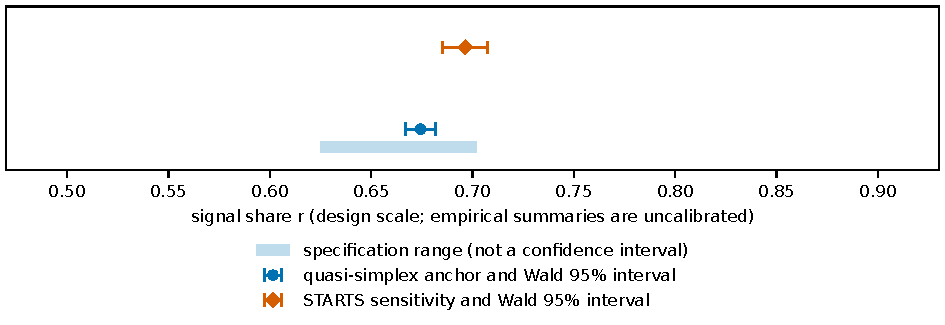
\includegraphics[width=\textwidth]{generated/J6_shp_anchor.pdf}
\caption{Reliability summaries for the Swiss Household Panel trust item. The quasi-simplex anchor and the STARTS point estimate refer to the \resultnum{v4.protocol.shp.anchor_year}{2004} wave and have Wald 95\% intervals. The shaded specification range spans the nine Heise triplet estimates over 1999--2009, from \resultnum{v4.shp.env_lo}{0.625} (2003--2005) to \resultnum{v4.shp.env_hi}{0.702} (2007--2009); it is not a confidence interval. The anchor is placed on the signal-share axis without calibrating it to the design.}\label{fig:shp-anchor}
\end{figure}


\clearpage


\section{Implementation verification}\label{sec:verification}
% Implementation verification (Section S9). Moved from sections/verification.tex
% and sections/supplement.tex of the rule-assembled attempt; the main-text
% summary, whose every claim reappears in the record below, was merged into the
% overview during the journal revision (agent S, 2026-10-13). Test names and
% repository paths were replaced by a pointer to the archive README; claim
% markers (VERxx, AVxx, RCxx) refer to rows in claim-evidence.md.
\phantomsection\label{sec:verification-summary}\phantomsection\label{supp:verification-details}

Verification checks whether the implementation does what the frozen protocol specifies; it does not validate the social mechanism against data. Three layers checked the implementation before any confirmatory seed was used: unit tests, the procedural gates and a freeze preflight. Two docking studies then compared independent implementations with the project code. Three claims of different strength follow from this record, and they should not be confused. % VER01
\begin{itemize}
\item \emph{Intended determinism.} Execution is bound to the recorded environment: the freeze record binds the interpreter, NumPy, the lock file, the platform, single-threaded linear algebra and a numerical probe, and the runners refuse to start in any other environment. Within that environment and the frozen tree, the tests and outputs are designed to agree byte for byte; this is a property of the design, documented by no separate test-run record. % VER14 AV05
\item \emph{Demonstrated component agreement.} The docking studies showed agreement between independent implementations and the project code for specified components and cases, at reduced sizes, and a second host reproduced three G0 tasks to within $7.9\times10^{-12}$ in continuous values. These are checks of parts, not a reproduction of the release.
\item \emph{Unverified full-release replay.} Full-release bitwise replay has not been independently demonstrated, and the recorded checks on Linux failed their declared criteria. Since an operating-system update of 9 October 2026, after the run, the bound machine itself no longer passes the freeze check (Section~\ref{sec:verification-limits}). The release wrapper and the reporting loader also lie outside the frozen code closure (Section~\ref{sec:record-history}). % VER15
\end{itemize}
The README of the archived code lists every test by the property it checks and gives the commands of the runners, the preflight and the reporting steps. Table~\ref{tab:audit-map} (Section~\ref{sec:rule-record}) maps each kind of claim to its public evidence, to what was not kept and to what was checked independently.

\subsection{Test suite}

% VER02
The unit tests belong to the frozen code closure and are grouped here by the property they check; the archive README names them.
\begin{itemize}
\item \emph{Identities (the identity unit tests, G1a).} At full $N$, the zero-strength influence arm and persistence models A, B, D and E must coincide byte for byte. This covers the mask, measured, observed and selected features, in the matching and validation phases, on both attempts, and across the main, mobility, persistent-style, conditioning and 24-step variants. The optimized transport must reproduce the earlier generator's bytes, and the selected features must be byte-identical between implementations. An anchor-exact fit must give zero shifts and zero nuisance variance.
\item \emph{Persistence laws.} Tests check the declared transported laws of B and E, and the degeneracy at $\omega=1$, which is independent of strength and carries no identity claim.
\item \emph{Profile solver.} Tests cover roots on every face and corner; impossible targets, non-finite values and exact budget counting; non-monotone and flat profiles; degenerate secants; two historical stall regressions; the quarter-standard-error acceptance rule; the budget of 96 actual evaluations; and the rule that an endpoint reached without a solver step is labeled \code{boundary}.
\item \emph{Validation and retry.} Tests check the combined-variance validation rule and check that a validation failure leads to a single retry, which keeps both attempts. That the retry happens only after a validation failure and has its own budget is tested only through two pre-freeze scripts, one that checks recorded matching measurements and one that projects the compute cost. Neither property is tested on the fitting code, in which each attempt receives its own budget of 96 evaluations by construction.
\item \emph{Nuisance propagation.} The mean-feature shift predicted at a fixed test point must match regenerated panels within 5\% at the vector level. Further tests cover projection with lag-1 priority, a centered variance with cluster resampling, and uncentered boundary draws.
\item \emph{Band, censoring and scheduling.} Tests cover the nine-strength band, the zero-strength check when the cell at $a=0$ is available (no test checks the rule with that cell unavailable), censoring only across gaps, the survival of other units' boundaries when one unit is invalid, the fixed tier order with its barriers, and the frozen runner's refusal to release before the original deadline. These tests describe the frozen runner, while the linked release amendment is implemented by a later wrapper.
\item \emph{Gate criteria and seeds.} Tests check that failures stay in the denominators, that the finite-difference check uses one median per cell, that the pooled allowance scales with the allocated cells, that the nuisance-variance check reuses the baseline seeds, and that seed domains do not alias, with the confirmatory namespaces reserved. A separate seed-role audit record enumerates seed materials across gate plans and namespaces to check for collisions.
\end{itemize}
% VER14
The test suite depends on the environment, so byte-level checks are expected to hold only in the bound environment; the Linux failures of the frozen-calibration byte test are described under the environment diagnostics below.

\subsection{Environment diagnostics and reproduction limits}\label{sec:verification-limits}

Bitwise agreement is intended only within the bound environment and the frozen tree; no separate test-run record documents it, and complete-run replay has not been independently demonstrated. Later revisions of the repository change the dependency declaration and the lock file, which are in the bound code closure, and add Python files that the preflight also hashes, so the preflight fails on them. % AV05
On Linux x86-64 (Python 3.12.3, NumPy 2.5.3 from the lock), 538 study tests pass and 3 fail, and the same three failures reproduce in a clean worktree of revision \texttt{37513841}: the two cases of the frozen-calibration byte-hash test ($N=600$ and $N=10{,}626$) and one profile-solver test. % AV06
The cause has not been verified; the working hypothesis is that the recorded hashes were generated on macOS and that floating-point arithmetic differs between platforms. % AV06
A second host (Linux x86-64, with a different build of Python 3.12.13) replayed three G0 tasks for equivalence only, not as gate evidence. % AV07
All 82 code hashes matched the freeze record, the numerical probe agreed within $6.7\times10^{-16}$, states, decisions and counts were equal, and 1,331,544 continuous values agreed to within $7.9\times10^{-12}$ in absolute terms. % AV07
The pre-declared equivalence criterion nevertheless failed, only on the \code{seed_material_sha256} field of the phase records (4,448 divergences), because that hash is computed over the numerical parameters at which panels are generated; the platform, interpreter and host fields of the run manifests also differ, as expected between hosts. % AV08
Gate stages and tiers were therefore run on the one bound machine. % AV09
On 9 October 2026, after the run, an operating-system update of that machine (macOS 27.0 to 27.0.1) changed its platform string from the value bound in the freeze record, so the frozen preflight would now refuse to run the gate or the tiers there; the reporting steps do not call the preflight (decision log item 270). The bound environment is thus recorded, but the bound machine itself no longer passes the freeze check.

\paragraph{Replication route.}
Every result table and figure of the article except Table~\ref{main-tab:exploratory}, and every table and figure of this resource rendered by the journal export, regenerate from the archived aggregates with the archived scripts. Table~\ref{main-tab:exploratory} is written by hand, with each result number taken from the archived values files. The tables of this resource rendered by the report export are edited copies of report tables that the archived scripts regenerate, and their result numbers keep their value keys. The other tables of Section~\ref{sec:exploratory} were rendered by the exploratory export, which needs the aggregates of the exploratory analyses X3, X4, X6 and X7; these are not archived because they contain host and path records, so those tables cannot be regenerated from the archive. Their values are in the archived values catalog, which is why, unlike the twin, variance and stress-test aggregates, no sanitized copies of them were made. The values of Tables~\ref{tab:supp-x1a} and~\ref{tab:supp-x2} were transcribed without a script from the archived exploratory aggregates (Section~\ref{sec:rule-record}). Re-running the simulation outside the bound environment, including on the bound machine since its update, means calling the library entry points of the frozen code without the runners' freeze check; the archive README describes this route. The outputs are then not bitwise comparable with the released ones. The random seeds are derived from text labels and do not change, but floating-point results can differ in the last digits (in the cross-host replay above, continuous values agreed to within $7.9\times10^{-12}$); record keys that hash the numerical parameters, such as \code{seed_material_sha256}, then differ, and a decision that falls at a tolerance edge can differ too. Agreement of a complete re-run outside the bound environment with the released results, statistically or within the reported bands, has not been demonstrated and must be assessed rather than assumed.

\paragraph{Correction to the exploratory-aggregate README.}
The earlier statement in \code{archive/exploratory/README.md} that every table and figure regenerates except the twin and variance tables is too broad for this journal version. The applicable scope is given above: article Table~\ref{main-tab:exploratory} is written by hand, and the supplementary tables rendered by the exploratory export cannot be regenerated from the archive because the necessary aggregates are not archived. Their reported values remain available as described above. This correction supersedes that statement without modifying the preserved sanitized aggregates or their original README.

\subsection{Gates and preflight}

% VER03
The validation gate (Section~\ref{sec:odd}, Submodel~14) checks the procedure end to end; its stages, criteria and outcomes are in Section~\ref{sec:record-gate}. The release wrapper and the reporting loader lie outside the frozen code closure, and the repaired summary of the zero-strength band check is stored outside the seal (Section~\ref{sec:record-history}); the actual release time is held in a separate release record (Section~\ref{sec:record-execution}).

% VER04
Before any gate stage or tier runs, the preflight compares the working tree with the freeze record. It requires:
\begin{itemize}
\item schema 2 and status \code{frozen};
\item SHA-256 equality for every file in the bound code closure, including the lock file, and for the criteria and inventory artifacts;
\item agreement of the criteria record with the criteria code and calibration script;
\item hashes of the amendment, specification, revision, review findings and both decision records;
\item eight workers, eight shards and single-threaded BLAS;
\item the recorded interpreter, NumPy, platform and lock environment;
\item agreement of a numerical probe within absolute tolerance $10^{-12}$.
\end{itemize}
A second binding record, created after G0 and before G2, must also exist. It binds the freeze record, the G0 statuses, the criteria record, the G2 cell allocation and the measured G0 gap rate, and is checked against them before G2. Tests check that the runners refuse to start without these records or with stale or changed inputs.

\subsection{Independent docking}\label{sec:verification-docking}

% VER06
Two clean-room docking studies compared independent implementations with the project code at the frozen revision \texttt{37513841}. Each independent implementation was written from the protocol and specification documents alone, without opening the project's source, tests or experiment scripts. Its first-phase readings of ambiguous points were committed before any project source was read, and readings added after the comparison are marked as such. A comparison plan was committed before any comparison ran. In the model study, a timing probe had earlier printed mean lag correlations of 50 project panels in two cells, which Section~\ref{sec:record-exposure} lists as exposure; no margin or cell was chosen from it. Neither study ran a gate stage or tier or used a reserved confirmatory seed namespace. The phase commits in the repository were reconstructed from the session transcripts in their original order; the original commit objects were not pushed, which limits the strength of a clean-room claim. The docking reports and reconstruction notes are in the archive.

% VER07
The first study docked the generative model. With shared seeds, latent trajectories were bitwise identical for the influence arm at $a\in\{0,0.03,0.30\}$ and for persistence models A, B, D and E, in 20 of 20 seeds per case. In a post hoc check not in the pre-declared plan, the ordinal discretizers were also byte-identical given the same continuous responses and mask. At the level of laws ($N=1{,}002$, 11 waves, 25 cells, 1,000 panels per implementation and cell), all 150 primary endpoints were equivalent by two one-sided tests with a margin of 0.20 standard deviations per panel. None of 2,334 secondary difference tests rejected after Holm correction. For the discriminator, run at reduced training and test sizes in three cells with 50 replicates each, mean AUCs differed by at most 0.002 (equivalence margin 0.02). On identical features, the two LDA implementations differed by at most $9\times10^{-5}$. These reduced-size AUCs are not estimates of $\mathcal A(a,r)$.

% VER08
Two specification ambiguities affected numerical output, both negligibly. The first concerned the LDA standardization divisor (the project uses the population standard deviation). The second concerned the normalization of the heteroscedastic error in C (the project uses the empirical mean over the panel, which differed from the analytic expectation by a relative $1.6\times10^{-4}$). No discrepancy in the docked scope was classified as a code--specification divergence. The study did not dock matching, nuisance propagation, bootstrap bands, gates, seeds or sealing; the latent, error-free ordinal, latent-rank and mobility channels; the persistent-style, conditioning, anchoring, attraction-only and 24-step sensitivities; the lag-one feasibility rule; or production sizes. Its law-level resolution (0.20 standard deviations, about 0.002--0.005 in units of the ordinal lag correlations) is far coarser than the matching tolerance. Heaping and masks agree only in law because the two implementations consume random draws in a different order.

% VER09
The second study docked the inference and calibration machinery: the profile solver, acceptance tolerance, independent validation and retry, local nuisance propagation, cluster bootstrap, band, gap and gate rules, and the Jeffreys stop rule. Both implementations received identical synthetic inputs, including adversarial ones. Tolerances, validation decisions, the retry protocol, projected parameter shifts (2,500 cases), finite differences, nuisance draws, $V_{\mathrm{nuis}}$, bootstrap standard errors, failure allowances and the shared-seed stop-rule probability agreed to $10^{-12}$ or better, most bitwise. Exceptions were reporting-only differences at 0/0 and non-finite inputs and in one Monte Carlo standard-error formula. At a non-positive Schur slope, the project stops with an error where the docking solves the projection; this was classified as a specification ambiguity. For the nuisance draws, the docking implementation was given the project's discriminator.

% VER10
Solver status agreed in 16 of 22 synthetic cases; the report's count of 17 is corrected in the study's reconstruction note. All six divergences (cases 5, 6, 9, 10, 17 and 21 of the docking record) were traced to four specification ambiguities, which that record lists. In three cases the project reports \code{no-L1-root} where the docking reports a family limit; both labels are gaps. The project can also report family limits within the profile solver, so these cases do not imply that such limits arise only in the feasibility screen. In one case with discrete steps the two labels are \code{numerical-limit} and \code{ill-conditioned}. In one case a root lies within tolerance of the endpoint and is labeled \code{interior} by the project and \code{boundary} by the docking; both are accepted states. In the hump-shaped profile case, the project accepted a genuine interior root after sampling only $\eta\leq0.01$, whereas the docking evaluated $\eta=0.8$ early, detected the non-monotone profile and returned a gap. This is the only divergence that changes the accept-or-gap decision.

% VER11
The band critical values differed, by up to a factor of 2.1, in the ten random cases compared. A post hoc analysis reproduced the project's values exactly in all ten cases from three readings: the logit standard error evaluated at each replicate rather than at $\hat p$, replicates centered on the point estimate, and the \texttt{higher} quantile rule. The per-replicate standard error dominates; in one case the plug-in reading gave a critical value of 7.15 and the project's reading 3.37. The project's band code reproduces the frozen v1 band exactly, and Section~\ref{sec:design-details} describes that reading. Inversion, gap, censoring and zero-strength rules agreed in 9 of 11 cases. In the other two, adjacent to a gap, the project censors the sustained boundary where the docking declares the first strength above the gap, which is the more conservative reading. No divergence was classified as a probable project error.

% VER12
The second study left matching on real panels, the feasibility screen and the mean-feature Jacobian on real realizations unverified. It also left unverified the control path that inherits $\eta$ in the nuisance draws; the amplification and covariance diagnostics; and the calibrated G2 dispersion thresholds and the G2c ratio beyond failure counts. G1b, G1c, the G0 status projection that feeds the stop rule, the curve runner, scheduler, sealing, seed derivation and collision audit also remained unverified. The study did not verify solver efficiency on real targets, since evaluation counts were reported but not compared, or the statistical coverage of either band reading. The project's reading is the one that the band calibration (G1b) tests.

% VER13
Docking establishes agreement between two implementations of the same written specification in the scope docked. Where both made the same choice at an ambiguous point, it cannot detect an error in the specification itself or a misreading shared by both authors. The two implementations are also less independent than those of two human teams: the frozen code was implemented with AI coding agents (Codex and Claude) and the docking implementations were written by Claude (Section~\ref{sec:ai}), so a misreading shared by those models would go undetected. Docking is not validation of the social mechanism, not an estimate of coverage and not a substitute for the gates.


\section{Positioning search record}\label{sec:search}
% Positioning search record (Section S10). Moved from sections/supplement.tex
% (SUP12, SUP13) and sections/related-work.tex (R56, R57, R58, R63) of the
% rule-assembled attempt; cleaned during the journal revision (agent S,
% 2026-10-13): repository paths replaced by a pointer to the archive.
\phantomsection\label{supp:search-record}

The positioning of the article (Section~\ref{main-sec:background}) rests partly on a documented but limited search for studies that combine the components of this design. This section records how the search was run and what it can and cannot support.

\paragraph{Declaration and runs.}
% SUP12 R56
Ten English-language queries were declared on 27 September 2026, before any run. The declaration commit in the project repository, \texttt{987acded}, is a local reconstruction of the commit made in the cloud session that ran the search. Each query was run unchanged on OpenAlex and Semantic Scholar; for arXiv, the declaration fixed a Boolean translation of each query. The first 20 results per query and service were screened. OpenAlex returned a rate-limit error on 27 September at 22:59 UTC, and its ten queries ran on 28 September between 00:01 and 00:16 UTC. Two Semantic Scholar queries failed on rate limits. The arXiv export API returned HTTP 406 for all ten Boolean translations, which were then run through the arXiv site search (all metadata fields, terms joined by AND), the closest available substitute rather than the declared API route. The record lists 40 runs and 399 screened titles: 391 were not relevant, five relevant records corresponded to four works already in the antecedent matrix, and three were new \cite{carpentras2022,xu2021sensitivity,advani2018credibly}.

\paragraph{Reconstruction of the record.}
% SUP13 R63
The original per-run record did not leave the cloud session. It was reconstructed on 28 September 2026 from the result lists printed in the session transcript, by rerunning the session's own screening scripts on those printouts without changing any decision, and it reproduces the totals above. It has gaps: no run carries a URL or retrieval time, and run times are known only for OpenAlex; DOIs are missing for all 200 OpenAlex hits and for 24 of the 160 Semantic Scholar hits (16 printed with an arXiv identifier, 8 with neither); Semantic Scholar identifiers are truncated for some queries and replaced by placeholders for others; and titles were printed truncated at 100 to 115 characters. The reconstructed record, its dossier and a description of each gap are archived with the journal sources.

\paragraph{Coverage and what the search supports.}
% R57 R58
Coverage was limited. Two Semantic Scholar queries failed on rate limits, and the unavailable arXiv API was replaced by the site search. OpenAlex relevance ranking, which weights citations, favored highly cited work from other fields. Several of the closest works surfaced only through citation, and theses, non-English literature and survey methodology were not searched. Within this search and the works read, no study was identified that estimates the minimum influence strength at which individual panel trajectories become distinguishable from a set of matched persistence models without a network, as a function of the signal share of the response channel. Absence from a limited search is not proof of absence, and the article makes no priority claim.


\section{Use of generative AI}\label{sec:ai}
% Use of generative AI in detail (Section S11). Written during the journal
% revision (agent S, 2026-10-13) from sections/ai-use.tex (M54, M55), the
% governance statements of sections/methods.tex and sections/supplement.tex
% (M83, M89) and the AI statements of the ODD of the rule-assembled attempt.
% Governance claims are not stronger than those records state.
% Round 5 (2026-10-14): second simulated panel recorded (Codex model from its
% run log); "other venues" dropped; closing sentence aligned with the delegation.
% Round 6: pre-submission checks and the third simulated panel (round6.md item 8).

AI agents were used throughout this project. The project's AI-disclosure evidence table, cited by its claim--evidence map, links each role that AI agents played before the results became available to the records that document it and states where a record does not identify the exact model; neither the table nor the map is part of the archive. The agents are not authors. % M54

\paragraph{Roles before the results became available.}
Claude models (Anthropic), recorded mainly as \code{claude-opus-5-5}, reviewed the candidate designs, exchanged amendment proposals and critiques with Codex before the v4 successor was adopted, challenged the focused literature review, ran the positioning search (Section~\ref{sec:search}) and audited the claim--evidence map. % M54
In separate sessions and from the specification documents only, Claude also wrote the two independent implementations used for docking (Section~\ref{sec:verification}). A Claude Code session coordinated the project, drafted amendment v4.4, wrote decision records and corrections, and integrated the drafts into the manuscript. % M55
GPT-6 models through Codex (OpenAI), recorded as \code{gpt-6-astra} and \code{gpt-6.1-sol} where identified, acquired, screened and synthesized the literature of the focused review, wrote internal adversarial reviews, and implemented the reporting, export, manuscript-assembly and packaging code. % M54
The frozen simulation and inference code (Git revision \texttt{37513841}) was implemented with AI coding agents, Codex and Claude, under the first author's direction. The records do not link that original implementation to specific sessions or model versions (item Q4-07 of the project's AI-disclosure evidence table). The code was checked by its unit tests, by the validation gate and by the two separate re-implementations written from the specifications for docking (Section~\ref{sec:verification}).
Claude and Codex sessions drafted and revised the text of every section of the rule-assembled manuscript, including the model description and the conditional text of the abstract, Results, Discussion and Conclusion, which was written before the results became available. A deterministic program assembled the first manuscript from that text and the results; after the results became available, the wording of the assembled text was corrected in two recorded batches without changing any value or reading (Section~\ref{sec:rule-record}). % M54
Where a record does not identify the exact model, the evidence table says so. The internal AI reviews are model outputs, not peer review. % M54

\paragraph{Delegated decisions and ratification.}
From 24 September 2026 the first author delegated decisions to the coordinating agent, a Claude Code session, which recorded each delegated decision and its justification for later ratification (decision log items 10, 20 and 21). Some protocol decisions were proposed by AI agents and adopted under that delegation. The v1 protocol was frozen by the coordinating agent, and its freeze record marks it as pending ratification (decision log item 18). The v4 successor was adopted after two amendment proposals and two critiques by Codex and Claude, and its decision specification records a delegated agent decision pending the first author's ratification (decision log item 19). The seven choices left open by the review of the declaration of the exploratory analyses X3--X7 were confirmed by the coordinating agent before any implementation. These decisions took effect under the delegation and before their ratification, as their records state. Both authors ratified them, together with the later amendments, on 1 October 2026, before the results became available (decision log item 161); Section~\ref{sec:record-governance} gives the scope of that ratification. Amendment v4.4 was proposed by the coordinating Claude Code session and took effect only after the first author approved it (Section~\ref{sec:record-execution}). The authors approved the study design and its amendments and take full responsibility for the content of the article. % M54 M83
The empirical reliability anchor was computed on the first author's computer, launched under delegation without the restricted SHP microdata entering the context of any AI agent; only the approved aggregate left the restricted environment (Section~\ref{sec:shp}). The concise disclosure in the article summarizes these roles; it does not replace the distinctions between implementation tests, component agreement and full independent reproduction in Section~\ref{sec:verification}.

\paragraph{Roles after the results became available.}
On 9 October 2026, four AI reviews of the rule-assembled PDF were obtained, in the roles of an editor, a domain referee and a methods referee (Claude, recorded as Opus 5.5) and of an adversarial referee (Codex, recorded as \code{gpt-6.1-sol}). They are model outputs, not peer review. The methods review prompted the reading, marked in Section~\ref{main-sec:methods-identification} of the article as made after the results became available, that the serially correlated input from fixed contacts may be the main source of separation. On 13 October 2026 the first author delegated the revision of the text into the journal version to AI agents coordinated by a Claude Code session (\code{claude-opus-5-5}), under the rules described in Section~\ref{sec:rule-record}: the numbers stay bound to the released values, new tabulations are generated by code from released artifacts, readings made after the results became available are marked, and the protocol, criteria, seeds and results are unchanged. On the same day a second round of four AI reviews, in the same roles and with the same recorded models, read the journal version and this resource, the adversarial review with an independent numeric audit of the bound and transcribed values; the revisions they prompted change wording, add tabulations of released values and add the analytic values of the kernel marked in Section~\ref{sec:dd-drift-mean}. Later that day a simulated review panel of AI reviewers (Claude agents of the coordinating session and, for the statistical referee, Codex recorded as \code{gpt-6.1-sol}) assessed the journal version; the revisions it prompted again change wording, add tabulations of released values and add the audit map of Section~\ref{sec:rule-record}. A second simulated panel, with the same roles and models, then read the revised version; the revisions it prompted change wording, add tabulations of released values, among them the fitted parameters of the free-share analysis and the lag pattern of the stress test, and add references. On 14 October 2026, before submission, AI reviewers checked the value bindings, the export code of the journal tables and the text, and a third simulated panel, in the same roles, read the revised version; the revisions they prompted change wording and layout and correct the statement of which tables regenerate from the archive (Section~\ref{sec:verification}). On 20 October 2026, under the first author's authorization, Codex agents (recorded as \code{gpt-6.1-sol}) applied the second author's editorial comments to the article and this resource, and two further Codex reviews with the same recorded model checked the revised interpretation; the revisions change the title, the abstract and the wording and structure of the article, move the persistence-model equations and classifier details into this resource (Sections~\ref{sec:dd-channels} and~\ref{sec:dd-classifier}) and correct the statement on the error-free control at $r=0.50$, without changing any value, protocol or result. On 29 October 2026 a Claude Code session (\code{claude-opus-5-5}) filled the funding, ethics and approval declarations from the first author's confirmations; one Codex and one Claude reviewer then checked them, and their comments led to small wording corrections on 30 October 2026. The journal text, including this resource, was thus revised after the results became available by AI agents, under the first author's delegation and the authors' review.


\section{Prespecified reading rules and the rule-assembled record}\label{sec:rule-record}
% Prespecified reading rules and the rule-assembled record (Section S12).
% Written during the journal revision (agent S, 2026-10-13) from the assembly
% record of attempt assembly-xdj406x0, the assembly guide of the manuscript
% pipeline, the repin receipts of rounds T58 and T59 and the decision log
% (items 246-269). The counts of selected and excluded blocks come from the
% attempt's assembly record (keys j.rule.*). Round 5 (2026-10-14): the audit map
% names the per-cell stress-test lags (tab:x5-lags) and the free-share search
% points, among them the trial point at r + 0.01 (j.x3.plus.*).

\paragraph{Prespecified reading rules.}
The reading rules and the conditional text that reports and interprets the results were written before the results became available; the wording corrections made afterwards are described below. The Results, the Discussion, the Conclusion and the abstract were drafted as conditional blocks: each block carries a selection condition on the released facts (for example, whether the validation gate passed, whether a unit is complete and valid, or whether the condition for comparing persistence models is met) and slots for the released values. The interpretation rules that these blocks apply were fixed before the results as well, including the readings of the exploratory analyses under the restrictions of 29 September 2026 (Section~\ref{sec:exploratory}). The blocks, the rule registry and the source drafts were pinned by SHA-256, so that any later change to a block changes a recorded digest and needs a receipt. This design guards against choosing, after seeing the results, which reading to report.

\paragraph{The rule-assembled record.}
When the results became available, a deterministic program assembled a first manuscript: it evaluated every rule on the released values and facts, selected the applicable blocks, filled their slots with the bound values and refused to proceed on any missing value or inconsistency. For the attempt kept as the record (identifier \texttt{assembly-xdj406x0}), it selected \resultnum{j.rule.blocks_selected}{111} blocks, excluded \resultnum{j.rule.blocks_excluded}{142} and refused none, and it wrote an assembly record with the digests of the values, the facts, the rules, the source drafts and every output file.
Before that attempt, once the assembled text with the released values had been read, its wording was corrected in two recorded batches (8 and 9 October 2026; decision log items 246--252 and 258--262). The corrections changed no value or reading and kept the identity, selection condition, slots and order of every rule; their receipts list every changed span and verify the rule fields and the scientific predicates; and their record states that no reading goes beyond the frozen rules. They changed wording and layout: for example, a Conclusion sentence for the case in which every share falls in one region, the statement of the G1a status, and the placement of the supplement after the references. The blocks as written before the results remain in the repository history.
The compiled rule-assembled manuscript has 95 pages, combining the article, the model description and the supplement; its PDF was produced on 9 October 2026 and has SHA-256 \texttt{c1a255dbc2aca3b1}\allowbreak\texttt{0129b4c58b1494cf}\allowbreak\texttt{5f70cf74ada23916}\allowbreak\texttt{74367d9a9b1e1aee}. This PDF, the pre-written blocks, the rule registry and the assembly record are archived with the code as the prespecified record, unchanged; the assembled TeX files are not archived, but the assembly record holds their digests. The receipts of the two correction batches are archived with the journal sources, and the article's Data and code availability statement gives the archive's DOI.

\paragraph{The journal text.}
The article and this resource were edited after the results became available. Four AI reviews of the rule-assembled PDF, obtained on 9 October 2026, found the science reviewable but the text written as a protocol audit rather than for the journal's readers (Section~\ref{sec:ai}). From 13 October 2026 the text was rewritten for those readers: the article was shortened and restructured, internal codes were replaced by plain names (Section~\ref{sec:glossary}), and the audit material, the full model description and the exploratory analyses moved to this resource. The edits follow fixed rules. Numbers taken from the results are printed through value keys: keys of the values file of the rule-assembled attempt, used unchanged; keys of new tabulations of released quantities, computed by code from the released artifacts; and keys of a small file of values transcribed from archived exploratory, protocol and assembly records, each with its source (two of its keys restate, for the prose, the magnitudes of generated keys). A check run at every build compares each printed key with its value. The values of Tables~\ref{tab:supp-x1a} and~\ref{tab:supp-x2}, and some counts and values in the prose, chiefly in Sections~\ref{sec:record}, \ref{sec:exploratory}, \ref{sec:verification} and~\ref{sec:search}, have no key: they are transcribed from exploratory, protocol, verification and search records. These are archived except three that contain home paths, private host names or host records: the coverage-check report of protocol v1 (Section~\ref{sec:record-history}), the record of the byte-for-byte check that preceded the twin's boundary analysis (Section~\ref{sec:x1-x2}) and the record of the second-host replay (Section~\ref{sec:verification-limits}); a few statements rest instead on the authors' private decision log, whose item numbers they cite. The values of Tables~\ref{tab:supp-x1a} and~\ref{tab:supp-x2} and the unkeyed counts and values of the exploratory and verification passages were compared with their source records in a separate audit of the journal version (Section~\ref{sec:ai}). The protocol, criteria, seeds and results are not changed. Readings that the rule-assembled record does not contain, made after the results became available, are marked as such in the article and in this resource. A reader can compare the two texts in the archive; where they differ in interpretation, the rule-assembled record is the prespecified one.

\paragraph{Exploratory aggregates.}
The aggregate results of the exploratory analyses X1a, X1b, X2 and X5 are archived as sanitized copies, with host and path fields removed, in the folder \code{archive/exploratory} next to the journal sources; its README lists every removed field and the SHA-256 of each original and sanitized file. The results of X3, X4, X6 and X7 are in the archived values catalog.

\paragraph{Audit map.}
Table~\ref{tab:audit-map} maps each kind of claim to the public evidence behind it, to what was not kept or not made public, and to what was checked independently of the project code. It adds no evidence; it says where to look and what cannot be checked from the archive.

\begingroup\footnotesize
\setlength{\LTcapwidth}{\textwidth}
\begin{longtable}{@{}>{\raggedright\arraybackslash}p{0.155\textwidth}>{\raggedright\arraybackslash}p{0.26\textwidth}>{\raggedright\arraybackslash}p{0.25\textwidth}>{\raggedright\arraybackslash}p{0.225\textwidth}@{}}
\caption{Audit map: public evidence, what was not kept and what was checked independently, by kind of claim. Section numbers refer to this resource}\label{tab:audit-map}\\
\toprule
Claim & Public evidence & Not kept or not public & Checked independently \\
\midrule
\endfirsthead
\caption[]{Audit map (continued)}\\
\toprule
Claim & Public evidence & Not kept or not public & Checked independently \\
\midrule
\endhead
\botrule
\endfoot
Boundaries, bands and unit statuses (all 414 units) & Released curves, which also hold each cell's fitted parameters, nuisance variance and fit attempts; their public projection (per cell, point AUC and band limits; per unit, critical value, status, gap kinds and boundaries); values catalog, Online Resource~2; Sections~\ref{sec:inventory} and~\ref{sec:additional} & Per cell: score standard errors and mean lag correlations; the per-panel features stay in the sealed store & Band, inversion, gap and censoring rules, on synthetic inputs (Section~\ref{sec:verification-docking}); the released curves were not recomputed independently \\[3pt]
Validation gate & Criterion values, counts, ratios and verdicts of the five recorded stages; criteria record and calibration script (Section~\ref{sec:record-gate}) & Per-repetition estimates of the dispersion and nuisance-variance checks (sealed, not analyzed); no run record of the identity unit tests & Gate rules, allowances and stop rule, on synthetic inputs; three zero-strength fitting-check tasks replayed on a second host, for equivalence only; the band calibration on synthetic scores, the zero-strength band check and the status projection of the fitting check not docked \\[3pt]
Prespecification and exposure & Freeze records, protocol, criteria, seeds and inventory bound by SHA-256 (Table~\ref{tab:record-identifiers}); the rule-assembled record (this section) & External timestamps (dates rest on the repository history); the authors' decision log, a private record & Any reader can recompute the hashes of the files archived unredacted; four bound files are archived only as redacted copies, and some files bound by the v1 and SHP freeze records are not archived (Section~\ref{sec:record}); no third-party registration exists \\[3pt]
Exploratory analyses & Sanitized aggregates of the twin, variance and stress-test analyses next to the journal sources, with B's fitted parameters and both arms' mean lag correlations per stress-test cell (Table~\ref{tab:x5-lags}); the other analyses in the values catalog, with the free-share fits, the share-search points (among them the trial point \resultnum{j.x3.plus.offset}{0.01} above the design share) and mean lag correlations per cell (Section~\ref{sec:exploratory}) & Matching uncertainty of the free-share fits (not computed); truth-precision sensitivity of the coverage check (not triggered); a script for Tables~\ref{tab:supp-x1a} and~\ref{tab:supp-x2}, which are transcribed & Transcribed values compared with their records in a separate audit of the journal version (this section) \\[3pt]
Empirical reliability anchor & Approved aggregate output: estimates, standard errors, fit statistics, counts and crosswalk ranges (Section~\ref{sec:shp}) & SHP microdata (data-use contract; available from FORS); not printed here: polychoric estimates, heaping shares and the positive-strength crosswalk cells & Not re-estimated independently \\[3pt]
Implementation & Code at the frozen revision with its tests; docking reports and reconstruction notes (Section~\ref{sec:verification}) & Bitwise replay of the full release not demonstrated; three test failures on Linux; the bound machine fails the freeze check since 9 October 2026 & Docking of the generative model and of the inference machinery within the scope of Section~\ref{sec:verification-docking}, by implementations written with AI models of the same families as the project code \\
\end{longtable}
\endgroup

\clearpage


\phantomsection\addcontentsline{toc}{section}{References}
\bibliography{references}

\end{document}
